\documentclass[12pt, a4paper, german]{book}
% \usepackage[utf8x]{inputenc}
% \usepackage{ucs} % unicode
%\usepackage[T1]{fontenc}
\usepackage{t1enc}
% \usepackage{type1cm}
\usepackage[german]{babel}
\usepackage{url}
 
\usepackage{eurosym} 
\usepackage{amsmath, amssymb}
\usepackage{graphicx}
\usepackage{natbib}
\usepackage{rotating}
\usepackage{marginnote}

\usepackage{ifpdf}
\ifpdf
\usepackage{xmpincl}
\usepackage[pdftex]{hyperref}
\hypersetup{
    colorlinks,
    citecolor=black,
    filecolor=black,
    linkcolor=black,
    urlcolor=black,
    bookmarksopen=true,     % Gliederung öffnen im AR
    bookmarksnumbered=true, % Kapitel-Nummerierung im Inhaltsverzeichniss anzeigen
    bookmarksopenlevel=1,   % Tiefe der geöffneten Gliederung für den AR
    pdfstartview=FitV,       % Fit, FitH=breite, FitV=hoehe, FitBH
    pdfpagemode=UseOutlines, % FullScreen, UseNone, UseOutlines, UseThumbs 
}
\usepackage{bookmark}
\includexmp{Vorlesung_Entscheidungstheorie}
\pdfinfo{
  /Author (Eckhart Arnold)
  /Title (Vorlesungsskript: Grundlagen des Entscheidens I)
  /Subject (Eine Einführung in die mathematische Entscheidungstheorie)
  /Keywords (Entscheidungstheorie, Spieltheorie, Sozialwahltheorie, Philosophie der Wahrscheinlichkeiten)
}
\else
\usepackage{hyperref}
\fi


% \usepackage{array}
% \newcolumntype{v}[1]{>{\raggedright\hspace{0pt}}p{#1}}

\numberwithin{equation}{section}

%\newcommand\marginline[1]{\marginpar[\raggedleft{\scriptsize
%#1}]{\raggedright{\scriptsize #1}}}
 
\renewcommand{\marginfont}{\scriptsize}
\newcommand{\marginline}{\marginnote}
 
\hyphenation{Er-wart-ungs-nut-zen-ei-gen-schaft 
             Er-wart-ungs-nut-zen-hy-po-the-se   
             Er-wart-ungs-nut-zen
             Nut-zen-funk-tion   
             Nut-zen-funk-tion-en 
             Ent-scheid-ungs-re-gel
             vor-aus-setz-ungs-arm
             Geld-wert  Geld-werte
             sinn-voll-ere
             Aller-dings}

\sloppy

\begin{document}

%\title{Vorlesung: Grundlagen des Entscheidens I}

%\author{Eckhart Arnold}
%\date{Stand: 6. Juli 2009}

%\maketitle

\begin{titlepage}
\begin{center}

\ { } 

\vspace{0.5cm}

{\Large Vorlesung: Grundlagen des Entscheidens I}

\vspace{0.75cm}

Sommersemester 2009

\vspace{0.5cm}

Stand: 6. Juli 2009 \\~\\
Hinweis: Das Skript wurde bisher noch wenig Korrektur gelesen und das letzte Kapitel
fehlt leider ganz. Es enthält jedem Menge Tippfehler und auch vereinzelte sachliche Fehler
können nicht ganz ausgeschlossen werden. Trotzdem: Viel Spaß beim Durcharbeiten!

\vspace{0.5cm}

Dozent: Dr. Eckhart Arnold

\vspace{1cm}


\includegraphics[width=6cm]{Grafiken/pe_logo.eps}

\vspace{0.25cm}

{\Large Universität Bayreuth}

\vspace{1.75cm}

\includegraphics[width=2.5cm]{Grafiken/CC-BY-SA.eps}

\vspace{0.5cm}

\begin{small}

Dieses Material ist frei zugänglich und darf unter den Bedingungen der
Creative-Commons-Lizenz BY-SA 4.0 weiter gegeben werden.

\vspace{0.5cm}

Die Klausel BY-SA besagt: Der Name des Autors muss bei abgeleiteten Werken
genannt werden, und abgeleitete Werke oder Kopien müssen ebenfalls unter
dieser Lizenz weitergegeben werden.

\end{small}

\end{center}

\end{titlepage}

\tableofcontents
\newpage 
 
\setlength{\marginparwidth}{2cm}

\chapter*{Vorwort}

Dieses Skript gehört zur Vorlesung "`Grundlagen des Entscheidens I"', die ich im
Sommersemester 2008 in Bayreuth gehalten habe. Inhaltlich habe ich mich dabei
weitgehend an die bewährte Einführung von {\em Micheal D. Resnik: Choices. An
Introduction to Decision Theory, University of Minnesota Press, 5th ed. 2000
\cite{resnik:1987}} gehalten, die eine ansprechende Stoffauswahl mit nicht
übermäßig schwierigen mathematischen Beweisen verbindet. An vielen Stellen bin
ich aber auch von Resnik abgewichen. So habe ich besonders für die
Wahrscheinlichkeitsrechnung außer gängigen mathematischen Lehrbüchern vor allem
die sehr gelungene Darstellung von Donald Gillies \cite{gillies:2000}
herangezogen. Auch die Darstellung der Spieltheorie stützt sich überweigend auf
andere Quellen. Da ich die Vorlesung zum erstenmal gehalten habe, enthält das
Skript zweifellos noch zahlreiche Flüchtigkeits- und Tippfehler, die ich bei
Gelegenheit noch zu korriegieren hoffe. (Wer Lust hat ein wenig Korrektur zu
lesen, oder wer Fehler, besonders inhaltlicher Art(!) im Skript entdeckt, teile
es mir bitte mit: eckhart\_arnold@hotmail.com) Auch bleibt es nicht aus, dass
ich im Nachhinein viele Dinge anders machen würde. Im einzelnen sehe ich folgende Punkte, an denen sich eine Überarbeitung der Vorlesung bzw. des Konzepts der Vorlesung lohnen würde:

\begin{itemize}
  \item Über der Darstellung des dogmatischen Lehrstoffes ist leider die Kritik
  und die Erörterung von (besseren) Alternativen zu kurz gekommen. Besonders in
  den letzten Abschnitten der Vorlesung, also der Spieltheorie und der
  Sozialwahltheorie, wäre es wichtig noch ausführlicher zu erörtern, warum die
  entsprechenden Ansätze nur eine äußerst begrenzte Sichtweise auf menschliches
  Handeln (Spieltheorie) bzw. politische Ordnung und politische
  Entscheidungsfindung (Sozialwahltheorie) ermöglichen. Hinsichtlich der
  Entscheidungs- und Spieltheorie wäre es sicherlich empfehlenswert auch
  Ansätze aus der Psychologie und der experimentellen Spieltheorie zum
  Verständnis menschlichen Handelns und Entscheidens stärker einzubeziehen. 
  Bei der Sozialwahltheorie, die in dieser
  Vorlesung allerdings nur sehr kurz angerissen wird, würde es lohnend sein, 
  auch alternative Ansätze der Demoktratietheorie anzusprechen, 
  um zu vermeiden, dass ein falsches Bild vom Gegenstandsbereich dieser
  Theorien entsteht. Unweigerlich formen nämlich die Theorien, mit denen wir
  uns beschäftigen, das Gesamtbild des Gegenstandes, auf den sie sich beziehen.
  Ich könnte es mir leicht machen, und die Stoffauswahl durch den Gesichtspunkt
  thematischer Beschränkung auf die formale Entscheidungstheorie verteidigen.
  Aber dagegen rebelliert mein intellektuelles Gewissen. Denn
  wenn die entsprechenden Theorien nur Teilaspekte des Gegenstandes
  abdecken können, dann entsteht beinahe unvermeidlich ein verzerrtes 
  Gesamtbild. Im Extremfall wäre man klüger geblieben, 
  hätte man sich
  gar nicht mit der wissenschaftlichen Theorie abgegeben, sondern sich bloß auf
  den eigenen gesunden Menschenverstand bei der Beurteilung der Sache verlassen. 
  Gerade der Philosophie, die doch immer die übergreifenden Zusammenhänge im
  Auge behalten sollte, steht es nicht an, sich mit thematischer
  Selbstbeschränkung herauszureden.

  \item Was nun die Auswahl der Themen angeht, so scheint mir, dass vor allem
  die Aufnahme der an sich sehr interessanten philosophischen
  Wahrscheinlichkeitstheorien (v. Mises und Ramsey-De Finetti, siehe Kapitel
  \ref{philosophischeWahrscheinlichkeitstheorien}) zu überdenken ist. Nicht so
  sehr wegen der mathematischen und gedanklichen Anspruchshöhe als deshalb,
  weil der Stoff einerseits zwar wohl zum geistigen Hintergrund der
  Entscheidungstheorie gehört aber für die folgenden Themen nicht unbedingt
  vorausgesetzt werden muss und zudem eine eigene, ausführlichere Behandlung
  verdienen würde. 
  
  Ebenfalls zu überdenken scheint mir in diesem Fall die Aufnahme der
  Neumann-Morgensternschen Nutzentheorie (Kapitel \ref{NeumannMorgenstern}).
  Meine Motivation dafür sie aufzunehmen bestand darin, dass sie auch in den
  Lehrbüchern etwa zur Spieltheorie \cite{myerson:1991} auftritt, wobei die
  Motivation zu der doch seltsamen Konstruktion der Lotterien oft etwas im
  Dunkel bleibt. Mir scheint, dass die Neumann-Morgensternsche Nutzentheorie im
  wesentlichen auf einer Illusion beruht, der Illusion nämlich man würde 
  kardinale Nutzenwerte eines Tages so präzise messen können wie die
  Temperatur. Diesen Vergleich zur Physik führen Neumann und
  Morgenstern selbst an, wie irreführende Vergleiche mit der Physik ja immer zu
  den Requisiten mathematikbegeisterter Sozialwissenschaftler gehören. Aber
  nach 60 Jahren -- das Buch von Neumann und Morgenstern erschien 1947 -- sind
  wir von einer präzisen Messung von kardinalen Nutzenwerten immer noch genauso
  weit entfernt wie damals. Wozu soll die gewaltsame mathematische Konstruktion
  kardinaler Nutzenwerte gut sein, wenn man sie doch nicht präziser messen kann als 
  durch die Frage "`Wieviel Geld gibst Du mir dafür?"' Mag sein, dass die
  Neumann-Morgensternsche Nutzentheorie zu den unveräußerlichen Grundlagen der
  Spieltheorie und der Volkswirtschaftslehre gehört. Für sich betrachtet wirkt
  sie eher wie eine müßige mathematische Spielerei.
  
  \item Es hat sich gezeigt, dass besonders die mathematischen Beweise viele
  Leute vor schwer überwindliche Hindernisse stellen. Die didaktisch
  wohlverständliche Aufbereitung mathematischer Beweise stellt dabei eine nicht
  zu unterschätzende Herausforderung dar, die viel Zeit und Mühe erfordert.
  Resnik hat sich in seinem Lehrbuch dankenswerter Weise möglichst einfacher
  Beweisführungen bedient. Ich habe soweit als möglich versucht, die
  Beweisführungen nochmals einfacher und verständlicher darzustellen, aber ich
  möchte nicht behaupten, dass in dieser Hinsicht nicht noch ein Übriges getan
  werden könnte.
  
  Auch wenn es billig klingt, so kann ich in diesem Punkt doch den
  Mathematikunterricht in der Schule nicht ganz von Tadel freihalten, weil man
  dort zwar tüchtig rechnen lernt aber keine richtige Mathematik, d.h. keine
  Beweisführungen.
  
  \item In diesem Zusammenhang ist einzuräumen, dass die Nomenklatur in meinem
  Skript zum Teil uneinheitlich und manchmal ungünstig gewählt ist, besonders
  bei der Wahrscheinlichkeitsrechnung. In der Fachliteratur gibt es
  unterschiedliche Arten die Wahrscheinlichkeitstheorie darzustellen. In
  mathematischen Lehrbüchern ist die Mengenschreibweise üblich, d.h. man
  bezieht die Wahrscheinlichkeiten auf Ereignismengen. In der philosophisch
  orientierten Literatur greift man lieber auf eine aussagenlogische
  Schreibweise zurück. Meist habe ich das letztere gewählt. Für eine zukünftige
  Überarbeitung wäre aber eine einheitliche Schreibweise und dann
  höchstwahrscheinlich die Mengenschreibweise wünschenswert. (In diesem
  Zusammenhang scheint mir, dass die logische "`und"'-Verknüpfung bzw. die
  Schnittmenge mit einigem Gewinn für die Lesbarkeit durch das
  Zeichen "`\&"' statt durch das Zeichen "`$\wedge$"' dargestellt werden kann.)
  Vielleicht wäre darüber hinaus ein kurzer Anhang zur formalen
  Logikschreibweise, deren Kenntnis hier vorausgesetzt wird, empfehlenswert.
\end{itemize}

\begin{flushright}
Eckhart Arnold, Bayreuth, den 25. Juli 2008
\end{flushright}


%\newpage 

\chapter{Techniken des Entscheidens}

\section{Entscheidungstabellen und -bäume}

\subsection{Einleitung}

Die Vorlesung "`Grundlagen des Entscheidens I"' hat das Ziel -- aus
philosophischer Perspektive -- in die Entscheidungs- und Spieltheorie
einzuführen. Dabei geht es vor allem um die Vermittlung von Grundlagen
und elementaren Lösungs- und Rechentechniken, d.h. wir werden
untersuchen, wie man Entscheidungsprobleme als Tabellen oder
Entscheidungsbäume darstellt, wie Entscheidungen unter Risiko (d.h.
bei bekannten Wahrscheinlichkeiten für das Eintreten unbeeinflussbarer
Ereignisse) und unter Unwissen (bei unbekannten Wahrscheinlichkeiten)
getroffen werden können, wie die strategische Interaktion zwischen
mehreren menschlichen Entscheidern mit Hilfe spieltheoretischer
Modelle dargestellt werden kann und vieles mehr. Dabei werden wir uns
immer auch mit den philosophischen Interpretationsfragen dieser
Techniken beschäftigen, sowie mit theoretischen Einwänden, von denen
es zahlreiche gibt.

Ausgespart bleibt in den "`Grundlagen des Entscheidens I"' jedoch
weitgehend die Frage der Anwendung dieser Theorie in verschiedenen
empirischen Wissenschaftsbereichen. Die Anwendbarkeit der Spiel- und
Entscheidungstheorie ist je nach Wissenschaftsbereich mehr oder
weniger stark umstritten. Während sie in der Ökonomie gewissermaßen
kanonisch ist, wird ihr Wert für die Sozial- und Politikwissenschaften
oft bestritten. Besonders die Veröffentlichung von Donald Greens und
Ian Shapiros Buch "`The Pathologies of Rational Choice"'
\cite{green-shapiro:1994}, ein Werk, das die Anwendung ökonomischer
Modelle im Bereich der Politikwissenschaften einer detaillierten und
präzisen Kritik unterzieht, hat eine sehr kontroverse Diskussion über
den Wert und Unwert des ökonomischen Theorieansatzes in den
Politikwissenschaften hervorgerufen. Wenn Zeit bleibt, werden wir am
Ende des Semesters an einem Beispiel untersuchen, worum es bei der
Kritik von Green und Shapiro geht, und aus welchen Gründen die
Anwendung der Spiel- und Entscheidungstheorie sowie das ihr zu Grunde
liegende "`Rational Choice"' Paradigma\footnote{Unter dem "`Rational
  Choice"' Paradigma wird hier die Auffassung verstanden, dass alle
  Menschen strikte Nutzenmaximierer sind, und dass sich sowohl das
  menschliche Handeln als auch gesellschaftliche Strukturen restlos
  und allein aus diesem Prinzip erklären lassen.} außerhalb des
engeren Kreises der Wirtschaftswissenschaften meist zum Scheitern
verurteilt ist.


\subsection{Der Gegenstand der Entscheidungstheorie}

Die Entscheidungstheorie, die in dieser Vorlesung vorgestellt wird,
ist eine
\marginline{Grund\-elemente:\\1.Zustände\\2.Handlungen\\3.Ergebnisse}
formale Theorie davon, wie man in Entscheidungssituationen
bestmögliche Entscheidungen trifft. Eine {\em Entscheidungssituation}
ist dabei charakterisiert durch 1) eine Menge von möglichen
(Welt-){\em Zuständen}, von denen wir entweder nicht wissen, in
welchem dieser möglichen Zustände sich die Welt tatsächlich befindet
(epistemische Unsicherheit), oder bei denen noch nicht feststeht,
welcher Zustand eintreten wird (reale Unsicherheit), 2) eine Menge von
{\em Handlungsalternativen} und 3) eine Menge von {\em Ergebnissen},
deren Realisierung von der gewählten Handlung und dem bestehenden
bzw. dem eingetretenen (Welt-)Zustand abhängt.

Kann man eine bestimmte Entscheidungssituation überhaupt in dieser Form
analysieren, dann lässt sich das Entscheidungsproblem sehr leicht schematisch
in einer Tabelle darstellen: 

\begin{center}
\begin{tabular}{cc|c|c|}
& \multicolumn{1}{c}{} & \multicolumn{2}{c}{{\bf Zustand}} \\
&                  & schwere Klausur   & leichte Klausur    \\ \cline{2-4}
& lernen           & {\em bestehen}    &  {\em bestehen}    \\ \cline{2-4}
\raisebox{1.5ex}[-1.5ex]{{\bf Handlung}} 
& schwimmen gehen  & {\em durchfallen} &  {\em bestehen} \\
\cline{2-4}
\end{tabular}
\end{center}

Die Zeilen repräsentieren in dieser Tabelle unterschiedliche
Handlungs\-alternativ\-en, die Spalten stellen die verschiedenen
Weltzustände dar. Die den Handlungen und Zuständen zugeordneten
Ergebnisse stehen in den entsprechenden Zeilen und Spalten innerhalb
der Tabelle. Diese Tabelle gibt natürlich nur ein äußerst einfaches
Entscheidungsproblem wieder. Ebensogut könnte man sich eine größere
Tabelle mit mehr Handlungsalternativen, z.B. "`lernen und
mitschreiben"', "`schwimmen gehen und mitschreiben"', "`krank
schreiben lassen"', oder mit mehr Zuständen, z.B. "`schwere"',
"`leichte"' und "`mittelschwere Klausur"', vorstellen.
 
Bei der Analyse realer Entscheidungsprobleme stellt es oft eine
Herausforderung \marginline{Das Problem der Problemspezifikation} dar,
alle Zustände und Handlungsalternativen zu identifizieren bzw. eine
geeignete Einteilung dafür zu finden.  Insbesondere dürfen sich die
Handlungsalterantiven untereinander (und ebenso die Zustände
untereinander) nicht überschneiden, das Ergebnis muss eindeutig von
den Handlungen abhängen und es sollten {\em alle} möglichen Zustände
berücksichtigt werden, die Einfluss auf das Ergebnis haben
können. Vergisst man irgendwelche Zustände, die Einfluss auf das
Ergebnis haben können, in der Entscheidungstabelle zu berücksichtigen,
so besteht die Gefahr, dass man unangenehme Überraschungen erlebt,
indem Ergebnisse eintreten, mit denen man nicht gerechnet
hat. Versäumt man umgekehrt, mögliche Handlungsalternativen zu
berücksichtigen, so schränkt man nur die eigene Entscheidungsfreiheit
unnötig ein, wird aber bei ansonsten korrekter Analyse keine
Überraschungen erleben. Mit diesen Schwierigkeiten, die die {\em
  Problemspezifikation} betreffen, werden wir uns in dieser
Vorlesungsreihe jedoch nur am Rande beschäftigen. Es sei jedoch darauf
hingewiesen, dass die korrekte Spezifikation des Entscheidungsproblems
eine hochgradig nicht-triviale Aufgabe sein kann, und dass die
praktische Anwendbarkeit der Entscheidungstheorie auch davon abhängig
ist, ob es in einer gegebenen Situation überhaupt möglich ist, eine
zuverlässige Problemspezifikation im Sinne der Entscheidungstheorie zu
geben.

Abgesehen von den Schwierigkeiten, die sich bei der
Problemspezifikation ergeben \marginline{Systematische Grenzen der
  Anwendbarkeit:} können, ist die Anwendbarkeit der
Entscheidungstheorie aber auch aus systematischen Gründen auf ganz
bestimmte Entscheidungsprobleme eingeschränkt. So kann sie uns
z.B. wenig weiterhelfen, wenn wir uns über die Ergebnisse bzw. die
Bewertung der Ergebnisse einer Entscheidungssituation selbst nicht im
Klaren sind.\marginline{1.Un\-ent\-schlossen\-heit hinsichtlich der
  Zielsetzung} Die Frage, ob jemand im Urlaub lieber ans Meer oder in
die Berge fahren will, stellt ganz sicher ein Entscheidungsprobem dar,
aber es handelt sich nicht um ein Entscheidungsproblem von der Sorte,
bei der uns die Entscheidungstheorie viel weiterhelfen kann. Vielmehr
handelt es sich um ein Problem, bei dem man sich über die eigenen
Präferenzen klar werden muss, man könnte auch sagen: um ein Problem,
bei dem man sich einfach entscheiden muss. In Anlehnung an bestimmte
Doktrinen in der Moralphilosophie bzw. in der politischen Philosophie
könnte man hier vielleicht von einem "`{\em dezisionistischen}
Entscheidungsproblem"' sprechen.

Weiterhin setzt die Entscheidungstheorie voraus, dass wir wissen,
welche möglichen Ergebnisse als Folge der von uns getroffenen
Entscheidungen überhaupt eintreten können.\marginline{2.Unwissenheit
  hinsichtlich der möglichen Ergebnisse} Es gibt aber viele
Situationen, in denen die möglichen Folgen unserer Handlungen für uns
schlicht unabsehbar sind. So können wir zwar absehen, dass sich der
$CO_2$ Gehalt in der Atmosphäre in Zukunft erhöhen wird, wenn wir die
Entscheidung treffen, den $CO_2$ Ausstoß nicht zu verringern, und mit
einer -- allerdings schon erheblich größeren Unsicherheit -- können
uns die Wissenschaftler sagen, dass sich dann das Klima erwärmen wird,
aber wie sich die Erwärmung und die daraus resultierenden klimatischen
Veränderungen gesellschaftlich und politisch auswirken werden, darüber
können wir nur spekulieren. Bei Entscheidungen, bei denen wir die
Menge der möglichen Ergebnisse nicht angeben können, weil wir es dabei
mit "`unknown unknowns"' zu tun haben, stehen wir mit der formalen
Entscheidungstheorie natürlich auf verlorenem Posten. In Bezug auf den
Klimawandel ist daher auch schon der Vorschlag gemacht worden statt
des auf der Entscheidungstheorie fußenden Utilitarismus, verstärkt
einen tugendethischen Ansatz in Anschlag zu bringen \cite[155ff.,
230ff.]{hillerbrand:2006}.\footnote{Da das Buch ansonsten sehr stark
  dem utilitaristischen Ansatz verpflichtet ist, vor allem auch gegen
  die nicht-anthropozentrische Naturethik etwa eines H. Jonas, wird
  man hinter diesem Vorschlag keine grundsätzliche Ablehnung des
  Utilitarismus oder wissenschaftliche Unbedarftheit vermuten dürfen.}

Damit scheiden neben den Entscheidungsproblemen, die aus praktischen
Gründen keine adäquate Problemspezifikation zulassen, viele weitere
wichtige Enscheidungsprobleme aus dem Anwendungsbereich der formalen
Entscheidungstheorie schon von vornherein aus. Es ist wichtig sich
diesen Sachverhalt, dass die Entscheidungstheorie nur einen Teil der
realen Entscheidungsprobleme adäquat behandeln kann, vor Augen zu
halten. Denn dies bedeutet, dass die Entscheidungstheorie, die wir
hier besprechen, nicht notwendigerweise die Theorie der Entscheidungen
schlechthin ist. Oft ist es der Fall, dass wir diejenigen
Entscheidungsprobleme, für die diese Theorie ungeeignet ist, immer
noch im Rahmen anderer, von ihrem Stil her vielleicht ganz
andersartiger Theorien und Ansätze behandeln können, so wie für die
Ethik des Klimaschutzes eine Tugendethik vorgeschlagen worden ist, um
den Schwierigkeiten des Utilitarismus angesichts extremer Unsicherheit
("`unknown unknowns"') zu begegnen.

\marginline{Nachteile des methodenzentrierten Ansatzes} In noch einmal
verschärfter Form stellt sich dasselbe Problem für die Spieltheorie,
deren empirische Anwendungsfälle außerhalb der Ökonomie eher dünn
gesät sind. Die Gefahr besteht daher, dass man durch die einseitige
Konzentration auf solche Probleme, die sich mit Hilfe derartiger
Theorien methodisch in den Griff bekommen lassen, ein völlig falsches
Bild von dem emprischen Sachbereich bekommt, auf den sie sich
beziehen, und von dem sie nur einen kleinen Ausschnitt erfassen
können, der in Wahrheit aber größtenteils ganz anderen Gesetzen
gehorcht. Dass diese Gefahr vornehmlich bei szientistischen, d.h. sich
strenger und formaler Methoden nach dem Vorbild der
Naturwissenschaften bedienender Ansätze auftritt, hängt mit der
Methodenzentriertheit dieser Ansätze zusammen, die dazu führt, dass
vornehmlich solche Probleme als wissenschaftlich relevant ausgewählt
und der Untersuchung für wert befunden werden, die zum vorgegebenen
Methodenkanon passen, anstatt umgekehrt zu gegebenen empirischen
Problemen und Fragestellungen die zur ihrer Behandlung geeigneten
Methoden auszuwählen. A priori sind übrigens der methodenzentrierte
Ansatz und sein Gegenstück, der problemorientierte Ansatz,
gleichermaßen legitim. Nur ist die Gefahr der intellektuellen
Selbsttäuschung beim methodenzentrierten Ansatz offenbar erheblich
größer und tritt daher genau da auf, wo wir sie am wenigsten erwarten
würden, nämlich dort, wo auch das Bewusstsein wissenschaftlicher
Strenge am größten ist.\footnote{Siehe dazu die Kritik von Ian Shapiro
  \cite{shapiro:2005} oder von John Dupré \cite{dupre:2001}, sowie die
  ausführliche Studie von Donald Green und Ian Shapiro
  \cite{green-shapiro:1994}. Besonders das letztere Buch hat eine rege
  Diskussion hervorgerufen. Eine Verteidigung des formalen Rational
  Choice Ansatzes gegen die Kritik von Green und Shapiro hat neben
  anderen Gary W. Cox\cite{cox:1999} unternommen. Cox Ansicht
  allerdings, dass man selbst dann noch theoretische Erfolge für eine
  Theorie reklamieren kann, wenn sie empirisch erfolglos ist
  \cite[S.159-164]{cox:1999}, geht an dem grundlegenden Ziel der
  Wissenschaft vorbei, das selbstverständlich in der Erklärung von
  Vorgängen in der empirischen Welt besteht und nichts anderem, und
  ist eher ein Beispiel wie Wissenschaftlicher sich lieber die
  Wissenschaftstheorie zurechtbiegen als ein Scheitern des von ihnen
  verfolgten Ansatzes einzugestehen. Eine wissenschaftliche Theorie,
  die falsch ist, oder deren Richtigkeit oder Falschheit man nicht
  empirisch feststellen kann, kann man unmöglich "`erfolgreich"'
  nennen.}

Immerhin verbleiben der formalen Entscheidungstheorie aber weite
Bereiche, innerhalb derer wir sie fruchtbar und gewinnbringend
anwenden können. (Und dort wo man sie anwenden kann, ist man mit Hilfe
der Theorie anderen, intuitiven Entscheidungsfindungsmechanismen so
gut wie immer überlegen!) Sofern die Menge der möglichen Ergebnisse
und die Menge der Zustände bekannt ist, können wir sie selbst dann
noch heranziehen, wenn wir nicht einmal wissen, mit welcher
Wahrscheinlichkeit wir mit einem bestimmten Zustand rechnen müssen. In
diesem Fall handelt es sich um "`Entscheidungen unter Unwissen"'. Den
dazugehörigen Teil der Entscheidungstheorie werden wir in der nächsten
und übernächsten Woche besprechen. Sind die Wahrscheinlichkeiten, mit
denen bestimmte Ereignisse eintreten können, dagegen bekannt, dann
spricht man von "`Entscheidungen unter Risiko"'. In diesem Fall lässt
sich die Entscheidungstheorie sogar noch viel besser anwenden, was in
den darauf\/folgenden Wochen demonstriert wird. Was schließlich die
Spieltheorie, die wir als Letztes in diesem Semester ansprechen
werden, von der Entscheidungstheorie unterscheidet, ist, dass sie die
strategische Interaktion zwischen mehreren Entscheidern ("`Spielern"')
untersucht, die wechselseitig aufeinander reagieren bzw. die Reaktion
des Gegenübers antezipieren können. An die Stelle der (Welt-)Zustände
in der Entscheidungstheorie treten in der Spieltheorie also die Züge
des anderen Spielers.

\subsection{Darstellungsformen}

Zum Abschuss dieser Vorlesungsstunde soll -- sozusagen als
"`Appetizer"' -- wenigstens schon ein kurzer Einblick in die
Entscheidungstheorie selbst gegeben werden, mit der wir uns im Laufe
des Semesters eingehend beschäftigen werden. Wir werden im folgenden
Entscheidungsbäume und Entscheidungstabellen als zwei unterschiedliche
Formen der Darstellung von Entscheidungsproblemen kennen lernen und
zeigen, dass sich beide Darstellungsformen wechselseitig ineinander
überführen lassen.

\subsubsection{Entscheidungsbäume und -tabellen}

Zuvor hatten wir schon ein einfaches Beispiel einer
Entscheidungstabelle angeführt. Dies ist nicht die einzige Form, in
der man Entscheidungsprobleme schematisch darstellen kann. Eine
andere, wahrscheinlich sogar anschaulichere Form der schematischen
Darstellung ist der {\em Entscheidungsbaum}. Die weiter oben schon
einmal als Entscheidungstabelle dargestellte Entscheidungssituation
sieht als Baum folgendermaßen aus:

\begin{center} 
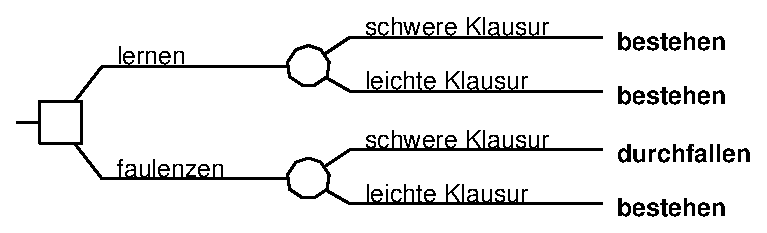
\includegraphics[width=12cm]{Grafiken/Beispiel1_1.eps}
\end{center}

Entscheidungsbäume bestehen immer aus Knoten und Ästen.
\marginline{Entscheidungs\-knoten\\~\\ und\\~\\
  Möglich\-keits\-knoten} Dabei werden die\-jenigen Knoten, an denen
eine Entscheidung zwischen unterschiedlichen Handlungsalternativen
getroffen werden muss, {\em Entscheidungs\-knoten}
genannt. Entscheidungsknoten werden durch ein Quadrat
symbolisiert. Diejenigen Knoten, die ein Zufallsereigniss
repräsentieren, werden {\em Möglichkeits\-knoten} genannt und durch
einen Kreis symbolisiert. Eingangs wurde statt von
"`Zufallsereignissen"' von "`Zuständen"' gesprochen. Die Zweige, die
auf einen Entscheidungsknoten folgen, stellen dabei unterschiedliche
"`Handlungsalternativen"' dar, zwischen denen die Entscheiderin wählen
kann.  Die Zweige, die auf einen Möglichkeitsknoten folgen,
entsprechen dagegen unterschiedlichen (Welt)-"'Zuständen"', von denen
entweder nicht sicher ist, welcher davon eintreten wird, oder von
denen wir nicht wissen welcher eintreten wird oder bereits eingetreten
ist, so dass es sich aus Sicht des Entscheiders immer noch um ein
zufälliges Ereignis handelt. (Die Unterscheidung zwischen
epistemischer Unsicherheit und objektiver Unbestimmtheit und, damit
einhergehend, die zwischen subjektiver und objektiver
Wahrscheinlichkeit muss uns an dieser Stelle noch nicht
interessieren.) Die Ergebnisse stehen am Ende der Äste.

\marginline{Umwandlung von Tabellen in Bäume} Hat man eine
Entscheidungssituation, wie in diesem Fall, bereits durch eine
Entscheidungstabelle dargestellt, dann kann man daraus sehr einfach
einen Entscheidungsbaum ableiten, der dieselbe Entscheidungssituation
wiedergibt: Man beginnt mit einem viereckigen Entscheidungsknoten. An
diesen Entscheidungsknoten hängt man alle Handlungsalternativen an,
die in der ersten Spalte der Tabelle stehen. Jeder dieser Zweige wird
dann mit einem runden Möglichkeitsknoten versehen, an den wiederum
alle Zustände angehängt werden, die in der ersten Zeile der Tabelle
stehen. Am Ende der Zweige wird dann das jeweilige Ergebnis aus der
Tabelle eingetragen.

Entscheidungsbäume haben gegenüber Entscheidungstabllen den Vorteil
größerer Anschaulichkeit. Umgekehrt erlauben Tabellen eine kompaktere
Darstellung. Die größere Anschaulichkeit soll an einem weiteren
Beispiel demonstriert werden.  Bei diesem Beispiel geht es um eine
Person, die vor der Entscheidung steht, ob sie an einem Sonntag bei
unsicherer Wetterprognose zur Küste fahren und sich dort entweder
sonnen oder, falls es regnet, dort angeln gehen würde. Die
Entscheidungssituation, die mehrere Einzelentscheidungen beinhaltet
(1) zur Küste fahren oder nicht, 2) bei Regen: Angeln gehen oder
gleich heimkehren) könnte folgendermaßen aussehen:

\begin{center}
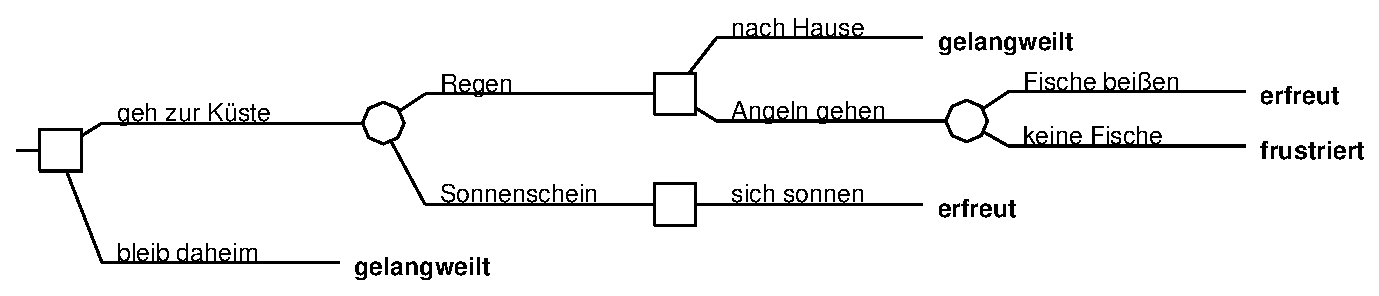
\includegraphics[width=12cm]{Grafiken/Beispiel1_2.eps}
\end{center}
(Beispiel aus \cite[S. 18]{resnik:1987})

Entscheidungsbäume erlauben es komplexe Entscheidungen, die aus
mehreren Einzelentscheidungen zusammengesetzt sind, in ihrem Verlauf
darzustellen.  Dennnoch kann man jedes Entscheidungsproblem, dass sich
durch einen Entscheidungsbaum beschreiben lässt auch als
Entscheidungstabelle darstellen.  Dazu muss man die möglichen
Sequenzen von Einzelentscheidungen zu {\em Gesamtstrategien}
zusammenfassen. Solche Gesamtstrategien müssen die "`unter allen
möglichen Eventualitäten"' zu treffenden Einzelentscheidungen
festlegen.  Gleichfalls ist es meist erforderlich, die
Zufallsereignisse zu komplexeren Zuständen zusammenzufassen. Verfährt
man in dieser Weise, dann entsteht aus dem eben präsentierten
Entscheidungsbaum folgende Tabelle:

\begin{center}
\label{AngelnBeispiel}
\begin{tabular}{c|c|c|c|}
\multicolumn{1}{c}{}  & \multicolumn{1}{c}{Regen und Fische beißen}  & \multicolumn{1}{c}{Regen und keine Fische}  & \multicolumn{1}{c}{Sonnenschein} \\ \cline{2-4}
 A1 & gelangweilt & gelangweilt & erfreut \\ \cline{2-4}
 A2 & erfreut & frustriert & erfreut \\ \cline{2-4}
 A3 & gelangweilt & gelangweilt & gelangweilt \\ \cline{2-4}
\end{tabular}
\begin{itemize}
\item {\em A1}: geh zur Küste;  wenn Regen dann nach Hause,  sonst wenn Sonnenschein dann sich sonnen

\item {\em A2}: geh zur Küste;  wenn Regen dann Angeln gehen,  sonst wenn Sonnenschein dann sich sonnen

\item {\em A3}: bleib daheim

\end{itemize}

\end{center}

\begin{quotation}
\begin{small}
{\em Quizfrage: Kann man anhand dieser Entscheidungstabelle 
 bereits feststellen, welche 
Handlungsalternative gewählt werden
sollte oder zumindest sagen, ob eine bestimmte
Handlungsalternative definitiv nicht gewählt werden sollte?}
\end{small}
\end{quotation}

Nehmen Sie sich ruhig ein wenig Zeit, um sich klar zu machen, dass die
Tabelle dem Entscheidungsbaum entspricht, d.h. dass alle
Handlungsalternativen, die nach der Baumdarstellung gewählt werden
können, auch nach der Tabellendarstellung möglich sind, und ebenso
auch alle denkbaren Kombinationen von Zufallsereignissen. Man könnte
sich dabei zunächst wundern, warum beispielsweise die Kombination der
Ereignisse "`Sonnenschein"' und "`Fische beißen"' nicht in der Tabelle
vorkommt. Aber da in dem Fall, dass die Sonne scheint, der zweite
Möglichkeitsknoten gar nicht mehr erreicht wird, wirkt sich der
Unterschied, ob die Fische beißen oder nicht, auch nicht auf das
Ergebnis aus. Insofern können beide Fälle durch ein- und dieselbe
Zustandsspalte "`Sonnenschein"' erfasst werden

Das Verfahren, wie man einen Entscheidungsbaum in eine Tabelle
überführt, ist ebenfalls rein mechanischer Art. Da es etwas
komplizierter ist als die Umwandlung einer Tabelle in einen
Entscheidungsbaum, werden wir es gleich (Abschnitt \ref{BaumTabelle})
ausführlicher betrachten. Bis dahin soll einfach als gegeben
angenommen werden, dass dies immer möglich ist.

% Die Einzelheiten dieses Verfahrens, das intuitiv sehr
% viel leichter zu erfassen als exakt zu beschreiben ist, müssen uns an dieser
% Stelle nicht interessieren. Ebenso soll an dieser Stelle der Beweis, dass sich
% jeder Entscheidungsbaum in eine Tabelle, die dasselbe Entscheidungsproblem
% ausdrückt, überführen lässt, übergangen werden. (Der Beweis besteht im
% wesentlichen darin, ein Verfahren zur Transformation eines Entscheidungsbaums
% in eine Tabelle anzugeben. Dieser Beweis erfordert keine besonders originellen
% Ideen. Die Kunst besteht jedoch darin, das entsprechende Verfahren exakt zu
% beschreiben; so exakt, dass man es in einen Computer einprogrammieren könnte.
% Wer möchte kann sich ja mal daran versuchen ;) )

Wenn wir es aber einmal als gegeben betrachten, dass man jeden
Entscheidungsbaum in eine Entscheidungstabelle überführen kann, und,
wie zuvor schon gezeigt wurde, jede Entscheidugnstabelle in einen
Entscheidungsbaum, dann hat das die für uns wichtige Konsequenz, dass
wir frei sind, uns je nach Konvenienz der einen oder der anderen
Darstellung zu bedienen. Dies gilt insbesondere für die Entwicklung
der Entscheidungstheorie selbst. Denn wir können nun davon ausgehen,
dass alle Überlegungen, die wir in Bezug auf Entscheidungsprobleme
anhand einer der Darstellungsformen anstellen, ihre Gültigkeit
behalten, wenn wir zu der anderen Darstellungsform übergehen. Für die
Entwicklung der Theorie eignet sich dabei die kompaktere Tabellenform
häufig besser. Umgekehrt bietet sich für die Darstellung und Lösung
bestimmter Entscheidungsprobleme oft eher die anschaulichere
Darstellung durch Entscheidungsbäume eher an.

Wenn die Rede davon war, dass sich Tabellendarstellung und
Baumdarstellung auf mechanische Weise ineinander überführen lassen, so
bedeutet das allerdings nicht, dass wenn man nach diesem Verfahren
einen Entscheidungsbaum zuerst in eine Tabelle und dann wieder in
einen Baum überführt, auch derselbe Entscheidungsbaum wieder dabei
heraus kommt. Transformiert man die eben gewonnene Tabelle wieder in
einen Baum, so hat dieser Entscheidungsbaum die folgende Gestalt:

\begin{center}
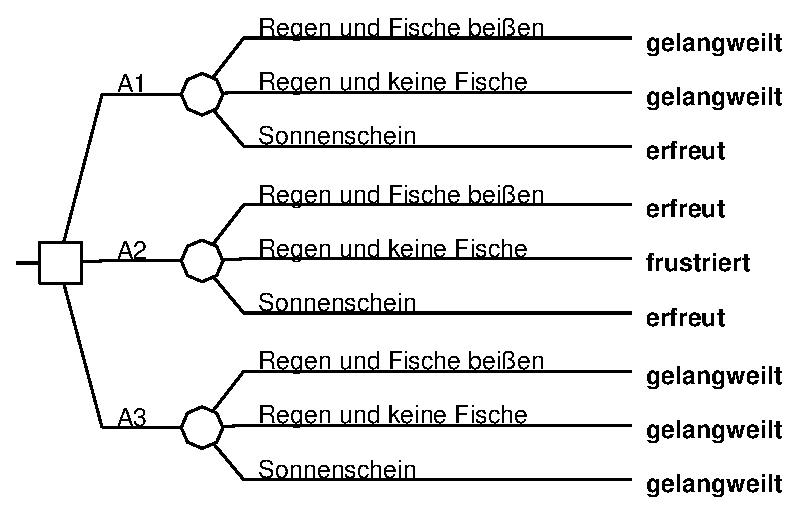
\includegraphics[width=12cm]{Grafiken/Beispiel1_4.eps}
\end{center}

Dass der Entscheidungsbaum nach der Übertragung in die Tabellenform und dann
wieder der Rückübertragung in die Baumform ganz anders aussieht, sollte
allerdings nicht verwundern, denn es gibt in der Regel viele unterschiedliche 
Möglichkeiten ein- und dasselbe Entscheidungsproblem als Baum- und Tabelle
darzustellen. Der zuletzt gezeigte Baum stellt in der Tat dasselbe
Entscheidungsproblem dar wie der ursprüngliche Baum. Identisch sind zwei
Entscheidungsprobleme genau dann, wenn denselben Kombinationen von
Handlungsalternativen und Zuständen dieselben Ergebnisse zugeordnet sind. Bei
Entscheidungen unter Risiko müssen die möglichen Weltzustände darüber hinaus
mit denselben Wahrscheinlichkeiten eintreten. Leider kann man weder der
Baumdarstellung noch der Tabellendarstellung unmittelbar ansehen, ob zwei
Entscheidungsprobleme identisch sind. Für die Entscheidungsbäume ist dies nach
dem vorhergehenden Beispiel offensichtlich. Bei Tabellen ergibt sich dies unter
anderem daraus, dass die Reihenfolge der Spalten und Zeilen für das zu Grunde
liegende Entscheidungsproblem egal ist (siehe Aufgabe
\ref{ZeilenSpaltenPermutation}).


\subsubsection{Exkurs: Entscheidungsbäume in Tabellen umwandeln}
\label{BaumTabelle}

{\em Dieses Teilkapitel ist als Exkurs gedacht. Wem es für den Anfang zu
schwierig ist, der kann diesen Exkurs (und die dazu gehörigen Übungsaufgaben) 
ruhig überspringen. Im Folgenden wird darauf nicht mehr zurück gegriffen.}

Um Entscheidungsbäume in Tabellen umzuwandeln, können wir uns den
Umstand zu Nutze machen, dass Entscheidungsbäume, so kompliziert sie
auch sein mögen, aus der Kombination von nur zwei Elementen bestehen,
Entscheidungsknoten und Zufallsknoten. Um einen Entscheidungsbaum in
eine Tabelle zu überführen müssen wir also nur wissen, wie man 1)
Entscheidungsknoten in eine Tabelle überträgt, wie man 2)
Zufallsknoten in eine Tabelle überträgt und 3) wie man einen
komplizierten zusammengesetzten Baum schrittweise mit Hilfe der beiden
vorherigen Übertragungsregeln reduziert.

1) Ein Entscheidungsbaum, der nur aus einem einzigen Ent\-scheidungs\-knoten mit
zwei Alternativen besteht, ergibt eine Tabelle mit zwei Zeilen und einer Spalte:

\vspace{0.5cm}

\parbox{7cm}{Baum:}\parbox{5cm}{Tabelle:}

\vspace{0.25cm}

\parbox{7cm}{
\includegraphics[width=6cm]{Grafiken/Beispiel1b_1.eps}}
\parbox{5cm}{
\begin{tabular}{c|c|}
      & $S_1$ \\ \cline{1-2}
$A_1$ & $r_1$ \\ \cline{1-2}
$A_2$ & $r_2$ \\ \cline{1-2}
\end{tabular}}

\vspace{0.5cm}

2) Ein Baum, der nur aus einem Zufallsknoten besteht, liefert demgegenüber eine
Tabelle mit nur einer Zeile und genau soviel Spalten wie Ereignisse an dem
entsprechenden Ereignisknoten eintreten können.

\vspace{0.5cm}

\parbox{7cm}{Baum:}\parbox{5cm}{Tabelle:}

\vspace{0.25cm}

\parbox{7cm}{\includegraphics[width=6cm]{Grafiken/Beispiel1b_2.eps}}
\parbox{5cm}{
\begin{tabular}{c|c|c|}
      & $S_1$ & $S_2$ \\ \cline{1-3}
$A_1$ & $r_1$ & $r_2$ \\ \cline{1-3}
\end{tabular}}

\vspace{0.5cm}

3) Wie kann man nun aber einen Entscheidungsbaum, der aus einer
Vielzahl von Entscheidungs- und Zufallsknoten besteht, in eine Tabelle
überführen? Dazu wird der Baum schrittweise von hinten
"`aufgerollt"'. Die jeweils "`letzten"' Entscheidungs-
bzw. Zufallsknoten von rechts entsprechen genau den vorher
beschriebenen Fällen und können auf die beschriebende Weise
umgewandelt werden.  Kompliziert wird es erst bei den weiter in der
Mitte und am Anfang liegenden Knoten. Wenn wir an einem solchen Knoten
ankommen, haben wir den Baum aber schon soweit aufgerollt, dass wir zu
den sich an den Knoten anschließenden Teilbäumen bereits über Tabellen
verfügen. Das Problem stellt sich also folgendermaßen dar: Wie kann
ein Entscheidungsknoten bzw. ein Zufallsknoten in eine Tabelle
überführt werden, an dessen Enden sich wiederum ganze
Entscheidungsbäume anschließen, für die wir aber immerhin schon über
eine Repräsentation in Tabellenform verfügen?

Um dieses Problem zu lösen, müssen wir wiederum Entscheidungs- und
Zufallsknoten getrennt betrachten:

3 a) Angenommen, wir haben es mit einem Entscheidungsknoten zu tun. Dann endet
der Entscheidungsknoten in zwei Teilbäumen, die bereits als Tabellen
dargestellt sind. Jede dieser Tabellen enthält wiederum eine Menge von
Handlungsalternativen und eine Menge von Zufallsereignissen.

\vspace{0.5cm}

\begin{small}
\parbox{3.5cm}{\ }
\parbox{4.5cm}{\begin{center}Tabelle zu Baum 1\end{center}}
\parbox{4.5cm}{\begin{center}Tabelle zu Baum 2\end{center}}

\parbox{3.5cm}{
\includegraphics[width=3.5cm]{Grafiken/Beispiel1b_3.eps}}
\parbox{4.5cm}{
\begin{tabular}{c|ccc|}
         & $S_1$    & $\cdots$ & $S_n$     \\ \cline{1-4}
$A_1$    & $r_{11}$ & $\cdots$ & $r_{1n}$  \\ %\cline{1-4}
$\vdots$ & $\vdots$ & $\ddots$ & $\vdots$  \\ %\cline{1-4}
$A_m$    & $r_{m1}$ & $\cdots$ & $r_{mn}$  \\ \cline{1-4}
\end{tabular}}
\parbox{4.5cm}{
\begin{tabular}{c|ccc|}
         & $T_1$    & $\cdots$ & $T_l$     \\ \cline{1-4}
$B_1$    & $u_{11}$ & $\cdots$ & $u_{1l}$  \\ %\cline{1-4}
$\vdots$ & $\vdots$ & $\ddots$ & $\vdots$  \\ %\cline{1-4}
$B_h$    & $u_{h1}$ & $\cdots$ & $u_{hl}$  \\ \cline{1-4}
\end{tabular}}
\end{small}

\vspace{0.5cm}

Die beiden Ereignismengen $\{S_1, \ldots, S_n\}$ und $\{T_1, \ldots, T_l\}$ des
ersten und des zweiten Teilbaums sowie die entsprechenden Mengen von
Handlungsalternativen $\{A_1, \ldots, A_m\}$ und $\{B_1, \ldots, B_h\}$ müssen
nun in geeigneter Form kobminiert werden, um die Tabelle des gesamten
Entscheidungsknotens aufzubauen. Das geschieht folgendermaßen: In den Spalten
der zusammengefassten Tabelle muss jede mögliche Kombination der
Zufallsereignisse aus beiden Mengen eingetragen werden. In den Zeilen wird als
erstes der Block von Handlungen $X_1 \wedge A_1,\ldots, X_1 \wedge A_m$
eingetragen, worauf als zweites ein Block von Handlungen $X_2 \wedge
B_1,\ldots, X_2 \wedge B_h$ folgt (d.h. jede der Handlungen der ersten Tabelle
wird mit der Handlung $X_1$ kombiniert, jede alternative Handlung der zweiten
Tabelle mit $X_2$).\footnote{Das aus der Logik bekannte Zeichen $\wedge$
bedeutet "`und"', so dass der Ausdruck $X_1 \wedge A_1$ so zu verstehen ist,
dass die Handlung $X_1$ {\em und} die (möglicherweise wiederum aus mehreren
Einzelhandlungen zusammengesetzte) Handlung $A_1$ ausgeführt werden.} Daraus
ergibt sich folgende kombinierte Tabelle:

\begin{small}
\begin{center}
\begin{tabular}{c|ccc|c|ccc|}
                 & $S_1 \wedge T_1$  & $\cdots$ & $S_n \wedge T_1$ & $\cdots$
                 & $S_1 \wedge T_l$  & $\cdots$ & $S_n \wedge T_l$  
                 \\ \cline{1-8} 
$X_1 \wedge A_1$ & $r_{11}$          & $\cdots$ & $r_{1n}$ & $\cdots$ 
                 & $r_{11}$          & $\cdots$ & $r_{1n}$  \\
  $\vdots$       & $\vdots$          & $\ddots$ & $\vdots$ & $\ddots$
                 & $\vdots$          & $\ddots$ & $\vdots$\\
$X_1 \wedge A_m$ & $r_{m1}$          & $\cdots$ & $r_{mn}$ & $\cdots$
                 & $r_{m1}$          & $\cdots$ & $r_{mn}$\\ \cline{1-8}
                   
$X_2 \wedge B_1$ & $u_{11}$          & $\cdots$ & $u_{11}$ & $\cdots$
                 & $u_{1l}$          & $\cdots$ & $u_{1l}$\\
  $\vdots$       & $\vdots$          & $\ddots$ & $\vdots$ & $\ddots$
                 & $\vdots$          & $\ddots$ & $\vdots$\\                  
$X_2 \wedge B_h$ & $u_{h1}$          & $\cdots$ & $u_{h1}$ & $\cdots$
                 & $u_{hl}$          & $\cdots$ & $u_{hl}$\\\cline{1-8}
\end{tabular}
\end{center}
\end{small}

Man beachte: Jedes mögliche Resultat $r_{xy}$ aus der ersten Tabelle kommt genau
$l$-mal vor, d.h. genauso viel mal, wie es Zufallsereignisse in der zweiten
Tabelle gibt. Umgekehrt kommt jedes mögliche Resultat $u_{xy}$ aus der zweiten Tabelle
genau $n$-mal vor, wobei $n$ die Anzahl der Zufallsereignisse in der
ersten Tabelle ist. (Die entsprechende Tabellendarstellung ist also in
der Regel hochgradig redundant und könnte, wenn dies der Fall ist, nachträglich
noch vereinfacht werden.)

\vspace{0.5cm}

3 b) Geht es statt dessen um die Umwandlung eines Zufallsknotens, dann stehen
wir vor der spiegelbildlichen Situation, so dass wir diesmal zwei Spaltenblöcke
bilden und in den Zeilen jede Kombination möglicher Handlungen zu
berücksichtigen haben. 

\vspace{0.5cm}

\begin{small}
\parbox{3.5cm}{\ }
\parbox{4.5cm}{\begin{center}Tabelle zu Baum 1\end{center}}
\parbox{4.5cm}{\begin{center}Tabelle zu Baum 2\end{center}}

\parbox{3.5cm}{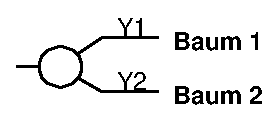
\includegraphics[width=3.5cm]{Grafiken/Beispiel1b_4.eps}}
\parbox{4.5cm}{
\begin{tabular}{c|ccc|}
         & $S_1$    & $\cdots$ & $S_n$     \\ \cline{1-4}
$A_1$    & $r_{11}$ & $\cdots$ & $r_{1n}$  \\ %\cline{1-4}
$\vdots$ & $\vdots$ & $\ddots$ & $\vdots$  \\ %\cline{1-4}
$A_m$    & $r_{m1}$ & $\cdots$ & $r_{mn}$  \\ \cline{1-4}
\end{tabular}}
\parbox{4.5cm}{
\begin{tabular}{c|ccc|}
         & $T_1$    & $\cdots$ & $T_l$     \\ \cline{1-4}
$B_1$    & $u_{11}$ & $\cdots$ & $u_{1l}$  \\ %\cline{1-4}
$\vdots$ & $\vdots$ & $\ddots$ & $\vdots$  \\ %\cline{1-4}
$B_h$    & $u_{h1}$ & $\cdots$ & $u_{hl}$  \\ \cline{1-4}
\end{tabular}}
\end{small}

\vspace{0.5cm}

Um die kombinierte Tabelle zu konstruieren, müssen wir also zwei Spaltenblöcke
bilden, wobei der erste Block alle Zufallsereignisse der ersten Tabelle umfasst
(und-verknüpft mit dem Ereignis $Y_1$ versteht sich!) und der zweite Block die
der zweiten Tabelle: In den Zeilen treten alle Kombinationen möglicher
Handlungen auf, und zwar, da die Möglichkeit, eine bestimmte Handlung zu
wählen oder nicht zu wählen erst durch das Eintreten von $Y_1$ oder $Y_2$
überhaupt eröffnet wird, in einer "`wenn\ldots, dann\ldots"'-Form. In einer 
abgekürzten Schreibweise, bei der das Zeichen "`$\rightarrow$"' für die 
wenn-dann-Beziehung stehen soll, schreiben wir also z.B.
$(Y_1 \rightarrow A_2) \wedge (Y_2 \rightarrow B_5)$.\footnote{Angesichts der 
Symmetrie zwischen dem Problem der Umwandlung eines Entscheidungsknotens 
in eine Tabelle und dem der Umwandlung eines
Zufallsknotens in eine Tabelle, könnte es verwundern, dass wir im zweiten Fall
in den Zeilen der generierten Tabelle "`wenn\ldots, dann\ldots"'-Audrücke
vorfinden, während wir uns im ersteren Fall mit simpleren und-Verknüpfungen
begnügen. Dies ist dadurch motiviert, dass wir davon ausgehen, dass die
Ereignisse der Serien $T_1, \ldots, T_n$ bzw. $S_1, \ldots, S_n$ unabhängig von
den getroffenen Entscheidungen auch dann eintreten, wenn sie angesichts des gewählten Zweiges
für das erzielbare Ergebnis nicht mehr relevant sind. Diese Annahme ist
zwar harmlos aber keinesfalls zwingend. Wollte man ganz präzise sein, dann
müsste man die Spaltenüberschriften der aus einem Entscheidungsknoten gewonnen Tabelle
ebenfalls als "`wenn\ldots, dann\ldots"'-Aussagen ausformulieren.}

\begin{small}
\begin{center}
\begin{tabular}{c|ccc|ccc|}
                 & $Y_1 \wedge S_1$  & $\cdots$ & $Y_1 \wedge S_n$
                 & $Y_2 \wedge T_1$  & $\cdots$ & $Y_2 \wedge T_l$  
                 \\ \cline{1-7} 
$Y_1 \rightarrow A_1 \wedge Y_2 \rightarrow B_1$  
                 & $r_{11}$          & $\cdots$ & $r_{1n}$  
                 & $u_{11}$          & $\cdots$ & $u_{1l}$  \\
  $\vdots$       & $\vdots$          & $\ddots$ & $\vdots$ 
                 & $\vdots$          & $\ddots$ & $\vdots$\\
$Y_1 \rightarrow A_1 \wedge Y_2 \rightarrow B_h$     
                 & $r_{11}$          & $\cdots$ & $r_{1n}$ 
                 & $u_{h1}$          & $\cdots$ & $r_{hl}$\\ \cline{1-7}

  $\vdots$       & $\vdots$          & $\ddots$ & $\vdots$ 
                 & $\vdots$          & $\ddots$ & $\vdots$\\ \cline{1-7}
                   
$Y_1 \rightarrow A_m \wedge Y_2 \rightarrow B_1$  
                 & $r_{m1}$          & $\cdots$ & $r_{mn}$  
                 & $u_{11}$          & $\cdots$ & $u_{1l}$  \\
  $\vdots$       & $\vdots$          & $\ddots$ & $\vdots$ 
                 & $\vdots$          & $\ddots$ & $\vdots$\\
$Y_1 \rightarrow A_m \wedge Y_2 \rightarrow B_h$     
                 & $r_{m1}$          & $\cdots$ & $r_{mn}$ 
                 & $u_{h1}$          & $\cdots$ & $r_{hl}$\\ \cline{1-7}
\end{tabular}
\end{center}
\end{small}

Mit diesen beiden "`Übersetzungsregeln"' kann man jeden Entscheidungsbaum
systematisch schrittweise in eine Tabelle überführen. Man ahnt, dass die
Tabelle ziemlich groß werden kann. Dies hängt auch damit zusammen, dass wir an
dieser Stelle auf Sonderfallbetrachtungen verzichtet haben, die die Tabelle
vereinfachen könnten. Z.B. ist es sehr wohl möglich, dass unterschiedliche
Zufallsknoten in einem Baum in Wirklichkeit ein- und dasselbe Ereignis
ausdrücken, nur dass es je nach den zuvor getroffenen Entscheidungen
möglicherweise zu anderen Resultaten führt. Am Beispiel von vorhin lässt sich
dies erläutern:
\begin{center}
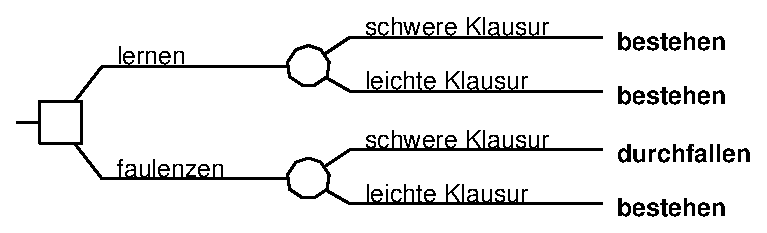
\includegraphics[width=8cm]{Grafiken/Beispiel1_1.eps}
\end{center}
Würde man diesen Entscheidungsbaum nach unserem "`mechanischen"' Verfahren in
eine Tabelle überführen, dann würden in den Spaltenüberschriften die Ereignisse
"`schwere Klausur \& schwere Klausur"', "`schwere Klausur \& leichte Klausur"',
"`leichte Klausur \& schwere Klausur"' und "`leichte Klausur \& leichte
Klausur"' stehen. Das hängt damit zusammen, dass der Algorithmus zunächst keine
Informationen darüber hat, ob unterschiedliche Zufallsknoten möglicherweise
identische Zufallsereignisse repräsentieren. Man müsste den
Entscheidungsbaum um entsprechende Informationen ergänzen (z.B. indem man eine
Verbindungslinie zwischen identischen Ereignissen zieht) und den Algorithmus so
anpassen, dass er unmögliche Ereigniskombinationen ("`schwere \& leichte
Klausur"') streicht. 

Weiterhin haben wir den Algorithmus zur Übersetzung von Bäumen in Tabellen
zunächst nur für {\em Binär-}bäume (d.h. Bäume, die an jeder Verzweigung nur
zwei Äste haben) beschrieben. Das ist aber unproblematisch, da man jeden
Entscheidungsbaum in einen binären Entscheidungsbaum umwandeln kann. Z.B. kann
der Entscheidungsbaum
\begin{center}
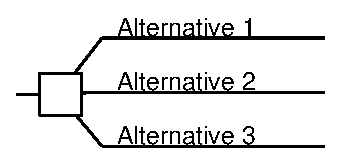
\includegraphics[width=5cm]{Grafiken/Beispiel1b_5.eps}
\end{center}
einfach in den Baum
\begin{center}
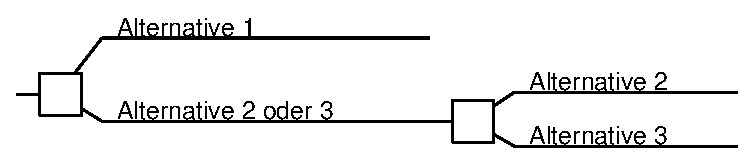
\includegraphics[width=10cm]{Grafiken/Beispiel1b_6.eps}
\end{center}
umgewandelt werden. Eine andere Alternative bestünde darin, den Algorithmus so
anzupassen, dass er sich auch für nicht binäre Entscheidungsbäume eignet
(siehe  Übungsaufgabe \ref{Algorithmusaufgabe} auf Seite
\pageref{Algorithmusaufgabe}).


\subsection{Literaturhinweise}

Zum Schluss ein par Worte zu der Fachliteratur, auf die sich diese Vorlesung
stützt, und die ich als Ergänzung zu diesem Skript als Begeleittexte empfehle:
Zum überwiegenden Teil werde ich in dieser Vorlesung dem Buch "`Choices. An
Introduction to Decision Theory"' von Micheal D. \cite{resnik:1987} folgen. Es
handelt sich dabei um eine didaktisch gut aufbereitete und sehr verständliche
Einführung in die Entscheidungstheorie und die Grundlagen der Spieltheorie.
% Speziell für die Spieltheorie wird auch die Einführung von Martin J. Osborne
% "`An Introduction to Game Theory" \cite{osborne:2004} verwendet.
Für die etwas mathematischeren Teile dieser Vorlesung, insbesondere für den
"`Satz von Arrow"' und die "`Neumann-Morgensternschen Nutzenfunktionen"', möchte
ich auch auf die sehr klare und verständliche Darstellung in dem Lehrbuch von
\cite{mascolell-whinston-green:1995} verweisen. Speziell was die philosophischen
Probleme im Zusammenhang mit der Entscheidungstheorie angeht, werde ich weiterhin
Das Buch von Mark Kaplan "`Decision Theory as Philosophy"' \cite[]{kaplan:1996}
hinzuziehen. Für die Themen aus dem Bereich Social Choice und Public Choicde, 
greife ich unter anderem auf Dennis C. Mueller: "`Public Choice III"'
\cite[]{mueller:2003} zurück. (Als kritische Ergänzung zu der sehr einseitigen
Darstellung Muellers ist, wie bereits erwähnt, das Buch "`The Pathologies of
Rational Choice"' von \cite{green-shapiro:1994}
sehr empfehlenswert.) Soweit in der Vorlesung auch wissenschaftstheoretische Fragen
berührt werden, beziehe ich mich hauptsächlich auf Gerhard Schurz' "`Einführung
in die Wissenschaftstheorie"' \cite[]{schurz:2006}.


\newpage
\subsection{Aufgaben}

\begin{enumerate}
  \item {\em Stelle folgendes Ent\-scheidungs\-problem als
  Ent\-scheidungs\-baum dar}: Paula und Fritz stoßen an einer vielbefahrenen
  Kreuzung mit ihren Autos zusammen. Vieles spricht dafür, dass Fritz schuld ist. Deshalb bietet Fritz'
  Versicherung Paula € 5.000 als Schadensersatz und Schmerzensgeld an.
  Paula glaubt jedoch, dass ihr mehr zusteht und überlegt vor Gericht
  zu ziehen. Wenn Sie klagt, dann könnte es sein, dass Fritz' Versicherung ihr
  Angebot im Falle einer außergerichtlichen Einigung auf € 10.000 erhöht. Es ist
  aber auch möglich, dass die Versicherung ihr ursprüngliches Angebot
  beibehält. Gewinnt Paula den Prozess, dann erhält sie € 20.000. Verliert Sie
  den Prozess, dann bekommt sie gar nichts. (Gerichts- und Anwaltskosten können
  zunächst vernachlässigt werden.)

  \item {\em Aufgabe}: Angenommen, bei einer Klage, die später zurückgezogen
  wird, fallen für die Klägerin immer noch Anwalts- und Gerichtskosten von €
 500 an. Angenommen weiterhin, der Prozess kostet den Verlierer oder die
 Verliererin € 2.500. {\em Wie sieht nun der Entscheidungsbaum aus?}

 \item Stelle das Entscheidungsproblem aus der vorhergehenden Aufgabe als
 Tabelle dar.

 \item {\em Aufgabe}: Angenommen, Paula würde eine
  Klage gar nicht erst in Erwägung ziehen, wenn die Versicherung von Fritz ihr
  gleich € 10.000 anbietet und sie würde ihre Klage wieder fallen lassen, wenn
  sich die Versicherung außergerichtlich auf € 15.000 mit ihr einigt. Für die
  Prozesskosten der Versicherung soll dasselbe gelten wie in Aufgabe 2. {\em Wie
  sieht der Entscheidungsbaum aus Sicht der Versicherung aus?}

 \item \label{ZeilenSpaltenPermutation} {\em Erkläre:} Wenn man bei einer
 Enscheidungstabelle beliebig oft ganz Spalten oder ganze Zeilen vertauscht,
 stellt sie immer noch ein- und dasselbe Entscheidungsproblem dar. Warum?
% \item  {\em Aufgabe zur Wahrscheinlichkeitsrechnung}: Auf einer
% Geburtstagsfeier treffen 40 Gäste ein. a) Wie groß ist die Wahrscheinlichkeit,
% dass sich unter den Gästen mindestens eine Person befindet, die am selben Tag
% Geburtstag hat, wie das "`Geburtstagskind"'? b) Ab welcher Anzahl von geladenen
% Gästen würde die Wahrscheinlichkeit mehr als 50\% betragen?


  ~\\ {\bf Schwerere Aufgaben:}\\
 
 \item \label{Algorithmusaufgabe} Formuliere den Algorithmus zur Umwandlung von
 Entscheidungsbäumen in Entscheidungstabellen (siehe Abschnitt \ref{BaumTabelle}) so um, dass er auch
 für nicht binäre Entscheidungsbäume geeignet ist.
 
 \item Beweise (bzw. Erläutere), dass die Kombinationen von Zufallsereignissen
 in den durch den Algorithmus zur Umwandlung von Entscheidungsbäumen 
(siehe Abschnitt \ref{BaumTabelle}) generierten Tabellen immer noch
wechselseitig ausschließend und zugleich erschöpfend (d.h. eins der Ereignisse tritt auf jeden Fall ein) sind.
 
%  \item {\em Aufgabe zur Mengenlehre}: Unter einer {\em abzählbar unendlich}
%  großen Menge versteht man eine Menge, die sich bijektiv ("`ein-eindeutig"')
%  auf die Menge der natürlichen Zahlen abbilden lässt. Das
%  {\em kartesische Produkt} zweier Mengen A und B ist definiert als die Menge
%  aller Tupel $(a, b)$ mit $a \in A$ und $b \in B$. {\em Zeige: Das kartesische
%  Produkt zweier abzählbar unendlicher Mengen ist wieder abzählbar unendlich.} 
\end{enumerate}

% \subsection{Zusatzaufgaben}
% 
% \begin{enumerate}
%  \item Eine Ölfirma erwägt an einer bestimmten Stelle in der Nordsee nach Öl zu
%  bohren. Es ist nicht absolut sicher, ob sich an dem entsprechenden Ort
%  tatsächlich Öl befindet. Um dies mit Sicherheit festzustellen, kann die Firma
%  eine Probebohrung durchführen lassen. Der Bau einer Bohrinsel
%  kostet € 1.000.000. Liefert die Bohrinsel tatsächlich Öl, so gewinnt die
%  Ölfirma abzüglich der Betriebskosten € 10.000.000. Die Durchführung einer
%  Probebohrung kostet € 250.000. {\em Zeichne den Entscheidungsbaum und die
%  Entscheidungstabelle} (Zur Diskussion: Sollte die Firma in jedem Fall eine
%  Probebohrung durchführen?)
% \end{enumerate}

\newpage
 
\newpage
\section{Entscheidungen unter Unwissenheit I}

In dieser und der folgenden Woche werden wir uns mit Entscheidungen unter
Unwissen beschäftigen. Entscheidungen unter Unwissen sind
Entscheidungen, bei denen wir nicht wissen mit welcher Wahrscheinlichkeit
bestimmte Ereignisse (bzw. "`Welt-Zustände"') eintreten können, bei denen wir
aber immer noch eine klare Vorstellung davon haben, mit welchen Ereignissen
als Bedingungen unserer Entscheidungen und mit welchen Ergebnissen als
Resultaten der Entscheidungen überhaupt zu rechnen ist. Entscheidungen unter
Unwissen sind zu unterscheiden von Entscheidungen unter "`vollständiger
Unwissenheit"' einerseits, bei denen wir nicht einmal mehr mit Sicherheit
angeben können, zu welchen möglichen Resultaten unsere Handlungen führen
können, und von "`Entscheidungen unter Risiko"' andererseits, bei denen wir
zusätzlich Aussagen über Wahrscheinlichkeit der in Betracht zu ziehenden
Ereignisse machen können. 

Naturgemäß bieten Entscheidungen unter Risiko, bei denen wir
Wahr\-schein\-lich\-keiten angeben können, die besten Angriffspunkte für eine
formale Theorie des Entscheidens. Aber auch Entscheidungen unter Unwissenheit
sind bis zu einem gewissen Grade einer formalen Behandlung zugänglich, und weil
dabei die Wahrscheinlichkeitstheorie nicht erforderlich ist, handelt es sich
technisch gesehen sogar um den einfacheren Teil der Entscheidungstheorie, weshalb
wir diesen Teil auch zuerst besprechen.

\subsection{Die einfachste Entscheidungsregel: Das Prinzip der Dominanz}
\label{DominanzPrinzip}
Bisher haben wir nur über die Darstellung von Entscheidungsproblemen in Form von
Entscheidungsbäumen und -tabellen gesprochen. Wie kann man aber nun (mit Hilfe
von Bäumen oder Tabellen) Entscheidungsprobleme lösen? Ein besonders
offensichtliches Prinzip, das bei der Lösung von Entscheidungsproblemen eine
Rolle spielt, ist das {\em Prinzip der Dominanz}. Betrachten wir dazu noch
einmal die eingangs vorgestellte Entscheidungstabelle:

\begin{center}
\begin{tabular}{cc|c|c|}
& \multicolumn{1}{c}{} & \multicolumn{2}{c}{{\bf Zustand}} \\
&           & schwere Klausur   & leichte Klausur    \\ \cline{2-4}
& lernen    & {\em bestehen}    &  {\em bestehen}    \\ \cline{2-4}
\raisebox{1.5ex}[-1.5ex]{{\bf Handlung}} 
& faulenzen & {\em durchfallen} &  {\em bestehen} \\
\cline{2-4}
\end{tabular}
\end{center}

Man sieht anhand der Tabelle sofort, dass es auf jeden Fall besser wäre zu
lernen als zu faulenzen, denn in dem Fall, dass die Klausur schwer ist,
erzielt man durch Lernen ein besseres Ergebnis und in dem Fall, dass sie leicht
wird, ist das Ergebnis wenigstens nicht schlechter als wenn man nicht lernt.
Das bei dieser Überlegung implizit zu Grunde gelegte Entscheidungsprinzip kann
man folgendermaßen formulieren.

\begin{quotation}
\marginline{schwache Dominanz}
{\em Prinzip der schwachen Dominanz}: Wenn eine Handlung unter
allen Umständen zu einem mindestens gleichguten Ergebnis führt wie alle anderen
Alternativen und in mindestens einem möglichen Fall zu einem besseren Ergebnis,
dann wähle diese Handlung.
\end{quotation}

\marginline{starke Dominanz}
Analog zu dem Prinzip der schwachen Dominanz kann man auch ein Prinzip der
starken Dominanz aufstellen, bei dem gefordert wird, dass die zu wählende
Handlung unter allen Umständen zu einem eindeutig besseren Ergebnis führt als
sämtliche verfügbaren Alternativen. An dieser Stelle ist die Unterscheidung
zwischen schwacher Dominanz und starker Dominanz noch nicht besonders
wichtig. Der Begriff der starken Dominanz könnte sogar verzichtbar
erscheinen. Allerdings spielt diese Unterscheidung spätestens bei der Suche nach
geeigneten Lösungsstrategien in der Spieltheorie wieder eine wichtige Rolle und
wird uns dort noch beschäftigen.

\marginline{Mögliche Fehlschlüsse}
Das Prinzip der schwachen Dominanz erscheint so einfach und eindeutig, dass man
nicht vermuten sollte, dass es bei seiner Anwendung irgendwelche
Schwierigkeiten auftreten könnten. Dass das nicht unbedingt stimmen muss, kann
das folgende Beispiel verdeutlichen: Angenommen, Sie betreten ein Wettbüro, in
dem Sportwetten für die Sportarten Fussball und Tennis angeboten werden. Der
Einsatz beträgt in jedem Fall 2 Euro, aber da sehr viel weniger Leute an
Tennis interessiert sind als an Fussball, können Sie bei einer Tenniswette
höchstens € 10.000 gewinnen, während bei einer Fußballwette satte 
€ 50.000 drin sind. Ihre Entscheidungstabelle würde als folgendermaßen
aussehen:

\begin{center}
\begin{tabular}{c|c|c|}
\multicolumn{1}{c}{ } & \multicolumn{1}{c}{Wette gewinnt} &
\multicolumn{1}{c}{Wette verliert} \\ \cline{2-3}
Tenniswette   & €  9.998    & € -2         \\ \cline{2-3}
Fussballwette & € 49.998    & € -2         \\ \cline{2-3}
\end{tabular}
\end{center}

Wollte man in dieser Situation auf das Prinzip der Dominanz zurückgreifen, dann
müsste man sich eigentlich ganz klar für die Fussballwette entscheiden. Warum
könnte das aber ein Trugschluss sein? Der Grund ist folgender: Es ist höchst
wahrscheinlich, dass die Gewinnchancen bei beiden Wetten sehr unterschiedlich
verteilt sind. Werden einem zwei solche Wetten angeboten, dann ist davon
auszugehen, dass die Gewinnchancen bei der Fussballwette sehr viel geringer
sind als bei der Tenniswette. Je nachdem, um wieviel sie geringer sind, könnte
es sein, dass die Tenniswette sogar aussichtsreicher ist als die Fussballwette.
(Was "`aussichtsreicher"' dabei exakt heisst, werden wir noch genau definieren,
wenn wir Entscheidungen unter Risiko besprechen.) Wenn man so will, besteht der
"`Denkfehler"' bei diesem Beispiel also darin, dass die Problemspezifikation
unvollkommen war, indem wichtige Hintergrundinformationen über die Natur dieses
speziellen Entscheidungsproblem, \marginline{Handlungs\-ab\-hängige
Wahr\-schein\-lich\-keiten} nämlich die Handlungs\-abhängigkeit der
Eintrittswahrscheinlichkeiten der Ereignisse, bei der Formalisierung in
Tabellenform "`vergessen"' wurden.

% An diesem Beispiel wird zugleich deutlich, dass das Prinzip der Dominanz nur
% dann sinnvoll angewandt werden kann, wenn die Chancen für das Eintreten der
% Zufallsereignisse entweder gleichverteilt sind, oder wenn wir zumindest
% keinerlei Wissen darüber haben, wie sie verteilt sein könnten.\footnote{Die
% Anwendung des Dominanzprinzips im letzteren Fall ist aber umstritten. Siehe dazu auch,
% was weiter unten zum "`Prinzip der Indifferenz"' (Abschnitt
% \ref{Indifferenzprinzip}) gesagt wird.}

Daneben gibt es aber noch ein weiteres denkbares Problem, wie das folgende, mit
leichten Abwandlungen aus Resniks Buch \cite[S.9 ]{resnik:1987} übernommene
Beispiel verdeutlicht. Das Beispiel gibt stark vereinfacht die strategische
Problematik der Aufrüstung im kalten Krieg wieder:

\begin{center}
\begin{tabular}{c|c|c|}
\multicolumn{1}{c}{ } & \multicolumn{1}{c}{Krieg}   & 
\multicolumn{1}{c}{Frieden}  \\ \cline{2-3} 
Aufrüsten & "`Tot"' & hohe Militärausgaben  \\ \cline{2-3} 
Abrüsten  & "`Rot"' & "`Friedensdividende"' \\ \cline{2-3}
\end{tabular}
\end{center}

Nimmt man einmal an, dass es besser ist, sich zum Kommunismus bekehren zu lassen
als zu sterben, dann müsste man nach dem Prinzip der Dominanz eigentlich
Handlungsalternative "`Abrüsten"' eindeutig vorziehen, denn unabhängig davon, ob
es Krieg oder Frieden gibt, erzielt man mit der Entscheidung zugunsten der
Abrüstung in beiden Fällen das jeweils bessere Ergebnis. Wo ist der Haken an
dieser Argumentation? Der "`Haken"' besteht darin, dass das Eintreten der
Zustände "`Krieg"' oder "`Frieden"' nicht unabhängig davon ist, welche Handlung
gewählt wird.\marginline{Strategische Interaktion} Zumindest nach Ansicht von
Aufrüstungsbefürwortern hätte damals eine zu weit gehende Abrüstung die Gefahr
eines Überfalls durch die Ostblockstaaten drastisch erhöht. Stimmt man dem zu,
dann ist es keineswegs mehr so eindeutig, dass Abrüsten die bessere Wahl ist.

Dieses Beispiel zeigt, dass es noch eine weitere stillschweigende Voraussetzungen
für die Anwendung des Prinzips der Dominanz (wie sowie übrigens auch anderer
Entscheidungsregeln) gibt, nämlich die Unabhängigkeit der "`Zufallsereignisse"'
bzw. der Weltzustände von den getroffenen Entscheidungen. In dem angeführten
Beispiel ist eine solche Unabhängigkeit nicht gegeben, da wir es mit einem
Gegenspieler zu tun haben, der auf unsere Entscheidungen reagiert. Strengenommen
haben wir es daher gar nicht mehr mit einem reinen Entscheidungsproblem zu tun,
sondern mit einem Problem strategischer Interaktion, das bereits in das Gebiet
der Spieltheorie fällt.

\subsection{Präferenzen}
\label{Praeferenzen}
In der letzten Vorlesungsstunde wurde als Beispiel für ein mögliches
Entscheidungsproblem, bei dem uns die Entscheidungstheorie {\em nicht}
weiterhelfen kann, die Frage angeführt, ob der nächste Urlaub lieber in den
Bergen oder an der See gebucht werden sollte. Der Grund, weshalb uns die
Entscheidungstheorie hier nicht weiterhelfen kann, besteht darin, dass es bei
diesem Entscheidungsproblem noch darum geht, wie die verschiedenen Ergebnisse
der Entscheidung zu bewerten sind. Grundsätzlich setzt die Entscheidungstheorie
voraus, dass wir uns über die Bewertung der möglichen Ergebnisse, sprich über
unsere {\em Präferenzen} schon im Klaren sind. Im Folgenden ist daher zunächst
einiges über Präferenzen zu sagen, insbesondere welche Anforderungen an die
Präferenzen gestellt werden müssen, damit sie im Sinne der Entscheidungstheorie
wohlgeformt sind. 

Unter {\em Präferenz} ist im Zusammenhang der Entscheidungstheorie eine Relation
zu verstehen, die festlegt, wann ein mögliches Resultat\footnote{Die {\em
Resultate} eines Entscheidungsprzesses sind nicht zu verwechseln mit der
Entscheidung selbst. Das Resultat ist vielmehr das, was bei einer Entscheidung
heraus kommt, die Entscheidung selbst ist die Wahl, die man trifft, um dann ggf.
ein bestimmtes Resultat zu erzielen. Die Präferenzen, von denen hier die Rede ist
beziehen sich zunächst auf die Resultate, auch wenn man im übertragenen Sinne
ebenfalls davon sprechen könnten, dass eine Entscheidung einer anderen {\em
vorgezogen} wird, weil man sich von ihr ein besseres Resultat erhofft.} eines
Entscheidungsprozesses einem anderen vorgezogen wird. (Da wir es mit
Entscheidungsproblemen zu tun haben, bezieht sich unsere Präferenzrelation auf
die möglichen Resultate von Entscheidungsprozessen. In der Ökonomie würde man die
Präferenzrelation dagegen eher auf der Menge möglicher "`Güterbündel"' oder
dergleichen definieren. Der Einfachtheit halber wird daher im Folgenden auch oft
von "`Gütern"' anstelle von "`Resultaten"' oder "`Ergebnissen"' die Rede sein.)
Wenn $x$ und $y$ zwei mögliche Resultate eines Entscheidungsprozesses sind, dann
schreiben wir $x \succ y$, um auszudrücken, dass $x$ gegenüber $y$ vorgezogen
wird. Und wir schreiben $x \sim y$, wenn $x$ und $y$ gleich gut bewertet werden
bzw. wenn diejenige Person, die die Entscheidung trifft, zwischen $x$ und $y$
{\em indifferent} ist. Eine wohlgeformte Präferenzrelation muss folgende
fundamentale Eigenschaften erfüllen:

\marginline{Eigenschaften der Präferenzrelation}
\begin{enumerate}
\label{Ordnungsaxiome}
\item {\em Antisymmetrie:} Wenn $x \succ y$, dann nicht $y \succ x$ und auch
nicht $x \sim y$
\item {\em Zusammenhang:} Für jedes Paar $x, y$ aus der
Menge der möglichen Resultate gilt entweder $x \succ y$ oder $y \succ x$ 
oder $x \sim y$
\item {\em Transitivität:} Wenn $x \succ y$ und $y \succ z$, dann auch $x
\succ z$. (In analoger Weise gilt: $x \sim y \wedge y \sim z \Rightarrow x
\sim z$, sowie weiterhin: $x \sim y \wedge y \succ z \Rightarrow x \succ z$ und:
$x \succ y \wedge y \sim z \Rightarrow x \succ z$)
\end{enumerate}

\marginline{Recht\-fertigungs\-problem des Präferenz\-konzepts}
Mit welchem Recht können wir fordern, dass eine Präferenzrelation diese
Eigenschaften erfüllen muss? Man kann diese Frage von zwei Seiten aus betrachten:
1) von der Seite des entscheidungstheoretischen Formalismus aus und 2) von der
empirischen und normativen Seite aus. Von der Seite des
entscheidungstheoretischen Formalismus stellt sich die Situation so dar, dass
z.B. bestimmte Lösungsverfahren nur dann tatsächlich richtige (d.h. die
Präferenzen optimal erfüllende) Entscheidungen liefern, wenn die
Präferenzrelation in dem oben beschriebenen Sinne wohlgeformt ist; und zwar schon
deshalb, weil die entsprechenden Lösungsverfahren unter genau dieser
Voraussetzung entwickelt worden sind. Anderseits gilt aber auch, dass die
Entscheidungstheorie beansprucht unser Handeln beschreiben (empirische Anwendung
der Entscheidungstheorie) und richtig anleiten (normative Anwendung der
Entscheidungstheorie) zu können. Dann sollten diese Eigenschaften auch den
Eigenschaften von Präferenzen von Menschen in empirischen
Entscheidungssituationen mehr oder weniger entsprechen.\footnote{Insgesamt haben
wir es hier mit drei Perspektiven auf die Entscheidungstheorie zu tun: 1. der
logischen; 2. der empirischen; 3. der normativen. Häufig wird nur zwischen den
letzteren beiden unterschieden. Dabei wird dann in der Regel eingeräumt, dass die
Entscheidungstheorie zwar das empirisch beobachtbare Verhalten von Menschen nicht
richtig beschreibt. Aber meistens wird dennoch darauf bestanden, dass sie in
normativer Hinsicht dennoch zu richtigen Entscheidungen anleitet. Das stimmt
insofern, als die normative Anwendung vergelichsweise schwächere
erkenntnistheoretische Rechtfertigungsprobleme aufwirft als die empirische, aber
auch die normative Anwendung beruht immer noch auf bestimmten empirischen
Voraussetzungen, wie z.B. der, dass wohlgeformte Präferenzrelationen die
empirischen Phänomene der Präferenz (d.i. des Vorziehens, des Beabsichtigens, des
Wertschätzens etc.) halbwegs richtig erfassen. Vgl. dazu die klassische
Darstellung von Savage \cite[S. 7ff.]{savage:1954}, der hinsichtlich solcher
subtiler Unterscheidungen im Übrigen sehr umsichtig und genau verfährt.} Kann
man das ungeprüft voraussetzen? Wenigstens bei den Eigenschaften der {\em
Transitivität} und des {\em Zusammenhangs} sind in dieser Hinsicht erhebliche
Abstriche zu machen.

Zur {\em Tansitivität}: Wie könnte man zunächst einmal die Eigenschaft der
Transitivität rechtfertigen?
\marginline{Geldpumpen\-argument}\label{Geldpumpenargument} Ein beliebtes
Argument zur Rechtfertigung dieser Eigenschaft ist das sogenannte {\em
Geldpumpenargument}. Angenommen, es gibt jemanden, dessen Präferenzen nicht
transitiv sind. Dann gibt es drei Weltzustände (bzw. "`Resultate"' oder
"`Güterbündel"') $a, b, c$, für die für diese Person gilt: $a \prec b \prec c
\prec a$. Wenn diese Person aber b gegen über a vorzieht, so bedeutet dass (wie
die Ökonomen glauben), dass sie gegebenenfalls bereit wäre, für den Übergang von
a zu b einen bestimmten Geldbetrag zu zahlen. Dann wäre sie aber wiederum bereit
einen Geldbetrag für den Übergang von b zu c bezahlen. Ist sie aber erst einmal
bei c angekommen, dann würde sie wegen $c \prec a$ nochmals bereit sein für den
Übergang zu a in die Tasche zu greifen, und das ganze Spiel fängt von vorne an
und könnte beliebig oft wiederholt werden. Die Überlegung zeigt, dass
intransitive Präferenzen in gewisser Weise unplausibel bzw. inkonsequent sind.

\marginline{Beispiel für sinnvolle intransitive Präferenzen}
\label{intransitivePraeferenzen}
Allerdings gibt es ebenso Beispiele dafür, dass Präferenzen auf ganz natürliche
Wese transitiv sein können, z.B. das folgende \cite[S. 20]{delong:1991}: Frau
Schmidt möchte einen Schachcomputer kaufen. Es gibt drei Modelle, A, B und C.
Einem Testbericht kann sie entnehmen, dass Modell A in einem Probespiel Modell B
geschlagen hat. Modell B hat wiederum Modell C geschlagen, aber Modell C hat
Modell A geschlagen. (Man kann sich überlegen, dass diese Situation sehr wohl
möglich ist, denn es ist denkbar, dass der Algorithmus von Modell A mit dem von
Modell B sehr gut "`klarkommt"', aber nicht mit dem von Modell C, auch wenn
Modell C schlechter als Modell B ist.) Die einzig sinnvollen Präferenzen, die
Frau Schmidt in Bezug auf die Schachcomputer haben kann, sind in diesem Fall
intransitiv, nämlich $A \succ B \succ C \succ A$. Man kann leicht andere
Beispiele dieser Art konstruieren. Der Grund für die, in diesem Fall, sinnvolle
Intransitivität von Präferenzen liegt darin, dass sich unsere Präferenzen
häufig an objektive Beziehungen wie "`stärker als"', "`besser als"',
"`Sieger über"' etc. knüpfen, die ihrerseits oftmals nicht transitiv sind. (So
ist ja auch z.B. von der Fussballmanschaft an der Spitze der Liga keineswegs
gesagt, dass sie alle anderen Mannschaften besiegt oder mindestens
unentschieden gespielt hat.) 

Wenn es aber sinnvolle transitive Präferen gibt, was wird dann aus dem
Geldpumpenargument, könnte man nun fragen. Die Antwort darauf ist, dass man dann,
wenn intransitive Präferenzen auftreten, verschiedene Mechanismus anwenden kann,
um mit den möglicherweise daraus resultierenden Problemen fertig zu werden. In
dem Beispiel von eben könnte Frau Schmidt sich einfach beliebig für irgendeinen
der Schachcomputer entscheiden oder ein Los werfen. (Dass es einem raffinierten
Verkäufer tatsächlich gelingen könnte, eine Geldpumpe aus ihr zu machen, ist
wohl eher unrealistisch\ldots\footnote{Rabin und Thaler formulieren es sehr treffend:
"`It does not seem to us obvious that if you can take some of a fool’s money from
him some of the time then you can take all of his money all of the
time"'.\cite[S. 227]{rabin-thaler:2001} Den Hinweis auf den Artikel von Rabin und
Thaler verdanke ich Matthias Brinkmann.})

\marginline{Inkonsistenz bei kollektiven Präferenzen}
Ganz besonders stellt sich das Problem intransitiver oder, ganz allgemein
gesprochen, inkonsistenter Präferenzn im Zusammenhang von Kollektivpräferenzen
(d.h. den gemeinsamen Präferenzen eines Kollektivs von Menschen). Wie wir gesehen
haben, sind schon die Präferenzen einzelner Menschen nicht immer transitiv
geordnet (und zwar nicht bloß auf Grund von Inkonsequenz oder menschlicher
Unvollkommenheit, sondern weil es manchmal durchaus Sinn hat, wenn Präferenzen
nicht transitiv sind!). Diese Situation tritt nocht viel leichter auf, wenn wir
vor dem Problem stehen, aus den Einzelpräferenzen einer Vielzahl von Individuuen
eine sinnvolle kollektive Präferenz abzuleiten. Denn dazu müsste irgendein
geeigneter Abstimmungsmechanismus vorhanden sein, der es erlaubt aus den
vielfältigen und möglicherweise höchst disparaten Interessen der Einzelnen eine
gemeinsame Zielvorstellung zu bilden. Es gehört nun aber zu den interessantesten
Theoremen der Social-Choice Theory, die unter Stichworten wie "`Paradox des
Liberalismus"' und "`Satz von Arrow"' bekannt geworden sind, dass einen solchen
Abstimmungsmechanismus zu finden nicht immer leicht und manchmal sogar unmöglich
ist, sofern bestimmte Anforderungen an die Fairness und die Vernunft eines
solchen Abstimmungsmechanismus gestellt werden. (Inwiefern diese Anforderungen
notwendig sind oder variiert werden können, so dass die "`Probleme"' nicht mehr
auftreten, ist dann Gegenstand der Diskussion.) Wir werden auf diese Theoreme im
Laufe dieses Semesters noch ausführlich eingehen (Kapitel
\ref{LiberalismusParadox} und \ref{SatzVonArrow} dieses Skripts).
 
Eine weitere Einschränkung der Gültigkeit der Annahme transitiver Präferenzen
ergibt sich aus folgender Überlegung \cite[p. 23/24]{resnik:1987}:
\marginline{Grenzen der Transitivität bei marginalen Präferenzunterschieden}
 Man stelle sich zwei Tassen Kaffe vor, eine ohne Zucker und eine, die eine sehr
 kleine Menge Zucker enthält, gerade so viel, dass man den Zucker beim Trinken
 noch nicht
bemerkt. Jemand, der entscheiden sollte, welche Tasse Kaffee er vorzieht, würde
also indifferent zwischen diesen beiden Kaffeetassen sein, auch wenn er
vielleicht gezuckerten Kaffee bevorzugt. Nun denken wir uns eine dritte
Kaffeetasse, die wiederum ein klein wenig mehr Zucker enthält als die zweite,
aber nicht so viel mehr, als dass man den Unterschied bemerken könnte. Dann, eine
vierte Kaffeetasse, die sich wiederum von der dritten durch einen nur marginal
größeren Zuckergehalt unterscheidet usw. Irgendwann haben wir dann eine
Kaffeetasse, die soviel Zucker enthält, dass sich der Geschmack von dem der
allerersten Kaffeetasse deutlich unterscheidet. Dann würde jemand, der
gezuckerten Kaffee bevorzugt, diese letzte Tasse unseres Gedankenexperiments der
ersten Tasse sicherlich vorziehen, was aber im Widerspruch zur Transitivität der
Indifferenzbeziehung steht. Das Gedankenexperiment ist zudem so konstruiert, dass
es sich in diesem Fall nicht um ein Beispiel von Inkonsequenz oder Irrationalität
handelt, sondern dass sich die Transitivität der Präferenzrelation "`beim besten
Willen"' nicht aufrecht erhalten lässt. Wenn wir das Gedankenexperiment als
glaubhaft ansehen, dann bleibt uns nichts weiter übrig als zuzugestehen, dass wir
in der Wirklichkeit nicht immer von transitiven Präferenzen ausgehen können, und
dass die Präferenzrelation, so wie sie hier definiert ist, lediglich eine bessere
oder manchmal auch schlechtere Annhährung an die Wirklichkeit darstellt. Man kann
bereits an dieser Stelle antizipieren, dass unsere Modelle und Theorien
spätestens dann in Schwierigkeiten geraten, wenn sie irgendwann einmal, und
möglicherweise völlig unbemerkt (!), innerhalb einer komplizierten mathematischen
Beweisführung allzu starke Anforderungen an die Gültigkeit von
Indifferenzbeziehungen stellen.\footnote{An diesem Problem leidet ganz wesentlich
die mathematische Rückführung kardinaler auf ordinale Präferenzen, die in Kapitel
\ref{NeumannMorgenstern} und
\ref{DiskussionNeumannMorgenstern} vorgestellt und diskutiert wird.}
 
Der tiefere Grund für das eben beschriebene Problem besteht darin, dass
Relationen vom Typ "`{\em ungefähr} gleich wie"' im Gegensatz zu Relationen vom
Typ "`gleich wie"' nicht (vollkommen) transitiv sind. Da wir es in der Empirie
aber schon auf Grund von Messungenauigkeiten fast immer mit dem ersteren Typ zu
tun haben, kann das zu Problemen führen, wenn man vollständige (d.h. über eine
beliebig große Anzahl von Zwischengliedern erhalten bleibende) Transitivität
voraussetzt.

\marginline{Grenzen des Zusammenhangs von Präferenzen}
Neben der Transitivität, lässt sich aber auch in Zweifel ziehen, ob man stets
davon ausgehen kann, dass unsere Präferenzen {\em zusammenhängend} sind.
Zumindest wenn wir eine größere und nicht mehr ohne Weiteres überschaubare Menge
von Gütern (oder möglichen Entscheidungsresultaten) betrachten, kann man sich
leicht vorstellen, dass es nicht mehr so ohne Weiteres möglich ist, von jedem
Paar aus dieser Menge eindeutig zu sagen, welche der Relationen $\succ$, $\prec$
oder $\sim$ zwischen den beiden Gliedern des Paars besteht. Einige Autoren wie
z.B. \cite{kaplan:1996}, die die Voraussetzung durchgehend zusammenhängender
Präferenzen für allzu artifiziell halten, führen deshalb neben der Beziehung der
{\em Indifferenz}, die besteht, wenn wir zwei Güter gleich hoch schätzen,
eine davon deutlich zu unterscheidende Beziehung der {\em Unentschiedenheit} oder
auch "`Unentschlossenheit"' ein, die dann besteht, wenn wir nicht sicher sind, ob
wir eine Sache einer anderen vorziehen oder nicht, was ja etwas anderes ist, als
wenn wir eine Sache als genauso gut bewerten wie eine andere.
\marginline{Unterschied von Indifferenz und Unentschiedenheit}
 Dieser Unterschied
ist recht subtil, denn man kann sowohl hinsichtlich der Indifferenz als auch
hinsichtlich der Unentschiedenheit mit Recht sagen, dass wir {\em weder} den
einen {\em noch} den anderen der beiden Gegenstände, zwischen denen wir
indifferent bzw. unentschieden sind, dem anderen vorziehen. Trotzdem ist es noch
etwas anderes, wenn wir es deshalb nicht tun, weil sie uns beide gleich lieb
sind, oder deshalb, weil wir unentschieden zwischen beiden sind.

Die Annahme, dass es so etwas wie Unentscheidenheit gibt, erscheint besonders bei
unüberschaubar großen Gegenstandsmengen oder bei solchen Gegenstandsmengen, die
Güter von sehr unterschiedlicher Art enthalten, sehr viel realistischer, denn
anderenfalls würde man voraussetzen, dass die Frage, welches von zwei Gütern man
vorzieht, oder ob man sie beide als gleichwertig beurteilt, immer schon
entschieden ist, selbst wenn wir sie uns im konkreten Fall noch gar nicht
vorgelegt haben. Aber es ist immerhin möglich, eine Entscheidungstheorie auch auf
der Grundlage zu konstruieren, dass es neben Bevorzugung und Indifferenz auch so
etwas wie Untschlossenheit gibt. In diesem Fall muss man die Forderung, dass die
Präferenzen "`zusammenhängend"' sind, zu der Eigenschaft des {\em beschränkten
Zusammenhangs} abschwächen \cite[S. 13, 24]{kaplan:1996}. Noch weiter geht der
Ansatz, die Entscheidungstheorie nicht "`präferenzbasiert"', sondern
"`wahlbasiert"' aufzubauen \cite[SEITE???]{mascolell-whinston-green:1995}.
\marginline{Präferenz\-basierter und wahlbasierter Ansatz}
Dabei wird statt einer Präferenzrelation über einer Menge
von Alternativen ({\em präferenzbasierter Ansatz}) eine Wahlfunktion definiert,
die aus Teilmengen einer Menge von Alternative die bevorzugte Alternative
innerhalb dieser Teilmenge auswählt ({\em wahlbasierter Ansatz}). Die
Formulierung der Entscheidungstheorie gestaltet sich dadurch technisch etwas
komplizierter. Wir werden im Folgenden daher nur den präferenzzentrierten Ansatz
zu Grunde legen und der Einfachheit halber davon ausgehen, dass es keine
Unentschiedenheit gibt bzw. dass alle denkbaren Unentscheidenheiten im Vorfeld
der Entscheidungsfindung geklärt worden sind. Rechtfertigen lässt sich das auf
jeden Fall solange, wie wir uns auf Anwendungsfälle nur mit sehr begrenzten und
überschaubaren Zielmengen beschränken. Zudem setzen wir eine gültige
Präferenzrelation nur jeweils {\em lokal} für das in Frage stehende
Entscheidungsproblem voraus. Wir unterstellen nicht, dass irgendjemand "`global"'
(d.h. bezüglich aller Ziele und Wünsche, die man im Leben haben kann) über
wohlgeordnete (d.h. transitive und durchgängig zusammenhängende) Präferenzen
verfügt.

\subsection{Ordinale Nutzenfunktionen}

Mit Hilfe einer Präferenzrelation kann man die Gütermenge, auf die sich die
Relation bezieht, in eine Menge von Indifferenzklassen {\em partionieren}, indem
man jeder Indifferenzklasse alle diejenigen Güter zuordnet, zwischen denen
Indifferenz herrscht. \marginline{Indifferenz\-klassen} Ist die
Präferenzlrelation wohlgeformt, dann schöpfen die Indifferenzklassen die gesamte
Gütermenge aus, und jedes Gut ist Element genau einer
Indifferenzklasse.\footnote{Ökonomen sprechen statt "`Indifferenzklassen"' auch
gerne von "`Indifferenzkurven"'. Die Indifferenzkurven erhält man, wenn man die
Indifferenzklassen grafisch darstellt.} Weiterhin induziert die Ordnung der Güter
durch die Präferenzrelation eine Ordnung auf der Menge der Indifferenzklassen.
Wir können schreiben, $I_x \succ I_y$ genau dann wenn $x \succ y$ für $x \in I_x,
y \in I_y$, wobei mit $I_x$ bzw. $I_y$ jeweils die Indifferenzklasse gemeint sein
soll, der $x$ bzw. $y$ angehört.\footnote{Man beachte, dass, wenn man die
Indifferenzklassen in dieser Weise durch die in ihnen enthaltenen Güter
identifiziert, unterschiedlich idizierte Indifferenzklassen, z.B. $I_a$,$I_b$
durchaus ein- und diesselbe Indifferenzklasse darstellen können, nämlich dann,
wenn zwischen den Gütern im Index Indifferenz herrscht, also wenn $a \sim b$.}
Aus der Konstruktion der Indifferenzklassen ergibt sich dabei, dass wenn $x \succ
y$ für ein irgend ein beliebiges $x \in I_x$ und ein beliebieges $y \in I_y$ dann
gilt $x' \succ y'$ für jedes $x' \in I_{x'}$ und jedes $y' \in I_{y'}$. Wir
können nun den Indifferenzklassen bzw. ihren Elementen Zahlen zuordnen, deren
Ordnung der Ordnung der Indifferenzklassen entspricht.
\marginline{Nutzen\-funktionen und Nutzenskalen}
Diese Zuordnung bezeichnen wir als {\em Nutzenfunktion} oder auch als {\em
Nutzenskala}, wobei die Nutzenskala jedoch strenggenommen die Zielmenge der
Nutzenfunktion ist. Eine Nutzenfunktion $u: G \mapsto \mathbb{R}$ ist also eine
Abbildung der Gütermenge $G$ auf die reellen Zahlen, für die Folgendes gelten
muss:
\begin{eqnarray}
u(x) > u(y)  \quad\mbox{genau dann wenn}\quad  x \succ y \\
u(x) = u(y)  \quad\mbox{genau dann wenn}\quad  x \sim y
\end{eqnarray}
Wichtig ist dabei, dass bei dieser Art von Nutzenfunktionen, den zugeordneten
Zahlenwerten keine andere Bedeutung zukommt als diejenige, das
Ordnungsverhältnis zwischen den Gütern auszudrücken. Man kann also z.B. sagen,
dass ein Gut x, dem eine Nutzenfunktion den Wert 4 zuordnet, nützlicher ist als
ein Gut y, dem sie den Wert 1 zuordnet. Aber es wäre falsch zu sagen, dass das
Gut x viermal so nützlich ist, wie das Gut y. Die beiden folgenden
Nutzenfunktionen drücken dementsprechend denselben Nutzen aus:

\begin{center}
\begin{tabular}{c|c|c|ccc|c|c|c}
G & x & y & z & & G & x  & y & z \\ \cline{1-4} \cline{6-9}
u & 1 & 2 & 3 & & v & -1 & 2 & 7 \\
\end{tabular}
\end{center}

Man nennt die so interpretierten Nutzenfunktionen auch {\em ordinale
Nutzenfunktionen}. Zwei ordinale Nutzenfunktionen beschreiben genau dann
denselben Nutzen, wenn sie sich durch "`ordnungserhaltende Transformationen"'
ineinander überführen lassen. Eine ordnungserhaltende oder auch "`{\em ordinale
Transformation}"' ist eine Transformation, die die Bedingung erfüllt:
\marginline{ordinale Transformationen}
\begin{eqnarray}
t(a) > t(b) \quad\mbox{genau dann wenn}\quad a > b \quad\mbox{für alle}\quad a,
c \in \mathbb{R}
\end{eqnarray}
wobei $G$ die Gütermenge und $t: \{ u(x) | x \in G\} \mapsto \mathbb{R}$ die
Transformation der Nutzenskala $u$ in eine andere Nutzenskala ist.

Mit Hilfe ordinaler Nutzenskalen lassen sich unsere Entscheidungstabellen (oder
unsere Entscheidungsbäume) in einer noch einfacheren und übersichlicheren Form
darstellen, indem wir die möglichen Resultate des Entscheidungsprozesse durch
ihre Zahlenwerte auf einer (beliebigen) Nutzenskala widergeben. Die
Entscheidungstabellen sehen dann noch einmal etwas schematischer aus, z.B. so:

\begin{center}
\begin{tabular}{c|c|c|c|c|}
\multicolumn{1}{c}{ } & \multicolumn{1}{c}{$S_1$} &
\multicolumn{1}{c}{$S_2$} & \multicolumn{1}{c}{$S_3$} & 
\multicolumn{1}{c}{$S_4$} \\ \cline{2-5} 
$A_1$ &    3  &    7  &    2  &    0 \\ \cline{2-5} 
$A_2$ &    2  &    1  &    2  &   -1  \\ \cline{2-5}
$A_3$ &    4  &    6  &    5  &    0  \\ \cline{2-5}
\end{tabular}
\end{center}

Ein Vorteil dieser Darstellung besteht darin, dass sich Entscheidungs\-regeln
besonders leicht anwenden lassen, da sich die Präferenzordnung unmittelbar an
der Größe der Zahlen ablesen lässt. In diesem Beispiel kann man beinahe
sofort "`sehen"', dass die Entscheidung $A_2$ durch beide anderen
Handlungsalternativen dominiert wird und damit sicherlich ausscheidet. Welche
der verbleibenden Alternativen gewählt werden solte, lässt sich anhand der
Dominanz allein nicht mehr entscheiden. Dafür benötigt man weitergehende
Entscheidungsregeln, denen wir uns nun zuwenden.

\subsection{Entscheidungs\-regeln auf Basis des ordinalen\\Nutzens}

Mit dem {\em ordinalen Nutzen} haben wir das Rüstzeug um einige einfache
Entscheidungsregeln zu formulieren. Für kompliziertere Entscheidungsregeln
benötigen wir stärkere Nutzenkonzepte, wie das des kardinalen Nutzens bzw. der
"`Neumann-Morgensternschen Nutzenfunktion"', die weiter unten besprochen wird
(Kapitel \ref{NeumannMorgenstern}). Im folgenden werden wir mehrere
unterschiedliche Entscheidungsregeln besprechen, die alle auf ihre Weise sinnvoll
sind, deren Anwendung aber interessanterweise zu jeweils anderen
Entscheidungsempfehlungen führt. Wenn diese Regeln aber jeweils unterschiedliche
Entscheidungsempfehlungen nahelegen, dann wirft das die Frage auf, welche dieser
Regeln denn nun eigentlich die "`richtige"' Entscheidung empfiehlt. Dazu ist zu
sagen, dass es im Bereich der "`Entscheidungen unter Unwissen"' keine unter allen
Umständen beste Regel gibt. Alle der in dieser und der nächsten Woche
besprochenen Regeln haben ihre relative Berechtigung, je nach der Situation in
der sich das Entscheidungsproblem stellt. Anders sieht die Sache erst aus, wenn
wir Entscheidungen unter Risiko betrachten. Denn dort kann man zeigen, dass mit
der {\em Erwartungsnutzenhypothese} unter wenigen Einschränkungen in der Tat so
etwas wie eine eindeutig beste Entscheidungregel vorhanden ist.

Bei den Entscheidungen unter Unwissenheit gibt es aber keine solche beste oder
einzig richtige Regel. Daher stellt sich bei jeder der folgenden
Regeln die Frage: Wann sollte man sie anwenden? Oder auch:
Warum sollte man gerade diese Regel anwenden? Die Antwort auf diese Fragen muss
zwangsläufig von der Situation und/oder von subjektiven Voraussetzungen
wie Vorlieben oder Abneigungen abhängig sein. Denn gäbe es eine generelle
Antwort, dann hätte man damit auch eine beste Regel.

\subsubsection{Die Maximin-Regel}
\label{maximinRegel}
Die erste Entscheidungsregel, die wir besprechen wollen, ist die sogenannte {\em
Maximin-Regel}, die besagt, dass man die Verluste minimieren soll, oder, was
dasselbe ist, dass man das minimale Ergebnis maximieren soll. (Eben deshalb heißt
sie "`Maximin-Regel"'.) Mit Hilfe von Entscheidungstabellen kann man die Regel
folgendermaßen anwenden: \marginline{einfache Maximinregel}
Zunächst markiert man in jeder Zeile (also für jede
Handlungsalternative) den kleinsten Nutzenwert. Und anschließend wählt man
diejenige Handlung aus, bei der markierte Wert von allen am größten ist. Das
sieht dann folgendermaßen aus:

\begin{center}
\begin{tabular}{l|c|c|c|c|}
\multicolumn{1}{c}{ } & \multicolumn{1}{c}{$S_1$} &
\multicolumn{1}{c}{$S_2$} & \multicolumn{1}{c}{$S_3$} & 
\multicolumn{1}{c}{$S_4$} \\ \cline{2-5}
$A_1$   &    3  &    4  &    7  &   1*  \\ \cline{2-5}
$A_2$   &   -6* &   12  &    2  &    2  \\ \cline{2-5}
$A_3$   &    5  &    0* &    3  &    1  \\ \cline{2-5}
$A_4$** &    2* &    4  &    3  &    2* \\ \cline{2-5}
$A_5$   &    3  &    5  &    5  &    1*  \\ \cline{2-5}
\end{tabular}
\end{center}

Die nach der Maximin-Regel beste Entscheidung ist in diesem Fall also die
Entscheidung $A_4$, weil das schlechteste mögliche Ergebnis bei dieser
Entscheidung mit einer 2 bewertet ist, während es bei allen anderen
Entscheidungen einen noch niedrigeren Wert hat. (Dass der Wert 2 dabei bei
dieser Entscheidung zweimal vorkommt, schadet nicht.)

Führt diese Entscheidungsregel immer zu einem eindeutigen Ergebnis? Nicht
unbedingt, denn es ist ja möglich dass das schlechteste mögliche Ergebnis
mehrerer Handlungsalternativen den gleichen Nutzenwert hat. Wie sollte man nun
vorgehen? Eine naheliegende Erweiterung der Maximin-Regel besagt, dass man in
diesem Fall unter den verbleibenden Handlungsalternativen nach dem
zweitschlechtesten Ergebnis auswählen soll, dann nach dem drittschlechtesten
usf. \marginline{lexikalische Maximinregel} 
Diese Erweiterung der Maximin-Regel nennt man auch die {\em lexikalische
Maximin-Regel}. Auf ein Beispiel angewandt, funktioniert das folgendermaßen:

\begin{center}
\begin{tabular}{l|c|c|c|c|}
\multicolumn{1}{c}{ } & \multicolumn{1}{c}{$S_1$} &
\multicolumn{1}{c}{$S_2$} & \multicolumn{1}{c}{$S_3$} & 
\multicolumn{1}{c}{$S_4$} \\ \cline{2-5}
$A_1$   &    2  &    4  &    1* &   6   \\ \cline{2-5}
$A_2$   &    0* &    3  &    12 &   7   \\ \cline{2-5}
$A_3$*  &    5  &    2* &    3  &   4   \\ \cline{2-5}
$A_4$   &    2  &   -1* &    7  &   1   \\ \cline{2-5}
$A_5$*  &    2* &    6  &    4  &   5   \\ \cline{2-5}
\end{tabular}
\end{center}
 
Nach dem ersten Schritt bleiben also nur noch die Entscheidungen $A_3$ und
$A_5$ übrig. Im zweiten Schritt reduzieren wir die Tabelle auf diese beiden
Strategien und ignorieren das jeweils schlechteste Ergebnis, um uns nun nach dem
zweitschlechtesten zu richten:

\begin{center}
\begin{tabular}{l|c|c|c|c|}
\multicolumn{1}{c}{ } & \multicolumn{1}{c}{$S_1$} &
\multicolumn{1}{c}{$S_2$} & \multicolumn{1}{c}{$S_3$} & 
\multicolumn{1}{c}{$S_4$} \\ \cline{2-5}
$A_3$   &    5  &    x &    3*  &   4   \\ \cline{2-5}
$A_5$** &    x  &   6  &    4*  &   5   \\ \cline{2-5}
\end{tabular}
\end{center}

Die beste Entscheidung nach der lexikalischen Minimax-Regel besteht
also in der Wahl der Handlung $A_5$. (Und wenn selbst die lexikalische
Minimax-Regel kein eindeutiges Ergebnis zu Tage fördert, dann ist es wirklich
egal, welche der verbleibenden Handlungen man wählt, oder?)

Sollte der kleineste Wert, wie in der folgenden Tabelle, mehrmals vorkommen,
dann darf er nur einmal gestrichen werden, wobei es beliebig ist, an welcher
Stelle er gestrichen wird:

\begin{center}
\begin{tabular}{l|c|c|c|}
\multicolumn{1}{c}{ } & \multicolumn{1}{c}{$S_1$} &
\multicolumn{1}{c}{$S_2$} & \multicolumn{1}{c}{$S_3$}
\\ \cline{2-4}
$A_1$   &    -1  &   2 &  100  \\ \cline{2-4}
$A_2$   &    -1  &  -1 &   3   \\ \cline{2-4}
\end{tabular}
\end{center}

Beispielsweise könnte man im ersten Schritt den Wert -1 in der zweiten Zeile
in der zweiten Spalte streichen:

\begin{center}
\begin{tabular}{l|c|c|c|}
\multicolumn{1}{c}{ } & \multicolumn{1}{c}{$S_1$} &
\multicolumn{1}{c}{$S_2$} & \multicolumn{1}{c}{$S_3$}
\\ \cline{2-4}
$A_1$   &    x  &  2  &  100  \\ \cline{2-4}
$A_2$   &    -1 &  x  &   3   \\ \cline{2-4}
\end{tabular}
\end{center}

Damit ist klar, dass die Handlung $A_1$ gewählt werden sollte, denn in der
reduzierten Tabelle ist der minimale Gewinn bei Handlung $A_1$ mit 2 größer als
bei Handlung $A_1$ mit -1.

In welchen Situationen bietet sich die Verwendung der Minimax-Regel an?
Sicherlich wird man dann auf diese Regel zurückgreifen, wenn es bei irgendeiner
Entscheidungssituation vor allem darum geht, Schäden zu vermeiden, also z.B. wenn
Leib und Leben in Gefahr geraten könnten.
\marginline{Anwendung der lexikalischen Maximin-Regel}
 Ein sehr berühmtes Beispiel für
die Anwendung der Maximin-Regel in der Philosophie hat John Rawls geliefert, der
in seiner "`Theorie der Gerechtigkeit"' fordert, dass man die Gerechtigkeit der
Gesellschaftordnung nach dem Maximin-Prinzip beurteilen soll: Diejenige
Gesellschaftsordnung ist die Gerechteste, in der es den am schlechtesten
Gestellten im Vergleich zu allen anderen möglichen und, so eine weitere
Forderung von Rawls, {\em freien} Gesellschaftsordnungen am Besten geht
\cite[S. 96ff.]{rawls:1971}. Damit setzt sich Rawls bewusst vom Utilitarismus ab, der
bekanntlich fordert, den Gesamtnutzen aller zu maximieren. Wir werden in der
nächsten Vorlesungsstunde auf diese Diskussion noch ausführlicher eingehen
(Kapitel \ref{RawlsHarsanyiDebatte}).

\subsubsection{Die Maximax-Regel}

Analog zur Maximin-Regel könnte man, wenn man wollte, auch eine {\em
Max\-imax}-\-Regel formulieren. Nach der Maximax-Regel müsste dann diejenige
Handlung gewählt werden, bei der der maximale Erfolg am größten ist. Diese Regel
ist eher etwas für ausgeprägte Optimisten oder sehr risikobereite Menschen oder
für Situationen, in denen es mehr darauf ankommt, Kühnheit und Sportsgeist zu
zeigen als Vorsicht und Besonnenheit. Genauso wie sich zur
Maximin-Regel eine lexikalischen Maximin-Regel bilden lässt, ließe sich
ebenfalls eine lexikalische Maximax-Regel zur Maximax-Regel formulieren.
 
\subsubsection{Die Rangordnungsregel}
\label{Rangordnungsregel}

Wie würde man die Lösung zu beurteilen haben, die die Maximin-Regel für
folgendes Beispiel liefert:

\begin{center}
\begin{tabular}{c|c|c|c|c|c|}
\multicolumn{1}{c}{ } & \multicolumn{1}{c}{$S_1$} &
\multicolumn{1}{c}{$S_2$} & \multicolumn{1}{c}{$S_3$} & 
\multicolumn{1}{c}{\ldots} & \multicolumn{1}{c}{$S_{100}$} \\ \cline{2-6}
$A_1$ & 0 & 2 & 2 & $\cdots$ & 2 \\ \cline{2-6}
$A_2$ & 1 & 1 & 1 & $\cdots$ & 1 \\ \cline{2-6}
\end{tabular}
\end{center}

Nach der Maximin-Regel müsste man $A_2$ wählen. Das bedeutet aber, man zieht
$A_2$ der Handlung $A_1$ vor, obwohl von 100 Fällen $A_2$ nur in einem einzigen
nicht schlechter ist als $A_1$. Das könnte -- je nach Situation -- wenig 
sinvoll erscheinen und verdeutlicht, dass die Eigenschaft der Maximin-Regel
jeweils nur ein einzelnes Spaltenelement in die Prüfung einzubeziehen unter
Umständen eine Schwäche sein kann. Könnte man eine Regel formulieren, die
dieser Schwierigkeit entgeht? 

Denkbar wäre z.B. folgende Regel:\marginline{Rang\-ord\-nungs\-regel} Man
bestimme für jedes Element innerhalb jeder Zeile, welchen Rang es innerhalb
seiner Spalte hat. Dann summiere man die gefundenen Werte zeilenweise auf und
wähle die Handlung, deren Zeile die kleinste Summe hat. (Bei dieser Regel
bestimmen wir erst den Rang statt unmittelbar mit den Zahlen in der Tabelle zu
rechnen, weil es wenig Sinn hat, mit ordinalen Nutzenwerten zu rechnen, die ja
nur dazu dienen sollen, eine Rangfolge wiederzugeben.) Nach diesem Verfahren
würde die Handlung $A_1$ eine Rangzahl von 101 erhalten, da ihr Ergebnis in 99
von hundert möglichen Fällen auf den ersten Rang kommt und in einem Fall auf den
zweiten ($99 \cdot 1 + 2 = 101$). Die Handlung $A_2$ würde eine Rangzahl von 199
erhalten ($1 \cdot 1 + 99 \cdot 2 = 199$). Damit müsste nach dieser Regel $A_1$
gewählt werden.

Natürlich ist auch die Rangordnungsregel nicht vollkommen. So kann es Fälle
geben, in denen die Rangzahlen mehrerer oder gar aller
Handlungsalternativen genau gleich sind. Aber in diesen Fällen kann man dann
immer noch unbedenklich auf die Maximin-Regel zurückgreifen, da dann praktisch
ausgeschlossen ist, dass es sich um eine für die Maximin-Regel problematische
Situation wie die in der Tabelle weiter oben dargestellte handelt.

Mit der Maximin-, der Maximax- und der Rangordnungsregel haben wir drei
Entscheidungsregeln vorgestellt, die sich bei Entscheidungen unter Unwissen und
bei bloß ordinalen Nutzenwerten anwenden lassen, wobei die wichtigste dieser
Regeln die Maximin-Regel ist. Stellt sich die Frage:\marginline{weitere
Entscheidungsregeln?} Könnte es noch weitere Regeln für diese Art von
Entscheidungsproblemen geben? Das ist allerdings anzunehmen. Vielleicht fällt
Ihnen selbst eine weitere Regel ein. Dabei ist zu beachten, dass eine gute
Entscheidungsregel folgenden Bedingungen genügen muss:

\begin{enumerate}
  \item Sie muss stabil bezüglich ordinaler Transformationen der Nutzenwerte
  sein, d.h. wenn man die Nutzenwerte in der Entscheidungstabelle durch ordinal
  transformierte ersetzt, sollte die Entscheidungsregel immer noch dieselbe
  Entscheidung empfehlen.
  \item Es sollte irgendwelche plausiblen Gründe geben, die für diese
  Entscheidungsregel sprechen, z.B. besondere Entscheidungssituationen, in
  denen sie intuitiv sinnvoll erscheint.
  \item Es sollte möglichst wenig Gegenbeispiele in Form von denkbaren
  Entscheidungsproblemen geben, bei denen die Anwendung der Regel abwegig
  erscheint.
\end{enumerate}


 
\newpage
\subsection{Aufgaben}

\begin{enumerate}

 \item Kann man auf Grund des Dominanz\-prinzips bei dem folgenden
 Ent\-scheidungs\-problem bereits feststellen, welche 
Handlungsalternative gewählt werden
sollte oder zumindest sagen, ob eine bestimmte
Handlungsalternative definitiv nicht gewählt werden sollte? 

\begin{center}
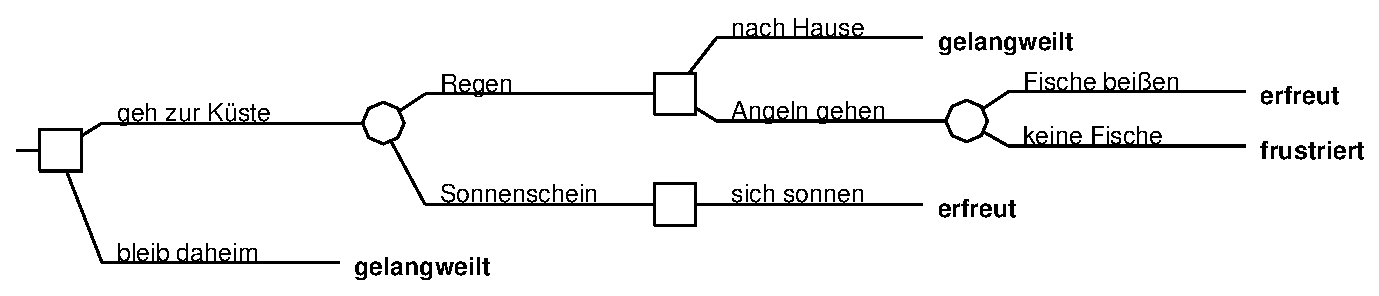
\includegraphics[width=12cm]{Grafiken/Beispiel1_2.eps}
\end{center} 

Erkläutern Sie Ihre
Antwort sowohl anhand der Baum- als auch anhand der Tabellendarstellung (Seite
\pageref{AngelnBeispiel}). Welche Darstellungsform eignet sich dafür besser?

\item Welche Handlungen sollten bei den beiden folgenden Entscheidungs-Tabellen
nach der lexikalischen Maximin-Regel gewählt werden:

\begin{center}
\begin{tabular}{c|c|c|c|c|cc|c|c|c|c|}
\multicolumn{1}{c}{} & \multicolumn{4}{c}{Tabelle 1:} &
\multicolumn{2}{c}{} & \multicolumn{4}{c}{Tabelle 2:}
\\
\cline{2-5} \cline{8-11}
$A_1$ & 1 & -3 & 5   & 6 & & $A_1$ & 0 & 1 & 1 & 3 \\ 
\cline{2-5} \cline{8-11} 
$A_2$ & 2 &  2 & 3   & 3 & & $A_2$ & 0 & 4 & 2 & 3 \\ 
\cline{2-5} \cline{8-11}
$A_3$ & 4 &  6 & -10 & 6 & & $A_3$ & 3 & 0 & 0 & 1 \\ 
\cline{2-5} \cline{8-11}
\end{tabular}

{\tiny Quelle: Michael D. Resnik: Choices. An Introduction to Decision Theory,
Minnesota 2000, S. 27.}
\end{center}

\item Zeige anhand der folgenden Tabelle: Wenn man die lexikalische
Maximin-Regel so abändert, dass der kleinste Wert, sofern er in einer
Zeile mehrmals vorkommt, nicht nur einmal sondern an allen Stellen gestrichen
werden soll, so führt dies dazu, dass durch die lexikalische Maximin-Regel das
Prinzip der Dominanz verletzt werden könnte:

\begin{center}
\begin{tabular}{l|c|c|c|}
\multicolumn{1}{c}{ } & \multicolumn{1}{c}{$S_1$} &
\multicolumn{1}{c}{$S_2$} & \multicolumn{1}{c}{$S_3$}
\\ \cline{2-4}
$A_1$   &    -1  &   2 &  100  \\ \cline{2-4}
$A_2$   &    -1  &  -1 &   3   \\ \cline{2-4}
\end{tabular}
\end{center} 

\item Wie kann man die Maximin-Regel bei Entscheidungsbäumen anwenden?

\item Sei u(x) eine Nutzenskala, die eine Präferenzordnung wiedergibt. Dann gilt:
a) $u(x) > u(y) \Leftrightarrow x \succ y$ und b) $u(x) = u(y) \Leftrightarrow x
\sim y$. {\em Beweise}: Beide Bedingungen gelten auch für die transformierte
Nutzenskala t(u(x)), sofern t der Bedinung für {\em ordinale Transformationen}
genügt: $t(a) > t(b) \Leftrightarrow a > b$ und $t(a) = t(b) \Leftrightarrow a =
b $ für alle a,b auf der Nutzenskala u. 

  ~\\{\bf Schwierigere Aufgabe}\\

\item In der Vorlesung wurde die Präferenzrelation genaugenommen durch zwei
Relationen, nämlich durch die Relation der strikten Präferenz $\succ$ und die
Relation der Indifferenz $\sim$ eingeführt. Zeigen Sie, dass man auch mit einer
einzigen Relation, der schwachen Präferenz $\succeq$ auskommen kann. Geben Sie
dazu geeignete Axiome für die Relation $\succeq$ an. Definieren Sie dann die
Relationen $\succ$ und $\sim$ durch die Relation $\succeq$, und zeigen Sie
anschließend, dass für die so definierten Relationen $\succ$ und $\sim$ die
für sie in der Vorlesung angegeben Axiome gelten.

% \item Für die Olympiade wird eine neue Kombinationssportart aus 5.000m Lauf und
% Weitsprung vorgeschlagen. Für die Beurteilung der Leistungen der Sportler soll
% eine Punktewertung gefunden werden, die so beschaffen ist, dass ein Sportler, der
% im 500m Lauf schneller ist als ein anderer immer auch mehr Punkte bekommt, und
% nur wenn beide Sportler genau gleich gut sind, bekommt derjenige mehr Punkte, der
% im Weitsprung besser abschneidet. Angenommen, die Laufzeiten und die Sprungweiten
% ließen sich unendlich genau messen (m.a.W. es soll angenommen werden, dass die
% Werte reelle Zahlen sind). {\em a) Zeige: Es ist unmöglich eine Punkteskala
% aufzustellen, die beiden Bedingungen genügt.} (Die Moral von dieser Geschichte:
% Nicht alle Arten von wohlgeordneten Präferenzen kann man auf eine lineare
% Nutzenskala abbilden.) {\em b) Zeige weiterhin: Wenn die Messgenauigkeit endlich
% ist, dann ist es sehr wohl möglich eine entsprechende Punkteskala festzulegen.}

% \item Ein Gremium von 5 Personen wird zufällig aus einer Gruppe von 5 Männern und
% 10 Frauen besetzt. Wie groß ist die Wahrscheinlichkeit, dass das Gremium aus 2
% Männern und 3 Frauen besteht? Wie groß ist die Wahrscheinlichkeit, dass das
% Gremium nur aus Frauen besteht?

\end{enumerate}

% \subsection{Zusatzaufgaben}
% 
% \begin{enumerate}
% \item Zeige: Wenn man eine Entscheidungstabelle positiv linear in eine andere
% überführt, dann ist auch die zugehörige Bedauernstabelle eine positiv linear
% transformierte (genaugenommen sogar ein positives Vielfaches, warum?) der
% ursprünglichen Bedauernstabelle. (Was müsste man von der Minimax-Bedauernsregel
% halten, wenn das nicht der Fall wäre?)
% 
% \item Zeige: Positiv lineare Transformationen sind transitiv, d.h. wenn die
% Skala u' durch positiv lineare Transformation aus der Skala u hervorgeht und
% Skala u' durch eine (nicht notwendigerweise dieselbe) positiv lineare
% Transformation in u'' überführt werden kann, dann kann gibt es auch eine
% positiv lineare Transformation, die u unmittelbar in u'' überführt. Warum ist
% diese Eigenschaft wichtig?
% 
% \item Zeige: Jede Entscheidungstabelle kann durch eine positiv lineare
% Transformation in eine Entscheidungstabelle überführt werden, deren maximaler
% Eintrag 1 und deren minimaler Eintrag 0 ist.
% \end{enumerate}

\newpage


\newpage
\section{Entscheidungen unter Unwissenheit II}

In dieser Woche werden wir den Begriff des kardinalen Nutzen (bzw. des
"`Neumann-Morgensternschen"' Nutzens) einführen und einige weitere
Entscheidungsregeln kennen lernen, die auf diesem Nutzenkonzept beruhen. Aus
didaktischen Gründen wird erst ein Beispiel besprochen, in dem bereits der
kardinale Nutzen\footnote{Genaugenommen handelt es sich bei dem folgenden
Beispiel um einen kardinalen Wert, nämlich der Geldwert} vorausgesetzt wird und
erst danach der kardinale Nutzenbegriff selbst eingeführt.

\subsection{Die Minimax-Bedauerns-Regel}
\label{MinimaxRegret}

Von den bisher besprochenen Entscheidungsregeln ist die Maximin-Regel
wahrscheinlich die einleuchtendste und sinnvollste, aber wir haben auch schon
ein Beispiel kennen gelernt, bei dem ihre Anwendung möglicherweise nicht
sinnvoll wäre, und man kann weitere Beispiele konstruieren, bei denen das noch
deutlicher der Fall ist, z.B. das folgende:

\begin{center}
\label{MinimaxBedauernsRegel}
\begin{tabular}{c|c|c|}
\multicolumn{1}{c}{} & \multicolumn{1}{c}{$S_1$} & \multicolumn{1}{c}{$S_2$} \\
\cline{2-3}
$A_1$ & € 1,25 & € 1,50 \\ \cline{2-3}
$A_2$ & € 1,00 & € 50.000 \\ \cline{2-3}
\end{tabular}
\end{center}

Nach der Maximin-Regel müsste die Entscheidung zugunsten der Handlung $A_1$
ausfallen. Aber ist es sinnvoll, sich die Chance auf € 50.000 entgehen zu lassen,
nur um einen möglichen Verlust von 25 Cent zu vermeiden? Wenn man nicht gerade
eine Geschichte erfindet, bei der von diesen 25 Cent Leben und Tod abhängen,
erscheint das mehr als zweifelhaft.\marginline{Minimax-Bedauerns-Regel}  Um
Situationen wie dieser gerecht zu werden, gibt es eine Regel, die darauf zielt,
"`verpasste Chancen"' zu vermeiden. Diese Regel ist die {\em
Minimax-Bedauerns-Regel} (wohlbemerkt: diesmal heißt es "`Minimax"' nicht
"`Maximin"'!). Bei dieser Regel leitet man von der ursprünglichen Tabelle
zunächst eine Bedauernstabelle ab, die für jede Entscheidung und jedes
möglicherweise eintretende Ereignis (bzw. jeden möglichen Weltzustand) die Größe
der verpassten Chance beziffert. Dann wählt man diejenige Entscheidung aus, bei
der die größtmögliche verpasste Chance am kleinsten ist. Die Einträge in der
Bedauernstabelle erhält man, indem man jeden Wert in der Tabelle vom Maximalwert
derselben Spalte abzieht. Für das Beispiel von eben würde die Bedauernstabelle
dann so aussehen:

\begin{center}
\begin{tabular}{c|c|c|}
\multicolumn{1}{c}{} & \multicolumn{1}{c}{$S_1$} & \multicolumn{1}{c}{$S_2$} \\
\cline{2-3}
$A_1$ & € 0    & € 49.998,50 \\ \cline{2-3}
$A_2$ & € 0,25 & € 0 \\ \cline{2-3}
\end{tabular}
\end{center}

Das maximale Bedauern für die Handlung $A_1$ würde also mit € 49.998,50 zu
beziffern sein, während bei der Wahl von $A_2$ schlimmstenfalls ein Verlust
von 25 Cent verschmerzt werden müsste. Um das maximale Bedauern zu minimieren,
muss nach der Minimax-Bedauernsregel also die Handlung $A_2$ gewählt werden.

Ähnlich wie die die Maximin-Regel kann man die Minimax-Be\-dauerns\-regel auch
{\em lexikalisch} mehr\-fach hintereinander anwenden, wenn nicht gleich bei der
ersten Anwendung eine eindeutige Entscheidung getroffen werden kann.

An dieser Stelle könnte jedoch ein Einwand erhoben werden: Beim Übergang von der
Entscheidungstabelle zur Bedauernstabelle haben wir bestimmte Einträge in der
Tabelle voneinander subtrahiert. \marginline{Rechnen mit Nutzenwerten?}
Da es sich um Geldbeträge handelte, war das
denkbar unproblematisch, denn jeder wird zugeben, dass man mit Geldbeträgen
rechnen kann, und dass man sinnvollerweise davon sprechen kann dass € 3 dreimal
so viel Wert sind wie € 1. Aber was ist, wenn wir es nicht mit Geldbeträgen,
sondern wie zuvor mit ordinalen Nutzenwerten zu tun? Den vergleichsweise
voraussetzungsarmen Begriff des ordinalen Nutzens haben wir ja gerade deshalb
eingeführt, weil man mit anderen Werten als Geldbeträgen nicht unbedingt
Rechnungen durchführen kann, selbst wenn sich die Größe des Wertes noch
unterscheiden lässt. (Beispiel: Die meisten Menschen würden wohl zustimmen, dass
Bier und Würstchen leckerer sind als Brot und Wasser, aber es wäre Unsinn zu
sagen, sie sind genau dreimal so lecker.) Wenn wir eine Bedauernstabelle mit
ordinalen Nutzenwerten berechnen würden, dann würde sich das Ergebnis, das bei
der Anwendung der Minimax-Bedauerns-Regel herauskäme ändern, wenn wir die
Nutzenwerte durch ordinal transformierte Nutzenwerte ersetzen, was bei einer
robusten Entscheidungsregel nicht vorkommen sollte. Daher müssen wir entweder auf
die Anwendung der Minimax-Bedauerns-Regel verzichten, oder wir dürfen sie nur
dort anwenden, wo wir einen stärkeren Nutzenbegriff vorausetzen dürfen, wie er
z.B. implizit den in den vorhergehenden Beispielen verwendeten Geldwerten zu
Grunde liegt. Der schwächstmögliche stärkere Nutzenbegriff (stärker im Vergleich
zum ordinalen Nutzen), der es uns erlaubt die Minimax-Bedauerns-Regel anzuwenden,
ist der Begriff des kardinalen Nutzens. 

Bevor wir jedoch auf den Begriff des kardinalen Nutzens eingehen, soll aber
noch auf eine besondere Eigenschaft der Minimax-Bedauerns-Regel hingewiesen
werden, die unter Umständen auch als ein Einwand gegen diese Regel begriffen
werden kann: Die Minimax-Bedauerns-Regel verletzt nämlich -- ebenso wie übrigens auf die
Rangordnungsregel aus Kapitel \ref{Rangordnungsregel} -- das Prinzip der {\em
paarweisen Unabhängigkeit} oder auch "`Unabhängigkeit von dritten
Alternativen"'.\footnote{Die dafür häufig auch verwendete Bezeichnung
"`Unabhängigkeit von irrelevanten Alternativen"' ist wegen ihrer Suggestivität
irreführend. Es ist nämlich keineswegs immer so, dass dritte Alternativen
grundsätzlich irrelevant sind.}
\marginline{Un\-ab\-häng\-ig\-keit von dritten Alternativen}
Fügt man den bestehenden Handlungsalternativen eine Handlungsalternative hinzu,
so kann das selbst dann zu einer Änderung der Entscheidung führen, wenn die neu
hinzugefügte Alternative nach der Minimax-Bedauerns-Regel sowieso nicht gewählt
werden würde. Beispiel:

\begin{center}

\setlength{\parskip}{0.5cm}

\begin{tabular}{c|p{1cm}|p{1cm}|p{1cm}|cc|p{1cm}|p{1cm}|p{1cm}|}
\multicolumn{1}{c}{} & \multicolumn{3}{c}{Entscheidungstabelle} &
\multicolumn{2}{c}{} & \multicolumn{3}{c}{"`Bedauerns"'-tabelle}
\\ \cline{2-4} \cline{7-9}
$A_1$ & 0 & 10 & 4    & & $A_1$ & 5 & 0 & 6  \\ 
\cline{2-4} \cline{7-9} 
$A_2$ & 5 &  2 & 10   & & $A_2$ & 0 & 8 & 0  \\ 
\cline{2-4} \cline{7-9}
\end{tabular}

\begin{tabular}{c|p{1cm}|p{1cm}|p{1cm}|cc|p{1cm}|p{1cm}|p{1cm}|}
\cline{2-4} \cline{7-9}
$A_1$ & 0 & 10 & 4  & & $A_1$ & 10 & 0 & 6  \\ 
\cline{2-4} \cline{7-9} 
$A_2$ & 5 &  2 & 10 & & $A_2$ & 5 &  8 & 0  \\ 
\cline{2-4} \cline{7-9}
$A_3$ & 10 &  5 & 1 & & $A_3$ & 0 &  5 & 9 \\ 
\cline{2-4} \cline{7-9}
\end{tabular}

{\tiny Quelle: Michael D. Resnik: Choices. An Introduction to Decision Theory,
Minnesota 2000, S. 31.}
\end{center}

Die Alternative A3 hat nach der Minimax-Be\-dau\-erns-Re\-gel keine Chance
ge\-wählt zu werden. Dennoch übt ihre Präsenz Einfluss darauf aus, welche der beiden
anderen Handlungsalternativen nach der Minimax-Bedauerns-Regel gewählt wird. Ist
die Alternative A3 abwesend, so ist die Handlung A1 nach der
Minimax-Bedauerns-Regel die beste Handlung. Fügt man die Alternative A3 hinzu, so
ist A2 die beste Handlung.

Sollte man die Abhängigkeit von dritten Alternativen als eine Schwäche der
Minimax-Bedauerns-Regel ansehen? Das hängt wiederum sehr davon ab, in welchem
Zusammenhang die Entscheidungsregel angewandt wird. Da das Prinzip besonders in
der Sozialwahltheorie eine große Rolle spielt, dazu einige Beispiele:

\begin{enumerate}
\label{dritteAlternativen}
  \item Resnik erzählt dazu in etwa die folgende Geschichte \cite[S. 40]{resnik:1987}:
\marginline{Beispiele für die mögliche Relevanz von dritten Alternativen}
Stellen Sie sich vor, Sie sitzen in einem Restaurant und überlegen, ob Sie lieber
ein Steak oder ein vegetarisches Gericht bestellen wollen. Eigentlich mögen Sie
lieber Steak, aber da das Restaurant einen etwas heruntergekommenen Eindruck
macht, haben Sie wegen der Fleischzubereitung so ihre Bedenken und tendieren eher
zu einer vegetarischen Speise. Nun erzählt Ihnen die Dame vom Nebentisch, dass
sie gerade ein vorzügliches Schnitzel gegessen hat. Sie selbst -- nehmen wir an
-- mögen zwar kein Schnitzel, aber obwohl diese Alternative für Sie
"`irrelevant"' ist, wissen Sie nun, dass Sie der Fleischzubereitung in diesem
Restaurant vertrauen können, und bestellen doch das Steak.

  \item Frau Schmidt möchte ein Auto kaufen. Sie legt Wert darauf, dass es das
  teuerste und, wenn nicht das teuerste, dann doch wenigstens dass schnellste
  Auto von der ganzen Stadt ist. Also entscheidet sie sich gegen einen Porsche
  und für einen S-Klasse Mercedes, weil der teurer ist. Jetzt efährt sie aber,
  dass ihre Nachbarin Frau Klein sich kürzlich einen Rolls-Royce zugelegt hat. 
  Einen Rolls-Royce kann sich Frau Schmitt aber sowieso nicht leisten. Da sie
  dann aber statt des teuersten wenigstens das schnellste Auto haben will,
  kauft sie sich nun doch nicht den Mercedes, sondern lieber den Porsche.

  Ihre Wahl zwischen Porsche und Mercedes ist also nicht unabhängig von dritten
  Alternativen, auch diese für Frau Schmitt sowieso nicht in Frage kommen, wie in
  diesem Fall der Rolls Royce.
  
  \item {\em Machinas Paradox}:
\label{machinasParadox}
Angenommen, eine Person habe die Wahl zwischen zwei Lotterien:
\begin{enumerate}
  \item Lotterie: 99\% Chance eine Reise nach Venedig zu gewinnen, 1\%
  Chance eine Filmvorführung über Venedig zu gewinnen.
  \item Lotterie: 99\% Chance eine Reise nach Venedig zu gewinnen, 1\%
  Chance zu Hause zu bleiben.
\end{enumerate}
Im Sinne der Theorie müsste die erste Lotterie eindeutig bevorzugt werden, wenn
man annimmt, dass einen Film über Venedig anzuschauen allemal interessanter
ist, als zu Hause zu sitzen. Andererseits ist es durchaus plausibel sich
vorzustellen, dass angesichts der sehr großen Chance eine Reise nach Venedig zu
gewinnen, es doch noch erträglicher ist zu Hause zu bleiben, wenn man
die Chance verpasst, als sich dann auch noch einen herrlichen Film über Venedig
anschauen zu müssen. 

Wenn man diese Argumentation akzeptiert, dann zeigt das Beispiel einmal mehr,
dass die Annahme der Unabhängigkeit von dritten Alternativen, z.B. auf Grund
solcher psychologischen Faktoren wie des Bedauerns, nicht immer zwingend oder
auch nur glaubwürdig ist. Oder gäbe es vielleicht eine Möglichkeit, das Beispiel
durch eine entsprechende Problemspezifikation, z.B. durch Einbeziehen des Bedauernsfaktors
in die Konsequenz der Entscheidung, doch noch mit der Theorie zu vereinbaren?
(Aufgabe \ref{AufgabeDritteAlternative}!)

\item {\em Mögliche Bedeutung der Rangordnung} \cite[S. 81]{mackie:2003}: Wie
bereits erwähnt ist auch die Rangordnungsregel nicht mit dem Prinzip der
paarweisen Unabhängigkeit vereinbar. Hält man Entscheidungsregeln wie die
Minimax-Bedauernsregel oder die Rangordnugnsregel für sinnvoll, so kann man diese
Unvereinbarkeit statt gegen bestimmte Entscheidungsregeln umgekehrt auch gegen
das Prinzip der paarweisen Unabhängigkeit ausspielen. 

Vorgreifend auf die Sozialwahltheorie sei zur Illustration der möglichen Relevanz
der Rangordnung von Präferenzen und damit auch der Relevanz von dritten
Alternativen folgendes Beispiel diskutiert: Angenommen Napoleon habe die
Präferenzen $b \succ a \succ c \succ d \succ e$ und Josephine $a \succ b \succ c
\succ d \succ e$. Es sei weiterhin angenommen, dass Napoleon und Josephine sich
darauf einigen müssten, ob sie gemeinsam $a$ oder $b$ wählen wollen, und dass
Napoleon sich nach langwierigen Diskussionen schließlich durchgestezt habe sie
gemeinasm $b$ wählen.

Nun erhält Josephine eine Nachricht, die dazu führt, dass sie ihre Präferenzen
dergestalt abändert, dass die Alternative $b$ nun für sie an die letzte Stelle
rückt, so dass sie nun die Präferenzen $a \succ c \succ d \succ e \succ b$ hat. 

Josephine teilt dies Napoleon mit, und bittet darum, auf Grund der geänderten
Umstände die gemeinsame Entscheidung noch einmal zu überdenken. Napoleon
antwortet ihr jedoch mit dem Hinweis auf das Prinzip der Unabhängikeit von
"`irrelevanten"' Alternativen, dass dies nicht erforderlich sei, da sich
Josephines Präferenzen bezüglich $a$ und $b$ duch die neu eingetretenen Umstände nicht
geändert hätten, so dass sie die Entscheidung zwischen $a$ und $b$ gar nicht
beeinflussen dürften.

Sofern man Napoleons Antwort als unverschämt empfindet, ist dieses Beispiel ein
Gegenbeispiel gegen die generelle Gültigkeit des "`Prinzips des Unabhängigkeit
von dritten Alternativen"'. Das Beispiel zeigt, dass das Prinzip der
Unabhängkeit von dritten Alternativen uns zwingt, von der Information über die
Rangordnung der beiden zur Entscheidung anstehenden Alternativen innerhalb einer
größeren Menge von Alternativen zu abstrahieren. Aber unter Umständen könnte
diese Information wichtig sein, z.B. indem sie die Intensität einer Präferenz
ausdrückt und sofern man der Ansicht ist, dass die Intensität der
individuellen Präferenzen bei der Diskussion über gemeinsame Entscheidungen wie
der von Napoleon und Josephine mitberücksichtigt werden sollte.

Man kann es auch so formulieren: Eine dogmatische Festlegung auf das Prinzip
der Unabhängikeit von dritten Alternativen würde Entscheidungsprobleme wie das
von Napoleon und Josephine aus dem Anwendungsbereich der Entscheidungstheorie
ausschließen.


\end{enumerate}
 
Wie man sieht können dritte Alternativen sehr wohl relevant für die relative
Bewertung der anderen Alternativen sein. Insofern muss die Abhängigkeit von
dritten ("`irrelevanten"') Alternativen nicht unbedingt als eine Schwäche der
Entscheidungsregel aufgefasst werden. Aber es gibt andere Situationen, wo das
durchaus der Fall sein kann, etwa bei Wahlen oder Abstimmungen, deren Ergebnis
unter Umständen dadurch manipuliert werden könnte, dass man weitere, scheinbar
irrelevante Alternativen zur Abstimmung stellt.\footnote{Theoretische Beispiele
findet man in der entsprechenden Fachliteratur unter den Stichworten "`Paradox of
Voting"' und "`Agenda Setting"' in Fülle \cite[S. 112ff.]{mueller:2003}. Die
empirische Relevanz des vermeintlichen Problems zyklischer Mehrheiten wird jedoch
inzwischen sehr stark in Zweifel gezogen \cite[S. 147ff.]{green-shapiro:1994}.
Praktisch spielen die Formen der Abstimmungsmanipulation, die in der Public
Choice Literatur so ausführlich erörtert werden, keine Rolle, während andere, die
womöglich viel wichtiger sind, von den Autoren der Public Choice Literatur nicht
beachtet werden.} Insgesamt kann man sagen, dass das Prinzip der
Unabhängigkeit von dritten Alternativen bzw. der paarweisen Unabhängigkeit nur
dann aufgestellt werden sollte, wenn man zuvor sichergestellt hat, dass für die
Entscheidung zwischen jedem Paar von Alternativen (bzw. für die relative
Bewertung von jedem Paar von Alternativen) die Verfügbarkeit der anderen
Alternativen tatsächlich irrelevant ist. In einer Entscheidungssituation, wo
dies nicht der Fall ist, kann eine Theorie, die dieses Prinzip als Axiom
einführt, nicht ohne Einschränkungen angewendet werden.


\subsection{Kardinaler Nutzen}
\label{KardinalerNutzen}
Der Grundgedanke der "`Minimax-Bedauerns-Regel"' besteht darin, eine Entscheidung
zu finden, bei der der maximal mögliche Verlust (je nach eintretenden
Zufallsereignissen) minimiert wird. Da wir diese Regel auf ein Beispiel mit
Geldwerten angewendet haben, konnten wir die Verluste relativ bedenkenlos als die
Differenz zwischen entgangenem Gewinn und erhaltenem Gewinn bestimmen. Aber wie
sollen wir eine solche Regel wie die "`Minimax-Bedauerns-Regel"' anwenden, wenn
die (möglichen) Ergebnisse eines Entscheidungsproblems keine Geldwerte sind? Die
Ihnen zugeordneten Nutzenwerte spiegeln dann -- nach dem Konzept des {\em
ordinalen Nutzens} -- nur eine Rangordnung zwischen den möglichen Ergebnissen des
Entscheidungsprozesses entsprechend den Präferenzen wieder.\marginline{Grenzen
des ordinalen Nutzens} Das Ergebnis der Anwendung einer Entscheidungsregel sollte
also auch nur von der Rangordnung der Nutzenwerte nicht aber von den -- solange
die Ordnung erhalten bleibt -- willkürlich wählbaren Zahlenwerten abhängen, die
diese Ordnung auf einer Nutzenskala wiedergeben. Betrachten wir als Beispiel
einmal folgende beiden Nutzenskalen, die den Ergebnissen $x, y, z$ jeweils einen
bestimmten Nutzen zuordnen. ({\em x}, {\em y} und {\em z} sollen dabei
irgendwelche möglichen Resultate irgendeines Entscheidungsprozesses sein, z.B.
könnten sie für die Resultate {\em frustriert}, {\em gelangweilt}, {\em erfreut}
aus dem Beispiel auf Seite \pageref{AngelnBeispiel} stehen.)

\begin{center}
\begin{tabular}{cc|c|cccc|c|c}
& x  &  y  &  z  &  &  &  x  &  y  &  z  \\ \cline{2-4} \cline{7-9}
\raisebox{1.5ex}[-1.5ex]{Nutzenskala {\bf u()}} 
& 1  &  2  &  3  &  &  
\raisebox{1.5ex}[-1.5ex]{Nutzenskala {\bf v()}}
&  1  &  4  &  9 
\end{tabular}
\end{center}

Beide Skalen geben offenbar denselben ordinalen Nutzen wieder, da $u(z) > u(y) >
u(x)$ und ebenso $v(z) > v(y) > v(x)$. Betrachtet man allerdings die Differenzen, so
fällt auf, dass $u(z) - u(y) = u(y) - u(x)$, während $v(z) - v(y) > v(y) -
v(x)$. Würden diese Nutzenwerte bei einem Entscheidungsproblem auftauchen, so
könnte es geschehen, dass man bei Anwendung der Minimax-Bedauernsregel je
nachdem, ob man die Nutzenfunktion {\em u} oder die Nutzenfunktion {\em v} zur
Darstellung der Präferenzen heranzieht, zu einer anderen
Entscheidungsempfehlung kommt. Genau das dürfte aber nicht geschehen, da {\em
u} und {\em v} nur unterschiedliche Darstellungen desselben {\em ordinalen}
Nutzens sind. Welche Auswege könnte man sich aus dieser misslichen Situation
denken:

\begin{enumerate}
  \item Angesichts des Beispiels (Seite \pageref{MinimaxBedauernsRegel}), mit
  dem wir die Mini\-max-\-Bedauernsregel eingeführt haben, könnte man auf die
  naheliegende Idee verfallen, dass man diese Regel nur in solchen Fällen
  anwenden kann, in denen die Ergebnisse des Entscheidungsprozesses monetäre
  Auszahlungen sind. Das hätte allerdings zwei Nachteile: 1) Die Anwendbarkeit
  der Regel würde dabei auf eine vergleichsweise kleine Menge von
  Entscheidungsproblemen eingeschränkt. 2) In vielen Situationen, in denen in
  irgendeiner Form monetäre Auszahlungen vorkommen, geben die monetären
  Auszahlungen nicht unmittelbar den damit assoziierten Nutzen wieder.
  Hanldungsleitend und damit entscheidungsrelevant ist jedoch
  der Nutzen und nicht der Geldwert.\marginline{Unterschied von Nutzen und
  Geldwert} Ein Beispiel daür, dass Nutzen und Geldwert sich nicht decken müssen
  ist das folgende: 2.000 Euro sind doppelt so viel Geld wie 1.000 Euro. Aber der
  zusätzliche Nutzen, den man von  2.000 Euro Monatsgehalt 
  gegenüber 1.000 Euro Monatsgehalt gewinnt, ist sicherlich geringer 
  als der zusätzliche Nutzen 
  von 1.000 Euro gegenüber 0 Euro Gehalt.
  
  \item Eine andere denkbare Alternative wäre die Aufstellung einer {\em
  qualitativen Bedauernstabelle}. Dazu müsste man zunächst einmal die
  {\em Differenzergebnisse} bestimmen, worunter man zusammengesetzte Ergebnisse
  aus einem nicht eingetretenen und einem statt dessen eingetretenen
  Ergebnis verstehen kann. (In dem Beispiel des Küstenbesuchers aus der ersten
  Vorlesung (Seite \pageref{AngelnBeispiel}), in dem die möglichen Resultate 
  {\em frustriert}, {\em gelangweilt}, {\em erfreut}
  waren, würden sich daraus die Differenzereignisse {\em frustriert statt
  bloß gelangweilt}, {\em gelangweilt statt erfreut} und {\em frustriert statt
  erfreut} ergeben.) Weiterhin müsste man ein neutrales Differenzereignis
  definieren, welches die Stelle der 0 in der aus Nutzenwerten gewonnen
  Bedauernstabelle einnimmt. Dieses neutrale Differenzergebnis könnte man z.B.
  als "`Unter gegebenen Umständen so gut wie möglich"' bezeichnen oder ähnlich.
  Schließlich müsste man die Präferenzen bezüglich der Differenzergebnisse
  bestimmten, denen man dann eine neue ordinale Nutzenfunktion zuweisen könnte.
  Die Bestimmung des minimalen größten Bedauerns erfolgt wie zuvor beschrieben
  (Siehe Abschnitt \ref{MinimaxRegret}). Der Nachteil dieses Vorgehens besteht
  erstens darin, dass die Präferenzordnung für eine weitere Ergebnismenge,
  nämlich die Menge der Differenzergebnisse, bestimmt werden muss, und zweitens
  darin, dass sich dieses Verfahren tatsächlich nur auf die
  Minimax-Bedauerns-Regel anwenden lässt, nicht mehr aber auf
  die meisten weiteren Entscheidungsregeln,
  die wir gleich noch kennen lernen werden. In den Fällen aber, in denen wir
  nicht die gleich zu besprechende Neuman-Morgensternsche Nutzenfunktion bilden
  können (d.h. in den Fällen, in denen wir aus empirisch-sachlichen
  Gründen höchstens einen {\em ordinalen} Nutzen voraussetzen dürfen) bleibt die
  Bildung einer qualitativen Bedauernstabelle die einzige Alternative.
    
  \item Schließlich kann man versuchen, ein "`stärkeres"' Nutzenkonzept als das
  des ordinalen Nutzens zu Grunde zu legen.\marginline{kardinaler Nutzen}
  Bei einem solchen Nutzenkonzept
  müsste nicht nur die Ordnung der Nutzenwerte unter einer Transformation
  erhalten bleiben sondern mindestens auch die Ordnung beliebiger Differenzen
  von Nutzenwerten. Stärker ist ein solches Nutzenkonzept in dem Sinne,
  dass die Nutzenwerte dann mehr Informationen enthalten als nur die
  Information über die Ordnung der Präferenzen. Das bedeutet aber auch, dass
  ein solches Nutzenkonzept empirisch schwerer zu rechtfertigen ist, und dass
  der empirische Anwendungsbereich eines solches Nutzenkonzepts
  kleiner sein wird als der des ordinalen Nutzens. Um
  die Ordnung der Differenzen zu erhalten, ist es aber andererseits noch längst
  nicht erforderlich, den konkreten Zahlenwerten der Nutzenfunktion eine
  eindeutige Interpretation zu geben, wie dies bei der Zuweisung von Geldwerten
  der Fall wäre. Gesucht ist also ein möglichst schwaches (und damit 
  empirisch immer noch möglichst breit anwendbares) Nutzenkonzept, das
  aber stärker ist als das des Ordinalen Nutzens. 
  Ein solches Nutzenkonzept ist das des {\em
  kardinalen} bzw. des {\em Neumann-Morgensternschen Nutzens}.
\end{enumerate}

Das, was wir eben eher intuitiv die "`Stärke"' eines Nutzenkonzepts genannt
haben, ist dadurch bestimmt, unter welcher Art von Transformationen man zwei
Nutzenfunktionen als {\em äquivalent}, d.h. denselben Nutzen ausdrückend,
betrachtet. (Man kann es also nicht den Nutzenfunktionen also solchen ansehen, ob
sie einen ordinalen oder kardinalen Nutzen ausdrücken. Sondern erst durch den
Vergleich von Nutzenfunktionen und der Festlegung der Bedingungen ihrer
Äquivalenz oder Nicht-Äquivalenz wird dies bestimmt.) Beim {\em ordinalen Nutzen}
wurden alle Nutzenfunktionen als äquivalent betrachtet, die durch
"`ordnungserhaltende"' Transformationen ineinander überführt werden können.
"`Ordnungserhaltend"' sind alle streng monoton steigenden Abbildungen. Der {\em
kardinale Nutzen} ist nun dadurch definiert, dass zwei Nutzenfunktionen als
äquivalent betrachtet werden, wenn man sie durch {\em positive lineare
Transformationen} ineinander überführen kann. Positive lineare Transformationen
sind alle Transformationen der Form:

\begin{displaymath}
u(x) = ax + b, \qquad a > 0
\end{displaymath}

Man betrachte unter diesem Gesichtspunkt einmal die folgenden, in
Tabellen dargestellten Nutzenfunktionen:

\begin{center}
\begin{tabular}{cc|c|cccc|c|cccc|c|c|}
& x  &  y  &  z  &  &  &  x  &  y  &  z & & & x & y & z \\ 
\cline{2-4} \cline{7-9} \cline{12-14}
\raisebox{1.5ex}[-1.5ex]{{\bf u()}} 
&  1  &  2  &  3  &  &  
\raisebox{1.5ex}[-1.5ex]{{\bf v()}}
&  1  &  4  &  9 &  &
\raisebox{1.5ex}[-1.5ex]{{\bf w()}}
&  1  &  3  &  5
\end{tabular}
\end{center}

Alle drei Nutzenfunktionen geben denselben ordinalen Nutzen wieder, aber nur die
Funktionen {\em u} und {\em w} geben denselben kardinalen Nutzen wieder, da $w(x)
= 2u(x)-1$. Weiterhin kann man sich leicht überlegen, dass zwei Nutzenfunktionen,
die denselben kardinalen Nutzen darstellen, immer auch denselben ordinalen Nutzen
repräsentieren, denn positive lineare Transformationen sind immer auch
ordnungserhaltende Transformationen. Umgekehrt gilt dasselbe aber nicht, wie die
Tabelle oben zeigt. Kardinale Nutzenskalen sind "`feinkörniger"' als ordinale
Nutzenskalen.
\marginline{Erhalt der Ordnung von Nutzendifferenzen}
Und sie erhalten, wie erwünscht nicht nur die Ordnung der Nutzenwerte sondern
auch die Ordnung der Differenzen von Nutzenwerten, denn seien $x,y,z,w \in
\mathbb{R}$ beliebige Nutzenwerte und sei $u(x) = ax + b$ mit $a,b \in
\mathbb{R}, a > 0$ eine positive lineare Transformation, dann:
\begin{eqnarray*}
  x - y & > & z - w  \\
  a(x-y) & > & a(z-w)  \\
  a(x-y) + b - b & > & a(z-w) + b - b \\
  (ax + b) - (ay + b) & > & (az + b) - (aw + b) \\
  u(x) - u(y) & > & u(z) - u(w) 
\end{eqnarray*}
Dasselbe gilt, wenn man statt des Ungleichheitszeichens ein Gleichheitszeichen
einsetzt, womit der Erhalt der Ordnung von Nutzendifferenzen unter positiv
linearer Transformation bewiesen ist. Positive lineare Transformationen haben 
darüber hinaus die Eigenschaft, dass sie nicht bloß die
Ordnung der Differenzen von Nutzenwerten erhalten, sondern auch die Quotienten
der Differenzen:\marginline{Erhalt der Quotienten von Nutzendifferenzen}
\[ \frac{u(x) - u(y)}{u(z) - u(w)} = 
   \frac{(ax + b) - (ay + b)}{(az + b) - (aw + b)} = 
   \frac{a(x - y) + b-b}{a(z - w) + b-b} = 
   \frac{x - y}{z - w} \]
Diese Eigenschaft wird später noch für uns wichtig werden wird. Erfüllt eine
Skala, wie in diesem Fall die kardinale Nutzenskala, diese Eigenschaft, so nennt
man sie auch eine {\em Intervallskala}. Zur besseren Übersicht sollen im
folgenden kurz einige der wichtigsten Skalentypen aufgelistet werden, die in
der Wissenschaft von Bedeutung sind.

\subsubsection{Exkurs: Skalentypen}

Skalen dienen dazu abgestufte Größen darzustellen. Nun gibt es unterschiedliche
Grade, in denen irgendwelche Größen abgestuft sein können. (Mit dem ordinalen
und dem kardinalen Nutzen haben wir schon zwei unterschiedliche Abstufungsgrade
kennen gelernt.) Diese unterschiedlichen Abstufungsgrade spiegeln sich in
den verschiedenen Skalentypen wieder. Die Skalentypen sind dabei von gröberen zu
immer feineren Skalentypen geordnet. (Vgl. zum folgenden \cite[S.
73ff.]{schurz:2006}) 

Das gröbste bzw. "`niedrigste"' Skalenniveau, das man sich vorstellen kann, ist
das einer {\bf Nominalskala}\marginline{Nominalskala}. Bei einer Nominalskala
wird die gegebene Größe lediglich in eine von mehreren begrifflichen Kategorien 
eingordnet, ohne dass
zwischen diesen Kategorien eine Ordnung des Mehr- und Weniger besteht. Man
spricht deshalb auch von "`Kategorienskalen"' oder von
"`qualitativ-klassifikatorischen Begriffen"'. Ein Beispiel wäre etwa die
Zuordnung von Wirtschaftsunternehmen zu unterschiedlichen Wirtschaftssektoren wie
a) Landwirtschaft, b) Handel und Industrie, c) Dienstleistung. Die einzigen
Bedinungen, denen eine Nominalskala genügen muss, bestehen darin, dass die
Kategorien 1. {\em disjunkt} (kein Gegenstand kann unter mehr als eine Kategorie
gleichzeitig fallen) und 2. {\em exhaustativ} (jeder Gegenstand kann in
mindestens eine Kategorie eingeordnet werden) sein müssen. Eine wie auch immer
geartete Ordnungsbeziehung muss zwischen den Kategorien aber nicht bestehen. (Man
kann ja auch z.B. kaum sinnvollerweise sagen, dass Dienstleistung "`mehr"' oder
"`größer"' ist als Landwirtschaft. Allenfalls könnte man das von der Anzahl der
Beschäftigten oder dem erwirtschafteten Umsatz in dem entsprechenden Sektor
sagen.)

Das nächsthöhere Skalenniveau stellt die {\bf
Ordinalskala}\marginline{Ordinalskala/ Rangskala} (auch "`Rangskala"') dar. Im
Gegensatz zur Nominalskala werden hier die Merkmale bzw. die Objekte des
Gegenstandsbereichs in "`Ranggruppen"' eingeteilt, zwischen denen eine Höher- und
Niedriger-Beziehung besteht. (Für die präzise Definition einer solchen {\em
Quasi-Ordnungs}-Beziehung siehe Seite \pageref{Ordnungsaxiome}) Außer dem nun
schon bekannten ordinalen Nutzen, wäre ein weiteres Beispiel die Mohs-Skala aus
der Mineralogie, bei der die Härte von Mineralien danach geordnet wird, welches
Mineral welche anderen "`ritzt"' \cite[S. 75]{schurz:2006}.

Auf die Ordinalskala folgt in der Rangfolge die {\bf
Intervallskala}\marginline{Intervallskala}. Intervallskalen verfügen über eine
mehr oder weniger willkürlich gewählte Maßeinheit. Weder die Maßeinheit selbst
noch der Nullpunkt einer Intervallskala sind in irgendeiner Weise durch den
Gegenstandsbereich festgelegt. Voraussetzung ist jedoch, dass die auf einer
Intervallskala abgebildete Größe zahlenmäßig empirisch messbar ist. Die
Maßeinheit erlaubt es dann, Differenzen und Quotienten von Differenzen der
gemessenen Größe zu vergleichen. Beispiele sind denn auch Orts- und
Zeitmessungen, denn ob man das Jahr 0 auf Christi Geburt oder auf den Zeitpunkt
der Auswanderung Mohammeds nach Medina verlegt, ist eine Sache bloßer Konvention,
genauso wie es eine Konvention ist, dass der Nullmeridian in Greenwich liegt.
Trotzdem kann man Zeit- und Ortsdifferenzen sowie Quotienten von Differenzen
vergleichen (eine Stunde ist solange wie jede andere und drei Stunden sind
dreimal solange wie eine Stunde).

Die {\bf Verhältnisskala}\marginline{Verhältnisskala} schießlich unterscheidet
sich von der Intervallskala dadurch, dass nur noch die Maßeinheit willkürlich
festgelegt ist, der Nullpunkt aber durch die Wirklichkeit vorgegeben ist.
Beispiele dafür sind etwa Gewichtsskalen oder auch die Temperaturskala nach
Kelvin, die den Nullpunkt auf den "`absoluten Nullpunkt"' bei 273,15 Grad Celsius
verlegt. Auch Geldwerten liegt eine Verhältnisskala zu Grunde, denn der Nullpunkt
(d.h. wenn jemand gar kein Geld hat) ist ja in naheliegender Weise vorgegeben.

Schließlich kann man von allen vorhergehenden Skalen noch die {\bf
Absolutskala}\marginline{Absolutskala} unterscheiden, bei der man verlangen
müsste, dass auch die Maßeinheit selbst noch eine zwingende empirische
Interpretation hat. Dergleichen ist aber im Grunde nur bei einfachen Zählskalen
der Fall. Wenn man also z.B. von "`drei Äpfeln"' spricht, dann hat die Zahl drei
dabei einen ganz bestimmten empirischen Sinn und es ist nicht eine Frage der
Konvention ob man drei oder zwei sagt, wie es eine Frage der Konvention ist, ob
man eine Länge in Meter oder Fuß angibt.

Insgesamt ergibt sich also eine Abfolge von fünf Skalentypen: 

\begin{center}
{\small Nominalskala < Ordinalskala < Intervallskala < Verhältnisskala <
Absolutskala}
\end{center}

Im Anschluss an diese Auflistung von Skalentypen stellen sich zwei naheliegende
Fragen: Erstens: Sind das alle Skalentypen, die es gibt? Und zweitens: Wonach
richtet sich, welchen Skalentyp man verwenden kann oder soll?

Was die erste Frage betrifft, so sind die aufgeführten Skalentypen natürlich
längst nicht alle denkbaren Skalentypen. Einmal könnte man die Abfolge von
Skalentypen sehr wohl noch weiter verfeinern.\marginline{Mehr\-dim\-en\-sion\-ale
Skalen} Dann gibt es, was noch wichtiger ist, neben den hier aufgeführten
eindimensionalen Skalen auch mehrdimensionale Skalen. Zu diesen zählen
beispielsweise Farbskalen bzw. Farbräume. Im RGB-Farbraum etwa wird jede Farbe
durch ein 3-tupel des Rot-, Grün- und Blauwertes angegeben, aus denen die Farbe
nach dem Prinzip der additiven Mischung zusammengesetzt ist.

Was die zweite Frage betrifft,\marginline{Auswahl des Skalentyps} so richtet sich
die Verwendung eines bestimmten Skalentyps nach den {\em empirischen
Eigenschaften} der auf der Skala abgebildeten Größe und nach den {\em vorhandenen
Messmethoden}. So kann man die Länge deshalb auf einer Intervallskala messen,
weil wir mit dem "`Urmeter"' über einen entsprechenden Vergleichsmaßstab
verfügen. Bei der Härtemessung von Materialen nach der Mohs-Skala gibt es keinen
solchen Vergleichsmaßstab, so dass sie auch nicht auf einer Intervallskala,
sondern nur auf einer Ordinalskala angegeben werden kann.

Besonders schwierig gestaltet sich die Suche nach geeigneten Messmethoden und
damit die "`Metrisierung"'\marginline{Schwierigkeiten der Metrisierung in den
Sozialwissenschaften} (d.h. die Überführung von komparativen Begriffe in
quantitative mittels geeigneter Messmethoden) in den Sozialwissenschaften. Denn
während die verschiedenen Zahlenmengen von den natürlichen Zahlen bis hin zu den
komplexen Zahlen geradezu dafür geschaffen scheinen, die Zusammenhänge
auszudrücken, die die Naturwissenschaften untersuchen (dazu sehr eindrucksvoll
Penrose \cite[S. 51ff.]{penrose:2004}), weshalb man in diesem Bereich recht
eigentlich sagen darf, dass die Mathematik die Sprache der Natur ist, lassen sich
mathematische Gesetze für die Sozialwissenschaften vielfach nur unter erheblicher
Strapazierung der Begriffe einspannen. Diese Schwierigkeiten begegnen uns auch
beim Präferenzbegriff, denn während man die Annahme, dass es ordinale Präferenzen
(soll heißen: Präferenzen, die durch ordinale Nutzenfunktionen beschrieben
werden können) gibt, noch einigermaßen glaubwürdig rechtfertigen kann, und es zumindest
vorstellbar erscheint, die Ordnung von Präferenzen durch Befragung oder
Verhaltensbeobachtung halbwegs zuverlässig festzustellen, so ist dies bei der
Annahme kardinaler Präferenzen nur unter Schwierigkeiten möglich. Wenn man aber
annimmt, dass bei solchen Gegenständen, deren Wert sich durch Geld ausdrücken
lässt (also bei "`Waren"') der kardinale Nutzen einigermaßen mit dem Geldwert
korreliert, dann erscheint die Annahme nicht ganz abwegig, dass es so etwas wie
kardinale Präferenzen geben könnte.

Eine weitere Schwierigkeit, die mit der Beantwortung der Frage, welche Art von
Skala man zur Nutzenmessung verwenden darf, noch gar nicht berührt ist, ist die
ob Nutzenbewertungen immer nur jeweils für eine Person gültig sind, 
\marginline{Problem intersubjektiver Nutzenvergleiche} oder ob man
auch die Nutzenwerte unterschiedlicher Personen untereinander vergleichen darf
({\em intersubjektiver Nutzen}). In Bezug
auf solche Güter, deren Wert von den meisten Menschen gleich hoch geachtet wird
(z.B. Gesundheit, Leben, Wohlstand, Jugend etc.) erscheint ein intersubjektiver
Nutzenvergleich nicht abwegig. Ebenso erscheint ein intersubjektiver
Nutzenvergleich bei Gütern möglich, für die soziale Institutionen existieren, die
solche Nutzenvergleiche hervorbringen, wie das z.B. Märkte für Waren tun. Bei
anderen Gütern mag das nicht immer möglich sein. Mit den beiden Unterscheidungen
kardinaler Nutzen - ordinaler Nutzen und subjektiver Nutzen - intersubjektiver
Nutzen ergeben sich insgesamt vier Arten von Nutzenkonzepten:
\begin{center}
\begin{tabular}{cc|p{3.2cm}|p{3.2cm}|}
& \multicolumn{1}{c}{} & \multicolumn{2}{c}{Skalentyp} \\
&                  & \multicolumn{1}{c|}{\em ordinal}
                   & \multicolumn{1}{c}{\em kardinal}
\\ \cline{2-4}
& \raisebox{-1.5ex}[1.5ex]{\em subjektiv}  & subjektiver \mbox{ordinaler
Nutzen} & subjektiver \mbox{kardinaler Nuzen}   \\
\cline{2-4}
\raisebox{1.5ex}[-1.5ex]{Vergleichbarkeit}
& \raisebox{-1.5ex}[1.5ex]{\em intersubjektiv}
& intersubjektiver \mbox{ordinaler Nutzen} &
intersubjektiver \mbox{kardinaler Nutzen} \\
\cline{2-4}
\\
\end{tabular}
\end{center}
Spiel- und entscheidungstheoretische Modelle kann man danach einteilen, welche
Art von Nutzen sie voraussetzen. Die empirische Anwendbarkeit solcher Modelle
hängt dann immer davon ab, ob man in einer gegebenen Anwendungssituation das
vorausgesetzte Nutzenkonzept rechtfertigen kann oder nicht (was in der Regel
wiederum eine Frage des Vorhandenseins zuverlässiger Bestimmungsmethoden der
Nutzenwerte des vorausgesetzten Nutzenkonzepts in der gegebenen Anwendungssituation 
ist).

\subsection{Weitere Entscheidungsregeln auf Basis des kardinalen Nutzens}
\subsubsection{Die Optimismus-Pessimismus Regel}

Für die Theorie- und Modellbildung ist der kardinale Nutzen deshalb so
vorteilhaft, weil er es erlaubt, in einem gewissen Rahmen mit Nutzenwerten zu
rechnen. Mit Hilfe des kardinalen Nutzenbegriffs können wir daher nicht nur
endlich guten Gewissens die Minimax-Bedauerns-Regel anwenden, sondern gleich
auch eine ganze Reihe weiterer Entscheidungsregeln erfinden. Eine davon ist die
"`Optimismus-Pessimismus"'-Regel. Diese Regel funktioniert folgendermaßen:
Zunächst legen wir einen Optimismusindex $a$ fest, der zwischen 0 und 1
liegen muss. Dann wählen für jede Handlung (also aus jeder {\em Zeile} der
Entscheidungstabelle) das beste und das schlechteste mögliche Ergebnis
aus. Das beste Ergebnis können wir der Einfachheit halber mit $MAX$
bezeichnen, das schlechteste nennen wir $min$. Nun berechnen wir für jede
Handlung eine Bewertung $R_a$ ("`R"' wie "`rating"') nach folgender Formel:
\marginline{Bewertung mit Hilfe des Optimismusindex}
\begin{displaymath}
R_a = aMAX + (1-a)min
\end{displaymath}
Schließlich wählen wir diejenige Handlung aus, für die $R_a$ am größten ist.
Welche Handlung gewählt wird hängt dabei ganz wesentlich von der Wahl des
Optimismusindex $a$ ab. Aber das ist auch gewollt, denn bei dieser
Entscheidungsregel geht es darum zuerst festzulegen, wie "`optimistisch"' man
sein möchte, und dann auf dieser Grundlage die eigentliche Entscheidung zu
treffen. Die beiden Grenzfälle $a=0$ und $a=1$ entsprechen übrigens
haargenau der letzte Woche besprochenen Maximin ($a=0$) und Maximax-Regel
($a=1$). Die Anwendung der Regel kann an folgendem Beispiel verdeutlicht werden:
\begin{center}
\begin{tabular}{c|c|c|c|}
\multicolumn{1}{c}{}  & \multicolumn{1}{c}{S1}  & \multicolumn{1}{c}{S2}  & 
\multicolumn{1}{c}{S3} 
\\ \cline{2-4}
 A1 & 9 & 1 & 2 \\ \cline{2-4}
 A2 & 5 & 6 & 3 \\ \cline{2-4}
\end{tabular}
\end{center}
Für a = 0.5 ergibt sich:
\begin{eqnarray*}
& R_{A1} = 0.5 \cdot 9 + 0.5 \cdot 1 = 5.0 & \\
& R_{A2} = 0.5 \cdot 6 + 0.5 \cdot 3 = 4.5 & \\
\end{eqnarray*}
Bei einem Optimismus-Index von 0.5 sollte also die Handlung A1 gewählt werden.

Für a = 0.2 ergibt sich dagegen:
\begin{eqnarray*}
& R_{A1} = 0.2 \cdot 9 + 0.8 \cdot 1 = 2.6 & \\
& R_{A2} = 0.2 \cdot 6 + 0.8 \cdot 3 = 3.6 & \\
\end{eqnarray*}
In diesem Fall sollte die Handlung A2 gewählt werden.

Die Handlungsempfehlung, die sich aus der Anwendung
der Optimismus-Pessimismus-Regel ergibt, hängt wie zu erwarten von der Wahl des
Optimismusindex ab. Auch wenn diese Wahl willkürlich ist, stellt sich doch die
Frage, ob es ein Verfahren gibt, um die Wahl wenigstens sinnvoll zu treffen,
oder anders formuliert: Woher weiss ich eigentlich wie optimistisch ich sein
will? Ein Verfahren, das zu Bestimmung des Index vorgeschlagen worden ist, ist
dieses (vgl. \cite[S. 33]{resnik:1987}): 
\marginline{Bestimmung des Optimismusindex} Man nehme die folgende 
einfache Entscheidungstabelle, in welcher in der ersten Zeile die Nutzenwerte 0
und 1 (einer beliebigen kardinalen Nutzenskala) und in der zweiten Zeile in beiden
Spalten ein unbekanntes Ergebnis {\em x} eingetragen worden ist:
\begin{center}
\begin{tabular}{c|c|c|}
\multicolumn{1}{c}{}  & \multicolumn{1}{c}{S1}  & \multicolumn{1}{c}{S2} 
\\ \cline{2-3}
 A1 & 0 & 1 \\ \cline{2-3}
 A2 & x & x \\ \cline{2-3}
\end{tabular}
\end{center}
Dabei soll diesmal die Frage nicht lauten, welche Handlung gewählt werden soll
(um ein möglichst gutes Ergebnis zu erzielen), sondern es soll vielmehr schon
vorgegeben sein, dass wir zwischen den Handlungen A1 und A2 indifferent sind.
Nun müssen wir x genau so groß wählen, dass wir zwischen A1 und A2 tatsächlich
indifferent sind. Haben wir x entsprechend gewählt, dann können wir daraus den
Optimismus-Pessimismusindex ableiten, denn auf Grund der Indifferenz gilt:
\begin{eqnarray*}
R_{A1} & = & R_{A2} \\
a \cdot 1 + (1-a) \cdot 0 & = & a \cdot x + (1-a) \cdot x \\
a & = & x
\end{eqnarray*}
Was ist damit gewonnen? Wir haben auf diese Weise die Wahl des Optimismusindex
aus der Wahl (bzw. Entscheidung im {\em dezisionistischen} Sinne) über die
Indifferenz zwischen zwei Handlungsalternativen abgeleitet. Wenn man annimmt,
dass es leichter ist, anzugeben, ob man zwischen zwei Alternativen indifferent
ist, als die Frage zu beantworten, wie hoch man den eigenen Optimismus auf
einer Skala zwischen 0 und 1 einschätzt, dann vereinfacht das die Wahl des
Optimusmusindex. Wir hätten dann eine Willkürentscheidung auf eine andere
zurückgeführt, die zu treffen uns möglicherweise leichter fällt.

\marginline{Einwände:}
Allerdings wirkt dieses Verfahren etwas gezwungen. Vor allem gibt es einen
gravierenden Einwand:\marginline{1.Risiko\-be\-reit\-schaft ist
situationsspezifisch} Die Frage wie optimistisch oder pessimistisch man
entscheiden sollte, oder, was auf dasselbe hinausläuft, wie risikofreudig oder
risikoavers man sich verhält, dürfte von den meisten Menschen hochgradig
situationsspezifisch beantwortet werden. Insofern erscheint es äußerst
fragwürdig, einen Optimismusindex, den man durch ein abstraktes
Gedankenexperiment bestimmt hat, auf irgendeine konkrete Entscheidungssituation
zu übertragen, der man möglicherweise ein ganz anderes Risikoverhalten zu Grunde
legen möchte. Dann kann man sich das Gedankenexperiment besser gleich sparen und
willkürlich bleibt die Entscheidung über den Optimismusindex ohnehin.

Dieses Willkürelement ist noch aus einem anderen Grund als dem der Schwierigkeit
der Festlegung des Optimismusindex problematisch:
\marginline{2.Nachträgliche "`Rationalisierung"' von Entscheidungen}
Wenn eine Entscheidungsregel derartige Willkürelemente enthält, dann lädt sie
geradezu dazu ein, zuerst die Entscheidung vollkommen intuitiv zu treffen, und
sie erst im Nachhinein durch die Wahl eines geeigneten Index zu
"`rationalisieren"'. Das könnte besonders dann problematisch werden, wenn die
entscheidungtreffenden Personen anderen für ihre Entscheidung
rechenschaftspflichtig sind, denn es lässt sich dann nicht mehr nachvollziehen,
ob die Entscheidung tatsächlich "`verantwortlich"' getroffen wurde.

Daneben ist die Optimismus-Pessimismus-Regel mit ähnlichen Schwierigkeiten
behaftet, wie die Maximin und die Minimax-Bedauerns-Regel. 
\marginline{3.Ver\-nach\-läs\-si\-gung mittlerer Optionen}
Da sie jeweils nur
zwei Werte jeder Zeile in das Kalkül einbezieht, lassen sich leicht Fälle
konstruieren, in denen sie unplausibel erscheint:
\begin{center}
\begin{tabular}{c|c|c|c|c|c|c|}
\multicolumn{1}{c}{ } & \multicolumn{1}{c}{$S_1$} &
\multicolumn{1}{c}{$S_2$} & \multicolumn{1}{c}{$S_3$} & 
\multicolumn{1}{c}{\ldots} & 
\multicolumn{1}{c}{$S_{99}$} & \multicolumn{1}{c}{$S_{100}$} \\ \cline{2-7}
$A_1$ & 2 & 1 & 1 & $\cdots$ & 1 & 0 \\ \cline{2-7}
$A_2$ & 2 & 0 & 0 & $\cdots$ & 0 & 0 \\ \cline{2-7}
\end{tabular}
\end{center}

In diesem Fall würde die Optimismus-Pessimismus-Regel immer zur Indifferenz
zwischen beiden Handlungen führen, obwohl intuitiv die Handlung A1 sicherlich
als die bessere beurteilt werden müsste. 

Schließlich existiert noch ein weiterer Einwand, der auf einer etwas
raffinierteren Konstruktion beruht, nämlich auf der sogenannten
"`Mischungsbedingung"' ({\em mixture-condition}),
\marginline{Mischungs\-be\-ding\-ung}
 die -- leicht vereinfacht --
besagt: Wenn eine Person indifferent zwischen zwei Handlungsalternativen ist,
dann ist sie auch indifferent zwischen diesen beiden Handlungen und einer dritten
Handlung, die darin besteht, eine Münze zu werfen und bei "`Kopf"' die erste
Handlung und bei "`Zahl"' die zweite Handlung zu wählen. Betrachten wir die
folgende Tabelle:

\begin{center}
\begin{tabular}{c|c|c|}
\multicolumn{1}{c}{}  & \multicolumn{1}{c}{S1}  & \multicolumn{1}{c}{S2} 
\\ \cline{2-3}
 A1 & 0 & 1 \\ \cline{2-3}
 A2 & 1 & 0 \\ \cline{2-3}
\end{tabular}
\end{center}

Nach der Optimismus-Pessimismus-Regel herrscht zwischen beiden
Handlunsalternativen völlige Indifferenz, und zwar unabhängig von der Wahl des
Optimismusindex {\em a}. Fügt man nun die Münzwurfalternative hinzu, dann
ergibt sich folgende Entscheidungstabelle:\footnote{Bei der Nutzenbewertung der
Ergebnisse der Münzwurfhandlung wurde implizit bereits die {\em
Erwartungsnutzenhpyothese} zugrunde gelegt, die besagt, dass der
Erwartungsnutzen gleich dem erwarteten Nutzen multipliziert mit der
Eintrittswahrscheinlichkeit ist. Strenggenommen kann auch das Ergebnis der
Münzwurfhandlung nur 0 oder 1 sein.}

\begin{center}
\begin{tabular}{c|c|c|}
\multicolumn{1}{c}{}  & \multicolumn{1}{c}{S1}  & \multicolumn{1}{c}{S2} 
\\ \cline{2-3}
 A1 & 0 & 1 \\ \cline{2-3}
 A2 & 1 & 0 \\ \cline{2-3}
 A3 & $\frac{1}{2}$ & $\frac{1}{2}$ \\ \cline{2-3}
\end{tabular}
\end{center}

Angenommen der Optimismus-Pessimismus-Index wäre $a = \frac{2}{3}$. Dann ergibt
sich daraus:
\marginline{4.Verletzung der "`Mischungs\-bedingung"'}
\begin{eqnarray*}
R_{A1} & = \frac{1}{3} \cdot 0 + \frac{2}{3} \cdot 1 = & 2/3 \\
R_{A2} & = \frac{2}{3} \cdot 1 + \frac{1}{3} \cdot 0 = & 2/3 \\
R_{A3} & = \frac{2}{3} \cdot \frac{1}{2} + \frac{1}{3} \cdot \frac{1}{2} =
\frac{1}{2}
\end{eqnarray*}
Nach der Optimismus-Pessimismus-Regel müssten die Handlungen A1 und A2 der
"`Münzwurfalternative"' vorgezogen werden, unter Verletzung der
Mischungsbedingung. Die Mischungsbedingung lässt sich nur erfüllen, wenn das
beste und das schlechteste mögliche Ergebnis genau gleich gewichtet
werden, d.h. bei einem Optimismusindex von $a=\frac{1}{2}$. 

\marginline{Einwände gegen die Mischungsbedingung}
Wie auch bei den denkbaren Einwänden gegen die anderen Entscheidungsregeln, lässt
sich darüber streiten, ob die Verletzung der "`Mischungsbedingung"' ein Nachteil
oder, eher im Gegenteil, eine besondere Eigenschaft der
Optimismus-Pessimismus-Regel ist. ("`It's not a bug, it's a feature!"') Wenn
jemand optimistisch ist, dann besagt das ja gerade, dass die Person eher geneigt
ist, an den Erfolg zu glauben als an eine 50:50 Chance von Erfolg und Misserfolg,
so dass es nicht verwunderlich ist, dass sie eine Handlung, an deren Erfolg sie
glaubt, einem Münzwurf vorzieht, von dem sie weiß, dass die Chancen
gleichverteilt sind. Widersprüchlich wäre das optimistische (oder pessimistische)
Verhalten bei der gegebenen Entscheidungstabelle aber immer noch insofern, als
die Person eigentlich nur {\em entweder} an den mehr als 50\%-igen Erfolg von S1
{\em oder} von S2 glauben dürfte, aber -- sofern die Zustände S1 und S2 von den
Handlungen unabhängig sind -- nicht daran, dass sie in jedem Fall die höheren
Erfolgschancen hat.

\subsubsection{Das Prinzip der Indifferenz}
\label{Indifferenzprinzip}
Wenn wir die Nutzenwerte als kardinale Nutzenwerte interpretieren und daher mit
ihnen rechnen dürfen, wie das bei der Optimismus-Pessimismus-Regel der Fall
ist, dann besteht eine der naheliegendsten Arten, die unterschiedlichen
Handlungsalternativen in eine Rangordnung zu überführen, darin, einfach alle
Zahlen in jeder Zeile aufzusummieren und die Handlungsalternative mit der
höchsten Zeilensumme zu wählen. An einem Beispiel betrachtet sieht das
Verfahren folgendermaßen aus:

\begin{center}
\begin{tabular}{c|c|c|c|c|c|cc}
\multicolumn{1}{c}{ } & \multicolumn{1}{c}{$S_1$} &
\multicolumn{1}{c}{$S_2$} & \multicolumn{1}{c}{$S_3$} & 
\multicolumn{1}{c}{$S_4$} & 
\multicolumn{1}{c}{$S_5$} & \multicolumn{1}{c}{ $\sum$ } \\ \cline{2-6}
$A_1$ & 8  & 2  & -7 & 3  & 3 &  9 \\ \cline{2-6}
$A_2$ & -5 & -3 & 5  & 12 & 4 & 13  \\ \cline{2-6}
\end{tabular}
\end{center}

In diesem Fall würde also die Handlung A2 gewählt werden, weil die Summe der
erzielbaren Nutzenwerte größer ist als bei der Handlung A1. Werden die
Nutzenwerte einer Zeile einfach aufsummiert, dann bedeutet das, dass sie alle
gleich gewichtet werden. Dem Summierungsverfahren liegt damit implizit ein
Prinzip zu Grunde, das man auch als das {\em Prinzip der Indifferenz} bezeichnet.
\marginline{Prinzip der Indifferenz} Es besagt, dass wir alle Ereignisse als
gleichwahrscheinlich betrachten sollten, solange wir nicht wissen, mit welcher
Wahrscheinlichkeit eines von mehreren Ereignissen eintreten wird.\footnote{In
der Fachliteratur wird statt vom "`Prinzip der Indifferenz"' zuweilen auch vom
"`Prinzip des (un-)zureichenden Grundes"' gesprochen \cite[S. 35ff]{resnik:1987}.
Beim "`Prinzip des (un-)zureichenden Grundes"' handelt es sich aber um einen
allgemeineren philosophischen Gedanken, der in der Philosophiegeschichte immer
wieder in unterschiedlichen Ausprägungen und Formulierungen aufgetreten ist. In
der einfachsten Form besagt es, dass nichts ohne Ursache geschieht. Man kann es
auch so auffassen, dass in einer Reihe von gleichartigen Ereignissen keine
Ausnahmen auftreten können, ohne dass es dafür einen zureichenden Grund gibt,
d.h. der Ausnahmefall muss sich in irgendeiner qualitativen Hinsicht von den
anderen Fällen unterscheiden. Das Prinzip des unzureichenden Grundes ist ein {\em
heuristischer Grundsatz} (ein Hilfsmittel unserer Erkenntnis). Ontologische, d.h.
die Natur der Gegenstände selbst bzw. das Wesen des Seins betreffende Bedeutung
kommt ihm wenn überhaupt nur in einem deterministischen Universum zu (Vgl.
\cite[S. 130]{schurz:2006}). Das hier besprochene "`Prinzip der Indifferenz"'
kann man vage auf das Prinzip des (un-)zureichenden Grundes zurückführen.}


In diesem Zusammenhang ist noch einmal darauf hinzuweisen, dass ein subtiler
Unterschied zwischen dem vom "`Prinzip der Indifferenz"' erfassten Fall besteht,
in dem wir nicht wissen, mit welcher Wahrscheinlichkeit ein bestimmtes Ereignis
eintritt ("`{\em Unwissen}"'), und dem vergleichsweise "`harmloseren"' Fall, in
dem wir bloß nicht wissen, welches Ereignis eintritt, aber über die
Wahrscheinlichkeiten der Ereignisse auf Grund unserer Kenntnis des empirischen
Vorgangs, um den es geht, genaue Aussagen machen können ("`{\em Risiko}"'). Beim
Würfeln oder bei einem Münzwurf etwa wissen wir auf Grund unser Kenntnis von
Würfeln und Münzen, dass die verschiedenen möglichen Ereignisse gleichverteilt
sind. Die Rechtfertigung dafür, dass wir beim Würfeln oder auch beim Werfen einer
Münze von einer Gleichverteilung ausgehen, ergibt sich aus dieser Kenntnis. Dem
Prinzip der Indifferenz liegt keine vergleichbare Rechtfertigung zu Grunde. Es
handelt sich um ein philosophisches oder, wenn man so will, sogar {\em
metaphysisches Postulat}, dessen Annahme keinesfalls zwingend ist (wohingegen die
Annahme der Gleichverteilung von Würfelergebnissen oder Münzwürfen genauso
zwingend ist, wie andere Aspekte der alltäglichen physischen Wirklichkeit, wie
etwa, dass "`morgens die Sonne aufgeht"', dass "`dort eine Wand steht"' etc.).

Die auf dem Prinzip der Indifferenz beruhende Entscheidungsregel hat die
Eigenschaft (wenn man so will: den Vorzug), dass sie sowohl die {\em
Mischungsbedingung} erfüllt als auch {\em Unabhängigkeit von irrelevanten
Alternativen} garantiert und selbstverständlich weiterhin {\em dominierte
Alternativen} ausschließt. Trotzdem wird man in bestimmten Situation, z.B. in
Situationen, in denen es vor allem darum geht, Schaden zu begrenzen, auf andere
Entscheidungsregeln wie die Maximin-Regel zurückgreifen. Unter "`Unwissen"' gibt
es viele je nach Situation mehr oder weniger gute Entscheidungsregeln, aber keine
eindeutig beste Regel.

\subsubsection{Paradoxien des Indifferenzprinzips}
\label{IndifferenzPrinzipParadoxien}

Einwände gegen das Indifferenzprinzip werden häufig daraus abgeleitet, dass sich
bei der Anwendung des Prinzips unter bestimmten Bedingungen Paradoxien ergeben.
Was es damit auf sich hat, und ob diese Paradoxien ein Problem bei der Anwendung
des Indifferenzprinzips bei den hier besprochenen Entscheidungen unter
Unwissenheit darstellen, soll nun kurz erörtert werden.\footnote{Neuerlich hat
Rudolfo Cristofaro den Anspruch erhoben, das Indifferenzprinzip in einer Form
gefasst zu haben, in der keine Paradoxien mehr entstehen
\cite[]{cristofaro:2008}. Er geht nicht unmittelbar darauf ein, wie mit seiner
Neuformulierung des Prinzips die Paradoxien umgangen werden. Seine Ausführungen
legen die Vermutung nahe, dass dies nur dadurch ermöglicht wird, dass er
verlangt, dass die Informationen über das "`experimentelle Design"' mit in die
Situationsbeschreibung einfließen müssen. Eine rein logische Rechtfertigung des
Indifferenzprinzips wäre damit nicht gegeben. Seine Lösung ginge dann -- bis
evtl. auf die allgemeinere Formulierung -- nicht fundamental über bestehende
Lösungen hinaus.} Um diese Paradoxien zu erläutern, muss schon ein wenig auf die
Wahrscheinlichkeitsrechnung vorgegriffen werden (Kapitel
\ref{Wahrscheinlichkeitsrechnung}). Es genügt allerdings zu wissen, dass die
Wahrscheinlichkeit eines Ereignisses immer eine reelle Zahl von 0 bis 1 ist, und
dass sich die Wahrscheinlichkeiten einer Reihe von Alternativen, die einander
ausschließen, von denen aber irgendeine auf jeden Fall eintreten muss, zu 1
aufaddieren, und dass man die Wahrscheinlichkeit eines Ereignisses üblicherweise
mit $P(Ereignis)$ darstellt.

{\em Buch-Paradox:}\marginline{Buch-\-Paradox}\label{BuchParadox} Das erste
Paradoxon entsteht folgendermaßen: In der Uni-Bibliothek steht eine Ausgabe von
Schopenhauers "`Die Welt als Wille und Vorstellung"'. Wenn jemand noch nicht in
der Bibliothek war, dann weiß sie oder er nicht, ob das Buch einen blauen oder
keinen blauen Umschlag hat. Nach dem Indifferenzprinzip müsste die
Wahrscheinlichkeit dafür, dass das Buch einen blauen Umschlag hat $P(blau)$ also
1/2 betragen. Aber mit genau demselben Argument kann gefolgert werden, dass
$P(rot)$, $P(gelb)$, $P(lila)$ etc. alle den Wert 1/2 haben. Damit haben wir eine
Reihe von sich wechselseitig ausschließenden Alternativen, deren
Wahrscheinlichkeiten sich auf eine Zahl größer 1 aufaddieren, was wiederum der
Definition der Wahrscheinlichkeit widerspricht \cite[S. 37f.]{gillies:2000}.

Wie könnte man das Paradox lösen? Denkbar wäre folgender Lösungsansatz:
Wahrscheinlichkeiten dürfen nur unteilbaren {\em Elementar-}ereignissen
zugewiesen werden. Soll heißen: Bevor man das Prinzip der Indifferenz anwendet
ist zunächst sicherzustellen, dass sämtliche Ereignisse, auf die man es anwendet
(vorbehaltlich unseres Wissens darüber) unteilbare Elementarereignisse sind. Im
Fall des Buch-Paradoxons ist das Ereignis "`nicht blau"' offenbar kein
Elementarereignis, da wir wissen, dass noch andere Farben in Frage kommen. Nun
stellt sich aber das weitere Problem, dass wir gar nicht wissen, wie viele andere
Farben in Frage kommen. Der Lösungsansatz beinhaltet also, dass wir das
Indifferenzprinzip überhaupt nur dann anwenden können, wenn wir zumindest die
Menge der Elementarereignisse kennen. Ist das aber der Fall, so hilft uns das
Indifferenzprinzip immerhin noch dabei, diesen Elementarereignissen in sinnvoller
Weise Wahrscheinlichkeiten zuzuweisen, wenn uns deren objektive
Wahrscheinlichkeiten unbekannt sind.

{\em Wasser-Wein-Paradox:}\marginline{Wasser-Wein-Paradox}
\label{WasserWeinParadox} Leider funktioniert dieser Lösungsansatz nicht mehr bei
den sogennanten "`geometrischen Wahrscheinlichkeiten"', bei denen wir es statt
mit diskreten (d.h. zählbaren) mit kontinuierlichen Größen zu tun haben, wie uns
das Wasser-Wein-Paradox vor Augen führt. Bei diesem Paradox geht es um Folgendes
\cite[p. 84]{howson:2000}: Angenommen wir haben eine Mischung von Wasser und
Wein, von der wir wissen, dass das Verhältnis von Wasser zu Wein bei dieser
Mischung irgendwo zwischen "`halbe-halbe"' und "`doppelt soviel Wasser wie Wein"'
liegt. Die unbekannte Menge des Wassers $x$ liegt bezogen auf die gegebene Menge
von Wein also irgendwo zwischen $1$ und $2$ (die Grenzen eingeschlossen). Und
umgekehrt liegt der Mengenanteil des Weins $w$ im Verhältnis zum Wasser irgendwo
zwischen $\frac{1}{2}$ und $1$. Nach dem Indifferenzprinzip sollte die
Wahrscheinlichkeit, dass die Wassermenge $x$ zwischen $1$ und $\frac{3}{2}$
liegt, sicherlich genauso groß sein, wie die Wahrscheinlichekit, dass sie
zwischen $\frac{3}{2}$ und $2$ liegt, also jeweils $1/2$. Da der Weinanteil genau
im umgekehrten Verhältnis zum Wasseranteil steht, also $w = 1/x$, so ergibt sich
daraus, dass die Wahrscheinlichkeit, dass $w$ zwischen $\frac{1}{2}$ und
$\frac{2}{3}$ bzw. zwischen $\frac{2}{3}$ und $1$ liegt, ebenfalls jeweils $1/2$
betragen muss. Das ist aber mit dem Prinzip der Indifferenz unvereinbar, das ja
fordert, dass die Wahrscheinlichkeit für gleich große Intervalle gleich groß sein
muss.

Die Lösung dieses Paradoxons ist deshalb schwieriger als die des
Buch-Paradoxons, weil die beiden Größen, die hier involviert sind, die relative
Menge des Wassers $x$ und die relative Menge des Weins $w$ sich anders als
"`blau"' und "`nicht blau"' vollkommen symmetrisch verhalten. Trotzdem ist
eine Lösung denkbar, indem man die relativen Mengenangaben durch absolute
Mengenangaben ersetzt. Beziehen wir die Wein- und die Wassermenge auf eine
konstante Grundmenge von 6 Mengeneinheiten, dann liegt die Weinmenge zwischen 2
und 3 Mengeneinheiten und die Wassermenge zwischen 3 und 4 Mengeneinheiten. Die
Schwankungsbreite betrifft dann sowohl für Wein als auch für Wasser ein
Intervall von genau einer Mengeneinheit, so dass die Anwendung des
Indifferenzprinzips wahlweise auf Wein oder auf Wasser zu keinen Widersprüchen
mehr führen kann. 

Diese Lösung des Paradoxons setzt allerdings ebenso wie die vorhergehende ein
ontologisches Wissen über die Situation voraus, in der wir das Indifferenzprinzip
anwenden. Dieses Wissen geht über die bloße Kenntnis der Anzahl der involvierten
Parameter (zwei, nämlich $x$ und $w$), ihres möglichen Wertebereichs ($[1, 2]$,
$[\frac{1}{2}, 1]$) und ihrer wechselseitigen Beziehung $w = 1/x$ hinaus.
Insofern ist die gefundene Lösung nicht mathematisch verallgemeinerbar. Wenn wir
nur die rein mathematischen Beziehungen zwischen den beteiligten Größen
betrachten, dann stehen wir -- etwas vereinfacht betrachtet -- vor dem Problem,
dass wir das Prinzip der Indifferenz nicht gleichzeitig auf das Intervall $[a,b]$
anwenden können (indem wir gleichgroßen Teilintervallen gleichgroße
Wahrscheinlichkeiten zuweisen) und auf das Intervall $[\frac{1}{a},
\frac{1}{b}]$. Haben wir das Prinzip der Indifferenz schon auf das erste
Intervall angewendet, dann haben wir automatisch eine Entscheidung damit
getroffen, es nicht auf das zweite Intervall anzuwenden und umgekehrt. Rein
mathematisch betrachtet, können wir aber gar nicht unterscheiden, ob $a$ und $b$
oder ob $\frac{1}{a}$ und $\frac{1}{b}$ die Basisgrößen sind, von denen wir
auszugehen haben.\footnote{Man kann das Problem nicht durch dern Vorschlag lösen,
dass man die Entscheidung zwischen den beiden Alternativen $[a,b]$ und
$[1/a,1/b]$ mangels besserem Wissen nach belieben treffen darf, denn da statt
$1/x$ jede beliebige mathematische Transformation stehen könnte, hieße dies, dass
man bezüglich der Wahrscheinlichkeitsverteilung von $[a,b]$ jede beliebige Wahl
treffen darf, was aber gerade das Gegenteil dessen ist, was mit dem Prinzip der
Indifferenz beabsichtigt wird!} Und auch empirische Größen bieten dafür nicht
zwangsläufig hinreichende Anhaltspunkte. Man denke etwa an Lichtwellen, die wir
durch ihre Wellenlänge $\lambda$ oder ihre Frequenz $f$ angeben können, wobei
beide in dem Verhältnis $\lambda = 1/f$ zueinander stehen, ohne dass man eine der
beiden Angaben in irgendeiner Weise als privilegiert auszeichnen könnte. Das
bedeutet aber, dass wir das Indifferenzprinzip ohne die Gefahr eines Paradoxons
nur heranziehen können, wenn die Anwendungssituation das zulässt und wir über ein
ausreichendes Hintergrundwissen darüber verfügen. Bei völligem Unwissen hilft es
nicht weiter.

Inwiefern sind die hier besprochenen Paradoxien ein Problem für die Anwendung des
Indifferenzprinzips auf Entscheidungen unter Unwissenheit?
\marginline{Anwendbarkeit des Indifferenzprinzips} Hier sind zwei Situationen zu
unterscheiden:

\begin{enumerate}
 
  \item Wir verfügen über ein hinreichendes Hintergrundwissen der Situation,
  dass es uns erlaubt, das Indifferenzprinzip eindeutig auf die Situation
  anzuwenden. (Z.B. müssten wir beim Buch-Paradoxon die Menge der in Frage
  kommenden Farben kennen.) Dann dürfen wir das Indifferenzprinzip anwenden,
  sollten uns aber bewusst sein, dass die Annahme jeder anderen
  Wahrscheinlichkeitsverteilung als der Gleichverteilung genauso legitim wäre.
  Aber wir könnten wenigstens sicher sein, dass die Anwendung dieses Prinzips
  nicht zu Entscheidungsempfehlungen führt, die sich in kontingenter
  Weise wandeln, wenn
  wir die Zustandsbeschreibungen durch äquivalente andere
  Zustandsbeschreibungen austauschen.

  \item Wir verfügen nicht über ein entsprechendes Hintergrundwissen. Dann
  können wir das Prinzip nicht anwenden, denn es liefert für dieselbe
  Entscheidungssituation widersprechende Empfehlungen. 
 
\end{enumerate}




\newpage
\subsection{Aufgaben}
\begin{enumerate}

\item Welche der folgenden Transformationen sind {\em ordinale} und welche {\em
positive lineare} Transformationen (und welche keins von beiden)? (Es sei
angenommen, dass x eine beliebige reelle Zahl sein kann):
   \begin{enumerate}
     \item t(x) = $x - 5$
     \item t(x) = $x^2$
     \item t(x) = $x^3$
     % \item t(x) = $(2x+5)^2 - 12 + 6x - 4x^2$
     \item t(x) = $3x + 5 - 4x$
   \end{enumerate}
   
\item Quizfrage: Ist die Fahrenheitskala zur Messung der Temperatur eine
Intervallskala oder eine Verhältnisskala?
   
\item Kann es bei Verwendung der Optimismus-Pessimismus-Regel dazu kommen, dass
dominierte Handlungen gewählt werden?

\item Die Optimismus-Pessimismus-Regel hat die Schwäche, dass immer nur zwei
Einträge jeder Zeile (das Maximum und da Minimum) der Entscheidungstabelle
berücksichtigt werden. Denken Sie sich eine Verbesserung der
Optimismus-Pessimismus-Regel aus, die alle Einträge einer Zeile berücksichtigt.

\item Zeige, dass das Prinzip des unzureichenden Grundes niemals eine dominierte
Handlungsalternative empfiehlt.
 
\item Erkläre (möglichst anhand eines Beipiels), warum das Prinzip der
Indifferenz den kardinalen Nutzen voraussetzt.

\item Bei zwei Münzwürfen gibt es drei Möglichkeiten: a) 2-mal Kopf b) 1-mal
Kopf und 1-mal Zahl c) 2-mal Zahl. Jemand schließt daraus, dass man nach dem
{\em Prinzip der Indifferenz} jeder dieser Möglichkeiten die Wahrscheinlichkeit
$1/3$ zuweisen muss. Warum ist das falsch und was sind die richtigen
Wahrscheinlichkeiten?

\item \label{AufgabeDritteAlternative} Worin unterscheiden sich die Beispiele
für die mögliche Relevanz dritter Alternativen auf Seite \pageref{dritteAlternativen}? 
Weshalb ist in den 
unterschiedlichen Beispielen die dritte Alternative jeweils "`relevant"'?
Lassen sich einzelne der Beispiele durch eine entsprechende Interpretation der
Ausgangssituation (sprich "`Problemspezifikation"') doch noch so mit der Theorie
vereinbaren, dass das Prinzip der Unabhängigkeit von dritten Alternativen nicht
verletzt werden müsste.


~\\{\bf schwierigere Aufgaben}\\

\item Zeige: Wenn man eine Entscheidungstabelle positiv linear in eine andere
überführt, dann ist auch die zugehörige Bedauernstabelle eine positiv linear
transformierte (genaugenommen sogar ein positives Vielfaches, warum?) der
ursprünglichen Bedauernstabelle. (Was müsste man von der Minimax-Bedauernsregel
halten, wenn das nicht der Fall wäre?)

\item Zeige: Positiv lineare Transformationen sind transitiv, d.h. wenn die
Skala u' durch positiv lineare Transformation aus der Skala u hervorgeht und
Skala u' durch eine (nicht notwendigerweise dieselbe) positiv lineare
Transformation in u'' überführt werden kann, dann kann gibt es auch eine
positiv lineare Transformation, die u unmittelbar in u'' überführt. Warum ist
diese Eigenschaft wichtig?

% \item Als Vorgeschmack eine Aufgabe zu bedingten Wahrscheinlichkeiten: In einer
% Fernsehshow muss die Kandidatin eine von drei verschlossenen Türen wählen. Hinter 
% einer der Türen befindet sich als Hauptpreis ein Auto. Wählt
% die Kandidatin die richtige Tür, so bekommt sie das Auto, sonst nichts. Um die
% Sache spannender zu machen, wird nach folgenden Regeln gespielt. Erst darf sich
% die Kandidatin eine Tür aussuchen, dann öffnet der Showmaster, der hinter
% welcher Tür das Auto steht, eine von den verbleibenden Türen, wobei er
% natürlich niemals die Tür schon öffnet, hinter der sich das Auto befindet. Nun
% bekommt die Kandidatin die Gelegenheit entweder bei der zuerst gewählten Tür zu
% bleiben, oder sich noch einmal umzuentscheiden, und die andere noch
% geschlossene Tür zu wählen. Wie sollte sie sich entscheiden, um ihre
% Gewinnchancen zu maximieren?

\end{enumerate}



\newpage
\section{Entscheidungen unter Risiko}
\label{Risiko}

Bisher haben wir nur über Entscheidungen unter Unwissenheit gesprochen. Damit
sind solche Entscheidungen gemeint, bei denen wir die Menge der möglichen
Ereignisse, die -- unabhängig von unserer Wahl -- auf das Ergebnis Einfluss
nehmen können, genau kennen, bei denen wir aber nicht wissen, mit welcher
Wahrscheinlichkeit jedes der Ereignisse eintreten wird. In diesem Kapitel
werden wir die Techniken des Umgangs mit "`Entscheidungen unter Risiko"' kennen
lernen, wobei mit Entscheidungen unter Risiko genau solche Entscheidungen
gemeint sind, bei denen wir die Wahrscheinlichkeiten für das Eintreten der
Ereignisse (oder der Gegebenheit bestimmter Zustände kennen). Bei
Entscheidungen unter Risiko verfügen wir also über mehr Informationen als bei
Entscheidungen unter Unwissenheit. In diesem Sinne ist Risiko (so wir der
Begriff innerhalb der Entscheidungstheorie verstanden wird) günstiger als
Unwissenheit. 

Da wir bei Entscheidungen unter Risiko Wahrscheinlichkeiten voraussetzen, müsste,
wollte man nach der logischen Reihenfolge vorgehen, eigentlich zuvor der
mathematische Wahrscheinlichkeitsbegriff eingeführt werden. Weil die
Wahrscheinlichkeitstheorie aber eine komplizierte Sache ist, wird die
Wahrscheinlichkeitstheorie aus didaktischen Gründen erst später besprochen. Bis
dahin genügt es, über Wahrscheinlichkeiten lediglich das folgende zu wissen:

\begin{enumerate}
  \item Jede Wahrscheinlichkeit $p$ ist eine Zahl von $0$ bis $1$, also $ 0
  \leq p \leq 1$. Eine Wahrscheinlichkeit von $0$ bedeutet, dass ein Ereignis
  "`praktisch unmöglich"' ist, eine Wahrscheinlichkeit von $1$, dass es
  "`praktisch sicher"' ist.
  \item Die Wahrscheinlichkeiten von Ereignissen, die sich ausschließen kann
  man addieren und man erhält dabei die Wahrscheinlichkeit, dass das eine {\em
  oder} das andere Ereignis eintritt. Also, seien $E$ und $F$ zwei Ereignisse,
  die sich wechselseitig ausschließen, dann gilt $P(E) + P(F) = P(E \vee F)$.
  \item Bei einer Menge von einander sich wechselseitig ausschließenden ({\em
  paarweise disjunkten}) Ereignissen, von denen aber irgendeins auf jeden Fall
  eintritt ({\em erschöpfende Ereignismenge}) addieren sich die
  Wahrscheinlichkeiten zu $1$ auf. 
\end{enumerate}


\subsection{Die Berechnung des Erwartungsnutzens}
\label{Erwartungsnutzenhypothese}
Um unter Risiko eine begründete Entscheidung treffen zu können, müssen wir den
Nutzen unsicherer Ereignisse in irgendeiner Weise bewerten, so dass die
Unsicherheit bzw. das Risiko bei der Bewertung mit einbezogen wird. 
Dieser Nutzenwert, in den die Unsicherheit schon mit eingerechnet ist, wird der
{\em Erwartungsnutzen} genannt. Da im Erwartungsnutzen der Nutzen eines
Ereignisses mit dem Wert des Ereignisses, wenn es eintritt, verrechnet wird,
setzt die Bestimmung des Erwartungsnutzen immer ein kardinales Nutzenkonzept
voraus.

Das zentrale Gesetz des Erwartungsnutzens ist die sogenannte
Erwartungsnutzenhypothese. Sie besagt, dass der Erwartungsnutzen eines
unsicheren Ereignisses gleich dem erwarteten Nutzen multipliziert mit der
Wahrscheinlichkeit des Eintretens des Ereignisses ist. Unter dem
"`Erwartungsnutzen"' ist dabei der Nutzen des noch {\em unsicheren} Ereignisses
zu verstehen. Während mit dem "`erwarteten Nutzen"' der Nutzen des Ereignisses
(für einen bestimmten Akteur) gemeint ist, wenn dass Ereignis eingetreten ist.
"`Erwartungsnutzen"' und "`erwarteter Nutzen"' dürfen also nicht verwechselt
werden! Der Zusammenhang kann also mathematisch folgendermaßen formuliert werden:

\marginline{Erwartungs\-nutzen}
\begin{equation*}
    EU = p \cdot U \label{EN1}
\end{equation*}

\begin{center}
\begin{tabular}{ll}
EU & Erwartungsnutzen eines bestimmten Ereignisses \\
 p & Wahrscheinlichkeit des Eintretens dieses Ereignisses \\
 U & Nutzen des eingetretenen Ereignisses ("`erwarteter Nutzen"')\\
\end{tabular}
\end{center}
Wird der Zusammenhang so wie in der Gleichung oben ausgedrückt, dann wird
dabei stillschweigend vorausgesetzt, dass der erwartete Nutzen, wenn das
Ereignis nicht eintritt, Null beträgt. In etwas präziserer und allgemeinerer
Form müsste man den Zusammenhang so darstellen: 

Sei $e_1,\ldots ,e_n$ eine
{\em Partition} von Ereignissen, d.h. eine Menge von Ereignissen, die sich
wechselseitig ausschließen, von denen eins aber eintreten muss. Seien weiterhin
die Wahrscheinlichkeiten, mit denen diese Ereignisse eintreten können:
$p_1,\ldots ,p_n$ und ihre erwarteten Nutzenwerte $U_1,\ldots ,U_n$. Dann
berechnet sich der Erwartungsnutzen nach:\label{Erwartungsnutzen}
\begin{equation*}
    EU = p_1 \cdot U_1 + p_2 \cdot U_2 + \ldots + p_n \cdot U_n
\end{equation*}

 Die Berechnung des Erwartungsnutzens hat aber offensichtlich nur
dann Sinn, wenn wir eine {\em kardinale Nutzenfunktion} (siehe Kapitel
\ref{KardinalerNutzen}) voraussetzen dürfen, da der so berechnete
Erwartungsnutzuen nicht bei jeder positiven Transformation der gewählten
Nutzenfunktion derselbe bleibt. Sie ist aber insbesondere dann unproblematisch,
wenn es sich bei dem Nutzen um Geldwerte handelt. Dass unter der Voraussetzung
kardinaler Nutzenwerte die Verwendung des Erwartungsnutzens zur Bewertung
unterschiedlicher Handlungsalternativen unbedenklich ist, ergibt sich daraus,
dass der Erwartungsnutzen von positiv linear transformierten Nutzenwerten gleich
dem positiv linear transformierten Erwartungsnutzen der Nutzenwerte ist.
Mathematisch gesprochen: Seien $u$ und $v$ zwei äquivalente kardinale
Nutzenskalen, d.h. es gelte: $v = au + b$ mit $a > 0$. Dann gilt:
\begin{eqnarray*}
EV & = & p_1 \cdot V_1 + \ldots + p_n \cdot V_n \nonumber \\
{ }  & = & p_1 \cdot (aU_1 + b) + \ldots + p_n \cdot (aU_n + b) \nonumber \\
{ }  & = & ap_1 \cdot U_1 + \ldots + ap_n \cdot U_n + \sum_{i=1}^n p_ib
\nonumber \\ 
{ }  & = & a(p_1 \cdot U_1 + \ldots + p_n \cdot U_n) + b \nonumber
\\ & = & aEU + b 
\end{eqnarray*}
\begin{quote}{\em Hinweis}: Da $p_1+\ldots+p_n=1$ (es handelt sich um eine
Partition von Ereignissen, d.h. die Ereignisse schließen sich wechselseitig
aus und ein Ereignis tritt auf jeden Fall ein), durften wir im
vorletzten Schritt $\sum_{i=1}^n p_ib = b\cdot \sum_{i=1}^n p_i = b \cdot 1 = b$
verwenden.\end{quote}

Bewertet man den Wert unterschiedlicher Handlungsalternativen
einer Entscheidung unter Risiko (d.i. einer Entscheidung, bei der die
Eintrittswahrscheinlichkeiten der möglichen Zufallsereignisse bekannt sind) mit
Hilfe des Erwartungsnutzens, so ist damit sichergestellt, dass die Rangfolge der
Alternativen dieselbe bleibt, wenn wir unsere Nutzenfunktion durch eine
äquivalente kardinale Nutzenfunktion ersetzen. 

% Denn sei $EU_A$ der einer
% Handlungsalternative $A$ zugeordnete Erwartungsnutzen und $EU_B$ der einer
% Handlungsalternative $B$ zugeordnete Erwartungsnutzen und gelte:
% \[ EV_A = aEU_A + b \]
% \[ EV_B = aEU_B + b \]
% Dann folgt aus aus $EU_A > EU_B$ für positive $a$ offensichtlich, dass auch
% $EV_A > EU_B$ und aus $EU_A = EU_B$, dass $EV_A = EU_B$  

Aus dem Erwartungsnutzen ergibt sich eine sehr einfache Entscheidungsregel für
Entscheidungen unter Risiko, sofern die erwarteten Werte mindestens auf einer
kardinalen Nutzenskala eingetragen werden können, nämlich die Regel:
 
\begin{quote}\label{Erwartungsnutzenregel}
{\em Entscheidungsregel für Entscheidungen unter Risiko}: Wähle
\marginline{Entscheidungs\-regel unter Risiko}
die\-jenige Entscheidung, bei der der Erwartungsnutzen % $EU = \sum_i p_iU_i$ 
am größten ist.
\end{quote}

Dass diese Regel bei Entscheidungen unter Risiko tatsächlich die beste ist,
werden wir gleich noch ausführlicher begründen. Wenn sie aber die beste ist, dann
ergibt sich für Unterscheidungen unter Risiko, dass wir nicht -- wie bei
Entscheidungen unter Unwissenheit -- mit dem Problem zu kämpfen haben, dass es
eine Reihe unterschiedlicher Entscheidungsregeln gibt, die alle sinnvoll
begründet werden können, die aber unter Umständen unterschiedliche Ergebnisse
liefern. (Inwiefern dies ein ernstzunehmendes Problem ist, sei dahin gestellt.
Man könnte es auch so interpretieren, dass es bei Entscheidungen unter
Unwissenheit eben keine generell beste Entscheidungsregel gibt, sondern nur
situationsspezifisch mehr oder weniger angemessene Entscheidungsregeln -- wobei
einmal angenommen sei, dass die Auswahl der richtigen Entscheidungsregel unter
Berücksichtigung der näheren situtationsspezifischen Bedingungen und Umstände
leichter fällt.)

\subsubsection{Beispiele}

Wie kann man mit Hilfe dieser Entscheidungsregel Entscheidungen unter Risiko
treffen? Dazu ein Beispiel.\label{RisikoBeispiel1} Eine Computerfirma hat
erfahren, dass die Konkurrenz dabei ist, eine neue Art von sehr preiswerten 
Kleinstlaptops zu
entwickeln. Sie steht nun vor der Wahl, ob sie ebenfalls in die Entwicklung
derartiger Laptops investieren soll. Es steht nicht fest, ob diese Art Laptops
vom Markt akzeptiert wird. Auch hängt der zu erwartende Gewinn davon ab, ob es
der Konkurrenz gelingt, noch in diesem Jahr ihr Produkt auf den Markt zu
werfen, in welchem Fall man die Eigenentwicklung zu einem deutlich niedrigeren
Preis mit entsprechend reduzierten Gewinnerwartungen anbieten müsste.
Andererseits ist zu erwarten, dass eine erfolgreiche Konkurrenz durch
Kleinstlaptops die Firma auch Marktanteile in ihren Kernbereichen kosten könnte.
Daraus ergibt sich folgendes Entscheidungsproblem:
\begin{center}
\marginline{Handlungs\-unab\-hängige Wahrscheinlichkeiten}
\begin{tabular}{c|r|r|r|r}
\multicolumn{1}{c}{}  & \multicolumn{1}{c}{$S_1$ ($p=0.3$)}  &
\multicolumn{1}{c}{$S_2$ ($p=0.2$)} & \multicolumn{1}{c}{$S_3$ ($p=0.5$)} & 
\multicolumn{1}{c}{} \\
\cline{2-4} $A_1$ & -100.000 € & -50.000 & € 60.000 & $EU = -10.000$ €\\ 
\cline{2-4} $A_2$ & 0 €        & -80.000 & € 0      & $EU = -16.000$ €\\ 
\cline{2-4}
\end{tabular}
\begin{tabular}{llp{11.5cm}}
& & \\
$A_1$: & & Investiere in die rasche Entwicklung eines Kleinstlaptops.\\
$A_2$: & & Investiere nicht in die Entwicklung eines Kleinstlaptops.\\
& &\\
$S_1$: & & Kleinstlaptops bleiben auf dem Markt erfolglos.\\
$S_2$: & & Kleinstlaptops sind erfolgreich, aber die Konkurrenz
                   ist ebenfalls frühzeitig auf dem Markt präsent.\\
$S_3$: & & Kleinstlaptops sind erfolgreich, aber die Entwicklung 
                   der Kon\-kurrenz verzögert sich. \\
\end{tabular}
\end{center}
Der Erwartungsnutzen der jeweiligen Handlungen wurde dabei folgendermaßen
errechnet:
\begin{eqnarray*}
EU_{A1} & = & -100.000 \cdot 0.3 - 50.000 \cdot 0.2 + 60.000 \cdot 0.5 =
-10.000 \\ 
EU_{A2} & = & 0 \cdot 0.3 - 80.000 \cdot 0.2 + 0 \cdot 0.5 = -16.000
\\
\end{eqnarray*}

Wie man an dem berechneten Erwartungsnutzen sieht, lohnt sich 
die Investition in die Entwicklung eines Kleinstlaptops, obwohl auch in diesem
Fall ein Verlust zu erwarten ist. \label{BeispielKausaleEntscheidung} Es kann
Entscheidungsprobleme geben, bei denen nicht nur die Nutzenwerte, 
sondern auch die Wahrscheinlichkeit, mit der
ein Ereignis eintritt, davon abhängt, welche Handlungsalternative man wählt. In
diesem Fall müssen die Wahrscheinlichkeiten für die möglichen Ereignisse in
jeder Zeile separat mit angegeben werden. Für die Berechnung des
Erwartungsnutzens müssen dann natürlich die Wahrscheinlichkeiten der
entsprechenden Zeile herangezogen werden. 
Ein Beispiel: Ein großes Softwareunternehmen
möchte im Laufe der nächsten Monate ein kleines Softwareunternehmen aufkaufen.
Es besteht die Möglichkeit, dass der Aktienkurs des Kleinunternehmens in den
folgenden Monaten sinkt, steigt oder gleich bleibt, worüber die Experten des
Großunternehmens relativ zuverlässige Schätzungen abgeben können. 
Das Großunternehmen kann seine
Kaufabsicht vorher ankündigen oder auch nicht. Kündigt es die Kaufabsicht
vorher an, so erhöht das die Wahrscheinlichkeit, dass der Aktienkurs und damit
der Preis des Kleinunternehmens steigt. Zugleich führt dies aber dazu, dass das
Kleinunternehmen, das bisher ein direkter Konkurrent des Großunternehmens ist,
bis zum Verkauf kaum noch Lizenzen absetzen kann, woraus sich in diesem Fall
ein fixer Gewinn für das Großunternehmen ergibt. Das Entscheidungsproblem sieht
als Tabelle folgendermaßen aus (Die eingetragenen Werte repräsentieren dabei
die Gesamtkosten, die sich aus dem zu erwartenden Kaufpreis minus dem fixen
Gewinn aus zusätzlichen Lizenzverkäufen nach Wegfall einer effektiven
Konkurrenz infolge der Ankündigung ergeben):
\begin{center}
\marginline{Handlungs\-abhängige Wahrscheinlichkeiten}
\begin{tabular}{c|l|l|l|l}
\multicolumn{1}{c}{}  & \multicolumn{1}{c}{Kurs steigt}  &
\multicolumn{1}{c}{Kurs fällt} & \multicolumn{1}{c}{bleibt gleich} &
\multicolumn{1}{c}{EU}\\
\cline{2-4} $A_1$: & 5 Mio € {\tiny(p=0.1)}                        
                   & 2 Mio € {\tiny(p=0.6)}
                   & 4 Mio € {\tiny(p=0.3)}
                   & 2.9 Mio €\\ 
                  
\cline{2-4} $A_2$: & 4.5 Mio € {\tiny(p=0.7)}
                   & 1.5 Mio € {\tiny(p=0.1)}
                   & 3.5 Mio € {\tiny(p=0.2)}
                   & 4 Mio €\\
\cline{2-4}
\end{tabular}
\begin{small}
\begin{tabular}{llp{11.5cm}}
& & \\
$A_1$ & & Kündige die Akquise {\em nicht} vorher an.\\
$A_2$ & & Kündige die Akquise vorher an.\\
\end{tabular}
\end{small}
\end{center}
Dies mal sieht die Berechnung des Erwartungsnutzens folgendermaßen aus:
\begin{eqnarray*}
EU_{A1} & = & 5.000.000 \cdot 0.1 + 2.000.000 \cdot 0.6 + 4.000.000 \cdot 0.3 =
2.900.000 \\ 
EU_{A2} & = & 4.500.000 \cdot 0.7 + 1.500.000 \cdot 0.1 + 3.500.000 \cdot 0.2 =
4.000.000 \\
\end{eqnarray*}
Da es sich bei den eingetragenen Werten um Kosten handelt, sollte das
Unternehmen tunlichst vermeiden, die Akquiseabsichten vorher anzukündigen.

Schließlich wollen wir noch an einem Beispiel betrachten, wie man den
Erwartungsnutzen einsetzt, um Entscheidungsbäume aufzulösen.
 Eine Ölfirma erwägt an einer
bestimmten Stelle in der Nordsee nach Öl zu bohren. Es ist nicht absolut sicher, 
ob sich an dem entsprechenden Ort
tatsächlich Öl befindet. Um dies mit Sicherheit festzustellen, kann die Firma
eine Probebohrung durchführen lassen. Der Bau einer Bohrinsel
kostet € 1.000.000. Liefert die Bohrinsel tatsächlich Öl, so erwirtschaftet die
Ölfirma mit dem geförderten Öl € 10.000.000. Die Durchführung einer
Expertise mit Hilfe einer Probebohrung kostet € 250.000. Wir gehen der
Einfachheit halber davon aus, dass die Probebohrung absolut zuverlässig darüber 
Auskunft gibt, ob Öl vorhanden
ist. Weiterhin sei angenommen, dass die Wahrscheinlichkeit, dass Öl vorhanden
ist 40\% beträgt. Um einen entsprechenden Entscheidungsbaum für Entscheidungen
unter Risiko zu zeichnen, werden die Wahrscheinlichkeiten für
Zufallsereignisse jeweils auf den entsprechenden Zweigen nach dem
Ereignisknoten eingetragen. Der Entscheidungsbaum sieht dann folgendermaßen aus:
\begin{center}
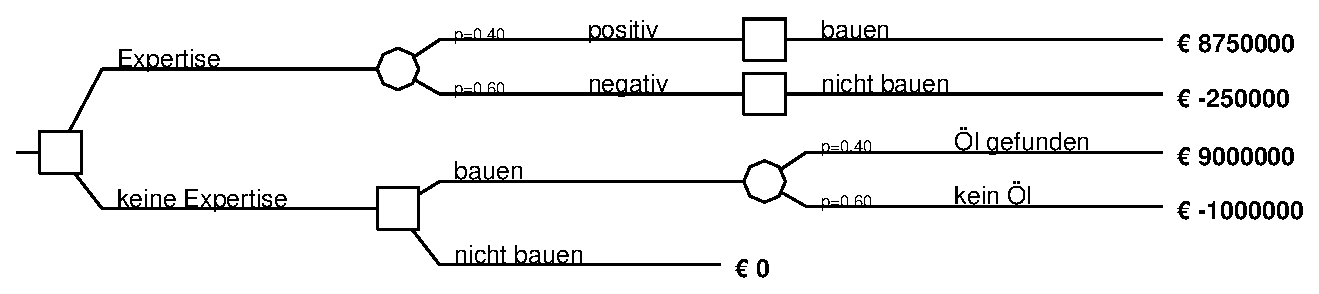
\includegraphics[width=12cm]{Grafiken/Beispiel6_3A.eps}
\end{center}
Wie kann man nun die Frage klären, ob es sich lohnt eine Expertise durchführen
zu lassen oder nicht? Dazu muss man den Entscheidungsbaum von rechts nach links
schrittweise nach folgenden Regeln auflösen:
\begin{enumerate}
  \item Ersetze jeden {\em Ereignis}knoten (der letzten Ebene) durch den
  Erwartungsnutzen des entsprechenden Ereignisses.\marginline{Regeln zur
  Auflösung von Entscheidungsbäumen}
  \item Ersetze jeden {\em Entscheidungs}knoten (der letzten Ebene) durch den
  (Erwartungs-)Wert der besseren Alternative.
  \item Führe das Verfahren fort bis die gesuchte (Teil-)Entscheidung erreicht
  ist.
\end{enumerate} 
In unserem Fall ist die gesuchte Entscheidung die Anfangsentscheidung, ob eine
Expertise durchgeführt werden soll. Wenn man den Baum nach dem entsprechenden
Verfahren reduziert, dann sieht der Entscheidungsbaum nach dem ersten Schritt
so aus:
\begin{center}
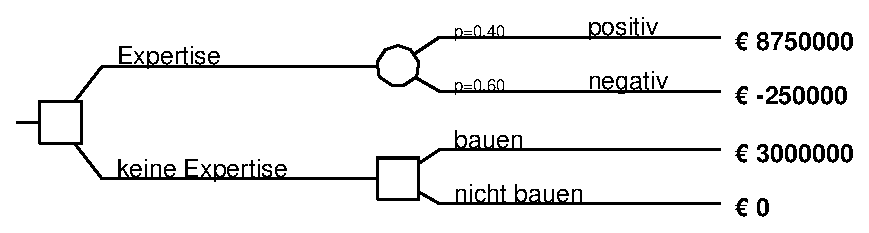
\includegraphics[width=10cm]{Grafiken/Beispiel6_3B.eps}
\end{center}
Der Erwartungswert, den man erhält, wenn man die Bohrinsel baut, ohne eine
Expertise durchzuführen beträgt € 3.000.000 (= € $0.4 \cdot 9.000.000 - 0.6
\cdot 1.000.000$). Dieser Erwartungswert wurde an die Stelle des entsprechenden
Ereignisknotens gesetzt. Da im anderen Fall die Entscheidung zum Bau
mit dem Ausgang der Expertise schon feststeht, wurden hier einfach die
entsprechenden Werte übertragen. Da der Bau der Ölplattform auch ohne vorherige
Probebohrung einen höheren Erwartungswert als 0 € liefert, muss für den letzten
Schritt nur noch der Erwartungsnutzen berechnet werden, der sich ergibt, wenn
man sich dazu entscheidet, die Expertise durchzuführen. Der nochmals reduzierte
Entscheidungsbaum sieht dann so aus:
\begin{center}
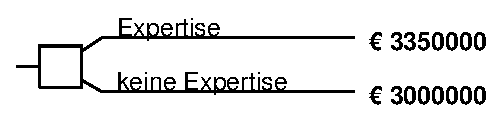
\includegraphics[width=6cm]{Grafiken/Beispiel6_3C.eps}
\end{center}
Es ist nun unmittelbar ersichtlich, dass es besser ist, vorher eine Expertise
in Auftrag zu geben, da der daraus resultierende Erwartungswert der größere
ist. 

Bei all diesen Beispielen haben wir übrigens eine Frage offen gelassen, die in
der praktischen Anwednung des Erwartungsnutzens von entscheidender Bedeutung
sein kann, nämlich die Frage, woher wir die Wahrscheinlichkeiten kennen, und ob
wir sicher sein können, dass die Wahrscheinlichkeiten für das Eintreten der
Ereignisse stimmen, wenn wir schon nicht sicher sein können, welches Ereignis
eintritt. Im Einzelfall dürfte dies von der Verfügbarkeit und Zuverlässigkeit
wissenschaftlicher Theorien abhängen, die diese Wahrscheinlichkeiten für den
entsprechenden Anwendungsbereich bestimmen.

\subsection{Die Rechtfertigung des Erwartungsnutzens}
\label{RechtfertigungErwartungsnutzen}
Soeben wurde gezeigt, wie man mit Hilfe des Erwartungsnutzens auf einfache
Weise Entscheidungsprobleme lösen kann. Zugleich wurde behauptet, dass der
Ewartungsnutzen bei Entscheidungen unter Risiko im Grunde die einzig sinnvolle
Entscheidungsregel darstellt. Aber warum ist das so? 

Eine Antwort auf diese Frage ist die, dass man, wenn man bei Entscheidungen unter
Risiko den Erwartungsnutzen zu Grunde legt, {\em auf lange Sicht} den größten
\marginline{Erwartungs\-nutzen ist auf lange Sicht gewinnmaximierend}
Gewinn erzielen kann.\footnote{Auch hier gibt es natürlich diskussionsbedürftige
Grenz- und Zweifelsfälle, wie z.B. \cite{okasha:2007} vor Augen führt.} Um sich
das klar zu machen nehme man eine Entscheidungssituation an, in der man entweder
einen festen Geldbetrag erhalten kann, oder mit einer bestimmten
Wahrscheinlichkeit einen höheren Geldbetrag. Z.B. könnte eine Person vor der
Entscheidung stehen, ob sie mit 5 € Einsatz an einer Lotterie teilnehmen will,
bei der sie mit 3\% Wahrscheinlichkeit 100 € gewinnen kann, oder ob sie das Geld
lieber behält. Behält sie das Geld, so entspricht das einem sicheren Gewinn von
5€. Wird diese Entscheidungssituation viele Male wiederholt, dann besagt das
Gesetz der Großen Zahlen aus der Statistik, dass der Grenzwert der Häufigkeit, mit der
ein bestimmtes Ereignis eintritt (in diesem Fall der Gewinn der Lotterie) mit der
Wahrscheinlichkeit 1 (also "`praktisch immer"') der Wahrscheinlichkeit des
Ereignisses entspricht. Handelt es sich bei der Wahrscheinlichkeit des Ereignisses um eine empirisch-statistische
Wahrscheinlichkeit und legt man die Häufigkeitstheorie der Wahrscheinlichkeit zu
Grunde (siehe Kapitel \ref{Haeufigkeitstheorie}), so gilt sogar, dass der
Grenzwert der Häufigkeit mit Sicherheit der Wahrscheinlichkeit des Ereignisses
entspricht.\footnote{"`Mit Sicherheit"' und "`mit Wahrscheinlichkeit 1"' ist
nicht, wie man denken könnte, ein- und dasselbe. Beispiel: Die Wahrscheinlichkeit
dafür, dass eine unendliche Folge von Münzwürfen nicht jedes mal Kopf liefert
befträgt 1. Trotzdem ist diese Ereignis nicht absolut sicher, denn das inverse
Ereignis, dass eine unendliche Folge von Münzwürden jedesmal Kopf liefert, ist
immerhin möglich.} Einfach ausgedrückt bedeutet dies: Wir können bei
hinreichend häufiger Wiederholung getrost davon ausgehen, dass das Ereignis genau so oft
eintritt, wie es seiner Wahrscheinlichkeit entspricht. In diesem Fall hieße das,
dass drei Prozent der Lotterien gewonnen werden. Bei einem Gewinn von 100 € wird
man auf lange Sicht 3 € pro Lotterie eingenommen haben, was genau dem
Erwartungswert der Lotterie $EU=0.03 \cdot 100$ € entspricht. Damit ist die
Lotterie aber deutlich weniger wert als der Einsatz von 5 €. Zumindest auf lange
Sicht sollte man immer den Erwartungswert (gleich Wahrscheinlichkeit mal
erwarteter Wert) für die Bewertung von Zufallsereignissen zu Grunde legen. Oder,
anders gesagt, man soll Zufallsereignisse weder zu optimistisch noch zu
pessimistisch bewerten, sondern genau entsprechend ihrer Wahrscheinlichkeit.

Dieselbe Argumentation lässt sich auch auf beliebige kardinale Nutzenwerte
übertragen, sofern man die Geldwerte durch Nutzenwerte ersetzt und statt des
Erwartungs{\em wertes} mit dem Erwartungs{\em nutzen} rechnet.

Die Argumentation weist zwei Schwierigkeiten auf: \marginline{Mögliche Einwände}
Erstens gilt sie nur auf lange Sicht, und es stellt sich zumindest die Frage, ob
man das, was auf lange Sicht gilt, auch auf einzelne Zufallsereignisse, die sich
in derselben Form nicht wiederholen, übertragen darf. Zweitens lässt sie sich --
wie schon erwähnt -- nur bei kardinalen Nutzenwerten anwenden, da wir sonst den
Erwartungsnutzen nicht einmal bestimmen können. Für beide Probleme versucht die
Neumann-Morgensternsche Nutzentheorie eine Lösung anzubieten. Für das erste
Problem, indem sie zeigt, dass der Erwartungsnutzen aus bestimmten
Konsistenzbedingungen hervorgeht, die verletzt werden, wenn man ihn nicht richtig
als das Produkt aus erwartetem Nutzen und Wahrscheinlichkeit berechnet -- ähnlich
wie subjektive Wahrscheinlichkeiten inkonsistent werden, sobald man die Axiome
der Wahrscheinlichkeitsrechnung verletzt (siehe
\ref{SubjektiveWahrscheinlichkeiten}). Für das zweite Problem, indem sie aus
einer beliebigen Präferenzrelation -- die aber reich genug sein muss, um auch
gedachte Güter von der Form sogenannter "`Lotterien"' zu enthalten! -- durch
trickreiche Vergleiche eine kardinale Nutzenfunktion konstruiert. Diese Theorie
werden wir später im Semester noch ausführlich besprechen (Kapitel
\ref{NeumannMorgenstern}).

\subsection{Kausale Entscheidungstheorie}

Bei einem der eben besprochenen Beispiele (Seite
\pageref{BeispielKausaleEntscheidung}) hingen die Wahrscheinlichkeiten, mit denen
Ereignisse eintreten, von den gewählten Handlungen ab.\footnote{Das
Hellseherparadox (Kapitel \ref{Hellseherparadox}) liefert ein weiteres, wenn
auch, da es echte hellseherische Fähigkeiten voraussetzt, sehr konstruiertes
Beispiel dafür.} Grundsätzlich werden solche Entscheidungsprobleme so gelöst,
dass wir die (handlungsabhängige) Wahrscheinlichkeit jedes möglichen Ergebnisses
in der entsprechenden Tabellenzelle vermerken und beim Ausrechnen des
Erwartungsnutzens für jede Handlung die in der entsprechenden Zeile vermerkten
Wahrscheinlichkeiten berücksichtigen.

Wir können nun noch einen Schritt weitergehen und uns fragen, wie vorzugehen
ist, wenn die Wahrscheinlichkeiten des Eintretens von Ereignissen nicht nur von den
Handlungen sondern wiederum von anderen Ereignissen und Zuständen abhängig sind.
Dazu ein Beispiel (frei nach Resnik \cite[S. 114]{resnik:1987}): Eine Ärztin
steht vor der Frage, ob sie die Infektion eines Patienten mit einem
Desinfektionsmittel oder mit einem Antibiotikum behandeln soll. Das
Antibiotikum schlägt bei 80\% der Patienten gut an, in welchem Fall die
Heilungschance bei 70\% liegt. Bei den restlichen Patienten liegt die
Heilungschance mit demselben Mittel jedoch nur bei 40\%. Das
Desinfektionsmittel hat dagegen bei allen Patienten eine Heilungschance von 50\%
Da beide Mittel, wie wir einmal annehmen wollen miteinander unverträglich sind,
besteht nur die Wahl entweder das Antibiotikum zu versuchen oder das
Desinfektionsmittel.

Um das Problem in einer Entscheidungstabelle darzustellen, kann man die
Ereignisse in zwei Gruppen unterteilen: Unabhängige und Abhängige Ereignisse. In
diesem Fall ist das unabhängige Ereignis, dasjenige, ob das Antibiotikum bei dem
Patienten anschlägt oder nicht. Das kausal davon abhängige Ereignis ist die
Heilung (oder Nicht-Heilung) des Patienten. Dabei müssen für jedes unabhängige
Ereignis alle abhängigen Ereignisse gesondert eingetragen werden. Wichtig ist,
dass man innerhalb der Tabelle die entsprechenden bedingten Wahrscheinlichkeiten
einträgt. Daraus ergibt sich folgende Entscheidungstabelle:
\begin{center}
\begin{footnotesize}
\begin{tabular}{c|c|c|c|c|}
\multicolumn{1}{c}{} & \multicolumn{2}{c}{A. schlägt an (80\%)} 
                     & \multicolumn{2}{c}{schlägt nicht an (20\%)} \\
\multicolumn{1}{c}{} & \multicolumn{1}{c}{Heilung (70\%)}
                     & \multicolumn{1}{c}{$\neg$Heilung (30\%)}
                     & \multicolumn{1}{c}{Heilung (40\%)}
                     & \multicolumn{1}{c}{$\neg$Heilung (60\%)}
                     \\ \cline{2-5}                       
Antibiotikum  & gesund (56\%) & krank (24\%) & gesund (8\%) & krank (12\%) 
\\ \cline{2-5} 
Des.-Mittel   & gesund (40\%) & krank (40\%) & gesund (10\%) & krank (10\%) 
\\ \cline{2-5}
\end{tabular}
\end{footnotesize}
\end{center}
Wie man sieht, wäre bei diesem Beispiel die Heilungschance mit dem
Antibiotikum (56\% + 8\% = 64\%) größer als mit dem Desinfektionsmittel (40\%
+ 10\% = 50\%). Sind bei einem Entscheidungsproblem wie diesem die
Kausalzusammenhänge zwischen Ereignissen und Handlungen zu berücksichtigen, bietet sich oft die anschaulichere
Baumdarstellung an.


\subsection{Entscheidungsregeln in der Philosophie: Die Debatte zwischen John
Rawls und John C. Harsanyi}
\label{RawlsHarsanyiDebatte}

Zum Abschluss des Teils über "`Techniken des Entscheidens"' soll ein Beispiel aus
der Philosophie erörtert werden, das vor Augen führt, wie technische Fragen der
Entscheidungstheorie auch in die philosophische Diskussion hineinspielen können. 
Bei diesem Beispiel kommen besonders die Maximin-Regel und das Prinzip der
Indifferenz zum Tragen.

 Die Maximin-Regel hat in der Philosophie einige
Bekanntheit erlangt, weil sie an prominenter Stelle in John Rawls sehr
einflussreichem Werk "`Eine Theorie der Gerechtigkeit"' auftaucht. John Rawls
vertritt in diesem Werk den Grundsatz, dass dasjenige Gesellschaftsmodell das
gerechteste ist, in dem es den am schlechtesten gestellten Menschen im Vergleich
mit anderen Modellen am besten geht. Etwas anders formuliert könnte man auch
sagen, dass Ungleichheit nur insoweit gerechtfertigt ist, wie sie {\em jedermann}
zum Vorteil gereicht \cite[S. 96ff.]{rawls:1971}.\marginline{Rawls'
Differenzprinzip} Dieses Prinzip wird auch das "`Differenzprinzip"' genannt.
Rawls stellt diesem Prinzip noch das von Kant übernommene "`Freiheitsprinzip"'
voran, wonach in der Gesellschaft jeder Mensch soviel Freiheit genießen soll wie
möglich ist, sofern seine Freiheit mit demselben Maß an Freiheit für
andere Menschen noch verträglich sein soll. Unfreie Gesellschaften kommen also
von vornherein nicht als gerechte Gesellschaften in Betracht. Uns soll hier aber
nur das Differenzprinzip interessieren.

Rawls liefert in seinem Werk für das Differenz\-prinzip eine
Quasi-\-Ab\-leit\-ung, für die er sich der in der vertragstheoretischen
Tradition seit Hobbes beliebten Vorstellung eines Urzustandes bedient. Rawls
stellt sich einen hypothetischen Urzustand vor, in dem die Menschen ein
Gesellschaftsmodell wählen dürfen. In diesem Urzustand wissen sie aber noch
nicht, welche (soziale) Rolle sie in der gewählten Gesellschaft einnehmen werden.
Sie befinden sich hinter einem {\em Schleier des Nichtwissens}. Welche
Gesellschaft werden sie in einer solchen Situation wohl wählen? An dieser Stelle
kommt die Maximin-Regel ins Spiel. Denn Rawls ist überzeugt davon, dass in einer
solchen Situation die einzige Entscheidungsregel, deren sich ein vernünftiger
Mensch bedienen würde, die Maximin-Regel ist. (Wenn es um das eigene
Lebensschicksal geht, dann sollte man besser auf Nummer sicher gehen.) Nach der
Maximin-Regel würden die Menschen aber die Gesellschaft wählen, die nach dem
Differenzprinzip die Gerechteste ist, denn das ist genau die Gesellschaft, in er
es einem im schlimmsten Fall noch am besten geht.

\marginline{Harsanyis utilitaristischer Gegenstandpunkt}
Harsanyi vertritt dazu den utilitaristischen Gegenstandpunkt: Seiner Ansicht nach
muss eine rationale Entscheidungsregel auf dem Prinzip der Indifferenz beruhen
und statt der Maximin-Regel den Durchschnittsnutzen heranziehen unter der Annahme
der Gleichverteilung aller möglichen Ergebnisse. Er rechtfertigt dies einmal mit
offensichtlichen Konsistenzbedingungen wie z.B. der Transitivität der Präferenzen
oder dem Prinzip „Du wirst besser gestellt sein, wenn Du [in einer Lotterie]
einen höheren Gewinn mit einer gegebenen Wahrscheinlichkeit angeboten bekommst,
als wenn Du einen niedrigeren Gewinn mit der gleichen Wahrscheinlichkeit
angeboten bekommst“ \cite[S. 47]{harsanyi:1975}, von denen man in der Tat
mathematisch zeigen kann, dass wenigstens einige davon verletzt werden, wenn man
vom Durchschnittsnutzen abweicht. Eine nicht unwichtige Voraussetzung ist dabei
aber, dass Harsanyi hinter dem Schleier des Nichtwissens entsprechend dem
Indifferenzprinzip eine Gleichverteilung der möglichen individuellen Rollen
annimmt.\footnote{Das ist so zu verstehen: Angenommen in der Gesellschaft, für
die die Verfassung gefunden werden soll, gibt es 1 Mio Individuen, dann muss der
Einzelne nach dem Indifferenzprinzip annehmen, dass er mit gleicher
Wahrscheinlichkeit jedes dieser Individuen sein könnte. Wenn wir also eine
Verfassung betrachten, bei der 99\% der Menschen in Armut leben und 1\% in
Reichtum, so muss der Einzelne annehmen, dass er mit 99\% Wahrscheinlichkeit die
Rolle eines der Armen übernehmen wird. Insofern hängt das Gewicht einer
bestimmten gesellschaftlichen Klasse bei Harsanyi auch von ihrer Größe ab.}
Zusätzlich führt Harsanyi noch einige Einzelbeispiele in Form von Gedankenexperimenten an,
in denen die Maximinregel unplausibel erscheint, wie z.B.: „Du kannst
in Chicago einen super Job bekommen, oder zu Hause bei Deinem miesen Job bleiben.
Wenn Du nach Chicago fliegst, könnte das Flugzeug natürlich abstürzen...“ Nach
der Maximin-Regel müsste man zu Hause bleiben, was Harsanyi absurd findet.

Um den Unterschied der beiden Positionen in Bezug auf die Frage der
Gerechtigkeit zu verdeutlichen, können wir uns als Beispiel \cite[S.
41]{resnik:1987} zwei mögliche Gesellschaftsmodelle denken. In dem ersten
Gesellschaftsmodell arbeiten 10\% der Menschen hart, damit die
restlichen 90\% wohlleben können. Die 10\% Arbeiter erhalten jeweils
einen (kardinalen) Nutzen von 1, die anderen von 90, macht im Schnitt
81,1. In einem anderen Gesellschaftsmodell
muss sich jeder an der Arbeit beteiligen, und jeder erzielt einen
Nutzen von 35. Für welche Gesellschaft würden sich die Menschen
hinter einem {\em Schleier des Nichtwissens} entscheiden? Mit Rawls
und dem Maximin-Prinzip für die zweite. Mit Harsanyi und dem
Utilitarismus für die erste.

\marginline{Mögliche Rekonstruktionen von Rawls' Theorie}
Wie sind die unterschiedlichen Positionen zu beurteilen? Kann Harsanyi Rawls
Gerechtigkeitstheorie mit Hilfe der Entscheidungstheorie wiederlegen? Die
Beantwortung dieser Frage hängt sehr stark davon ab, wie man die
Gerechtigkeitstheorie von Rawls und insbesondere ihre Begründungslogik
rekonstruiert. Es gibt – stark vereinfacht – zwei Möglichkeiten das zu tun:

\begin{enumerate}
\item \marginline{1. Ethische Rekonstruktion} 
  Man siedelt die {\em ethische Basisentscheidung} auf der Ebene
  des Gerechtigkeitsprinzips selbst an. Dann muss man zunächst die
  Entscheidung (im {\em dezisionistischen}, nicht im
  entscheidungstheoretischen Sinne!) treffen, ob man das
  Differenzprinzip oder den Utilitarismus als Gerechtigkeitsprinzip
  wählen möchte. Alle Schlussfolgerungen, die man dann aus dem
  gewählten Prinzip in Bezug auf den Aufbau und die Institutionen der
  gerechten Gesellschaft zieht, sind dann ethische Deduktionen. All
  dasjenige, {\em woraus} man umgekehrt das gewählte Gerechtigkeitsprinzip
  ableiten könnte, also insbesondere alle Urzustandsszenarien, sind dann
  lediglich begründende Mythen, deren berechtigter Zweck allein darin
  besteht, das Gerechtigkeitsprinzip zu motivieren, erzählerisch
  auszuschmücken, propagandistisch aufzuwerten usf.

  Sollte sich nun durch eine entscheidungstheoretische Kritik wie der von
  Harsanyi zeigen, dass das gewählte Gerechtigkeitsprinzip nicht aus dem
  Urzustand ableitbar ist, dann beweist das bestenfalls, dass man auf einen
  ungeeigneten Mythos zurückgegriffen hat, um es zu motivieren. Andererseits
  beruht aber gerade die Kritik von Harsanyi auf dem Nachweis der Verletzung von
  Konsistenzbedingungen durch die von Rawls für die Entscheidung im Urzustand
  reklamierte Maximin-Regel. Nun kann man aber ernsthaft fragen, ob es für das
  Urzustandsszenario, zumal wenn es ohnehin keine begründende Bedeutung hat, auf
  die Konsistenz und Rationalität (im dem engen Sinne, in dem Harsanyi den
  Ausdruck Rationalität gebraucht) der Entscheidung überhaupt ankommt. Rawls
  beansprucht freilich, dass eine Entscheidung nach der Maximin-Regel im
  Urzustand eine vernünftige Entscheidung ist. Aber schlimmstenfalls wäre er
  nur gezwungen seinen Urzustandsmythos fallen zu lassen oder durch einen
  anderen zu ersetzen, nicht jedoch dazu, das Differenzprinzip aufzugeben.

\item \marginline{2.~Meta-ethische Rekonstruktion} 
  Man siedelt die ethische Basisentscheidung auf der Ebene des
  Urzustandes oder sogar davor an, so dass diejenige Gesellschaftsordnung als
  gerecht gelten muss, die sich daraus ableiten lässt. In gewisser Weise scheint
  die Basisentscheidung, zumindest was Harsanyi betrifft, noch vor dem Urzustand
  zu liegen, indem er als wesentliches Merkmal des Moralischen vorauszusetzen
  scheint, dass man von den Interessen, die man als konkretes Einzelindividuum
  hat absieht und die Interessen der anderen gleichwertig mitberücksichtigt. Das
  motiviert dann die Konstruktion des Urzustandes hinter dem Schleier des
  Nichtwissens. (Eine Konstruktion von der Harsanyi beansprucht, dass er sie
  unabhängig von Rawls schon herangezogen hat.) Außer dieser recht formalen
  Bedingung für Moral scheint Harsanyi weitere, konkrete ethische Entscheidungen
  (im Sinne von Dezisionen) nicht zuzulassen.

  Nur in diesem zweiten Fall kommt der entscheidungstheoretischen
  Argumentation tatsächlich eine Schlüsselfunktion zu. Denn einmal den
  Urzustand als ethische Basisentscheidung gegeben, hängt es von der
  korrekten Anwendung der entscheidungstheoretischen Regeln ab,
  welches Gesellschaftsmodell als das gerechteste betrachtet werden
  muss. Harsanyis Kritik ist an Rawls Gerechtigkeitsideal ist dann in
  dem Maße berechtigt wie seine Kritik der Maximin-Regel zutrifft.

\end{enumerate}


Was ist zu dieser Kritik zu sagen? Zunächst, was die Einzelbeispiele betrifft,
mit denen Harsanyi gegen die Maximin-Regel polemisiert:
\marginline{Beispiele gegen den Utilitarismus}
Gegen den Utilitarismus kann man ebensogute Einzelbeispiele anführen, z.B.: Ein
Mensch ist todkrank und kann nur durch eine Spenderniere gerettet werden. Da sich
kein Spender findet, ordnet die Regierung an, einem, der als Spender in Frage
käme, zwangsweise eine Niere zu entnehmen. Aus utilitaristischer Sicht ist das
Handeln der Regierung sehr zu loben, da die Gesamtnutzenbilanz: Gerettetes Leben des
einen abzüglich des körperlichen Schaden des anderen positiv ausfällt. (Das
Beispiel verweist auf ein Grundproblem des Utilitarismus, nämlich dessen
Unfähigkeit {\em unveräußerliche Rechte} wie z.B. ein Recht auf körperliche
Unversehrtheit) zu begründen. Oder: Auf einer Insel ist eine Gruppe von Leuten
gestradet. Die Rettung ist unterwegs, verzögert sich aber und wird erst
eintreffen, wenn schon alle verhungert sind. Wenn nun aber die eine Hälfte der
Gruppe die andere schlachtet und verspeist, kann wenigstens die Hälfte bis zum
eintrffen der Rettung überleben. Utilitaristisch und unter dem Gesichtspunkt des
Durchschnittsnutzens betrachtet, ist es besser, wenn die Hälfte überlebt als wenn
alle sterben und der Kannibalismus damit zur moralischen Pflicht erhoben\ldots
Kurz, mit Einzelbeispielen kann man jedes Moralprinzip kleinkriegen. (Das zeigt
weder, dass Einzelbeispiele noch dass allgemeine Moralprinzipien falsch sind,
aber vielleicht, dass man nicht mit einem einzigen einfachen Moralprinzip
auskommt, und dass in der Moral wie im Leben ein gewisses Maß an Inkonsequenz
empfehlenswert ist.)

\marginline{Reichweite des Inkonsistenzvorwurfs}
Ernstzunehmender ist die Kritik, soweit sie sich auf die Verletzung von
elementaren Konsistenzbedingungen durch die Maximin-Regel bezieht. Allerdings
setzt Harsanyi bei seiner Kritik {\em kardinale} Nutzenbewertungen für die
sozialen Rollen voraus, die die Individuen in unterschiedlichen Gesellschaftsmodellen
einnehmen \cite[S. 48f.]{harsanyi:1975}. Zudem geht er von der Gültigkeit der
Erwartungsnutzenhypothese (siehe Kapitel \ref{Erwartungsnutzenhypothese}, Seite
\pageref{Erwartungsnutzenhypothese}) aus. Ohne auf die Problematik des {\em
kardinalen Nutzens} an dieser Stelle schon einzugehen (siehe dazu Kapitel
\ref{DiskussionNeumannMorgenstern}, Seite
\pageref{DiskussionNeumannMorgenstern}), ist anzumerken, dass die Voraussetzungen
für die Anwendung eines derart starken Nutzenkonzepts in dem vorliegenden
Gedankenexperiment kaum gegeben sein dürften. Auch der Rückgriff auf den
Erwartungsnutzen ist, da es sich um ein einmaliges Ereignis handelt, mit
Einschränkungen fragwürdig. Die Anwendung des Indifferenzprinzips führt 
hier zwar nicht zu Paradoxien, da man einigermaßen schlüssig davon ausgehen kann,
dass wir es auf die Wahrscheinlichkeit beziehen, jeweils eine bestimmte
individuelle Rolle zu übernehmen. Aber da die Annahme jeder anderen
Wahrscheinlichkeitsverteilung genauso legitim wäre, kann Harsanyi an Rawls'
Ansatz nicht legitimerweise kritisieren, dass dabei implizit eine sehr
unausgewogene Wahrscheinlichkeitsverteilung angenommen wird. (Ohne das
Indifferenzprinzip lassen sich die dem Rawls'schen Ansatz vorgeworfenen
Inkonsistenzen aber immer durch eine entsprechende
Wahrscheinlichkeitsverteilung auffangen.)

\marginline{Harsanyis dogmatischer Szientismus}
Schließlich sei noch angemerkt – aber dies ist zugegebenermaßen mehr ein
Vorbehalt – dass es bei Harsanyi manchmal so erscheint, als ob er den
Utilitarismus nur auf Grund einer idiosynkratischen Vorliebe für ein Moralsystem
bevorzugt, das sich am ehesten mit der von ihm offenbar geschätzten Stilform
eines (wahrscheinlichkeitstheoretischen) Kalküls verbinden lässt, ohne dass er
die dabei zu treffenden sittlichen Entscheidungen überhaupt bewusst als
solche reflektiert. In der Einleitung seiner Rawls-Kritik lässt er die Bemerkung
fallen, dass der Utilitarismus „up to now in its various forms was virtually the
only ethical theory proposing a reasonably clear, systematic and purportedly
rational concept of morality“ \cite[]{harsanyi:1975} sei, als ob das die einzigen
oder gar wichtigsten Maßstäbe wären, nach denen man die Entscheidung für oder
gegen ein Moralsystem treffen müsste, und nicht vielmehr in erster Linie dessen
sittlicher Gehalt! Sofern man die Kriterien "`reasonably clear, systematic and
purportedly rational"' nicht von vornherein in einem so engen Sinne versteht,
dass seine Behauptung, dass nur der Utilitarismus sie erfülle, tautologisch
wird, dürfte diese Behauptung philosophiehistorisch gesehen ohnehin schlichtweg
falsch sein.



\newpage
\subsection{Aufgaben}
\begin{enumerate}
  
  \item Zeige durch ein Beispiel, dass der berechnete Erwartungsnutzen
  sich bei gleichbleibenden Präferenzen ändern kann, wenn man bloß von einem
  {\em ordinalen Nutzen} ausgeht. M.a.W.: Um den Erwartungsnutzen sinnvoll
  einsetzen zu können, müssen wir immer das vergleichsweise stärkere aber
  empirisch schwerer zu rechtfertigende Konzept des {\em kardinalen Nutzens}
  voraussetzen.
  
  \item Stelle das folgende Entscheidungsproblem aus der Vorlesung (Seite
  \pageref{RisikoBeispiel1}) als Entscheidungsbaum dar und löse den
  Entscheidungsbaum schrittweise auf.

\begin{center}
\begin{tabular}{c|r|r|r|r}
\multicolumn{1}{c}{}  & \multicolumn{1}{c}{$S_1$ ($p=0.3$)}  &
\multicolumn{1}{c}{$S_2$ ($p=0.2$)} & \multicolumn{1}{c}{$S_3$ ($p=0.5$)} \\
\cline{2-4} $A_1$ & -100.000 € & -50.000 & € 60.000 & $EU = -10.000$ €\\ 
\cline{2-4} $A_2$ & 0 €        & -80.000 & € 0      & $EU = -16.000$ €\\ 
\cline{2-4}
\end{tabular}
\begin{small}
\begin{tabular}{llp{10cm}}
& & \\
$A_1$ & & Investiere in die rasche Entwicklung eines Kleinstlaptops.\\
$A_2$ & & Investiere nicht in die Entwicklung eines Kleinstlaptops.\\
& &\\
$S_1$ & & Kleinstlaptops bleiben auf dem Markt erfolglos.\\
$S_2$ & & Kleinstlaptops sind erfolgreich, aber die Konkurrenz
                   ist ebenfalls frühzeitig auf dem Markt präsent.\\
$S_3$ & & Kleinstlaptops sind erfolgreich, aber die Entwicklung 
                   der Konkurrenz verzögert sich. \\
\end{tabular}
\end{small}
\end{center}
  
 \item {\em Stelle das folgende Entscheidungsproblem als Entscheidungsbaum} dar:
  Eine Ärztin steht vor der Frage, ob sie die Infektion eines Patienten mit einem
Desinfektionsmittel oder mit einem Antibiotikum behandeln soll. Das Antibiotikum
schlägt bei 80\% der Patienten gut an, in welchem Fall die Heilungschance bei
70\% liegt. Bei den restlichen Patienten liegt die Heilungschance mit demselben
mittel jedoch nur bei 40\%. Das Desinfektionsmittel hat dagegen bei allen
Patienten eine Heilungschance von 50\% Da die Mittel miteinander unverträglich
sind, besteht nicht die Möglichkeit beide Mittel zu verabreichen.

\begin{center}
\begin{scriptsize}
\begin{tabular}{c|c|c|c|c|}
\multicolumn{1}{c}{} & \multicolumn{2}{c}{A. schlägt an (80\%)} 
                     & \multicolumn{2}{c}{schlägt nicht an (20\%)} \\
\multicolumn{1}{c}{} & \multicolumn{1}{c}{Heilung (70\%)}
                     & \multicolumn{1}{c}{$\neg$Heilung (30\%)}
                     & \multicolumn{1}{c}{Heilung (40\%)}
                     & \multicolumn{1}{c}{$\neg$Heilung (60\%)}
                     \\ \cline{2-5}                       
Antibiotikum  & gesund (56\%) & krank (24\%) & gesund (8\%) & krank (12\%) 
\\ \cline{2-5} 
Des.-Mittel   & gesund (40\%) & krank (40\%) & gesund (10\%) & krank (10\%) 
\\ \cline{2-5}
\end{tabular}
\end{scriptsize}
\end{center}
  
\item Wie kann man die Wahl eines Gesellschaftsmodells hinter einem Rawlsschen
{\em Schleier des Nichtwissens} als Entscheidungstablle darstellen? Und als
Entscheidungsbaum?  

\end{enumerate}




\chapter{Zur Theorie der Kollektiven Entscheidungen}

\section{Sozialwahltheorie}
\label{Sozialwahltheorie}

Bisher haben wir uns nur mit individuellen Entscheidungen beschäftigt. Für die
Anwendung der Theorie ist es dabei weniger wichtig, ob die Akteure bzw.
"`Agenten"' tatsächlich einzelne Individuen sind, oder ob sie etwa Gruppen oder
Körperschaften sind. Entscheidend ist, dass sie über eine ganz bestimmte
Präferenzrelation verfügen, die die Bedingungen für Präferenzrelationen erfüllt,
also Ordnung, Transitivität etc. (siehe Kapitel \ref{Praeferenzen}, ab Seite
\pageref{Praeferenzen}). \marginline{kollektive Entscheidungen} Die
Sozialwahltheorie beschäftigt sich nun genau mit der Frage, wie eine Gruppe von
Individuen kollektive Entscheidungen treffen kann, wenn man noch nicht von
vornherein eine kollektive Präferenzrelation als gegeben betrachtet. Man könnte
auch sagen, dass das Problem bzw. eines der Hauptprobleme der Sozialwahltheorie
darin besteht, wie man individuelle Präferenzen auf kollektive Präferenzen
abbilden kann. Um ein Problem handelt es sich insofern, als die individuellen
Präferenzen einer Gruppe von Menschen höchst unterschiedlich beschaffen sein
können, selbst wenn man einmal annimmt, dass jedes Mitglied der Gruppe über eine
im Sinne der Theorie gültige Präferenzrelation verfügt. Wie wir sehen werden,
kann es zu Schwierigkeiten kommen, wenn man daraus eine kollektive
Präferenzrelation ableiten will, die immer noch die Bedingungen einer
wohlgeordneten Präferenzrelation erfüllt.

Die individuellen Präferenzen sämtlicher Individuen zusammengenommen, bezeichnet
man auch als "`{\em Präferenzprofil} "'. Ein Präferenzprofil ist also eine Menge
von individuellen Präferenzrelationen.\marginline{soziale Wohlfahrtsfunktion} Die
Abbildung des Profils von individuellen Präferenzrelationen auf eine einzelne
kollektive Präferenzrelation nennt man eine "`{\em soziale Wohlfahrtsfunktion}"'
oder, im Zusammenhang der Entscheidungstheorie, auch ein "`{\em
Kollektiventscheidungsverfahren}"'. Mathematisch betrachtet haben wir es dabei mit
folgenden Gegenständen zu tun:

\begin{enumerate}
  \item Mit einer Menge ${\cal X} = \{x, y, z, \ldots\}$ von Alternativen oder
  Güterbündeln, die jeweils mit kleinen Buchstaben bezeichnet werden. Die Menge
  aller auf ${\cal X}$ möglichen Präferenzrelationen soll mit ${\cal R}$
  bezeichnet werden. (Für die definierenden Eigenschaften einer gültigen
  Präferenzrelation siehe \pageref{Ordnungsaxiome}.)
 
  \item Mit einer bestimmten Anzahl von Individuen $A, B, C, \ldots$, die mit
  Großbuchstaben vom Anfang des Alphabets bezeichnet werden. Die Individuen kann
  man sich durchnummeriert denken, so dass man sinnvollerweise statt von $A$, $B$ oder
  $C$ auch vom ersten, zweiten oder dritten Individuuem oder ganz allgemein vom
   "`$i$-ten Individuuem"' sprechen kann.
  
  \item Mit individuellen Prä\-fer\-enz\-re\-la\-tion\-en, wobei jedes
  Individuum na\-tür\-lich eigene Prä\-fer\-enz\-en hat. Um anzuzeigen, wessen
  Präferenzen gemeint sind, kann man einen Index an das Präferenzzeichen
  anhängen, d.h. $x \succ_i y$, bedeutet, dass das $i$-te Individuum $x$
  gegenüber $y$ vorzieht. Die gesammte Präferenzrelation eines Individuums kann
  man mit $R_i$ bezeichnen.
 
  \item Mit einer kollektiven Prä\-fer\-enz\-re\-la\-tion, d.i. diejenige 
  Prä\-fer\-enz\-re\-la\-tion, die später für das Kollektiv gelten soll, und
  die, solange nichts Näheres darüber bestimmt ist, völlig unabhängig von den
  individuellen Präferenzen ist. Um zu kennzeichnen, dass kollektive Präferenzen gemeint
  sind, wird der Index $K$ an das Präferenzzeichen angehängt, also etwa
  $x \succ_K y$. Die gesamte kollektive Präferenzrelation wird wiederum mit
  $R_K$ bezeichnet.
   
  \item Mit Profilen von individuellen Präferenzen. Ein Profil ist dabei ein
  Tupel von individuellen Präferenzrelationen, in der für jedes Individuum
  genau eine Präferenzrelation $R_i$ festgelegt ist. Wenn wir ein
  beliebiges Präferenzprofil mit $P$ bezeichnen, dann gilt $P =
  (R_1,\ldots, R_n)$. Zwei Präferenzprofile $P_1, P_2$
  unterscheiden sich dann, wenn mindestens ein Individuum in $P_1$ andere 
  Präferenzen hat als in $P_2$.
  (Und es hat andere Präferenzen, wenn es wenigstens bezüglich eines Paars von 
  Alternativen eine andere Ordnung vornimmt.)
  
  \item Mit der Menge aller möglichen Präferenzprofile ${\cal P}$, die, wie der
  Name schon sagt, jedes nur denkbare Profil von wohlgeordneten
  individuellen Präferenzen enthält.
\end{enumerate}

Eine {\em Kollektiventscheidungsverfahren}\marginline{mathematische Definition}
 (auch "`soziale"' bzw.
"`ge\-sell\-schaft\-liche Wohl\-fahrts\-funk\-tion"' oder einfach
"`Sozialwahlfunktion"') ist nun eine Funktion $f: {\cal P} \mapsto {\cal R}$,
die jedem Präferenzprofil $P \in {\cal P}$ eine "`kollektive"' Präferenzrelation
$R_K \in {\cal R}$ zuordnet. Man kann auch schreiben: $f(P_1,\ldots, P_n)
= R_K$, wobei $(P_1,\ldots, P_n)$ ein bestimmtes Präferenzprofil ist, und
$R_K$ diejenige Präferenzrelation, die diesem Profil durch die
Sozialwahlfunktion $f$ zugeorndet wird.

Mit Hilfe dieses technischen Apparats kann die Frage untersucht werden, welche
Entscheidungs- bzw. Abstimmungsprozeduren zum Treffen von Kollektiventscheidungen
geeignet sind. Z.B. kann man damit die Frage untersuchen, ob die Entscheidung
nach dem demokratischen Mehrheitsprinzip zu effizienten, gerechten und
konsequenten Kollektiventscheidungen führt. Dazu müssen die entsprechenden
Anforderungen an eine Sozialwahlfunktion (Effizienz, Gerechtigkeit etc.)
natürlich zunächst mathematisch umschrieben werden. In diesem Zusammenhang ist es
wichtig darauf hinzuweisen, dass die Sozialwahltheorie keineswegs die einzige
Theorie ist, die sich mit diesen Fragen beschäftigt. Vielmehr werden die
entsprechenden Fragen in der politischen Philosophie schon seit der Antike
thematisiert, und schon längst bevor es die Sozialwahltheorie als eigenes
Fachgebiet gab, sind auf viele der von ihr untersuchten Probleme praxistaugliche
Lösungen gefunden worden. Was die Sozialwahltheorie von früheren Ansätzen
unterscheidet ist der formale mathematische Rahmen, in dem sie diese Probleme
untersucht.\marginline{Grenzen der Sozialwahltheorie} Leider erweist sich dieser
formale Rahmen nicht immer als ein Vorteil, indem viele wichtige Probleme und
Fragestellungen, die im Zusammenhang mit kollektiven Entscheidungsprozessen
stehen, sich innerhalb dieses Rahmens entweder überhaupt nicht oder nicht adäquat
artikulieren lassen. Die Sozialwahltheorie gibt nur einen ganz bestimmten
Blickwinkel auf solche Phänomene wie das der demokratischen Mehrheitsentscheidung
frei. Was z.B. weitgehend ausgespart bleibt, sind sogenannte "`deliberative"'
Prozesse, also diejenigen Vorgänge, in denen sich -- in der ökonomistischen
Sprache formuliert -- die Präferenzen der Individuen in Folge von öffentlichen
Diskussionen veränderen, aneinander anpassen oder sich dissozieren und in Lager
aufteilen. Und in einer nicht ökonomistischen Sprache formuliert, sind
deliberative Prozesse all diejenigen Diskussions- und Meinungsbildungsprozesse,
die, besonders in Demokratien, politischen Entscheidungen oder Abstimmungen
voraus zu gehen pflegen. Will man ein richtiges und vollständiges Bild von der
Natur demokratischer politischer Entscheidungsprozesse gewinnen, so ist die
Sozialwahltheorie allein dafür völlig unzureichend und sollte unbedingt durch
andere Theorien, z.B. solche, die deliberative Prozesse zum Gegenstand haben,
ergänzt werden. Zur klassischen politischen Philosophie steht die
Sozialwahltheorie also bestenfalls im Verhältnis einer Ergänzung. Keineswegs
handelt es sich dabei um eine "`streng wissentschaftliche"' Alternative, die die
traditionelle politische Philosophie ablösen oder ersetzen könnte.

\subsection{Zum Einstieg: Das Condorcet-Paradox}
\label{condorcetParadox}
Der grundlegende Widerspruch, auf dem in der ein- oder anderen Form viele der
Unmöglichkeitsbeweise der Sozialwahltheorie aufbauen, lässt sich beispielhaft
am sogenannten Condorcet-Paradox erläutern. Angenommen, wir haben drei
Individuen $A$,$B$, $C$, die über drei Alternativen
$x$,$y$,$z$ abstimmen wollen. Alle Individuen sind dabei gleichberechtigt. Ihre
Präferenzen sind folgendermaßen verteilt:

\begin{center}
\begin{tabular}{ccc}
\label{condorcetParadoxTabelle}
$A$ & $B$ & $C$ \\
\cline{1-3}
$z$ & $x$ & $y$ \\
$x$ & $y$ & $z$ \\
$y$ & $z$ & $x$ \\
\end{tabular}
\end{center}

Welche Alternative sollte gewählt werden? Jede Alternative steht einmal an
erster, einmal an zweiter und einmal an dritter Stelle. Man kann also keine
Alternative ohne Weiteres als die kollektiv beste auszeichnen, wenn man nicht
eines der Individuen in ungerechter Weise bevorzugen will. Das Problem lässt sich
auch nicht einfach verfahrenstechnisch lösen. Denn wollte man zum Beispiel
Stichwahlen durchführen, so würde im ersten Wahlgang jede Alternative die gleiche
Stimmenzahl erhalten, so dass man keine Alternative für den zweiten Wahlgang
ausschließen könnte. Wollte man paarweise Stichwahlen durchführen, so ergibt sich
jeweils, dass $x \succ_K y$, $y \succ_K z$, aber ebenso auch $z \succ_K x$. Bei
jedem dieser Paare wird ja das vordere Glied von jeweils zwei Individuen
bevorzugt.\marginline{Condorcet-Kriterium} Man nennt den Mechanismus von
paarweisen Stichwahlen zur Bestimmung der bevorzugten Alternative aus einer Menge
von Alternativen über die mehrere Individuen (möglicherweise) unterschiedliche
Präferenzen haben auch {\em Condorcet-Kriterium} (nach dem Marquis des Condorcet,
einem französischen Philosphen und Mathematiker des 18. Jahrhunderts, der dieses
Kriterium vorgeschlagen hat). Das Condorcet-Kriterium zur Bestimmung der
kollektiven Präferenzen würde also zu {\em zyklischen Präferenzen} führen, weil
$x \succ_K y \succ_K z \succ_K x$ gilt. \marginline{zyklische Präferenzen} Damit
wäre aber die Transitivität der kollektiven Präferenzrelation verletzt. Nun haben
wir zwar gesehen, dass intransitive Präferenzen keineswegs "`unnatürlich"' sein
müssen (siehe Seite \pageref{intransitivePraeferenzen}). Das vorliegende Beispiel
zeigt ja gerade, dass sie auf eine ganz natürliche und naheliegende Weise
(paarweise Stichwahlen) zustande kommen können. Aber intransitive Präferenzen
werfen trotzdem sowohl theoretische ("`Geldpumpenargument"', siehe Seite
\pageref{Geldpumpenargument}) als auch praktische Probleme auf. Denn welche
Alternative soll man im Fall zyklischer kollektiver Präferenzen wählen, wenn man
vermeiden will, irgendjemanden zu bevorzugen. Eine der naheliegendsten Lösungen
um mit "`Pattsituationen"' dieser Art umzugehen, besteht darin das Los
entscheiden zu lassen, denn beim Losverfahren bleibt die demokratische Gleichheit dadurch
gewahrt, dass jeder die gleichen Chancen hat.\marginline{Losentscheid zur
Auflösung von Zyklen} Es ist daher auch nicht verwunderlich, dass wir dieses
Mittel seit der Antike in zahlreichen Satzungen und Verfassungen für
u.a. diejenigen Fälle vorgesehen finden, in denen eine Abstimmung nicht zu einem
eindeutigen Ergebnis führt \cite[]{delong:1991}. (Ein anderer wichtiger Grund
für den Einsatz des Losverfahren ist, dass es sich nicht wie Abstimmungen durch
Stimmenkauf oder Erpessung manipulieren lässt. Bei historischen Beispielen der
Verlosung von Ämtern (z.B. im antiken Athen oder in den italienischen Republiken
in der Zeit der Renaissance) kommt hinzu,\footnote{Darauf hat mich Rudolf
Schüssler aufmerksam gemacht.} dass man auf diese Weise verhindern wollte, dass
dieselben Ämter immer in der Hand derselben Familien bleiben.)

Die mögliche Entstehung {\em zyklischer kollektiver Präferenzen} ist nur eins von
mehreren Problemen, an denen Abstimmungsverfahren leiden können. Ein weiteres
mögliches Problem bestimmter Abstimmungsverfahren, das bei "`ungünstig"'
verteilten individuellen Präferenzen auftreten kann, ist das der {\em
Pfadabhängigkeit}. Angenommen, wir hätten uns entschlossen, statt, wie eben, über
alle Paare abzustimmen, zunächst zwischen einem beliebig herausgegriffenen Paar
von Alternativen abszustimmen und dann zwischen dem Gewinner dieser Abstimmung
und der verbleibenden Alternative. (Sollte es mehr als drei Alternativen geben,
kann man das Verfahren einfach noch einmal durchführen, solange bis am Ende eine
Alternative gewonnen hat.) Die Teilnehmer $A,B$ und $c$ aus der Tabelle auf Seite
\pageref{condorcetParadoxTabelle} würden also z.B. zuerst über $x$ und $y$
abstimmen, wobei $x$ mit 2 Stimmen zu einer Stimme gewinnt. Dann stimmen sie über die
verbleibende Alternative $x$ oder $z$ ab. Diesmal gewinnt $z$ mit 2:1
Stimmen.\marginline{Pfadab\-hängigkeit} Das Problem
besteht nun darin, dass eine ganz andere Alternative gewonnen hätte, wenn nicht
mit der Abstimmung über $x$ und $y$ begonnen worden wäre, sondern z.B. mit der
Abstimmung über $x$ und $z$ begonnen, dann hätte sich zunächst $z$ gegen $x$
behauptet, aber bei der anschließenden Stichwahl zwischen $z$ und $y$ hätte $y$
gewonnen. Das Abstimmungsergebnis hängt also (bei entsprechend ungünstig
verteilten Präferen) in kontingenter Weise von der Reihenfolge der Abstimmung
(bzw. dem gefählten "`Pfad"') ab. Man könnte auch sagen, der Sieg von $z$ im
ersten Fall bzw. von $y$ im zweiten Fall ist bloß ein "`Artefakt des
Abstimmungsmechanismus"'. (Eine präzise Definition des Begriffs des "`Artefakts
eines Abstimmungsmechanismus"' könnte lauten: Eine Artefakt eines
Abstimmungmechanismus ist ein Abstimmungsergebnis, das nur durch die Verletzung
unserer Erwartungen an einen fairen und vernünftigen Abstimmungsmechanismus
zustande gekommen ist. In dem Beispiel eben wäre dan die Erwartung verletzt, dass
ein Abstimmungsmechanismus pfadunabhängig sein sollte.) Unter Umständen könnte
dieses Problem sogar Manipulationsmöglichkeiten für einen geschickten
Wahlleiter eröffnen, der die Reihenfolge der Stichwahlen festlegen darf (siehe
Übungsaufgabe \ref{AufgPL0} auf Seite \pageref{AufgPL0}). 

Dasselbe Beispiel verdeutlicht zugleich ein weiteres Problem -- wenn man es für
ein Problem hält --, nämlich das des {\em strategischen Wählens}.
\marginline{strategisches Wählen} Nehmen wir an, die Reihenfolge der Abstimmungen
sei bereits dahingehend festgelegt, dass zunächst zwischen $x$ und $y$ und dann
zwischen der Siegeralternative und $z$ abgestimmt wird. Angenommen nun,
Individuum $B$ würde in der ersten Runde nicht für $x$, sondern "`strategisch"',
d.h. entgegen den eigenen Präferenzen, für $y$ stimmen, dann würde sich $y$ in
der zweiten Runde durchsetzen und $B$ hätte vermieden, dass die aus $B$s Sicht
schlechteste Alternative $C$ gewinnt. "`Strategisches Wählen"' kann man insofern
als ein Problem ansehen, als die Transparenz eines Abstimmungsvorgangs darunter
leidet, erst recht dann, wenn sich alle Beteiligten solcher Ticks bedienen.
  
Nun wäre es sehr naheliegend, um solche Probleme zu vermeiden, die Forderung zu
erheben, nur solche Abstimmungsverfahren zu verwenden, bei denen keine
"`Artefakte"' auftreten können. Leider gibt es, wie u.a. der weiter unten
(Kapitel \ref{SatzVonArrow}) zu besprechende Satz von Arrow zeigt, kein
Verfahren, das in dieser Hinsicht alle Wünsche erfüllen könnte. Irgendwelche
(möglichen) Artefakte muss man bei jedem Abstimmungsmechanismus in Kauf nehmen.
Und welches Abstimmungsverfahren man unter dieser Bedingung für das
"`bestmögliche"' hält, hängt wiederum davon ab, welche Einschränkungen man bereit
ist in Kauf zu nehmen. Darüber und auch über die Frage, wie gravierend diese
Schwierigkeiten insgesamt sind, werden wir uns ausführlich im nächsten Kapitel
(Kapitel \ref{SozialwahltheorieDiskussion}) unterhalten.\footnote{Alle hier
aufgezählten "`Probleme"' und noch einige mehr werden nicht ohne einen gewissen
Hang zur Dramatisierung bei William Riker breit getreten \cite[]{riker:1982}.
Eine knappe und sehr verständliche Zusammenfassung der beschriebenen Phänomene
findet man bei Gerry Mackie \cite[S. 5-9]{mackie:2003}, der Riker's skeptischen
Schlussfolgerungen bezüglich demokratischer Entscheidungsverfahren ansonsten aber
entschieden wirderspricht.}
 
Schließlich, und als wären die aufgezählten Probleme: zyklische kollektive
Präferenzen, Pfadabhängikeit, Manipulation durch Festlegung der
Abstimmungsorgnung bzw. -reihenfolge, strategisches Wählen nicht schon genug,
kann man auch das der Tatsache, dass es keinen einzigen Abstimmungsmechanismus
gibt, der alle Probleme vermeidet, sondern eine Vielzahl von alternativen
Abstimmungsverfahren mit jeweils unterschiedlichen Schwierigkeiten, ein Problem
machen. Denn da unterschiedliche Abstimmungsmechanismen unter Umständen zu
unterschiedlichen Ergebnissen führen, so entsteht auch auf dieser ebene ein
Kontingenzproblem: Wie kann man noch von einem Abstimmungsverfahren sagen, dass
es die individuellen Präferenzen in angemessener Form berücksichtigt und zu einer
kollektiven Präferenz bündelt, wenn es mehrere mehr oder weniger gleich guter und
gleich schlechter Verfahren gibt, die möglicherweise zu unterschiedlichen
Ergebnissen führen.

Zum Schluss sein noch darauf hingewiesen, dass es sich bei den hier beschriebenen
Phänomenen nicht ausschließlich um ein Problem von Abstimmungen und
Kollektiventscheidungen (auch wenn es dabei vielleicht häufiger auftritt), denn
nach dem gleichen Muster kann man -- wie zuvor (S.
\pageref{intransitivePraeferenzen}) schon einmal angedeutet -- auch zyklische
individuelle Präferenzen konstruieren. Insofern ist es ein Problem, dass den Kern
der Theorie betrifft. Dazu ein Beispiel: Eine Person steht vor der Wahl mit
welchem ihrer drei Kollegen und Kolleginnen Peter, Lisa und Klaus sie gemeinsam
an einem Projekt arbeiten möchte. Die drei Kollegen und Kolleginnen unterscheiden
sich dabei hinsichtlich der drei Eigenschaften nett, fleißig und pünktlich. In
der folgenden Tabelle ist die Rangfolge der Kollegen und Kolleginnen für jede
dieser Eigenschaften angegeben:

\begin{center}
\begin{tabular}{c|ccc}
   & nett & fleißig & pünktlich \\
\cline{1-4}
1. & Peter & Lisa  & Klaus \\
2. & Lisa  & Klaus & Peter \\
3. & Klaus & Peter & Lisa \\
\end{tabular}
\end{center}

Geht man danach, welcher Kollege bei mehr guten Eigenschaften besser ist als ein
anderer (paarweiser Vergleich nach dem Condorcet-Verfahren), so ergibt sich auf
ganz natürliche Weise die "`zyklische"' Präferenzstruktur: $Peter \succ Lisa
\succ Klaus \succ Peter$.

Das Muster der Verteilung individueller Präferenzen, das sich in beiden Tabellen
wiederfindet, tritt in der Sozialwahltheorie ebenso wie in der Wahl- und
Abstimmungstheorie sehr häufig auf. Viele "`paradoxe"' Ergebnisse in diesen
Theorien beruhen in der ein- oder anderen Weise auf diesem Muster, so auch das
weiter unten folgende "`Paradox des Liberalismus"'.



\subsection{Das sogenannte "`Paradox des Liberalismus"'} 
\label{LiberalismusParadox}
Nach diesem Einstieg gehen wir nun zunächst zu einem der einfacheren Beispiele
der Sozialwahltheorie über, dem sogennanten "`Paradox des Lieberalismus"' von
Amartya Sen \cite[]{kliemt-lahno:2005}. Die Bezeichnung erscheint -- zumindest im
Deutschen -- ein wenig unglücklich, denn es handelt sich dabei
eher um ein Paradox der Demokratie als des Liberalismus im engeren Sinne. Hinter
dem Namen verbirgt sich jedenfalls Folgendes: Um faire Kollektiventscheidungen über eine
Menge von Alternativen zu treffen, soll eine "`Verfassung"' verabschiedet werden,
die ein entsprechendes Entscheidungsverfahren vorgibt, das folgenden Bedingungen
genügt:

\marginline{Vor\-aus\-setzungen}
\begin{enumerate} 
  \item {\em Minimale Fairness}\footnote{Zuweilen wird diese Bedingung auch als
  "`Bedingung des minimalen Liberalismus"' bezeichnet
  \cite[]{kliemt-lahno:2005}. Aber die Bezeichnung ist schon deshalb irreführend, 
  weil "`Liberalismus"' eigentlich meint, dass es 
  bestimmte Dinge gibt, die überhaupt nicht kollektiv entschieden werden
  müssen, nicht aber, dass bei einem Kollektiventscheidungsverfahren jeder
  einmal zum Zuge kommen müsse.} (Prärogativrecht): Jeder soll das Recht haben,
  die Kollektiventscheidung für mindestens ein Paar von Alternativen festzulegen. 
  Wer über welches Paar von Alternativen 
  entscheiden darf, wird in der Verfassung festgelegt. Die Bedingung der
  "`minimalen Fairness"' garantiert jedem, nicht vollständig übergangen zu
  werden.
  
  \item {\em Unbeschränkter Bereich}: Jedes beliebige individuelle
  Präferenzprofil ist zugelassen (sofern es die Bedingungen einer wohlgeformten
  Präferenzrelation erfüllt). Diese Bedingung besagt einerseits, dass die
  Individuen völlig frei sind, ihre persönlichen Präferenzen zu wählen, und
  andererseits, dass die gesuchte Entscheidungsprozedur der Möglichkeit
  beliebig verteilter individueller Präferenzen Rechnung tragen muss.
  
  \item {\em Einstimmigkeit} oder auch "`Pareto-Effizienz"': Wenn alle
  Individuen eine bestimmte Alternative einer anderen vorziehen, dann sollte
  auch nach dem Kollektiventscheidungsverfahren diese Alternative vor der anderen
  rangieren.\footnote{Da sie etwas leichter zu verstehen ist, wurde hier als
  Voraussetzung die {\em schwache} Pareto-Bedingung anstatt der sonst üblichen
  {\em starken} Paretobedingung gewählt. Der Beweis lässt sich aber genauso
  mit der starken Pareto-Bedingung führen (siehe Aufgabe \ref{AufgPareto}).}
\end{enumerate}

\marginline{Beweis}
Allen drei Bedingungen kommt ein gewisser Grad von Selbst\-ver\-ständ\-lich\-keit
zu, d.h. man ist leicht geneigt zu verlangen, dass jede einigermaßen faire und
sinnvolle Entscheidungsprozedur mindestens diese drei Bedingungen
erfüllt. Es lässt sich nun jedoch zeigen, dass es unmöglich ist, alle drei
Bedingungen auf einmal zu erfüllen. Um das zu zeigen, gehen wir von dem
einfachsten Fall aus, in dem wir es mit zwei Individuen und drei Alternativen zu
tun haben. Die Individuen bezeichnen wir mit $A$ und $B$, die Alternativen mit
$x,y,z$. Nun soll in der "`Verfassung"' festgeschrieben werden, wer über welches
Paar von Alternativen entscheiden darf. Wir nehmen an, dass das Individuum $A$
über $y$ und $z$ und Individuum $B$ über $x$ und $z$ entscheiden darf, d.h. wenn
$P$ die Menge der Alternativen bezeichnet, über die ein Individuum die
"`Prärogative"' ausübt, dann gilt:

\[P_A = \{x,z\} \]
\[P_B = \{y,z\} \]

Die Unmöglichkeit eines Entscheidungsverfahrens, das alle drei Bedingungen
erfüllt, ist dann bewiesen, wenn wir Präferenzen für $A$ und $B$ finden, mit
denen keine eindeutige Kollektiventscheidung mehr getroffen werden kann.
Dies ist aber für folgende Präferenzen der Fall:

\[A:\qquad y \succ x \succ z \]
\[B:\qquad z \succ y \succ x \]

Mit diesen Präferenzen kann keine der drei Alternativen als die beste
gewählt werden, denn: 
\begin{enumerate}
  \item Aufgrund der Präferenzen von $A$, und da $A$ die
  Prärogative über $x$ und $z$ ausübt, kann $z$ nicht gewählt werden.
  \item Aufgrund der Präferenzen von $B$, und da $B$ die Prärogative
  über $y$ und $z$ ausübt, kann $y$ nicht gewählt werden.
  \item Aufgrund der Einstimmigkeitsbedingung und der Präferenzen beider, kann
  aber auch nicht $x$ gewählt werden.  
\end{enumerate}
Damit ist gezeigt, dass es unmöglich ist, ein Entscheidungsverfahren zu finden,
dass die Präferenzen von $A$ und $B$ unter Berücksichtigung der Fairness-,
Unbeschränktheits- und Einstimmigkeitsbedingung auf kollektive Präferenzen
abbilden kann, da keine der möglichen Alternativen in der kollektiven
Präferenzordnung an erster Stelle auftauchen dürfte.

Die Gültigkeit des Beweises hängt nicht davon ab, welche Prärogativen man wählt
(Übungsaufgabe \ref{AufgPL1}). Es ist aber sehr wohl entscheidend für den
Beweis, dass die Prärogativen im vorhinein festgelegt werden, d.h. bevor etwas über die
Präferenzen der Individuen bekannt ist (Übungsaufgabe \ref{AufgPL2}).

\marginline{Beweistechnik}
An dieser Stelle sei ein kleiner Einschub gestattet zu der
Frage: Wie kommt man auf diese Lösung? Die Beweisführung gelingt nämlich nur, wenn man
zuvor die Präferenzen der Individuen geschickt festlegt. Wie findet man aber
heraus, welches die Präferenzen sind, mit denen sich der Beweis nachher richtig
führen lässt? Nun, in diesem Fall sollte man versuchen, die Präferenzen
ausgehend von den drei Bedingungen zu wählen (wobei die Bedingung des
unbestimmten Bereiches schon dadurch abgegolten ist, dass wir die Präferenzen
frei wählen dürfen, und hier also nicht noch einmal in Betracht kommt). Dabei
ist es hilfreich, wenn man mit der Einstimmigkeitsbedingung anfängt. Damit man 
aufgrund der Einstimmigkeitsbedingung eine Alternative ausschließen kann, müssen
die Präferenzen beider Individuen auf jeden Fall bei einem Paar von Alternativen
(hier $x$ und $y$) gleichgeordnet sein. So scheidet aufgrund der
Einstimmigkeitsbedingung schon einmal eine Alternative aus. 
Die verbleibende Alternative ($z$) muss nun so in die Präferenzen eingeordnet werden, 
dass mit Hilfe der Prärogative des einen Individuums, die bevorzugte der beiden
anderen Alternativen ($y$) ausfällt, und dass zugleich die verbleibende
Alternative ($z$) ausgeschlossen wird.

\marginline{Geringe inhaltliche Bedeutung}
Kann man aus diesem Beweis inhaltliche Schluss\-fol\-ger\-ung\-en be\-züg\-lich
der Demokratie bzw. der Möglichkeit und Fairness demokratischer
Entscheidungsverfahren ziehen? Mit einiger Vorsicht kann wohl folgende
Schlussfolgerung gezogen werden: Eine Idealvorstellung dergestalt, dass in der
Demokratie den Interessen jedes Bürgers (ausgedrückt durch die Präferenzen)
wenigstens eine gewisse Berücksichtigung (ausgedrückt durch die Prärogative)
garantiert (unbeschränkter Bereich) werden könnte, lässt sich nicht unter allen
Umständen (Effizienz- bzw. Einstimmigkeitsgebot) halten.

Wie man sieht -- aber das ist ein Grundproblem des Ansatzes -- sind inhaltlich
nur relative schwache, d.h. nahe an der Grenze zur reinen Binsenweisheit
liegende Schlussfolgerungen möglich. Denn, dass in der Demokratie nicht alle
Interessen berücksichtigt werden (können), ist schon aus anderen, pragmatischen
Gründen relativ offensichtlich. Zugleich ist aber jedem die Möglichkeit und damit
auch die Chance gegeben, für die eigenen Interessen zu kämpfen. Dass diese
Chancen höchst ungleich verteilt sind, stimmt leider ebenso, hängt aber weniger
mit logisch-mathematischen Abbildungsproblemen als mit der
innergesellschaftlichen Reichtums-, Macht- und Einkommensverteilung etc.
zusammen.\footnote{Aufschlussreich hinsichtlich der Machtressourcenverteilung
als Funktionsvoraussetzung der Demokratie ist die Zusammenfassung bei Schmidt
\cite[S. 438ff.]{schmidt:2000}.}

Aber auch wenn keine
unmittelbaren starken demokratietheoretischen Schlussfolgerungen aus dem
"`Paradox des Liberalismus"' gezogen werden können, ist ein Verständnis der
logischen Eigenschaften von Abstimmungs- bzw. Kollektiventscheidungsverfahren
-- neben den nicht minder wichtigen psychologischen Rahmenbedingungen --
wichtig, wenn es um die Frage geht, welche Abstimmungsverfahren man für welchen
Zweck heranziehen bzw. wie man sie gestalten sollte.

\subsection{Der "`Klassiker"' der Sozialwahltheorie: Der Satz von Arrow}
\label{SatzVonArrow}
Ein historischer Vorläufer des sogennanten "`Paradox des Liberalismus"' und
recht eigentlich der Klassiker der Sozialwahltheorie ist allerdings der "`Satz
von Arrow"'. Der Beweis des "`Satzes von Arrow"' ist einiges komplizierter als
das "`Paradox"' des Liberalismus, sollte aber, da er im Grunde nur relativ
elementare mathematische Mittel voraussetzt, dennoch verständlich sein. Um es
so einfach wie möglich zu machen, wird der Beweis in drei Teilbeweise zerlegt,
die wir Schritt für Schritt durchgehen werden. 

{\em Interessierte können sich
gerne auch den zweiten und dritten Beweis in diesem Skript durchlesen.
Besonders der dritte Beweis sollte, da er recht ähnlich ist, nicht mehr allzu
schwer verständlich sein, wenn man den ersten Beweis erst einmal begriffen hat!}

\subsubsection{Das Theorem}

Der Satz von Arrow zeigt -- ähnlich wie Sens sog. "`Paradox des Liberalismus"' --
dass eine Abbildung individueller Präferenzen auf eine kollektive
Präferenzordnung nicht mehr möglich ist, wenn man nur ein par
"`selbstverständliche"' Anforderungen an diese Abbildung stellt. Wenn wir dieses
zunächst einmal mathematisch abstrakte Resultat auf demokratische
Entscheidungsfindungsprozesse übertragen, dann besagt es, dass bestimmte
normative Kriterien wie etwa 1) dass jeder eine faire Chance bekommen soll, 2)
dass die Entscheidungsfindung effizient sein soll, 3) dass die
Entscheidungsprozedur auch bei höchst unterschiedlichen Meinungen noch
funktioniert, miteinander unvereinbar sein können. Da man dies den entsprechenden
normativen Kriterien nicht unmittelbar ansieht, hat das Resultat schon einige
Bedeutung, indem es uns auf einen möglichen Zielkonflikt aufmerksam macht. Wie
bei beinahe allen Resultaten der Sozialwahltheorie muss man allerdings auch hier
die Frage stellen, inwieweit die abstrakt-mathematische Formulierung die
entsprechenden konkret-empirischen Zusammenhänge richtig erfasst.

Zum Anforderungskatalog, auf den sich der Satz von Arrow bezieht, 
gehören nun folgende Bedingungen:

\begin{enumerate}\label{ArrowVoraussetzungen}\marginline{Arrows Vor\-aus\-setzungen}
  \item {\em Diktaturfreiheit}: Es dürfen sich nicht in jedem Fall (d.h.
  bei jedem möglichen Profil von individuellen Präferenzen)
  die Präferenzen von ein- und demselben Individuum durchsetzen.
  
  {\footnotesize Diese 
  Bedingung ist vergleichweise schwächer als die Bedingung der 
  "`minimalen Fairness"' im Falle des Paradoxes des Liberalismus, 
  indem sie immer noch zulässt, dass einzelne Individuen völlig übergangen
  werden, solange nicht alle bis auf ein Individuum übergangen werden.}
  
  \item {\em Unbeschränkter Bereich}: Jedes beliebige individuelle
  Präferenzprofil, das die Bedingungen einer wohlgeformten
  Präferenzrelation erfüllt, ist zugelassen. 

  \item {\em Einstimmigkeit} bzw. {\em Pareto-Effizienz}: Wenn alle Individuen
  eine bestimmte Alternative einer anderen vorziehen, dann sollte auch nach dem
  Kollektiventscheidungsverfahren diese Alternative der anderen vorgezeogen
  werden.\footnote{Statt der schwachen Pareto-Bedingung kann man hier ebenso gut
  die starke Paretobedingung einsetzen (siehe Aufgabe \ref{AufgPareto}).}

  \item {\em Unabhängigkeit von dritten\footnote{Häufig wird diese Bedingung auch
  "`Unabhängigkeit von {\em irrelevanten} Alternativen"' genannt. Wie bereits
  zuvor (Seite \pageref{dritteAlternativen}) an einigen Beispielen dargelegt, ist
  diese Bezeichnung irreführend, da dritte Alternativen in manchen Fällen sehr
  wohl und zu Recht einen Einfluss auf die Rangordnung eines Paars von
  Alternativen ausüben.} Alternativen} bzw. {\em Paar\-wei\-se
  Un\-ab\-häng\-ig\-keit}: Die Anordnung, die das Kollektiventscheidungsverfahren
  zwei Alternativen zuweist, sollte allein von der Ordnung {\em dieser} beiden
  Alternativen in den Präferenzen der Individuen abhängen und nicht davon, wie
  andere Alternativen in den Präferenzen der Individuen eingeordnet sind.

  {\footnotesize Anders als bei der Paretobedingung legt die Bedingung der
  Unabhängigkeit von dritten Alternativen nicht fest, welche kollektive
  Wahl getroffen werden soll, wenn unterschiedliche Individuuen bezüglich
  bestimmter Alternativen übereinstimmen, sondern vielmehr, welche Wahl
  getroffen werden soll, wenn unterschiedliche Präferenzprofile bezüglich der
  Anordnung bestimmter Alternativen übereinstimmen. Dabei können die
  Individuuen innerhalb der Präferenzordnungen diese Alternativen sehr wohl
  unterschiedlich anordnen (siehe dazu die Aufgaben \ref{AufgArrow1} und
  \ref{AufgArrow2}).}
 
% Wenn sich die Anordnung bestimmter Güter ($x$, $y$) durch die Bürger in einem
% gegebenen Präferenzprofil ($P_1$) nicht von der Anordnung in einem anderen
% Präferenzprofil ($P_2$) unterscheidet, dann sollte sich die Anordnung dieser
% Güter in der durch die soziale Wohlfahrtfunktion aus dem einen Profil
% gewonnenen Präferenzordnung nicht von der aus dem anderen Profil gewonnenen
% unterscheiden.
  
% {\footnotesize Diese Bedingung, die beim sog. "`Paradox des Liberalismus"'
% nicht vorkommt, darf nicht mit der Pareto-Bedingung verwechselt werden. Bei
% der
% Bedingung der Pareto-Effizienz geht es darum, dass alle Individuen in ein- und
% demselben Präferenzprofil ein- und dieselbe Präferenz bezüglich zweier Güter
% haben. Hier geht es aber darum, dass die Präferenzen einzelner Individuen
% bezüglich bestimmter Güter, die sich von Individuum zu Individuum sehr wohl
% unterscheiden können, in {\em unterschiedlichen} Profilen genauso
% wiederkehren.}
  
% {\footnotesize Mann könnte das Prinzip der Unabhängigkeit von irrelevanten
% Alternativen auch so formulieren: Wenn dieselben Präferenzen in
% unterschiedlichen Präferenzprofilen eingebettet sind, darf dies keinen
% Unterschied in der Abbildung dieser Präferenzen durch die soziale
% Wohlfahrtsfunktion bewirken.}
 
\end{enumerate}


% \setlength{\parindent}{0em}
{\bf Theorem (Satz von Arrow)}:\marginline{Satz von Arrow} {\em Es gibt (bei zwei
oder mehr Individuen und drei oder mehr zur Wahl stehenden Alternativen) kein
Kollektiventscheidungsverfahren, das individuelle Präferenzordnungen so auf eine
kollektive Präferenzordnung abbildet, dass die Bedingungen der Diktaturfreiheit,
der Ein\-stim\-migkeit und der Unabhängigkeit von dritten Alternativen für alle
denk\-bar\-en indvididuellen Präferenzordnungen erfüllt sind.}
~\\

Um den Beweis des Theorems vorzubereiten, führen wir zunächst zwei weitere
Definitionen ein:
\begin{enumerate}\marginline{entscheidende Mengen}
  \item Eine Menge von Individuen ist {\em vollständig entscheidend} für $x$
  über $y$, wenn das Kollektiventscheidungsverfahren $x \succ_K y$ liefert,
  sobald jedes Individuum aus dieser Menge $x$ gegenüber $y$ vorzieht.

  \item Eine Menge von Individuen ist {\em beinahe entscheidend} für $x$ über
  $y$, wenn das Kollektiventscheidungsverfahren $x \succ_K y$ liefert, sobald
  alle Individuen aus dieser Menge $x$ gegenüber $y$ vorziehen {\em und} alle
  Individuen außerhalb dieser Menge $y$ gegenüber $x$ vorziehen.
  
  {\footnotesize Umgangssprachlich besagt die Definition also, dass eine Menge
  von Individuen "`beinahe entscheidend"' ist, wenn sie nur in dem Extremfall
  maximaler Opposition von außerhalb entscheidend ist, aber nicht in anderen
  Fällen. Es gilt daher, dass eine Menge von Individuen, die "`entscheidend"'
  ist, immer auch "`beinahe entscheidend"' ist, aber nicht umgekehrt.}
  
  Anmerkungen:
  \begin{enumerate}
    \item Wenn eine Menge von Individuen beinahe (bzw. vollständig) entscheidend
    für $x$ über $y$ ist, so muss noch lange nicht gelten, dass sie auch
    beinahe (bzw. vollständig) entscheidend für $y$ über $x$ ist.
    \item \label{Anmerkung2} \marginline{Existenz mindestens einer entscheidenden
    Menge} Für jede Menge von Individuen und jedes Paar von
    Alternativen gibt es wenigstens eine beinahe (bzw. eine vollständig) 
    entscheidende Menge. Aufgrund der Einstimmigkeitsbedingung ist für jedes
    Paar von Alternativen nämlich die
    Menge aller Individuen eine zugleich beinahe als auch
    vollständig entscheidende Menge, denn, sobald alle Individuen $x$ der
    Alternative $y$ vorziehen, fordert die Einstimmigkeitsbedingung, 
    dass auch kollektiv $x \succ_K y$ gilt.
    \item Wenn eine Menge, die nur ein Individuum enthält, vollständig
    entscheidend sowohl für $x$ über $y$ als auch für $y$ über $x$ ist, dann
    soll das Individuum "`Diktator"' für die Alternative $x$ oder $y$ heißen.
  \end{enumerate} 

%     
%   \item Ein Individuum ist eine Diktatorin oder ein {\em Diktator für $x$ über
%   $y$} in dem Fall, dass die Menge, die nur aus ihm allein besteht, entscheidend
%   für $x$ über $y$ ist.
% 
%   \item Ein Individuum ist beinahe Diktator oder {\em beinahe Diktatorin für
%   $x$ über $y$}, wenn die Menge, die nur aus diesem Individuum besteht, beinahe
%   entscheidend für $x$ über $y$ ist.
% 
%   \item Ein Individuum ist {\em uneingeschränkt Diktator} oder Diktatorin, wenn
%   es für jedes Paar von Alternativen Diktator oder Diktatorin ist.
% 
%   \item Eine soziale Wohlfahrtsfunktion ist eine {\em diktatorische
%   Wohlfahrtsfunktion}, wenn es ein Individuum gibt, dass bei dieser
%   Wohlfahrtsfunktion Diktator oder Diktatorin ist. (In diesem Fall 
%   verletzt die Wohlfahrtsfunktion das Prinzip der Diktaturfreiheit.)
\end{enumerate}

\subsubsection{Der Beweis des Theorems}
\label{BeweisArrow}
\marginline{Beweis nach Vickrey}
Der wahrscheinlich einfachste Beweis, der sich für den Satz von Arrow finden
lässt, folgt weitgehend Dennis Mueller \cite[S. 583f.]{mueller:2003}, der
sich für seine Skizze wiederum auf William Vickrey stützt. Der Satz von Arrow wird
dabei über drei Zwischenschritte (Lemmata) bewiesen:
\begin{enumerate}\marginline{Grobstruktur des Beweises}
  \item Lemma: Sei $D$ eine Teilmenge von Individuen, die
  beinahe entscheidend für $x$ über $y$ ist, dann ist $D$
  beinahe entscheidend für alle Alternativen.
  
  \item Lemma: Sei $D$ beinahe entscheidend für alle
  Alternativen, dann enthält $D$ ein Individuum $J$, das
  (bereits allein) beinahe entscheidend für alle Alternativen ist.
 
  \item Lemma: Ist ein Individuum $J$ beinahe entscheidend für
  alle Alternativen, dann ist $J$ auch {\em vollständig} entscheidend
  für alle Alternativen (und damit Diktator für alle Alternativen).
\end{enumerate}


\paragraph{Beweis von Lemma 1} Sei $D$ eine Teilmenge von Individuen, die
  beinahe entscheidend für $x$ über $y$ ist, dann ist $D$
  beinahe entscheidend für alle Alternativen. 

\begin{enumerate}
  \item Sei $D$ eine Menge von Individuen, die beinahe
    entscheidend für $x$ über $y$ ist, wobei $x$ und $y$ irgendein Paar von
    Alternativen ist. ({\em Anmerkung \ref{Anmerkung2} auf Seite
    \pageref{Anmerkung2}})
 
  ~\\{\em 1. Teil (Ersetzbarkeit von rechts) }\label{Lemma1ErsetzbarkeitVonRechts} 
 
  \item Annahme: Für alle Individuen in $D$ und eine beliebige dritte
  Alternative $u$ gelte $x \succ y \succ u$ und für alle anderen Individuen $y
  \succ u \succ x$. ({\em Unbeschränkter Bereich})
  
  \item Dann gilt für das Kollektiv: $x \succ_K y$. ({\em $D$ ist nach
  1. beinahe entscheidend})
  
  \item Und es gilt für das Kollektiv: $y \succ_K u$. ({\em
  Einstimmigkeit iVm 2.})
  
  \item Und es gilt für das Kollektiv: $x \succ_K u$. ({\em Transitivität iVm 3.
  und 4.})

  \item Für das Kollektiv muss $x \succ_K u$ unabhängig davon gelten, wie die
  anderen Alternativen, einschließlich $y$, von den Individuen eingeordnet
  werden. ({\em Unabhängigkeit von dritten Alternativen})

  \item Also ist $D$ beinahe entscheidend für $x$ über $u$ (für jedes beliebige
  $u$, das nicht identisch mit $x$ oder $y$ ist). ({\em Definition beinahe
  entscheidender Mengen iVm 2., 5. und 6.})

    ~\\{\em Damit ist der erste Teil des Beweises von Lemma 1 abgeschlossen. Was
    bis hierher bewiesen wurde ist: Wenn eine Menge $D$ für $x \succ_K y$
    entscheidend ist, dann dürfen wir in dieser Formel den {\em rechten} Term
    (also das $y$) durch jede beliebige dritte Alternative ($u$) ersetzen, und
    die Aussage stimmt immer noch. Nun wird noch gezeigt, dass das für den
    linken Term (also das $x$) ganz genauso gilt.}
   
    ~\\{\em 2. Teil (Ersetzbarkeit von links)}

  \item Nun nehme man anstelle der unter Punkt 2 getroffenen Annahme für $D$ die
  Präferenzen $u' \succ x \succ y$ an, und für alle anderen Individuen $y \succ
  u' \succ x$. Dabei kann $u'$ jede beliebige Alternative außer $x$ und $y$
  sein. ({\em Unbeschränkter Bereich})
  
  \item Dann gilt für das Kollektiv: $x \succ_K y$. ({\em $D$ ist nach
  1. beinahe entscheidend})
  
  \item Und es gilt für das Kollektiv: $u' \succ_K x$. ({\em
  Einstimmigkeit iVm 8.})
  
  \item Und es gilt für das Kollektiv: $u' \succ_K y$. ({\em Transitivität iVm
  9. und 10.})

  \item Für das Kollektiv muss $u' \succ_K y$ unabhängig davon gelten, wie die
  anderen Alternativen, einschließlich $x$, von den Individuen eingeordnet
  werden. ({\em Unabhängigkeit von dritten Alternativen})  

  \item \label{KleineBeweisAufgabe} Dann gilt auch: $D$ ist beinahe entscheidend
  für $u' \succ_K y$ (wobei $u'$ eine beliebige Alternative außer $x$ und $y$
  ist). ({\em Definition beinahe entscheidender Mengen iVm 2., 11. und 12.})  

    ~\\{\em Damit ist gezeigt, dass wir auch den {\em linken} Term (das $x$)
    in der Aussage, dass $D$ eine entscheidende Menge für $x \succ_K y$ ist,
    durch eine beliebige dritte Alternative ($u'$) ersetzen dürfen, ohne dass die
    Aussage falsch wird. Zusammen mit dem Resultat vom ersten Teil des
    Beweises bedeutet das, dass wir in der Formel $x$ und $y$ beliebig
    durch andere Alternativen ersetzen dürfen (siehe Übungsaufgabe
    \ref{AufgArrow4}).}
   
    ~\\{\em Schluss}

  \item Aber dann ist $D$ beinahe entscheidend für alle Paare von Alternativen.
  ({\em Sukzessives Ersetzen von {\em u} im 1.Teil und von {\em u'} im 
  2.Teil des Beweises})
\end{enumerate}


\paragraph{Beweis von Lemma 2} Sei $D$ beinahe entscheidend für alle
  Alternativen, dann enthält $D$ ein Individuum, das bereits
  allein beinahe entscheidend für alle Alternativen ist.

\begin{enumerate}
  \item Sei $D$ eine Menge von Individuen, die beinahe entscheidend für alle
  Alternativen ist. ({\em Anmerkung \ref{Anmerkung2} auf Seite
    \pageref{Anmerkung2} iVm Lemma 1})
  
  \item Wenn $D$ aus nur einem Individuum besteht, dann gilt die Folgerung von
  Lemma 2 bereits. ({\em offensichtlich})
  
  \item Besteht $D$ aus zwei oder mehr Individuen, dann kann $D$ in zwei
  nichtleere, disjunkte Teilmengen $A$ und $B$ aufgeteilt werden. ({\em
  elementare Mengentheorie})
  
  \item Angenommen, für alle Individuen aus $A$ gelte $x \succ y \succ u$, für
  Individuen aus $B$ gelte $y \succ u \succ x$ und für alle anderen Individuen
  gelte $u \succ x \succ y$. ({\em Unbeschränkter Bereich})
  
  \item Für das Kollektiv gilt $y \succ_K u$. ({\em $A \cup B = D$ (3.) und $D$
  ist beinahe entscheidend (1.) iVm mit den angenommenen Präferenzen (4.)})
  
  ~\\{\em Fallunterscheidung: 1. Fall}
  
  \item Falls für das Kollektiv $y \succ_K x$ gilt, dann ist $B$
  beinahe entscheidend für $y$ über $x$. ({\em Definition von "`beinahe
  entscheidend"' iVm mit den Präferenzen (4.) und der Unabhängigkeit von
  dritten Alternativen})
  
  \item Aber dann ist $B$ auch beinahe entscheidend für alle Alternativen.
  ({\em Lemma 1})
  
  ~\\{\em Fallunterscheidung: 2. Fall}
   
  \item Falls für das Kollektiv $x \succ_K y$ gilt, dann gilt für das Kollektiv
  auch $x \succ_K u$. ({\em Transitivität iVm 5.})
  
  \item Aber dann ist $A$ beinahe entscheidend für $x$ über $u$. ({\em
  Definition von "`beinahe entscheidend"' iVm mit den Präferenzen (4.) und der
  Unabhängigkeit von dritten Alternativen})

  \item Und $A$ ist auch beinahe entscheidend für jede andere Alternative.
  ({\em Lemma 1})

  ~\\{\em Ende der Fallunterscheidung}

  \item Eine echte Teilmenge von $D$ (nämlich entweder $A$ oder $B$) ist beinahe
  entscheidend für alle Alternativen. ({\em Zusammenführung der Konsequenzen
  beider Fälle der Fallunterscheidung})
   
  \item Es gibt eine Teilmenge von $D$, die nur ein Individuum enthält, das für
  alle Alternativen beinahe entscheidend ist. ({\em Wiederholung der Schritte
  2.-11. für diejenige echte Teilmenge von $D$, die beinahe entscheidend für alle
  Alternativen ist, solange, bis sie nur noch ein Individuum enthält.})
\end{enumerate}


\paragraph{Beweis von Lemma 3} Ist ein Individuum beinahe entscheidend für
  alle Alternativen, dann ist dasselbe Individuum auch {\em vollständig} entscheidend
  für alle Alternativen.
  
\begin{enumerate}
  \item Sei $J$ das Individuum, das beinahe entscheidend für alle
  Alternativen ist. ({\em Anmerkung \ref{Anmerkung2} auf Seite
  \pageref{Anmerkung2} iVm Lemma 1 und Lemma 2})
 
  \item Angenommen, für $J$ gelten die Präferenzen $x \succ y \succ u$ und für
  alle anderen Individuen gelte sowohl $y \succ x$ als auch $y \succ u$,
  wobei für die Ordnung von $x$ und $u$ bei den anderen Individuen beliebiges
  gelten kann. ({\em Unbeschränkter Bereich})
  
  \item Dann gilt für das Kollektiv $x \succ_K y$. ({\em $J$ ist beinahe
  entscheidend für alle Alternativen, also auch insbesondere für $x \succ_K y$
  iVm 2.})
  
  \item Und es gilt für das Kollektiv $y \succ_K u$. ({\em Einstimmigkeit iVm
  2.})
  
  \item Dann gilt für das Kollektiv aber auch $x \succ_K u$. ({\em
  Transitivität})
  
  \item Für das Kollektiv muss $x \succ_K u$ unabhängig davon gelten, wie die
  anderen Alternativen, einschließlich $y$, von den Individuen eingeordnet
  werden. ({\em Unabhängigkeit von dritten Alternativen})
  
  \item Dann ist $J$ vollständig entscheidend für $x \succ_K u$. ({\em
  Definition von "`vollständig entscheidend"' iVm 2., insbesondere da unter
  2. die Ordnung von $x$ und $u$ für alle Individuen außer $x$ offen gelassen
  wurde.})

  \item \label{Lemma3Schritt8} In den Schritten 2. bis 7. wurde gezeigt, dass
  $J$ vollständig entscheidend für $x \succ_K u$ ist -- bei beliebig gewählten, aber bestimmten
  $x,y,u$. Um nun von irgendeinem Paar $v,w$ zu zeigen, dass $J$ vollständig
  entscheidend für $v \succ_K w$ ist, ersetze man im 2. Beweisschritt des Lemmas
  $x$ durch $v$, $u$ durch $w$ und $y$ durch eine beliebige Alternative außer $v$
  und $w$ und gehe dann die Schritte 2. bis 7. für die eingesetzten Alternativen
  durch.

  \item $J$ ist {\em vollständig} entscheidend für alle Alternativen. ({\em
  Anwendung des letzten Schrittes auf jedes mögliche Paar von Alternativen.})
  
\end{enumerate}

Aus der Voraussetzung, dass es immer eine Teilmenge $D$ und ein Paar von
Alternativen $x$ und $y$ gibt, für die $D$ beinahe entscheidend ist (siehe
Anmerkung \ref{Anmerkung2} auf Seite \pageref{Anmerkung2}) ergibt sich in
Verbindung mit Lemma 1, 2 und 3, dass es ein Individuum $J$ gibt, dass 
{\em vollständig entscheidend} für alle Alternativen ist. Da dies dem Prinzip
der {\em Diktaturfreiheit} widerspricht, ist es nicht möglich die
Voraussetzungen des unbeschränkten Bereichs, der Einstimmigkeit, der
Unabhängigkeit von dritten Alternativen und der Diktaturfreiheit
gleichzeitig zu erfüllen. Damit ist der Satz von Arrow bewiesen.

\subsubsection{Ein alternativer Beweis}
\label{AlternativerBeweis}

\marginline{Beweis nach Geanakoplos}
Dasselbe Theorem kann auch auf andere Weise bewiesen werden. Zum tieferen
Verständnis und weil dieser zweite Beweis etwas andere Beweistechniken
einsetzt, sei er hier auch aufgeführt. Der Beweis stammt von John Geanakoplos
\cite[]{geanakoplos:1996} und läuft folgendermaßen:

\paragraph{Teil 1}

\begin{enumerate}
  \item Gegeben sei eine Menge von mindestens drei Alternativen, die mit
  Kleinbuchstaben $x$, $y$, $z$,\ldots bezeichnet werden.
  
  \item Wenn alle Individuen $y$ am wenigstens schätzen, dann muss
  $y$ auf Grund des {\em Einstimmigkeitsprinzips} auch die schlechteste 
  kollektive Wahl sein.
  
  Ein Präferenzprofil, bei dem alle Individuen $y$ als die schlechteste
  Alternative bewerten, nennen wir ein "`Profil vom Typ 1"' oder kürzer: {\em
  Profil 1}.\footnote{Die abgekürzte Benennung, die suggeriert, es handele sich
  dabei nur um ein einzelnes Präferenzprofil und nicht vielmehr um eine ganze
  Gruppe von Präferenzprofilen, ist -- wie sich aus dem Folgenden ergibt --
  durch die Bedingung der Unabhängigkeit von dritten Alternativen
  gerechtfertigt.}

  \item Wenn andererseits alle Individuen $y$ am meisten schätzen, dann muss $y$
  ebenfalls auf Grund des Einstimmigkeitsprinzips die beste kollektive Wahl sein.
  
  Ein Präferenzprofil, bei dem alle Individuen $y$ als die beste Alternative
  bewerten, nennen wir ein "`Profil vom Typ 2"' oder kürzer: {\em Profil 2}.
  
  \item Wir betrachten nun einen Übergang von {\em Profil 1} zu {\em Profil 2},
  bei dem die Individuen ausgehend von einem Präferenzprofil vom Typ 1
  nacheinander die Alternative $y$ vom letzten auf den ersten Platz rücken. Die
  Reihenfolge, in der die Individuen diese Änderung vornehmen, ist beliebig
  wählbar, stehe danach aber für den Rest des Beweises fest. Der "`Übergang"'
  besteht also aus einer Anzahl von Schritten, die der Anzahl der Individuen
  entspricht, auf einem Pfad von Präferenzprofilen. Der Pfad ist nicht
  eindeutig,\footnote{Eindeutig ist wohl aber die Reihenfolge der Individuen beim
  "`Übergang"' (zumindest an dieser Stelle des Beweises). Der Pfad ist also nicht
  zu verwechseln mit der Folge der Individuen sondern stellt, gegeben eine
  bestimte festgelegte Folge von Individuen, die Folge der Präferenzprofile dar,
  die entsteht, wenn die Individuen nach einander ihre Präferenzen auf die
  beschriebene Weise ändern.} da in jedem Schritt nur die Position von $y$ für
  alle Individuen festgelegt ist, nicht aber die der anderen Alternativen.
 
  Für diesen Übergang gilt:
 
  \item Bei dem Individuum, bei dem $y$ den letzten Platz in der kollektiven
  Präferenzordnung verlässt (es sei das "`{\em zentrale Individuum}"' oder auch
  das $n$-te Individuum genannt\footnote{Dabei steht $n$ für die Anzahl der
  Schritte bei vorgegebenem Übergang (Punkt 4.), bis das "`zentrale Individuum"'
  erreicht ist.}), rückt $y$ in der kollektiven Präferenzordnung vom letzten
  Platz sogleich auf den ersten Platz. Es gibt keine Zwischenstufen, denn sonst
  gäbe es ein Profil, bei dem alle Individuen bis zum $n$-ten Individuum $y$ an
  die Spitze stellen, alle Individuen ab dem $n$-ten $y$ aber (noch) ans Ende
  stellen, während $y$ in der kollektiven Präferenzordnung zwischen zwei
  Alternativen steht, die $x$ und $z$ genannt seien, so dass $x \succ_K y \succ_K
  z$. Nun könnten aber alle Individuen ihre Präferenzen so abändern, dass $z$ vor
  $x$ eingeordnet wird, ohne dass dadurch das relative Verhältnis von $z$ zu $y$
  bzw. von $x$ zu $y$ in den individuellen Präferenzen geändert wird, da in den
  individuellen Präferenzen $y$ entweder ganz am Anfang oder ganz am Ende, d.h.
  entweder vor $x$ und $z$ oder nach $x$ und $z$ kommt. Aufgrund des
  Einstimmigkeitsprinzips müsste dann aber gelten $z \succ_K x$, und da zuvor
  angenommen wurde $x \succ_K y$, wegen der Transitivität auch $z \succ_K y$, was
  im Widerspruch zur Unabhängigkeit von dritten Alternativen steht.
  
  \item Welches Individuum das {\em zentrale Individuum} ist, ist unabhängig vom
  gewählten Pfad. Denn die Präferenzen der Individuen stimmen hinsichtlich der
  relativen Ordnung von $y$ zu allen anderen Alternativen beim gleichen Schritt
  zwischen sämtlichen möglichen Pfaden überein. Wegen der Unabhängikeit von
  dritten Alternativen, muss $y$ dann aber auch innerhalb der kollektiven
  Präferenzen beim gleichen Schritt an derselben Position (Anfang oder Ende)
  stehen.
  
  \item Das $n$-te Individuum ist auch das {\em zentrale Individuum} bezüglich
  jeder Teilmenge von Alternativen, die $y$ enthält, denn jeder mögliche Pfad bei
  allen Alternativen ist auch ein möglicher Pfad, wenn die Betrachtung auf eine
  Teilmenge von Alternativen beschränkt wird. Da die Eigenschaft, zentrales
  Individuum zu sein, pfadunabhängig ist (siehe den vorhergehenden Punkt), muss
  das zentrale Individuum für die Teilmenge dasselbe sein.
\end{enumerate}

\paragraph{Teil 2}

\begin{enumerate}
  \item Man betrachte nun die Folge von Individuen, in der alle bis zum $n$-ten
  Individuum $y$ an die erste Position setzen, alle ab dem $n$-ten Individuum
  $y$ an die letzte Position setzen, während das $n$-te Individuum $y$ nach
  einer Alternative $x$ und vor einer Alternative $z$ einordnet, 
  also $x \succ_n y \succ_n
  z$.\footnote{Das Suffix "`n"' bei $\succ_n$ deutet an, dass es sich hier um
  die Präferenzen des $n$-ten Individuums handelt.} (Ein Präferenzprofil, dass
  damit übereinstimmt nennen wir Profil vom Typ 3 oder einfach {\em Profil 3}).

  \item\label{Teil2Punkt2} Beschränkt man die Betrachtung auf alle Alternativen
  $\succeq_n y$, so zeigt sich, da das $n$-te Individuum zentrales Individuum
  ist, dass für die kollektiven Präferenzen $x \succ_K y$ gelten muss.
  
  \item Beschränkt man umgekehrt die Betrachtung auf alle Alternativen $\preceq_n
  z$, so zeigt sich aus demselben Grund, dass die kollektive Präferenz $y \succ_K
  z$ gelten muss.
  
  \item Aufgrund der Transititvität folgt aus $x \succ_K y$ und $y \succ_K z$,
  dass $x \succ_K z$ gilt, und zwar für alle Profile vom Typ 3.
  
  \item Wegen der Unabhängigkeit von dritten Alternativen muss $x \succ_K z$
  unabhängig davon gelten, wie die Individuen $y$ zu $x$ und $z$ einordnen. Damit
  gilt $x \succ_K z$ aber genau dann, wenn das zentrale Individuum $x \succ_n z$
  festlegt.\footnote{Anmerkung: Bis zu dieser Stelle spielte die Reihenfolge der
  Individuum beim "`Übergang"' (siehe Teil 1 des Beweises) noch eine Rolle.
  Dieses Resultat ist aber unabhängig von der beim Übergang gewählten
  Reihenfolge.} M.a.W.: Das "`zentrale Individuum"' ist entscheidend für $x$ über
  $z$.\footnote{Zur Erinnerung: Damit, dass das "`zentrale Individuum"'
  entscheidend für $x$ über $z$ (in dieser Reihenfolge!) ist, ist noch nicht
  gesagt, dass das "`zentrale Individuum"' auch entscheidend für $z$ über $x$
  (umgekehrte Reihenfolge!) ist. Das wird erst im folgenden Schritt gezeigt. Und
  erst dann kann man auch sagen, dass das zentrale Individuum insgesamt Diktator
  für das Alternativenpaar $x$,$z$ ist.}
  
  \item Durch Vertauschen von $z$ und $x$ in den Schritten 1.-5. erhält
  weiterhin, dass auch umgekehrt $z \succ_K x \Leftrightarrow z \succ_n x$.
  M.a.W.: Das "`zentrale Individuum"' ist Diktator für das Paar von Alternativen
  $x$, $z$.
\end{enumerate}

\paragraph{Teil 3}

\begin{enumerate}
  \item Entsprechend des bisherigen Beweisgangs können wir zeigen, dass es
  nicht nur für $x$ und $z$, sondern für jedes Paar von Alternativen {\em einen}
  Diktator gibt. Zu zeigen ist noch, dass es sich dabei jedesmal um ein- und
  denselben Diktator handelt.
  
  \item Es gibt also für die Alternativen $x$ und $y$,
  $y$ und $z$ jeweils\footnote{An dieser Stelle ist noch nicht klar, dass es
  ein- und derselbe ist.} einen Diktator.

  \item Dann kann aber kein dritter Diktator allein über $x$ und $z$ entscheiden,
  denn wenn der erste Diktator $x \succ_K y$ festsetzt und der zweite $y \succ_K
  z$, dann ist der dritte wegen der Transitivität nicht mehr frei $x \prec_K z$
  festzulegen. (Dasselbe gilt, wenn man die Zeichen $\succ_K$ und $\prec_K$ im
  vorhergehenden Satz jeweils vertauscht.) Also muss der dritte Diktator
  identisch mit einem der ersten beiden Diktatoren sein.
 
  \item Ist der dritte Diktator aber identisch mit dem ersten, dann kann der
  erste Diktator über $x$ und $y$ und über $x$ und $z$ entscheiden. Wenn der
  erste Diktator nun aber $y \succ_K x \succ_K z$ und damit auf Grund der
  Transitivität $y \succ_K z$ bestimmt, dann ist der zweite nicht mehr frei, $z
  \succ_K x$ fest zu setzen. Also muss der erste Diktator auch identisch mit dem
  zweiten sein.
  
  \item Da $x$, $y$ und $z$ beliebig gewählt wurden, gibt es für jedes Tripel von
  Alternativen genau einen Diktator. Dann gibt es aber überhaupt nur einen
  Diktator, denn jeder Diktator, der über ein Tripel entscheidet, in dem zwei der
  Alternativen $x$, $y$ und $z$ vorkommen, muss mit dem Diktator über $x$, $y$
  und $z$ identisch sein (nur einer von beiden kann ja über dieses Paar
  entscheiden). Für jede beliebige Alternative $u$ außer $x$, $y$, $z$, muss aber
  der Diktator über $x$, $y$, $u$ dann auch identisch mit dem von $x$, $y$, $z$
  sein. Also ist der Diktator von $x$, $y$, $z$, Diktator für alle Alternativen.
\end{enumerate}

Damit ist bewiesen, dass es unter den Bedingungen der Unabhängigkeit von
dritten Alternativen, des unbeschränkten Bereichs und der Einstimmigkeit
(Pareto-Effizienz) bei drei oder mehr Alternativen immer einen Diktator gibt.
Die Bedingung der Diktatorfreiheit ist also nicht mehr erfüllbar, wenn die drei
anderen Bedingungen erfüllt sind.


\subsubsection{Ein dritter Beweis}

Der folgende Beweis stammt aus dem Buch von Resnik \cite[S. 186ff.]{resnik:1987}.
Der Beweis ähnelt sehr stark dem ersten hier vorgestellten Beweis.
Nur wird diesmal nicht zuerst gezeigt, dass es
eine Teilmenge von Individuen gibt, die beinahe entscheidend für alle
Alternativen ist und dann, dass sie tatsächlich nur aus einem Individuum besteht.
Sondern es wird zuerst gezeigt, dass es ein Individuum gibt, dass für eine
Alternative beinahe entscheidend ist, und dann, dass daraus folgt, dass dieses
Individuum für alle Alternativen nicht nur beinahe sondern vollständig
entscheidend ist. Die einzelnen Beweisschritte sind aber zum Teil ähnlich wie
beim ersten Beweis, so dass die Lektüre des zweiten Beweises gut zur Übung und
zum besseren Verständnis dienen kann.

Zunächst wird folgendes Lemma bewiesen: 

\begin{quote}
{\bf Lemma 1}: {\em Es existiert immer ein Individuum, das für irgendein Paar
von Alternativen beinahe entscheidend ist.}
\end{quote} 

{\em Beweis}: Wie oben angemerkt existieren "`entscheidende"' Mengen für jedes
Paar von Alternativen. Da jede "`entscheidende"' Menge immer auch "`beinahe
entscheidend"' ist, existieren für jedes Paar von Alternativen auch beinahe
"`entscheidende"' Mengen. 

Wir setzten voraus, dass die Menge der Individuen und Alternativen endlich ist.
Dann existiert wenigstens eine "`beinahe entscheidende"' Menge, die keine echte
Teilmenge enthält, die "`beinahe entscheidende"' Menge wäre, denn: Man beginne
mit irgend einer beliegigen "`beinahe entscheidenden"' Menge. Hat diese Menge
noch (nicht-leere) Teilmengen, die "`beinahe entscheidende"' Mengen sind, dann
wähle man irgend eine dieser "`beinahe entscheidenden"' Teilmengen und stelle für
diese Teilmenge dieselbe Untersuchung an, solange bis man bei einer Menge
angekommen ist, die keine echten Teilmengen mehr enthält, die ihrerseits
"`beinahe entscheidende"' Mengen irgendeines Paares von Alternativen sind.

Wir verfügen damit über eine "`minimale Menge"', die "`beinahe entscheidend"'
bezüglich eines bestimmten Paares von Alternativen ist. Wenn wir zeigen können,
dass diese "`minimale Menge"' nur noch ein einziges Individuum enthält,
dann haben wir das Lemma bewiesen. Dazu kann ein Widerspruchsbeweis geführt werden.
Wir nehmen also an, es gäbe eine entsprechende "`minimale beinahe entscheidende
Menge"', die mehrere Individuen enthält und zeigen, dass diese Annahme zu einem
Widerspruch führt.

Angenommen also, $M$ sei eine "`minimale beinahe entscheidende Menge"' für die
Alternative $x$ über $y$, die mehrere Individuen enthält. Man betrachte ein
beliebiges Individuum $J$ aus der Menge $M$. Da die Menge $M$ mehr Individuen als
nur $J$ enthält, und da möglicherweise noch ein "`Rest"' von
Individuen existiert, die nicht zu $M$ gehören, kann man folgende drei
unterschiedlichen Gruppierungen betrachten: 1) Die Menge, die nur aus dem 
Individuum $J$ besteht.
2) Die Menge, die aus den Individuen von $M$ ohne $J$ besteht, kurz: $M-J$. 3)
Der "`Rest"', d.h. alle Individuen, die nicht zu $M$ gehören.

Da jedes beliebige Präferenzprofil zugelassen ist ("`unbeschränkter Bereich"')
und sich die Eigenschaft eine (minimale) "`beinahe entscheidende"' Menge zu
sein auf alle Präferenzprofile bezieht, muss sie sich auch bei jedem beliebigen
einzelnen Präferenzprofil bewähren. Man nehme an, dass es mindestens
drei Güter gibt und betrachte nun folgendes Präferenzprofil:

\begin{center}
\begin{tabular}{ccc}
$J$ & $M-J$ & Rest \\
\cline{1-3}
$z$ & $x$ & $y$ \\
$x$ & $y$ & $z$ \\
$y$ & $z$ & $x$ \\
\end{tabular}

\vspace{0.5cm}
{\small Quelle: \cite[S. 188]{resnik:1987}}
\end{center}

Da $M$ eine "`beinahe entscheidende"' Menge für $x$ über $y$ ist und in diesem
Präferenzprofil für alle Mitglieder von $M$ gilt: $x \succ y$, und alle
Nicht-Mitglieder gilt: $y \succ x$, so muss die Wohlfahrtsfunktion diesem
Präferenzprofil kollektive Präferenzen zuordnen, bei denen $x \succ y$ gilt.
Darüber hinaus muss die Wohlfahrtsfunktion natürlich auch festlegen, welche
Beziehung ($\succ$, $\prec$ oder $\sim$) zwischen $x$ und $z$ zu gelten hat.
Wir betrachten die drei Möglichkeiten im Einzelnen, und zeigen, dass jede davon
zu einem Widerspruch führt. Dabei ist zu beachten, dass wir nicht
ausgeschlossen haben, dass die Menge "`Rest"' leer sein kann. Die folgenden
Argumente funktionieren aber (wovon man sich leicht überzeugen kann) auch
in dem Fall, dass die "`Rest"'-Gruppe leer ist.

\begin{enumerate}
  \item Angenommen nach der Wohlfahrtsfunktion gilt für dieses Präferenzprofil
  $x \succ z$. Dann muss die Wohlfahrtsfunktion nach der Bedingung der
  Unabhängigkeit von dritten Alternativen $x \succ z$ auch für alle
  anderen Präferenzprofile liefern, nach denen $x$ und $z$ für jedes Individuum
  in derselben Weise relativ zueinander geordnet sind wie in dem gegebenen
  Präferenzprofil. Damit liefert die Wohlfahrtsfunktion aber immer $x \succ z$,
  wenn für alle Individuen in $M-J$ gilt $x \succ z$ und für alle Individuen,
  die nicht in $M-J$ enthalten sind $z \succ x$. Damit ist $M-J$ aber "`beinahe
  entscheidende"' Menge für $x$ über $z$. Nach der Konstruktion von $M$ hätte
  $M$ als "`minimale beinahe entscheidende Menge"' (für $x$ über $y$) aber keine
  Teilmenge mehr enthalten dürfen, die noch "`beinahe entscheidende"' Menge
  {\em irgendeines} Paars von Alternativen ist. Also liegt hier ein Widerspruch
  vor, so dass die Möglichkeit, dass die Wohlfahrtfunktion dem oben stehenden
  Präferenzprofil kollektive Präferenzen zuordnet, die $x \succ z$ enthalten,
  ausgeschlossen ist.
  
  \item Angenommen, die Wohlfahrtsfunktion legt für dieses Präferenzprofil $x
  \sim z$ fest. Dann ergibt sich, da bereits $x \succ y$ gilt, dass auch $z
  \succ y$. Da $J$ aber $z$ gegenüber $y$ vorzieht, während alle anderen
  Individuen $y$ gegenüber $z$ vorziehen, wäre nach dem gleichen Argument wie
  im 1.Fall $J$ beinahe entscheidend für die Alternative $z$ über $y$, was
  ebenfalls der Minimalität von $M$ widerspricht. 
  Damit scheidet die zweite Möglichkeit auch aus.

  \item Angenommen, die Wohlfahrtsfunktion liefert $z \succ x$. Dann gilt wegen
  $x \succ y$ und der Transitivität der Präferenzrelation auch $z \succ y$.
  Dann liegt aber wiederum der Fall vor, dass bei dem oben angegebenen
  Präferenzprofil für $J$ gilt: $z \succ y$, aber für alle anderen Individuen:
  $y \succ z$, woraus sich mit Hilfe der Bedingung der Unabhängigkeit von
  dritten Alternativen wiederum ergibt, dass $J$ "`beinahe entscheidend"'
  für $z \succ y$ ist, im Widerspruch zur Minimalität von $M$. Auch diese
  Möglichkeit scheidet aus.
\end{enumerate}

Da alle Möglichkeiten zum Widerspruch führen, kann die Wohlfahrtsfunktion die
individuellen Präferenzen nicht auf kollektive Präferenzen abbilden, sofern die
minimale "`beinahe entscheidende"' Menge $M$ noch mehr als ein Individuum
enthält. 

Das erste Lemma scheint alleine noch nicht viel zu besagen, denn von dem
Individuum, aus dem die Menge $M$ am Ende besteht, ist zunächst nur bewiesen, dass es
lediglich beinahe entscheidend ist, und auch das nur für ein Paar von
Alternativen. Ein zweites Lemma zeigt aber, dass weit mehr dahinter steckt: 

\begin{quote}
{\bf Lemma 2:} {\em Ein Individuum,
das für irgendein Paar von Alternativen beinahe entscheidend ist, ist
entscheidend für jedes Paar von Alternativen.}
\end{quote}

{\em Beweis}: Wir nehmen an, dass das Individuum $J$ beinahe entscheidend für
$x$ über $y$ ist. Es muss nun gezeigt werden, dass es dann auch entscheidend
(und zwar nicht bloß {\em beinahe} entscheidend!) für alle Paare von
Alternativen ist. Dies ist dann bewiesen, wenn wir zwei weitere
Alternativen $a$ und $b$ in die Betrachtung einbeziehen und beweisen können,
dass $J$ in folgenden sieben Fällen entscheidend ist: 1) $x$ über $y$; 
2) $y$ über $x$; 3) $x$ über $a$; 4) $a$ über $x$; 5) $y$ über $a$; 6) $a$ über
$y$; 7) $a$ über $b$. 

Da $a$ und $b$ beliebig wählbar sind, schließt der Beweis automatisch ("`ohne
Beschränkung der Allgemeinheit"') alle weiteren Alternativen mit ein, die es
außer $x,y,a$ und $b$ noch geben könnte. Gibt es außer $x$ und $y$ nur noch eine
oder gar keine weiteren Alternativen, dann fallen nur einige der betrachteten
Fälle weg, und der Beweis gilt trotzdem. Aus Gründen der Konvenienz werden in dem
folgenden Beweis die Fälle in einer anderen Reihenfolge behandelt (vgl.
\cite[S.190/191]{resnik:1987}). Nun zu den Fällen im Einzelnen:

\begin{enumerate}
  \item Fall {\em $x$ über $a$}: Wir betrachten das Präferenzprofil, in dem
  $J$ die Alternativen $x,y$ und $a$ in der Reihenfolge $x \succ y \succ a$
  ordnet, und in denen die anderen Individuen die Alternative $y$ sowohl $x$
  als auch $a$ vorziehen, wobei zwischen $x$ und $a$ jede mögliche Reihenfolge
  zugelassen sei. 
  
  Da $J$ nach Voraussetzung beinahe entscheidend für $x$ über $y$ ist, muss die
  Wohlfahrtsfunktion bei einem solchen Profil $x \succ y$ liefern. Da aber
  ebenfalls für alle Individuen $y \succ a$ gilt, muss auf Grund der Bedingung
  der Pareto-Effizienz auch die Wohlfahrtsfunktion $y \succ a$ für ein
  derartiges Präferenzprofil liefern. Da aber schon $x \succ y$ gilt, liefert
  die Sozialwahlfunktion aufgrund der Transitivität von Präferenzen auch $x
  \succ a$. Auf Grund der Bedingung der Unabhängigkeit von dritten Alternativen
  gilt aber, dass die Wohlfahrtsfunktion $x \succ a$ für alle Präferenzprofile liefern
  muss, in denen $x$ und $a$ in derselben Weise relativ zueinander geordnet
  sind, wie in dem betrachteten Beispiel. In dem Beispiel hat $J$ aber $x$ vor
  $a$ eingeordnet, während bei allen anderen Individuen die Ordnung beliebig
  war. Das bedeutet aber, dass die Wohlfahrtsfunktion $x \succ a$ liefert,
  sobald $J$ die Ordnung $x \succ a$ festlegt. Damit ist $J$ entscheidend
  (nicht bloß nahezu entscheidend!) für $x$ über $a$.
  
  \item Fall {\em $a$ über $y$}: Wir betrachten das Präferenzprofil, in dem
  für $J$ die Präferenz $a \succ x \succ y$ gilt, und in dem für alle anderen
  Individuen $a \succ x$ und $y \succ x$ gilt, d.h. in dem $a$ und $y$ der
  Alternative $x$ vorgezogen werden, während die Reihenfolge zwischen $a$ und
  $y$ nicht festgelegt sein soll. 
  
  Weil $J$ beinahe entscheidend für $x$ über $y$ ist gilt, dass die
  Wohlfahrtsfunktion bei den angenommenen Präferenzen $x \succ y$ liefert.
  Aufgrund der Einstimmigkeit (Pareto-Effizienz) muss die Wohlfahrtsfunktion
  aber auch $x \succ a$ festlegen. Aufgrund der Unabhängigkeit von dritten
  Alternativen gilt das letztere wann immer $J$ die Präferenz $a \succ y$
  enthält. Damit ist $J$ aber
  entscheidend für $a$ über $y$.
  
  \item Fall {\em $y$ über $a$}: Betrachtet sei folgendes Präferenzprofil: Für
  $J$ gilt $y \succ x \succ a$; für alle anderen gilt $a,y \succ x$. 
  
  Gemäß der Bedingung der Pareto-Effizienz liefert die Wohlfahrtsfunktion für
  dieses Profil $y \succ x$. Da $J$ entscheidend ist für $x$ über $a$, liefert
  sie auch $x \succ a$ und, wegen der Transitivität der Präferenzrelation
  schließlich auch $y \succ a$. 
 
  Wiederum muss, wenn die Wohlfahrtsfunktion $y \succ a$ für ein Profil liefert,
  in dem $J$ die Alternative $y$ vor $a$ stellt, während die Ordnung von $y$ und $a$
  für die anderen Individuen nicht festgelegt ist, auf Grund der
  Bedingung der Unabhängigkeit von dritten Alternativen die
  Wohlfahrtsfunktion $y \succ a$ bei allen Profilen liefern, die $y$ und $a$ in
  derselben Weise ordnen, d.h. bei allen Profilen, in denen für $J$ gilt: $y
  \succ a$. Damit ist $J$ aber entscheidend für $y$ über $a$.

  \item Fall {\em $a$ über $x$}: Man betrachte zunächst das Profil, in dem für
  $J$ gilt: $a \succ y \succ x$, während $y \succ x,a$ für die anderen
  Individuen gilt. 
  
  Wir wissen bereits, dass $J$ entscheidend für $a \succ y$ ist. Aufgrund der
  Bedingung der Pareto-Effizienz liefert die Wohlfahrtsfunktion aber auch $y
  \succ x$. Analog zu den vorhergehenden Fällen können wir daraus mit Hilfe
  der Bedingung der Unabhängigkeit von dritten Alternativen ableitent,
  dass $J$ entscheidend für $a$ über $x$ ist.
  
  \item Fall {\em $x$ über $y$}: Wir betrachten das Profil, in dem für $J$ gilt:
  $x \succ a \succ y$. Wir wissen bereits, dass $J$ entscheidend für $x \succ a$
  und ebenso für $a \succ y$ ist. Also muss die Wohlfahrtsfunktion für dieses
  Profil $x \succ y$ liefern. Analog zu den vorhergehenden Fällen lässt sich
  dann mit Hilfe der Bedingung der Unabhängigkeit von dritten Alternativen
  schließen, dass $J$ entscheidend für $x \succ y$ ist.

  \item Fall {\em $y$ über $x$}: Wie im vorhergehenden Fall, nur dass
  diesmal $x$ und $y$ vertauscht sind.
  
  \item Fall {\em $a$ über $b$}: Wir betrachten ein Profil, in dem für $J$ gilt
  $a \succ x \succ b$. Analog zu dem vorhergehenden Fall, können wir dann
  zeigen, dass $J$ entscheidend für $a$ über $b$ ist.

\end{enumerate}

In jedem der Fälle ist $J$ also "`entscheidend"', womit das zweite Lemma
bewiesen ist. Aus dem ersten und dem zweiten Lemma ergibt sich zusammengenommen
der Satz von Arrow, der damit ebenfalls bewiesen ist.

\subsubsection{Resumé}

Nachdem der "`Satz von Arrow"' mathematisch bewiesen ist, stellt sich nun
erst die eigentliche Frage, wie er inhaltlich beurteilt werden muss. Der Satz
von Arrow scheint zu zeigen, dass es nicht möglich ist, aus individuellen Präferenzen
kollektive Entscheidungen abzuleiten, die gleichermaßen effizient, vernünftig und
(hinsichtlich der Berücksichtigung der unterschiedlichen individuellen
Präferenzen) gerecht sind. Aber wie weit reicht diese Erkenntnis? Dass es bei der
kollektiven Entscheidungsfindung Zielkonflikte zwischen Gerechtigkeitsansprüchen
und Effizienzforderungen (hier repräsentiert durch die Einstimmigkeitsbedingung)
geben kann, wissen wir schon aus der politischen Lebenserfahrung. Dass sie -- wie
der Satz von Arrow nahelegt -- unvermeidlich sind, ist eine wichtige Einsicht.
Dennoch stellt sich die Frage wie relevant derartige logische Beweisführungen in
der Praxis sein können. Immerhin mag in der politischen Praxis die Vereinbarung
von Gerechtigkeits- und Effizienzansprüchen noch an vielen weiteren Hindernissen
scheitern als bloß dem im Satz von Arrow erfassten logischen Abbildungsproblem.
Und die Zielsetzung, Gerechtigkeits- und Effizienzansprüche {\em möglichst
weitgehend} miteinander zu vereinbaren, wird durch den Satz von Arrow keineswegs
sinnlos.

% Wie hilfreich und relevant der Satz von Arrow und die zahlreichen sich an ihn
% anschließenden Untersuchungen dabei sind, kann durchaus unterschiedlich
% bewertet werden. Donald Green und Ian Shapiro kommen in ihrer ebenso
% umfassenden wie kritischen Studie zu dem Ergebnis, dass die von Arrow
% inspirierte wissenschaftliche Literatur kaum relevante Ergebnisse zu Tage
% gefördert hat \cite{green-shapiro:1994}. Dem widerspricht Müller
% \cite[]{mueller:2003}, unter anderem mit dem Hinweis, dass die Erkenntnisse des
% entsprechenden Forschungszweiges zumindest für das Design und Verständnis von
% Wahl- und Abstimmungsmechanismen eine gewisse Relevanz haben müssten. Denn wenn
% wir ein bestimmtes Wahl- oder Abstimmungsverfahren vereinbaren, sollten wir
% dessen logische Eigenschaften besser gut verstehen.
% 
% Wir können diese Debatte im Rahmen dieser Vorlesung leider nicht mehr
% ausführlich behandeln. Soviel sollte jedoch deutlich sein: Mit dem Beweis
% bestimmter logischer oder mathematischer Theoreme allein ist es noch nicht
% getan. Danach fängt erst die -- in einer gewissen Hinsicht viel kompliziertere
% -- Interpretationsarbeit an.


\newpage
\subsection{Aufgaben}

\begin{enumerate}
  \item \label{AufgPL0} Gegeben seien drei Individuen $A$, $B$, $C$ und drei
  Alternativen $x$, $y$, $z$. Die Präferenzen seien folgendermaßen verteilt:
  \begin{center}
  \begin{tabular}{ccc}
  $A$ & $B$ & $C$ \\
  \cline{1-3}
  $z$ & $x$ & $y$ \\
  $x$ & $y$ & $z$ \\
  $y$ & $z$ & $x$ \\
  \end{tabular}
  \end{center}
  Angenommen, um die kollektive Entscheidung zu treffen, welche Alternative
  gewählt werden soll, sind paarweise Stichwahlen vereinbart worden, und $A$
  ist zum Wahlleiter ernannt worden, mit dem Recht die Reihenfolge festzulegen, 
  in der über jeweils zwei Alternativen abgestimmt worden ist. 
  
  \begin{enumerate}
    \item In welcher Reihenfolge sollte $A$ abstimmen lassen, damit die von $A$
    bevorzugte Alternative $z$ mit Sicherheit gewinnt?
    \item Angenommen, $B$ bemerkt $A$s Plan. Kann $B$ durch "`strategisches
    Wählen"' den Plan von $A$ durchkreuzen? Wenn ja, wie?
  \end{enumerate}
  
  \item Verständnisfrage: Was ist der Unterschied zwischen der "`kollektiven
  Präferenz"' und der "`Präferenz aller Indivduen"'? (Zusatzfrage für
  philosophiehistorisch Gebildete: Wie verhält sich diese
  Unterscheidung zu der von Rousseau zwischen "`volonté
  générale"' und "`volonté de tous"' ?)
  
  \item \label{AufgPareto} Bei den Beweisen des "`Paradox des
  Liberalismus"'und des "`Satzes von Arrow"' wurde jeweils die schwache
  Pareto-Bedingung vorausgesetzt. Erkläre, warum sich die Beweise trotzdem
  genauso führen lassen, wenn man nur die {\em starke Paretobedinung}
  voraussetzt: Wenn kein Individuum eine bestimmte Alternative einer bestimmten
  anderen Alternative nachordnet, aber mindest ein Individuum sie vorzieht,
  dann sollte diese Alternative auch in der kollektiven Wahl bevorzugt werden.
  
  \item \label{AufgPL1} Zeige, dass die Gültigkeit des Beweises des "`Paradox
  des Liberalismus"' (Abschnitt \ref{LiberalismusParadox} auf Seite
  \pageref{LiberalismusParadox}ff.) nicht davon abhängt, über welche
  Alternativen man den beiden Individuen $A$ und $B$ ihre Prärogative einräumt.
  
  \item \label{AufgPL2} Zeige: Wenn umgekehrt zuerst die Präferenzen der
  Individuen festgelegt werden, und erst danach die Prärogative zugewiesen wird, 
  dann ist es immer
  möglich Prärogativen zu finden, so dass die Konstruktion einer
  kollektiven Entscheidungsfunktion für zwei Individuen und drei Alternativen
  doch möglich wird.

  \item \label{AufgArrow1} Gegeben seien die beiden Präferenzprofile $P_1$,
  $P_2$:
  \begin{center}
  \begin{tabular}{cccc}
                &  Individuum A         & Individuum B        & Individuum C \\
  Profil $P_1$  &  $y \succ x \succ a$  & $x \succ a \succ y$ & $y \succ a \succ x$ \\ 
  Profil $P_2$  &  $y \succ a \succ x$  & $a \succ x \succ y$ & $a \succ y \succ x$ \\
  \end{tabular}
  \end{center}
  und die Sozialwahlfunktionen $S_1$, $S_2$, $S_3$, $S_4$, $S_5$, $S_6$:
  \begin{center}
  \begin{tabular}{ccc}
               &  Profil $P_1$        & Profil $P_2$        \\
  Swf $S_1$    &  $y \succ x \succ a$ & $y \succ a \succ x$ \\  % ++
  Swf $S_2$    &  $y \succ a \succ x$ & $y \succ x \succ a$ \\  % ++
  Swf $S_3$    &  $x \succ y \succ a$ & $x \succ a \succ y$ \\  % +-
  Swf $S_4$    &  $a \succ y \succ x$ & $a \succ y \succ x$ \\  % ++
  Swf $S_5$    &  $x \succ a \succ y$ & $a \succ x \succ y$ \\  % ++
  Swf $S_6$    &  $a \succ x \succ y$ & $y \succ x \succ a$ \\  % --
  \end{tabular}
  \end{center}
  Aufaben:
  \begin{enumerate}
  \item Welche dieser Sozialwahlfunktionen erfüllt die Bedingung der
        {\em Unabhängigkeit von irrelevanten Alternativen}, welche nicht?
  \item Was ändert sich daran, wenn man Individuum C streicht?
  \end{enumerate}
 
  \item \label{AufgArrow2} Beweise:
  \begin{enumerate}
    \item Eine Sozialwahlfunktion, die jedem Präferenzprofil dieselbe
    "`soziale Wahl"' zuweist, ist immer mit der Bedingung der {\em
    Unabhängigkeit von irrelevanten Alternativen} vereinbar.
    \item Eine Sozialwahlfunktion, die jedem Präferenprofil die
    Präferenzordnung ein- und desselben Individuums aus dem Profil zuordnet,
    ist immer mit der Bedingung der {\em Unabhängigkeit von irrelevanten Alternativen} 
    vereinbar.
  \end{enumerate}
 
  \item \label{AufgArrow4} Zeige, wie man durch sukzessives Ersetzen des
  rechten und des linken Terms in der Aussage: "`$D$ ist entscheidend für $x$ über
  $y$"' die umgekehrte Aussage: "`$D$ ist entscheidend für $y$ über $x$"'
  ableiten kann. Wieviele Alternativen außer $x$ und $y$ benötigt man dafür
  mindestens bzw. höchstens? 
  
  \item {\em Obsolet!} Es gelte: a) Für ein gegebenes $x$ und
  jedes beliebiege $u$ sei $J$ entscheidend für $x \succ u$. Und b) Für ein gegebenes
  $y$ und ein beliebiges $u'$ sei $J$ weiterhin entscheidend für $u' \succ y$.
  
  Zeige, dass dann gilt: $J$ ist entscheidend für jedes beliebige Paar $v$, $w$
  und zwar sowohl $v \succ w$ als auch $w \succ v$.
  
  \item Warum kann man sich bei bei Lemma 1 des ersten
  Beweises des Satzes von Arrow nicht auf die Betrachtung des 1. Teils:
  ``Ersetzbarkeit von rechts'' (Seite \pageref{Lemma1ErsetzbarkeitVonRechts})
  beschränken und dann den Beweis analog zu Schritt 8. von Lemma 3 (Seite
  \pageref{Lemma3Schritt8}) abkürzen?
  
  \item Erkläre, warum ist das Resultat, dass das "`zentrale Individuum"' 
  Diktator über $A$ und $C$ ist, am Ende von Teil 2 des alternativen Beweises
  (Abschnitt \ref{AlternativerBeweis}, Seite \pageref{AlternativerBeweis}ff.) 
  unabhängig von der Reihenfolge, in der die
  Individuen beim "`Übergang"' (Teil 1 des Beweises) durchgezählt werden?
  
  \item Warum kann man am Ende von Teil 1 des zweiten Beweises (Abschnitt
  \ref{AlternativerBeweis}, Seite \pageref{AlternativerBeweis}ff.) nicht sagen,
  dass das "`zentrale Individuum"' entscheidend für $B$
  über $A$ (oder eine bliebige andere Alternative ist)? 
  
  Zusatzfrage: Könnte man am Ende von Teil 1 sagen, dass die Menge aller
  Individuen bis zum "`zentralen Individuum"', beinahe entscheidend für $B$
  über $A$ (oder anstelle von $A$ für irgend eine andere Alternative außer $B$)
  ist? 
  
  ~\\{\bf schwere Aufgaben:}
 
  \item \label{AufgArrow3} Führe den Beweis von Lemma 1 für {\em vollständig}
  entscheidende statt bloß beinahe entscheidende Mengen.
  
  \item \label{AufgArrow6} Warum lässt sich der Beweis von Lemma 2 nicht
  auf dieselbe Weise für vollständig
  entscheidende statt bloß für entscheidende Mengen führen?\footnote{Zumindest
  nicht ohne Weiteres, denn auf gewaltsame Weise lässt sich der Beweis immer
  noch führen, wenn man den Begriff der beinahe entscheidenden Menge implizit
  in Lemma 2 einführt und Lemma 3 mit in Lemma 2 aufnimmt\ldots} (Daraus ergibt
  sich, warum die Einführung des -- zunächst vielleicht ewtas kontraintuitiven
  -- Begriffes der {\em beinahe} entscheidenden Mengen sinnvoll ist.)
 
  \item \label{AufgArrow7} Warum ist bei Teil 2 des zweiten Beweises bei Punkt
  \ref{Teil2Punkt2} auf Seite \pageref{Teil2Punkt2} der 
  Hinweis "`Beschränkt man die Betrachtung auf alle Alternativen
  $\succeq_n B$"' notwendig? 
  
  (Zusatzfrage: Warum gilt die Erkenntnis,
  dass $A \succ B$, dann trotzdem ohne Einschränkung für alle Alternativen?)
 
  
  ~\\{\bf für Interessierte}:  

  \item Wieviele Individuuen und wieviele Alternativen muss es mindestens
  geben, damit der Satz von Arrow gilt?
  
  \item Angenommen, es gibt $n$ Individuen und $k$ Alternativen stehen zur
  Debatte.
  \begin{enumerate}
    \item Wieviele mögliche Präferenz{\em ordnungen} kann ein Individuum haben?
    \item Wieviele mögliche Präferenz{\em ordnungen} kann das Kollektiv haben?
    \item Wieviele mögliche Präferenz{\em profile} gibt es?
    \item Wieviele mögliche Sozialwahlfunktionen gibt es?
  \end{enumerate}
  
  \item Bei dem Beweis des Satzes von Arrow (Seite \pageref{BeweisArrow}ff.)
  sind wir immer von strikter Bevorzugung $\succ$ ausgegangen. Was ist in
  diesem Zusammenhang zur Möglichkeit der Indifferenz $~$ zwischen Alternativen
  zu sagen?

  \item Finde einen einfacheren Beweis für Lemma 3?  
   
  \item Kann man aus den drei alternativen Beweisen einen einzigen
  zusammenbauen, der kürzer und eleganter ist als alle drei?
  
\end{enumerate}



\newpage
\section{Zur Diskussion der Sozialwahltheorie}
\label{SozialwahltheorieDiskussion}

Nachdem im letzten Kapitel der mathematische Beweis des Satzes von Arrow
ausführlich besprochen wurde, soll nun die Frage erörtert werden, was das Theorem
von Arrow, das "`Paradox des Liberalismus"' und verwandte mathematische Sätze
inhaltlich aussagen. Solche Benennungen wie "`Paradox des Liberalismus"'
suggerieren ja bereits, dass sie bestimmte Schlussfolgerungen über die Natur
politischer Entscheidungsprozesse implizieren. Wie verhält es sich damit?

Da es sich bei der Sozialwahltheorie zunächst einmal um eine abstrakte
mathematische Theorie handelt steht der Anwendungsbereich nicht von vorn herein
genau fest (etwa so wie ja auch die Differentialrechnung in der Physik genauso
wie in der Volkswirtschaftslehre ihre Anwendung findet). Man kann sie auf die
Entscheidungsprozesse in der großen Politik und die Demokratie im Ganzen
beziehen, aber ebenso könnte man sie auch auf alle möglichen kollektiven
Entscheidungsprozesse im kleinen Rahmen bei Unternehmen, Vereinen etc. beziehen.
Wollte man die Frage streng systematisch angehen, so müsste man zunächst
untersuchen 1) auf welche Arten kollektiver Entscheidungsprozesse sich die
Theorie überhaupt anwenden lässt, 2) welche Aspekte dieser Entscheidungsprozesse
sie erfasst und -- mindestens ebenso wichtig! -- 3) welche Aspekte sie nicht
erfasst, 4) zu welchen Befunden sie bezüglich der von ihr erfassten Aspekte
gelangt und 5) ob diese Befunde richtig und stimmig sind.

Im Rahmen dieser Vorlesung würde es allerdings zu weit führen, alle diese Aspekte
erschöpfend zu behandeln, zumal wir mit dem Condorcet-Paradox, dem sogennanten
"`Paradox des Liberalismus"' und dem Satz von Arrow nur einen sehr kleinen
Ausschnitt aus der Sozialwahltheorie kennen gelernt haben. Wir werden uns auf die
Erörterung der Frage beschränken, inwieweit der Satz von Arrow Grenzen
demokratischer Wahl- und Entscheidungsprozesse aufzeigt, und welche Auswirkungen
er auf unser Demokratieverständnis hat bzw. haben sollte.

Die These, dass der Satz von Arrow bedeutsame Konsequenzen für unser
Demokratieverständnis hat, ist recht häufig vertreten worden, u.a. von
Nida-Rümelin, dessen Standpunkt wir als erstes behandeln werden. Sehr viel
gründlicher wurde eine ähnliche These von dem Politikwissenschaftler William
Riker und seiner Schule wissenschafttlich ausgebaut \cite[]{riker:1982}. Für
Riker zeigt der Satz von Arrow, dass demokratische Entscheidungsprozesse
\marginline{Rikers These der Fragilität der Demokratie}
grundsätzlich fragil und nur sehr begrenzt dazu in der Lage sind, den "`Willen"'
eines Kollektivs (etwa des Staatsvolks) zum Ausdruck zu bringen. Er zieht daraus
tendenziell libertäre Konsequenzen, d.h. angesichts des fragilen Charakters
demokratischer Entscheidungsprozesse sollten von vornherein möglichst wenig
Gegenstände überhaupt zur Disposition kollektiver Entscheidungen gestellt werden.
Weiterhin sei der Sinn demokratischer Wahlen nicht in erster Linie darin zu
sehen, die Politik im Sinne der mehrheitlich vom Volk gewählten Richtung
festzulegen, sondern lediglich darin, dass sie -- neben Gewaltenteilung,
Verfassungsgerichtsbarkeit etc. -- ein weiteres Mittel der Machtkontrolle sind,
indem sie es ermöglichen, einer Regierung die Macht durch Abwahl wieder zu
entziehen. Diese Sichtweise ist sehr gründlich von Gerry Mackie kritisiert
worden, der den theoretischen Befund Rikers für äußerst schwach begründet und
dessen empirische Belege sämtlich für verkehrt hält. Wir werden in diesem Kapitel
einige der wichtigsten Punkte aus dieser (recht komplexen) Diskussion
herausgreifen und erörtern.

\subsection{Der Satz von Arrow als Widerlegung der "`identären"' Demokratie}

Nach Nida-Rümelins Ansicht sind der Satz von Arrow und verwandte Ergebnisse der
Sozialwahltheorie für "`die Entwicklung eines angemessenen
Demokratieverständnisses -- ex negativo -- bedeutsam"', indem sie "`den Bereich
zulässiger Demokratiekonzeptionen"' durch apriorische Argumente, die "`die
logische Konsistenz von Normen- und Regelsystemen"' betreffen, einschränken. Man
kann ihre Ergebnisse als Argumente gegen die "`Identitätstheorie"' der Demokratie
auffassen. Unter der "`Identitätstheorie der Demokratie"' versteht Nida-Rümelin
"`die Vorstellung, Demokratie verlange die Konstituierung eines kollektiven
Akteurs, dessen Entscheidungen als Aggregation der individuellen Bürgerinteressen
verstanden werden können"' \cite[S. 185]{nida-ruemelin:1991}. Er glaubt, dass der
Satz von Arrow vor dem Hintergrund dieses Demokratieverständnisses "`eine
ernsthafte Herausforderung für die Demokratietheorie"' \cite[S.
186]{nida-ruemelin:1991} darstellt, zeigt er doch seiner Ansicht nach, dass
"`wesentliche Elemente unserer vortheoretischen Demokratievorstellung nicht
tragfähig sind"' \cite[S. 187]{nida-ruemelin:1991}. Als Alternative zu dieser
vermeintlich defizitären "`vortheoretischen Demokratievorstellung"' empfiehlt
sich für Nida-Rümelin eine Demokratievorstellung, die sich "`auf strukturelle,
auf einem praktischen Konsens über sekundäre Regeln beruhende Normen"' \cite[S.
186]{nida-ruemelin:1991} stützt. Den Begriff der sekundären Regeln übernimmt
Nida-Rümelin dabei von dem Rechtsphilosophen H.L.A. Hart, der damit diejenigen
(institutionellen) Regeln bezeichnet, nach denen wir in der Gesellschaft regelen
festlegen, also z.B. die Geschäftsordnung des Parlaments, die regelt auf welchem
Weg Gesetze erlassen werden, im Gegensatz zu den "`primären Normen", also etwa
Gesetzen, die regeln, welches Verhalten verboten oder erlaubt ist.

Um Nida-Rümelins Deutung zu untersuchen, ist Folgendes zu untersuchen:

\begin{enumerate}
  \item Inwiefern betrifft sein Begriff der "`Identitätstheorie der
  Demokratie"' einschlägige Demokratiekonzeptionen, insbesondere: Inwieweit
  gibt er das vortheoretische Demokratieverständnis richtig wieder?
  \item Greift seine auf den Satz von Arrow gestützte Kritik an der
  "`Identitätstheorie der Demokratie"', d.h. leidet diese Demokratiekonzeption
  tatsächlich an einem Mangel an logischer Konsistenz, den der Satz von Arrow
  nachweist?
  \item Kann die von Nida-Rümelin skizzierte Alternative das Problem lösen?
\end{enumerate}

\subsubsection{Die "`Identitätstheorie der Demokratie"'} 
    
Es ist immer ein wenig
schwierig einzuschätzen, worin das vortheoretische Verständnis von etwas, also
z.B. das vortheoretische Verständnis von Demokratie besteht. Nach einem sehr
naiven Verständnis, das unmittelbar an die Wortbedeutung
anknüpft,\footnote{Govanni Sartori nennt dieses sehr naive Verständnis
von Demokratie deshalb auch "`Etymologische Demokratie"' \cite[S.
29ff.]{sartori:1987}.} ist Demokratie schlicht die Herrschaft des Volkes, wobei
mehr oder weniger offen bleibt, wie diese Herrschaft des Volkes auszusehen hat.
Es ist naheliegend, aber keineswegs selbstverständlich, anzunehmen, dass die
"`Herrschaft des Volkes"' durch irgendeine Form von Mehrheitsentscheid
ausgedrückt wird. Nimmt man das aber an, so könnten der Satz von Arrow und
verwandte Theoreme möglicherweise Grenzen der "`Identitätstheorie der
Demokratie"' aufzeigen, sofern die durch den Satz von Arrow gezogenen Grenzen
für die Aggregation individueller zu kollektiven Präferenzen sich als einschneidend
genug erweist, um eine durch Mehrheitsentscheid zum Ausdruck gebrachte 
"`Herrschaft des Volkes"' sinnlos werden zu lassen. Ob das der Fall ist, wird
im Laufe des Kapitels noch zu erörtern sein. Dass es, wenn es der Fall ist,
unabhängig vom Satz von Arrow auch noch andere und möglicherweise sehr viel
wichtigere Gründe gibt, diese sehr naive Vorstellung von Demokratie abzulehnen
\cite[S. 29ff.]{sartori:1987}, wird von Nida-Rümelin dabei zugestanden
\cite[S. 185]{nida-ruemelin:1991} und braucht hier nicht thematisiert zu werden.

Fraglich ist allerdings, ob eine "`Identitätstheorie der Demokratie"' nicht
auch anders verstanden werden kann. Nida-Rümelin zufolge "`bildet die
Vorstellung einer Zusammenfassung individueller Interessen zu einem
Gemeininteresse qua Abstimmungsverfahren den Kern der durch die französische
Revolution geprägten Demokratiekonzeption"' \cite[S. 191]{nida-ruemelin:1991}. 
Richtig ist sicherlich, dass die durch die französische Revolution geprägte
Demokratietheorie das Element der Volkssouveränität vergleichsweise stärker
gegenüber anderen Elementen betont wie etwa dem der Machtkontrolle als etwa die
angelsächsische Tradition. Zugleich beruht diese sich sehr stark auf
Jean-Jacques Rousseau als ihren Vordenker stützende Demokratiekonzeption auf
einem Verständnis von Volkssouveränität, dem gerade nicht die "`Zusammenfassung
individueller Interessen zu einem Gemeininteresse"' zu Grunde liegt. Rousseau
\marginline{Rousseaus Demokratietheorie}
unterschied sehr genau zwischen der "`volunté de tous"', dem Willen aller, der
in etwa der aus den individuellen Präferenzen aggregierten kollektiven
Präferenzrelation im theoretischen Rahmen der Sozialwahltheorie entsprechen
würde, und der "`volonté générale"', dem allgemeinen Willen, der das Gemeinwohl
repräsentiert, und der bei Rousseau gerade nicht durch Aggregation von
Einzelinteressen ("`volonté particulière"') entsteht, sondern so etwas wie das
bessere Gewissen und den höheren Willen der Bürger verkörpert, soweit sie
sich dem Gemeinwohl verpflichtet fühlen. Gegen Rousseaus Demokratietheorie gibt
es viele Einwände \cite[S. 103ff.]{schmidt:2000} -- unter anderem wird ihr
vorgeworfen, dass sie kollektivistisch sei -- aber durch Argumente die sich auf
den Satz von Arrow und verwandte Befunde der Sozialwahltheorie stützen könnten,
ist die Rousseausche Variante einer Identitätstheorie -- ebenso wie die
meisten anderen kollektivistischen Gesellschaftstheorien -- von vornherein nicht
angreifbar. Sofern die auf den Satz von Arrow gestützte Kritik an
demokratischen Abstimmungsverfahren überhaupt Stich hält, wäre -- stark
vereinfacht gesprochen -- die angelsächsische Tradition der Demokratietheorie
also stärker davon betroffen als die französische.

\subsubsection{Die Frage der Durchschlagskraft der auf den Satz von Arrow
gestützten Kritik an der Identitätstheorie} Wenn wir uns aber schon einmal auf
eine solche Identitätstheorie der Demokratie verständigen, bei der die Identität
von Herrschern und Beherrschten durch die "`Zusammenfassung individueller
Interessen zu einem Gemeininteresse qua Abstimmungsverfahren"' \cite[S.
191]{nida-ruemelin:1991} zustande kommt, dann ist die Frage zu untersuchen, ob
der Satz von Arrow tatsächlich die Unmöglichkeit einer derartigen
Identitätstheorie erweist. Mehrere Aspekte sind hier zu unterscheiden:

\paragraph{a) Relevanz der auf Arrow gestützten Kritik der "`Identitätstheorie"'}
Weitgehend ausgespart bleiben soll hier wiederum die Frage der Relevanz der auf
den Satz von Arrow gestützten Einwände. Wie schon gegen die Rousseau'sche
Demokratietheorie gibt es auch gegen diese Art von Identitätstheorie unabhängig
von Arrow weitere Einwände, die möglicherweise sehr viel einschlägiger sind. Der
historisch wirksamste Einwand gegen diese Art von Identitätstheorie dürfte
\marginline{Demokratie als "`Mehrheitstyrannei"'}
derjenige sein, dass reine Demokratie dieser Art auf eine "`Mehrheitstyrannei"'
hinausläuft. Die Kritiker der "`Mehrheitstyrannei"' bestritten dabei nicht, dass
es in der Demokratie die "`Mehrheit"' ist, die (schlimmstensfalls) tyrannisch
herrscht, nur bezweifelten sie, dass die Mehrheit immer im Einklang mit dem
Gemeinwohl und unter der Achtung der Rechte der Minderheit herrschen würde.
Diejenigen der heutigen Demokratiekritiker, die sich auf die Sozialwahltheorie
stützen, bestreiten bereits, dass die durch eine Wahl herbeigeführte Entscheidung
in jedem Fall Ausdruck des Willens der Mehrheit ist. Unabhängig von den
technischen Beschränkungen der Abbildung individueller auf kollektive
Präferenzen, wie sie uns der Satz von Arrow vor Augen führt, ist schon die
Tatsache, dass es bei so gut wie allen Mehrheitsentscheidungen eine Minderheit
gibt, die die Überzeugung der Mehrheit nicht teilt, Grund genug dafür, die
Vorstellung, dass demokratische Mehrheitsentscheidungen eine Identität von
Herrschern und Beherrschten herbeiführen in einem anderen als bloß sehr schwachen
symbolischen Sinne zurückzuweisen.\footnote{Vgl. dazu auch \cite{sartori:1987},
besonders das 2. Kapitel.} Es bleibt hinsichtlich der "`Identitätstheorie"' also
nur noch die Frage, ob der Satz von Arrow dem noch ein weiteres hinzufügt. Man
muss aber gar nicht unbedingt nur wie Nida-Rümelin auf die Identitätstheorie
abstellen. Denn auch unabhängig von der "`Identitätstheorie"' stellt sich die
Frage, inwiefern demokratische Mehrheitsentscheidungsverfahren Legitimität
erzeugen können und zur effizienten Lösung politischer Probleme taugen. Der Satz
von Arrow spricht in dieser Hinsicht eine bestimmte Art von möglichen Problemen
an.
  
\paragraph{b) Die Gültigkeit der Voraussetzungen des Satzes von Arrow}

Bevor wir sagen können, dass der Satz von Arrow mögliche Probleme
demokratischer Entscheidungsprozesse beschreibt, müssen wir uns erstens
überlegen, ob demokratische Entscheidungsprozesse mit einem theoretischen
Modell der Abbildung individueller auf kollektive Präferenzen richtig
beschrieben werden und zweitens, wenn dies der Fall ist, ob die Voraussetzungen
des Satzes von Arrow tatsächlich notwendige\footnote{Dass es keine
hinreichenden Bedingungen sind, dürfte offensichtlich sein. Die auf Arrow
gestützten demokratieskeptischen Argumente laufen denn auch normalerweise so:
Wenn sich diese "`harmlosen"' Bedingungen (d.i. die Voraussetzungen für den Satz
von Arrow) schon nicht erfüllen lassen, dann muss man nach anspruchsvolleren
Bedingungen gar nicht erst fragen.} Mindestbedingungen demokratischer
Entscheidungsprozesse repräsentieren. 

Hinsichtlich des ersten Punktes, dass das Modell der Abbildung individueller auf
kollektive Präferenzen demokratische Entscheidungsprozesse richtig erfasst, liegt
zunächst der Einwand nahe, dass demokratische Entscheidungsprozesse in erster
Linie deliberative Prozesse sind, bei denen die Gegenstände der politischen
Entscheidungen und die sich bietenden Alternativen erst in öffentlichen
Diskussionsprozessen bestimmt werden. Die individuellen Präferenzen sind nach
dieser Sichtweise nicht einfach ein Eingangsparameter des politischen Prozesses,
sondern zumindest teilweise bilden sie sich erst im Laufe des Prozesses, wandeln
sich, gleichen sich aneinander an, oder dissoziieren sich voneinander, ordnen
sich nach politischen Lagern etc. All diese Vorgänge und wohlbekannten Phänomene
werden von der Sozialwahltheorie bisher noch wenig erfasst.\footnote{Das Thema
"`Wandel von Präferenzen"' findet innerhlab dieser Schule erst neuerlich größere
Beachtung. Bei den im letzten Kapitel besprochenen Ansätzen (Satz von Arrow,
"`Paradox des Liberalismus"') werden die individuellen Präferenzen noch als
gegeben vorausgesetzt und von ihrem möglichen Wandel mit der Zeit oder infolge
von Diskussionprozessen, die Abstimmungen in der Demokratie typischerweise voraus
gehen, wird zunächst abstrahiert.} Dennoch wird die Sozialwahltheorie soweit ihr
das Modell der Aggregation von Präferenzen zu Grunde liegt durch die Allgegenwart
deliberativer Prozesse in der Politik nicht überflüssig gemacht. Denn auch
deliberative Prozesse führen nicht dazu, dass sämtliche Unterschiede zwischen den
Präferenzen von Individuen und Gruppen eingeebnet werden. Am Ende wird auch in
der Demokratie zwischen verschiedenen Alternativen abgestimmt, die von
unterschiedlichen Lagern präferiert werden. Spätestens dann sind wir wieder bei
der Aggregation von individuellen zu Kollektivpräferenzen. Das Vorhandensein
deliberativer Prozesse macht die Präferenzaggregation also nicht überflüssig.
Bestenfalls bewirken deliberative Prozesse, dass Arrows Bedingung des
unbeschränkgen Bereichs (von möglichen individuellen Präferenzprofilen) in der
Praxis nur stark entschärft auftritt. 

Um den zweiten Punkt zu klären, ist es notwendig, die unterschiedlichen
Voraussetzungen von Arrow durchzugehen und darauf hin zu untersuchen, ob sie
tatsächlich unerlässlich sind. Darüber gibt es, wie man sich denken kann, eine
breite Diskussion. Im folgenden sollen nur kurz die wichtigsten theoretischen
(zu den empirischen, siehe unten) Einwände angesprochen werden:

\subparagraph{Transitivität der kollektiven Präferenzen}

Eine der Voraussetzungen von Arrow bestand darin, dass die kollektiven
Präferenzen transitiv sein müssten. Diese Forderung lässt sich dadurch motivieren, dass
intransitive Präferenzen zu bestimmten Problemen führen kann, wie sie durch das
Geldpumpenargumentversinnbildlicht werden. Analog zum Geldpumpenargument kann man
sich im politischen Kontext theoretisch einen Manipulator vorstellen, der einen
Zyklus innerhalb der kollektiven Präferenzen dazu nutzt, um eine bestimmte
politische Agenda durchzusetzen. Aber ebenso wie beim Geldpumpenargument wäre
auch im politischen Kontext der Einwand angebracht, dass sich eine solche
Ausbeutungstechnik praktisch kaum verwirklichen lassen dürfte. Und, wie schon
zuvor erläutert (Seite \pageref{Geldpumpenargument}), zeigt das Argument nicht
dass intransitive oder zyklische Präferenzen schlechthin absurd sind. 
\marginline{Transitivität ist nicht unterlässlich}
Insofern als es denkbar ist, für die aus zyklischen Präferenzen möglicherweise
resultierenden Probleme, praktische Lösungen zu finden, kann man nicht sagen,
dass die Erzeugung transitiver kollektiver Präferenzen zu den unerlässlichen
Bedingungen eines akzeptablen Abstimmungsverfahrens gehört, auch wenn es
natürlich wünschenswert wäre.

\subparagraph{Unbeschränkter Bereich der individuellen Präferenzen}
\label{DiskussionUnbeschraenkterBereich}
Der Bedingung des "`unbeschränkten Bereichs"' kann man unterschiedliche
Interpretationen geben:

\begin{enumerate}
  \item Unbeschränkter Bereich heisst, dass weder die Menge der Güter, über die
  die Präferenzen gebildet werden sollen, in irgendeiner Weise beschränkt ist,
  noch die Art und Weise wie diese Güter durch die
  individuellen Präferenzrelationen angeordnet werden (solange die üblichen
  Bedingungen wohlgeformter Präferenzrelationen wie Zusammenhang, Transitivität
  etc., erfüllt sind).
\marginline{Beliebige Güter oder nur beliebige Anordnung der Güter?} 
  \item Unbeschränkter Bereich bedeutet, dass zwar die Menge der Güter, über
  die die Präferenzen gebildet werden sollten, eingeschränkt sein kann, nicht
  aber die Ordnung der Güter innerhalb der individuellen Präferenzen.
\end{enumerate}

Gegen die erste Interpretation spricht ein logischer und ein
normativ-politischer Einwand. Der logische Einwand ist der Folgende:
\marginline{Logischer Einwand}
Angenommen, die Menge der möglichen Güter, auf die sich die individuelle
Präferenzrelation beziehen darf, wäre in jeder Hinsicht unbeschränkt, dann
können die Individuen auch Präferenzen darüber bilden, ob sie z.B. die
Gültigkeit der Bedingung der paarweisen Unabhängigkeit bei Abstimmungsverfahren
gegenüber der Ungültigkeit dieser Bedingung bevorzugen oder nicht. Angenommen
nun, die individuellen Präferenzen sind so verteilt, dass alle Individuen
einhellig dagegen sind, die paarweise Unabhängigkeit zur Voraussetzung
eines Abstimmungsverfahrens zu machen, dann kann man diese Bedingung nur unter
Bruch der Effizienz-Bedingung ("`Pareto-Kriterium"') aufrecht erhalten. Mit
anderen Worten: Bei einer weiten Auslegung des "`unbeschränkten Bereichs"'
geraten die Bedingungen Arrows also untereinander in einen Widerspruch.

Der normativ-politische Einwand, dass wir schon aus moralischen
Gründen bestimmte Güter und Präferenzen, z.B. solche
\marginline{Normativer Einwand} 
die Menschenrechtsverletzungen beinhalten oder
die auf die Abschaffung der Demokratie oder die Wiedereinführung der Sklaverei
zielen oder dergleichen, von vornherein ausschließen. Es ist nicht ganz klar, ob
man moralische Restriktionen stets so modellieren kann, dass sie sich nur im
Sinne einer Beschränkung der Menge der zur Disposition stehenden Güter auswirken,
oder ob sie in manchen Fällen nur so modelliert werden können, dass die Menge der
möglichen Präferenzrelationen über einer Gütermenge eingeschränkt wird. Im
ersteren Fall würde man lediglich von der ersten zur zweiten Interpretation der
Bedingung des "`unbeschränkten Bereichs"' übergehen müssen. Im zweiten Fall wäre
dann immer noch die Frage, ob durch die Beschränkung der zugelassenen
Präferenzordnungen infolge moralischer Restriktionen alle problemerzeugenden
Präferenzprofile (im Sinne des Satzes von Arrow) wegfallen. Da man dies nicht
annehmen kann, sollte man vorsichtshalber davon ausgehen, dass sich moralische
Restriktionen (wie schon zuvor die deliberativen Prozesse) höchstens dahingehend
auswirken, dass die Bedingung des unbeschränkten Bereichs möglicherweise
entschärfen.\footnote{"`Entschärfen"' in dem Sinne, dass problemative
Präferenzprofile seltener oder unwahrscheinlicher werden.} Ein Einwand, der zur
gänzlichen Zurückweisung der Bedingung des unbeschränkten Bereichs führt, ergibt
sich aus der Berücksichtigung moralischer Restriktionen also nicht. 

Die Diskussion zeigt aber, dass man die Bedingung des unbeschränkten Bereichs
nicht schon dadurch verteidigen, dass jede Einschränkung des Bereichs
zugelassener Präferenzen notwendigerweise autoritär oder paternalistisch 
und mit elementaren Prinzipien des Liberalismus und der Demokratie unvereinbar
wäre (VERWEIS MUELLER).

\subparagraph{Pareto-Effizienz}

Das Kriterium der Pareto-Effizienz scheint zunächst hochgradig selbstevident zu
sein. Warum sollte man eine bestimmte Entscheidung treffen, wenn es eine andere
gibt, bei der es einigen besser aber niemandem schlechter ergehen würde? Aber
man kann die Sache auch von einem anderen Gesichtspunkt betrachten: Wenn man
die Wahl hat zwischen einer pareto-effizienten Diktatur und einer
pareto-ineffizienten Demokratie, sollte man dann nicht lieber die
pareto-ineffiziente Demokratie vorziehen. Natürlich käme es wohl auch darauf
an, wie "`ineffizient"' die Demokratie wäre. 
\marginline{Grenzen der Pareto-Effizienz} Aber dass maximale
Pareto-Effizienz zu einem notwendigen Kriterium eines
Kollektiventscheidungsverfahrens erklärt wird, und damit gegenüber anderen
Werten und Zielsetzungen nicht mehr abwägugngsfähig ist, ist alles andere als
apriori selbstverständlich. 

\subparagraph{Unabhängigkeit von dritten Alternativen}

Das Prinzip der Unabhängigkeit von dritten Alternativen wirft ähnliche Fragen
auf wie die Transitivität, ist dabei aber noch um einiges umstrittener.
Motivieren lässt sich dieses Prinzip zunächst dadurch, dass ohne dieses Prinzip
durch hinzufügen von weiteren "`irrelevanten"' Alternativen das
Abstimmungsergebnis theoretisch manipuliert werden kann. Diese Motivation ist
ähnlich wie das Geldpumpenargument pragmatischer und nicht logischer Natur.
Insofern müssen die Probleme, die durch den Wegfall der paarweisen
Unabhängigkeit entstehen können, nicht von vornherein als unüberwindlich
angesehen werden. Umgekehrt wirft das Prinzip, nur paarweise Vergleiche zwischen
den vorhandenen Alternativen zuzulassen, seinerseits Probleme auf, denn es führt
dazu, dass ein möglicherweise sehr relevanter Teil der Informationen über die
Rangfolge der Präferenzen zwangläufig vernachlässigt werden muss.

\marginline{Beispiel für die Relevanz dritter Alternativen}
Dazu ein Beispiel: Angenommen der Kleingärtnerverein entscheidet darüber, welche
Getränke zur Jahreshauptversammlung gereicht werden sollen. Der Getränkehändler
bietet einen fetten Preisnachlass an, wenn nur er nur eine Sorte Getränke liefern
muss. Den Preisnachlass wollen unsere Kleingärtner natürlich unbedingt in
Anspruch nehmen. Es bleibt also nur noch die Frage des Auswahl des Getränks. Die
eine Hälfte der Kleingärtner habe die Präferenz: $Bier \succ Cola \succ Limo
\succ Wasser \succ Saft$ Die andere Hälfte der Kleingärtner -- womöglich
Antialkoholiker -- habe die Präferenz $Cola \succ Limo \succ Wasser \succ Saft
\succ Bier$. Nun teilt der Getränkehändler weiterhin mit, dass abgesehen von
Bier und Cola wegen eines Streiks keine anderen Getränke mehr lieferbar sind.
Die Kleingärtner sind also gezwungen zwischen Bier und Cola zu entscheiden, da
alle anderen Alternativen jetzt "`irrelevant"' geworden sind. Frage: Sollte bei
dieser Entscheidung die Information, dass Bier bei der einen Gruppe an der
allerletzten Stelle steht, während beide Gruppen Cola an die erste oder zweite
Stelle setzten, wirklich nicht in die Entscheidung einbezogen werden dürfen?
Das Prinzip der paarweisen Unabhängigkeit würde es verbieten, solche
Informationen zu verwenden. Das Beispiel legt jedoch eher nahe, dass das
Prinzip der paarweisen Unabhängigkeit zu eng gefasst ist, indem es nicht nur
die Unabhängigkeit von "`irrelevanten"' Alternativen sicherstellt, sondern --
je nach Umständen -- auch relevante Alternativen aus der Betrachtung
ausschließt.

\subparagraph{Diktaturfreiheit}

Das Prinzip der Diktaturfreiheit ist wohl das einzige, an dem man ohne wenn und
aber festhalten wird, wenn man die Theorie auf die Politik übertragen will. Denn
wenn man schon die Diktatur zulässt, benötigt man auch keine Theorie der
Abstimmung mehr. Es ist ja zuallererst das Problem, ein Abstimmungs- bzw.
Kollektiventscheidungsverfahren zu finden, dass möglichst Vielen möglichst
gerecht wird, welches die Entwicklung dieser Theorie motiviert. Wenn man nun das
Prinzip der Diktaturfreiheit aufgibt, bräuchte man auch die Theorie nicht
mehr.\footnote{Unabhängig von der Sozialwahltheorie kann man aber immer noch die
Frage diskutieren, ob in bestimmten Situationen diktatorische
Entscheidungsverfahren nicht empfehlenswert sein können. Bekanntlich kannte die
römische Republik die Institution einer Diktatur auf Zeit (1 Jahr), um bei
besonderen Bedrohungen der politischen Ordnung die Fähigkeit zu raschen
Entscheidungen sicher zu stellen.} Zudem ist das Prinzip der Diktaturfreiheit so
defensiv gefasst, dass man sich anders als bei den anderen Prinzipien kaum noch
Abschwächungen vorstellen kann.

Wie man sieht, hält abgesehen von der Diktaturfreiheit nur das Prinzip des
unbeschränkten Bereichts, wenn man es nicht zu weit auslegt, den möglichen
Einwänden stand. Bei allen anderen Prinzipen kann man zwar zugestehen, dass sie
berechtigte Anliegen artikulieren, dabei aber oft enger sind, als dies
notwendig erscheint, und zugleich andere, ebenso berechtigte Anliegen,
ausschließen (wie z.B. die Berücksichtung der gesammten Rangordnung und nicht
nur des paarweisen Verhältnisses von Gütern nach den gegebenen Präferenzen). 
Anstatt sich die Bedingungen Arrows also als notwendige Voraussetzungen
vorzustellen, die jedes akzeptable Kollektiventscheidungsverfahren mindestens
erfüllen muss, sollte man sie lieber als wünschenswerte Voraussetzungen
betrachten, von denen der Satz von Arrow zeigt, dass sie nicht alle
gleichzeitig erfüllbar sind, so dass man Abwägungen treffen und eventuell
Abstriche machen muss. Es kann aber nicht ernsthaft die Rede davon sein, dass
die Ergebnisse der Sozialwahltheorie -- von denen nicht wenige übrigens
zeigen, dass sich Arrows negatives Resultat schon bei geringfügiger Aufweichung
seiner Voraussetzungen in ein positives Resultat verwandelt
\cite[S. 585ff.]{mueller:2003}, wenn auch jeweils mit mehr oder weniger
erwünschten Nebeneffekten wie z.B. zyklische kollektive Präferenzen -- "`den
Bereich zulässiger Demokratiekonzeptionen ein[schränken]"' und "`Diese
Einschränkung .. apriorisch [ist]"' \cite[S. 185]{nida-ruemelin:1991}.

\paragraph{c) Die Frage der empirischen Möglichkeit und Häufigkeit von
"`Problemfällen"' bei der Aggregation von individuellen Präferenzen}

Das Paradox des Liberalismus und der Satz von Arrow zeigen, dass eine bestimmte
Menge von wünschenswerten Bedingungen nicht miteinander vereinbar sind. Die
Beweise beruhten unter anderem darauf, dass die Bedingung des unbeschränkten
Bereichs in der Weise ausgenutzt wurde, dass gezielt solche Profile
individueller Präferenzen konstruiert wurden, für die die Erfüllung der anderen
Bedingungen nicht mehr möglich ist. Diesen Sachverhalt kann man aber auch so
zu interpretieren versuchen, dass das Condorcet Paradox, der Satz von Arrow
oder das Paradox des Liberalismus und andere verwandte Theorme in der Praxis
nur ganz bestimmte Problemfälle betreffen. So entsteht die zyklische
Präferenzverteilung beim Condorcet-Paradox nur bei ganz bestimmten, "`unglücklich"'
verteilten individuellen Präferenzen. Insofern muss das Condorcet-Paradox nicht
bedeuten, dass demokratische Abstimmungsverfahren grundsächtlich nicht robust
wären (in dem Sinne, dass sie keine wohlgeordneten kollektiven Präferenzen
liefern). Es bedeutet zunächst nur, dass sie in besonderen Fällen nicht robust
sind. Die Frage, die sich dann stellt, ist diejenige, wie häufig derartige
Fälle vorkommen, d.h. ob es sich dabei um seltene Einzelfälle oder um einen
häufig auftretenden Regelfall handelt. Diese Frage kann man auf
unterschiedliche Art und Weise untersuchen: 1) Durch analytische Überlegungen
betreffend die Häufigkeit bzw. Wahrscheinlichkeit von Präferenzprofilen, die
z.B. zu zyklischen kollektiven Präferenzen führen, 2) durch Computersimulationen
und 3) empirisch, indem man nach Beispielen sucht, wo entsprechende
Präferenzprofile aufgetreten sind. Eine ausführliche Übersicht über derartige
Studien (weiter unten mehr dazu) liefert Gerry Mackie \cite[S.
46ff.]{mackie:2003}, der zu dem Ergebnis kommt, dass die Problemfälle logisch
möglich aber empirisch eher unwahrscheinlich sind.\footnote{Mackie reagiert
damit auf die gegenteilige These William Rikers \cite[S. 119ff.]{riker:1982}.}

Man könnte an dieser Stelle immer noch den Einwand vorbringen, dass
demokratische Abstimmungs- und Entscheidungsprozesse sich gerade in solchen
(wenn auch seltenen) kritischen Ausnahmefällen bewähren sollten. Dazu ist
zweierlei zu sagen:

\begin{enumerate}
  \item Wenn die "`Problemfälle"' wirklich nur selten sind, dann genügt dies
  bereits um die These der "`analytischen"' Widerlegung der identären
  Demokratie durch Arrow \cite[]{nida-ruemelin:1991} bzw. der mit
  Arrow begründeten Unfähigkeit demokratischer Entscheidungsverfahren, den
  "`Volkswillen"' zum Ausdruck zu bringen \cite[]{riker:1982} zu erschüttern.
  
  \item Treten die "`Problemfälle"' nur selten auf, dann erscheint -- rein
  technisch betrachtet -- folgende Abhilfe denkbar. Man verwende irgendein
  einigermaßen brauchbares Abstimmungsverfahren, z.b. Condorcet (parweise
  Abstimmung zwischen allen Paaren von Alternativen). Treten zyklische
  Präferenzen auf, schalte man auf einer anderes Abstimmungsverfahren, z.B.
  Borda-Zählung (siehe Übungsaufgabe \ref{BordaAufgabe}, Seite
  \pageref{BordaAufgabe}) um. Durch den Satz von Arrow ist zwar klar, dass auch
  ein solches kombiniertes Verfahren nicht alle Bedingungen erfüllen kann. So
  verletzt z.B. das Borda-Verfahren die Bedingung der paarweisen
  Unabhängigkeit. Aber da es als Teil eines kombinierten Verfahrens auftritt,
  muss diese Verletzung nur noch in den (vermutlich) wenigen Fällen in Kauf
  genommen werden, in denen das Condorcet-Verfahren intransitive Präferenzen
  liefert.
\end{enumerate}


\subsubsection{Eine "`strukturelle Konzeption kollektiver Rationalität"' als
Alternative?}

Bleibt, was den Entwurf Nida-Rühmelins betrifft, schließlich die Frage, ob er
eine gangbare Alternative anbieten kann. Sein Vorschlag, der ganz dem Kanon der
liberalen Demokratietheorie entspricht, sieht ein zweistufiges Verfahren vor, bei
dem individuelle Rechte den kollektiven Entscheidungen vorgeordnet werden
\cite[S. 196ff.]{nida-ruemelin:1991}. Mit anderen Worten: Kollektive
Entscheidungen dürfen sich von vornherein nur auf einen bestimmten Bereich von
Entscheidungsgegenständen beziehen, während andere Gegenstände, weil sie
individuelle Rechte berühren von vornherein nicht zur Disposition kollektiver
Entscheidungen führen.  Da damit aber nur die Menge der zur kollektiven
Entscheidung zugelassenen Güter nicht aber die Ordnung der individuellen
Präferenzen über diese Güter beschränkt ist (siehe dazu auch die Diskussion der
Bedingung des "`unbeschränkten Bereichs"' weiter oben auf Seite
\pageref{DiskussionUnbeschraenkterBereich}), bleibt vollkommen unersichtlich,
inwiefern sich auf diese Weise die durch den Satz von Arrow aufgeworfenen
Probleme vermeiden lassen sollen. Möglicherweise fallen die Probleme weniger
gravierend aus, weil derartige strukturelle Beschränkungen z.B. die Menge der zur
Wahl stehenden Güter verringern könnten, aber Nida-Rümelin erläutert dies nicht.
Insofern löst die "`strukturelle Rationalität"' Nida-Rümelins weder das Problem
noch kann man sie umgekehrt in sinnvoller Weise durch die von Arrow, Sen und
anderen aufgeworfenen Schwierigkeiten kollektiver Entscheidungsfindung
motivieren.


\section{Die These des "`demokratischen Irrationalismus"'}

Bereits einige Jahre zuvor und sehr viel wirkungsmächtiger hat William Riker
gestützt auf den Satz von Arrow die These vertreten, dass jedes kollektive
Entscheidungsverfahren (und damit insbesondere auch alle demokratischen
Entscheidungsverfahren) in vielfach chaotisch, von Zufällen bestimmt, kurz, in
hohem Grade sinnlos sind:

\begin{small}
\begin{quotation}
The main thrust of Arrow's theorem and all the associated literature is that
there is an unresolvable tension between logicality and fairness. To guarantee
an ordering or a consistent path, independent choice requires that there be
some sort of concentration of power (dictators, oligarchies or collegia of
vetoers) in sharp conflict with democratic ideals. \ldots

These conflicts have been investigated in great detail, especially in the last
decade; but no adequate resolution of the tension has been discovered, and it
appears quite unlikely that any will be. The unavoidable inference is,
therefore, that, so long as a society preserves democratic insitutions, its
members can expect that some of their social choices will be unordered or
inconsistent. And when this is true, no meaningful choice can be made. If $y$
is in fact chosen -- given the mechanism of choice and the profile of
individual valuations -- then to say that $x$ is best or right or more desired
is probably false. But it would also be equally false to say that $y$ is best
or right or most desired. And in that sense, the choice lacks meaning.
\cite[S. 136]{riker:1982}
\end{quotation}
\end{small}

William Riker steht mit dieser Auffassung keineswegs allein. Auch wenn er sie in
einer vergleichsweise scharfen Form vertritt, so handelt es sich dabei um eine
Konsquenz, die von zahlreichen Autoren aus dem Satz von Arrow gezogen wird
\cite[S. 10-15]{mackie:2003}\footnote{Dies könnte vielleicht auch damit zusammen
hängen, dass die meisten dieser Autoren aus dem ökonomischen Spektrum stammen und
in der Staatsphilosophie die liberalen Werte höher als die demokratischen
schätzen.} Diese Sichtweise ist von Rikers Kritiker Gerry Mackie als die These
des "`demokratischen Irrationalismus"' bezeichnet worden. Riker selbst, der sich
-- durchaus glaubwürdig -- als liberaler Demokrat verstand, hat diese Bezeichnung
nicht gebraucht, sie trifft seine These aber sehr gut. Riker geht nicht soweit,
demokratische Entscheidungsverfahren grundsätzlich abzulehnen, aber seiner
Ansicht nach müssen wir ihren Sinn und ihre Funktion anders verstehen. Der Sinn
demokratischer Wahlen liegt für ihn nicht darin, dem Willen der Mehrheit
politisch Geltung zu verschaffen, sondern er allein darin, dass durch das
Instrument der Wahl die Führung abgewählt und von Zeit zu Zeit ausgewechselt
werden kann. Der Sinn demokratischer Wahlen erschöpft sich für ihn also allein in
der Funktion der Machtkontrolle. Diese sehr reduzierte Deutung demokratischer
Wahlen hat zugleich die Nebenwirkung, politischen Entscheidungen in der
Demokratie ihre Legitimität zu entziehen, da ja nicht mehr gut behauptet werden
kann, dass sie durch den Mehrheitswillen legitimiert sind.

Ähnlich wie Nida-Rühmelin glaubt Riker, dass seine These wesentelich
anylitscher Natur ist, und sich im Wesentlichen durch die mathematische Analyse
von Wahlverfahren begründen lässt. Dennoch liefert er auch eine Reihe
historischer Beispiele, die seine These stützen sollen. 

Im einzelnen beruht Rikers These auf folgenden Punkten:

\begin{enumerate}
  \item {\em Nicht-Existenz einer wahren sozialen Wahl}: Es gibt kein
  Wahlverfahren, dass alle Bedingungen der Fairness und Konsistenz erfüllt. 
  Unter denen, die sie nicht erfüllen, gibt es mehrere
  gleich gute bzw. gleich schlechte Verfahren, die aber in bestimmten
  Fällen, von denen Riker glaubt, dass sie recht häufig vorkommen, jeweils
  andere Ergebnisse liefern, so dass man von keiner Methode sagen 
  kann sie liefere die "`wahre"'
  soziale Wahl. \cite[S. 111ff.]{riker:1982}

  \item {\em Sinnlosigkeit der sozialen Wahl}: Bei allen demokratischen
  Entscheidungsverfahren, werden einige Entscheidungen ungeordnet oder
  inkonsistent sein (intransitive kollektive Präferenzen!). In diesem Fall ist
  die soziale Wahl sinnlos. \cite[S. 136ff.]{riker:1982}

  \item {\em Verdeckung der wahren Präferenzen durch strategisches
  Wahlverhalten}: Durch "`startegisches Wählen"' verdecken die Akteure ihre
  wircklichen Präferenzen, so dass am Ende nicht mehr deutlich ist, inwiefern
  eine getroffene soziale Entscheidung Ausdruck der wirklichen Präferenzen der
  Individuen ist. \cite[S. 167ff.]{riker:1982}
  
  \item {\em Manipulationsanfälligkeit der sozialen Wahl}: Viele demokratische
  Wahlverfahren erweisen sich als manipulationsanfällig (z.B. durch die
  Einführung "`irrelevanter"' Alternativen, sofern es sich um Verfahren
  handelt, die die Bedingung der paarweisen Unabhängigkeit verletzen). Auch dies
  erschüttert die Glaubwürdigkeit der sozialen Wahl. \cite[S.
  192ff.]{riker:1982}
\end{enumerate}

Im folgenden sollen -- im Wesentlichen anhand der Kritik Mackies
\cite[]{mackie:2003} -- die ersten beiden Punkte einer (vorwiegend)
theoretischen Kritik unterzogen werden und die letzten beiden Punkte 
anhand historischer Beispiele untersucht werden.

HIER FEHLT NOCH EIN TEIL DES KAPITELS !!!

\subsection{Historische Beispiele}

Diejenigen der historischen Beispiele Rikers, die hier diskutiert werden
sollen, führen uns in die Zeit unmittelbar vor dem amerikanischen Bürgerkrieg.
Daher ist zunächst etwas zum historischen Hintergrund zu sagen. 

Im Laufe der ersten Hälfte des 19. Jahrhunderts hatte sich in den Vereinigten
Staaten ein Zwei-Parteien System herausgebildet, mit den ``Whigs'' auf der einen
und den ``Demokraten'' auf der anderen Seite. Diese Parteien waren zunächst
Sammlungsbewegungen ohne scharfes ideologisches Profil. In beide Parteien
strömten die früheren Föderalisten (was zeigt, dass die Spaltung zwischen
Föderalisten und Antiföderalisten aus der Gründungszeit überwunden war) und beide
Parteien waren sektionsübergreifend in dem Sinne, dass die Parteigrenzen auch
nicht strikt entlang geographischer Regionen (etwa Nordstaaten-Südstaaten oder
Neu England-Westen) verliefen. Dies änderte sich jedoch in der
Mitte der 19. Jahrhunderts und einer der wesentlichen Auslöser war die am 8.
August 1846 ins Repräsentanten-Haus eingebrachte Wilmot-Klausel, die ein Verbot
der Sklaverei in den neuerworbenen (bzw. neu zu erwerbenden) Gebieten Texas und
New Mexico forderte. Der Vorstoß scheiterte zwar, führte aber die Frage der
Sklaverei in den neuen Gebieten als bestimmendes Thema der amerikanischen Politik
der folgenden Jahrzehnte ein. Das Thema Sklaverei bewirkte eine zunehmende
Polarisierung der politischen Lager, wobei die Frontlinien mehr und mehr entlang
der Sektionsgrenzen verliefen. Diese Veränderung der politischen Landschaft
spiegelte sich in der Umformung des Parteiensystems wieder. Die Partei der Whigs
zerfiel und ging schließlich größtenteils in der 1954 von
Anti-Sklaverei-Aktivisten neu geründeten Partei der Republikaner auf. Die
Demokraten wandelten sich mehr und mehr zu einer Südstaaten-Partei, eine Prägung,
die sie bis weit ins 20. Jahrhundert beibehalten sollten. Daneben entstanden als
Übergangserscheinung in der Mitte des 19. Jahrhunderts eine Reihe kurzlebiger
Parteien, von für uns aber nur die gegen die Sklaverei gerichtete ``Free Soil
Party'' im Zusammenhang mit der Wilmot-Klausel eine Rolle spielt.

Die Präsidentschaftswahl von 1860, neben der Wilmot-Klausel das zweite Beispiel
Rikers, das hier besprochen werden soll, fand in einer aufgeheizten Atmosphäre
statt. Von den Vier Kandidaten vertrat der schließlich zum Präsidenten gewählte
Abraham Lincoln die vergleichsweise ``radikalste'' Anti-Sklaverei Position. Noch
bevor er sein Amt am 4. März 1861 antrat hatten die Südstaaten mit der Sezession
begonnen. Riker zufolge lagen sowohl bei den Abstimmungen im
Repräsentantenhaus über die Wilmot-Klausel als auch bei den 
Präsidentschaftswahlen von 1960 zyklische Präferenzen vor. Der Ausgang der Wahl
und damit der folgenschweren Ereignisse, die zum amerikanischen Bürgerkreig
führten, waren Rikers Deutung zufolge, also ein eher zufälliges Artefakt des
Wahlsystems. Auch wenn die Abschaffung der Sklaverei, die sich dadurch
ergab, natürlich befürwortenswert ist: ``A fortunate {\em by-product} of
that process was the abolition of slavery'' \cite[S. 232,
hervorhebung von mir, E.A.]{riker:1982}

Wie Riker seine Deutung(en) belegt soll nun im Einzelnen untersucht werden.

\subsubsection{Die Wilmot-Klausel}

Bei der Wilmot-Klausel handelt es sich um eine vom Abgeordneten David Wilmot
vorgeschlagene Ergänzung zu einem vom damals regierenden Präsidenten James K.
Polk eingebrachtem Budget-Gesetz. Das Budgetgesetz (``appropriations bill'') von
Polk sah vor einer größere Summe an Haushaltsmitteln zur Bestechung der
mexikanischen Armee einzustzen, um den Krieg mit Mexiko, der über die Annexion
von Texas entbrannt war, frühzeitig und mit vorteilhaftem Friedensschluss zu
beenden. Wilmot brachte nun erstmals den Ergänzungsvorschlag ein, dass die Mittel
dafür nur bewilligt werden sollten, wenn die neu erworbenen Territorien den
``freien'' Staaten bzw. Territorien zugeschlagen würden, in denen das Verbot der
Sklaverei galt. Der Antrag wurde in den folgenden Jahren mehrmals eingebracht.
Wie bei derartigen Anträgen üblich, fanden mehrere Lesungen und Abstimmungen
darüber statt. Das um den Antrag erweiterte Gesetz wurde schließlich vom
Repräsentatenhaus verabschiedet, scheiterte aber im Senat durch einen
filibuster.\footnote{Mangels einer Redezeitbegrenzung ist es im amerikanischen
Senat möglich, durch beliebig lange Reden einen Gestzesentwurf zu blockieren,
auch wenn (zunächst) keine Chance besteht, ihn durch eine Abstimmungsmehrheit zu
Fall zu bringen. Dieses Vorgehen wird als ``filibuster'' bezeichnet.}

Im Ergebnis wurde also weder das Budgetgesetz noch das um die Wilmot-Klausel
erweiterte Budgetgesetz verabschiedet, sondern der Krieg mit Mexiko noch einige
Jahre weiter geführt. Auch wenn der Krieg schließlich siegreich beendet wurde,
so war dies -- nach Rikers in diesem Punkt glaubwürdiger Deutung -- die von
den meisten am wenigsten präferierte Alternative. Wie kam es dann aber, dass
gerade diese Alternative gewählt wurde. Riker zufolge ist das auf einen Zyklus
in den Präferenzen zurückzuführen. Bezüglich der Mitglieder des
Repräsentantenhauses führt zunächst er folgende Schätzung ihrer Präferenzen an
(``There is not enough votes to ascertain preference orders, but it is easy to
guess what they were.'' \cite[S. 227]{riker:1982}), wobei $a$ für das
ursprüngliche Budgetgesetz steht, $b$ für das Budgetgesetz mit Wilmot-Klauses 
und $c$ für den status quo:

\begin{center}
\begin{tabular}{rll}
Abgeordnete & Faktion & Präferenzen \\ \cline{1-3}
7  & Northern administration Democrats     & $abc$ \\
51 & Northern Free Soil Democrats (Wilmot) & $bac$ \\
8  & Border Democrats                      & $abc$ or $acb$ \\
46 & Southern Democrats                    & $acb$ \\
2  & Nothern Prowar Whigs                  & $cab$ \\
39 & Nothern Antiwar Whigs                 & $cba$ \\
3  & Border Whigs                          & $bac$ or $bca$ \\
16 & Southern and Border Whigs             & $acb$ \\ \cline{1-3}
\end{tabular}
Quelle: \cite{riker:1982}, S. 227.
\end{center}

Aus dieser Schätzung lassen sich die kollektiven Präferenzen ableiten:
\begin{enumerate}
  \item $b \succ_K a$, was wie Riker (leider irrtümlich) glaubt auch das
  Ergebnis einer der Abstimmungen war, die am 8. August 1846 stattfanden. 
  \item $a \succ_K c$, weil zu erwarten ist, dass die Demokraten ihren
  Präsidenten unterstützen.
  \item $c \succ_K b$, auf Grund einer Mehrheit von Südstaatlern, die die
  Wilmot-Klausel ablehnen und Nordstaaten-Whigs, die den Krieg ablehnen, und
  dementsprechend, wie Riker glaubt, jede Art von Kriegspolitik der
  Administration obstruieren.
\end{enumerate}

Es liegt, wenn man dieser Schätzung folgt, also ein Zyklus vor, oder mit Rikers
Worten: ``So there is a clearcut cyclical majority, which is of course complete
disequilibrium.''\cite[S. 227]{riker:1982} Seiner Ansicht nach handelt es sich
dabei um den letzten und schließlich erfolgreichen Versuch der Whigs, ein
politisches Thema zu konstruieren, mit dem es ihnen gelingen würde die
demokratische Partei zu spalten: ``the Wilmot Proviso \ldots may thus be
regarded as the final act in the construction of the slavery issue.''\cite[S.
227]{riker:1982}. Seine Ansicht, dass das Aufkommen des Sklaverei-Themas 
vorwiegend strategischen Überlegungen und politischem Opportunismus zu
verdanken ist, stützt sich dabei (lediglich) auf einige Tagebuch-Äußerungen des
Präsidenten Polk, der den Leuten, die ihm das Regieren schwer machten, allein
solch oberflächliche Motive zugestehen mochte.

Was ist von Rikers Deutung zu halten? Folgt man Mackies detaillierter Kritik,
dann beruht sie zunächst auf einigen sachlichen Fehlern, deren gröbster der
ist, dass Riker eine Abstimmung über das um die Wilmot-Klausel erweiterte
Budget-Gesetz mit einer Abstimmung über die Erweiterung (also nur die
Wilmot-Klausel) verwechselt. Dementsprechend deutet Riker ein
Abstimmungsergebnis als Ausdruck von $b \succ_K a$, welches in Wirklichkeit $b
\succ_K c$ ausdrückt. Die Präferenz $b \succ_K c$ wird nicht nur durch eine
sondern gleich durch mehrere Abstimmungen im Reprästentantenhaus bestästigt
\cite[S. 243ff.]{mackie:2003}. Damit ist aber nicht nur Rikers Annahme, dass $c
\succ_K b$, hinfällig, sondern auch die, dass überhaupt in dieser Frage
zyklische Präferenzen vorlagen. Seine Schätzung der Präferenzen der einzelnen
Faktionen im Repräsentantenhaus ignoriert vorliegende Abstimmungsergebnisse,
durch die sich z.B. die Annahme, die Nordstaaten Whigs hätten als Gegner des
Mexiko-Krieges Obstruktionspolitik betrieben, eindeutig wiederlegen lässt.
Mackie vermutet, dass ihre Haltung eher die gewesen ist, den Krieg abzulehnen,
aber den Truppen im Feld dennoch volle Unterstützung zuzusichern, eine Haltung
für die man auch in anderen Kriegen beispiele findet \cite[S. 248]{mackie:2003}.
(sinngemäss kann man die Haltung so ausdrücken: ``Wir sind gegen den Krieg, aber
wir lassen unsere Jungs trotzdem nicht im Stich!'') Rikers Fehler ist umso
peinlicher, als er als Politikwissenschaftler hätte wissen müssen, dass über
einen Gesetzesentwurf, bevor er vom Repräsentantenhaus an den Senat
weitergeleitet wird, erst noch einmal im Ganzen abgestimmt wird. Peinlich ist
der Fehler nicht nur für Riker, sondern auch für diejenigen (vorwiegend
Vertreter des Public Choice Ansatzes!), die ihn nicht bemerkt haben. Von Mackie
wird dies dementsprechend bissig kommentiert:

\begin{quotation}
Theoretically, any reader should be able to detect the nonsensical error
emodied in Riker's claim that SQ > WP [$c \succ_K b$, E.A.] even without going
back to check the references to the records of Congress, yet for almost twenty
years many intelligent people have repeated this story without reporting the
error. I feel that it is my reluctant duty to report a problem with
public-choice style of explanation. This style of explanation is often not
immediately intuitive yet is gilded with an abstract formalism that suggests
that something important and believable is being said. I am not the first to
suggest that there is no necessary relationship between formalism and
profundity, and that it is just as possible that such models obscure as that
they reveal. \cite[S. 246]{mackie:2003}\footnote{Man müsste auf diesem Fehler
nicht herumreiten, wenn es ein Einzellfall wäre. Aber leider sind derartige
Schwächen in der empirischen Anwendung des Public Choice-Ansatzes ein häufig
anzutreffendes Problem.}
\end{quotation}

Auch Rikers These, dass sich die ``Konstruktion'' des Sklaverei-Themas vor allem
politisch-taktischem Opportunismus verdankte, und sich dieses Thema in einer Art
von natürlichem Selektionsprozess als dasjenige durchgsetzt hat, mit dem es den
Whigs gelang ihre Gegener zu spalten, erscheint fragwürdig. Noch Anfang des 19.
Jahrhunderts ein von der Politik eher unbeachtetes Thema teilte es in der Mitte
des 19. Jahrhunderts das ganze Land in zwei Lager. Sowohl die Presbyterianer als
auch Methodisten spalteten sich darüber. (Warum hätten Sie das wegen eines
Themas, das aus bloß taktischen Gründen von der Teilen der politischen Klasse
``konstruiert'' worden ist, tun sollen?) Dass sich das Thema Sklaverei in der
Politik auch mit ``opportunistischen'' Erwägungenen verband -- so lehnte die Free
Soil Party die Sklaverei auch wegen der geführchteten Konkurrenz durch billige
Sklavenarbeit ab -- schliesst nicht aus, dass es aus Sicht vieler Politiker und
anderer Bürger zugleich ein genuin moralisches Anliegen war. Angesichts der
Leidenschafttlichkeit, mit der über die Frage der Sklaverei im Vorfeld des
Bürgerkriegs gestritten wurde, wirkt Rikers Deutung eher etwas gezwungen.

\subsubsection{Die Präsidentschaftswahl von 1860}

In der Präsidentschaftswahl von 1860 erblickt Riker geradezu eine Wiederholung
des -- wie wir gesehen haben in Wirklichkeit gar nicht vorhandenen --
Ungleichgewichts bei der Entscheidung über die Wilmot-Klausel. Bei der
Präsidentschaftswahl von 1860 traten vier Kandidaten an, Abraham Lincoln
(Republican Party), Stephen Douglas (Northern Democrats), John Breckinridge
(Southern Democrats), John Bell (Constitutional Union Party). Abraham Lincoln
gewann die Wahl obwohl auf Douglas die meisten Stimmen entfielen. Dieses Phänomen
ist leicht durch das amerikanische Wahlsystem zu erklären, bei dem zunächst
innerhalb der einzelnen Bundesstaaten über den Präsidenten abgestimmt
wird,\footnote{Zu Lincolns Zeiten galt das noch nicht für alle Bundesstaaten. In
South Carolina etwa entschied die politische Elite statt der Bürger für welchen
Präsidenten die Wahlmänner votieren sollten.} und die dann Wahlmänner in das
bundesweite Wahlmännerkollegium (``electoral college'') entsenden, das dann den
Präsidenten wählt. In der Regel stimmen {\em alle} Wahlmänner desselben
Bundesstates für den Kandidaten, auf den im Bundesstaat die meisten Stimmen
entfallen sind, was zu erheblichen Verzerrungen des Ergebnisses führen kann und
in diesem Fall auch geführt hat.

Riker glaubt, dass darüber hinaus die kollektiven Präferenzen der Amerikaner
bezüglich drei der vier Präsidentschaftskandidaten in einem Zyklus gefangen
waren, dass also $Douglas \succ_K Lincoln \succ_K Bell \succ_K Douglas \succ_K
Breckinridge$ galt. In Ermangelung von zuverlässugen Daten über die Präferenzen
über alle vier Kandidaten\footnote{Bekannt ist nur, welcher Kanditat in den
einzelnen Regionen an die Spitze kam} rechtfertigt Riker seine These wiederum mit
einer Schätzung der vollen Präferenzen, die er nach Regionen
aufschlüsselt.\cite[S. 230/231]{riker:1982} Wie er zu seiner Schätzung kommt,
bleibt im Dunkeln. Mit seiner Schätzung ergibt sich aber der von ihm behauptete
Zyklus. In den Fällen, in denen das Condorcet-Verfahren (paarweise Stichwahl
über alle Paare von Alternativen) einen Zyklus zu Tage fördert, hat das die
Folge, das unterschiedliche, wenn auch jeweils mit gutem Recht als demokratisch
angesehene Wahlverfahren zu unterschiedlichen Ergebnissen führen. Riker führt
mehrere solcher Verfahren und die sich aus ihnen ergebenden kollektiven
Präferenzen an:

\begin{enumerate}
  \item Mehrheitswahlrecht: $Lincoln \succ Douglas \succ Breckinridge \succ
  Bell$
  \item Paarweiser Vergleich (Condorcet): $Douglas \succ Lincoln \succ Bell 
  \succ Douglas \succ Breckinridge$
  \item Borda Zählung (siehe Aufgabe \ref{BordaAufgabe}): $Douglas \succ Bell
  \succ Lincoln \succ Breckinridge$
  \item Wahl durch Zustimmung (zwei Stimmen): $Bell \succ Lincoln \succ Douglas
  \succ Breckinridge$
  \item Wahl durch Zustimmung (drei Stimmen): $Douglas \succ Bell \succ Lincoln
  \succ Breckinridge$
\end{enumerate}

Bei fünf unterschiedlichen Wahlsystemen gewinnt Douglas zweimal, sonst jedesmal
ein anderer. Damit kann Riker seine These der Sinnlosigkeit der
sozialen Wahl stützen (im Falle eines Ungleichgewichts und zugleich im
Allgemeinen, wenn man mit Riker annimmt, dass solche Ungleichgewichte häufig
vorkommen). Selbst wenn man nämlich die Lincoln-Wahl mit Hinweis auf das
amerikanische Mehrheitswahlsystem, das bekanntermaßen zu starken Verzerrungen
führen kann, kritisiert, so zeigt sich, wenn man Riker folgt, dass ein ``besseres''
Wahlsystem hier auch keine Abhilfe schafft, da unterschiedliche ``bessere''
Wahlsysteme zu unterschiedlichen Ergebnissen führen, womit jedes Ergebnis als
ein zufälliges Artefakt des jeweiligen Wahlsystems erscheint. 

Mackies Kritik an Rikers Analyse fällt ziemlich elaboriert aus. Das hängt damit
zusammen, dass auch Mackie nicht um das Problem herum kommt, dass wir über keine
zuverlässigen Daten über die vollen Präferenzen der Bürger bezüglich ihrer vier
Kandidaten verfügen, die er aber ebenso benötigen würde, um Riker widerlegen zu
können, wie Riker sie bräuchte, um seine These aufzustellen. Eine der wichtigsten
Annahmen von Riker ist dabei die, dass die meisten Lincoln-Wähler Bell und nicht
Douglas an die zweite Stelle setzten. Mackie zieht für seine, von Riker
abweichende Schätzung, drei unterschiedliche Informationsquellen heran: 1. Das
historische Wissen über die damals verbreiteten politischen Standpunkte. 2.
Aggregierte Daten auf Landkreis, Staats- und Sektionsebene. 3. Die aus einer
anderen Studie übernommenen Ergebnisse einer Umfrage unter Fachhistorikern
dieser Epoche bezüglich der vermuteten Präferenzordnung der damaligen Wähler.
\cite[S. 277]{mackie:2003} Im Ergebnis kommt Mackie dabei zu einer anderen 
Präferenzordnung aus der sich kein Zyklus der nach dem
Condorcet-Verfahren abgeleiteten kollektiven Präferenzen mehr ergibt. Bis auf
das Mehrheitswahlrecht, dessen Schwächen hinlänglich bekannt sind, liefern alle
von Riker zum Vergleich herangezogenen Verfahren dasselbe Ergebnis: Douglas
hätte die Wahl gewinnen müssen. Von einem Ungleichgewicht keine Spur.

Um dieses Thema abzuschließen, könnte man angesichts der Tatsache, das Lincoln
eine Wahl gewonnen hat, in der ein anderer Kandidat, nämlich Douglas, die
meisten Stimmen erhielt, könnte man immer noch die Frage an Rikers
These der ``Zufälligkeit'' demokratischer Entscheidungen angelehnte
Frage aufwerfen, ob nicht der Bürgerkrieg auch ein Artefakt der amerikanischen
Mehrheitswahlsystems gewesen ist. Oder anders gefragt: Was wäre geschehen, wenn
Douglas die Wahl gewonnen hätte? Kontrafaktische historische Überlegungen sind
immer eine heikle Sache, denn wir verfügen ebenso wenig über das Wissen, das
uns ermöglichen würde, die Möglichkeit oder Wahrscheinlichkeit alternativer
Geschichtsverläufe zuverlässig einzuschätzen, wie wir die Geschichte vorher
sagen können. Trotzdem sollen zu dieser Frage einige Überlegungen angeführt
werden: 1. Die Polarisierung des Landes durch die Sklavereifrage, war nicht die
Folge einer oder weniger einzelner, möglicherweise zufälliger politischer
Entscheidungen, sondern einer ganzen Reihe von sozialen, wirtschaftlichen und
politischen Vorgängen. Insofern war sie für eine gewisse Zeit eine relativ
stabile Konstante der amerikanischen Politik. 2. Douglas vertrat in der
Sklavereifrage die Doktrin der ``popular souvereignity'', der zufolge die neu
hinzugekommenen Territorien darüber auf lokaler Ebene selbst entscheiden
sollten. Diese Politik hatten auch die meisten Präsidenten vor Lincoln
verfolgt, in der Hoffnung durch diese sehr politische Haltung die Wogen glätten
und die Streitfrage auf Bundesebene entschärfen zu können. Diese Hoffnung hatte
sich schon vorher als trügerisch erwiesen. Am Vorabend der Wahl waren die
Südstaatler kaum noch bereit, sich mit dem vermittelnden Standpunkt Douglas'
zufrieden zu geben, was auch daran deutlich wird, dass die Southern Democrats
mit Breckinridge einen Kandidaten aufstellten, der einen viel entschiedeneren
Pro-Sklaverei Standpunkt vertrat. Insofern ist es fragwürdig ob Douglas als
Gewinner der Wahl die Sezession der Südstaaten hätte verhindern können. 3.
Letzteres gilt umso mehr als Lincoln die Bereitschaft signalisierte, den
Südstaaten weitgehend entgegen zu kommen, auch in der Sklavereifrage. Nur an
einer Forderung hielt er unverbrüchlich fest: Die Sezessionisten müssten sich
wieder in die Union eingliedern. Wenn diese -- natürlich sehr spekulativen --
Überlegungen stimmen, dann hätte ein anderes Wahlsystem (und damit ein anderer
Präsident) an der Sezession und dem darauf folgenden Bürgerkrieg nichts
geändert. Der weitere Verlauf der amerikanischen Geschichte wäre dann in jedem
Fall kein ``zufälliges'' Artefakt des Wahlsystems mehr gewesen.

\section{Fazit}

Wie wir gesehen haben ist weder die Kritik der identären Demokratie noch die
These des ``demokratischen Irrationalismus'', soweit sich beide auf Ergebnisse
des Public Choice Ansatzes wie etwa den Satz von Arrow stützen, besonders
überzeugend. Insbesondere bei der empirischen Anwednung seiner Ergebnisse zeigt
der Public Choice Ansatz bisher noch erhebliche Schwächen. Insofern dies, wie
bei Riker, sehr häufig auch mit handwerklicher Schlamperei zu tun hat, besteht
natürlich Hoffnung, dass sich dies bei einer umsichtigeren Interpretation und
Anwendnung der Ergebnisse noch ändern könnte. Gerry Mackie, auf dessen Kritik
an Riker ich hier zurückgegriffen habe, versteht sich selbst deshalb auch nicht
als Kritiker des Public Choice Ansatzes, sondern möchte der politik- und
demokratieskeptischen Sichtweise einen ``konstruktiven'' Public-Choice Ansatz
entgegenstellen, bei dem nicht unter Berufung auf Arrow die Demokratie
grundsätzlich in Frage gestellt wird, sondern die Social Choice bzw. Public
Choice Theorie genutzt wird, um für unterschiedliche Situationen möglichst
optimale demokratische Abstimmungs- und Verfahrensweisen zu entwerfen. Der Satz
von Arrow zeigt, dass dies ganz ohne Kompromisse nicht möglich ist, aber gerade
das macht die Aufgabe spannend.

Meine eigene Meinung über Public Choice ist etwas skeptischer: Der Ansatz mag
für Spezialthemen, wie die Analyse von Wahlsystemen geeignet sein. Abgesehen
davon ist er weder für die Politikwissenschaft noch für die politische
Philosophie besonders relevant, ganz einfach, weil sich die meisten Vorgänge in
der Politik mit dem Begriffsrepertoire von Public Choice überhaupt nicht
angemessen erfassen und artikulieren lassen. Wer etwas über politische
Philosophie oder darüber, nach welchen Gesetzen Politik abläuft, sollte nach
den Werken aus dem Bereich ``Public Choice'' deshalb höchstens als allerletztes
greifen. 

Aber natürlich kann man auch eine andere Meinung dazu vertreten. Und wer mehr
über die gegenteilige Meinung erfahren möchte, der kann zum Beispiel zu den
Werken von Riker \cite[]{riker:1982} oder dem Public-Choice-Kompendium von Dennis
Mueller\cite[]{mueller:2003} greifen. Um sich über den methodischen Wert von
Public Choice ein Bild zu machen empfehle ich als Vergleich, besonders zu Riker,
die Lektüre eines Werkes wie Govanni Sartories ``Demokratietheorie''
\cite[]{sartori:1987}. Es bietet sich zum Vergleich deshalb besonders an, weil
der Autor politisch eine ähnliche liberale Richtung vertritt wie Riker, weil das
Werk in derselben Zeit wie Rikers wichtigste Bücher entstanden ist, und weil es
andererseits aber auf die Formalismen des Public Choice Ansatzes völlig
verzichtet und statt dessen einen rein verbalen Diskurs über die Themen
Demokratie und Liberalismus führt. Unnötig zu sagen, dass ich das Buch Sartoris
für viel gehaltvoller und dessen politikphilosophischen statt des
mathematischen-formalen Ansatzes inhaltlich für sehr viel fruchtbarer halte. Aber
darüber ist jeder aufgerufen, sich eine eigene Meinung bilden.

\newpage
\subsection{Aufgaben}

\begin{enumerate}
  \item Eignet sich der Satz von Arrow -- wenn überhaupt -- eher zur Kritik
  individualistischer oder kollektivistischer Politikkonzeptionen? Warum?
  
  \item Ein Vorschlag, um die Probleme zu umgehen, die aus zyklischen
  kollektiven Präferenzen entstehen, besteht darin, zwischen den in einem
  Zyklus erfassten Gütern einfach Indifferenz anzunehmen (QUELLENANGABE).
  Wenn also $a \succ_K b \succ_K c \succ_K a$, dann setze man einfach $a \sim_K
  b \sim_K c$ fest und eliminiere dadurch den Zyklus. Warum wird durch dieses
  Verfahren das Prinzip der {\em paarweisen Unabhängigkeit} verletzt? 
  
  \item \label{BordaAufgabe} Bei der {\em Borda}-Zählung wird jedem Gut in den
  individuellen Präferenzen eine Rangzahl zugewiesen (ähnlich wie bei der Rangordnungsregel
  für Entscheidungen unter Unwissenheit, Seite \pageref{Rangordnungsregel}).
  Die Rangzahlen für jedes Gut werden dann zusammengezählt und aus der Summe
  die Platzierung in dern kollektiven Präferenzen bestimmt. Zeige:
  \begin{enumerate}
    \item Bei der Borda-Zählung können anders als beim Condorcet-Verfahren
    keine transitiven kollektiven Präferenzen entstehen.
    \item Die Borda-Zählung verletzt das Prinzip der paarweisen Unabhängigkeit
    (Seite \pageref{ArrowVoraussetzungen}f.).
  \end{enumerate}
  
  \item Man könnte sich für Rikers Sichtweise, dass demokratische
  Entscheidungsverfahren nicht das leisten (können), was sie leisten sollen,
  nämlich den Willen der Mehrheit, des Volkes etc. zum Ausdruck zu bringen,
  auch andere Argumente überlegen, die sich nicht auf den Public Choice Ansatz
  stützen. Diskutieren Sie die folgenden beiden:
  \begin{enumerate}
    \item Bei der Bundestagswahl können die Bürger gar nicht ihre Präferenzen
    zu den verschiedenen politischen Themen zum Ausdruck bringen, sondern
    müssen sich zwischen einer kleinen Zahl von Gesamtpaketen entscheiden.
    Insofern kann von echter Demokratie keine Rede sein.
    \item Eine häufig zu hörende Klage: Die Programme der großen Partein
    unterscheiden sich im Grunde kaum noch voneinander. Alle tendieren zur
    Mitte hin. Wo bleibt für den Wähler da noch die Möglichkeit sich zu
    entscheiden?
  \end{enumerate}
\end{enumerate}




\chapter{Wahrscheinlichkeitsrechnung}

\section{Wahrscheinlichkeiten I: Rechentechniken}
\subsection{Einführung}
\subsubsection{Zielsetzung}
\label{Wahrscheinlichkeitsrechnung}

In dieser und der folgenden Woche werden die mathematischen
Grundlagen der Wahrscheinlichkeitstheorie besprochen, die für die
Theorie der Entscheidungen unter Risiko (d.h. solchen Entscheidungen, bei denen
wir im Gegensatz zu Entscheidungen unter Unwissenheit die Wahrscheinlichkeiten
für die möglichen Zustände oder Zufallsereignisse kennen) benötigt werden. 

Folgendes steht auf dem Programm:

\begin{enumerate}
  \item Herleitung der wesentlichen Gesetze der elementaren
  Wahrscheinlichkeitstheorie, also insbesondere:
  \begin{enumerate}
    \item {\em Wahrscheinlichkeit von "`und"'-verknüpften Ereignissen}: Wie
    groß ist die Wahrscheinlichkeit, dass von zwei möglichen Zufallsereignissen,
    deren jeweilige Wahrscheinlichkeit bekannt ist, beide eintreten?
    \item {\em Wahrscheinlichkeit von "`oder"'-verknüpften Ereignissen}: Wie
    groß ist die Wahrscheinlichkeit, dass von zwei möglichen Ereignissen das
    eine oder das andere eintritt?
    \item {\em Bedingte Wahrscheinlichkeit}: Wie groß ist die
    Wahrscheinlichkeit, dass ein Ereignis eintritt, dass von einem anderen
    abhängt, unter der Bedingung, dass das andere Ereignis schon eingetreten
    ist? Und im Gegensatz dazu, wie groß ist die Wahrscheinlichkeit, dass es
    überhaupt, also ohne diese Bedingung, eintritt?
  \end{enumerate}
  \item Der Satz von Bayes. Das Theorem von Bayes ist grundlegend für die
  Berechnung von bedingten Wahrscheinlichkeiten und hat zahlreiche Anwendungen
  in der Statistik, der Entscheidungstheorie und der Philosophie.
\end{enumerate}

Am Ende dieses Kapitel wird jeder Aufgaben wie die folgende mühelos lösen
können:

\begin{quotation}
 Ca. 3\% aller 70-jährigen haben Alzheimer. Auch
wenn Alzheimer bisher nicht geheilt werden kann, ist die
Früherkennung eine wichtige Voraussetzung für vorbeugende, den
Krankheitsverlauf evtl. mildernde Maßnahmen. Leider lässt sich
Alzheimer nur schwer präzise diagnostizieren. (Erst durch
Gewebeuntersuchungen am verstorbenen Patienten lässt sich mit
Sicherheit feststellen, ob eine Alzheimererkrankung vorlag.)
Angenommen einmal, die Forschung hätte einen Gedächtnistest
entwickelt, durch den eine vorliegende Alzheimererkrankung
mit 95\%-iger Sicherheit diagnostizierbar ist, an dem im
Durchschnitt aber auch 2\% der älteren Menschen scheitern, selbst wenn sie
nicht an Alzheimer erkrankt sind.

Angenommen, Sie sind Ärztin oder Arzt und untersuchen einen
70-jährigen Patienten mit Hilfe des Gedächnistests. Es zeigt sich, dass
der Patient nicht mehr in der Lage ist, die Aufgaben des Tests zu lösen. Wie
groß ist die Wahrscheinlichkeit, dass der Patient an Alzheimer erkrant ist?
\end{quotation}

Um es vorweg zu nehmen: Die Antwort "`95\%"' ist falsch! Aber warum? Dafür
eben benötigt man die Wahrscheinlichkeitsrechnung.

\subsubsection{Was sind Wahrscheinlichkeiten?}
Bevor aber auf das mathematische Kalkül der Wahrscheinlichkeitsrechnung
eingegangen wird, ist zunächst etwas zu der Frage zu sagen, was
\marginline{Empirische Typen von Wahrscheinlichkeiten}
Wahrscheinlichkeiten eigentlich sind. Es gibt drei Arten von Phänomenen, auf die
man das Wahrscheinlichkeitskalkül anwenden kann:

\begin{enumerate}
  \item {\em Häufigkeiten} bei einer größeren Menge oder Folge von Ereignissen.
  So besagt die Aussage, dass ein 70-jähriger mit 3\%-iger Wahrscheinlichkeit an
  Alzheimer leidet, nichts weiter, als dass eben unter den 70-jährigen die
  Alzheimerkrankheit mit einer Häufigkeit von 3\% auftritt. (Jeder einzelne
  70-jährige dagegen hat die Alzheimerkrankheit oder auch nicht. Aber kein
  70-jähriger hat 3\% Alzheimer.) Die Wahrscheinlichkeitsaussage bezieht sich
  in diesem Fall also nur auf die Häufigkeit eines Zustands in einer
  Gesamtheit.
  \item {\em Glaubensgrade} oder auch "`subjektive Wahrscheinlichkeiten"': Wenn
  eine Ärztin einen Patienten dem oben beschriebenen Gedächsnistest unterzogen hat, 
  und nun (mit Hilfe des
  Bayes'schen Lehrsatzes) die korrekte Wahrscheinlichkeit berechnet hat, mit der
  der Patient an Alzheimer erkrankt ist, dann wird sie oder er genau in dem Grad
  davon überzeugt sein, dass der Patient an Alzheimer leidet, der dieser
  Wahrscheinlichkeit entspricht. Wiederum gilt: Der Patient hat entweder Alzheimer oder kein
  Alzheimer. Die Wahrscheinlichkeit sagt bei genauer Auslegung nur etwas
  darüber aus, bis zu welchem Grad man davon ausgehen muss, dass eine
  Alzheimererkrankung vorliegt. 
  \item {\em Objektive Wahrscheinlichkeiten} (Propensitäten): Die
  Wahrscheinlichkeit kann aber auch die inhärente Eigenschaft eines einzelnen 
  Vorgangs beschreiben. So hat
  die Wahrscheinlichkeit, beim Würfeln eine Sechs zu würfeln, offensichtlich
  etwas mit dem symmetrischen Aufbau des Würfels zu tun. Man kann die
  Wahrscheinlichkeit, eine Sechs zu würfeln, daher als eine objektive
  Eigenschaft des Vorgangs eines Würfelwurfs betrachten.\footnote{Dagegen
  könnte eingewandt werden, dass beim Würfeln als einem nach der klassischen
  Mechanik streng deterministisch zu beschreibenden Vorgang das Ergebnis
  schon vorherbestimmt ist, so dass man nicht im wörtlichen Sinne von einer
  "`objektiven Wahrscheinlichkeit"' seines Eintretens sprechen könne. Da
  es aber andererseits noch nie jemanden gelungen ist, Würfelwürfe tatsächlich 
 vorherzusagen, so spricht -- ungeachtet der Beschreibung des Systems durch
 eine deterministische Theorie -- nichts dagegen, den Ausgang des Würfelwurfs
 als objektiv zufällig zu betrachten. Mit dieser Interpretation folge ich der
 (allerdings etwas umstrittenen) Theorie von Nancy Cartwright, der zufolge
 (natur-)wissenschaftliche Theorien nur bei den Vorgängen überhaupt gültig
 sind, an denen man sie auch nachweisen kann \cite[]{cartwright:1999}. }
\end{enumerate}

Die Tatsache, dass man auf alle drei Klassen von Phänomenen ein- und dasselbe
wahrscheinlichkeitstheoretische Kalkül anwendet -- zudem es übrigens, sofern man
seine Anwendung auf den entsprechenden empirischen Phänomenbereich überhaupt
zugesteht, keine Alternative gibt -- darf nicht darüber hinwegtäuschen, dass es
sich -- empirisch betrachtet -- um sehr unterschiedliche Phänomene handelt. Das
gilt trotz der Tatsache, dass die Interpretation, um
welche Art von (empirischer) Wahrscheinlichkeit es sich handelt, nicht
in jedem Fall eindeutig oder zwingend ist. So kann man die Wahrscheinlichkeit,
beim Würfeln eine Sechs zu würfeln statt als Propensität des Systems
"`Würfel"' auch als Häufigkeit verstehen, mit der bei einer großen Anzahl von
Würfen die Sechs auftritt.


\subsection{Grundlegende Gesetze der Wahrscheinlichkeitsrechnung}

Wenn wir in der Entscheidungstheorie von Wahrscheinlichkeiten
sprechen, dann sind fast immer die Wahrscheinlichkeiten von Zuständen oder von
Zufallsereignissen gemeint. Für die Wahrscheinlichkeit eines Ereignisses $E$
schreibt man:
\begin{displaymath}
P(E) = a \qquad 0 \leq a \leq 1
\end{displaymath}
Lies: Die Wahrscheinlichkeit, dass das Ereignis $E$ eintritt beträgt $a$. Statt
über die Wahrscheinlichkeit von Ereignissen zu reden, können wir ebensogut über die
Wahrscheinlichkeit der Wahrheit von Aussagen reden, die besagen, dass
ein Ereignis eintritt. Wenn $q$ die Aussage ist, dass das Ereignis $E$
eintritt, dann ist mit \marginline{Definition der Wahrscheinlichkeit}
\begin{displaymath}
P(q) = a \qquad 0 \leq a \leq 1
\end{displaymath}
die Wahrscheinlichkeit beschrieben, dass die Aussage $q$ wahr ist. Da $q$
aussagt, dass E eintritt, ist diese Wahrscheinlichkeit natürlich genau dieselbe wie
diejenige, dass E eintritt. Spricht man von den Wahrscheinlichkeiten
von Aussagen über Ereignisse, so erlaubt dies ohne weitere Umstände
die aussagenlogischen und modallogischen\footnote{Während die Aussagenlogik nur
die Wahrheit und Falschheit von Aussagen einbezieht, behandelt die Modallogik
auch solche Eigenschaften wie die {\em Möglichkeit} und {\em Notwendigkeit} von
Aussagen. So ergibt sich in der Modallogik z.B. dass die Negation einer
Aussage, die {\em unmöglich} wahr sein kann, {\em notwendig} wahr ist.}
Verknüpfungen von Aussagen anzuwenden und die Wahrscheinlichkeiten von aussagenlogisch 
verknüpften Aussagen zu bestimmen. Aber im Grunde handelt es sich dabei nur 
um eine andere Redeweise. Besonders in der mathematischen Literatur zur 
Wahrscheinlichkeitstheorie ist es darüber hinaus auch üblich den 
Wahrscheinlichkeitsbegriff in Bezug auf Ereignismengen zu definieren, 
die die Teilmengen eines Ereignisraums sind, wobei man zusammengesetzte 
Ereignisse noch einmal von Elementarereignissen 
unterscheidet \cite[S. 1ff.]{bosch:1976}. Der
Einfachheit halber beschränken wir uns, Resnik folgend \cite[S.
45ff.]{resnik:1987}, hier meist aber auf die Wahrscheinlichkeiten von
Ereignissen bzw. Aussagen über Ereignisse.

Die Wahrscheinlichkeitsrechnung wurde 1993 von dem russischen Mathematiker
Andrej Nikolajewitsch Kolmogorow axiomatisiert. Seitdem beruht die gesamte
\marginline{Kolmogorow-Axiome}
Wahrscheinlichkeitsrechnung auf folgenden drei (harmlos wirkenden) Axiomen:

\begin{description}
\item[Axiom 1:] Für die Wahrscheinlichkeit $P(p)$ eines Ereignisses $p$ gilt:
\[0 \leq P(p) \qquad P(p) \in \mathbb{R}\]
\item[Axiom 2:] Wenn $p$ sicher ist, dann gilt:
\[P(p) = 1\]
\item[Axiom 3:] Wenn die Ereignisse $p$ und $q$ sich ausschließen, dann gilt:
\[P(p \vee q) = P(p) + P(q)\]
\end{description}

Sofern die Menge möglicher Ereignisse abzählbar unendlich viele Ereignisse
enthält, ersetzt man Axiom 3 durch:

\begin{description}
\item[Axiom 3':] Seien $p_1, p_2, \ldots$ höchstens abzählbar
unendlich viele Ereignisse und paarweise unvereinbar, dann gilt:
\[P(\bigvee p_i) = P(p_1 \vee p_2 \vee \ldots) = P(p_1) + P(p_2) + 
\ldots = \sum P(p_i)\]   
\end{description} 

Es ist bemerkenswert, dass man mit diesen drei Axiomen auskommt, und dass sich
alle anderen Gesetze für das Rechnen mit Wahrscheinlichkeiten daraus ableiten
lassen. Insbesondere kann man aus diesen Axiomen relativ unmittelbar folgende
\marginline{Elementare Gesetze}
{\em Corrolarien} ableiten:

\begin{enumerate}
  \item $P(\neg p) = 1 - P(p) \qquad$ ({\em inverse Wahrscheinlichkeit})

  {\small Beweis: Da $p \vee \neg p$ sicher ist, gilt nach Axiom 2: 
  $P(p \vee \neg p) = 1$. Da $p$ und $\neg p$ sich ausschließen, kann man Axiom
  3 anwenden: \[P(p) + P(\neg p) = P(p \vee \neg p) = 1\] Daraus folgt
  unmittelbar: $P(\neg p) = 1 - P(p) \qquad$}
  
  \item Wenn $q$ unmöglich, dann $P(q) = 0 \qquad$ ({\em
  Null-Wahrscheinlichkeit})

  {\small Beweis: Wenn $q$ unmöglich ist, dann ist $\neg q$ sicher. Damit
  ergibt sich aus dem vorhergehenden und Axiom 2: 
  \[P(q) = 1 - P(\neg q) = 1 - 1 = 0\]}
  
  \item Wenn p aus q folgt, dann $P(q) \leq P(p) \qquad$ ({\em Monotonie})
  
  {\small Beweis: Wenn $p \leftarrow q$, dann gilt $p \Leftrightarrow q \vee (\neg q \wedge
  p)$. Da aber auch gilt, dass $q$ und $(\neg q \wedge p)$ sich ausschließen,
  ist die Voraussetzung von Axiom 3 erfüllt und wir können folgern, dass:
  \[P(p) = P(q) + P(\neg q \wedge p)\] Da wegen Axiom 1 sowohl $P(q) \geq 0$
  als auch $P(\neg q \wedge p) \geq 0$, können wir daraus folgern, dass $P(q)
  \leq P(p)$. (Da es nicht strikt ausgeschlossen ist, dass $\neg q \wedge p$
  wahr ist, kann es in der Tat auch Fälle geben in denen $<$ also {\em echt
  kleiner} gilt.)}

  \item $P(p) \leq 1$ \qquad ({\em obere Grenze der Wahrscheinlichkeit})
  
  {\small Beweis: Logisch betrachtet folgt ein sicheres Ereignis q aus jedem
  Ereignis p. (Da q als sicheres Ereignis immer gilt, gilt es insbesondere auch
  wenn p gilt.) Für jedes Ereignis p gilt also $P(p) \leq P(q)$, wenn q sicher
  ist. Da nach dem 2. Axiom $P(q) = 1$, folgt die Behauptung.}

  \item $P(q \vee p) = P(q) + P(p) - P(q \wedge p) \qquad$ ({\em
  oder-verknüpfte Ereignisse})
  
  {\small Beweis: Da $q \vee p$ äquivalent ist mit $q \vee (\neg q \wedge p)$
  und $q$ und $\neg q \wedge p$ sich ausschließen, gilt nach Axiom 3: 
  \[P(q \vee p) = P(q \vee (\neg q \wedge p)) = P(q) + P(\neg q \wedge p)\]
  Da aber weiterhin $p \Leftrightarrow (q \wedge p) \vee (\neg q \wedge p)$ und auch $q
  \wedge p$ und $\neg q \wedge p$ sich ausschließen, gilt wiederum nach Axiom 3:
  \[P(p) = P((q \wedge p) \vee (\neg q \wedge p)) = P(q \wedge p) + P(\neg q
  \wedge p)\]
  Dies lässt sich umformen zu:
  \[P(\neg q \wedge p) = P(p) - P(q \wedge p)\]
  Indem wir den Term $P(\neg q \wedge p)$ in der ersten Gleichung durch diesen
  Ausdruck ersetzen erhalten wir die Behauptung.}
\end{enumerate}

Der "`Sinn"' der meisten dieser Corrolarien drüfte relativ einleuchtend sein.
Etwas verblüffend könnte höchstens die Monotoniebedingung (3.) erscheinen. Wenn
p aus q folgt ($q \rightarrow p$), warum gilt dann, dass die Wahrscheinlichkeit
von q kleiner ist als die von p ($P(q) \leq P(p)$) und nicht umgekehrt? Man
kann sich das folgendermaßen klar machen: q ist eine {\em hinreichende}, aber
keine notwendige Voraussetzung von p. Immer wenn q gegeben ist, ist damit auch
p gegeben. Aber umgekehrt kann p auch gegeben sein, ohne dass q gegeben ist. So
gesehen ist p wahrscheinlicher als q.

Alle oben aufgeführten Gesetzmäßigkeiten betreffen unbedingte
Wahrscheinlichkeiten. Als nächstes ist der Begriff der bedingen
Wahrscheinlichkeit einzuführen. Mit 
\[ P(p|q) \]
bezeichnen wir die Wahrscheinlichkeit eines Ereignisses p unter der Bedingungen,
dass das Ereignis q eingetreten ist.

Mathematisch kann die bedingte Wahrscheinlichkeit $P(p|q)$ durch folgende
\marginline{Bedingte Wahrscheinlichkeit}
Definition eingeführt werden\label{bedingteWahrscheinlichkeit}: \[ P(p|q) :=
\frac{P(p \wedge q)}{P(q)} \qquad P(q) > 0 \] In Umgangssprache übertragen
bedeutet dies, dass die bedingte Wahrscheinlichkeit als die Wahrscheinlichkeit
definiert ist, mit der beide Ereignisse (das Bedingte und das Bedingende)
eintreten, geteilt durch die Wahrscheinlichkeit, dass die Bedingung eintritt. Für
den Fall, dass $P(q)=0$, setzt man üblicherweise $P(p|q) := 0$. Diese
Festsetzung ist möglich und sinnvoll, weil damit immer noch das unten angegebene
Multiplikationsgesetz erfüllt ist.

Wenn es sich dabei um die "`Definition"' bedingter Wahrscheinlichkeit handelt,
dann könnte man die Frage aufwerfen, warum man die bedingte Wahrscheinlichkeit
gerade so definieren soll und ob man sie nicht auch anders definieren könnte.
Betrachtet man die Wahrscheinlichkeitsrechnung nicht allein als eine rein
mathematische Disziplin, in welchem Falle die Definition in der Tat willkürlich
wäre, solange sie nicht den voher (ebenso willkürlich) festgelegten Axiomen
widerspricht, dann muss der Rechtfertigungsgrund für diese Definition genauso wie
für die vorhergehenden Kolmogorowschen Axiome in letzter Instanz ein empirischer
sein: Die Axiome und Definitionen der Wahrscheinlichkeitsrechnung sind gültig,
insofern sich damit Gesetzmäßigkeiten empirischer Wahrscheinlichkeitsphänomene
richtig erfassen lassen. Andernfalls wären sie nicht mathematisch falsch aber
empirisch unanwendbar. (Dasselbe gilt übrigens für alle Bereiche der Mathematik,
sogar für das Rechnen mit natürlichen Zahlen. Empirisch betrachtet, ist $2+2=4$,
weil zwei Äpfel und noch zwei Äpfel vier Äpfel sind und weil zwei Häuser und noch
zwei Häuser vier Häuser sind, usf. Gäbe es irgendeinen Planeten auf dem zwei
Äpfel und noch zwei Äpfel fünf statt vier Äpfel sind, dann wäre damit nicht die
Mathematik natürlicher Zahlen widerlegt, aber sie wäre auf diesem Planeten
unanwendbar. Wem das Beispiel zu abwegig vorkommt, der mag sich überlegen, dass
die einfache Additivität schon bei Volumengrößen nicht gegeben ist. Wenn man 1
Liter Alkohol und 1 Liter Wasser mischt, dann bekommt man nicht etwa $1+1=2$
Liter Alkohol-Wasser-Gemisch, sondern etwas weniger als 2 Liter! Ob und worauf
sich die Gesetze der Addition, Subtraktion, Multiplikation etc. anwenden lassen
ist also eine rein empirische Frage. A priori lässt sich nur beweisen, dass
$1+1=2$,\footnote{Dergleichen lässt sich tatsächlich beweisen. Näheres dazu
auf: \url{http://us.metamath.org/mpegif/mmset.html\#trivia}. Ich bin Matthias
Brinkmann für den Hinweis auf diese Webseite dankbar!} aber nicht dass eine Mengeneinheit von
irgendetwas (z.B. Flüssigkeit) plus noch eine Mengeneinheit von irgendetwas zwei
Mengeneinheiten von irgendetwas sind.)

Um nun aber die oben aufgeführte Definition der bedingten Wahrscheinlichkeit noch
etwas besser zu motivieren, kann man darauf hinweisen, dass sich aus ihr
unmittelbar das uns schon zuvor bekannte (oder wie man riskanterweise auch
manchmal behauptet: das uns intuitiv einleuchtende) Gesetz für die {\em
Multiplikation der Wahrscheinlichkeiten} von und-verknüpften Ereignissen ergibt:
\marginline{Multi\-pli\-ka\-tions\-gesetz}
\[ P(p \wedge q) = P(p)\cdot P(q|p) \] Wegen der Kommutativität des logischen
und-Operators "`$\wedge$"' ergibt sich daraus unmittelbar auch: \[ P(p \wedge q) =
P(q \wedge p) = P(q)\cdot P(p|q) \] Beim Gesetz der Multiplikation von
Wahrscheinlichkeiten ist zu beachten, dass die Wahrscheinlichkeit des einen
Ereignisses die unbedingte Wahrscheinlichkeit ist, die des anderen Ereignisses
aber stets die Wahrscheinlichkeit unter der Bedingung, dass das eine Ereignis
eingetreten ist.

Dieser Zusammenhang wird bei empirischen Beispielen manchmal verdeckt.
Berechnet man beispielsweise die Wahrscheinlichkeit, dass man bei zwei
Münzwürfen beidemale hintereinander Zahl erhält, so würde man 1/2 mal 1/2
rechnen, also scheinbar $P(p)\cdot P(q)$ rechnen, wenn mit p die Aussage
"`Beim ersten Wurf lag die Zahl oben"' und mit q die Aussage "`Beim zweiten
Wurf lag die Zahl oben"' gemeint ist. Aber auch hier muss man Korrekterweise
$P(p)\cdot P(q|p)$ rechnen, nur sind beim Münzwurf die Ereignisse p und q
unabhängig, so dass -- wiederum per Definition für unabhängige Ereignisse
(siehe unten) -- gilt $P(q|p) = P(q)$, womit die Rechnung 
$P(p)\cdot P(q|p)$, wenn man Zahlen einsetzt, eben genauso aussieht 
wie die Rechnung $P(p)\cdot P(q)$. In Wirklichkeit ist es aber eine andere
Rechnung.

Deutlicher wird dies an einem zweiten Beispiel: \label{AktienBeispiel} Zu
berechnen sei die Wahrscheinlichkeit, dass ein Unternehmen U eine Gewinnwarnung
ausgibt {\em und} der Aktienkurs von U dennoch steigt. Wenn $q$ die Aussage ist
"`U gibt eine Gewinnwarnung aus"' und p die Aussage "`Der Aktienkurs von U steigt"'
und $p|q$ die Aussage "`Der Aktienkurs von U steigt, nachdem eine Gewinnwarnung
ausgegeben wurde"', dann ist recht offensichtlich, dass man, um die
Wahrscheinlichkeit zu bestimmen, dass eine Gewinnwarnung ausgegeben wird {\em
und} der Aktienkurs steigt, rechnen muss $P(p \wedge q) = P(q)\cdot P(p|q)$.
Denn wenn schon einmal eine Gewinnwarnung ausgegeben wurde, dann ist die
Wahrscheinlichkeit, dass der Aktienkurs trotzdem steigt, natürlich eine ganz
andere als die, dass der Aktienkurs einfach so steigt.

Aus dem Gesetz der Multiplikation von Wahrscheinlichkeiten und-ver\-knüpf\-ter
Ereignisse ergibt sich eine naheliegende Definition für die Unabhängigkeit von
Ereignissen. Zwei Ereignisse p und q sind {\em statistisch unabhängig}, 
\marginline{Statistische Unabhängigkeit} wenn: \[
P(p \wedge q) = P(p)\cdot P(q) \] Da das Gesetz der Multiplikation von
Wahrscheinlichkeiten bereits besagt, dass $P(p \wedge q) = P(p)\cdot P(q|p) =
P(q)\cdot P(p|q)$, so folgt für unabhängige Ereignisse unmittelbar: \[ P(p|q) =
P(p) \qquad \mbox{und} \qquad P(q|p) = P(q) \] In Worte gefasst sind zwei
Ereignisse also dann statistisch unabhängig voneinander, wenn sie als Bedingung
des anderen keinen Einfluss auf die Größe von dessen Wahrscheinlichkeit ausüben.
Wenn man mit $p|q$ das Ereignis $p$ unter der Bedingung von $q$ darstellt, so
ist damit noch nicht ausgeschlossen, dass das Ereignis p unabhängig von der
Bedingung $q$ ist. (Umgangssprachlich würden wir freilich nur von den
Bedingungen eines Ereignisses sprechen, wenn das Ereignis gerade nicht unabhängig davon ist.
Andernfalls würden wir den Ausdruck "`Bedingung"' wahrscheinlich nicht verwenden.
Die Fachsprache deckt sich hier, wie so oft, nicht mit der Umgangssprache!)

Sind $p$ und $q$ statistisch unabhängig von einander, dann gilt auch, dass $p$
und $\neg q$ statistisch unabhängig sind. 

{\em Beweis}: 
\[ p \Leftrightarrow (p \wedge q) \vee (p \wedge \neg q) \] 
Da $(p \wedge q)$ und $(p \wedge \neg q)$ einander ausschließen, gilt nach Axiom
3:
\[ P(p) = P((p \wedge q) \vee (p \wedge \neg q)) =
   P(p \wedge q) + P(p \wedge \neg q) \]
Das lässt sich umformen zu:
\[ P(p \wedge \neg q) = P(p) - P(p \wedge q) \]
Da nach Voraussetzung $p$ und $q$ statistisch unabhängig sind, gilt: 
$P(p \wedge q) = P(p)\cdot P(q)$. In der vorhergehenden Gleichung dürfen wir
also $P(p \wedge q)$ durch $P(p)P(q)$ ersetzen und erhalten:
\[ P(p \wedge \neg q) = P(p) - P(p)P(q) = P(p)\cdot (1 - P(q)) \]
Nach Corrolar 1 ist aber $1 - P(q) = P(\neg q)$. Somit erhalten wir:
\[ P(p \wedge \neg q) = P(p)P(\neg q) \]
Also sind nach der Definition der statistischen Unabhängigkeit auch
$p$ und $\neg q$ voneinander unabhängig. {\em q.e.d.}

Dementsprechend gilt: Wenn $p$ statistisch unabhängig von $q$ ist, dann ist
nicht nur $P(p|q) = P(p)$ sondern auch $P(p|\neg q) = P(p)$. Kurz, wenn $p$
unabhängig von $q$ ist, dann ändert sich die Wahrscheinlichkeit von $p$ nicht
durch irgendwelche Informationen hinsichtlich der Frage, ob $q$ eingetreten ist
oder nicht. (Aber genauso würden wir es von unabhängigen Ereignissen ja auch
erwarten, oder?) 

Bei mehr als zwei Ereignissen legt man wie bei der Unvereinbarkeit üblicherweise
die {\em paarweise} Unabhängigkeit zu Grunde. Ähnlich wie bei paarweise {\em
unvereinbaren} Ereignissen die Wahrscheinlichkeit, dass mindestens eins davon
eintritt (oder-Verknüpfung!), der {\em Summe} der Wahrscheinlichkeiten der
einzelnen Ereignisse entspricht, so ist die Wahrscheinlichkeit, dass alle
Ereignisse einer Menge von paarweise {\em unabhängigen} Ereignissen eintreten,
gleich dem {\em Produkt} der Wahrscheinlichkeiten der Einzelereignisse.

Der Umgang mit bedingten Wahrscheinlichkeiten ist nicht immer vollkommen
intuitiv.\marginline{Nicht-Monotonie bedingter W'keiten} Einige Dinge sollte man
im Auge behalten: Durch das Hinzufügen von Bedingungen kann die
Wahrscheinlichkeit eines Ereignisses größer oder auch kleiner werden oder auch
gleich bleiben. (Es ist also nicht wahr, dass irgendein Grundsatz der Art: "`Je
mehr Bedingungen, desto unwahrscheinlicher ein Ereignis"' gelten würde.)
Beispiel: Angenommen, auf Grund historischer Erfahrungswerte weiß man, dass die
Wahrscheinlichkeit, dass die Aktienkurse eines großen Gartenbauunternehmens im
Frühjahr mit einer bestimmten Wahrscheinlichkeit $w$ steigen. Dann wird die
Wahrscheinlichkeit, dass sie steigen, wenn das Gartenbauunternehmen im ersten
Quartal Gewinne ausweisen konnte, sicher größer sein als $w$, während sie unter
der Bedingung, dass es Verluste melden musste, wahrscheinlich kleiner sein wird.

Schließlich ist noch auf eine Verwechselungsmöglichkeit aufmerksam zu machen. Die
Wahrscheinlichkeit,\marginline{Unterschied von bedingter W'keit und Implikation}
dass "`$q$ unter der Bedingung, dass $p$"' eintritt (also $P(q|p)$) ist nicht zu
verwechseln mit der Wahrscheinlichkeit von "`$q$ wenn $p$"' ($P(p \rightarrow
q)$). Ein Beispiel: Die Wahrscheinlichkeit aus einem Stapel von Karten eine Karte
mit Herz zu ziehen ($q$) beträgt $1/4$. Wenn man aber vorher alle schwarzen
Karten aus dem Stapel entfernt, dann ist die Bedingung gegeben ist, dass die
gezogene Karte eine rote Karte ist ($p$), und die Wahrscheinlichkeit, dass die
Karte unter dieser Bedingung Herz ist, beträgt $P(q|p) = 1/2$. Andererseits aber
beträgt die Wahrscheinlichkeit, dass es wahr ist, dass "`wenn eine rote Karte gezogen
wird, dann ist es eine Herz-Karte"' $P(p \rightarrow q) = 3/4$, denn die Aussage
ist auch dann wahr, wenn überhaupt keine rote Karte gezogen wird, was bereits in
der Hälfte aller Fälle gilt. Die Bedingungsaussage $q|p$ ist also nicht zu
verwechseln mit der Implikationsaussage $p \rightarrow q$. Der Unterschied ist
der zwischen der bedingten Behauptung des Folgeglieds einer Implikation und der
Behauptung der Gültigkeit einer Implikationsbeziehung selbst, ein subtiler aber
wichtiger Unterschied!


\subsection{Der Bayes'sche Lehrsatz}

Aus dem Gesetz für die Multiplikation von Wahrscheinlichkeiten 
\[ P(p \wedge q) = P(p)\cdot P(q|p) = P(q)\cdot P(p|q) \]
lässt sich durch Division von $P(p)$ bzw. $P(q)$ die {\em Bayes'sche Regel}
ableiten:\label{BayesRegel}\marginline{Bayes'sche Regel}
\[ P(p|q) = \frac{P(q|p)\cdot P(p)}{P(q)} \qquad \mbox{wenn} \qquad P(q) > 0\]

Um den eigentlichen Bayes'schen Lehrsatz abzuleiten, ist es notwendig, den
Ausdruck $P(q)$ im Nenner durch einen Ausdruck zu ersetzen, der die absolute
Wahrscheinlichkeit von $q$ nicht mehr enthält.\footnote{Man kann an dieser Stelle
durchaus die Frage stellen, warum man das tun sollte, wenn doch dadurch, wie
gleich zu sehen ist, die Formel nur sehr viel komplizierter ist. Aber wie das
eingangs zu dieser Vorlesung angeführte Beispiel vielleicht verdeutlicht hat --
wir werden gleich darauf zurück kommen -- gibt es viele Situationen, in denen wir
die unbedingten Wahrscheinlichkeiten irgendeines Vorgangs nicht kennen, wohl aber
die bedingten Wahrscheinlichkeiten.} Dazu erinnern wir uns der aus der Logik
(bzw. der Mengentheorie) bekannten Zerlegung von $q = (q \wedge p) \vee (q \wedge
\neg p)$. Da $q \wedge p$ und $q \wedge \neg p$ einander ausschließen gilt: \[
P(q) = P(q \wedge p) + P(q \wedge \neg p) \] Mit Hilfe des
Multiplikationsgesetzes ergibt sich daraus: \[ P(q) = P(q|p)\cdot P(p) + P(q|\neg
p)\cdot P(\neg p) \] Durch Einsetzen in die oben angegebene Regel ergibt sich
damit der berühmte {\em Bays'sche
Lehrsatz}:\label{BayesTheorem}\marginline{Bayes'sches Theorem} \[ P(p|q) =
\frac{P(q|p)\cdot P(p)}{P(q|p)P(p) + P(q|\neg p)P(\neg p)} \]

Wie kann man sich diese Formel am besten merken und wozu ist sie
überhaupt gut? Merken kann man sich die Formel recht leicht, wenn man
sich klar macht, dass sie die folgende Struktur hat:
\[P(p|q) = \frac{a}{a + b}\]
wobei
\[ a := P(q|p)P(p) \]
und
\[ b := P(q|\neg p)P(\neg p) \]
d.h., salopp ausgedrückt, $b$ dasselbe ist wie $a$ nur mit $\neg p$ statt $p$.
Man kann sich die Bedeutung dieser Formel mit Hilfe folgender, in
vielen Zusammenhängen nützlichen Interpretation merken: Was uns die Formel auf
der linken Seite als Ergebnis liefert ist die Wahrscheinlichkeit für die
Gültigkeit einer Annahme $p$ unter der Bedingung, dass irgendeine Probe bzw. ein
Test $q$ erfolgreich durchgeführt worden ist. Auf der rechten Seite kommen nur
drei verschiedene Terme vor. Einige davon allerdings mehrfach, nämlich:
\begin{enumerate}
  \item Die {\em Basisrate} $P(p)$, d.i. die Wahrscheinlichkeit, unter der die
  Annahme p normalerweise stimmt, sowie die inverse Basisrate $P(\neg p) = 1 -
  P(p)$
  \item Die {\em positiv-positiv Rate} $P(q|p)$, d.i. die Wahrscheinlichkeit,
  dass die Probe $q$ positiv ausfällt, wenn $p$ gegeben ist.
  \item Die {\em positiv-negativ Rate} $P(q|\neg p)$, d.i. die
  Wahrscheinlichkeit, dass die Probe $q$ positiv aus fällt obwohl $p$ nicht
  gegeben ist.
\end{enumerate}
Die letzten beiden Wahrscheinlichkeiten beschreiben Fehlerwahrscheinlichkeiten
des Testverfahrens q, und zwar für unterschiedliche Arten von Fehlern!
Die {\em negativ-positiv} und {\em negativ-negativ} Raten sind dagegen die
Inversen der entsprechenden positiv-* Raten und berechenen damit nach: $P(\neg
q|p) = 1 - P(q|p)$ bzw. $P(\neg q|\neg p) = 1-P(q|\neg p)$. Mit der Bayes'schen
Formel berechnet man also die Wahrscheinlichkeit, dass $p$ zutrifft, 
wenn ein Testverfahren $q$ positiv ausfällt. Die Bayes'sche Formel
erlaubt uns zu berücksichtigen, dass Testverfahren meistens nicht
100\%-ig perfekt sind. Die Unvollkommenheiten des Testverfahrens werden dabei
durch die positiv-positiv und die positiv-negativ Raten charakterisiert. 
Die Wahrscheinlichkeit von $p$, wenn
der Test positiv ausgefallen ist, berechnet sich, wenn man die Formel in Worte
fasst nach:\marginline{Bayes in Worten} Basisrate mal positiv-positiv Rate {\em
geteilt durch} Basisrate mal positiv-positiv Rate plus inverse Basisrate mal 
positiv-negativ Rate.

\subsubsection{Ein "`Anwendungsbeispiel"': Bayes in der medizinischen Diagnostik}

Mit diesem Wissen können wir nun auch die Aufgabe zu Beginn der Vorlesung lösen:
\begin{quotation}
 Ca. 3\% aller 70-jährigen haben Alzheimer. Auch
wenn Alzheimer bisher nicht geheilt werden kann, ist die
Früherkennung eine wichtige Voraussetzung für vorbeugende, den
Krankheitsverlauf evtl. mildernde Maßnahmen. Leider lässt sich
Alzheimer nur schwer präzise diagnostizieren. (Erst durch
Gewebeuntersuchungen am verstorbenen Patienten lässt sich mit
Sicherheit feststellen, ob eine Alzheimererkrankung vorlag.)
Angenommen einmal, die Forschung hätte einen Gedächtnistest
entwickelt, durch den eine vorliegende Alzheimererkrankung
mit 95\%-iger Sicherheit diagnostizierbar ist, an dem im
Durchschnitt aber auch 2\% der älteren Menschen scheitern, selbst wenn sie
nicht an Alzheimer erkrankt sind.\footnote{Die Zahlen sind für den Zweck der
Übungsaufgabe willkürlich gewählt und auch die Testverfahren stellen nur
natürlich nur ein erfundenes Beispiel dar. Für realistische Zahlen aus der
aktuellen Forschung, siehe
\url{http://brain.oxfordjournals.org/cgi/reprint/131/3/681}
\cite[]{kloeppel:2008}. Ich bin Matthias Brinkmann für den Hinweis auf diesen 
Artikel sehr dankbar!}
  

Angenommen, Sie sind Ärztin oder Arzt und untersuchen einen
70-jährigen Patienten mit Hilfe des Gedächnistests. Es zeigt sich, dass
der Patient nicht mehr in der Lage ist, die Aufgaben des Tests zu lösen. Wie
groß ist die Wahrscheinlichkeit, dass der Patient an Alzheimer erkrankt ist?
\end{quotation}
Bei diesem Beispiel, gilt offenbar: 

\begin{enumerate}
  \item Basisrate $P(p) = 3\%$ (Anteil der Alzheimerkranken unter den
  70-jährigen)
  \item positiv-positiv Rate $P(q|p) = 95\%$ (eine vorliegende
  Alzheimererkrankung ist mit Hilfe des Tests mit 95\%-iger Sicherheit diagnostizierbar)
  \item positiv-negativ Rate $P(q|\neg p)= 2\%$ (in 2\% der Fälle löst der Test
  "`Fehlalarm"' aus)
\end{enumerate}
 
 In die Bayes'sche Formel eingesetzt ergibt dies: 
 \[ \frac{0,03\cdot 0,95}{0,03\cdot 0,95 + 0,97\cdot 0,02} = 0,59 \]
 Mit 59\%-iger Wahrscheinlichkeit ist der Patient also an Alzheimer erkrankt.
 \marginline{Einfluss der Basisrate}
 Wie kann das sein, mag man sich fragen, dass der Wert nur 59\% beträgt, wenn
 ein Test, der die Krankheit doch zu 95\% diagnostiziert, positiv ausgefallen
 ist. Der Grund ist, dass die Krankheit
 unter den 70-jährigen überhaupt nur selten vorkommt und dass 
 damit die {\em Basisrate} recht niedrig ist.
 
 Wie nützlich der Bayes'sche Lehrsatz ist, tritt so recht dann zu Tage, wenn
 man ihn mehrfach hintereinander anwendet. Stellen Sie sich unsere Geschichte
 folgendermaßen fortgesetzt vor:
  \begin{quotation}
 Als Arzt oder Ärztin sind Sie nicht damit zufrieden, dass Sie die
 Alzheimererkrankung des Patienten bisher nur mit 59\%-iger Wahrscheinlichkeit
 diagnostizieren konnten. Also wenden Sie noch einen zweiten Test -- diesmal
 einen Test mit Rechenaufgaben an -- um ihre Diagnose ggf. zu erhärten. Der
 zweite Test ist etwas weniger zuverlässig als der erste, indem eine
 vorliegende Krankheit nur in 90\% aller Fäller richtig erkannt wird, aber auch
 in 10\% der Fälle Fehlalarm gegeben wird, obwohl gar keine Erkrankung vorliegt.
 
 Angenommen, Ihr Patient scheitert ebenfalls an den Rechenaufgaben dieses
 zweiten Tests. Mit welcher Wahrscheinlichkeit müssen Sie nun davon ausgehen, 
 dass er tatsächlich an Alzheimer erkrankt ist?
 \end{quotation}
Um die Aufgabe zu lösen, wendet man wiederum den Bayes'schen Lehrsatz an, nur
dass man diesmal als Basisrate dass Ergebnis des ersten Tests einsetzt. Wir
wissen ja schon mit 59\%-iger Wahrscheinlichkeit, dass der Patient
erkrankt ist. Die Rechnung liefert dann ein Ergebnis von:

\[ \frac{0,59\cdot 0,9}{0,59\cdot 0,9 + 0,41\cdot 0,1} = 0,93 \]

Durch die kombinierte Anwendung beider Tests ist die Erkrankung nun also
mit ca. 93\%-iger Sicherheit festgestellt. 
\marginline{Statistische Unabhängigkeit bei Testserien}
Eine wichtige Voraussetzung für die
verkettete Anwendung des Bayes'schen Lehrsatzes besteht darin, dass die
einzelnen Testverfahren statistisch voneinander unabhängig sind, d.h. wenn die
Testperson krank ist, darf die Wahrscheinlichkeit, dass der der zweite Test die
Krankheit korrekt diagnostiziert (positiv-positiv Rate) nicht davon abhängen, ob
auch der erste Test unter dieser Bedingung die Krankheit richtig diagnostiziert hat. 
Dasselbe gilt selbstverständlich auch für die positiv-negativ Rate. Wäre der
zweite Test in unserem Beispiel wiederum ein Gedächnistest gewesen, so hätte man
Anlass zu der Annahme, dass die beiden Tests nicht statistisch unabhängig voneinander
sind. (Für den Rechentest wollen wir einmal gutgläubig vermuten, dass er
statistisch unabhängig vom Gedächnistest ist.)

\subsubsection{Ein weiteres Anwendungsbeispiel: Wieviel Geld sind Informationen
wert?}
\label{WertVonInformtationen}
Der Bayes'sche Lehrsatz lässt sich auch einsetzen, wenn es darum geht, den
Wert von unsicheren Informationen zu beurteilen. Dazu muss man allerdings
zunächst klären, wie hoch man den Wert von Informationen überhaupt zu
veranschlagen hat. Resnik führt dazu folgendes gedachte Beispiel an
\cite[S. 57]{resnik:1987}:

Jemand steht vor der Entscheidung, € 50.000 in eine Firma zu investieren oder
lieber in Sparbriefen anzulegen. Die Investition in die Firma würde im Laufe
eines Jahres 5\% Zinsen einbringen, die in Sparbriefe 10\%. Was die Investition
in die Firma dennoch interessant macht ist, dass sie möglicherweise noch im
Laufe desselben Jahres an die Börse geht. Dann nämlich würden sich die
investierten € 50.000 verdoppeln. Als Entscheidungstabelle dargestellt, sieht
die Situation also folgendermaßen aus:

\begin{center}
\begin{tabular}{l|c|c|}
\multicolumn{1}{c}{} & \multicolumn{1}{c}{Börsengang} & \multicolumn{1}{c}{Kein
Börsengang} \\
\cline{2-3}
Investiere           & € 100.000                      & € 52.500 \\
\cline{2-3}
Kaufe Sparbriefe     & € 55.000                       & € 55.000 \\
\cline{2-3}
\end{tabular}
\end{center}

Angenommen, die Person, die vor dieser Entscheidung steht, hält sich an das
Indifferenzprinzip und geht davon aus, dass eine 50\% Chance besteht, dass die
Firma an die Börse geht. In diesem Fall hätte die Entscheidung zu investieren
einen Erwartungswert von € 100.000$\cdot 0.5$ + € 52.500$\cdot 0.5$ = € 76.250
und wäre damit dem Kauf von Sparbriefen vorzuziehen. Nun nehmen wir weiterhin an,
es gäbe in der Firma einen Insider, der mit Sicherheit sagen könnte, ob die Firma
im Laufe des Jahres an die Börse geht oder nicht, und dieser Insider wäre bereit,
seine Information zu verkaufen.\footnote{Aus gutem Grund verbieten die Gesetze
der meisten Länder übrigens sehr strikt den Gebrauch von Insiderwissen bei
Börsengeschäften, wie er in diesem Beispiel angenommen wird.} Wieviel Geld sollte
einem diese Information Wert sein. Das hängt wiederum davon ab, welche subjektive
Einschätzung man über die Wahrscheinlichkeit hat, dass die Information
dahingehend lautet, dass die Firma an die Börse geht. Nehmen wir an, dass in
Ermangelung näheren Wissens wiederum von einer 50\% Chance ausgegangen wird.
Welchen Erwartungswert erzielt man mit dieser Information? In diesem Fall lautet
die Rechnung € 100.000$\cdot 0.5$ + € 55.500$\cdot 0.5$ = € 77.500, weil in dem
Fall, dass man erfährt, dass die Firma doch nicht an die Börse geht, Sparbriefe
kaufen wird. Die Information sollte einem also höchstens € 1.250 Wert sein.

Um nun die Bayes'sche Formel ins Spiel zu bringen, gehen wir von der etwas
realistischeren Annahme aus, dass die Information des Insiders nicht völlig
zuverlässig ist. Wir nehmen vielmehr an, dass sie einem internen Bericht
entnommen ist, von dem nicht sicher ist, wie zuverlässig er ist. Angenommen
aus vergleichbaren Fällen ist bekannt, dass wenn ein Börsengang geplant ist,
dies mit einer 90\%-igen Wahrscheinlichkeit in dem Bericht korrekt mitgeteilt
wird, mit einer 10\%-igen Wahrscheinlichkeit aber das Gegenteil behauptet wird.
Angenommen weiterhin, wir hätten Grund zu der Annahme, dass wenn kein
Börsengang stattfinden wird, dennoch mit einer 50\%-igen Wahrscheinlichkeit in
dem Bericht behauptet wird, es würde ein Börsengang statt finden. 
Welche Überlegung muss die Person, die vor der Frage steht, ob es sich lohnt,
Geld in die Bestechung eines Informanden zu investieren, nun anstellen?
Zunächst müsste sie die Wahrscheinlichkeiten berechnen, mit der die Firma an
die Börse geht, falls dies in dem Bericht behauptet wird. Und ebenso müsste die
Wahrscheinlichkeit berechnet werden, falls dies in dem Bericht bestritten wird.

Für beide Rechnungen muss man die Bayes'sche Formel heranziehen. In beiden Fällen
ist die Basisrate wiederum die subjektive Wahrscheinlichkeit, die für einen
Börsengang spricht, und die wir nach dem Indifferenzprinzip auf 50\% festgesetzt
haben. Im ersten Fall beträgt die positiv-positiv-Rate 90\% und die
positiv-negativ-Rate 50\%. Wenn $b$ das Ereignis ist, dass die Firma an die
Börse geht und $j$ das Ereignis, dass im Bericht behauptet wird, dass sie es
tut, und $n$ das Ereignis, dass im Bericht behauptet wird, dass sie es nicht tut, dann
ergibt sich folgende Rechnung: \[ P(b|j) = \frac{P(b)P(j|b)}{P(b)P(j|b) + P(\neg
b)P(j|\neg b)} =
   \frac{0,5\cdot 0,9}{0,5\cdot 0,9 + 0,5\cdot 0,5} = 0,643 \]
Die Wahrscheinlichkeit, dass die Firma nicht an die Börse geht, wenn im Bericht
behauptet wird, dass sie es tut $P(\neg b|j)$, ist natürlich genau die inverse
Wahrscheinlichkeit, also $P(\neg b|j) = 1 - P(b|j) = 0,357$.

Im zweiten Fall, d.h. in dem Fall, dass der Bericht einen Börsengang dementiert,
betragen die entsprechenden Raten 10\% und 50\%. Die Rechnung sieht wie folgt
aus:
\[ P(b|n) = \frac{P(b)P(n|b)}{P(b)P(n|b) + P(\neg b)P(n|\neg b)} =
   \frac{0,5\cdot 0,1}{0,5\cdot 0,1 + 0,5\cdot0,5} = 0,167 \]
Die entsprechende inverse Wahrscheinlichkeit $P(\neg b|n)$ beträgt 0,833.

Für die Beantwortung der Frage, welchen Wert eine solche nur relativ zuverlässige
Information hat, müssen nun die Erwartungswerte berechnet werden, 1) für den
Fall, dass die Information dahingehend lautet, dass das Unternehmen an die Börse
geht, und 2) für den Fall, dass die Information anders lautet, wobei der durch
die eben berechneten Wahrscheinlichkeiten umschriebene Zuverlässigkeitsgrad der
Information zu berücksichtigen ist. Es ergibt sich in dem ersten Fall (Börsengang
wird behauptet) ein Erwartungswert von: \[ 0,643\cdot \mbox{€ 100.000} +
0,357\cdot \mbox{€ 52.500} = \mbox{€ 83.035,71} \] Und für den zweiten Fall: \[
0,167\cdot \mbox{€ 100.000} + 0,833\cdot \mbox{€ 52.500} = \mbox{€ 60.416,67} \]
Das bedeutet aber, dass egal wie die Information ausfällt, es auf jeden Fall
besser wäre, in die Firma zu investieren. Die Information selbst ist also
wertlos! Es gnügt das Wissen, dass es eine entsprechende Information überhaupt
gibt, und mit welchen Wahrscheinlichkeiten sie in dem ein oder anderen Fall
(Börsengang oder nicht) zurverlässig ist oder nicht, im Zusammenhang mit der
subjektiven Annahme einer gleichen Wahrscheinlichkeit für das Eintreten des
Ereignisses und das Nicht-Eintreten des Ereignisses.

(Nun könnte man noch die Frage anschließen, wie der Fall zu beurteilen
wäre, wenn -- bei anderen Wahrscheinlichkeiten -- im zweiten Fall ein Wert
herausgekommen wäre, der niedriger wäre als € 55.000. Dann müsste man, wie zuvor,
den Erwartungswert, mit dem man in dem Fall rechnet, dass die Information positiv
ausfällt, zu den € 55.000 addieren, die man in dem Fall erhält, dass die
Information negativ ausfällt und man Sparbriefe kaufen wird. Beide Summanden
müssten mit den subjektiven Wahrscheinlichkeitseinschätzungen dafür, wie die
Information ausfällt, gewichtet werden (wofür wir eine gleichverteilte
Wahrscheinlichkeit von 50\% veranschlagt hatten). Das Ergebnis wäre mit dem
Erwartungswert ohne jede Information von € 76.250 zu vergleichen, und
entsprechend der Differenz der Wert der Information zu veranschlagen.)

Bei diesem Beispiel ist zu beachten, dass die mit Hilfe des Bayes'schen
Lehrsatzes berechneten bedingten Wahrscheinlichkeiten davon abhängen, welche
subjektive Wahrscheinlichkeitseinschätzung man bezüglich der in die Bayes'sche
Formel eingesetzten Basisrate vornimmt. Es handelt sich um (rationale)
subjektive Wahrscheinlichkeitseinschätzungen, nicht um "`objektiv berechnete
Wahrscheinlichkeiten"'.

Damit sind wir wieder bei dem Problem der Interpretation von
Wahrscheinlichkeitsaussagen, d.h. bei Frage, ob es sich um Aussagen über
Häufigkeiten, subjektive Einschätzungen oder objektive "`Propensitäten"'
handelt. Mit diesem Problem werden wir uns in der nächsten Woche beschäftigen.



\newpage
\subsection{Aufgaben}
\begin{enumerate}
 
\item\label{beweis1} Ca. 3\% aller 70-jährigen haben Alzheimer. Auch
wenn Alzheimer bisher nicht geheilt werden kann, ist die
Früherkennung eine wichtige Voraussetzung für vorbeugende, den
Krankheitsverlauf evtl. mildernde Maßnahmen. Leider lässt sich
Alzheimer nur schwer präzise diagnostizieren. (Erst durch
Gewebeuntersuchungen am verstorbenen Patienten lässt sich mit
Sicherheit feststellen, ob eine Alzheimererkrankung vorlag.)
Angenommen einmal, die Forschung hätte einen Gedächtnistest
entwickelt, durch den eine vorliegende Alzheimererkrankung
mit 95\%-iger Sicherheit diagnostizierbar ist, an dem im
Durchschnitt aber auch 2\% der älteren Menschen scheitern, selbst wenn sie
nicht an Alzheimer erkrankt sind.

Durch einen zweiten Test, der etwas weniger zuverlässig ist als der erste, wird
eine Vorliegende Krankheit in 90\% aller Fälle richtig erkannt und mit 10\%
Wahrscheinlichkeit wird Fehlalarm gegeben, obwohl gar keine Erkrankung vorliegt.
 
{\em Aufgabe}: Angenommen beide Tests fallen positiv aus. Zeigen Sie durch
Rechnung: Es spielt keine Rolle, in welcher Reihenfolge die Tests durchgeführt werden.

\item Angenommen bei der vorhergehenden Aufgabe würde mindestens einer der
Tests negativ ausfallen, können Sie dann auch eine präzise Aussage über die
Wahrscheinlichkeit einer Erkrankung machen? 

\item\label{beweis2} Zeigen Sie, dass die Bayes'sche Formel für das inverse
Ereignis, dass der Patient nicht krank ist, obwohl der Test positiv ausgefallen ist (nicht zu
verwechseln mit dem Ereignis, dass er nicht krank ist, wenn der Test negativ
ausgefallen ist!) wie wir es erwarten würden gleich 1 minus dem ursprünglichen
Ereignis ist, also $P(\neg p|q) = 1 - P(p|q)$. Zeigen Sie dies durch
eine Rechnung für das gegebene Beispiel.

\item Eine Menge von Ereignissen $\{p_1, p_2, \ldots, p_n\}$ heisst paarweise
unvereinbar, wenn für jedes Paar $p_i,p_k$ gilt, dass $p_i$ und $p_k$
miteinander unvereinbar sind. Dagegen nennt man eine Menge $\{p_1, p_2, \ldots,
p_n\}$ von Ereignissen vollständig unvereinbar, wenn niemals alle Ereignisse aus
der Menge eintreten können. Zeigen Sie: Paarweise Unvereinbarkeit ist {\em stärker} als
vollständige Unvereinbarkeit, indem eine Menge paarweise unvereinbarer
Ereignisse immer auch vollständig unvereinbar ist, aber nicht umgekehrt.

\item a) Zeigen Sie, aus dem 3. kolmogorowschen Axiom (wenn p und q unvereinbar,
dann $P(p \vee q) = P(p) + P(q)$) folgt: Für jede endliche Menge von paarweise
unvereinbaren Ereignissen $p_i$ mit $0 \leq i < n, n \in \mathbb{N}$ gilt:
\[P(\bigvee_{0 \leq i < n} p_i) = 
P(p_1 \vee p_2 \vee \ldots) = 
P(p_1) + P(p_2) + \ldots = 
\sum_{0 \leq i < n} P(p_i)\]
Warum kann man nicht in gleicher Weise das Axiom 3' ($P(\sum_{i=0}^{\infty} p_i)
= \sum_{i=0}^{\infty} P(p_i)$) aus Axiom 3 ableiten? (Bemerkung: Wäre eine
solche Ableitung möglich, dann müsste man Axiom 3' auch nicht als Axiom einführen.)

\item\label{beweis3} Leiten Sie eine Formel für $P(q_1 \vee q_2 \vee q_3)$
analog zum Corollar 5 aus der Vorlesung her.

\item Bonferroni's Ungleichung besagt:
\[P(p \wedge q) \geq P(p) + P(q) - 1\]
Beweisen Sie Bonferroni's Ungleichung.

\item In der Vorlesung wurde für die Berechnung von
Wahrscheinlichkeiten und-verknüpfter Ereignisse das Beispiel eines
Aktienunternehmens U angeführt, das eine Gewinnwarnung ausgibt. Dabei war:
\begin{itemize}
  \item q die Aussage "`U gibt eine Gewinnwarnung aus"'
  \item p die Aussage "`Der Aktienkurs von U"' steigt  
\end{itemize}
Die Wahrscheinlichkeit, dass U eine Gewinnwarnung ausgibt {\em und} der
Aktienkurs von U steigt, wurde berechnet nach:
\[ P(p \wedge q) = P(q) \cdot P(p|q) \]
Wegen der Kommutativität des und-Operators $\wedge$ hätte man, rein
mathematisch betrachtet, aber auch
\[ P(p \wedge q) = p(p) \cdot P(q|p) \]
rechnen dürfen. Wie müsste man die zweite Formel in Worten wiedergeben? Führt
dies zu einer sinnvollen Interpretation? Wonach richtet sich, welche der
beiden Formeln man verwenden wird?

\item Zeigen Sie: a) Die Wahrscheinlichkeit, dass mindestens eines von
einer Menge von paarweise unvereinbaren Ereignissen eintritt, ist gleich der
Summe der Wahrscheinlichkeiten der einzelnen Ereignisse. 

b) Die Wahrscheinlichkeit, dass alle Ereignisse einer Menge von paarweise
unabhängigen Ereignissen eintreten, ist gleich dem Produkt der
Wahrscheinlichkeiten der einzelnen Ereignisse.

c) Wenn die Ereignisse nicht paarweise unvereinbar bzw. unabhängig sind, wird
die entsprechende Wahrscheinlichkeit dann größer oder kleiner?

\item Sei $p_1, p_2, \ldots, p_n$ eine Menge von Ereignissen, die paarweise
unvereinbar sind, von denen aber ein Ereignis auf jeden Fall eintreten muss.
Sei q weiterhin ein Ereignis dessen Wahrscheinlichkeit nicht 0 ist. a) Zeige,
dass dann folgende erweiterte Form des Bayes'schen Lehrsatzes gilt:

\[ P(p_i|q) = \frac{P(q|p_i)P(p_i)}{\sum_{i=1}^{n}P(q|p_i)P(p_i)}
\]
 
({\em Hinweis:} Der Beweis kann ganz analog zu dem Beweis des Bayes'schen
Lehrsatzes aus der Vorlesung geführt werden.)

 
\item Welche Bedingung muss für $P(q|p)$ (positiv-positiv Rate) und $P(q|\neg
p)$ gelten, damit: \begin{enumerate}
                     \item $P(p|q) > P(p)$
                     \item $P(p|q) < P(p)$
                     \item $P(p|q) = P(p)$
\end{enumerate}
Mit anderen Worten: Unter welcher Bedingung unterstützt ein positiver
Testausgang $q$ die Wahrscheinlichkeit dafür, das $p$ stimmt, und unter welcher
Bedingung verringert er sie?

Ansatz: Zeige, unter welcher Bedingung diese Ungleichung gilt (bzw. die
umgekehrte Ungleichung bzw. die entsprechende Gleichung): 
\[ \frac{P(q|p)\cdot P(p)}{P(q|p)P(p) + P(q|\neg p)P(\neg p)} > P(p) \]

Zusatz: Zeige, dass im letzten Fall, d.h. wenn $P(p|q) = P(p)$, auch gilt, dass
$p$ und $q$ statistisch unabhängig sind. 


~\\{\bf schwierigere Aufgaben}\\

\item Beweisen Sie den Zusammenhang, der in
Aufgabe \ref{beweis1} durch eine Beispiel-Rechnung illustriert wurde,
mathematisch.

\item Führen Sie den vollständigen mathematischen Beweis für den in Aufgabe
\ref{beweis2} behaupteten Zusammenhang.

\item Ergänzung zu Aufgabe \ref{beweis3}: Können Sie auch eine entsprechende
Vor\-schrift für $P(\bigvee\limits_{i = 1}^{n} q_i)$ formulieren?
  
\end{enumerate}


\newpage

\section{Wahrscheinlichkeiten II: Interpretationsfragen {\bf nicht klausurrelevant!})}
\label{philosophischeWahrscheinlichkeitstheorien}

{\em Diese Vorlesung setzt zwar keine besonders tiefgehenden Mathekenntnisse
voraus, dürfte für mathematisch Ungeübte aber trotzdem streckenweise schwer zu
verstehen sein! Wer sie nicht oder nicht ganz versteht, sollte darüber hinweg
lesen. Die folgenden Vorlesungen setzen zwar die Kenntnisse der elementaren
Wahrscheinlichkeitsrechnung aus der letzten Vorlseung voraus, aber nicht
unbedingt das Verständnis der diese Woche besprochenen philosophischen
Interpretationen des Wahrscheinlichkeitsbegriffs.}
{ }\\

In der letzten Vorlesungsstunde haben wir uns mit dem mathematischen
Wahrscheinlichkeitskalkül und den grundlegenden Rechentechniken der
Wahrscheinlichkeitsrechnung vertraut gemacht. Wie man mit Wahrscheinlichkeiten
rechnet wissen wir also nun. Eine ganz andere Frage ist die, was
Wahrscheinlichkeiten eigentlich sind. Während die mathematische Theorie der der
Wahrscheinlichkeiten spätestens seit der Axiomatisierung durch Kolmogorow in
ihren Grundlagen feststeht, ist die philosophische Interpretation des
Wahrscheinlichkeitsbegriffs, wie zu erwarten, ein äußerst umstrittenes Feld. In
der letzten Stunde wurde bereits erwähnt, dass es grundsätzlich drei
unterschiedliche Interpretationen des Wahrscheinlichkeitsbegriffs gibt:
\begin{enumerate}
  \item {\em Häufigkeitstheorie}: Die Wahrscheinlichkeit bezeichnet die
  Häufigkeit des Vorkommens eines Merkmals in einer Gesamtheit.
  \item {\em Glaubensgrad} (subjektive Wahrscheinlichkeit): Die
  Wahrscheinlichkeit bezeichnet den Grad des Glaubens an das Eintreten eines
  Ereignisses, z.B. wenn man eine Wette abschließt.
  \item {\em Propensitäten} (objektive Wahrscheinlichkeit): Die
  Wahrscheinlichkeit bezeichnet die "`Neigung"' mit der Ereignisse in der
  äußeren Welt eintreten, z.B. die Neigung, mit der bei starkem Neuschnee in
  einem bestimmten Gebiet Lawinen ausgelöst werden.
\end{enumerate}
Andere Einteilungen sind wie immer möglich (Schurz beispielsweise
unterscheidet lediglich die "`statistische (objektive) Wahrscheinlichkeit"'
von der "`subjektive[n] (epistemischen) Wahrscheinlichkeit"'
\cite[S.99]{schurz:2006}]). 

Diese unterschiedlichen
Interpretationen der Warscheinlichkeitstheorie wollen wir in dieser 
Vorlesungsstunde genauer betrachten. Am wichtigsten sind dabei
die subjektiven Wahrscheinlichkeiten, weil sich die Nutzen- und
Entscheidungstheorie sehr wesentlich auf subjektive Wahrscheinlichkeiten stützt.
Wir werden sie daher ausführlich zum Schluss der Vorlesung besprechen. Zunächst
soll kurz auf die Häufigkeitstheorie und die objektiven Wahrscheinlichkeiten
eingegangen werden.

Bevor wir die unterschiedlichen Wahrscheinlichkeitsbegriffe im Einzelnen
untersuchen, kann man wiederum die Frage stellen, was ein gültiger
Wahrscheinlichkeitsbegriff ist, d.h. welche Bedingungen ein
Wahrscheinlichkeitsbegriff überhaupt erfüllen muss, damit wir ihn als Begriff
von Wahrscheinlichkeit anerkennen. Da die mathematischen Grundlagen der
Wahrscheinlichkeitstheorie einigermaßen feststehen, können wir vereinbaren
solche Interpretationen des Wahrscheinlichkeitsbegriffs als gültig zu erachten,
von denen wir zeigen können, dass sie die kolmogorwschen Axiome erfüllen.
Im Folgenden werden wir daher bei allen
Interpretationen des Wahrscheinlichkeitsbegriffs zeigen, dass für
das entsprechende Wahrscheinlichkeitskonzept die kolmogorwschen Axiome gelten.

Man kann natürlich weiterhin die Frage stellen, was passiert, wenn wir eine
Interpretation des Wahrscheinlichkeitsbegiffs finden, die uns zwar nach dem
Maßstab unseres Sprachgefühls als Ausdruck von "`Wahrscheinlichkeit"'
erscheint, die aber nicht die kolmogorowschen Axiome erfüllt. In diesem Fall
hätten wir die Wahl, sie entweder doch nicht als Wahrscheinlichkeitsbegriff
gelten zu lassen, oder so etwas wie "`nicht-komogorowsche
Wahrscheinlichkeiten"' zuzulassen. Aber das eher theoretische
Überlegungen, die nur die innere Logik von Definitionen und Begriffsbildungen
vor Augen führen sollen und außerdem als Hinweis dienen können, dass die hier
besprochenen Wahrscheinlichkeitsbegriffe selbstverständlich nicht für alle
Zukunft fest stehen müssen. Für die im Folgenden zu untersuchenden
Interpretationen des Wahrscheinlichkeitsbegriffs lässt sich jeweils zeigen,
dass sie die Kolmogorowschen Axiome erfüllen.

\subsection{Objektive Wahrscheinlichkeit}

\subsubsection{Klassische Wahrscheinlichkeit}
\label{LaplacescheWahrscheinlichkeit}
Den Begriff der "`klassischen"' oder auch "`Laplaceschen"' Wahrscheinlichkeit kann
man als eine Art Vorläufer der Häufigkeitstheorie betrachten. Der klassischen
Wahrscheinlichkeit merkt man die Herkunft der
Wahrscheinlichkeitstheorie aus dem Glücksspiel am deutlichsten an, denn sie
definiert die Wahrscheinlichkeit als:
\[Wahrscheinlichkeit = \frac{\mbox{{\em Anzahl der g"unstigen
F"alle}}}{\mbox{{\em Anzahl der m"oglichen F"alle}}}\]
Wobei unter "`günstigen"' Fällen diejenigen Fälle aus einer nicht-leeren
Grundgesamtheit von {\em gleichartigen} möglichen Fällen zu verstehen sind, 
die -- aus welchem Grund auch immer -- von Interesse sind. Typische Fälle sind z.B. die
Wahrscheinlichkeit aus einem Stapel von 52 Spielkarten (mögliche Fälle) ein As
zu ziehen (günstige Fälle), oder im Roulette unter allen möglichen Zahlen
(einschließlich der Null 37 mögliche Fälle) eine gerade Zahl zu bekommen (18
günstige Fälle). Zu den wesentlichen Eigenschaften der klassischen
Wahrscheinlichkeit gehört, dass sie ähnlich wie die etwas weiter unten
besprochenen Propensitäten eine Wahrscheinlichkeit für den {\em Einzelfall}
beschreibt. Auch wenn der Begriff der Wahrscheinlichkeit auf eine Gesamtheit
von mehreren möglichen Fällen bezogen ist, ist es keineswegs erforderlich, dass
der Vorgang, um den es geht (also z.B. das Ziehen einer Karte), mehrfach
wiederholt wird oder wiederholbar ist, damit der klassische Begriff der
Wahrscheinlichkeit Sinn hat. Denn auch, wenn man nur ein einziges Mal Roulette
spielt, hat es Sinn zu sagen, dass es 37 mögliche und, wenn man z.B. auf Zahl
setzt, einen günstigen Fall gibt.

Die möglichen Fälle, aus denen sich die Grundgesamtheit zusammensetzt, müssen
sich wechselseitig ausschließen, wobei aber sicher ist, dass irgendeiner der
Fälle eintritt, und sie müssen in einem gewissen Sinne "`gleichartig"' sein.
Diese "`Gleichartigkeit"' lässt sich zwar im Einzelfall näher beschreiben 
(etwa bei einem Würfel die gleichmäßige Form und Masseverteilung), 
aber nicht leicht allgemein charakterisieren, denn die
naheliegende Charakterisierung, dass die Fälle der Grundgesamtheit gleichartig
sind, wenn sie alle gleichwahrscheinlich sind, fällt aus, weil sonst die
Definition der (klassischen) Wahrscheinlichkeit zirkulär werden würde. 

Ereignisse kann man in der klassischen Wahrscheinlichkeit in naheliegender
Weise als Mengen möglichen Fäller und damit Teilmengen der Grundgesamtheit
auffassen. Das Ereignis, aus einem Kartenspiel ein As zu ziehen umfasst
beispielsweise die vier möglichen Fälle: Kreuz-As, Pik-As, Herz-As, Karo-As.
(Daher bietet sich für die klassische Wahrscheinlichkeit auch in besonderer
Weise die mengentheoretische Darstellung der mathematischen Wahrscheinlichkeit
an, aber man kann ebensogut -- der aussagenbasierten Darstellung in der letzten
Vorlesung folgend -- davon sprechen, dass das Ereignis, dass ein As gezogen
wird, eingetreten, wenn die Aussage, "`es wurde ein As gezogen"', wahr ist.
Aussagen über Ereignisse kann man dabei immer mittels und-Verknüpfung aus
Aussagen über Fälle der Grundgesamtheit zusammensetzen.)

Eine weitere Frage wäre die, ob man die klassische Definition eher als
logisch-theoretische oder als empirische Definition auffassen will. Grundsätzlich
ist die Definition eher logisch-theoretischer Natur und nur in dem weitläufigen
Sinn empirisch als die Begriffe "`günstige Fälle"', "`mögliche Fälle"' und
"`Anzahl"' in einer unbestimmt großen (und nicht einmal zwangsläufig
nicht-leeren) Menge von empirischen Anwendungskontexten einen konkreten Sinn
haben. Bezieht man diesen Wahrscheinlichkeitsbegriff auf einen bestimmten
Anwendungskontext, so geht man davon aus, dass die Eigenschaften der
Gleichartigkeit und der wechselseitigen Ausschließlichkeit in diesem Kontext
gegeben sind, was sich aber immer auch als empirisch falsch herausstellen kann.

Zu zeigen ist nun, dass die so definierte Wahrscheinlichkeit die
kolmogorowschen Axiome erfüllt. Wir gehen dazu die Axiom einzeln durch:

\begin{enumerate}
\item {\em Axiom} ($0 \leq P(p)$): Da die Anzahlen von günstigen oder möglichen
Fällen niemals kleiner 0 sind, ist diese Bedingung offensichtliche gegeben
\item {\em Axiom} ($P(p)=1$ wenn $p$ sicher ist): Da ein Ereignis genau dann
sicher ist, wenn es alle möglichen Fälle der Grundgesamtheit enthält, und
schon aufgrund der Definition keine Fälle enthalten kann, die nicht in der
Grundgesamtheit enthalten sind, ergibt der definierende Qutient der klassischen
Wahrscheinlichkeit für das\footnote{Da "`jedes"' sichere Ereignis alle Fälle
der Grundgesamtheit enthalten muss, gibt es nur noch ein sicheres Ereignis.}
sichere Ereignis einen Wert von 1. 
\item {\em Axiom} ($P(p \vee q) = P(p) + P(q)$ wenn $p$ und $q$ sich
ausschließen): Zwei Ereignisse schließen sich dann aus, wenn jeder möglich Fall
(der Grundgesamtheit), durch den das eine Ereignis eintritt, kein Fall ist, in
dem das andere Ereignis eintritt. (Fassen wir Ereignisse als Mengen von
möglichen Fällen auf, dann kann man auch sagen: Zwei Ereignisse schließen sich
aus, wenn ihre Schnittmenge leer ist.) Dann tritt dasjenige Ereignis, das
eintritt, wenn das eine Ereignis oder das andere Ereignis eintritt ($p \vee
q$), aber in genauso vielen Fällen ein wie beide Ereignisse zusammen.
\end{enumerate}

Die kolmogorowschen Axiome werden also durch den Begriff der klassischen
Wahrscheinlichkeit erfüllt. Aber wie verhält es sich mit der bedingten
Wahrscheinlichkeit? Da es für die bedingte Wahrscheinlichkeit eine
mathematische Definition gibt ($P(p|q) := P(p \wedge q)/P(q)$), könnten wir uns
eigentlich dabei beruhigen. Allerdings bliebe die klassische Definition der
Wahrscheinlichkeit sehr unbefriedigend, wenn man nicht auch die bedingte
Wahrscheinlichkeit in Bezug mögliche und günstige Fälle (also in Bezug auf das
"`Modell"' der klassischen Wahrscheinlichkeit) definieren würde. Tut man das
aber, dann muss man zeigen, dass diese Definition mit dem mathematischen
Begriff der bedingten Wahrscheinlichkeit übereinstimmt. 

Für die klassische Wahrscheinlichkeit lässt sich die bedingte
Wahrscheinlichkeit in naheliegender Weise folgendermaßen definieren:
Die bedingte Wahrscheinlichkeit $P(p|q)$ ist die Anzahl der Fälle, in denen
sowohl das Ereignis $p$ als auch das Ereignis $q$ eintritt, geteilt durch die
Anzahl der Fälle, in denen nur $q$ eintritt. Wenn $q$ unmöglich ist, dann
setzen wir die bedingte Wahrscheinlichkeit auf 0 fest. Für $P(q)=0$ entspricht
die Definition dann bereits unmittelbar der Standarddefinition von $P(p|q) := 0
\Leftarrow P(q) = 0$. Andernfalls gilt: 
\begin{eqnarray*}
P(p|q) & = & \frac{\mbox{Anzahl } p \wedge q\mbox{-Fälle}}
                  {\mbox{Anzahl } q\mbox{-Fälle}} \\
{ }    & = & \frac{\mbox{Anzahl } p \wedge q\mbox{-Fälle}}
                  {\mbox{Anzahl möglicher Fälle}} \qquad / \qquad
                  \frac{\mbox{Anzahl }q\mbox{-Fälle}}
                  {\mbox{Anzahl mögliche Fälle}} \\ { }    
{ }    & = & \frac{P(p \wedge q)}{P(q)} \\
\end{eqnarray*}
Die Definition der bedingten Wahrscheinlichkeit in Bezug auf mögliche und
günstige Fälle entspricht also genau der mathematischen Definition der bedingten
Wahrscheinlichkeit.

Die Laplace'sche Wahrscheinlichkeit ist sicherlich die verständlichste und
naheliegendste Interpretation des Wahrscheinlichkeitsbegriffs. Sie wirft aber
auch eine Reihe von mehr oder minder gravierenden Problemen auf:
\begin{enumerate}
  \item Sie lässt sich nur dort anwenden, wo wir die Anzahl der möglichen Fälle
  feststellen können, d.h. wo eine endliche und wohlumrissene Grundgesamtheit
  vorliegt. Die Wahrscheinlichkeit etwa, mit der es zu einem Börsencrash kommt,
  ließe sich mit der Laplaceschen Wahrscheinlichkeit nicht mehr ohne Weiteres
  ausdrücken.
  \item Die Fälle zu bestimmten, aus denen sich die Grundgesamtheit
  zusammensetzt, kann unter Umständen ein nicht-triviales Problem darstellen.
  Will man z.B. die Frage beantworten, wie groß die Wahrscheinlichkeit ist, bei
  zwei Münzwürfen zweimal Kopf zu erhalten, dann besteht die Grundgesamtheit
  aus den {\em vier} möglichen Kombinationen: Kopf-Kopf, Kopf-Zahl,
  Zahl-Kopf, Zahl-Zahl. Aber warum besteht sie nicht aus den {\em drei}
  möglichen Kombinationen: Beidemale Kopf, Beidemale Zahl, Einmal Kopf und
  einmal Zahl? Die Frage ist gar nicht so leicht zu beantworten, vor allem wenn
  man sich Situationen vorstellt, in denen die richtige Lösung nicht so
  offensichtlich ist.
  \item Schließlich stellt sich das Problem, was zu tun ist, wenn die Fälle der
  Grundgesamtheit nicht gleichartig sind. Wenn wir uns beispielsweise einen
  Holzwürfel vorstellen, in dessen Innerem ein Stück Blei direkt unter der Eins
  angebracht ist, wie sollten wir die nun nicht mehr gleichverteilten Fälle von
  Würfen von eins bis sechs auf eine Grundgesamtheit gleichverteilter Fälle
  herunterbrechen? Was wären die Fälle der Grundgesamtheit, wenn es nicht mehr
  die möglichen Würfelergebnisse sein können?
\end{enumerate} 

Eine Antwort auf die letzte Frage gibt insbesondere die Häufigkeitstheorie der
Wahrscheinlichkeit, der wir uns nun zuwenden.

\subsubsection{Häufigkeitstheorie}
\label{Haeufigkeitstheorie}
Das Problem, das die Fälle der Grundgesamtheit nicht "`gleichartig"' sind, und
ebenso die Frage, wie man ggf. feststellen kann, ob sie es sind, wird in sehr
naheliegender Weise durch die Häufigkeitstheorie der
Wahrscheinlichkeit beantwortet. Nach der Häufigkeitstheorie besteht die
Wahrscheinlichkeit eines Ereignisses darin, wie häufig es innerhalb einer Menge
oder Folge von möglichen Ereignissen vorkommt. Präziser müsste man von der
Häufigkeit eines Ereignistyps in einer Menge von Möglichkeiten, dem
"`Individuenbereich"' sprechen, denn bei der Häufigkeitstheorie bezieht sich
die Wahrscheinlichkeit nicht mehr auf ein einzelnes Ereignis sondern auf
mehrfach vorkommende bzw. wiederkehrende Ereignisse derselben Art.
Nach der Häufigkeitstheorie würde man unter der Wahrscheinlichkeit, mit der es
zu einem Flugzeugunglück auf der Strecke von Frankfurt nach New York kommt, die
Häufigkeit verstehen, mit der dieses Ereignis bezogen auf alle Flüge von
Frankfurt nach New York eintritt. Die bedingte Wahrscheinlichkeit wäre dann die
beispielsweise Häufigkeit, mit der Flugzeuge auf dem Flug von Frankfurt nach New
York bei schlechtem Wetter abstürzen, wenn man in diesem Beispiel das schlechte
Wetter einmal als Bedingung nimmt.

Entscheidend im Unterschied zur klassischen Wahrscheinlichkeitstheorie ist, dass
die Häufigkeitstheorie keine Grundgesamtheit gleichartiger im Sinne von
"`gleichmöglicher"' Fälle mehr voraussetzt, und daher auch auf einen wesentlichen
breiteren Bereich von Phänomenen passt. Eine zweite wichtige Eigenschaft der
Häufigkeitstheorie besteht darin, dass sie sich auf Ereignisfolgen unbestimmter
Größe beziehen lässt. Wenn wir die Wahrscheinlichkeit von "`Kopf- oder Zahl"' bei
einem Münzerwurf im Sinne der Häufigkeitstheorie verstehen, dann ist die Menge der
Eriegnisse, auf die sich die Häufigkeit bezieht, d.h. die Menge der Münzwürfe
überhaupt, unbestimmt groß. Wenn von Häufigkeit die Rede ist, so muss die
relative Häufigkeit von der absoluten Häufigkeit unterschieden werden. Unter der
absoluten Häufigkeit ist zu verstehen, wie oft ein bestimmtes Merkmal (z.B. Kopf
beim Münzwurf) in einer Folge von Ereignissen (Münzwürfe überhaupt) auftritt. Die
relative Häufigkeit ist dann durch den Quotienten definiert: \[\mbox{relative
Häufigkeit} := \frac{\mbox{absolute Häufigkeit}}{\mbox{Größe der Ereignisfolge}}
\] Eine Schwierigkeit entsteht nun, wenn die Ereignisfolge unbestimmt groß ist:
Wie soll man die relative Häufigkeit in diesem Fall bestimmen. Greift man nur
eine bestimmte Teilfolge heraus, dann besteht die Gefahr, dass die relative
Häufigkeit des Merkmals in dieser Teilfolge eine andere ist als die einer
größeren Folge. Die relative Häufigkeit bezogen auf die Gesamtfolge lässt sich
wegen der Unbestimmtheit ihrer Größe ja nicht feststellen. (Es ist praktisch
unmöglich alle Münzwürfe, die jemals auf der Welt durchgeführt werden, zu
registrieren.) Häufigkeitstheoretiker antworten darauf mit einer empirischen
Hypothese, dem
\begin{quote}
{\em Gesetz der Stabilität der statistischen Häufigkeiten}: Bei
Massenphänomenen (Münzwürfe, Würfel u.a.) stabilisiert sich die relative
Häufigkeit bestimmter Merkmale mit zunehmender Zahl der
Beobachtungen.\cite[S. 92]{gillies:2000}
\end{quote}
Wenn man etwas vorsichtiger ist, wird man das Gesetz nicht auf alle
Massenphänomene schlechthin, sondern nur auf jeweils bestimmte Massenphänomene
beziehen und damit die Möglichkeit zulassen, dass es Massenphänomene gibt, die
nicht statistisch erfassbar sind. Akzeptiert man das Gesetz der Stabilität der 
statistischen Häufigkeiten aber erst einmal, dann lässt sich die
Wahrscheinlichkeit im Sinne der Häufigkeitstheorie im Prinzip sehr einfach messen, 
indem man empirische Beobachtungen oder Experimente anstellt. Ab welcher
Zahl von Beobachtungen die relative Häufigkeit bei einem Massenphänomen
hinreichend stabil ist, damit wir zuverlässige statistische Aussagen darüber
treffen können, ist keine Frage mehr, die die philosophischen 
Grundlagen der Häufigkeitstheorie betrifft,
sondern die der Kunstlehre der Statistik überlassen bleibt. Für die
Rechtfertigung der Häufigkeitstheorie muss diese Frage nicht entschieden
werden. 

Das empirische Gesetz der Stabilität der statistischen Häufigkeiten motiviert
eine bestimmte Art der Axiomatisierung speziell des {\em
häufigkeitstheoretischen Wahrscheinlichkeitsbegriffs}. Da der
häufigkeitstheoretische Wahrscheinlichkeitsbegriff sich auf das Auftreten von
Merkmalen in einer Ereignisfolge bezieht, wird dafür zunächst der Begriff eines
{\em Kollektivs} definiert. Unter einem Kollektiv ${\cal C} =
\{\omega_1,\omega_2,\ldots\}$ versteht man unendliche Folgen von Merkmalen
$\omega_n$ eines Merkmalsraumes $\Omega$. Dass man in der mathematischen
Darstellung der {\em unbestimmt großen} empirischen Ereignisfolgen {\em
unendliche} Merkmalsfolgen verwendet, kann dabei -- vergleichbar den
"`ausdehnungslosen Punkten"' in der Geometrie -- als eine der Idealisierungen
gerechtfertigt werden, deren man sich bei der mathematischen Repräsentation
empirischer Sachverhalte stets bedient. Die Wahrscheinlichkeit des Auftretens
eines Merkmals wird dabei immer auf ein solches Kollektiv bezogen. Die
Häufigkeitstheorie definiert die Wahrscheinlichkeiten also von vornherein als
bedingte Wahrscheinlichkeiten. Von diesen "`Kollektive"' genannten
Merkmalsfolgen wird nun verlangt, dass sie die folgenden beiden Axiome erfüllen 
(Vgl. \cite[S.97, 105]{gillies:2000}):

\begin{enumerate}
  \item Axiom ({\em Axiom der Konvergenz}): Sei A eine beliebige Menge
  von Merkmalen des Kollektivs ${\cal C}$ und $m(A)$ die Häufigkeit, mit der
  Merkmale dieser Menge unter den ersten $n$ Folgegliedern des Kollektivs
  auftreten, dann {\em existiert} der Grenzwert $\lim_{n\to\infty} m(A)/n$ und
  es gilt per Definition $P(A|{\cal C}) := \lim_{n\to\infty} m(A)/n$
  \item Axiom ({\em Axiom der Zufälligkeit}): Für jedes {\em zufällig}
  ausgewählte Teilkollektiv ${\cal C'}$ von ${\cal C}$ gilt: 
  $ P(A|{\cal C'}) = P(A|{\cal C}) $, d.h. der Grenzwert der relativen
  Häufigkeit des Teilkollektivs ${\cal C'}$ muss derselbe sein wie der Grenzwert des relativen
  Häufigkeit des Kollektivs ${\cal C}$ selbst.
\end{enumerate}

Bezüglich dieser Axiome stellen sich nun drei Fragen: 1. Ist die
Axiomatisierung sinnvoll, d.h. was sagen die beiden Axiome eigentlich aus und
warum werden beide gebraucht? 2. Ist mit diesen Axiomen {\em eine}
Wahrscheinlichkeit im Kolmogorowschen Sinne definiert? 3. Gibt es Einwände
gegen die Axiome und insbesondere, gibt es Wahrscheinlichkeiten, die von diesen
Axiomen nicht erfasst werden?

\paragraph{1. Erläuterung.} Zunächst zur Erläuterung dieser Axiome. Das erste
Axiom verlangt, dass in jedem Kollektiv der Grenzwert der relativen Häufigkeit 
jeden darin vorkommenden
Merkmals existiert. Kann man dergleichen überhaupt per Axiom fordern? Was ist
mit Folgen (weiter unten werden wir eine kennen lernen), bei denen dies nicht der Fall ist? 
Die Antwort ist: Da die Axiome {\em implizite Definitionen} der darin
vorkommenden Begriffe sind, sind Merkmalsfolgen, bei denen für mindestens ein
Merkmal der Grenzwert der relativen Häufigkeit nicht definiert ist, keine
Kollektive im Sinne der Haufigkeitstheorie. Für solche Folgen sind
dementsprechend auch keine Wahrscheinlichkeiten im Sinne der Häufigkeitstheorie
definiert.

Das zweite Axiom fordert, dass auch jede {\em zufällig}(!) ausgewählte
Teilfolge für alle Merkmale denselben Grenzwert der relativen Häufigkeit
aufweist. Das zweite Axiom ist deshalb notwendig, weil nur so sichergestellt
ist, dass sich Stichproben aus dem Kollektiv im Sinne des {\em Gesetzes der
Stabilität der statistischen Häufigkeiten} auf Lange Sicht auf denselben
Grenzwert stabilisieren. Natürlich kann ein Axiom niemals sicherstellen, dass
das empirisch tatsächlich der Fall ist, aber wenn man schon annimmt, dass das 
 {\em Gesetzes der Stabilität der statistischen Häufigkeiten} empirisch gilt,
 dann muss man es im Rahmen einer axiomatischen Theorie, die empirisch
 angewendet werden soll, in irgendeiner Form erfassen, entweder als Axiom oder
 als abgeleitetes Theorem.
 
 Die Schwierigkeit von Axiom 2, die den Erfindern der Häufigkeitstheorie über
 viele Jahre Kopfzerbrechen bereitet hat \cite[S. 105ff.]{gillies:2000}, liegt
 in dem Ausdruck {\em zufällig} verborgen. Man kann sich leicht überlegen,
 dass, wenn die Auswahl der Teilfolge nicht zufällig getroffen wird, die
 Wahrscheinlichkeit im Sinne der Häufigkeitstheorie nur noch für triviale
 Kollektionen definiert wäre, in denen die Wahrscheinlichkeit jedes Merkmals
 entweder 0 oder 1 ist. Denn wenn die nach Axiom 1 definierte
 Wahrscheinlichkeit des Auftretens eines Merkmals A (oder präziser einer Menge
 von Merkmalen A) in einem Kollektiv ${\cal C}$ nicht 1 ist, dann müsste man nur
 diejenige Teilfolge ${\cal C'}$ auswählen, die aus genau den Folgegliedern 
 des Kollektivs besteht, bei denen das Merkmal
 auftritt ($\omega_i \in A$). In dem Teilkollektiv ${\cal C'}$ beträgt der
 Grenzwert der relativen Häufigkeit des Merkmals dann 1. 
 
 Die mathematisch genaue Definition von {\em Zufälligkeit} in diesem
 Zusammenhang erfordert etwas mehr Hintergrundwissen in der Mathematik und
 Informatik als an dieser Stelle vermittelt werden kann. In Kürze nur soviel:
 Zufällig im Sinne des Axioms ist eine Auswahl, wenn sie durch eine {\em
 rekursive Funktion} im Sinne von Alonso Church beschrieben werden kann. 
 Eine {\em rekursive Funktion}
 ist eine Abildung der natürlichen Zahlen auf die natürlichen Zahlen, deren
 Funktionswerte in {\em endlich vielen Rechenschritten} ermittelt werden können.
 Es lässt sich zeigen, dass dann noch überabzählbar und damit sicherlich
 hinreichend viele nicht-triviale Kollektive beide Axiome erfüllen. Näheres
 dazu bei Donald Gillies \cite[S. 108]{gillies:2000}.
 
 \paragraph{2. Nachweis der Erfüllung der Kolmogorowschen Axiome.} Dass mit den
 beiden Axiomen der Häufigkeitstheorie eine Wahrscheinlichkeit im Sinne 
 Kolmogorows definiert ist lässt sich leicht nachweisen:
 \begin{enumerate}
   \item Das erste Kolmogorowsche Axiom $0 \leq P(p)$ gilt (wenn man unter p
   die Aussage versteht, dass ein Merkmal aus der Menge von Merkmalen A auftritt) 
   offensichtlich, da sowohl $m(A) \geq 0$ als auch $n \geq 0$ und damit auch
   $\lim_{n\to\infty} m(A)/n \geq 0$. 
   \item Das zweite Axiom $P(\Omega) = 1$ gilt ebenfalls offensichtlich, da
   jedes Glied der Kollektion $\omega_i \in \Omega$ und damit $m(A) = n$, so
   dass $\lim_{n\to\infty} m(A)/n = 1$
   \item Das dritte Axiom, die Additivität der Wahrscheinlichkeit, die wir
   bezogen auf die Häufigkeitstheorie leicht umformulieren können als:
   \[P(A \cup B) = P(A) + P(A) \qquad A \cap B = \emptyset\] ergibt sich, wenn
   man sich klar macht, dass mit $ A \cap B = \emptyset $ gilt:
   \[\frac{m(A)}{n} + \frac{m(B)}{n} = \frac{m(A \cup B)}{n}\]
   woraus sich mit
   dem Axiom der Konvergenz und den bekannten Rechenregeln für Grenzwerte
   ergibt:
   \begin{eqnarray*} 
   P(A) + P(B) & = & \lim_{n\to\infty} \frac{m(A)}{n} + 
                   \lim_{n\to\infty} \frac{m(B)}{n} \\
   { }         & = & \lim_{n\to\infty} (\frac{m(A)}{n} + \frac{m(B)}{n}) \\ 
   { }         & = & \lim_{n\to\infty} \frac{m(A \cup B)}{n} \\
   { }         & = & P(A \cup B)
   \end{eqnarray*}
 \end{enumerate}
 
 Etwas aufwendiger ist wieder die Behandlung der bedingten
 Wahrscheinlichkeiten. Zunächst muss die bedingte Wahrscheinlichkeit $P(A|B)$ in
 Bezug auf den Häufigkeitsbegriff der Wahrscheinlichkeit erklärt werden. Da die
 Häufigkeitstheorie die Wahrscheinlichkeit des Auftretens eines Merkmals immer
 schon bedingt auf ein Kollektiv versteht ($P(A|{\cal C})$), stellt sich die
 Frage, wie die Wahrscheinlichkeit eines Merkmals unter der Bedingung, dass ein anderes
 Merkmal aufgetreten ist, zu verstehen ist. Dies ist aber leicht möglich: Wir
 schreiben für $P(A|B)$ einfach $P(A|B \& {\cal C})$, wobei unter $B \& {\cal
 C}$ diejenige Teilfolge von ${\cal C}$ zu verstehen ist, die durch die Auswahl
 derjenigen Folgeglieder von ${\cal C}$ zustande kommt, bei denen das Merkmal
 (bzw. die Merkmalsmenge) B auftritt. (Sollte B nur endlich oft in ${\cal C}$
 auftauchen, also gar keine echte Teilfolge bilden können, dann gilt
 $P(B|{\cal C})=0$ und wir setzen $P(A|B \& {\cal C}):=0$. Im folgenden nehmen
 wir weiterhin $P(B|{\cal C})=0$ an.\footnote{Aus Gründen der Einfachheit
 wird hier auf die Behandlung dieses Sonderfalls verzichtet. Andernfalls
 müsste diese Möglichkeit im folgenden Beweis mit Hilfe einer Fallunterscheidung
 berücksichtigt werden!}) Nun muss allerdings noch gezeigt werden, dass $B \&
 {\cal C}$ auch ein Kollektiv ist, d.h. das $B \& {\cal C}$ ebenfalls 
 das Axiome der Konvergenz und das Axiom der 
 Zufälligkeit erfüllt. 
 
 Dass $B \& {\cal C}$ ebenfalls ein Kollektiv ist, kann bewiesen
 werden,\footnote{Da $B \& {\cal C}$ nicht unbedingt eine zufällige Auswahl
 aus {\cal C} darstellt, kann man sich den Beweis {\em nicht} durch Anwendung
 des Axioms der Zufälligkeit ersparen!} indem man zeigt, dass für jedes beliebige
 Merkmal $A$ (bzw. jede beliebige Merkmalsmenge $A$) der Grenzwert der relativen
 Häufigkeit von $A$ in $B \& {\cal C}$ existiert. Dass ist aber der Fall, denn:
 \begin{enumerate}
   \item Für jedes beliebige $n$ gilt, dass $B$ in ${\cal C}$ mit einer
   bestimmten Häufigkeit, nennen wir sie $n(B)$, vorkommt.
   \item Da der Fall $P(B|C)=0$ bereits behandelt und somit ausgeschlossen
   wurde, gilt weiterhin, dass mit $n\to\infty$ auch $n(B)\to\infty$.
   \item Sei die absolute Häufigkeit, mit der $A$ unter den ersten $n(B)$
   Gliedern der Folge $B \& {\cal C}$ auftritt, mit $m(A)$ bezeichnet. Und sei
   weiterhin die Häufigkeit der Fälle, in denen $A$ und gleichzeitig $B$ unter
   den ersten $n$ Folgegliedern von ${\cal C}$ auftreten, mit $n(A \& B)$
   bezeichnet. Dann gilt offensichtlich: $m(A)$ = $n(A \& B)$.
   \item Dann lässt sich folgende Rechnung aufstellen:
   \[ \lim_{n(B)\to\infty}\frac{m(A)}{n(B)} =
      \lim_{n(B)\to\infty}\frac{n(A \& B)}{n(B)} =
      \lim_{n\to\infty}\frac{n(A \& B)/n}{n(B)/n} \]
   Sowohl $A \& B$\footnote{Anmerkung zur Nomenklatur: In streng
   mengentheoretischer Schreibweise müsste man $A \cap B$ schreiben. Bezieht
   man die Wahrscheinlichkeiten, wie in der letzten Vorlesung auf die
   Richtigkeit von Aussagen, dann müsste man für die Aussage, dass das Merkmal
   A und das Merkmal B eingetreten sind entsprechend den Gepflogenheiten der
   formalen Logik $A \wedge B$ schreiben.} als auch $B$ sind Merkmale, die in
   dem Kollektiv ${\cal C}$ auftreten können. Nach dem Axiom der Konvergenz ist
   damit der Grenzwert sowohl für den Zähler als auch für den Nenner definiert.
   Aufgrund der Voraussetzung, dass $P(B|{\cal C}) \neq 0$ und damit nach der
   häufigkeitstheoretischen Definition von $P(B|{\cal C})$ auch
   $\lim_{n\to\infty}m(B)/n \neq 0$ gilt daher, dass der Grenzert
   \[ \lim_{n(B)\to\infty}\frac{m(A)}{n(B)} \qquad \mbox{existiert!}\]
   Damit und da der Quotient $m(A)/n(B) = m(A)/n'$ mit $n' := n(B)$ nach
   der Definition von $m(A)$ auch die relative Häufigkeit von $A$ in der Folge
   $B \& {\cal C}$ beschreibt, ist implizit gezeigt, dass $B \& {\cal C}$
   ebenfalls eine Kollektion ist und das Axiom der Konvergenz auch für bedingte
   Wahrscheinlichkeiten erfüllt ist. 
 \end{enumerate} 
  
Nach der Rechnung oben und der Definition der
Wahrscheinlichkeit als Grenzwert der relativen Häufigkeiten, gilt nun:
\[ P(A|B) = \lim_{n(B)\to\infty}\frac{m(A)}{n(B)} = 
            \frac{P(A\&B)}{P(B)} \]
was genau der Definition der bedingten Wahrscheinlichkeit für Kolmogorowsche
Wahrscheinlichkeiten entspricht. (Beweis nach D. Gillies
\cite[S. 111/112]{gillies:2000}.)  

Zu zeigen bleibt noch, dass bedingte Wahrscheinlichkeiten nach der
Häufigkeitstheorie auch das zweite Axiom, das der Zufälligkeit, erfüllen. Es
muss also gezeigt werden, dass der Grenzwert der relativen Häufigkeit jedes
bliebigen Merkmals $A$ in der Folge $B \& {\cal C}$ der gleiche ist wie in der
zufällig ausgewählten Teilfolge $(B \& {\cal C})'$. Da wir den Begriff der {\em
zufälligen Auswahl} im Rahmen dieser Vorlesung nicht mathematisch präzise
eingeführt haben, kann der Beweis hier nur angedeutet werden:

Sei $(B \& {\cal C})'$ ein zufällig ausgewähltes Teilkollektiv von $B \& {\cal
C}$. Dann kann man mit Hilfe dieser Zufallswauswahl eine Zufallsauswahl ${\cal C'}$
des Kollektivs ${\cal C}$ bilden, die sich bei allen Folgegliedern von ${\cal
C}$, die in der Teilfolge $B \& {\cal C}$ auftauchen, mit der Auswahl $(B \&
{\cal C})'$ deckt. Ist das aber der Fall, dann entspricht die Zufallsauswahl $(B \& {\cal
C})'$ der Auswahl $B \& {\cal C}'$. Aus dem ersten Teil des Beweises wissen
wir, dass $B \& {\cal C}$ und $B \& {\cal C'}$ ebenfalls Kollektive sind.
Auf Grund des Axioms der Zufälligkeit wissen wir, dass der Grenzwert:
$\lim_{n\to\infty}n(B)/n$ für ${\cal C}$ und für ${\cal C'}$ ein- und derselbe
ist. Dass heisst aber auch, dass für jedes beliebige $A$ der Grenzwert
\[ \lim_{n\to\infty}\frac{n(A \& B)/n}{n(B)/n} \]
ein- und derselbe ist, ganz gleich welches der beiden Kollektive ${\cal C}$ und
${\cal C'}$ man zugrunde legt. Damit ist aber gezeigt, dass die bedingte
häufigkeitstheoretische Wahrscheinlichkeit ein- und dieselbe bleibt, unabhängig
davon, welches Teilkollektiv man auswählt -- ganz so, wie es das Axiom der
Zufälligkeit fordert. (Vgl. \cite[S. 112]{gillies:2000})

Die Häufigkeitstheorie erfüllt also die Axiome Kolmogorows und definiert damit,
wie man sagen könnte, mathematisch korrekte Wahrscheinlichkeiten. Wenn es nur
darum gegangen wäre, die Kolmogorowschen Axiome zu erfüllen, so hätte das erste
Axiom der Häufigkeitstheorie (Konvergenzaxiom) bereits ausgereicht. Das zweite
Axiom ist für die Erfüllung der kolmogorowschen Axiome nicht notwendig. Es
bildet aus anderen Gründen einen wesentlichen Bestandteil der
Häufigkeitstheorie. Das zweite Axiom bildet das {\em Gesetz der Stabilität der
statistischen Häufigkeiten} auf die mathematische Häufigkeitstheorie ab, und
stellt daher die für eine anwendungstaugliche Theorie notwendige Beziehung zur
Empirie her. Ohne das Axiom der Zufälligkeit würde es Wahrscheinlichkeiten im
häufigkeitstheoretischen Sinne geben können, für die man sich nicht auf das 
{\em Gesetz der Stabilität der statistischen Häufigkeiten} verlassen kann. 

\paragraph{3. Einwände und Diskussion} Welche Einwände gibt es gegen die
Häufigkeitstheorie? Die Häufigkeitstheorie ist wie alle
Wahrscheinlichkeitstheorien, die "`unterhalb"' der Kolmogorwschen Axiome ansetzen, 
keineswegs unumstritten. Manche Autoren lehnen sie sogar
grundsätzlich ab \cite[]{bosch:1976}. Welche Argumente könnte man dafür
anführen? 

Denjenigen, die sich bereits etwas mit der Statistik auskennen, düfte
vielleicht schon aufgefallen sein, dass das Konvergenzaxiom in einem
eigentümlichen Gegensatz zu dem sogenannten "`Gesetz der großen Zahlen"' steht.
Das Gesetz der großen Zahlen besagt sinngemäß, dass wenn irgendein Merkmal $A$
eine bestimmte Wahrscheinlichkeit $r$ hat, dass dann die Wahrscheinlichkeit,
dass die relative Häufigkeit vom Wahrscheinlichkeitswert $r$ abweicht, gegen 0
geht. Das Konvergenzaxiom fordert aber, dass die relative Häufigkeit gegen $r$
geht. Widerspricht das nicht dem Gesetz der großen Zahlen, da es nach dem Gesetz
der großen Zahlen doch Fälle geben kann, in denen der Häufigkeitsgrenzwert nicht
erreicht wird? Die Antwort ist Folgende: Die Häufigkeitstheorie definiert einen
engeren Wahrscheinlichkeitsbegriff als das Gesetz der großen Zahlen. Jede
Wahrscheinlichkeit im Sinne der Häufigkeitstheorie erfüllt selbstverständlich
das Gesetz der großen Zahlen, aber nicht umgekehrt. (Das Gesetz der großen
Zahlen könnte im Rahmen der Häufigkeitstheorie sogar überflüssig erscheinen, da
mit dem Konvergenzaxiom ja bereits ein "`strengeres"' Gesetz existiert.)
Anders als das Konvergenzaxiom taugt das Gesetz der großen Zahlen nicht, wie
die naive statistische Theorie manchmal annimt, zur Definition des
Wahrscheinlichkeitsbegriffs, da das Definiendum dann im Definiens auftreten
würde, womit die Definition zirkulär wäre \cite[S. 113]{schurz:2006}. Der
Einwand verweist aber darauf, dass der Wahrscheinlichkeitsbegriff der
Häufigkeitstheorie nicht als erschöpfend angesehen werden kann. Die
Häufigkeitstheorie kann aus diesem Grund unnötig restriktiv erscheinen.

% , zumindest dann
% nicht, wenn wir sinnvolle Beispiele für Wahrscheinlichkeiten finden können, die
% nach den Kriterien der Häufigkeitstheorie keine Wahrscheinlichkeiten wären. Ein
% Beispiel ist das Folgende: Man betrachte die Folge aus Nullen und Einsen, bei
% der das erste Folgeglied und 0, das folgende eine 1, die nächsten beiden 0, die
% folgenden beiden 1, die nächsten sechs Glieder 0, die folgenden sechs Glieder 1
% sind. Die Folge hätte etwa diese Gestalt:
% \[ 01 0011 000000 111111 000000000000000000 111111111111111111 \ldots \]
% Offenbar enthält die Folge genausoviele Nullen wie Einsen und die
% Wahrscheinlichkeit, eine 0 oder eine 1 anzutreffen, müsste so gesehen genau
% 50\% betragen. Trotzdem ossziliert die relative Häufigkeit, mit der eine 1
% auftritt zwischen 1/2 und 1/4. 

Andere Einwände gegen die Häufigkeitstheorie sind eher empirischer Natur, etwa
dergestalt, dass es ohnehin keine beliebig großen Folgen völlig gleichartiger
Ereignisse gäbe (etwa: "`Jeder Würfel nützt sich irgendwann ab! Zwei
unterschiedliche Münzen sind niemals ganz gleich!"' etc.) und schon gar keine
unendlich großen. Die entscheidende Frage besteht darin, ob man bereit ist, die
Axiome der Häufigkeitstheorie als idealisierende Abstraktion eines empirischen
Sachverhalts bzw. einer Vielzahl empirischer Sachverhalte (nämlich, dass wir
die Wahrscheinlichkeiten statistischer Vorgänge mit zunehmend größeren
Stichproben zunehmend zuverlässig messen können) zu akzeptieren. Anlässlich der
vielfältigen Einsatzmöglichkeiten statistischer Methoden enthält die
Häufigkeitstheorie in empirischer Hinsicht weit weniger starke Zumutungen als
die im Folgenden zu besprechende Theorie der subjektiven Wahrscheinlichkeiten.

\subsubsection{Ein Wort zu Propensitäten}

Wenn der Wahrscheinlichkeitsbegriff der Häufigkeitstheorie nicht
erschöpfend ist, dann ist zumindest Raum für weitere
Wahrscheinlichkeitsbegriffe. Eine weitere wichtige Klasse von {\em objektiven}
Wahrscheinlichkeiten wird durch die verschiedenen Propensitätstheorien
definiert. Da die entsprechenden Wahrscheinlichkeitsbegriffe aber für die
Spiel- und Entscheidungstheorie keine zentrale Rolle spielen, und die
Propensitätstheorien zudem noch wenig kanonisiert sind, werden sie hier nur
erwähnt. Für Interessierte sei auf die Fachliteratur, insbesondere auf die
sehr lesbare Darstellung von Donald Gillies \cite[]{gillies:2000} verwiesen. 
Wir werden uns statt dessen gleich den subjektiven Wahrscheinlichkeiten
zuwenden, die die Grundlage der modernen Nutzentheorie bilden.

\subsection{Subjektive Wahrscheinlichkeiten}
\label{SubjektiveWahrscheinlichkeiten}
Die im Zusammenhang mit der Entscheidungs- und Spieltheorie wichtigste Theorie
der Wahrscheinlichkeit ist die Theorie der subjektiven Wahrscheinlichkeit, wie
sie ursprünglich von Ramsey und De Finetti entwickelt wurde \cite[p.
68ff.]{resnik:1987}. Subjektive Wahrscheinlichkeiten kommen im täglichen Leben u.a. dann vor, wenn
wir Wetten abschließen. Daran knüpft die subjektive Wahrscheinlichkeitstheorie
an. Natürlich kann die Theorie nicht vorschreiben, wie hoch wir auf etwas
wetten sollen, oder mit welcher Wahrscheinlichkeit wir davon ausgehen sollen,
dass diese oder jene Fussballmanschaft gewinnt, oder dieses oder jenes Pferd
ein Rennen gewinnt etc., denn diese Einschätzungen sind ja gerade subjektiv.
Was uns die Theorie subjektiver Wahrscheinlichkeiten aber zeigen kann,
das ist, ob unsere Wahrscheinlichkeitseinschätzungen in sich konsistent sind,
wenn sie sich auf mehrere, mit einander verbundene Sachverhalte beziehen.

Dazu ein einfaches Beispiel: Jemand behauptet, dass die Chancen,
dass beim Bundesligaspiel Nürnberg gegen Bayern München die Chancen für einen
Sieg von Nürnberg 90\% betragen. Dann muss er, um konsequent zu sein, auch
zugleich der Ansicht sein, dass ein Sieg für Bayern München zu 10\%
wahrscheinlich ist. Was wäre, wenn das nicht der Fall ist? Wenn z.B. jemand der
Ansicht ist, dass ein Sieg Nürnbergs zu 90\% wahrscheinlich ist, eine
Sieg Bayerns aber zugleich zu 50\% für wahrscheinlich hält. Dann könnte ein
Buchmacher mit diesem mathematisch unkundigen Fussballfan eine sehr vorteilhafte
Wette abschließen. Er würde z.B. vorschlagen: "`Lass uns auf beides 100 € wetten,
d.h. da Du den Sieg von Nürnberg zu 90\% für wahrscheinlich hälst, zahlst Du 90
€ ein und ich 10 €. Und für die Wette auf Bayern zahlen wir beide 50 € ein. Wer
die Wette gewinnt, bekommt in dem einen, wie in dem anderen Fall die gesamten
Einzahlungen."' Geht der Fussballfan auf dieses Wettverfahren ein, dann hat der
Buchmacher in jedem Fall einen Gewinn von 40 € sicher. Denn, wenn Nürnberg
gewinnt, hat er in der ersten Wette 10 € verloren und in der zweiten 50 €
gewonnen und, wenn Bayern gewinnt, hat er bei der zweiten Wette 50 € verloren
aber bei der der ersten 90 € gewonnen. Man sagt auch (in der
englischen Fachliteratur), er habe ein "`{\em Dutch Book}"' gegen den
unachtsamen Wettfreund gemacht.

Vor allem zeigt das Beispiel, dass unsere subjektiven
Wahrscheinlichkeitseinschätzungen, sollen sie konsistent sein, nicht vollkommen
willkürlich sein dürfen. Sobald wir nämlich der Richtigkeit
irgendwelcher Aussagen (oder dem Eintreten irgendwelcher Ereignisse) bestimmte
Wahrscheinlichkeiten zuweisen, ergeben sich daraus implizit die
Wahrscheinlichkeiten, die wir den logischen Verknüpfungen dieser Aussagen
mit {\em und}, {\em oder} und {\em nicht} und den bedingten
Aussagen zuweisen müssen, wenn wir vermeiden wollen, das jemand ein "`Dutch
Book"', d.h. eine "`todsichere Wette"' gegen uns abschließen kann.

Die Menge aller Aussagen, die man durch logische Verknüpfung oder
Bedingungsbildung aus einer Grundmenge von Aussagen bilden kann, nennt man auch
den {\em De Finetti-Abschluss}\label{DeFinettiAbschluss} dieser Grundmenge von
Aussagen. Die Frage ist nun, welche Wahrscheinlichkeiten wir den verküpften und
bedingten Aussagen zuweisen müssen, damit sie konsistent in dem Sinne sind, dass
man keine "`todsichere Wette"' gegen sie abschließen kann? Das zentrale Theorem der
subjektiven Wahrscheinlichkeitstheorie besagt, dass dies {\em genau dann} der
Fall ist, wenn die dem System dieser Aussagen (i.e. dem {\em De
Finetti-Abschluss}) zugewiesenen Wahrscheinlichkeitswerte den Gesetzen der
Wahrscheinlichkeitsrechnung gehorchen, d.h. wenn sie die kolmogorowschen Axiome
erfüllen. 

\begin{quote}
{\em Ramsey-De Finetti Theorem:} Die einer Menge von Aussagen zugewiesenen
subjektiven Wahrscheinlichkeiten sind genau dann in sich konsistent (in dem
Sinne, dass keine "`todsicheren Wetten"' möglich sind), wenn sie den
kolmogorowschen Axiomen gehorchen.
\end{quote}

Dieses Theorem stellt eine Beziehung her zwischen einer grob an den empirischen
Phänomenen des Wettens orientierten Konsistenzbedingung und den Gesetzen der
Wahrscheinlichkeitsrechnung. Wir werden zunächst den Beweis des Theorems führen
und dann, wie schon bei den anderen Interpretationen des
Wahrscheinlichkeitsbegriffs auch, die Argumente untersuchen, die für oder
gegen die Annahme subjektiver Wahrscheinlichkeiten sprechen. 

\paragraph{Beweis des Ramsey-De Finetti Theorems} Für den Beweis müssen wir
präzisieren, was wir unter einer Wette verstehen. Dazu sind zunächst die 
Rollen des Wettenden und des Buchmachers zu unterscheiden. Der
Wettende darf festlegen welche Wahrscheinlichkeiten er allen Aussagen bzw.
Ereignissen zuweist. Der Buchmacher darf anschließend entscheiden, ob er dafür
oder dagegen wettet, d.h. er legt einen positiven oder negativen Wettbetrag $S$
("`S"' wie "`stakes"') für die Wette fest. Die Wette spielt sicht dann immer
folgendermaßen ab, zunächst muss der Wettende den Betrag $qS$ (bei einem
Treuhänder) einzahlen. Gewinnt er die Wette, d.h. tritt das Ereignis ein, dann
bekommt er den Betrag $S$ zurück. Verliert er die Wette, so verliert er seine Einzahlung. 
Legt der Buchmacher den
Wettbetrag auf einen negativen Wert $S$ fest, dann sind auch die Ein- und
Auszahlungen entsprechend negiert. Dann muss zunächst der Buchmacher einen
Betrag von $q \cdot |S|$ einzahlen, und bekommt $|S|$ ausgezahlt, wenn das
Ereignis eintritt. Es mag etwas sonderbar erscheinen,
dass der Buchmacher entscheiden darf, ob er "`dafür"' oder "`dagegen"' wettet, 
aber andernfalls hätte die Zuweisung eines
Wettquotienten durch den Wettenden wenig Sinn, da er ihn schon aus taktischen
Gründen entweder möglichst hoch oder möglichst niedrig ansetzen würde, je
nachdem, ob der Buchmacher gezwungen ist, dafür oder dagegen zu wetten. Nur
wenn der Wettende nicht weiß, ob der Buchmacher dafür oder dagegen wettet, wird
er seinen Wettquotienten exakt so wählen, wie es seiner
Wahrscheinlichkeitseinschätzung entspricht. 

Um den Beweis zu führen, zeigen wir zunächst, dass aus der Konsistenzannahme die
kolmogorowschen Axiome folgen, und dann in einem zweiten Schritt, dass aus den
Komogorwschen Axiomen die Konsistenz der Wahrscheinlichkeitszuweisungen folgt.
Wir nehmen also an, dass wir
eine Menge von Aussagen oder Ereignissen haben, denen konsistente Wahrscheinlichkeiten 
in dem oben beschriebenen Sinne zugewiesen
worden sind. Dann gilt (Beweis nach Gillies \cite[S. 60ff.]{gillies:2000}):
\begin{enumerate}
  \item {\em kolmogorowsches Axiom} (indirekter Beweis): Angenommen jemand
  weist irgendeinem Ereignis $e$ eine Wahrscheinlichkeit $q < 0$ zu, dann 
  wird der Buchmacher immer gewinnen, wenn er S < 0 wählt. (Da der Buchmacher
  S < 0 gewählt hat, muss er $q\cdot |S|$ "`einzahlen"'. Da aber $q < 0$ heisst
  das in Wirklichkeit, dass er $|q|\cdot |S|$ bekommt. Den Betrag hat der
  Buchmacher auf jeden Fall sicher. Gewinnt er dann noch die Wette, dann bekommt er sogar noch $|S|$
  oben drauf. Der Buchmacher hat also eine "`todsichere Wette"' abgeschlossen.)
  
  Wenn also das 1. kolmogorowsche Axiom verletzt wird, dann war die
  Wahrscheinlichkeitszuweisung auch inkonsistent im Sinne des Wettkriteriums.
  Da wir die Konsistenz aber voraussetzen, muss das 1. kolmogorowsche Axiom
  erfüllt sein.
 
  \item {\em kolmogorowsches Axiom} (indirekter Beweis): Angenommen einem
  beliebigen Ereignis $e$ wurde eine Wahrscheinlichkeit $q > 1$
  zugewiesen, dann gewinnt der Buchmacher immer, wenn er S > 0 wählt. (Der
  Wettende zahlt $q\cdot S > S$ ein bekommt aber höchstens $S$ zurück.)
  Um konsistent zu sein, darf also keinem Ereignis eine Wahrscheinlichkeit
  größer 1 zugewiesen werden. Insbesondere gilt dies auch für ein Ereignis,
  dessen Eintreten sicher ist.
  
  Angenommen der Wettende weist einem {\em sicheren} Ereignis $\Omega$ eine
  Wahrscheinlichkeit $q < 1$ zu, dann gewinnt der Buchmacher immer, wenn er
  S < 0 wählt. (Dadurch wettet der Buchmacher für das Ereignis $\Omega$. Da das
  Ereignis sicher ist, bekommt der Buchmacher mit Sicherheit $|S|$ für seine
  Einzahlung von $q|S| < |S|$ zurück.) Um konsistent im Sinne des
  Wettkriteriums zu bleiben, darf also einem sicheren Ereignis auch niemals eine
  Wahrscheinlichkeit kleiner 1 zugewiesen werden.
  
  \item {\em kolmogorowsches Axiom} (indirekter Beweis): Wir führen
  den Beweis in zwei Schritten. Zunächst wird gezeigt, dass aus den Konsistenz
  der Wahrscheinlichkeitszuweisungen folgt, dass für Wahrscheinlichkeiten einer
  beliebigen Menge sich (paarweise) wechselseitg ausschließender Ereignisse
  $e_1,\ldots, e_n$, die zugleich ausschöpfend sind (d.h. eins davon tritt auf
  jeden Fall ein), gilt, dass $P(e_1) + \ldots + P(e_n) = 1$. Dann wird
  gezeigt, dass daraus das 3. kolmogorowsche Axiom folgt.
  
  Angenommen jemand weist einer Menge sich wechselseitg ausschließender, aber
  ausschöpfender Ereignisse $e_1,\ldots, e_n$ die Wahrscheinlichkeiten
  $q_1,\ldots,q_n$ zu. und der Buchmacher setzt für alle Wetten denselben
  Wettbetrag $S$ an. Dann beträgt der Gewinn des Buchmachers, wenn das Ereignis
  $E_i$ eintritt:
  \[ G = q_1S + \ldots + q_nS - S = S(q_1 + \ldots + q_n -1) \]
  Wählt der Wettende die Wahrscheinlichkeiten so, dass $q_1 + \ldots + q_n > 1$,
  dann gewinnt der Buchmacher immer, wenn er $S > 0$ ansetzt. Wählt der
  Wettende die Wahrscheinlichkeiten so, dass $q_1 + \ldots + q_n < 1$, so
  gewinnt der Buchmacher immer, wenn er $S < 0$ wählt.
  
  
  Also muss der Wettende, um konsistent zu bleiben $q_1 + \ldots + q_n = 1$
  wählen. Hat er das aber (für jede Menge paarweise unvereinbarer und
  vollständig ausschöpfender Ereignisse) getan, dann erfüllen seine
  Wahrscheinlichkeitszuweisungen auch das 3. kolmogorowsche Axiom, denn:
  Seien $e$ und $f$ zwei beliebige, sich wechselseitig ausschließende
  Ereignisse, dann gilt nach Voraussetzung für die Wahrscheinlichkeitszuweisung
  des Wettenden: 
  \[ P(e) + P(f) + P(\neg (e \vee f)) = 1 \]
  Da $e \vee f$ und $\neg (e \vee f)$ sich aber ebenfalls ausschließen,
  eins von beiden Ereignissen aber eintreten muss, gilt ebenfalls: 
  \[\ P(e \vee f) + P(\neg (e \vee f)) = 1 \]
  Subtrahieren wir die zweite von der ersten Gleichung, so folgt das
  3. kolmogorowsche Axiom:
  \begin{eqnarray*} 
  P(e) + P(f) - P(e \vee f) & = & 0 \qquad \Leftrightarrow \\
  P(e) + P(f) & = & P(e \vee f) 
  \end{eqnarray*}

  \item {\em Bedingte Wahrscheinlichkeit}. Zunächst ist zu erklären, was unter
  einer bedingten Wahrscheinlichkeit zu verstehen ist, wenn wir die
  Wahrscheinlichkeiten als Wettquotienten verstehen. $P(e|f)$ ist zu verstehen
  als der Wettquotient, mit dem auf das Ereignis e gewettet wird, sofern $f$
  eintritt. Tritt $f$ nicht ein, so findet keine Wette statt. Es handelt sich
  also um eine Art "`Optionswette"'. Zu zeigen ist nun, dass bei
  einer konsistenten Festlegung aller bedingten Wettquotienten, die bedingte
  Wahrscheinlichkeit im Sinne der Theorie subjektivier Wahrscheinlichkeiten der
  bedingten Wahrscheinlichkeit wie sie im Zusammenhang mit den kolmogorowschen
  Axiomen definiert wurde (\pageref{bedingteWahrscheinlichkeit}) entspricht. 
  Dazu beweisen wir, dass bei konsistenter Zuweisung von Wettquotienten das
  Multiplikationsgesetz für bedingte Wahrscheinlichkeiten $P(e \wedge f) =
  P(e|f)\cdot P(f)$ erfüllt ist. Es sei zunächst für zwei beliebige Ereignisse
  $e$ und $f$: 
  \begin{enumerate}
     \item $a$ der Wettquotient des Ereignisses $e \wedge f$.
     \item $b$ der Wettquotient des Ereignisses $e|f$.
     \item $c$ der Wettquotient des Ereignisses $f$.
  \end{enumerate}
  Seien weiterhin $S_1,S_2,S_3$ die den entsprechenden Ereignissen vom
  Buchmacher zugewiesenen Wettbeträge, dann ergeben sich folgende Gewinnrechnungen für
  jeden der drei möglichen Fälle 1. e und f treten ein, 2. f tritt ein, aber
  nicht e, 3. f tritt nicht ein.\footnote{Zwischen den Fällen $\neg f \wedge e$ und
  $\neg f \wedge \neg e$ braucht nicht unterschieden werden, da die
  Gewinnrechnung in beiden Fällen dieselbe ist: $G_3 = a\cdot S_2 + c\cdot
  S_3$}:
  \begin{enumerate}
    \item $G_1 = (a-1)\cdot S_1 + (b-1)\cdot S_2 + (c-1)\cdot S_3$
    \item $G_2 = a\cdot S_1 + b\cdot S_2 + (c-1)\cdot S_3$
    \item $G_3 = a\cdot S_1 + c\cdot S_3$
  \end{enumerate}
  (Was hier vorliegt ist ein Gleichungssystem mit drei unbekannten ($S_1, S_2,
  S_3$). Zu zeigen ist also, dass die einzige Bedingung unter der dieses
  Gleichungssystem keine Lösung für $G_1, G_2, G_3 > 0$\footnote{$G_1, G_2,
  G_3$ decken alle drei möglichen Fälle ab, also müssen alle größer Null sein.
  Sonst wäre der Gewinn nicht mehr sicher, da ein Fall eintreten könnte, indem $G
  \leq 0$} hat, die ist, dass $a=bc$. Gäbe es nämlich eine solche Lösung, dann
  hätte der Buchmacher für die entsprechenden Werte von $S_1, S_2, S_3$ seinen sicheren Gewinn.) Wenn der Buchmacher nun $S_1 := 1$, $S_2 := -1$ und $S_3 := -b$ wählt, dann ergibt sich daraus für den Buchmacher folgende Gewinnrechnung:
  \begin{enumerate}
    \item $G_1 = (a-1) + (1-b) + b-b\cdot c = a - b\cdot c$
    \item $G_2 = a - b - b \cdot c + b = a - b\cdot c$
    \item $G_3 = a - b \cdot c$
  \end{enumerate}
  D.h. der Buchmacher hat einen sicheren Gewinn, sofern für die
  Wahrscheinlichkeitszuweisungen nicht gilt $a \leq b\cdot c$. 
  Wählt er aber $S_1 := -1$, $S_2 := 1$ und $S_3 := b$, dann hat er einen
  sicheren Gewinnt, sofern für die Wahrscheinlichkeitszuweisungen nicht gilt $a \geq b
  \cdot c$. Das bedeutet aber, dass die Wettquotienten, um konstitent zu sein
  sowohl $a \leq b\cdot c$ als auch $a \geq b \cdot c$ erfüllen müssen. Das
  ist aber nur möglich, wenn:
  \[ a = b\cdot c \qquad \Leftrightarrow \qquad 
  P(e \wedge f) = P(e|f)\cdot P(f) \]
  Also muss für die in dem oben erklärten Sinne bedingten Wettquotienten das
  Multiplikationsgesetz gelten, wenn sie konstistent sein sollen.
\end{enumerate}

Damit wäre die eine Richtung des Äquivalenzbeweises zwischen der Wettkonsistenz
und der kolmogorowschen Wahrscheinlichkeit abgeschlossen. Was noch aussteht,
ist die andere Richtung des Beweises, d.h. dass aus der Erfüllung der
kolmogorowschen Axiome durch eine Zuweisung von Wettquotienten zu Ereignissen
auch die Konsistenz der Wettquotienten in dem Sinne folgt, dass ein gedachter
Gegenspieler keine "`todsicheren Wetten"' abschließen kann. Was wir zeigen
müssen ist, dass der De Finetti Abschluss einer beliebigen Menge von Aussagen
(bzw. Ereignissen) konsistent ist, sofern die kolmogorowschen Axiome erfüllt
sind.
 
Wir betrachten zunächst die im De Finetti-Abschluss vorkommenden Aussagen
als jeweils einzelne Aussagen. Erfüllen die Aussagen die Kolmogorowschen
Axiome, dann gilt für jede Aussage, dass ihre Wahrscheinlichkeit zwischen 0 und 1 liegt. 
Dann ist es aber unmöglich für die
Wette auf eine einzelne Aussage den Wettbetrag so zu festzulegen, dass der
Buchhalter zwangsläufig gewinnt. (Auch wenn er in den Extremfällen, dass der
Wettquotient $q$ auf 0 oder 1 festgelegt worden ist, den Wettbetrag $S$ so
wählen kann, dass er nicht mehr verlieren kann, bedeutet dies noch nicht, dass
ihm der Gewinn sicher ist. Insofern ist dann auch die Wette nicht
"`todsicher"'.)

Als nächstes zeigen wir, dass auch die Wahrscheinlichkeiten von beliebigen
oder-verknüpften Aussagen, soweit sie einander paarweise ausschließen und
erschöpfend sind, konsistent sein müssen. Dazu leiten wir zunächst aus dem 3.
kolmogorowschen Axiom ab, dass sich die Wahrscheinlichkeiten einer Menge von
Aussagen (bzw. Ereignissen) $e_1,\ldots,e_n$, die sich paarweise ausschließen
und ausschöpfend sind zu eins aufsummieren müssen. Durch entsprechende
Klammerung kann man das, was im 3. kolmogorowschen Axiom für zwei unvereinbare
Aussagen ausgesagt wird, leicht auf $n$ paarweise unvereinbare Aussagen
übertragen, d.h. es gilt:
\[ P(e_1\vee \ldots \vee e_n) = P(e_1) + \ldots + P(e_n) \]
Wenn die Ereignisse $e_1,\ldots,e_n$ aber ausschöpfend sind, dann gilt, dass
$e_1\vee \ldots \vee e_n$ sicher ist und damit $P(e_1\vee \ldots \vee e_n) =
1$. Dann gilt aber auch:
\[ P(e_1) + \ldots + P(e_n) = P(e_1\vee \ldots \vee e_n) = 1 \] 
Zur Vereinfachung schreiben wir für die Wahrscheinlichkeiten
$P(e_1),\ldots,P(e_n)$ im folgenden $q_1,\ldots,q_n$. Aus der Gleichung ergibt
sich, dass mindestens ein $q_i \geq 0$. Wenn der Buchmacher den Wetten auf die
Ereignisse $e_1,\ldots,e_n$ die Wettbeträge $S_1,\ldots,S_n$ zuweist, 
dann berechnet sich der Gewinn, den er
erhält, falls das $i$-te Ereignis eintritt nach:
\[G_i = q_1S_1 + \ldots + q_nS_n - S_i \]
Da wir für jedes $i$ (im Bereich $1 \leq i \leq n$) eine solche Gleichung
aufstellen, verfügen wir über $n$ derartige Gleichungen. Jede
dieser Gleichungen können wir auf beiden Seiten mit dem entsprechenden $q_i$
noch einmal multiplizieren. Wir erhalten dann eine Schar von Gleichungen der
Form:
\begin{eqnarray*}
q_1G_1 & = & q_1(q_1S_1 + \ldots + q_nS_n) - q_1S_1 \\
{ }    & \vdots & { } \\
q_nG_n & = & q_n(q_1S_1 + \ldots + q_nS_n) - q_nS_n \\ 
\end{eqnarray*}
Wenn wir diese Gleichungen aufaddieren, dann erhalten wir folgende
Bedingung für die Gewinne, die der Buchmacher erzielen kann:
\[ q_1G_1 + q_2G_2 + \ldots + q_nG_n = 0 \]
Inhaltlich entspricht die rechte Seite der Gleichung übrigens dem
Erwartungsnutzen des Buchmachers unter Zugrundelegung der subjektiven
Wahrscheinlichkeiten des Wettenden, d.h. die Bedingung besagt, dass der
Erwartungsnutzen des Buchmachers 0 sein muss. 
Wenn der Erwartungsnutzen\label{bmErwartungsnutzen} des Buchmachers 0 ist, dann
kann er aber keine "`todsichere Wette"' mehr abschließen, denn: Für ihn ist
nur dann ein sicherer Gewinn möglich, wenn {\em alle} $G_i$ positiv, d.h. echt größer 0
sind. (Andernfalls hätte er, wenn irgend ein $G_k \leq 0$, dann keinen Gewinn, 
wenn das $k$-te Ereignis eintritt,
damit wäre seine Wette aber nicht mehr "`todsicher"'.) 
Es können aber nicht alle $G_i$ positiv sein, da wegen $q_i \geq
0 \forall_i$ (1. kolmogorowsches Axiom) und $\exists_ki q_k > 0$ (wg. $\sum
q_i = 1$) die Summe auf der linken Seite der Gleichung sonst nicht 0 werden
könnte.

Damit ist gezeigt, dass auch die oder-Verknüpfung von paarweise unvereinbaren
aber den Ereignisraum ausschöpfenden Aussagen konsistent ist, sofern die
zugewiesenen Wettquotienten den kolmogorowschen Axiomen gehorchen. So wie der
Beweis geführt wurde, war es dem Buchmacher dabei sogar gestattet, den
Wettbetrag nicht nur für die Gesamtaussage sondern für jedes Teilglied
festzulegen. Dennoch ist keine "`todsichere Wette"' möglich. Daraus folgt aber
unmittelbar, dass wenn für jede oder-Verknüpfte Gesamtaussage (bestehend aus
wechselweise unvereinbaren und ausschöpfenden Teilaussagen) schon keine
"`todsichere Wette"' möglich ist, dann auch für keine der Teilaussagen, denn
sonst bräuchte der Buchmacher nur für die Teilaussage, für die eine
"`todsichere Wette"' möglich ist, den Wettbetrag entsprechend festzulegen und
für alle weiteren Teilaussagen den Wettbetrag auf Null zu setzen, um eine
todsichere Wette auf die Gesamtaussage abzuschließen.

Daraus ergibt sich wiederum unmittelbar, dass der Buchmacher auch auf
wechselseitig unvereinbare aber nicht ausschöpfende oder-verknüpfte Aussagen
keine "`todsichere Wette"' abschließen kann. Denn angenommen $a$ sei eine
solche Aussage, dann kann er auf $a \vee \neg a$ keine "`todsichere Wette"'
abschließen, dann nach dem eben gesagten aber auch nicht auf $a$. 
In einem letzten Schritt kann nun gezeigt werden, dass der Buchmacher in der
Tat auf überhaupt keine oder-verknüpfte Aussage eine todsichere Wette
abschließen kann (also auch ohne die Voraussetzung paarweiser
Ausschließlichkeit). Denn seien $a$ und $b$ zwei nicht ausschließliche
Aussagen, dann ist die Aussage $a \vee b$ äquivalent zu der Aussage $(a \wedge
\neg b) \vee (b \wedge \neg a) \vee (a \wedge b)$. Diese drei Aussagen sind
wechselweise unvereinbar. Da auf sie keine "`todsichere Wette"' abgeschlossen
werden kann, kann auch auf die äquivalente Aussage $a \vee b$ keine
"`todsichere Wette"' abgeschlossen werden.

Schließlich ist zu zeigen, dass auch bei und-verknüpften Aussagen keine
"`todsichere Wette"' möglich ist, sofern die kolmogorowschen Axiome erfüllt
sind. Seien $e$ und $f$ zwei mögliche Ereignisse. Aus den kolmogorowschen
Axiomen und der Definition der bedingten Wahrscheinlichkeit ergitb sich
bekanntlich das Multiplikationsgesetz $P(e \wedge f) = P(e|f)\cdot P(f)$. Wie
schon zuvor legen wir zur Vereinfachung folgende abkürzende Bezeichnungen fest.
\begin{enumerate}
   \item $a = P(e \wedge f)$
   \item $b = P(e|f)$
   \item $c = P(f)$
\end{enumerate}
Seien weiterhin $S_1,S_2,S_3$ die den enstprechenden Ereignissen vom
Buchmacher zugewiesenen Wettbeträge. Wiederum sind dann vier Fälle zu
unterscheiden, von allerdings zwei zusammen fallen, so dass sich hinsichtlich
des Gewinns des Buchmachers drei Fälle ergeben:
\begin{enumerate}
  \item $e \wedge f$: 
        $G_1 = (a-1)\cdot S_1 + (b-1)\cdot S_2 + (c-1)\cdot S_3$
  \item $\neg e \wedge f$ :
        $G_2 = a\cdot S_1 + b\cdot S_2 + (c-1)\cdot S_3$
  \item $\neg f$:
        $G_3 = a\cdot S_2 + c\cdot S_3$
\end{enumerate}
Zu zeigen ist, dass, wenn wir gemäß dem Multiplikationsgesetz $a=b\cdot c$
voraussetzen, die Gewinne nicht alle positiv sein können. Es genügt zu zeigen,
dass der Erwartungsnutzen des Buchmachers (bezüglich der Wahrscheinlichkeiten
des Wettenden) gleich 0 ist (siehe Seite \pageref{bmErwartungsnutzen}). 
Der Erwartungsnutzen des
Buchmachers berechnet sich nach: \[ \lambda_1G_1 + \lambda_2G_2 + \lambda_3G_3 \]
mit:
\[ \lambda_1 = b\cdot c, \qquad \lambda_2 = (1-b)\cdot c, \qquad \lambda_3 =
1-c \]
(wovon man sich überzeugen kann, wenn man sich überlegt, in welchen Fällen
welches $\lambda$ herangezogen werden muss).

Durch Einsetzen der obigen Gleichungen und Ausklammern von $S_1$, $S_2$ und
$S_3$ erhält man:
\[ \lambda_1G_1 + \lambda_2G_2 + \lambda_3G_3 = 
   \alpha S_1 + \beta S_2 + \gamma S_3  \]
wobei:
\[ \alpha = bc(a-1) + (1-b)ca + (1-c)a \]
\[ \beta  = bc(b-1) + (1-b)cb  \]
\[ \gamma = bc(c-1) + (1-b)c(c-1) + (1-c)c \]
Durch Ausrechnen und Subsitution mit Hilfe der Voraussetzung $a=b\cdot c$ lässt
sich zeigen, dass $\alpha = \beta = \gamma = 0$
Da wenigstens ein $\lambda > 0$ ist (die durch $\lambda_1,\lambda_2,\lambda_3$
angegebenen Wahrscheinlichkeiten decken alle möglichen Fälle ab, summieren sich
also zu 1) folgt, dass keine "`todsichere Wette"' für den Buchmacher möglich
ist. Das betrifft sowohl und-verknüpfte Aussagen als auch bedingte
Wahrscheinlichkeiten. 

Dass aus der Erfüllung der kolmogorowschen Axiome wiederum die Konsistenz der
Wahrscheinlichkeiten (im Sinne des Wettkriteriumgs) folgt, hat eine wichtige
Konsequenz in Fällen, in denen neue Informationen bekannt werden, die geeignet
sind, die Wahrscheinlichkeiten, die wir bestimmten Ereignissen zuweisen, zu
ändern. Da wir wissen, dass Wahrscheinlichkeiten, die wir durch
"`Bedingungsbildung"' ({\em conditionalization}) erhalten, wiederum die
kolmogorowschen Axiome erfüllen, können wir auch davon ausgehen, dass wir durch
die Ersetzung sämtlicher Wahrscheinlichkeiten mit den durch die Information
"`bedingten"' Wahrscheinlichkeiten, wieder ein System (genauer einen "`De
Finetti-Abschluss"') konsistenter subjektiver Wahrscheinlichkeiten erhalten.
Die Bedingungsbildung geht dabei immer so vor sich, dass wir $P(a)$ durch
$P(a|I)$ ersetzen und $P(a|b)$ durch $P(a|(b \wedge I))$, wobei $a$ eine
beliebige Aussage bzw. ein beliebiges Ereignis unseres Systems ist, und $I$ die
neu hinzugekommene Information. (Da bei Aussagen, die unabhängig von $I$ sind,
sowieso $P(a|I) = P(a)$ gilt, können wir die Bedingungsbildung unbedenklich
auf alle Aussagen des Systems anwenden.)

\paragraph{Diskussion}

Der zuvor geführte Beweis hat gezeigt, dass die Konsistenz subjektiver
Wahrscheinlichkeiten im Sinne der Absicherung gegen "`todsichere Wetten"' und die Erfüllung der
kolmogorwschen Axiome ein- und dasselbe sind. Anders als bei der
Häufigkeitstheorie handelt es sich dabei um einen Äquivalenzbeweis, der in
beide Richtungen funktioniert. Dies verleiht der Theorie der subjektiven
Wahrscheinlichkeiten von einem mathematischen Blickwinkel aus gesehen von vorn
herein eine größere Plausibilität. Ein solches Problem, wie dasjenige, dass das
"`Gesetz der großen Zahlen"' durch den eingeführten konkreten
Wahrscheinlichkeitsbegriff unterboten wird, wie im Falle der
Häufigkeitstheorie geschehen, kann also nicht auftreten.

Eine andere Frage ist allerdings die, inwieweit die subjektive
Wahrscheinlichkeitstheorie an empirische Wahrscheinlichkeitsphänomene anknüpfen
kann. Hier konnte die Häufigkeitstheorie, die sich ziemlich nahtlos an die
Statistik anknüpfen lässt punkten. Befürworter der subjektiven
Wahrscheinlichkeiten können ihren Wahrscheinlichkeitsbegriff freilich 
auch in diesem Zusammenhang verteidigen. Denn sofern die subjektiven
Wahrscheinlichkeiten durch neue Informationen über statistische Stichproben
erneuert ("`updated"') werden, so konvergieren die subjektiven
Wahrscheinlichkeiten auf lange Sicht gegen den statistischen Häufigkeitswert.
Die entsprechenden Konvergenztheoreme bilden einen wichtigen Teil der
subjektiven Wahrscheinlichkeitstheorie und eine Stütze des sogenannten
Baysianismus, d.i. -- vereinfacht ausgedrückt -- die Meinung, dass der
subjektive Wahrscheinlichkeitsbegriff der einzige ist, den wir benötigen.
Im Einzelnen darauf einzugehen, würde an dieser Stelle zu weit führen. Näheres
dazu bei Gillies \cite[]{gillies:2000}. Zur Veranschaulichung hilft es sich an
das Beispiel medizinischer Tests aus der letzten Vorlesung zu erinnern. Je mehr
Tests durchgeführt werden, um so mehr nährt sich das Resultat dem tatsächlichen
Wert (in diesem Fall entweder krank oder nicht krank) an. Ähnlich funktioniert
das "`updating"', wie es der Baysianismus versteht. Es sollte jedoch erwähnt
werden, dass es sich dabei um eine durchaus umstrittene Auffassung handelt.
Ein möglicher Einwand läuft darauf hinaus, dass auch die Theorie subjektiver
Wahrscheinlichkeiten, sofern ihre Anwendbarkeit auf statistische Phänomene behauptet wird, 
implizizt objektive Wahrscheinlichkeiten voraussetzt, nur dass sie diese nicht
mehr erklärt -- anders als die Häufigkeitstheorie.

In diesem Zusammenhang ist auch darauf hinzuweisen, dass das
Messbarkeitsproblem bei subjektiven Wahrscheinlichkeiten kein zu
unterschätzendes Problem darstellt. Der subjektive Wahrscheinlichkeitsbegriff
ist, anders als zumeist behauptet bzw. naiv vorausgesetzt wird \cite[p.
69]{gillies:2000}, meist nicht ohne Weiteres operationalisierbar. ({\em
Operationalisierbar} ist ein Begriff dann, wenn man ihn auf messbare Größen
zurückführen kann.) Denn das durch die Theorie suggerierte Messverfahren zur
Bestimmung von Wettquotienten ist alles andere als zuverlässig. Es genügt
nicht, irgendein (gewaltsames) Bestimmungsverfahren für eine Größe zu haben,
sondern die damit gemessene Größe muss auch einigermaßen genau und stabil sein.
Die damit verbundenen Schwierigkeit schränken die empirische Anwendbarkeit
dieses Konzepts ein, sie schließen aber nicht aus, dass man das
Konsistenzkriterium in normativer Absicht anwendet. Denn dass man sich beim
Treffen von Entscheidungen konsequent verhalten {\em soll} erscheint nur
plausibel. Das Konsistenzkriterium und die Theorie subjektiver
Wahrscheinlichkeiten liefert die Mittel dazu.


\newpage
\subsection{Aufgaben}

\begin{enumerate}
  \item Das "`Gesetz der großen Zahlen"' besagt, dass in allen Zufallsfolgen
  der Häufigkeitsgrenzwert eines Merkmals $A$ mit einer Wahrscheinlichkeit von
  1 gleich dem Wahrscheinlichkeitswert $r$ von $A$ ist. Um einzusehen, dass dies
  nicht ein- und dasselbe ist, wie zu sagen, der Häufigkeitsgrenzwert beträgt
  $r$, muss man sich klar machen, dass eine Wahrscheinlichkeit von 1 noch nicht
  bedeutet, dass irgendein Ereignis mit Sicherheit eintritt. (Zur Erinnerung:
  Die Kolmogorowschen Axiome fordern lediglich, dass ein sicheres Ereignis die
  Wahrscheinlichkeit 1 hat, aber nicht umgekehrt.) Finden Sie Beispiele für:
  \begin{enumerate}
    \item Eine Ereignis, dessen Wahrscheinlichkeit 0 ist, das aber trotzdem
    möglich ist.
    \item Eine Ereignisfolge, innerhalb derer ein Merkmal unendlich oft
    auftritt, aber trotzdem die Wahrscheinlichkeit 0 hat.
  \end{enumerate}
  (Übrigens, die Lösung zu dieser Aufgabe ist bereits an anderer Stelle in
  diesem Skript versteckt. Aber Nachdenken lohnt mehr als suchen\ldots)
  
  \item Das dritte kolmogorowsche Axiom besagt, dass für Ereignisse, die sich
  ausschließen gilt: \[P(p \vee q) = P(p) + P(q)\]
  Zeige, dass das dritte Axiom {\em äquivalent} ist zu dem Axiom 3*: 
  Seien $q_1,\ldots q_n$ Ereignisse, die sich paarweise 
  ausschließen (Exklusivität), von denen aber eins eintreten muss
  (Vollständigkeit), dann gilt:
  \[ P(q_1) + \ldots + P(q_n) = 1 \]
  
  \item Zeige, dass man durch aufsummieren der Gleichungen:
  \[q_iG_i = q_i(q_iS_i + \ldots + q_nS_n) - q_iS_i 
    \qquad \mbox{mit} \qquad 1 \leq i \leq n \] 
  über den index $i$ das Ergebnis: \[ q_1G_1 + q_2G_2 + \ldots + q_nG_n = 0 \]
  erhält, sofern $\sum_{i=1}^n q_i = 1$
  
  \item Zeige durch Ausrechnen und unter Verwendung von $a=b\cdot c, 0
  \leq a,b,c \leq 1$, dass in den folgenden drei Gleichungen sowohl $\alpha$ als
  auch $\beta$ und $\gamma$ Null sind werden. 
    \[ \alpha = bc(a-1) + (1-b)ca + (1-c)a \]
    \[ \beta  = bc(b-1) + (1-b)cb  \]
    \[ \gamma = bc(c-1) + (1-b)c(c-1) + (1-c)c \]
  
  \item Wenn ein Wettender über eine Informationen $I$ verfügt, die für die
  Ereignisse, auf die gewettet werden kann, relevant ist, dann muss er seine
  Wahrscheinlichkeiten entsprechend $P_{neu}(a) = P_{alt}(a|I)$ anpassen.
  Zeige: Wenn der Wettende für irgendeine Aussage $a$ die Wahrscheinlichkeit 
  $P_{neu}(a) \neq P_{alt}(a|I)$ wählt, dann ist es für einen geschickten
  Buchmacher möglich eine "`todsichere Wette"' abzuschließen.
  {\em Hinweis}: Der Buchmacher muss dazu sowohl auf $a$ als auch auf $I$ eine
  Wette abschließen und die Wettbeträge entsprechend aufeinander abstimmen.
  Dabei weiß er, ob $P_{neu}(a) < P_{alt}(a|I)$ oder $P_{neu}(a) >
  P_{alt}(a|I)$. 
  %Zur Vereinfachung kann man sich die Situation am sog.
  %"`Ziegenproblem"' (siehe Wikipedia) klar machen.
\end{enumerate}




\chapter{Neumann-Morgensternsche Nutzentheorie} 

\section{Die Neumann-Morgensternsche Nutzentheorie}
\label{NeumannMorgenstern}
Schon zuvor (Kapitel \ref{Risiko} wurde gezeigt, wie man mit Hilfe des
Erwartungsnutzens Entscheidungen unter Risiko treffen kann. In diesem Kapitel
werden wir auf die theoretischen Grundlagen des Erwartungsnutzens und besonders
des sogenannten "`Neumann-Morgensternschen"' Nutzenbegriffs eingehen, der schon
früher als "`kardinale Nutzenfunktion"' eingeführt wurde (siehe Kapitel
\ref{KardinalerNutzen}).

Die Grundidee der Neumann-Morgensternschen Nutzentheorie besteht darin, neben
den bestehenden Gütern (bzw. den Ergebnissen von Ent\-schei\-dungs\-pro\-zessen)
"`Lotterien"' als gedachte Güter einzuführen und durch den Vergleich (hinsichtlich
der Präferenzrelation) von Lotterien und Gütern bzw. Lotterien untereinander
sowie mit Hilfe von als selbst-evident angesehenen Konsistenzbedingungen eine
kardinale Nutzenfunktion und das Prinzip des
Erwartungsnutzen abzuleiten.  Die folgende Darstellung lehnt sich vor allem
an Resnik an \cite[S. 88-98]{resnik:1987}. Wie sehen diese "`Lotterien"'
aus und wie kommen sie zu Stande?

\marginline{Begriff der "`Lotterie"'}
Grundsätzlich ist eine Lotterie immer eine Wahrscheinlichkeitsverteilung über
einer disjunkten, aber zugleich erschöpfenden Menge von Ereignissen.
Kompliziert und, wenn es sich nicht gerade um Geldwerte handelt,
zugegebenermaßen etwas unplausibel wird die Theorie dadurch, dass diese
Lotterien als mögliche Güter bzw. erzielbare Ergebnisse eines
Entscheidungsprozesses in die Präferenzrelation eigeordnet werden können
müssen. Das stellt sich dann etwa wie folgt dar:

Angenommen jemand ordnet seine Präferenzen bezüglich der drei Güter "`Eiscreme"',
"`Joghurt"' und "`Trockenes Brot"' auf diese Weise:
\marginline{Problematik der Präferenzbestimmung bei Lotterien}
\begin{center}
Eiscreme $\succ$ Joghurt $\succ$ Trockenes Brot
\end{center}
Dann postuliert die Theorie,\footnote{Siehe die "`Kontinuitätsbedingung"'
weiter unten auf Seite \pageref{Kontinuitaet}.}, dass es eine Lotterie mit zwei
möglichen Preisen, nämlich "`Eiscreme"' als Hauptgewinn und
"`Trockenes Brot"' als Niete gibt (wobei man den Hauptgewinn mit einer
bestimmten Wahrscheinlichkeit $a$ erhält und die Niete dementsprechend mit der
inversen Wahrscheinlichkeit $1-a$), so dass zwischen dieser Lotterie und dem in
der Mitte eingeordneten Gut "`Joghurt"' Indifferenz herrscht. Angenommen eine
Person speist gerne Jogurt, so dass dieser Indifferenzpunkt bei einer
Gewinnwahrscheinlichkeit von $a=80\% $ erreicht wird. Dann gilt, wenn wir
unsere gedachte Lotterie mit "`Lotterie (a=0.8, Eiscreme, Trockenes Brot)"'
bezeichnen:
\begin{center}
Lotterie (a=0.8, Eiscreme, Trockenes Brot) $\sim$ Joghurt
\end{center}
Wozu in aller Welt soll das gut sein? Und woher soll nun einer wissen, ob
er zwischen Jogurt und einer 80\%-igen Gewinnchance auf Eiscreme (bei Strafe von
trockenem Brot) indifferent ist und nicht etwa einer 70\%-igen oder 60\%-igen
etc.? Die Antwort auf die erste Frage ist, dass sich damit eine raffinierte,
und unter einer großen Gruppe von Ökonomen und einer kleinen Gruppe von
Philosophen überaus populäre Nutzentheorie aufbauen lässt, die wir gleich
kennen lernen werden. Die Antwort auf die zweite Frage stellt eine etwas
schwierige Angelegenheit dar, die man lange diskutieren müsste. So recht
überzeugend lässt sie sich, wenn es sich nicht gerade mal wieder um Geldwerte
handelt, offen gestanden nicht beantworten, so dass wir an dieser Stelle schon
eine gehörige Portion guten Willen mitbringen müssen, um die Theorie zu
akzeptieren. Zugleich wird an dieser Stelle deutlich, warum es mit dem 
Hilfsmittel der Lotterien immer möglich ist, aus beliebigen wohlgeformten
Präferenzen eine kardinale Nutzenfunktion zu erzeugen: Indem wir unserem Akteur 
nämlich eine definitive Wahrscheinlichkeitsangabe abnötigen, zwingen wir ihn zu
genau der Zahlenangabe, die wir brauchen, um eine Intervallskala zu konstruieren, 
und die uns beim bloß ordinalen Nutzen fehlt. 

Ist man dazu bereit, sich die Theorie trotz ihrer m.E. zweifelhaften
Voraussetzungen anzuhören, so wird man Lotterien der Einfachheit halber in der
Form darstellen:
\marginline{Formale Darstellung von Lotterien}
\[ L(a, x, y) \] 
Dabei sind $x$ und $y$ zwei beliebige Güter (bzw. Ergebnisse).
$a$ ist die Wahrscheinlichkeit, mit der der Gewinn $x$ herauskommt, und $1-a$ ist
dementsprechend die Wahrscheinlichkeit mit der die "`Niete"' $y$ gezogen wird. In
allgemeiner Form, d.h. bei mehr als zwei Gütern, werden Lotterien so dargestellt:
\[L((p_1,\ldots,p_n), (x_1,\ldots,x_n)) \qquad p_1 + \ldots + p_n = 1\] 
wobei
$x_1,\ldots, x_n$ ein Tupel von $n$ Gütern (oder Ergebniss) ist und $p_1,\ldots,
p_n$ die Wahrscheinlichkeiten mit der das jeweilige Gut "`gewonnen"' wird.
Im Folgenden werden wir uns aber auf zwei-stellige Lotterien beschränken, da
man mehrstellige Lotterien immer als verschachtelte zweistellige Lotterien
darstellen kann.

Wenn man schon zulässt, dass Güter mit dieser Art von Lotterien darauf hin
verglichen werden können, ob irgendein Akteur indifferent zwischen ihnen ist,
dann ist es nur ein kleiner Schritt, auch noch Lotterien mit Lotterien zu
vergleichen. D.h. wenn $L_1(a_1, x_1, y_1)$ eine Lotterie ist und 
$L(a_2, x_2, y_2)$ eine weitere, dann kann man für jedes Gut oder jede
Lotterie die bezüglich der Präferenzen des Akteurs zwischen $L_1$ und $L_2$
eingeordnet ist eine Lotterie $L(b, L_1, L_2)$ konstruieren, so dass der Akteur
zwischen dieser Lotterie und dem mittleren Gut (oder der mittleren Lotterie)
indifferent ist. 

Auf diese Weise kann man nach folgenden drei Regeln eine "`vollständige Menge"'
\label{MengeVonLotterien}
\footnote{Dieses Verfahren, aus einer Grundmenge mit Hilfe bestimmter
"`Produktionsregeln"' einen "`Abschluss"' zu erzeugen (wobei ein {\em Abschluss}
allgemein als die Menge aller derjenigen Objekte verstanden werden kann, die aus
einer Menge von Grundobjekten mit Hilfe gegebener Produktionsregeln erzeugt
werden können), ist uns schon bei dem {\em De Finetti-Abschluss} in der letzten
Vorlesung begegnet (siehe Seite \pageref{DeFinettiAbschluss}).} von Lotterien
konstruieren \cite[S. 91]{resnik:1987}:
\marginline{Definition der Menge aller Lotterien}
\begin{enumerate}
  \item Jedes {\em Grundgut} ("`basic prize"') ist eine Lotterie. (Im
  Zweifelsfall kann man für ein Gut $x$ ja immer die Lotterie $L(1, x, x)$
  nehmen.) \label{bestesSchlechtestesGut} Es wird
  weiterhin angenommen, dass es ein oder mehrere beste bzw. schlechteste
  Grundgüter gibt (was immer gegeben ist, wenn die Menge der Grundgüter endlich
  ist).
  \item Wenn $L_1$ und $L_2$ Lotterien sind, dann auch $L(a, L_1, L_2)$ für
  jedes beliebige $a$ mit $0 \leq a \leq 1$.
  \item Es gibt keine Lotterien außer den nach den ersten beiden Regeln
  konstruierten.
\end{enumerate}
 
Weiterhin wird verlangt, dass für die Lotterien folgende Bedingungen gelten
\cite[S. 90-92]{resnik:1987} \label{LotterienBedingungen}:
\marginline{"`Konsistenz"'-bedingungen von Lotterien}
\begin{enumerate}
  \item {\em Ordnungsbedingung}: Auf der vollständigen Menge der Lotterien ist
  eine Präferenzrelation definiert, (die bezüglich der ursprünglichen Güter 
  mit der auf der Menge dieser Güter definierten Präferenzrelation
  übereinstimmen sollte.)
  \item {\em Kontinuitätsbedingung}:\label{Kontinuitaet}
  \marginline{Kontinuitäts\-bedingung} 
  Für beliebige Lotterien $x$,$y$ und $z$
  gilt: Wenn $x \succ y \succ z$, dann gibt es eine Lotterie 
  $L(a, x, z)$, so dass $y \sim L(a, x, z)$.  
  \item {\em Bedingung der höheren Gewinne}:\label{BedHoehereGewinne}
  Für beliebige Lotterien $x$,$y$
  und $z$ und jede beliebige Wahrscheinlichkeit $a > 0$ gilt: $x \succ y$ genau
  dann wenn $L(a, x, z) \succ L(a, y, z)$.
  (Einfach gesagt: Eine Lotterie wir dann vorgezogen, wenn man "`höhere Preise"'
  gewinnen kann.)
  \item {\em Bedingung der besseren Chancen}: Für jedes Paar von Lotterien $x$
  und $y$ und beliebige Wahrscheinlichkeiten $a$ und $b$ gilt: 
  Wenn $x \succ y$ dann ist $L(a, x, y) \succ L(b, x, y)$ genau dann wenn $a > b$.
  (Einfach gesagt: Bei gleichen Preisen wird die Lotterie mit den besseren
  Chancen bevorzugt.)
  \item {\em Reduzierbarkeit zusammengesetzter Lotterien}:
  \label{Reduzierbarkeit}\marginline{Reduzier\-barkeit von Lotterien} 
  Für jede zusammengesetzte Lotterie der Form $L(a, L(b,x,y), L(c,x,y))$ gilt:
  \[L(a, L(b,x,y), L(c,x,y)) \sim L(ab+(1-a)\cdot c, x, y) \] 
  (Einfach ausgedrückt: Zusammengesetzte Lotterien, deren innere Lotterien
  dieselben Güter enthalten (!), können ent\-sprech\-end den Gesetzen der
  Wahrscheinlichkeitsrechnung auf einfachere reduziert werden.)
\end{enumerate}

Wenigstens die zweite und dritte dieser Bedingungen kann man als selbstevident
betrachten. Die anderen Bedingungen sind zumindest plausibel, wenn man sich
überhaupt auf das Gedankenexperiment mit den "`Lotterien"' einlässt.
Nun lässt sich beweisen, dass man, wenn diese
Bedingungen gegeben sind, eine Nutzenfunktion konstruieren kann, die die
Erwartungsnutzeneigenschaft hat, und die zugleich eine kardinale Nutzenfunktion
ist. Insgesamt muss die so konstruierte Nutzenfunktion $u$ also die folgenden
Eigenschaften haben:
\marginline{Bed. f. kardinale Nutzenfunktionen mit
Erwartungsnutzeneigenschaft}
\begin{enumerate}
  \item $u(x) > u(y)$ genau dann wenn $x \succ y$
  \item $u(x) = u(y)$ genau dann wenn $x \sim y$
  \item $u(L(a,x,y)) = au(x) + (1-a)u(y)$ ({\em Erwartungsnutzeneigenschaft})
  \item Jede Nutzenfunktion $u'$, welche die ersten drei Bedingungen erfüllt,
  kann durch positiv lineare Transformation in die Nutzenfunktion $u$ überführt
  werden.
\end{enumerate}
Wie kann man das beweisen? Resnik folgend kann der Beweis in zwei Schritten
geführt werden, indem zuerst die {\em Existenz} einer Nutzenfunktion bewiesen
wird, die die ersten drei Eigenschaften erfüllt, und dann die {\em
Eindeutigkeit} dieser Nutzenfunktion bis auf positive lineare Transformation.

\subsection{Vorbereitung des Beweises}
\label{Corrolarien}
Bevor wir diesen Beweis führen, sollen einige unmittelbare Corrolarien der
Bedingung der höheren Gewinne und der Bedingung der besseren Chancen vorgestellt
werden, die uns helfen, den folgenden Beweis leichter zu führen. Für den Beweis
dieser Corrolarien verwenden wir die Tatsache, dass die Lotterie $L(a,x,y)$
identisch ist mit der Lotterie $L(1-a,y,x)$ und daher entsprechnd ersetzt werden
kann.

\begin{enumerate}
  \item {\em Corrolar zur Bedingung der besseren Chancen}: 
  \[\forall_{x,y}\forall_{a,b} \qquad x \prec y \Rightarrow 
    L(a,x,y) \prec L(b,x,y) \quad \Leftrightarrow \quad a > b
  \]
  {\em Beweis}: Sei $x \prec y$, dann ist $y \succ x$, dann gilt aber nach der
  Bedingung der besseren Chancen:
  \begin{eqnarray*}
  L(1-b,y,x) \succ L(1-a,y,x) & \Leftrightarrow & 1-b > 1-a \\
  L(b,x,y) \succ L(a,x,y) & \Leftrightarrow & b < a \\
  L(a,x,y) \prec L(b,x,y) & \Leftrightarrow & a > b \\
  \end{eqnarray*}
  
  \item {\em Corrolar zur Bedingung der besseren Chancen}:
  \[\forall_{x,y}\forall_{a,b} \qquad x \not\sim y \Rightarrow
    L(a,x,y) \not\sim L(b,x,y) \quad \Leftrightarrow \quad a \not= b
  \] 
  {\em Beweis}: Wenn $x \not\sim y$, dann ist entweder $x \succ y$ oder
  $x \prec y$. Wenn $x \succ y$, dann ist nach der Bedingung der besseren
  Chancen entweder $L(a, x, y) \succ L(b, x, y) \Leftrightarrow a > b$
  oder $L(b, x, y) \succ L(a, x, y) \Leftrightarrow b > a$, also in jedem Fall
  $ L(a,x,y) \not\sim L(b,x,y) \Leftrightarrow a \not= b$. Wenn aber $x \prec
  y$, dann folgt aus dem vorherigen Korrolar auf dieselbe Weise, dass
  $ L(a,x,y) \not\sim L(b,x,y) \Leftrightarrow a \not= b$. Da dieser Ausdruck
  sowohl für $x \succ y$ als auch für $x \prec y$ folgt, folgt er in jedem Fall
  für $x \not\sim y$.
 
  \item {\em Corrolar zur Bedingung der höheren Gewinne}:
  \[\forall_{x,y,z}\forall_{a<1} \qquad 
  x \succ y \Leftrightarrow L(a, z, x) \succ L(a, z, y) \]
  Inhaltlich bedeutet dies, dass die Bedinung der höheren Gewinne auf der
  zweiten Stelle der Lotterie ebenso gilt wie auf der ersten.
  Beweis: Da nach der Bedingung der höhren Gewinne $x \succ y
  \Leftrightarrow L(b, x, z) \succ L(b, y, z)$ für alle $b>0$, gilt für alle 
  $(1-b) < 1$ auch $x \succ y \Leftrightarrow L(1-b,z,x) \succ L(1-b,z,y)$. 
  Mit $a := 1-b$ gilt dann aber auch ("`ohne Beschränknung der Allgemeinheit"'
  wie die Mathematiker sagen, da man für jedes $1-b$ ein entsprechendes
  $a := 1-b$ definieren kann) die Behauptung.  
  
  \item {\em Corrolar zur Bedingung der höheren Gewinne}:\\
  Für alle Lotterien $x,y,z$ und alle $a$ mit $0<a<1$ gilt:
  \[x \not\sim y \quad \Leftrightarrow \qquad L(a,z,x) \not\sim L(a,z,y)
  \quad \wedge \quad L(a,x,z) \not\sim L(a,y,z)
  \]
  Beweisskizze: Wenn $x \not\sim y$, dann ist entweder $x \succ y$ oder $x \prec
  y$. In beiden Fällen ergibt sich die Implikation, dass 
  $(L(a,z,x) \not\sim L(a,z,y)) \wedge (L(a,x,z) \not\sim L(a,y,z))$ unmittelbar
  aus der Bedingung selbst. Zu zeigen ist nun noch, dass auch die
  umgekehrte Implikation gilt: Wenn $(L(a,z,x) \not\sim
  L(a,z,y)) \wedge (L(a,x,z) \not\sim L(a,y,z))$ dann $x \not\sim y$. Wiederum
  sind zwei Fälle von $\not\sim$ zu unterscheiden, nämlich $\succ$ und $\prec$. 
  Die Implikation ergibt sich dann wiederum
  unmittelbar aus der Bedingung selbst.

  \item {\em Corrolar: Subsitutionsgesetz}:
  \label{Substitutionsgesetz}\marginline{Sub\-sti\-tu\-ier\-bar\-keit von
  Lotterien} \[\forall_{L^*}\forall_{b} \qquad L^* \sim L(a,x,y)
  \quad \Rightarrow \quad L(b,L^*,z) \sim L(b, L(a,x,y), z) \] 
  Beweis: Aus dem vorhergehenden Corrolar ergibt sich (bis auf die Sonderfälle
  $b=0$ und $b=1$), dass 
  \[L(b, L^*, z) \not\sim L(b,L(a,x,y), z) \quad \Rightarrow \quad L^*
  \not\sim L(a,x,y)\] Im Umkehrschluss muss daher gelten:
  \[ L^* \sim L(a,x,y) \quad \Rightarrow \quad L(b,L^*,z) \sim L(b, L(a,x,y), z)
  \] Für die Sonderfälle $b=0$ und $b=1$ gilt die Formel unmittelbar, wie man sich
  leicht überlegen kann. 
\end{enumerate}

\subsection{Existenz der Nutzenfunktion}

Um den Beweis der {\em Existenz} einer Nutzenfunktion mit der
Erwartungsnutzeneigenschaft zu führen, konstruieren wir eine solche Funktion $u$
und zeigen, dass sie eine Nutzenfunktion ist (Eigenschaften 1 und 2) und dass sie
die Erwartungsnutzeneigenschaft besitzt (Eigenschaft 3). Dazu bezeichnen wir
zunächst entsprechend Resniks Darstellung \cite[S. 94]{resnik:1987} das beste Gut
als $B$ ("`best"') und das schlechteste Gut als $W$ ("`worst"'). (In dem Fall,
dass es mehrere beste oder schlechteste Güter gibt, bezeichnet $B$ ein beliebiges
bestes Gut und $S$ ein beliebiges schlechtestes Gut.) Dann setzen wir
fest:\marginline{Obere und untere Begrenzung der Nutzenskala} \[ u(B) := 1
\qquad\mbox{und}\qquad u(x) := 1 \qquad
 \mbox{für jede Lotterie $x$ mit} \qquad x \sim B \] \[ u(W) := 0
\qquad\mbox{und}\qquad u(x) := 0 \qquad \mbox{für jede Lotterie $x$ mit} \qquad x
\sim W \] Nun betrachten wir eine beliebige Lotterie $x$, die hinsichtlich der
Präferenzrelation zwischen $B$ und $W$ eingeordnet ist (also: $B \succ x \succ
W$). Nach der {\em Kontinuitätsbedingung} gibt es dann auch eine Lotterie $L(a,
B, W) \sim x$ mit einer Wahrscheinlichkeit $a$, $0 \leq a \leq 1$. Wir können
nun\marginline{Definition einer Nutzen\-funktion~$u$} \[u(x) := a\] setzen, falls
die Wahrscheinlichkeit $a$ eindeutig bestimmt ist. Das ist aber der Fall, weil
für jedes $a' \neq a$ auf Grund der {\em Bedingung der besseren Chancen} gilt:
$L(a', B, W) \not\sim L(a, B, W)$ Da die Indifferenzrelation $\sim$ transitiv ist
("`wohlgeformte Präferenzen"'), muss dann auch gelten: $L(a', B, W) \not\sim x$.

Man beachte, dass aus der Definition $u(x) := a$ für alle Lotterien $x$
unmittelbar folgt:
\[x \sim L(u(x), B, W) \]
Genau dasselbe ist es zu sagen, dass für jede bliebige Lotterie $L(a,
x, y)$ gilt: \[L(a, x, y) \sim L(u(L(a,x,y)), B, W) \]
Von diesem Zusammenhang werden wir weiter unten noch Gebrauch machen.

Mit $u(x) = a$ haben wir dann aber bereits eine Funktion definiert, die jeder
Lotterie $x$ einen eindeutigen Wahrscheinlichkeitswert $a$ zuordnet. Zu zeigen
ist noch, dass es sich dabei um eine Nutzenfunktion mit der
Erwartungsnutzeneigenschaft handelt. Dazu müssen wir zunächst nachweisen, dass
die ersten drei der oben aufegführten Eigenschaften für die so definierte
Funktion $u$ gegeben sind. 

{\em Teilbeweis} der Eigenschaft $u(x) > u(y)$ genau dann wenn $x \succ y$:
\marginline{Monotonie\\von $u$}
Wenn $u(x) = a$ für dasjenige $a$, für welches gilt $L(a, B, W) \sim x$, dann
ergibt sich durch Einsetzen unmittelbar $x \sim L(u(x), B, W)$. Aufgrund der
{\em Bedingung der besseren Chancen} wissen wir, dass 
\[ L(u(x), B, W) \succ L(u(y), B, W) \qquad \Leftrightarrow \qquad u(x) > u(y)
\] 
Da jeweils gilt $x \sim L(u(x), B, W)$ und $y \sim L(u(y), B, W)$ können wir
die Lotterien in der vorkommenden Äquivalenzaussage durch $x$ und $y$ ersetzen
und erhalten das Gesuchte.

{\em Teilbeweis} der Eigenschaft $u(x) = u(y)$ genau dann wenn $x \sim y$:
Aus der {\em Bedingung der besseren Chancen} ergibt sich, dass 
\[ L(u(x), B, W) \sim L(u(y), B, W) \qquad \Leftrightarrow \qquad u(x) = u(y)
\] 
denn wäre $u(x) \neq u(y)$, dann wäre entweder $u(x) > u(y)$ oder $u(x) < u(y)$,
und in beiden Fällen besagt die Bedingung der besseren Chancen, dass dann auch
für die entsprechenden Lotterien $\succ$ oder $\prec$ gelten muss, so dass
$\sim$ nur noch gelten kann, wenn $u(x) = u(y)$. Durch Ersetzen analog zum
Vorigen erhalten wir wiederum das Gesuchte.

{\em Teilbeweis} der Eigenschaft $u(L(a,x,y)) = au(x) + (1-a)u(y)$.
\marginline{Erwartungs\-nutzen\-eigenschaft\\ von $u$}
Um den Beweis zu führen bedienen wir uns des zuvor als
Corollar bewiesenen Substitutionsgesetzes (siehe Seite
\pageref{Substitutionsgesetz}). Der Einfachheit halber soll dabei $L^*$ für die
Lotterie $L(a, x, y)$ stehen. Nach der Definition der Nutzenfunktion ($u(x) :=
b$ für dasjenige $b$, für welches $x \sim L(b, B, W)$), gilt: \[ x \sim L(u(x),
B, W) \] \[ y \sim L(u(y), B, W) \]
Durch Substitution von $x$ und $y$ in der Lotterie $L^*$ erhalten wir:
\[ L^* \sim L(a, L(u(x),B,W), L(u(y),B,W)) \]
Nach der {\em Reduzierbarkeitsbedingung} ergibt sich daraus:
\[ L^* \sim L(a, L(u(x),B,W), L(u(y),B,W)) \sim L(d, B, W) \]
mit $d = au(x) + (1-a)u(y)$. Da aber (nach unserer Definition von $u$) gilt:
$L^* \sim L(u(L^*), B, W)$, so erhalten wir daraus: 
\[ L(u(L^*),B,W) \sim L(d,B,W) \]
Da auf Grund der Bedingung der besseren Chancen, wie zuvor bewiesen, in diesem
Falle $u(L^*) = d$ sein muss, folgt das Gesuchte. 
Damit ist der Beweis der Existenz einer Nutzenfunktion, der die
Erwartungsnutzeneigenschaft zukommt, abgeschlossen.

\subsection{Eindeutigkeit der Nutzenfunktion}
\label{EindeutigkeitNMU}
Die {\em Eindeutigkeit} der eben definierten 
Nutzenfunktion ist so zu verstehen, dass wir keine Nutzenfunktion mit der
Erwartungsnutzeneigenschaft aus den Bedingungen für Lotterien herleiten können,
die sich nicht positiv linear in alle
anderen daraus ableitbaren Nutzenfunktionen mit
Erwartungsnutzeneigenschaft transformieren lässt.

Wir müssen also zeigen, dass jede beliebige Nutzenfunktion mit
Erwatungsnutzeneigenschft $u'$, die die auf der vollständigen Menge der
Lotterien definierte Präferenzrelation wiedergibt, 
eine positiv linear transformierte der eben
konstruierten Nutzenfunktion $u$ ist, dass also gilt: 
\[ u'(x) = au(x) + b \qquad \mbox{mit} \qquad a > 0\] 
Der Beweis nach Resnik geht wie folgt \cite[S.97/98]{resnik:1987}:

Angenommen, wir verfügen neben der oben konstruierten Nutzenfunktionen $u$ noch
über eine weitere Nutzenfunktion mit Erwartungsnutzeneigenschaft $u'$, die die
vollständige Menge der Lotterien auf eine andere Nutzenskala abbildet. Aus dem
Erwartungsnutzenprinzip ergibt
sich, dass beide Abbildungen {\em surjektiv}
\marginline{Surjetivität von $u$} sind (d.h. dass jeder Wert der
Nutzenskala innerhalb des Intervalls zwischen dem größten und dem kleinsten
Nutzenwert ein Nutzenwert irgendeiner Lotterie ist), denn (Beweisskizze) sei $x$
eine Lotterie, die den höchsten möglichen Nutzenwert hat, und $y$ eine Lotterie,
die den kleinsten möglichen Nutzenwert hat, und sei $j$ irgendein Nutzenwert
dazwischen, dann hat mit $a := (j-u(y))/(u(x)-u(y))$ die Lotterie $L(a, x, y)$
genau den Nutzenwert $j$. Da dies für jedes beliebige $j$ gilt, gehören alle
reellen Zahlen auf der Skala innerhalb des Bereiches vom kleinsten bis zum
größten Nutzenwert zum Wertebereich der Nutzenfunktion.

\marginline{Transformation der $u$-Skala in die $u'$-Skala durch die Abbildung
$I$} Wenn jede Zahl auf der Nutzenskala vom kleinsten bis zum größten
Nutzenwert der Nutzenwert einer Lotterie ist, dann können wir eine Abbildung
 $I$ definieren, die die Nutzenwerte der einen Skala auf die der anderen
abbildet. Dazu definieren wir zunächst $u^{-1}(e)$ als eine Funktion,
\footnote{Bei $u^{-1}$ handelt es sich nicht um eine Umkehrfunktion im strengen
Sinne, da die Funktion $u$ nicht umkehrbar ist, weil sie unterschiedlichen
Argumenten, nämlich verschiedenen Lotterien zwischen denen Indifferenz
herrscht, den gleichen Funktionswert zuordnet.} die jedem Wert $e$ der $u$-Skala 
eine (von möglicherweise mehreren) Lotterien $x$ zuordnet, für die gilt:
$u(x)=e$. Für jede Zahl $e$ auf der $u$-Skala gilt dann:

\[ I(e) := u'(u^{-1}(e)) \]

% Da wir davon ausgegangen sind, dass es ein bestes und ein schlechtestes Gut
% gibt (\label{BSGVerwendet} siehe Seite \pageref{bestesSchlechtestesGut}), so
% muss auch die Nutzenskala $u'$ eine obere und eine untere Schranke haben, 
% die wir mit $d$ und
% $c+d$ bezeichnen können. (Natürlich könnte man sie auch einfach mit zwei
% Variablen $c$ und $d$ bezeichnen statt durch eine Variable und die Summe
% derselben mit einer anderen Variablen, aber diese zunächst
% komplizierter erscheinende Bezeichnungsweise vereinfacht ein wenig das
% Folgende.) 

Im folgenden zeigen wir zunächst, dass für die Funktion $I$ eine der
Erwartungsnutzeneigenschaft von $u$ und $u'$ analoge Eigenschaft gilt, nämlich:
$I(ak+(1-a)m) = aI(k) + (1-a)I(m)$ für jedes $k$ und $m$ auf der
$u$-Skala. Daraus leiten wir dann das Gewünschte ab.

{\em Nachweis der erwartungsnutzenanalogen Eigenschaft von $I$}:
\marginline{Erwartungs\-nutzen\-anloge Eigenschaft von $I$}
 Zunächst
einmal gilt nach der Definition von $I$ und der Erwartungsnutzeneigenschaft von
$u$, dass:
\[u'(L(a,x,y)) = I(u(L(a,x,y))) = I(au(x) + (1-a)u(y)) \]
Nun gilt aber ebenso nach der Erwartungsnutzeneigenschaft von $u'$ und wiederum
nach der Definition von $I$, dass:
\[u'(L(a,x,y)) = au'(x) + (1-a)u'(y) = aI(u(x)) + (1-a)I(u(y))) \]
In beiden Gleichungen steht der Term $u'(L(a,x,y))$. Also kann man die
Gleichungen zusammensetzen, und erhält:
\[I(au(x) + (1-a)u(y)) = u'(L(a,x,y)) = aI(u(x)) + (1-a)I(u(y))) \]
Nun muss man sich nur noch folgendes klar machen: Aufgrund der zurvor
bewiesenen Surjetivität von $u$ gibt es zu jedem $k$ und $m$ auf der 
$u$-Skala mindestens je eine Lotterie $x$ und eine Lotterie $y$, so dass $u(x)
= k$ und $u(y) = m$. Dann gilt aber ohne Beschränkung der Allgemeinheit für
jedes $k$ und $m$ auf der $u$-Skala, dass
\begin{eqnarray*}
I(ak + (1-a)m) & =  & I(au(x) + (1-a)u(y))  \\ 
{ } & = & aI(u(x)) + (1-a)I(u(y))) \\
{ } & = & aI(k) + (1-a)I(m)
\end{eqnarray*}
was die erwartungsnutzenanaloge Eigenschaft von $I$ ist, die nachgewiesen werden
sollte.

% Für jedes beliebige Paar von Werten $k$ und $m$ auf der $u$-Skala gilt, dass
% sie erstens die Nutzenwerte irgendwelcher Lotterien sind, 
% d.h. $\exists_{x,y} u(x)=k \wedge u(y) =
% m$, und dass zweitens für $0 \leq a \leq 1$ der Wert $ak + (1-a)m$ ebenfalls auf der
% Nutzenskala liegt. Weiterhin ergibt sich aus $u(x)=k$ und $u(y)=m$, dass
% $I(k) = u'(x)$ und $I(m) = u'(y)$. 
% Schließlich folgt aus der Erwartungsnutzeneigenschaft für den
% Nutzen der Lotterie $L(a,x,y)$:
% \begin{eqnarray*}
% u(L(a,x,y)) & = & au(x) + (1-a)u(y) = ak+(1-a)m
% \end{eqnarray*}
% Auf beiden Seiten der Gleichung steht ein Nutzenwert der $u$-Skala. Daher können
% wir nun auf beiden Seiten der Gleichung die Funktion $I$ anwenden und erhalten:
% \begin{eqnarray*}
% I(u(L(a,x,y))) & = & I(ak+(1-a)m) \qquad \Leftrightarrow \\
% u'(L(a,x,y)) & = & I(ak+(1-a)m)
% \end{eqnarray*}
% Indem wir uns die Erwartungsnutzeneigenschaft von $u'$ zu Nutze machen und
% außerdem $I(k) = u'(x)$ und $I(m) = u'(y)$ (siehe oben) verwenden, erhalten
% wir:
% \[ I(ak+(1-a)m) = u'(L(a,x,y)) = au'(x) + (1-a)u'(y) = aI(k) + (1-a)I(m) \]

Mit diesem Wissen können wir folgende Rechnung aufstellen:
\marginline{positiv lineare Transformierbarkeit von $u$ in $u'$}
\begin{eqnarray*}
u'(x) & = & I(u(x)) \qquad \qquad \qquad \qquad \qquad \mbox{nach Definition von
$I$} \\ { }   & = & I(u(x)\cdot 1 + (1-u(x)) \cdot 0) \qquad \mbox{etwas
Algebra ;)} \\ { }   & = & u(x)I(1) + (1-u(x))I(0) \qquad \mbox{{\scriptsize
                     erwartungsnutzenanaloge Eigenschaft von $I$}} \\
{ }   & = & u(x)(I(1)-I(0)) + I(0)
\end{eqnarray*}
Wenn wir nun $a := I(1)-I(0)$ und $b := I(0)$ setzen, dann haben wir gezeigt,
dass $u'$ eine linear transformierte von $u$ ist:
\[ u'(x) = au(x)+b \]
Da $I(1) > I(0)$ sein muss (wg. der Monotonieeigenschaft von $u$ (und
damit auch von $u^{-1}$) und $u'$), ist $a > 0$, so dass es sich tatsächlich um
eine {\em positive} lineare Transformation handelt. {\em q.e.d.}

\subsection{Die Bedeutung der Neumann-Morgensternschen Nutzentheorie}

Was ist damit gezeigt? Wir haben gezeigt, dass sich das Erwartungsnutzenprinzip
(Seite \pageref{Erwartungsnutzen}) und die entsprechende Entscheidungsregel für
Entscheidungen unter Risiko (siehe Seite \pageref{Erwartungsnutzenregel}) aus
plausiblen Voraussetzungen von der Sorte "`Bevorzuge eine Lotterie mit höheren
Gewinnchancen gegenüber einer mit geringeren Gewinnchancen"' logisch ableiten
lässt. Oft werden diese Voraussetzungen als selbstevident angesehen, so dass eine
Person, die Entscheidungen rational trifft, immer von dem
Erwartungsnutzen ausgehen müsste. Ein anderes Entscheidungsverhalten müsste
dementsprechend als irrational eingestuft werden.

Interessanterweise verhalten sich die meisten Menschen in diesem Sinne aber
\label{RisikoaversionGrenznutzen}
irrational, indem sie je nach Situation, ihren Nutzen bei unsicheren Ereignissen
entweder oberhalb des rechnerischen Erwartungsnutzens ansetzen ("`Riskofreude"')
oder unterhalb ("`Risikoscheu"' bzw. "`Risikoaversion"'). Dieser Punkt kann
leicht missverstanden werden, da in der ökonomischen Literatur oft behauptet
wird, dass risikoscheues oder -freudiges Verhalten sehr wohl mit dem
Erwartungsnutzenprinzip vereinbar ist \cite[S. 103]{osborne:2004}, indem es sich
darin niederschlägt, dass riskante Ereignisse einfach entsprechend höhere oder
niedrigere Nutzenwerte zugewiesen bekommen. So würde eine risikoaverse Person den
Nutzen von 1000 Euro gleich hoch veranschlagen wie den Nutzen von einer 50\%
Chance auf 3000 Euro. Und umgekehrt würde eine risikofreudige Person vielleicht
den Nutzen von 1000 Euro so hoch veranschlagen wie den von einer 25\% Chance auf
3000 Euro.\footnote{Das Beispiel stammt von Matthias Brinkmann. Auf das Problem
hat mich außer Matthias Brinkmann auch Johannes Hemker hingewiesen
(Dankeschön!).} (Rechnerisch ist das weniger Geld, aber sie liebt das Risiko, so
dass der Nutzen derselbe bleibt. Und es wäre ja auch eine fragwürdige Theorie,
die vorschreiben wollte, welche Präferenzen jemand bezüglich eines Risikos haben
darf.) Diese Art der Risikobewertung ist jedoch nur dann mit dem
Erwartungsnutzenprinzip vereinbar, wenn für die risikoaverse Person Geldmengen
einen ihrer Risikoscheu entsprechenden abnehmenden Grenznutzen haben (konkave
Nutzenfunktion), und für die risikofreudige einen ensprechenden zunehmenden
Grenznutzen (konvexe Nutzenfunktion). Das bedeutet, wenn die risikoaverse Person
den Nutzen von 1000 Euro mit zwei Nutzeneinheiten bewertet und den Nutzen von
einer Lotterie, bei der sie mit einer 50\% Chance 3000 Euro gewinnen kann,
ebenfalls mit zwei Nutzeneinheiten, dann ist das nur dann mit dem
Erwartungsnutzenprinzip vereinbar, wenn sie 3000 Euro auch ohne Lotterie bloß
mit vier Nutzeneinheiten bewertet.

\marginline{Unterschied zwischen Risikoaversion und abnehmendem Grenznutzen}
Nun sind aber die Präferenzen hinsichtlich eines Risikos (Risikoaversion oder
Risikofreude oder Risikoneutralität) und die Präferenzen hinsichtlich einer mehr
oder weniger großen Menge von irgendetwas (abnehmender, zunehmender oder
gleichbleibender Grenznutzen) empirisch betrachtet zunächst einmal
unterschiedliche Dinge, und es wäre sehr riskant von vornherein eine Harmonie
zwischen beiden anzunehmen.\footnote{Beiläufig bemerkt führt dies eins der
Risiken abstrakter mathematischer Theoriebildung vor Augen, die oft mit einem
Verlust an empirischer Information einhergeht, denn mathematisch stellt sich die
Risikoaversion genauso dar wie der abnehmende Grenznutzen, nämlich durch eine
konkave Nutzenkurve.} Das einzige, was man sagen kann, ist dass risikofreudiges
oder risikoaverses Verhalten bezüglich irgendwelcher Güter oder Geldwerte noch
nicht zwangsläufig Ausdruck von Irrationalität (im Sinne einer Verletzung des
Erwartungsnutzenprinzips) sein muss. Es ist aber stets mit der Möglichkeit zu
rechnen, dass es das ist. Bezüglich von Nutzenwerten (im Unterschied zu Gütern
oder Geldwerten, die erst auf Nutzenwerte abgebildet werden müssen) ist eine
Verletzung des Erwartungsnutzenprinzip aber immer irrational.


Es ist daher Vorsicht geboten, wenn man die
Theorie rationaler Entscheidungen zur Erklärung von empirisch beobachtbarem
Entscheidungsverhalten heranziehen will. Das allein widerspäche aber noch nicht
ihrer normativen Anwendung z.B., wenn es darum geht, betriebswirtschaftliche
Entscheidungen an ihr zu orientieren. Doch auch in dieser Hinsicht gibt es eine
Reihe von Einwänden, die gegen die Theorie erhoben worden sind. Oft werden diese
Einwände in die Form (vermeintlicher) Paradoxien gekleidet, die sich aus der
Neumann-Morgensternschen Nutzentheorie ableiten lassen. Mit diesen Einwänden
werden wir uns im folgenden Kapitel beschäftigen.




\newpage
\subsection{Aufgaben}
\begin{enumerate}


\item Eine Ölfirma erwägt, an einer
bestimmten Stelle in der Nordsee nach Öl zu bohren. Leider ist es keineswegs
sicher, ob an der entsprechenden Stelle tatsächlich Ölvorkommen vorhanden sind.
Das ist um so bedauerlicher als der Bau einer Ölplattform € 1.500.000 kostet,
eine Investition, die verloren wäre, sollte dort tatsächlich kein Öl zu finden
sein. Andererseits würde die Ölplattform € 30.000.000 
einbringen, wenn Öl vorhanden ist. Anhand
der geologischen Daten können die Fachleute der Ölfirma immerhin abschätzen, 
dass sich in dem fraglichen Gebiet mit 45\%-iger Wahrscheinlichkeit Ölvorkommen
befinden.

Um eine genauere Abschätzung zu erhalten, könnte die Firma ein 
Expertenteam damit beauftragen, eine Probebohrung durchzuführen. Eine
Probebohrung schlägt noch einmal mit € 400.000 zu Buche.
Leider bieten auch derartige Expertisen keine absolute Sicherheit. Es ist
bekannt, dass in 88\% der Fälle vorhande Ölvorkommen durch die Expertise
erkannt werden. Aber auch wenn kein Öl
vorhanden ist, liefert eine Expertise in 3\% der Fälle das falsche
Ergebnis, es wäre Öl zu finden.

{\em Aufgabe}:
\begin{enumerate}
\item Bestimme (mit Hilfe der Bayes'schen Formel) die bedingten
Wahrscheinlichkeiten, mit denen Öl vorhanden ist bzw. nicht vorhanden ist, 
wenn die Expertise positiv bzw. negativ ausfällt.
\item Stelle den Entscheidungsbaum für das beschriebene
Entscheidungsproblem auf. (Beachten Sie dabei an welcher Stelle welche bedingte
Wahrscheinlichkeiten eingetragen werden müssen.)
\item Löse den Entscheidungsbaum soweit auf, dass man eine Emp\-fehl\-ung geben
kann, ob es sich für die Firma lohnt, eine Expertise in Auftrag zu geben.
\end{enumerate}

\item $L'([0.5, 0.25, 0.25], A, B, C)$ sei eine Lotterie mit {\em drei} Preisen
A, B, C, die jeweils mit den Wahrscheinlichkeiten $0.5, 0.25, 0.25$ gezogen
werden. Zeige, dass man diese Lotterie aus Lotterien mit ausschließlich {\em
zwei} Preisen zusammensetzen kann \cite[S. 91]{resnik:1987}. 

\item Erkläre: Wenn eine Nutzenfunktion die Erwartungsnutzeneigenschaft 
$u(L(a,x,y)) = au(x) + (1-a)u(y)$ hat, dann bedeutet dies, dass sie dem
Nutzen einer Menge von unsicheren Ereignissen $E_1,\ldots , E_n$ mit
Wahrscheinlichkeiten $p_1,\ldots, p_n$ den Erwartungsnutzen
\[ EU = p_1u(E_1) + \ldots + p_nu(E_n) \]
zuordnet. (Sinn der Aufgabe: Damit wird gezeigt, dass sich die für den
Zwei-Güter-Fall definierte Erwartungsnutzeneigenschaft leicht auf den
$n$-Güter-Fall übertragen lässt.)

\item Zeige, dass bei einer zusammengesetzen Lotterie: \[L(a, L(b,x,y),
L(c,x,y))\] die Wahrscheinlichkeit dafür, dass der Gewinn $x$ gezogen wird:
$ab + (1-a)c$ ist, und die Wahrscheinlichkeit, dass $y$ gezogen wird:
$1 - (ab + (1-a)c)$ beträgt. (Damit wird gezeigt, dass die
Reduzierbarkeitsbedingung (Seite \pageref{Reduzierbarkeit}) im Einklang mit der
Wahrscheinlichkeitsrechnung steht.)

% \item Sei $u$ eine beliebige Nutzenfunktion, die einer
% vollständigen Menge von Lotterien, die die
% Neumann-Morgensternschen Bedingungen (auf Seite
% \pageref{LotterienBedingungen}) erfüllt, Nutzenwerte zuweist und für die das
% Erwartungsnutzenprinzip $u(L(a,x,y)) = au(x) + (1-a)u(y)$ gilt. Zeige, dass für
% jede Zahl $k$ auf der $u$-Skala eine Lotterie existiert mit $u(x)=k$. 
% \cite[S. 98]{resnik:1987}

\item Warum ist bei der Bedingung der höheren Gewinne (Seite
\pageref{BedHoehereGewinne}) sowie bei den entsprechenden Corrolarien die
Einschränkung $a > 0$ notwendig? Mit anderen Worten: Wieso wäre die Bedingung
für $a = 0$ unplausibel?\\
{\em Zusatzfrage}: Warum gilt beim Substitutionsgesetz (Seite
\pageref{Substitutionsgesetz}) keine entsprechende Einschränkung mehr?

\item Das St. Petersburg-Spiel wird
folgendermaßen gespielt: Es wird eine Münze geworfen. Zeigt sie Kopf, dann erhält der Spieler 2 € und das Spiel ist beendet.
Andernfalls wird sie ein weiteres Mal geworfen. Zeigt sie diesmal Kopf, so erhält der
Spieler 4 €. Wenn nicht wird die Münze ein weiteres Mal geworfen und bei Kopf 8
€ ausgezahlt usw. 
\begin{enumerate}
  \item Wie groß ist der Erwartungswert des Spiels, wenn das Spiel maximal 2
  Runden gespielt wird?
  \item Wie groß ist der Erwartungswert, wenn das Spiel maximal $n$ Runden
  gespielt wird?
  \item Wie groß ist der Erwartungswert des Spiels, wenn es mit un\-beschränkter
  Rundenzahl gespielt wird?
\end{enumerate}
\cite[S. 88]{resnik:1987}

%\item Zusatzaufgabe: Führe einen ausführlichen Beweis für sämtliche Corrolarien
%auf Seite \pageref{Corrolarien}.

~\\{\bf schwierigere Aufgabe}\\

\item Zeige: Jede Lotterie mit $n$ Preisen ($n > 2$) lässt sich aus Lotterien
mit zwei Preisen zusammensetzen.

\end{enumerate}



\newpage
\section{Diskussion der Neu\-mann-Morgen\-stern\-schen Nut\-zen\-theorie}
\label{DiskussionNeumannMorgenstern}

Nachdem in der letzten Vorlesung die Neumann-Morgensternsche Nutzentheorie
mathematisch entwickelt worden ist, soll in dieser Vorlesung ihr Sinn und ihre
Bedeutung diskutiert werden. Bei formalen Beweisführungen wie dem Beweis aus der
letzten Vorlesung, der zeigt, dass man zu einer beliebigen Menge von Präferenzen
mit Hilfe des Konstruktionsmittels der Lotterien eine kardinale Nutzenfunktion
konstruieren kann, die dem Erwartungsnutzenprinzip genügt, tut man nämlich immer
gut daran sich Klarheit darüber zu verschaffen, was dabei inhaltlich bewiesen
wurde und unter welchen Voraussetzungen es bewiesen wurde. Um diese Frage zu
klären werden wir im Folgenden verschiedene Lesarten des Beweises diskutieren.

\subsection{Unterschiedliche Lesarten der Neu\-mann-Morgen\-stern\-schen
Nutzentheorie}

\subsubsection{NM als Beweis der Existenz kardinaler Nutzenfunktionen}
\label{LesartKardinalerNutzen}

Eine mögliche Lesart wäre die, dass uns die Neumann-Morgensternsche
Nutzentheorie zeigt, dass wir immer eine kardinale Nutzenskala verwenden
dürfen. In dieser Hinsicht scheint der Beweis ein ebenso verblüffendes wie
zwingendes Resultat zu liefern. Verblüffend erscheint das Resultat, weil wir ja
keineswegs von vornherein die Existenz von
"`Präferenzintervallen"' angenommen haben, wie Resnik das zu Anfang des 4.
Kapitels seines Buches in wenig plausibler Weise tut \cite[S.
82]{resnik:1987}. Vielmehr wurde für die Konstruktion der 
kardinalen Nutzenfunktion nach Neumann-Morgenstern zunächst
nur die Existenz einer wohlgeformten Präferenzrelation vorausgesetzt, sowie
die Gesetze der Wahrscheinlichkeitsrechnung, die als solche noch nichts 
darüber aussagen, wie man mit Nutzenwerten umgehen kann. Die Konstruktion 
der kardinalen Nutzenfunktion erfolgte dann allein durch 
Indifferenzvergleiche zwischen Gütern, wobei zu der Menge der Güter 
allerdings auch die besondere Art von gedachten Lotterien gehören muss, 
von der Neumann und Morgenstern in ihrer Theorie Gebrauch machen.

Allerdings ist darauf hinzuweisen, dass der Beweis nicht ausschließt, dass wir
auf der Menge der Lotterien eine Nutzenfunktion konstruieren können, die nicht
die Erwartungsnutzeneigenschaft hat und die sich nicht positiv linear in die auf
dieser Menge konstruierte Nutzenfunktionen mit Erwartungsnutzeneigenschaft
transformieren lässt.

Aber selbst, wenn sich dieses Problem noch irgenwie lösen ließe, kommt hinzu,
dass die Neumann-Morgensternsche Nutzentheorie so voraussetzungsarm eben
doch nicht ist. Wir können eine kardinale Nutzenfunktion konstruieren, aber nur
wenn die Präferenzrelation "`reich"' genug dafür ist, d.h. wenn ihr
\marginline{Voraussetzung einer "`reichen"' Präferenzstruktur}
Gegenstandsbereich alle diejenigen Lotterien umfasst, die nicht weiter
reduziert\footnote{Siehe die Bedingung der Reduzierbarkeit auf Seite
\pageref{Reduzierbarkeit}.} werden können.

Lehnt man kardinale Nutzenfunktionen mit dem Argument ab, dass die Zuweisung von
Nutzenwerten, die mehr ausdrücken als eine bloße Ordnungsrelation, willkürlich
und empirisch nicht zu rechtfertigen ist, dann kann auch die
Neuman-Morgensternsche Nutzentheorie kein wirklich überzeugendes Gegenargument
liefern, denn anstelle der willkürlichen Zuweisung von Zahlenwerten werden jetzt
nicht minder willkürlich Indifferenzbeziehungen zwischen einer neukonstruierten
Klasse gedachter Güter (den Lotterien) und den Grundgütern angenommen. Das
Rechtferigungsproblem der kardinalen Größen ist damit nur besser "`versteckt"'
aber nicht gelöst worden. Nach wie vor kann man also nur in solchen Kontexten von
der Existenz kardinaler Nutzenfunktionen ausgehen, in denen sich die Zuweisung
von Werten auf einer Intervallskala empirisch rechtfertigen lässt. Dies ist z.B.
dann der Fall, wenn wir es mit Geldwerten zu tun haben {\em und} wenn wir Grund
zu der Annahme haben, dass die Geldwerte in dem ensprechenden Kontext einen
konstanten Grenznutzen haben.\footnote{Vergleiche auch die Ausführungen auf Seite
\pageref{RisikoaversionGrenznutzen}.} 

In anderen Fällen, in denen kardinale
Nutzenwerte zwar nicht präzise messbar sind, aber in denen sich die
``Intensität'' von Präferenzen in irgendeinerweise bemerkbar macht, kann eine
kardinale Nutzunktion immmer noch komparativ gesehen die bessere Annährung
an die Wirklichkeit darstellen als eine ordinale Nutzenfunktion. Dies gilt
zumindest dann, wenn die Ungenauigkeit bei der Feststellung der kardinalen
Nutzenwerte in der entsprechenden Anwendungssituation eher vertretbar erscheint
als der Wegfall der Informationen über die Intensität der Präferenzen bei der
Verwendung ordinaler Nutzenfunktionen.

Dass die Neumann-Morgensternsche Nutzentheorie den Bereich der Anwendbarkeit des
kardinalen Nutzens nicht erweitern kann, sollte uns nicht verwundern. Es wäre im
Gegenteil sehr sonderbar, wenn man das empirische Problem der Metrisierung und
Messung von Präferenzen durch eine rein theoretisch-mathematische Konstruktion
lösen könnte.

\paragraph{Erwartungsnutzen statt Erwartungswert}

Im Zusammenhang mit der Neumann-Morgensternschen Nutzentheorie wird oft eine
Diskussion darüber geführt, wie sich Geldwerte zu Nutzenwerten verhalten \cite[S.
85ff.]{resnik:1987}. Der Vorteil von Geldwerten gegenüber bloß ordinalen
Nutzenwerten besteht darin, dass man mit Geldwerten rechnen kann, was mit
ordinalen Nutzenwerten nur sehr begrenzt möglich ist.
\marginline{Mögliche Diskrepanz von Geldwert und Nutzenwert}
 Das bekannte Problem, wenn
wir mit Geldwerten anstatt mit Nutzenwerten rechnen, besteht darin, dass Geldwert
und Nutzen einander keinesfalls immer entsprechen müssen, z.B. weil der
Grenznutzen des Geldes nicht konstant ist. Zudem sind viele
Entscheidungssituationen denkbar, in denen die Ergebnisse nicht sinnvoll als
monetäre Kosten oder Gewinne beziffert werden können. Sofern es überhaupt möglich
ist eine kardinale Nutzenfunktion anzugeben, erscheint daher der Rückgriff auf
Nutzenwerte anstelle von Geldwerten zunächst die sinnvollere Alternative zu sein.
Dieser scheinbare Vorteil des kardinalen Nutzens gegenüber dem Geldwert wird
jedoch in der Regel dadurch zunichte, dass sich kardinale Nutzenwerte sehr viel
schlechter präzise messen lassen als Geldwerte. (Die theoretische Konstruktion
des kardinalen Nutzens aus Lotterien, wie sie von von Neumann und Morgenstern
vorgenommen wird, kann kaum eine zuverlässige Grundlage für empirische Messungen
abgeben.) Zudem ist auch der kardinale Nutzen oft schlicht nicht vorhanden.
Auch wenn Geldwerte unter Umständen nur lose an den Nutzen geknüpft sind, den jemand aus
einem bestimmten Geldbetrag beziehen kann, ist das Rechnen mit Geldbeträgen, wo
dies möglich ist, daher in der Regel die sehr viel zuverlässigere Alternative.
Nicht nur aus didaktischen Gründen stützt beispielsweise Kaplan daher (anders als
Resnik) den Aufbau der Entscheidungstheorie von vornherein nur auf Lotterien über
Geldwerte \cite[]{kaplan:1996}. Alles in allem kann man festhalten: Welche
konzeptionellen Probleme auch immer mit dem Geldwert bzw. dem erwarteten Geldwert
verknüpft sind, sie können durch die Einführung von Nutzenwerten statt Geldwerten
auch nicht immer befriedigender gelöst werden.

\subsubsection{NM als Beweis des Erwartungsnutzens}

Eine weitere Lesart der Neumann-Morgensternschen Nutzentheorie besagt, dass die
Neumann-Mor\-gen\-sternsche Nutzentheorie uns die Gültigkeit des
Erwartungsnutzenprinzips auch bezogen auf Einzelfälle beweist. Sie liefert damit
eine stärkere Rechtfertigung des Erwartungsnutzens als der Hinweis auf das Gesetz
der großen Zahlen und empirisch-statistische Überlegungen (siehe Kapitel
\ref{RechtfertigungErwartungsnutzen}, Seite
\pageref{RechtfertigungErwartungsnutzen}ff.). Auch hier gilt die Einschränkung,
dass das Resultat nur unter den vorausgesetzten "`Bedingungen"' (siehe Seite
\pageref{LotterienBedingungen}) bewiesen wurde. Anders als bei der ersten Lesart
(Seite \pageref{LesartKardinalerNutzen}), die die Konstruktion kardinaler
Nutzenfunktionen hervorhebt, liefert die Neumann-Morgensternsche Nutzentheorie
bei dieser Lesart auch mit dieser Einschränkung noch ein gehaltvolles Resultat.
Denn die Rechtfertigung des Erwartungsnutzenprinzips (auch für den Einzelfall)
erübrigt sich keineswegs von selbst in den Kontexten, in denen wir mit Geldwerten
zu tun haben oder kardinalen Nutzen annehmen dürfen. 
\marginline{Verletzung des Erwartungs\-nutzen\-prinzips als Inkonsequenz} Was
die Neumann-Morgensternsche Nutzentheorie zeigt ist, dass die Verletzung des
Erwartungsnutzenprinzips nicht nur (auf lange Sicht) zu einer Minderung des
Gewinns führt, sondern auch Ausdruck inkonsequenten Verhaltens ist. Der Nachweis
dieser Inkonsequenz funktioniert aber nur dort, wo wir genügend "`reiche"'
Präferenzen annehmen dürfen. Ist das aber nicht der Fall, dann können wir
gegenüber Abweichungen vom Erwartungsnutzenprinzip auch nicht mit Hinweis auf
Neumann-Morgenstern den Vorwurf der Inkonsequenz erheben.\footnote{Vergleiche
dazu auch die frühere Diskussion zwischen Rawls und Harsanyi, Kapitel
\ref{RawlsHarsanyiDebatte}, Seite \pageref{RawlsHarsanyiDebatte}ff. .}

\subsubsection{Der Erwartungsnutzen in der Empirie}

Man kann die Entscheidungstheorie in zweierlei Weise verstehen: Als {\em
empirische Theorie}, die mehr oder weniger genau beschreibt, wie sich Menschen in
Entscheidungssituationen verhalten, und die zugleich erklärt, weshalb sie sich so
entscheiden, wie sie es tun, nämlich, weil sie ihren Nutzen maximieren wollen.
Oder als {\em normative Theorie} (im instrumentellen, nicht im moralischen
Sinne\footnote{Instrumentell-normative Theorien sind Theorien, die uns sagen, wie
wir ein {\em gegebenes Ziel} am besten erreichen können, die aber nichts darüber
aussagen, ob das Ziel es wert ist verfolgt zu werden. (In der Terminologie der
Moralphilosophie Immanuel Kants könnte man sagen, sie befassen sich
ausschließlich mit "`hypothetischen Imperativen"'.) Moralisch-normative Theorien
sind dagegen philosophische Theorien, die etwas darüber aussagen, welche Ziele
und Zwecke im Leben wertvoll sind oder welche Handlungen man ausführen bzw.
unterlassen muss unabhängig von irgendwelchen Zielen und Zwecken
(deontologischer Ansatz).}), die uns lehrt, wie wir richtige Entscheidungen
treffen sollen, um einen vorgegebenen Zweck so gut wie möglich zu erreichen.

Die Neumann-Morgensternsche Nutzentheorie konkretisiert die
Entscheidungstheorie in dem Sinne, dass sie uns zeigt, dass nutzenmaximierende
Entscheidungen unter der Voraussetzung vorgegebener und genügend reicher 
Präferenzen dem Prinzip des Erwartungsnutzen folgen (sollten). Wenn man diese
Theorie als empirisch-deskriptive Theorie auffassen will (oder größeren
empirisch-deskriptiv verstandenen ökonomischen Theoriegebilden zur Grundlage
geben will), dann stellt sich die Frage, ob sie menschliches
Entscheidungsverhalten richtig oder falsch beschreibt. 

Zu dieser Frage haben Daniel Kahneman und Amos Tversky eine Reihe von berühmten
\marginline{Kahnemann und Tversky}
Experimenten durchgeführt. Eins läuft so ab: Die Probanden sollen
ein Entscheidungsproblem mit folgender Hintergrundgeschichte lösen:

\begin{quote}
``Sie sind Gesundheitsminister
und wissen, dass eine unbekannte Grippewelle in unabsehbarer Zeit
Ihr Land heimsuchen wird, die voraussichtlich 600 Menschen das
Leben kosten wird. Gegen diese Krankheit sind zwei verschiedene
Präventionsprogramme entwickelt worden, über deren Anwendung
Sie entscheiden sollen. Ihnen werden folgende Präventionsprogramme
vorgeschlagen.'' \cite[S. 43]{fritz:2002}
\end{quote}

Die Probanden sind bei diesem Experiment in zwei Gruppen unterteilt. Die 
erste Gruppe
erhält folgende Information über die Wirksamkeit der Präventionsprogramme
\cite[S. 44]{fritz:2002}:\label{tverskyBeispiel}

\begin{quote}
\begin{itemize}
\item Bei Anwendung des Präventionsprogramms A werden 200 Personen gerettet.
\item Bei Anwendung von Programm B gibt es eine Wahrscheinlichkeit von 1/3, dass
600 Menschen gerettet werden und eine Wahrscheinlichkeit von 2/3, dass niemand
gerettet wird.
\end{itemize}
\end{quote}

Der zweiten Gruppe wird dagegen genau dieselbe Information in der folgenden
Form mitgeteilt:

\begin{quote}
\begin{itemize}
\item Bei Anwendung des Programms C werden 400 Menschen sterben.

\item Bei Anwendung des Programms D gibt es eine Wahrscheinlichkeit von 1/3,
dass niemand sterben muss und eine Wahrscheinlichkeit von 2/3, dass 600 Menschen
sterben müssen.
\end{itemize}
\end{quote}

Nicht nur die Informationen sind für beide Gruppen diesselben, sondern auch der
Erwartungsnutzen beider Programme ist derselbe, da sowohl bei Anwendung von
Programm A als auch bei der Anwendung von Programm B nach dem
Erwartungsnutzenprinzip der Tod von 200 Menschen zu erwarten ist. Würden sich
die Probanden im Sinne der Erwartungsnutzenhypothese verhalten, 
dann müssten sie erstens zwischen beiden beiden Programmen
indifferent sein, d.h. bei einer hinreichend großen Zahl von Probanden müssten
sich ca. 50\% für Programm A (bzw. C) und 50\% für Programm B (bzw.
D) entscheiden. Und zweitens dürfte es insbesondere keine Unterschiede zwischen
der ersten und der zweiten Gruppe von Probanden geben. 

\marginline{Empirische Verletzung des E'n-Prinzips}
Kahneman und Tversky stellten jedoch fest, dass in der ersten Gruppe von
Probanden 72\% das Programm A wählten, während sich in der zweiten Gruppe nur
22\% für das entsprechende Programm C entschieden. Das Erwartungsnutzenprinzip
ist damit als empirische Hypothese über menschliches Entscheidungsverhalten
widerlegt. Andere Experimente bestätigen diesen Befund. 

Man könnte einwenden, dass von diesem Experiment die Neumann-Morgensternsche
Nutzentheorie als empirische Theorie nicht widerlegt ist, weil in diesem Fall
eine der Bedingungen ihrer Anwendbarkeit (genügend reiche Präferenzstruktur)
möglicherweise nicht gegeben ist. Dennoch kommt sie durch dieses Experiment in
Schwierigkeiten, denn die Neumann-Morgensternsche Nutzentheorie setzt mit der
Reduzierbarkeitsbedingung (siehe Seite \pageref{Reduzierbarkeit}) implizit
voraus, dass Menschen indifferent gegenüber unterschiedlichen Repräsentationen
desselben Entscheidungsproblems sind. Genau das ist aber, wie Kahnman und
Tversky eindrucksvoll zeigen konnten, nicht der Fall. Vielmehr hängt das
menschliche Entscheidungsverhalten -- wie es übrigens auch die Alltagserfahrung
nahelegt -- sehr wesentlich davon ab, \marginline{"`Framing"'-Effekt} wie ein
Entscheidungsproblem dargestellt wird ("`Framing-Effekt"').

Es ist denkbar, dass das Experiment anders ausgefallen wäre, wenn man auf
Probanden zurückgegriffen hätte, die zuvor in der Entscheidungstheorie
instruiert worden sind. Aber dann hieße das immer noch,
\marginline{Grenzen der empirischen Anwendbarkeit} 
dass die Entscheidungstheorie empirisch-deskriptiv nur solche
Entscheidungssituationen richtig erfasst, in denen "`professionelle"'
Entscheider die Entscheidungen treffen, nicht aber generell alle
Entscheidungssituationen.

\subsubsection{NM als Rationalitätskriterium}

Wenn man die Neumann-Mor\-gen\-stern\-sche Nutzentheorie weniger als
empirisch-deskriptive denn als normative Theorie liest, dann besagt sie, dass
man, will man rationale Entscheidungen treffen, sich bei Entscheidungen unter 
Risiko an das
Erwartungsnutzenprinzip halten sollte. Rationalität wird dabei wie immer in
diesem Zusammenhang im Sinne der spärlichen Definition David Humes
als "`die Fähigkeit zu gegebenen Zwecken die geeigneten Mittel zu finden"'
verstanden. Dieser Rationalitätsbegriff ist nicht zu verwechseln mit dem in der
kontinentalen Tradition üblichen, vor allem durch Kant geprägten
umfassenden Vernunftbegriff, der auch eine Fähigkeit der Vernunft zur
Erkenntnis des moralisch Richtigen unterstellt. 

Aber auch im Sinne der rein instrumentell verstandenen Rationalität ist die Frage
zu stellen, ob rationale Entscheidungen stets dem Prinzip der Erwartungsnutzens
gehorchen müssen. In dieser Hinsicht ist es wichtig, sich darüber im Klaren zu
sein, dass die Neumann-Morgensternsche Nutzentheorie lediglich zeigt, dass {\em
wenn} genügend reichhaltige und wohlgeformte Präferenzen vorhanden sind,
rationale Entscheidungen nach Maßgabe des Erwartungsnutzens getroffen werden
müssen. Was sie aber {\em nicht} beweist \marginline{Grenzen der normativen
Anwendbarkeit} und auch nicht beweisen kann ist, dass man stets über eine
entsprechend reiche Präferenzrelation verfügen sollte bzw. dass es, wenn man
nicht darüber verfügt, rational wäre, sich gefälligst eine zuzulegen. Wenn die
Konstruktion kardinaler Präferenzen nach Neumann-Morgenstern daran scheitert,
dass die Präferenzen nicht reichhaltig genug sind (indem sie nicht auch alle
denkbaren Lotterien einbeziehen), dann kann man nicht mit Berufung auf den
Neumann-Morgensternschen Beweis den Vorwurf der Irrationalität erheben. Dieser
Beweis zeigt nur, dass unter bestimmten und bestenfalls teilweise
selbstverständlichen Voraussetzungen ein bestimmtes Verhalten rational ist. Er
zeigt nicht, dass die Erfüllung der Voraussetzungen des Beweis selbst eine
Forderung der Rationalität ist.\footnote{Dasselbe gilt nicht nur für
Neumann-Morgenstern, sondern für die Theorien des rationalen Handelns
überhaupt. Z.B. kann uns die Theorie sagen, wie wir wählen sollten, wenn wir
transitive Präferenzen haben, aber sie (d.h. zumindest die hier entwickelte
Theorie) kann uns nichts darüber sagen, wie wir uns entscheiden sollten, wenn
wir keine transitiven Präferenzen haben. Insbesondere kann sie nicht sagen,
dass wir transitive Präferenzen haben sollten, denn das ist eine Voraussetzung
nicht aber ein Ergebnis der Theorie.}

Nun könnte man aber fragen, ob es nicht andere Gründe dafür gibt, die
Voraussetzungen für den Beweis, insbesondere die Möglichkeit der Ausdehnung der
Präferenzordnung auf eine vollständige Menge von Lotterien (siehe Seite
\pageref{MengeVonLotterien}), als eine Forderung der Rationalität zu
akzeptieren. Man könnte sich z.B. darauf berufen, dass es immer möglich sein
muss, bei zwei Gütern zu entscheiden, welches man dem anderen vorzieht,
oder ob man beide Güter gleich hoch schätzt. Kann man sich zwischen zwei Gütern
nicht entscheiden, so bedeutet dies nichts anderes, als das man zwischen beiden
Gütern indifferent ist. Also enthält die Annahme der Ausdehnbarkeit einer
gegebenen Präferenzordnung auf die vollständige Menge der Lotterien über alle
in der Präferenzordnung vorkommenden Güter keine ungewöhnlichen oder
unzumutbaren Voraussetzungen.

Ein (noch relativ leicht ausräumbares) Problem kann jedoch dadurch entstehen,
dass wir uns unter Umständen nur deshalb nicht zwischen zwei Gütern entscheiden
können, weil wir nicht verstehen, was die Güter beinhalten. Wenn man diese Art
von \marginline{Indifferenz oder Unentschlossenheit?} Unsicherheit oder
Unentschlossenheit im Sinne des eben geführten Arguments als Indifferenz
interpretiert, dann kann das zur Folge haben, dass wir Indifferenz zwischen zwei
Gütern annehmen, die eindeutig unterschiedlichen Wert haben. Man könnte sich
folgendes Beispiel vorstellen: Jemand wird vor die Wahl gestellt entweder einen
Lottoschein auszufüllen, bei dem er eine Chance von ca. 1:14.000.000 hat, sechs
Richtige zu bekommen, oder sich mit demselben Einsatz an einer
Lotto-Tippgemeinschaft zu beteiligen, deren Gewinnchancen sich nach einem
hochkomplizierten und kaum durchschaubaren Schema richten, das von einer kundigen
Mathematikerin erfunden wurde, der die Tippgemeinschaft gehört. Angenommen unser
Lotto-Spieler hat keine klare Vorstellung davon, wie gut seine Gewinnchancen bei
der Beteiligung an der Tippgemeinschaft sind. Dann müssten wir nach der zuvor
geführten Argumentation annehmen, dass der Spieler indifferent zwischen einem
selbstausgefüllten Schein und der Tippgemeinschaft ist,\footnote{Vgl. dazu auch
die früheren Ausführungen zum sogenannten ``Indifferenzprinzip'' Kapitel
\ref{Indifferenzprinzip} Seite \pageref {Indifferenzprinzip}} auch wenn die
Gewinnchancen bei der Tippgemeinschaft objektiv niedriger sind (da auch die
Betreiber einer Tippgemeinschaft ja von irgendetwas leben müssen).

Das Beispiel führt auf schöne Weise vor Augen, dass Unsicherheit bzw.
Unentschlossenheit eben doch nicht dasselbe ist, wie Indifferenz. Im Zusammenhang
mit der Neumann-Morgensternschen Nutzentheorie stellt diese Art epistemischer
Unsicherheit jedoch nicht unbedingt ein gravierendes Problem dar, da man allzu
komplizierte Lotterien auf Grund der Reduzierbarkeit von Lotterien immer soweit
umformen und vereinfachen kann, bis man die Chance für jeden in einer
verschachtelten Lotterie vorkommenden Gewinn mit einer ganz bestimmten
Prozentzahl angeben kann, was verständlich genug sein dürfte.

Aber es gibt andere Beispiele, wo die Sache komplizierter wird. Nehmen wir an,
jemand bekomme die Gelegenheit an einem Fussballtippspiel zur EM 2008 zu wetten,
ob am 16. Juni Deutschland oder Österreich gewinnt. Gewinnt er die Wette, bekommt
er € 100 Euro, sonst nichts. Nun nehmen wir weiterhin an, der wettende Fußballfan
hat gute Gründe davon auszugehen, dass es wahrscheinlicher ist, dass Deutschland
gewinnt, als dass Österreich gewinnt. Er wird also in jedem Fall auf Deutschland
wetten. Wenn man die Wette als ein Gut betrachtet, dann stellt sich die Frage:
Welche Neumann-Morgensternschen Lotterie der Form L(a, 100 €, 0 €) ist
indifferent zu dieser Wette? Das Problem besteht darin, dass jede Lotterie mit $a
> 0.5$ in Frage käme. Aber sobald wir uns für irgend eine bestimmte Lottie
entscheiden, also z.B. $a = 0.8$ dann stellen wir implizit auch die Behauptung
auf, dass die Fussballwette mehr wert ist als die Lotterie mit $a = 0.75$, eine
Bahuptung für die jedoch keine hinreichenden Gründe vorhanden sind, da unser
Fussballfan nur Gründe für die vergleichsweise vage Annahme hat, dass Deutschland
besser als Österreich ist, aber nicht dafür, dass Deutschlands Gewinnchancen auch
mehr als 75\% betragen. Man könnte versuchen, dass Problem dadurch zu lösen, dass
man $a$ marginal größer als $0.5$ wählt, also $a = 0.5 + \epsilon $. Aber dann
haben wir implizit die Behauptung aufgestellt, dass die Fussballwette weniger
wert ist als die Lotterie mit $a = 0.55$, obwohl wir dafür ebensowenig
hinreichende Gründe haben. Mark Kaplan, von dem ich dieses Argument adaptiert
habe, bezeichnet die dogmatische Forderung, in jedem Fall
\marginline{Der Fehler der "`falschen Präzision"'}
irgendeinen bestimmten Wahrscheinlichkeitswert zuzuweisen, deshalb auch recht
treffend als "`{\em the sin of false precision}"' \cite[S.
23]{kaplan:1996}.\footnote{Das Problem ist ähnlich wie diejenigen, die das
Indifferenzprinzip aufwirft (siehe Kapitel \ref{IndifferenzPrinzipParadoxien},
Seite \pageref{IndifferenzPrinzipParadoxien}ff.).}

Akzeptiert man diese Einwände, dann bedeutet das, dass die Möglichkeit die
Entscheidungstheorie normativ, d.h. als Anleitung zum richtigen Ent"-scheiden
bei gegebener Zielsetzung, einzusetzen, wesentlich davon abhängt, ob bestimmte
empirische Voraussetzungen gegeben sind. Zu diesen Voraussetzungen gehört, dass
wir uns einigermaßen über den Wert der erzielbaren Gewinne (resp.
"`Ereignisse"' oder "`Güter"') im Klaren sind, und dass die vorkommenden
Unsicherheiten von solcher Art sind, dass wir einigermaßen präzise
Wahrscheinlichkeitswerte dafür angeben können. Dementsprechend gibt die formale
Entscheidungstheorie selbst dann nicht das Modell für Rationalität oder
rationales Handeln schlechthin an, wenn wir unter Rationalität allein die
"`instrumentelle Rationalität"' verstehen. Man kann lediglich sagen, dass die
formale Entscheidungstheorie den Begriff "`instrumenteller Rationalität"' in
denjenigen Fällen konkretisiert, in denen die Voraussetzungen für ihre
Anwendbarkeit gegeben sind.


\subsubsection{Mögliche Auswege?}

Soeben wurde noch einmal verdeutlicht, dass die Neumann-Morgen\-sternsche
Nutzen\-theorie ihr Resultat (Existenz einer kardinalen Nutzenfunktion, die dem
Erwartungsnutzenprinzip gehorcht) nicht bloß aus selbstverständlichen
Voraussetzungen ableitet von der Art, dass
man Lotterien mit höheren Gewinnen oder besseren Gewinnchancen bevorzugen soll,
sondern dass sie auch von recht anspruchsvollen empirischen Voraussetzungen
abhängt. Diese Feststellung ist insofern ernüchternd, als damit der
Anwendungsbereich der entsprechenden Entscheidungstheorie doch empfindlich
eingeschränkt wird, was umso bedauerlicher ist als die Techniken der formalen
Entscheidungstheorie dort, wo man sie anwenden kann, sehr leistungsfähig sind. 

Will man den Anwendungsbereich der Entscheidungstheorie ausweiten, so kann
man versuchen, die Entscheidungstheorie auf weniger
anspruchsvolle Voraussetzungen zu gründen. Wenn es gelingt ähnlich starke
Resultate aus vergleichsweise schwächeren Voraussetzungen abzuleiten, dann wäre
das in jeder Hinsicht ein Gewinn für die Entscheidungstheorie. In der Tat
ist ein großer Teil der wissenschaftlichen Diskussion der Konstruktion
von Erweiterungen und Alternativen gewidmet, die geeignet
sind, ihren Anwendungsbereich auszuweiten. Hier soll nur an einem
Einzelbeispiel angedeutet werden, wie das funktionieren kann. Das Beispiel
betrifft nicht die Neumann-Morgensternsche Nutzentheorie im Speziellen, sondern
den Präferenzbegriff als Grundlage der Entscheidungstheorie. 

Wir erinnern uns, dass eine der Bedingungen für wohlgeformte Präferenzen (siehe
Seite \pageref{Ordnungsaxiome}) darin bestand, dass die Präferenzen
{\em zusammenhängend} sein müssen, d.h. für jedes Paar $x, y$ aus
der Menge der möglichen Resultate einer Entscheidungssituation gilt entweder $x
\succ y$ oder $y \succ x$ oder $x \sim y$. Damit ist ausgeschlossen, dass es
jenseits der Indifferenz ($\sim$) so etwas wie Unentschlossenheit oder
Unsicherheit bei Präferenzen gibt, was im Umkehrschluss wiederum heisst: 
Die auf diesen Präferenzbegriff gegründete Entscheidungstheorie ist überhaupt
nur dort anwendbar, wo diese axiomatische Voraussetzung empirisch geben ist,
d.h. wo keine Unentschlossenheit in dem zuvor anhand einiger Beispiele
%(siehe oben die Beispiele der Lotto-Tippgemeinschaf und der Fussballwette)
diskutierten Sinn vorkommt. 
\marginline{Eine alternative Entscheidungstheorie}
Kaplan unternimmt nun einen Versuch eine
Präferenzrelation zu definieren, die die Möglichkeit dieser Art von
Unentschlossenheit mit einbezieht \cite[]{kaplan:1996}. Wie muss er
dabei vorgehen, und was muss er dafür leisten? Damit dieses Vorhaben gelingt,
muss zweierlei geleistet werden: Zunächst muss ein Axiomensystem aufgestellt
werden, in dem in irgendeiner Form auch so etwas wie "`Untentschlossenheit"'
enthalten ist. Dann muss gezeigt werden, dass man auch aus diesem Axiomensystem
möglichst gehaltvolle Gesetze einer Entscheidungstheorie ableiten kann. Wir
werden auf die Einzelheiten von Kaplans Konstruktion nicht eingehen, sondern
nur zeigen, wie er das {\em Zusammanhangsaxiom}, das wohlgeformte Präferenzen
erfüllen müssen, so abwandelt, dass es auch einen gewissen Grad von
Unentschlossenheit zulässt. Kaplan baut seine Entscheidungstheorie etwas anders
auf als Resnik, indem er -- teils aus didaktischen Gründen und der
Anschaulichkeit und Einfachheit halber -- von vornherein von der Zuweisung
von Geldwerten zu bestimmten Ergebnissen (die er "`well mannered states of
affaires"' nennt) ausgeht, aber dieses Detail ist in unserem Zusammenhang nicht
wesentlich. Er definiert den "`moderaten Zusammenhang"' von Präferenzen
nun folgendermaßen:

\begin{quote}
\marginline{"`moderater"' Zusammenhang}
{\em Moderater Zusammenhang} (vgl. \cite[S. 13]{kaplan:1996}): Die Präferenzen
sind charakterisiert durch eine nicht-leere Menge von Zuweisungen von 
Geldwerten zu {\em allen} Ergebnissen,
wobei gilt: 
\begin{enumerate}
  \item Es herrscht Indifferenz zwischen $A$ und $B$ ($A \sim B$), wenn jede der
  Zuweisungen $A$ denselben Wert zuweist wie $B$.
  \item $A$ wird $B$ vorgezogen ($A \succ B$), wenn keine der Zuweisungen 
  $B$ einen größeren Wert zuweist als $A$, und wenn wenigstens eine der
  Zuweisungen $A$ einen größeren Wert zuweist als $B$.
\end{enumerate}
\end{quote}

Zu Erläuterung: Die Menge der Zuweisungen ist eine Menge von Abbildungen von
Geldwerten zu Gütern. Jede dieser Abbildungen entspricht dabei einer
Nutzenfunktion im Sinne der orthodoxen Entscheidungstheorie, wie wir sie in
dieser Vorlesung kennen gelernt haben. Diese Konstruktion kann zunächst
verblüffend erscheinen. Denn wenn wir "`Unentschlossenheit"' modellieren wolllen,
dann -- so sollte man meinen -- müssten wir doch eigentlich versuchen mit
spärlicheren Präferenzrelationen anzusetzen, die nicht jedem Paar von Gütern bzw.
Ereignissen $A,B$ zwingend eine der Relationen $\sim, \succ, \prec$ zuweisen.
Aber darin besteht gerade der Trick: Anstatt (auf welche Weise auch immer) eine
spärlichere Präferenzrelation zu konstruieren, arbeit Kaplan mit einer Menge von
einer Nutzenfunktion vergleichbaren Abbildungen ("`Zuweisungen"'), die teilweise
miteinander übereinstimmen, teilweise aber auch voneinander abweichen können.
Diese Abweichungen zwischen den verschiedenen Quasi-Nutzenfunktionen erlauben es,
so etwas wie Unentschlossenheit zu erfassen. Wollte man etwa die Präferenzen des
Fussballfans erfassen, der überzeugt ist, dass Deutschland größere Gewinnchancen
hat als Österreich, aber unentschlossen ist, wenn es darum geht, um wieviel die
Gewinnchancen Deutschlands größer sind als die Österreichs, dann würde seine
Menge der Zuweisungen alle solchen Zuweisungen enthalten, die der Fussballwette
einen mindestens gleichgroßen Wert zuweisen, wie der Lotterie L(0.5, 100 €, 0 €).
Damit gilt nach dem Axiom des "`moderaten Zusammenhangs"', dass die Fußballwette
der Lotterie L(0.5, 100 €, 0€) vorgezogen wird, was zum Ausdruck bringt, dass
unser Fussballfan einen Gewinn seiner Wette für wahrscheinlicher hält als einen
Verlust. Zugleich gilt aber auch, dass die Fussballwette zu keiner bestimmten
Lotterie indifferent ist, was eben die Unsicherheit des Fans bezüglich der Frage
zum Ausdruck bringt, um wieviel die Gewinnchancen größer als die Verlustchancen
sind.

Wie Kaplan aus seinem Axiomensystem eine gehlatvolle Entscheidungstheorie
ableitet, kann hier nicht mehr ausgeführt werden. Soviel sollte jedoch
deutlich geworden sein, dass man dem Problem der eingeschränkten Anwendbarkeit
bis zu einem gewissen Grade durch andere, möglicherweise liberalere
Axiomatisierungen der Entscheidungstheorie begegnen kann. Allerdings bleibt
auch bei alternativen Axiomatisierungen die Anwendbarkeit der
Entscheidungstheorie immer auf diejenigen empirischen Entscheidungssituationen
begrenzt, in denen wir die Gültigkeit der Axiome voraussetzen können. Es gibt
keine Entscheidungstheorie, die schlechterdings alle Entscheidungssituationen
erfassen könnte, so wie z.B. in den Naturwissenschaften die Kinemathik {\em
alle} Bewegungen von Körpern im Raum erfassen kann. Es ist überhaupt einer der
Unterschiede von Natur- und Gesellschaftswissenschaften, dass die formalen
Theorien in den letzteren immer nur einer mehr oder weniger begrenzte
Reichweite haben, was vermutlich in der Natur des Gegenstandes liegt.

\subsection{"`Paradoxien"' der Nutzentheorie}

Wie wir eben gesehen haben, gibt es eine Reihe ernst zu nehmender Einwände gegen
Entscheidungs- und Nutzentheorie, die jedoch nicht dazu führen, dass diese
Theorie gänzlich verworfen werden müsste, die es aber sehr wohl erlauben ihren --
manchmal uneingestandenen -- Voraussetzungsreichtum herauszuarbeiten und ihren
Anwendungsbereich auf diejenigen Entscheidungsprobleme einzuschränken, zu deren
Behandlung sie sich tatsächlich eignet. Viel häufiger als deratige Einwände wird
in der Fachliteratur im Zusammenhang mit der Nutzen- und Entscheidungstheorie
eine Reihe sogenannter Paradoxien diskutiert. Eine Paradoxie im strengen Sinne
ist eine Aussage, aus deren Wahrheit ihre Falschheit folgt, und aus deren
Falschheit wiederum ihre Wahrheit folgt (wie z.B. das berühmte Lügnerparadox, das
entsteht, wenn ein Athener sagt: "`Alle Athener lügen"'). (Ein Paradox ist damit
zu unterscheiden von einem einfachen logischen Widerspruch, der nur zur Folge
hat, dass eine Theorie oder eine Aussage falsch ist. Wenn z.B. aus der Wahrheit
einer Aussage ihre Falschheit folge, aus ihrer Falschheit aber wieder nur ihre
Falschheit, dann handelt es sich um eine logisch falsche Aussage, aber nicht um
ein Paradox.) Ein Entscheidungsparadox ist eine Entscheidungssituation,
\marginline{Definition: "`Entscheid\-ungs\-paradox"'} in der man mit gleichem
Recht widersprüchliche Entscheidungen fordern muss. Eine Entscheidungstheorie,
die solche Paradoxien zulässt, hat, wie sich versteht, ein ernstes Problem. Fast
alle der im Folgenden diskutierten (vermeintlichen) Paradoxien lassen sich jedoch
auflösen. Sie beruhen zum größten Teil auf mehr oder weniger gewollten
Missverständnissen der Entscheidungs- und Nutzentheorie. Als Einwände gegen die
Neumann-Morgensternsche Nutzentheorie wiegen sie, meiner Meinung nach, daher sehr
viel weniger schwer als die zuvor erörterten Probleme. Ihre Diskussion kann aber
ebenso wie die Diskussion von Beispielen dabei helfen, die Entscheidungstheorie
besser zu verstehen. Zudem verdeutlichen sie Grenzen der Entscheidungstheorie und
mögliche Fallstricke bei ihrer Anwendung.

\subsubsection{Allais' Paradox}

Bei Allais's Paradox werden -- ähnlich wie in dem zuvor vorgestellten Experiment
von Kahneman und Tversky\footnote{Wobei das Allais-Paradox aber nicht den
"`Framing"'-Effekt erfassen kann!} -- zwei scheinbar unterschiedliche
Entscheidungssituationen mit einander verglichen, in denen eine Person zwischen
Alternativen mit unterschiedlichen Gewinnchancen wählen kann
\cite[]{myerson:1991}:

\begin{quote}
{\em Situation A:}
\begin{enumerate}
  \item Alternative: 12 Mio € mit 10\% Chance und 0 € mit 90\%
  \item Alternative: 1 Mio € mit 11\% Chance und 0 € mit 89\%
\end{enumerate}

{\em Situation B:}
\begin{enumerate}
  \item Alternative: 1 Mio € sicher
  \item Alternative: 12 Mio € mit 10\%, 1 Mio € mit 89\% und 0 € mit 1\% 
\end{enumerate}
\end{quote}

Viele Menschen werden sowohl in Situation A als auch in Situation B die erste
Alternative bevorzugen. Dabei erhöht in Wirklichkeit die Wahl der zweiten
Alternative in Situation B den Nutzen in demselben Maße gegenüber der ersten
Alternative wie die Wahl der ersten Alternative in Situation A gegenüber der
zweiten. Durch die Berechnung des Erwartungswertes kann man sich leicht davon
überzeugen, aber diese Feststellung gilt sogar unabhängig davon wie man die
Geldwerte auf Nutzenwerte abbildet, sofern man -- wie es die Nutzentheorie
voraussetzt -- denselben Geldwerten dieselben
Nutzenwerten zuordnet.

In der Tat handelt es sich hierbei aber nicht wirklich um ein Paradox, sondern
nur um das empirische Phänomen, welches schon in dem eben beschrieben Experiment
von Kahneman und Tversky zu Tage getreten ist, dass Menschen sich oft nicht
rational verhalten. Eine Entscheidungsregel nach Art des Sprichtworts: "`Lieber
den Spatz in der Hand als die Taube auf dem Dach"', wie sie im Alltagsleben
gebräuchlich ist, widerspricht schlicht den Regeln der rationalen
Entscheidungstheorie. Die Theorie gerät dadurch insofern nicht in Probleme als
sie eindeutig fordern, in Situation A die erste und in Situation B die zweite
Alternative zu wählen. Der Widerspruch zu alltagspraktischen
Entscheidungsverhalten, das ja oft auch seine guten Gründe hat, legt freilich die
Frage nahe, warum sich im Alltag Entscheidungsregeln herausgebildet haben, die zu
Entscheidungen führen, die der Theorie zufolge keineswegs optimal sind.
Möglicherweise existieren dafür besondere Gründe, die von der Theorie noch nicht
erfasst worden sind. Denkbar ist aber auch, dass die Alltagspraxis einfach
suboptimal ist oder dass in den meisten Alltagssituationen, die -- wie wir
gesehen haben -- recht anspruchsvollen Voraussetzungen für die Anwendung der
Entscheidungstheorie nicht gegeben sind, in welchem Fall gar keine
Inkompatibilität zwischen Alltagspraxis und Theorie vorliegt.

\paragraph{Exkurs: Eine evolutionäre Vermutung zur Erklärung vermeintlich
irrationalen Entscheidungsverhaltens}

Der empirische Befund, auf dem auch Allais' Paradox beruht, dass Menschen sich
häufig, wenn nicht gar typischerweise nicht risikoneutral, sondern am
ehesten riskoavers (manchmal auch risikofreudig) verhalten, wirft die Frage auf,
warum das so ist. Sollten die Menschen nicht langfristig durch Erfolg und
Misserfolg darüber belehrt worden sein, dass Risikoneutralität am ehesten dazu
angetan ist, den Erfolg zu maximieren? Hätte nicht schon die Evolution
risikoneutrales Verhalten prämieren müssen? 

Samir Okasha hat unlängst folgende hypothetische Erklärung für den
\marginline{Evolutionärer Vorteil von Risikoaversion?}
evolutionären Vorteil von risikoaversem Verhalten vorgeschlagen
\cite[]{okasha:2007}: Wir nehmen eine Population von zwei Typen einer Spezies an,
Typ A und Typ B. Von beiden Typen soll es 5 Individuen geben. Typ A geht für den
Nachwuchs große Risiken ein, so dass sich mit 50\%-iger Wahrscheinlichkeit die
Population von Typ A auf 10 erhöhen könnte, aber mit ebenso mit 50\%-iger
Wahrscheinlichkeit auch auf 0 absinken könnte. Typ B ist dagegen genetisch auf
ein Verhalten programmiert, dass dazu führt, dass Typ B unter normalen
Bedingungen in der nächsten Generation seine Populationsgröße erhält, also
wieder 5 Individuen stellt. Man sollte meinen, dass nach dem
Erwartungsnutzenprinzip beide Typen gleich erfolgreich sind (weil $10\cdot 0.5 +
0\cdot 0.5 = 5$). Samir Okasha macht nun darauf aufmerksam, dass, wenn wir
statt der absoltuen Bevölkerungszahl, die relativen Bevölkerungsanteile
betrachten, Typ B, der kein Risiko eingeht, erfolgreicher ist, denn Typ B wird
im Durchschnitt einen Bevölkerungsanteil von $0.5 \cdot \frac{1}{3} + 0.5\cdot 1
= \frac{2}{3}$  bekommen, während Typ A $0.5 \cdot \frac{2}{3} + 0.5 \cdot 0 =
\frac{1}{3}$ erhält. 

Heisst das, dass risikoaverses Verhalten evolutionär von
Vorteil ist? Das gilt höchstens vordergründig, denn wenn wir das Verhalten
korrektverweise auf den relativen Bevölkerungsanteil beziehen, dann zeigt sich,
dass nur Typ B sich risikoneutral verhält, während Typ A risikofreudig ist.
Ganz im Einklang mit der Theorie wird aber das risikoneutrale Verhalten
prämiert. Das Gedankenexperiment Okashas widerspricht also nicht dem
Erwartungsnutzenprinzip. 

Nun könnte man fragen, ob dann denn nicht auch ein beobachtetes risikofreudiges
Verhalten "`in Wirklichkeit"' bzw. auf einer höheren Ebene dem
Erwartungsnutzenprinzip entspricht, sofern man nur die evolutionäre Größe richtig
identifiziert, auf die sich das Verhalten bezieht. Dazu ist zweierlei zu sagen:
1) Solange die entsprechenden Größen nicht tatsächlich empirisch identifiziert
werden (können), so dass man diese Annahme überprüfen kann, muss die Theorie
durch die entsprechenden empirischen Befunde als widerlegt gelten. 
\marginline{Unauf\-lösbarkeit des "`Framing"'-Effekt}
2) Selbst wenn
dies gelingen würde, dann wäre damit noch nicht der "`Framing"'-Effekt erledigt,
d.h. wir könnten das Ergebnis von Kahnemann und Tverskys Experiment (siehe Seite
\pageref{tverskyBeispiel}) zwar noch in dem Punkt mit der Theorie vereinbaren,
dass der Unterschied in der Bewertung der Alternativen innerhalb jeder
Vergleichsgruppe erklärt wäre, nicht aber die Diskrepanz im Verhalten zwischen
den Vergleichsgruppen, die nicht mehr auf der unterschiedlichen Zusammensetzung
des Erwartungswertes, sondern nur auf der unterschiedlichen Formulierung des
Fallbeispiels beruht. Hierbei handelt es sich um ein genuin psychologisches
Phänomen, das mit dem Erwartungsnutzenprinzip auf keinen Fall mehr in Einklang
zu bringen ist.

\subsubsection{Ellsberg Paradox}

Ein anderes Paradox ist das Ellsberg Paradox. Es entsteht so: Jemand hat die Wahl
zwischen zwei Arten von Glückspielen. Bei dem ersten muss sie eine Kugel aus
einer Urne ziehen, die zur Hälfte rote und zur Hälfte schwarze Kugeln enthält,
wobei sie gewinnt, wenn sie eine rote Kugel zieht. Bei dem zweiten Spiel muss sie
wieder aus einer Urne mit roten und schwarzen Kugeln ziehen und gewinnt wieder,
wenn sie eine rote Kugel zieht. Nur weiss sie bei dem zweiten Spiel nicht
wieviele rote und schwarze Kugeln die Urne enthält.

Die meisten Menschen würden in einer solchen Situation angeblich das erste Spiel
mit bekannter Kugel-Verteilung vorziehen \cite[S.
24]{myerson:1991}.\footnote{Über den bedeutenden Entscheidungstheoretiker Savage
geht das Gerücht um, ``that the author of what is perhaps the most elegant
derivation of expected utility theory [...] reported after careful consideration
of the problem in the light of his theory, he would still want to choose I and
IV'' (wie bei einem echten Gerücht ausnahmsweise mal ohne Quellenangabe ;) ).}
 Ein "`Paradox"' entsteht dann, wenn man das
Indifferenzprinzip (siehe Kapitel \ref{Indifferenzprinzip}) voraussetzt, das
besagt, dass man bei unbekannten Wahrscheinlichkeiten eine Gleichverteilung
voraussetzen soll. Akzeptiert man das Indifferenzprinzip, dann handelt es sich
aber wiederum nicht um ein Paradox, sondern -- sofern die Behauptung über das,
was die meisten Menschen tun würden stimmt -- lediglich um einen Widerspruch
zwischen Theorie um Empirie, der zeigt, dass das Indifferenzprinzip empirisches
beobachtbares Entscheidungsverhalten bei Entscheidungen unter Unwissenheit nicht
richtig beschreibt. Lehnt man das Indifferenzprinzip überhaupt ab, so entsteht
von vornherein kein Paradox.

\subsubsection{St. Petersburg Paradox}

Das St. Petersburg Paradox setzt unbeschränkte Nutzenskalen voraus. Bei den
Beweisen der in der letzten Vorlesung vorgestellten Fassung der
Neumann-Morgensternschen Nutzentheorie wurde von der Voraussetzung
begrenzter Nutzenskalen Gebrauch gemacht (siehe Seite
\pageref{bestesSchlechtestesGut}). Man kann die
Nutzentheorie jedoch auch mit unbeschränkten Nutzenskalen konstruieren, 
nur fallen dann die mathematischen Beweise etwas komplizierter aus.

Das St. Petersburg Paradox beruht auf dem un\-be\-schränkten St.
Peters\-burg-Spiel, welches nachfolgenden Regeln gespielt wird: Es wird eine
Münze geworfen. Zeigt sie Kopf, dann erhält der Spieler 2 € und das Spiel ist
beendet. Andernfalls wird sie ein weiteres Mal geworfen. Zeigt sie diesmal Kopf,
so erhält der Spieler 4 €. Wenn nicht wird die Münze ein weiteres Mal geworfen
und bei Kopf 8 € ausgezahlt usw. Das Paradox besteht darin, das -- rein
theoretisch -- ein Akteur bereit sein müsste, jeden Preis dafür zu zahlen, um an
dem Spiel teilzunehmen, denn der Erwartungswert des St. Petersburgspiels
berechnet sich nach: \[ EW = \frac{1}{2}\cdot 2 + \frac{1}{4}\cdot 4 + \ldots +
\frac{1}{2^n} \cdot 2^n + \ldots = 1+1+1+\ldots = \infty \]

Nun ist aber nicht wirklich einzusehen, warum das ein Problem sein sollte. In
der Praxis gibt es keine unendlichen Spiele, so dass das Problem in der Praxis
auch nicht auftreten kann. Was die Theorie betrifft, so bleibt unverständlich,
was man dagegen einwenden sollte, dass irgendeine Option unendlich viel wert
ist, wenn man in der Theorie schon unbegrenzte und damit potentiell unendlich
große Nutzenwerte zulässt.
 
\subsubsection{Das Hellseherparadox} (auch bekannt als "`Newcomb's Paradox"')
\label{Hellseherparadox}

Das Hellseherparadox taucht des öfteren in phil"-osophischen Diskussionen
auf, wenn solche Fragen erörtert werden, wie die des Unterschieds zwischen
Korrelation und Kausalität oder der Mög"-lichkeit zeitlich rückwärts gerichteter
Kausalität. Für die Entscheidungstheorie hat das Hellseherparadox
vergleichsweise geringere Bedeutung, zumal es sich ebenso leicht wie die
anderen lösen lässt. Die Geschichte zu diesem Paradox ist zunächst die
Folgende: 

\begin{quotation}
Ein Hellseher hat in einem Raum zwei Schachteln aufgestellt, eine rote und eine blaue. In die rote
Schachtel legt er 1.000 €. Die blaue Schachtel ist zunächst leer. Nun wird
einer der Zuschauer gebeten, den Raum zu verlassen. Wenn er wiederkehrt, wird er
vor die Wahl gestellt entweder nur die blaue oder beide Schachteln zu nehmen.
Er bekommt dann den Inhalt derjenigen Schachteln, die er genommen hat. Damit
das Ganze interessanter wird, erklärt ihm der Hellseher, dass er inzwischen
vorhersagen wird, welche Entscheidung der Zuschauer treffen wird, und dass er,
wenn er vorhersagt, dass der Zuschauer nur die blaue Schachtel nimmt, 1.000.000
€ in die blaue Schachtel legen wird. Dem Zuschauer ist bekannt, dass der
Vorhersager bisher in 90\% der Fälle richtig vorhersagt hat. Welche Schachtel
sollte der Zuschauer wählen? \cite[S. 109]{resnik:1987}
\end{quotation}

Das Paradox entsteht nun dadurch, dass man mit Hilfe der
Entscheidungstheorie scheinbar genauso gut die eine wie die andere Lösung
rechtfertigen kann. 

{\em 1. Rechtfertigung der Wahl beider Schachteln}: Da der Hellseher seine
Vorhersage abgibt, bevor der Zuschauer eine Wahl trifft, sind die möglichen
Zustände (blaue Schachtel ist leer oder blaue Schachtel ist nicht leer)
unabhängig von der Wahl des Zuschauers. 
Als Tabelle dargestellt sieht das Entscheidungsproblem wie unten abgebildet aus,
wobei die Wahrscheinlichkeiten für das Eintreten der Ereignisse unbekannt sind,
aber wegen der Unabhängigkeit von den Handlungen dieselben sind:
\begin{center}
\begin{tabular}{c|c|c|}
\multicolumn{1}{c}{}   & \multicolumn{1}{c}{blaue Schachtel leer}   
                       & \multicolumn{1}{c}{nicht leer} \\ \cline{2-3} 
Nimm blaue Schachtel   &    0 €                 & 1M € \\ \cline{2-3} 
Nimm beide Schachteln  & 1.000 €                & 1M + 1.000 € \\ \cline{2-3}
\end{tabular}
\end{center}
Wie man sieht, ist die Handlung beide Schachteln zu nehmen streng dominant,
d.h. sie liefert, welches Ereignis auch immer eintritt, stets das bessere
Ergebnis. Also sollte der Zuschauer in jedem Fall beide Schachteln nehmen.

{\em 2. Rechtfertigung der Wahl der blauen Schachtel}: Der Hellseher verfügt
offenbar tatsächlich über die Gabe des Hellsehens, sonst würde er nicht zu 90\%
richtig vorhersagen. Also variiert die Wahrscheinlichkeit, mit der die blaue
Schachtel leer ist oder nicht, mit der Wahl, die der Zuschauer trifft. 
Die Entscheidungstabelle müsste korrekterweise so dargestellt werden:

\begin{center}
\begin{tabular}{c|c|c|}
\multicolumn{1}{c}{}   & \multicolumn{1}{c}{blaue Schachtel leer}   
                       & \multicolumn{1}{c}{nicht leer} \\ \cline{2-3} 
Nimm blaue Schachtel   &    0 € (p=0.1)         & 1M € (p=0.9) \\ \cline{2-3} 
Nimm beide Schachteln  & 1.000 € (p=0.9)        & 1M + 1.000 € (p=0.1)
\\ \cline{2-3}
\end{tabular}
\end{center}
Da es sich um eine Entscheidung unter Risiko handelt, bei der das
Erwartungsnutzenprinzip gilt, ist unser Zuschauer gut beraten, wenn er nur die
blaue Schachtel nimmt.

Handelt es sich hierbei tatsächlich um ein Paradox und leidet die
Entscheidungstheorie an Antinomien, d.h. an inneren Widersprüchen? Wie bei
sovielen philosophischen Antinomien\footnote{Die berühmten Antinomien aus Kants
"`Kritik der reinen Vernunft"' sind dafür das paradigmatische Beispiel, leider
auch hinsichtlich der Tatsache wie ein mangelndes Verständnis der logischen
Situation zu philosophischen Irrtümern führen kann.} entsteht der Schein eines
Widerspruchs nur dadurch, dass bei beiden Argumentationen jeweils von 
unterschiedlichen Voraussetzungen ausgegangen wird. In Wirklichkeit handelt es
sich nämlich gar nicht um einen Widerspruch, sondern darum, dass in dem einen
wie in dem anderen Fall aus unterschiedlichen Voraussetzungen Unterschiedliches
abgeleitet wird. Bei der ersten Rechtfertigung wird vorausgesetzt, dass
Hellseherei nicht möglich ist. Bei der zweiten dagegen, dass sie möglich ist.
Die beiden Argumentationen kommen also deshalb zu unterschiedlichen
Ergebnissen, weil sie von unterschiedlichen Problemspezifikationen ausgehen.
\marginline{Berück\-sichtigung der Problem\-spezikifaktion}
Dass die Entscheidungstheorie bei unterschiedlichen und einander
widersprechenden Problemspezifikationen unterschiedliche Lösungen liefert 
ist nur natürlich und
verweist nicht auf einen Widerspruch innerhalb der Entscheidungstheorie.


\newpage
\subsection{Aufgaben}

\begin{enumerate}
  \item Betrachte folgende beiden Entscheidungssituationen: 
\begin{quote}
{\em Situation A:}
\begin{enumerate}
  \item Alternative: 12 Mio € mit 10\% Chance und 0 € mit 90\%
  \item Alternative: 1 Mio € mit 11\% Chance und 0 € mit 89\%
\end{enumerate}

{\em Situation B:}
\begin{enumerate}
  \item Alternative: 1 Mio € sicher
  \item Alternative: 12 Mio € mit 10\%, 1 Mio € mit 89\% und 0 € mit 1\% 
\end{enumerate}
\end{quote}
  \begin{enumerate}
    \item {\em Berechne für beide Situationen den montären Erwartungswert jeder
    Alternative}
    \item {\em Zeige: Auch wenn man den Nutzen nicht mit dem Geldwert
    gleichsetzt, sondern beispielsweise einen abnehmenden Grenznutzen des
    Geldes annimmt, ist die Nutzendifferenz von Alternative 1 und 2 in
    Situation A dieselbe wie die von Alternative 2 und 1 in Situation B.}
  \end{enumerate}

  \item Ein Spieler wird vor die Wahl gestellt, entweder auf einen Münzwurf mit
  einer gleichmäßigen Münze zu wetten (A), oder auf einen Münzwurf zu wetten, bei
  dem die Münze manipuliert ist, so dass sie häufiger auf einer der beiden Seiten
  landet, ohne dass aber bekannt ist, auf welcher (B). \cite[S. 109]{resnik:1987}
  
  {\em Zeige}: Falls der Spieler lieber an Spiel A teilnimmt als an Spiel B, dann
  impliziert das, dass er bei Spiel B nicht indifferent zwischen Kopf oder Zahl
  sein kann, wie es das Indifferenzprinzip fordern würde.
  
  Ansatz: 1. Zeige: Wenn der Spieler in Spiel A auf Kopf setzt und Spiel A Spiel
  B vorzieht, dann nimmt er implizizt an, dass die Wahrscheinlichkeit von
  "`Kopf"' in Spiel B kleiner als 1/2 ist.
  
  2. Zeige: Wenn der Spieler in Spiel B indifferent zwischen Kopf und Zahl ist,
  dann impliziert dies die Annahme, dass er beiden Ergebnissen eine subjektive
  Wahrscheinlichkeit von 50\% zuweist.
  
  Hilfe: Nimm an, dass der Spieler 1 € gewinnen kann, wenn er richtig wettet und
  0 € wenn er falsch wettet. Bezeichne mit $x$ die Entscheidung bei Spiel A auf
  Kopf zu setzen, mit $y$ die Entscheidung, bei Spiel B auf Kopf zu setzen und
  mit $z$ die Entscheidung bei Spiel B auf Zahl zu setzen. Wie sieht der
  Erwartungsnutzen (bzw. -wert) $EU(x), EU(y)$ und $EU(z)$ aus?
  
  (Die subjektive Wahrscheinlichkeitstheorie und die Nutzentheorie dürfen dabei
  vorausgesetzt werden!)
  
  (Zusatzfrage: Was besagt dieses Resultat?)
    

 
%  \item Wiederholungsaufgabe: Betrachte folgende beiden Entscheidungstabellen:
%  
% \begin{center}
% \begin{tabular}{c|c|c|c|c|cc|c|c|c|c|}
% \multicolumn{1}{c}{} & \multicolumn{4}{c}{Tabelle 1:} &
% \multicolumn{2}{c}{} & \multicolumn{4}{c}{Tabelle 2:}
% \\
% \cline{2-5} \cline{8-11}
% $A_1$ & 0 &  7 & -2  &  3 & & $A_1$ & 7 & 2 & 1 & 0 \\ 
% \cline{2-5} \cline{8-11} 
% $A_2$ & 3 &  4 & 4   & 19 & & $A_2$ & 3 & 2 & 1 & 5 \\ 
% \cline{2-5} \cline{8-11}
% $A_3$ & 2 & 12 & 7   &  3 & & $A_3$ & 1 & -1& 6 & 3 \\ 
% \cline{2-5} \cline{8-11}
% \end{tabular}
% \end{center}
% 
% Welche Entscheidungen sollten a) nach der Maximin-Regel getroffen werden? und b)
% nach der Minimax-Bedauerns-Regel?
 
  \item Quizfrage: Wie groß ist die Wahrscheinlichkeit 6 Richtige im Lotto zu
  bekommen?
\end{enumerate}

 

\chapter{Spieltheorie}

\section{Spieltheorie I: Einführung}

In dieser und der folgenden Woche werden wir uns mit der Spieltheorie
beschäftigen. Die Spieltheorie kann man als Erweiterung der
Entscheidungstheorie auffassen, indem in der Spieltheorie teils sehr ähnliche
Techniken angewendet werden wie in der Entscheidungstheorie. So kann man
"`Spiele"' als Spielbäume oder Tabellen analog zu den Entscheidungsbäumen und
-tabellen der Entscheidungstheorie darstellen. Umgekehrt kann man die
Entscheidungstheorie als Spezialfall der Spieltheorie verstehen. Ein
Entscheidungsproblem ist dann einfach ein Spiel, bei dem einer der Spieler die
Natur ist.

Das wesentliche unterscheidende Merkmal der Spieltheorie gegenüber der
Entscheidungstheorie besteht darin, dass sich in der Spieltheorie die Spieler
strategisch aufeinander beziehen, d.h. die Spieler machen die Wahl der
Strategie, die sie spielen, davon abhängig, welche Strategien die Mitspieler
wählen bzw. von welchen Strategien sie erwarten, dass sie von ihren Mitspielern
gewählt werden. Eine ansatzweise ähnlich Situation gibt es in der
Entscheidungstheorie nur bei der "`kausalen Entscheidungstheorie"', wenn die
Wahrscheinlichkeit des Eintretens der Zufallsereignisse von der gewählten
Handlungsalternative abhängt.

\subsection{Was "`Spiele"' im Sinne der Spieltheorie sind}

Spiele im Sinne der Spieltheorie ähneln im wirklichen Leben am ehesten
einfachen Brett- oder Kartenspielen, wie Mühle oder Schach oder Skat. Einer oder
mehrere Spieler spielen dabei gegeneinander, wobei sie in einer Folge von
Runden aus einer wohldefinierten Menge von möglichen Spielzügen entsprechend
ihrer Strategie jeweils einen Zug wählen. Das Ergebnis des Spiels (Gewinn oder
Verlust bzw. die Höhe des Gewinns oder des Verlusts) hängt dabei von den Zügen
aller Spieler und bei manchen Spielen zusätzlich vom Zufall (z.B. der Würfel
oder Kartenverteilung) ab.

Ein Spiel im Sinne der
Spieltheorie besteht dabei immer mindestens aus folgenden Komponenten: 

\begin{enumerate}
  \item Zwei oder mehrere {\em Spieler}. Je nachdem wie groß die Anzahl der
  Spieler ist, spricht mann von einem 2-Personen, 3-Personen oder $N$-Personen
  Spiel. 
  \item Mengen möglicher Spiel-{\em Züge}. Für jeden Spieler gibt es dabei eine
  eigene Menge möglicher Züge.
  \item Die Menge der möglichen {\em Ergebnisse} bzw. "`Auszahlungen"'. Das
  Ergebnis eines jeden Spielers hängt dabei von den Zügen des Spielers selbst
  und von den Zügen des Gegenübers ab.
\end{enumerate}

Bei bestimmten Arten von Spielen kommen noch weitere Komponenten hinzu:

\begin{enumerate}
  \setcounter{enumi}{3}
  \item Eine endliche oder unendliche Anzahl von Spiel-{\em Runden}. 
  
  \begin{footnotesize}
  Hat ein
  Spiel mehrere Runden und stehen jedem Spieler in jeder Runde dieselben
  möglichen Züge offen, dann spricht man auch von einem {\em wiederholten
  Spiel}. Grundsätzlich kann man jedes wiederholte Spiel auch als ein komplexes
  einfaches Spiel auffassen. Es ist eher eine Frage der Konvenienz, ob man
  solche Spiele als wiederholte Spiele analysiert.
  \end{footnotesize}

  \item Eine Menge von {\em Strategien}. Die Strategie eines Spielers
  spezifiziert für jede Runde und jede Spielsituation (i.e. jede Folge
  vorhergehender Züge), welcher Zug gespielt werden soll. Ggf. kann dabei auch
  zwischen mehreren möglichen Zügen zufällig ausgewählt ("`randomisiert"')
  werden. 

  \begin{footnotesize}  
  Bei einfachen Spielen bestehen die Strategien nur aus einem Zug, so
  dass Züge und Strategien zusammenfallen. Man kann in diesen Fällen die
  Ausdrücke "`Zug"' und "`Strategie"' auch Synonym gebrauchen.
  \end{footnotesize}

  \item Eine Menge von {\em Zufallsereignissen}, die neben den gewählten Zügen
  bzw. Strategien der Spieler die Ergebnisse des Spiels für die Spieler beeinflussen.
 
  \begin{footnotesize}
  Zufallsereignisse können dabei so modelliert werden, dass ein zusätzlicher
  Spieler "`Natur"' eingeführt wird, dessen Züge die zufälligen Ereignisse
  repräsentieren und der über seine Züge mit den Wahrscheinlichkeiten der
  Zufallsereignisse randomisiert. Es ist zu berücksichtigen, dass für die
  Spielerin "`Natur"' keine Rationalität vorausgesetzt werden kann. Eine
  alternative Art der Modellierung des Einflusses von Zufallsereignissen besteht 
  darin, die Ergebnisse der Spieler durch Lotterien über Ergebnisse 
  entsprechend den Wahrscheinlichkeiten der Zufallsereignisse zu ersetzen.
  \end{footnotesize}
\end{enumerate}

Es könnte an dieser Stelle die Frage auftreten, wo die für
Spiele im Alltagsleben (z.B. Brettspiele oder Kartenspiele) konstitutiven
{\em Regelwerke} in die Theorie eingehen. Solche Regelwerke werden implizit bei
der Angabe der möglichen Züge und bei der Angabe der Ergebnisse berücksichtigt.
Die möglichen Züge beim Sachspiel sind eben alle diejenigen Züge, 
die nach den Regeln für das Schachspiel erlaubt sind. Die Ergebnisse (Gewinn,
Verlust, Remis) sind ebenfalls durch das Regelwerk festgelegt, d.h.
umgekehrt: Indem man festlegt, wann welcher Spieler welches Ergebnis erhält,
hat man automatisch die entsprechenden Regeln bezüglich Gewinn und Verlust
des Spiels in der Spielspezifikation berücksichtigt. Daher bildet das Regelwerk
in der Spieltheorie keine eigene Komponente der Spielspezifikation.

Ähnlich wie schon bei der Entscheidungstheorie bildet das Problem der richtigen
Problemspezifikation eine keinesfalls triviale Schwierigkeit bei der Anwendung
der Spieltheorie auf empirisch auftretende Beispiele von strategischer
Interaktion. So wie man etwa bei der Entscheidungstheorie {\em alle} in Frage
kommenden Handlungsalternativen {\em und alle} für das Ergebnis kausal
relevanten Zufallsereignisse angeben muss, ist es bei der Anwendung der Spieltheorie
in der Regel erforderlich alle strategischen Optionen zu kennen und anzugeben.
Will man die Spieltheorie etwa auf die strategische Interaktion zwischen
verfeindeten Armeen im Krieg anwenden, dann kann die Erfindung neuer Taktiken
und Strategien der spieltheoretischen Kalkulation einen Strich durch die
Rechnung machen. Auf derartige Probleme sei hier jedoch nur hingewiesen. Im
Folgenden beschäftigen wir uns zunächst mit der "`reinen"' Spieltheorie als
solcher. Anwendungsbeispiele werden wir in der nächsten und in der letzten
Vorlesung besprechen.

Was die Spieltheorie leisten kann, sofern es uns gelingt einen empirischen
Fall strategischer Interaktion angemessen zu spezifizieren ist zweierlei:

\begin{enumerate}
  \item Die Spieltheorie stellt eine Art standardisierte Sprache zur
  {\em Beschreibung strategischer Interaktion bereit.} Dies erleichtert die
  Darstellung und den Vergleich unterschiedlicher Interaktionssituationen und
  kann selbst in solchen Fällen von Nutzen sein, in denen sich die
  spieltheoretischen Lösungsverfahren als inadäquat erweisen. 
  
  \begin{footnotesize}
  Es ist jedoch zu
  beachten, dass die spieltheoretische Beschreibung strategischer Interaktion
  nicht immer möglich ist, z.B. wenn keine Klarheit über die verfügbaren
  strategischen Optionen besteht. Und auch wenn sie möglich ist, besteht die
  Gefahr, dass die spieltheoretische Beschreibung die wesentlichen Aspekte des
  empirischen Problems eher verdeckt, z.B. indem die außerhalb der
  Wirtschaftswissenschaften oft schwierigen Probleme der Bewertung von
  Ergebnissen in den Auszahlungsparametern (bzw. den Nuzenwerten)
  "`versteckt"' werden.
  \end{footnotesize}

  \item Die Spieltheorie stellt {\em Lösungsverfahren} für Spiele bereit. Eine
  Lösung im Sinne der Spieltheorie ist die Menge derjenigen Strategien, die
  die Spieler wählen werden bzw. wählen sollten, wenn sie ihren Nutzen
  maximieren wollen.
  
  \begin{footnotesize}
  In der Empirie zeigt sich jedoch, dass das beobachtbare
  Spielerverhalten von der spieltheoretischen Lösung häufig stark abweicht.  
  \end{footnotesize}
\end{enumerate}

\subsubsection{Beispiele}

Am besten lässt sich das, was man in der Spieltheorie unter einem Spiel
versteht, anhand von einigen Beispielen darstellen.

\paragraph{Beispiel 1: Das Knobelspiel}

Beim Knobeln wählen zwei Spieler gleichzeitig eines der drei Symbole {\em
Stein}, {\em Schere}, {\em Papier}. Dabei gelten die Regeln: 1.Stein schleift
Schere. 2.Schere schneidet Papier und 3.Papier wickelt Stein. Mit jeder Option
kann man also ebenso gut gewinnen wie verlieren. Das Spiel sieht als Tabelle
dargestellt folgendermaßen aus:

\begin{center}
\begin{tabular}{cc|c|c|c|}
& \multicolumn{1}{c}{} & \multicolumn{3}{c}{{\bf Spaltenspieler}} \\
& \multicolumn{1}{c}{} & \multicolumn{1}{c}{Stein} 
& \multicolumn{1}{c}{Schere} &  \multicolumn{1}{c}{Papier}  \\
\cline{3-5} 
& Stein              & 0,0     & 1,-1   &  -1,1 \\
\cline{3-5} {\bf Zeilenspieler}  
& Schere             & -1,1    & 0,0    & 1,-1 \\ \cline{3-5}
& Papier             & 1,-1    & -1,1   & 0,0 \\ \cline{3-5}
\end{tabular}
\end{center}

Dabei repräsentiert die erste der beiden Zahlen in jeder Zelle im inneren der
Tablle das Ergebnis des "`Zeilenspielers"'. Die zweite Zahl ist das Ergebnis des
"`Spaltenspielers"'. Bei dieser Repräsentation des Spiels steht eine 1 für den
Gewinn des Spiels eine -1 für den Verlust und 0 für Unentschieden.

Eine etwas einfachere Variante desselben Spiels ist das sogenannte
"`Passende Münzen"'-Spiel ("`Matching Pennies"'). Beim "`Passende Münzen"'-Spiel
legen beide Spieler verdeckt eine Münze auf den Tisch. Der erste Spieler gewinnt,
wenn beide Münzen Kopf oder beide Münzen Zahl zeigen. 
Der zweite Spieler gewinnt dagegen, wenn
beide Münzen dasselbe zeigen. In Tabellenform dargestellt, sieht das Spiel
folgendermaßen aus:

\begin{center}
\begin{tabular}{cc|c|c|}
& \multicolumn{1}{c}{} & \multicolumn{2}{c}{\bf Spieler 2} \\
& \multicolumn{1}{c}{} & \multicolumn{1}{c}{Kopf} & \multicolumn{1}{c}{Zahl}
\\ \cline{3-4} 
& Kopf                 & 1,-1                      & -1,1  \\ \cline{3-4}
\raisebox{1.5ex}[-1.5ex]{{\bf Spieler 1}} 
& Zahl                 & -1,1                      & 1,-1 \\ \cline{3-4}
\end{tabular}
\end{center}

Beide Spiele (Knobeln und Passende Münzen) fallen übrigens in die Kategorie der
{\em Nullsummenspiele}, weil der Gewinn des einen der Verlust des anderen ist.

\paragraph{Beispiel 2: Vertrauensspiel}

Genauso wie in der Entscheidungstheorie gibt es in der Spieltheorie
neben der Tabellenform auch andere Darstellungsformen von Spielen. Besonders
wenn die Spielzüge sukzessive aufeinander folgen, bietet sich oft die
anschaulichere Baumdarstellung an. Ein Beispiel ist das sogennante
Vertrauensspiel, bei dem ein Spieler zunächst entscheidet, ob er einem anderen
"`Vertrauen"' schenkt und der andere Spieler, sofern ihm Vertrauen geschenkt
wurde, entscheidet, ob er das Vertrauen belohnt oder den Vertrauenden betrügt.
Das Vertrauensspiel gibt die typische Situation bei Internet-Auktionen wieder,
bei denen zunächst der Käufer das Geld für den ersteigerten Gegenstand
überweist und der Vekäufer anschließend den Gegenstand verschickt. Das
Vertrauensspiel lässt sich sehr einfach und anschaulich als Baum darstellen:

\setlength{\unitlength}{1cm}
\begin{picture}(10,8)(-1,0)
\put(2,7){\makebox(6,1){Spieler 1}}
\put(5,7){\line(-1,-1){5}}
\put(5,7){\line(1,-1){2}}
\put(4,4){\makebox(6,1){Spieler 2}}
\put(7,4){\line(-1,-1){2}}
\put(7,4){\line(1,-1){2}}

\put(2,5.5){\makebox(1,1){{\small vertraue nicht}}}
\put(6.5,5.5){\makebox(1,1){{\small vertraue}}}

\put(4.5,2.5){\makebox(1,1){{\small belohne}}}
\put(8.5,2.5){\makebox(1,1){{\small betrüge}}}

\put(-0.5,1){\makebox(1,1){3, 3}}
\put(4.5,1){\makebox(1,1){4, 4}}
\put(8.5,1){\makebox(1,1){0, 5}}
\end{picture}

Die erste Zahl am unteren Ende des Spielbaums gibt hier wiederum das Ergebnis
für den ersten Spieler an, und die zweite Zahl das Ergebnis für den zweiten
Spieler. Damit es sich um ein "`Vertrauensspiel"' handelt, muss die Belohnung
größer sein als das Ergebnis in dem Fall, dass kein Vertrauen geschenkt wird.
Zugleich muss für den zweiten Spieler die Alternative Betrügen einen höheren
Ertrag liefern als Belohnen. 
Nur dann nämlich ist von Spieler 1 tatsächlich Vertrauen gefragt, wenn er in
Interaktion mit Spieler 2 tritt.

Das Vertrauensspiel ist ebenso wie die folgenden Spiele ein
Nicht-Nullsummen-Spiel, d.h. beide Spieler können bei dem Spiel gewinnen (oder
verlieren). In diesem Fall liefert belohntes Vertrauen beiden ein besseres
Ergebnis als wenn gar kein Vertrauen geschenkt wird.

\paragraph{Beispiel 3: Das Hirschjagd-Spiel}
\label{Hirschjagdspiel}

Beim Hirschjagd-Spiel geht es um folgende Geschichte: Drei Jäger (es können auch
zwei oder mehr als drei Jäger sein) gehen gemeinsam auf die Jagd, um einen Hirsch zu jagen. 
Den Hirsch können sie nur erlegen, wenn sie alle drei zusammenarbeiten. In dem
Wald, wo sie den Hirsch jagen möchten, gibt es aber auch jede Menge Hasen. Einen Hasen
könnte notfalls jeder alleine fangen. Nur gibt ein Hase eben einen kleineren
Braten ab als ein Drittel Hirsch. Jeder Jäger steht also vor der Wahl, ob er
lieber einen Hasen fängt, den er sicher hat, oder ob er, auf die anderen 
Jäger vertrauend, seinen Teil dazu
leistest, den Hirsch zur Strecke zu bringen. 

Bei drei Spielern handelt es sich bereits um ein $N$-Personen Spiel. Um ein
solches Spiel in Tabellenform darzustellen benötigt man eigentlich eine
$N$-Dimensionale Matrix. Man kann das Spiel aber auch durch mehrere
$N-1$-dimensionale Matrizen darstellen, wie im Folgenden. Jede der Matrizen
stellt dabei die möglichen Ergebnisse für jeweils eine bestimmte Handlung (bzw.
einen bestimmten "`Zug"') von Jäger drei dar.

\begin{center}
\begin{tabular}{cc|c|c| c|c|c|}

& \multicolumn{1}{c}{} & \multicolumn{2}{c}{\bf Jäger 2} 
& \multicolumn{1}{c}{} & \multicolumn{2}{c}{\bf Jäger 2} \\
& \multicolumn{1}{c}{} 
& \multicolumn{1}{c}{Hirsch} & \multicolumn{1}{c}{Hase} 
& \multicolumn{1}{c}{} 
& \multicolumn{1}{c}{Hirsch} & \multicolumn{1}{c}{Hase} 
\\ \cline{3-4} \cline{6-7}
 
& Hirsch   & 5, 5, 5 & 0, 2, 0 & &  0, 0, 2 & 0, 2, 2 \\
\cline{3-4} \cline{6-7}
\raisebox{1.5ex}[-1.5ex]{{\bf Jäger 1}} 
& Hase     & 2, 0, 0 & 2, 2, 0 & &  2, 0, 2 & 2, 2, 2 \\
\cline{3-4} \cline{6-7}
\multicolumn{7}{c}{} \\
& \multicolumn{1}{c}{} & \multicolumn{2}{c}{{\small {\bf Jäger 3}: Hirsch}}
& \multicolumn{1}{c}{} & \multicolumn{2}{c}{{\small {\bf Jäger 3}: Hase}} \\


\end{tabular}
\end{center}

Da ein Hirschbraten, auch wenn man ihn sich zu dritt teilen muss, wesentlich
besser ist als ein Hasenbraten wurde dafür der Nutzenwert 5 veranschlagt. Den
Wert 2 bekommt, wer einen Hasen fängt. Und 0 erhält, wer gar nichts fängt, also
ein Jäger, der versucht einen Hirsch zu fangen, während sich einer oder alle
anderen davon machen, um Hasen zu jagen, so dass der Hirsch entwischt\ldots


\paragraph{Beispiel 4: Gefangenendilemma}
\label{Gefangenendilemma}

Es musste ja kommen: Das Gefangenendilemma. Zum Gefangenendilemma gibt es
folgende Geschichte: Zwei Bankräuber werden von der Polizei aufgegriffen. 
Die Polizei kann ihnen
jedoch nichts nachweisen. Daher stellt sie jeden der Bankräuber vor folgende
Wahl: Entweder Du verrätst Deinen Komplizen, oder wir sperren Dich für vier
Wochen wegen Landstreicherei ein. Wenn Du Deinen Komplizen verrätst und er Dich
nicht verrät, dann kommst Du sofort frei und Dein Komplize bekommt 10 Jahre
aufgebrummt. Verrät Dich Dein Komplize ebenfalls, dann kommst Du immerhin mit 5
Jahren davon, weil Du ausgesagt hast. 

\begin{center}
\begin{tabular}{cc|c|c|}
& \multicolumn{1}{c}{} & \multicolumn{2}{c}{\bf Gefangener 2} \\
& \multicolumn{1}{c}{} & \multicolumn{1}{c}{Schweigen} &
\multicolumn{1}{c}{Aussagen} \\ \cline{3-4} 
& Schweigen                 & 4 Wochen, 4 Wochen     & 10 Jahre, frei \\
\cline{3-4}
\raisebox{1.5ex}[-1.5ex]{{\bf Gefangener 1}} 
& Aussagen                  & frei, 10 Jahre         & 5 Jahre, 5 Jahre \\
\cline{3-4}
\end{tabular}
\end{center}

Wenn man solche Faktoren wir die Ganovenehre außer Acht lässt, dann werden
beide Gefangenen aussagen, weil diese Strategie ihnen das relativ bessere
Ergebnis liefert sowohl, wenn der andere aussagt, als auch, wenn er schweigt.
Die Strategie "'Schweigen"' wird von der Strategie "`Aussagen"' strikt
dominiert.

Das Beispiel des Gefangenendilemmas führt zugleich eine erste offensichtliche
Lösungsstrategie für Spiele vor Augen, nämlich die Lösung durch {\em Dominanz}. 
Wenn man annimmt,
dass die Spieler ihren Nutzen maximieren wollen, dann sollten sie auf keinen Fall
eine Strategie wählen, die dominiert wird. Dominiert wird eine Strategie dann,
wenn es eine Alternativ-Strategie gibt, die in mindestens einem Fall ein
besseres Ergebnis liefert und in allen anderen Fällen wenigstens ein genauso
gutes. Wie schon bei der Entscheidungstheorie
kann man von der eben beschriebenen {\em schwachen} Dominanz
noch die {\em starke} bzw. {\em strikte} Dominanz unterscheiden. Eine Strategie
wird durch eine andere stark dominiert, wenn die andere Stratwegie in jedem
Fall ein besseres Ergebnis liefert. 

Außer davon, dass eine Strategie dominiert wird (wenn es eine eindeutig bessere
gibt), kann man auch davon sprechen, dass eine Strategie dominant ist, nämlich
dann, wenn sie eindeutig besser ist als aller anderen Strategien. Bei schwacher
Dominanz bedeutet "`eindeutig besser"' sein, dass sie im paarweisen Vergleich
mit jeder anderen Strategie wenigstens in einem Fall ein besseres Ergebnis
liefert als die anderen Strategien und in allen anderen Fällen ein mindestens
gleich Gutes. Bei starker Dominanz ist "`eindeutig besser"' so zu interpretieren,
dass sie in allen Fällen besser sein muss als alle anderen Strategien. 

Dabei ist zu beachten: Wenn eine Strategie durch eine andere dominiert wird, so
bedeutet dies noch längst nicht, dass die andere Strategie eine dominante
Strategie ist. Denn dazu müsste sie auch alle übrigen Strategien dominieren.
Dazu ein Beispiel:

\begin{center}
\begin{tabular}{c|c|c|c|c|}
\multicolumn{1}{c}{} & 
\multicolumn{1}{c}{$S_1$} &
\multicolumn{1}{c}{$S_2$} &
\multicolumn{1}{c}{$S_3$} &
\multicolumn{1}{c}{$S_4$} \\ \cline{2-5}

$Z_1$ & 4 & 4 & 2 & 6  \\ \cline{2-5}
$Z_2$ & 2 & 4 & 0 & 5 \\ \cline{2-5}
$Z_3$ & 3 & 2 & 1 & 2 \\ \cline{2-5}
$Z_4$ & 0 & 2 & 1 & 2 \\ \cline{2-5}

\end{tabular}
\end{center}

Bei diesem Spiel wird die Strategie $Z_4$ durch die Strategie $Z_3$ schwach
dominiert. Trotzdem ist die Strategie $Z_3$ keine dominante Strategie, da sie
die Strategie $Z_2$ nicht dominiert, und zudem ihrerseits durch die Strategie
$Z_1$ stark dominiert wird. Die Strategie $Z_1$ ist eine schwach dominante
Strategie, das sie alle anderen Strategien dominiert, aber die Strategie $Z_2$
nur schwach dominiert.

Im Gefangenendilemma ist Nicht-Kooperation mit dem Mitspieler in jedem Fall
eindeutig besser als Kooperation. Also ist Nicht-Kooperation im
Gefangendilemma eine strikt dominante Strategie.

\subsection{Nullsummenspiele}

Nullsummenspiele sind Spiele, bei denen die Summe der Gewinne und Verluste aller
Spieler immer gleich 0 ist. Das Schachspiel ist ein Nullsummenspiel, das
Knobelspiel ist ebenfalls ein Nullsummenspiel. Die Tatsache, dass bei
Nullsummenspielen der Gewinn des einen immer der Verlust des anderen ist,
erlaubt bei 2-Personen Nullsummenspielen eine nochmals vereinfachte
Darstellung: Man gibt in der Spieltabelle nicht mehr die Gewinne und Verluste
der beiden Spieler durch Kommata getrennt nebeneinander an, sondern man trägt
nur noch die Gewinne des Zeilenspielers ein. Die Gewinne des Spaltenspielers
sind dann der entsprechende negative Wert. Man kann die Situation auch so
auffassen, dass der Zeilenspieler die Werte innerhalb der Tabelle immer
maximieren will, der Spaltenspieler sie aber immer minimieren will.
Eine Spieltabelle könnte dann folgendermaßen aussehen:

\begin{center}
\setlength{\parskip}{0.5cm}
\begin{tabular}{c|c|c|c|c|}
\multicolumn{1}{c}{} & 
\multicolumn{1}{c}{$S_1$} &
\multicolumn{1}{c}{$S_2$} &
\multicolumn{1}{c}{$S_3$} &
\multicolumn{1}{c}{$S_4$} \\ \cline{2-5}

$Z_1$ & 0 & 1 & 7 & 7  \\ \cline{2-5}
$Z_2$ & 4 & 1 & 2 & 10 \\ \cline{2-5}
$Z_3$ & 3 & 1 & 0 & 25 \\ \cline{2-5}
$Z_4$ & 0 & 0 & 7 & 10 \\ \cline{2-5}

\end{tabular}

{\footnotesize Quelle: Resnik, Choices, S.128 \cite[]{resnik:1987}}
\end{center}

Dieses Spiel lässt sich nicht unmittelbar durch Dominanzüberlegungen lösen.
Allerdings kann man es ebenso wie schon in der Entscheidungstheorie durch
{\em sukzessive} Dominanz lösen. So wird die Strategie $S_4$ des Spaltenspielers
offensichtlich von allen anderen Alternativen dominiert, denn er möchte die
Auszahlungen für den Zeilenspieler, die seine Verluste sind, ja möglichist
minimieren. Da die Strategie $C_4$ also nicht in Frage kommt können wir sie
streichen. Ist die Strategie $C_4$ aber erst einmal gestrichen, dann wird
bezüglich der verbleibenden Möglichkeiten die Strategie $Z_3$ dominiert
(nämlich von $Z_2$) und kann ebenfalls gestrichen werden usf. Als Ergebnis
bleibt das Strategiepaar ($R_2$, $S_2$) übrig (Übungsaufgabe). 
Dieses Strategiepaar bildet die {\em Lösung}
des Spiels nach Dominanz. Die Auszahlung, die ein Spieler erhält, wenn beide
Spieler die Lösungsstrategie spielen, wird auch der {\em Wert des Spiels} für den
entsprechenden Spieler genannt. In diesem Beispiel ist der Wert des Spiels für
den Zeilenspieler 1 und für den Spaltenspieler -1.

Allgemein hat {\em eine} Lösung eines Spiels immer die Form
eines Tupels von Strategien, das für jeden Spieler eine Strategie erhält. Je
nach Lösungsverfahren kann keine, eine oder mehrere Lösungen geben. Der Wert
des Spiels kann bei mehreren Lösungen von Lösung zu Lösung variieren. In diesem
Fall kann man sinnvollerweise von dem "`maximalen"' oder auch "`optimalen"' Wert
eines Spiels für einen Spieler sprechen.

\subsubsection{Das Nash-Gleichgewicht}

Die (sukzessive) Dominanz ist ein ebenso einfaches wie einleuchtendes
Lösungsverfahren. Nur lässt es sich nicht immer anwenden. Das folgende Spiel
weist keine dominierten Strategien auf, die man streichen könnte:

\begin{center}
\setlength{\parskip}{0.5cm}
\begin{tabular}{c|c|c|c|}
\multicolumn{1}{c}{} & 
\multicolumn{1}{c}{$S_1$} &
\multicolumn{1}{c}{$S_2$} &
\multicolumn{1}{c}{$S_3$} \\ \cline{2-4}

$Z_1$ & 8,-8 & 8,-8   & 7,-7 \\ \cline{2-4}
$Z_2$ & 0,0  & 10,-10 & 4,-4 \\ \cline{2-4}
$Z_3$ & 9,-9 & 0,0    & 1,-1 \\ \cline{2-4}

\end{tabular}

{\footnotesize Quelle: Resnik, Choices, S.129 \cite[]{resnik:1987}. Aus Gründen
der Anschaulichkeit wurden die entsprechenden negativen Auszahlungen für den
Spaltenspieler explizit eingetragen.}
\end{center}

Trotzdem existiert ein Strategiepaar, dass man durch eine naheliegende
Überlegung in besonderer Weise auszeichnen kann. Dieses Strategiepaar ist das
Paar ($Z_1$, $S_3$). Die Überlegung, die zur Auszeichnung dieses
Strategiepaares führt ist die folgende: Angenommen der Zeilenspieler hätte sich
(aus irgendwelchen Gründen) auf die Strategie $Z_1$ festgelegt. Dann ist das
beste, was der Spaltenspieler tun kann, die Strategie $S_3$ zu wählen, weil er
so noch am meisten bekommt (-7 anstelle von -8 bei den Alternativen $S_1$ und
$S_2$). Man sagt auch, dass die Strategie $S_3$ die {\em beste Antwort} auf die
Strategie $Z_1$ ist. Umgekehrt gilt: Hat der Spaltenspieler die Strategie $S_3$
gewählt, so ist die Strategie $Z_1$ die beste Antwort, die der Zeilenspieler
wählen kann, um sein Ergebnis zu maximieren. Die Strategien $Z_1$ und $S_3$
sind also wechselseitig beste Antworten aufeinander. Keiner der Spieler hätte
eine Motivation, im Alleingang von seiner Strategie abzuweichen. Das
Strategiepaar ($Z_1, S_3$) bildet in diesem Sinne ein {\em Gleichgewicht}. Die
mit diesem Gleichgewicht assoziierten Auszahlungen sind die "`Gleichgewichtswerte"'
des Spiels.

Diese Art von Gleichgewicht nennt bezeichnet man auch nach ihrem Erfinder als
{\em Nash-Gleichgewicht}. Das Konzept des Nash-Gleichgewicht kann folgendermaßen
motiviert werden: Wir nehmen an, dass die Spieler frei und unabhängig
voneinander sind, d.h. jeder Spieler kann seine eigene Strategie wählen aber
niemand kann seinen Gegenüber verpflichten eine bestimmte Strategie zu wählen.
Dann werden die Spieler, wenn sie sich nutzenmaximierend verhalten, immer
diejenige Strategie wählen, die eine beste Antwort auf die Strategie ihres
Gegenübers bzw. auf die Strategie, die sie bei ihrem Gegenüber vermuten, ist. 

Man könnte nun die Frage aufwerfen, ob sich die Spieler nicht gegebenenfalls
dazu verabreden könnten, ihre Strategien gleichzeitig zu wechseln. Aber
einerseits würden sie das vermutlich nur tun, wenn mindestens einer der Spieler
einen Vorteil davon hat und der andere nach dem Wechsel wenigstens nicht
schlechter da steht. Da im Nullsummenspiel der Vorteil des einen immer der Nachteil 
des anderen ist, wird ein Spieler immer gegen den solchen Wechsel sein.
Bei einem Nicht-Nullsummenspiel ist ein solcher Wechsel immerhin vorstellbar,
sofern es den Spielern gelingt, sich in irgendeiner Weise zu koordinieren.

Um alle Nashgleichgewichte in reinen Strategien zu bestimmen, gibt es bei
endlichen Spielen eine zugegebenermaßen krude aber zugleich todsicher Methode:
Man probiert einfach jedes mögliche Strategietupel durch.

Dass es auch im Nullsummenspiel mehrere Gleichgewichte geben kann, zeigt das
folgende Beispiel:

\begin{center}
\setlength{\parskip}{0.5cm}
\begin{tabular}{c|c|c|c|c|}
\multicolumn{1}{c}{} & 
\multicolumn{1}{c}{$S_1$} &
\multicolumn{1}{c}{$S_2$} &
\multicolumn{1}{c}{$S_3$} &
\multicolumn{1}{c}{$S_4$} \\ \cline{2-5}

$Z_1$ & 1,-1 & 2,-2 & 3,-3 & 1,-1  \\ \cline{2-5}
$Z_2$ & 0,0  & 5,-5 & 0,0  & 0,0 \\ \cline{2-5}
$Z_3$ & 1,-1 & 6,-6 & 4,-4 & 1,-1 \\ \cline{2-5}

\end{tabular}

{\footnotesize Quelle: Resnik, Choices, S.131 \cite[]{resnik:1987}, leicht
abgewandelt}
\end{center}

Man kann sich leicht davon überzeugen, dass $(S_1,Z_1)$, $(S_4,Z_1)$,
$(S_1,Z_3), $$(S_4,Z_3)$ Gleichgewichte sind. 
Auffällig ist, dass alle Gleichgewichte
denselben Gleichgewichtswert haben. Dass es sich dabei nicht nur um eine
Zufälligkeit handelt, sondern dass ein Gesetz dahinter steckt, beweist der
folgende Satz (Vgl. Resnik \cite[S. 131]{resnik:1987}):

\begin{quote}
{\em Koordinationstheorem für Nullsummenspiele}: Seien $(S_i, Z_m)$ und $(S_j,
Z_n)$ zwei Gleichgewichte eines Nullsummenspiels. Dann sind auch $(S_i, Z_n)$
und $(S_j, Z_m)$ Gleichgewichte und alle vier Gleichgewichte haben denselben
Wert.
\end{quote}

{\em Beweis} (nach Resnik \cite[S. 131]{resnik:1987}): Seien $v_{im}, v_{jn},
v_{in}, v_{jm}$ die den entsprechenden Strategiepaaren zugeordneten Werte des
Spiels für den Zeilenspieler. Da $(S_i, Z_m)$ und $(S_j, Z_n)$ Gleichgewichte
sind, müssen $v_{im}, v_{jn}$ jeweils minimale Werte ihrer Zeile und maximale
Werte ihrer Spalte sein. Dann gilt aber auch:
\begin{enumerate}
  \item $v_{im} \leq v_{in}$, da beide Werte in derselben Zeile stehen und
  $v_{im}$ als Gleichgewichtswert ein minimaler Wert der Zeile sein muss.
  \item $v_{in} \leq v_{jn}$, da beide Werte in derselben Spalte stehen und
  $v_{jn}$ als Gleichgewichtswert ein maximaler Wert der Spalte sein muss.
  \item $v_{jn} \leq v_{jm}$, da beide Werte in derselben Zeile stehen und
  $v_{jn}$ als Gleichgewichtswert ein minimaler Wert der Zeile sein muss. 
  \item $v_{jm} \leq v_{im}$, da beide Werte in derselben Spalte stehen und
  $v_{in}$ als Gleichgewichtswert ein maximaler Wert der Spalte sein muss. 
\end{enumerate}

Zusammengefasst ergibt sich daraus die Ungleichung:
\[ v_{im} \leq v_{in} \leq v_{jn} \leq v_{jm} \leq v_{im} \]
Da am Ende der Ungleichungskette dieselbe Variable steht wie am Anfang gilt die
Gleichheit:
\[ v_{im} = v_{in} = v_{jn} = v_{jm} = v_{im} \]
Daraus lässt sich unmittelbar ableiten, dass in Nullsummenspielen alle reinen
Gleichgewichte denselben Wert haben müssen.

\subsubsection{Gemischte Strategien und gemischte Gleichgewichte}

Als reine Strategien bezeichnet man Strategien, bei denen die Auswahl der Züge
eindeutig durch die Strategie festgelegt ist und nicht zufällig vorgenommen
wird. Umgekehrt bezeichnet man als gemischte Strategien solche Strategien bei
denen zwischen reinen Strategien randomisiert wird. (Was dasselbe ist, als wenn
man sagen würde, dass innerhalb der Strategie zwischen alternativen Zügen
randomisiert wird.) Ein gemischtes Gleichgewicht ist dementsprechend ein
Gleichgewicht, in dem mindestens zwei gemischte Strategien vorkommen. (Bei
einem 2-Personen Spiel heißt dies, dass das Gleichgewicht nur aus gemischten
Strategien bestehen darf.)
 
Ein einfaches Beispiel für ein gemischtes Gleichgewicht liefert das 
"`Passende Münzen"'-Spiel:

\begin{center}
\begin{tabular}{cc|c|c|}
& \multicolumn{1}{c}{} & \multicolumn{2}{c}{\bf Spieler 2} \\
& \multicolumn{1}{c}{} & \multicolumn{1}{c}{Kopf} & \multicolumn{1}{c}{Zahl}
\\ \cline{3-4} 
& Kopf                 & 1,-1                     & -1,1   \\ \cline{3-4}
\raisebox{1.5ex}[-1.5ex]{{\bf Spieler 1}} 
& Zahl                 & -1,1                     & 1,-1  \\ \cline{3-4}
\end{tabular}
\end{center}

Bei diesem Spiel hat jede reine Strategie, die ein Spieler spielt, den
Erwartungswert -1. Der {\em Erwartungswert} einer Strategie ist diejenige
Auszahlung, die ein Spieler erhält, wenn der Gegenspieler seine beste Antwort auf die
Strategie spielt. (Der Erwartungswert von Strategien in der Spieltheorie ist
also nicht zu verwechseln mit dem Erwartungswert in der Entscheidungstheorie!)

Wenn Spieler 1 aber mit einer 50\% Wahrscheinlichkeit über beide reinen
Strategien randomisiert, dann hat seine gemischte Strategie (50\% Kopf, 50\%
Zahl) einen Erwartungswert von 0, da er -- ganz gleich, welche reine oder
gemischte Strategie der andere Spieler spielt -- immer in der Hälfte der
möglichen Fälle eine Auszahlung von 1 und in der anderen Hälfte der Fälle eine
Auszahlung von -1 bekommt. Den Erwartungswert von 0 erhält Spieler 1 aber
tatsächlich nur, wenn er mit einer Wahrscheinlichkeit von 0.5 zwischen seinen Strategien 
wählt. Würde er eine andere Wahrscheinlichkeit wählen, so würde sein Mitspieler
diejenige Strategie wählen, die die beste Antwort auf die von Spieler 1 häufiger gewählte
reine Strategie wäre. Wenn Spieler 1 also z.B. (60\% Kopf, 40\% Zahl) spielt,
dann würde Spieler 2 am erfolgreichsten sein, wenn er immer Zahl spielte.

Wie kann man aber generell das gemischte Gleichgewicht berechnen, sofern eins
vorhanden ist? Im einfachsten Fall, d.h. bei 2-Personen Spielen mit jeweils zwei
Handlungsoptionen, sieht die Tabelle folgendermaßen aus:

\begin{center}
\begin{tabular}{cc|c|c|}
& \multicolumn{1}{c}{} & \multicolumn{2}{c}{\bf Spaltenspieler} \\
& \multicolumn{1}{c}{} & \multicolumn{1}{c}{$S_1$} & \multicolumn{1}{c}{$S_2$}
\\ \cline{3-4} 
& $Z_1$                 & $A_z, A_s$          &  $B_z, B_s$   \\
\cline{3-4}
\raisebox{1.5ex}[-1.5ex]{{\bf Zeilenspieler}} 
& $Z_2$                 & $C_z, C_s$          &  $D_z, D_s$  \\
\cline{3-4}
\end{tabular}
\end{center}

Bei Nullsummenspielen gilt natürlich immer: $A_z = A_s$,$B_z = B_s$,$C_z = C_s$,
$D_z = D_s$. Aber darauf werden wir bei der Bestimmung des gemischten
Gleichgewichts nicht zurückgreifen, so dass der folgende Ansatz für alle
einfachen 2-Personen Spiele mit zwei Handlungsoptionen tauglich ist. 

Wie aus den Überlegungen zum "`Passende Münzen"'-Spiel bereits deutlich
geworden ist, kann eine gemischte Strategie nur dann eine
Gleichgewichtsstrategie sein, wenn der Gegenspieler indifferent ist, mit
welcher seiner beiden reinen Strategien er die gemischte Strategie
"`beantworten"' soll. Wäre er nämlich nicht indifferent, dann würde er
diejenige reine Strategie wählen, die die bessere Antwort ist. Darauf würde der
erste Spieler wiederum mit einer reinen Strategie antworten können, die
mindestens so gut ist wie seine gemischte Strategie. Ein gemischtes
Gleichgewicht könnte dann nur noch in dem Sonderfall vorliegen, in dem er
indifferent zwischen seinen reinen und gemischten Strategien ist. (Siehe dazu
die entsprechende Übungsaufgabe zur nächsten Vorlesung auf Seite
\pageref{gemischteStrategienAufgabe}) Im Normallfall kommt ein gemischtes
Gleichgewicht im 2-Personen Spiel mit zwei Handlungsoptionen also nur in der
Form vor, in der beide Spieler eine gemischte Strategie spielen.

Wenn wir also bestimmen wollen, mit welcher Wahrscheinlichkeit der
Zeilenspieler im gemischten Gleichgewicht über seine reinen Strategien
randomisieren muss, dann müssen wir die Rechnung für Erwartungswerte des {\em
Spalten}spielers aufstellen. Die Erwartungswerte des Spaltenspielers hängen
nämlich von der Wahrscheinlichkeit ab, mit der der Zeilenspieler randomisiert.

Die Erwartungswerte des Spaltenspielers bezüglich der gemischten Strategie
des Zeilenspielers berechnen sich nach:
\[ EW_{S1} = p \cdot A_s + (1-p) \cdot C_s \]
\[ EW_{S2} = p \cdot B_s + (1-p) \cdot D_s \]
Da beide Werte gleich sein müssen, können wir die Gleichung aufstellen:
\[ p \cdot A_s + (1-p) \cdot C_s = p \cdot B_s + (1-p) \cdot D_s \]
Die Lösung dieser Gleichung liefert uns das gesuchte Randomisierungsgewicht $p$.

Um das Randomisierungsgewicht des Spaltenspielers $q$ zu berechnen, müssen wir
umgekehrt die Erwartungswerte der reinen Strategien des Zeilenspielers
bestimmem:
\[ EW_{Z1} = q \cdot A_z + (1-q) \cdot B_z \]
\[ EW_{Z2} = q \cdot C_z + (1-q) \cdot D_z \]
Daraus ergibt sich die Gleichung:
\[ q \cdot A_z + (1-q) \cdot B_z = q \cdot C_z + (1-q) \cdot D_z \]

Sofern die beiden Gleichungen lösbar sind und für $p$ und $q$ bestimmte Werte
zwischen 0 und 1 liefern, lautet das gemischte Gleichgewicht: 
\[ ( (p,Z_1; 1-p,Z_2), (q,S_1; 1-q,S_2) ) \]
Da bei 2-Personen Spielen mit zwei Handlungsoptionen aber klar ist, zwischen
welchen Strategien randomisiert wird, würde es bereits genügen, die beiden
Wahrscheinlichkeiten für den Zeilen- und Spaltenspieler $p$ und $q$ anzugeben,
um das gemischte Gleichgewicht genau zu spezifizieren.


\newpage
\subsection{Aufgaben}

\begin{enumerate}
  \item Gibt es im Hirschjagdspiel (Seite \pageref{Hirschjagdspiel}) eine
  stark oder schwach dominante bzw. dominierte Strategie? (Begründe!)

  \item Bestimme die Nash-Gleichgewichte im Hirschjagdspiel.

  \item Im Gefangenendilemma (Seite \pageref{Gefangenendilemma}) ist das
  Nash-Gleichgewicht Pareto-Ineffizient. Erklären Sie, wie es dazu kommt.
  (i.e. Worin unterscheiden sich die Überlegungen, die man zu Bestimmung des
  Nash-Gleichgewichts und zur bestimmung der Pareto-Effizienten Zustände
  anstellt?)

  \item Würde es im Gefangenendilemma den Gefangenen helfen, wenn sie
  miteinander kommunizieren können? (Begründe!)
  
  \item Würde es im Hirschjagdspiel helfen, wenn die Spieler miteinander
  kommunizieren können? (Begründe!)

  \item Löse durch sukzessive Dominanz:

\begin{center}
\begin{tabular}{c|c|c|c|c|}
\multicolumn{1}{c}{} & 
\multicolumn{1}{c}{$S_1$} &
\multicolumn{1}{c}{$S_2$} &
\multicolumn{1}{c}{$S_3$} &
\multicolumn{1}{c}{$S_4$} \\ \cline{2-5}

$Z_1$ & 0 & 1 & 7 & 7  \\ \cline{2-5}
$Z_2$ & 4 & 1 & 2 & 10 \\ \cline{2-5}
$Z_3$ & 3 & 1 & 0 & 25 \\ \cline{2-5}
$Z_4$ & 0 & 0 & 7 & 10 \\ \cline{2-5}

\end{tabular}

{\footnotesize Quelle: Resnik, Choices, S.128 \cite[]{resnik:1987}}
\end{center}
 
  \item Löse durch sukzessive Dominanz:

\begin{center}
\setlength{\parskip}{0.5cm}
\begin{tabular}{c|c|c|c|c|}
\multicolumn{1}{c}{} & 
\multicolumn{1}{c}{$S_1$} &
\multicolumn{1}{c}{$S_2$} &
\multicolumn{1}{c}{$S_3$} &
\multicolumn{1}{c}{$S_4$} \\ \cline{2-5}

$Z_1$ & 2 & 2 & 4 & 5  \\ \cline{2-5}
$Z_2$ & 7 & 1 & 5 & 3 \\ \cline{2-5}
$Z_3$ & 4 & 2 & 3 & 1 \\ \cline{2-5}
$Z_4$ & 2 & 1 & 0 & 1 \\ \cline{2-5}

\end{tabular}

{\footnotesize Quelle: Resnik, Choices, S.129 \cite[]{resnik:1987} (mit einer
kleinen Abwandlung)}
\end{center}

\item Bei einer Spielshow soll ein Kandidat vorhersagen, ob eine rote oder eine
grüne Lampe aufleuchten wird. Sagt er richtig vorher gewinnt er €100 Euro. Der
Kandidat, weiß, dass die rote Lampe mit 60\% Wahrscheinlichkeit aufleuchten
wird, die Grüne mit 40\% Wahrscheinlichkeit. Das Spiel wird für 10 Runden
wiederholt. Wie oft sollte der Kandidat "`rot"' und wie oft "`grün"' vorher
sagen?

\item Finde ein genmischtes Gleichgewicht für das Knobelspiel (Zeige, dass es
sich um ein gemischtes Gleichgewicht handelt.):

\begin{center}
\begin{tabular}{cc|c|c|c|}
& \multicolumn{1}{c}{} & \multicolumn{3}{c}{{\bf Spaltenspieler}} \\
& \multicolumn{1}{c}{} & \multicolumn{1}{c}{Stein} 
& \multicolumn{1}{c}{Schere} &  \multicolumn{1}{c}{Papier}  \\
\cline{3-5} 
& Stein              & 0,0     & 1,-1   &  -1,1 \\
\cline{3-5} {\bf Zeilenspieler}  
& Schere             & -1,1    & 0,0    & 1,-1 \\ \cline{3-5}
& Papier             & 1,-1    & -1,1   & 0,0 \\ \cline{3-5}
\end{tabular}
\end{center}

\item Angenommen im "`Passende Münzen"' Spiel spielt Spieler 2 die Strategie
(70\% Kopf, 30\% Zahl). Welche reine oder gemischte Strateige ist die beste
Antwort von Spieler 1 auf die gemischte Strategie von Spieler 2? Wie hoch ist
dann der Wert des Spiels für jeden Spieler?

\begin{center}
\begin{tabular}{cc|c|c|}
& \multicolumn{1}{c}{} & \multicolumn{2}{c}{\bf Spieler 2} \\
& \multicolumn{1}{c}{} & \multicolumn{1}{c}{Kopf} & \multicolumn{1}{c}{Zahl}
\\ \cline{3-4} 
& Kopf                 & 1,-1                      & -1,1  \\ \cline{3-4}
\raisebox{1.5ex}[-1.5ex]{{\bf Spieler 1}} 
& Zahl                 & -1,1                      & 1,-1 \\ \cline{3-4}
\end{tabular}
\end{center}

\item Bestimme das gemischte Gleichgewicht des folgenden asymmetrischen
"`Passende Münzen"'-Spiels:

\begin{center}
\begin{tabular}{cc|c|c|}
& \multicolumn{1}{c}{} & \multicolumn{2}{c}{\bf Spieler 2} \\
& \multicolumn{1}{c}{} & \multicolumn{1}{c}{Kopf} & \multicolumn{1}{c}{Zahl}
\\ \cline{3-4} 
& Kopf                 & -5                       & 10  \\ \cline{3-4}
\raisebox{1.5ex}[-1.5ex]{{\bf Spieler 1}} 
& Zahl                 & 20                       & -10 \\ \cline{3-4}
\end{tabular}
\end{center}

\end{enumerate}


\newpage
\section{Spieltheorie II: Vertiefung und Anwendung}

In dieser Vorlesung wird die Spieltheorie der 2-Personen Spiele vertieft
werden. Da im Rahmen dieser Vorlesung nicht genug Raum für eine umfassende 
Darstellung der Grundlagen der Spieltheorie bleibt, wird die
Spieltheorie auch diesmal nicht systematisch entwickelt, sondern über Beispiele
eingeführt. Weiterhin werden am Beispiel des Gefangenendilemmas wiederholte
Spiele besprochen werden. Schließlich wird, wiederum anhand von Beispielen, auf
Anwendungsmöglichkeiten der Spieltheorie eingegangen werden.

\subsection{Nicht-Nullsummenspiele}

Bereits in der letzten Vorlesung haben wir mit dem Ver\-trauens\-spiel, dem
Hirsch\-jagd\-spiel und dem Gefangenendilemma Beispiele für
Nicht-Nullsummenspiele besprochen. Um die Erörterung der folgenden Beispiele
wenigstens etwas zu systematisieren, kann zunächst zwischen Koordinations- und
Nicht-Koordinationsspielen unterschieden werden. {\em Koordinationsspiele} sind
solche Spiele, bei denen die Spieler sich bloß koordinieren müssen, um ein für
sie wünschenswertes Ergebnis zu erreichen bzw. ein für alle Beteiligten nicht
wünschenswertes Ergebnis zu vermeiden. Gelingt es Ihnen aber, sich zu
koordinieren, dann werden sie -- schon aus Eigeninteresse -- bei der gewählten
Lösung bleiben. Ein Beispiel für ein Koordinationsspiel ist das
Hirschjagdspiele (siehe Seite \pageref{Hirschjagdspiel}).
"`Nicht-Koordinationsspiele"' wären dementsprechend alle anderen Spiele. Für
uns sind dabei besonders solche Spiele von Interesse, die ein echtes {\em
Kooperationsproblem} modellieren, wie z.B. das Gefangenendilemma. Echte
Kooperationsprobleme sind, grob gesagt, solche Probleme, bei denen die für alle
Beteiligten wünschenswerte Lösung kein Gleichgewicht ist, d.h. die Spieler
haben einen Anreiz aus Eigeninteresse von der wünschenswerten Lösung 
abzuweichen. So ist die wechselseitge Kooperation im Gefangenendilemma,
obwohl sie aus Sicht beider Spieler wünschenswert wäre, nicht stabil, da jeder
der Spieler sich verbessern kann, wenn er selbst nicht kooperiert, 
vorausgesetzt der andere bleibt bei
seiner Strategiewahl.

Es stellt sich die Frage, was in diesem Zusammenhang "`wünscheswert"' bzw.
"`wünschenswerte Lösung"' heißt. Daraus könnte man nun wieder eine der
philosophischen Frage machen, zu der die Meinungen weit auseinandergehen
können. Immerhin gibt es aber ein recht naheliegendes {\em notwendiges
Kriterium} für das, was eine "`wünschenswerte Lösung"' ist, nämlich das aus den
Wirtschaftswissenschaften bekannte Kriterium der {\em Pareto-Optimalität}. Im Zusammenhang der
Spieltheorie ist ein Ergebnis "`pareto-optimal"' wenn es kein andere Ergebnis gibt, bei dem
wenigstens einer der Spieler eine höhre Auszahlung bekommt und kein anderer
eine niedrigere. Dass die Pareto-Optimalität ein sinnvolles notwendiges
Kriterium für ein "`wünschenswertes Ergebnis"' darstellt, wird daraus deutlich,
dass ein nicht pareto-optimaler Zustand ein Zustand ist, in dem man
wenigstens einen Spieler besser stellen könnte, ohne dass ein anderer Spieler
schlechter gestellt werden müsste. Dann ist es aber sicher nicht
"`wünschenswert"' bei einem Zustand zu verbleiben, 
den man so leicht und ohne Nachteile in Kauf nehmen zu müsssen, verbessern
könnte.

Andererseits ist einzuräumen, dass man sich auch Beispiele vorstellen kann, in
denen eine Gleichverteilung von Gütern unbedingt wünschenswerter ist als eine
Ungleichverteilung, selbst wenn man sie gegen eine Art von Ungleichheit
eintauschen könnte bei der niemand gegenüber der Gleichheit schlechter gestellt
wird. In diesem Zusammenhang ist auch darauf hinzuweisen, dass das
Pareto-Kriterium in erster Linie ein (kollektives) Effizienzkriterium und kein
Gerechtigkeitskriterium ist. Wenn wir 100 Euro an zwei Personenn verteilen
sollen und geben einer Person 1 Euro und der anderen 99 Euro, dann ist die
Verteilung ebenso paretoeffizient wie diejenige, bei der beide Personen 50 Euro
bekommen, obwohl die letztere von den vielen Menschen als die gerechtere beurteilt werden
dürfte. Man kann noch einen Schritt weitergehen und fragen, ob es nicht besser
wäre -- wenn man nur eine der beiden folgenden Alternativen hat -- lieber beiden
40 Euro geben und 20 Euro zum Fenster hinaus zu werfen, als zuzulassen, dass
eine Person 99 Euro an sich reisst und die andere nur einen Euro
bekommt. (Dies ist in nuce eins der Argumente, mit dem man die
Rechtfertigugn von möglicherweise ineffizienten Umverteilungsbürokratien
versuchen könnte.) Schließlich könnte man die Frage aufwerfen, wie man eine
Situation handhaben sollte, in der 100
Euro nur in Form von 20 Euro-Scheinen verfügbar sind. Angenommen, beide Personen
haben schon jeweils 40 Euro bekommen. Was soll nun mit den restlichen 20 Euro geschen.
Soll man einer Person 60 Euro geben, um einen pareto-effizienten Zustand zu
schaffen und "`nichts verkommen zu lassen"'. Oder sollte man die restlichen 20
Euro feierlich verbrennen, um keine Ungerechtigkeiten entstehen zu
lassen?
% \footnote{Dazu gibt es noch folgende hübsche Geschichte, die das Verhältnis von Theorie und
% Praxis in den Wirtschaftswissenschaften beleuchtet, aber von der ich leider
% nicht mehr weiss, wo ich sie gelesen habe: "`Ein Vater geht mit seinen beiden Kindern 
% zum Kiosk, um Eis am Stil für die Kinder zu kaufen. Das Geld würde für drei Eis reichen, doch
% wohlweislich kauft der Vater jedem Kind nur ein Eis. Daraufhin wird er von dem
% Kioskbesitzer, der ein diplomierter Wirtschaftswissenschaftler ist, darüber
% belehrt, dass sein Verhalten einen parto-ineffizienten Zustand herbeigeführt
% habe, denn er könne ohne Weiteres einem der Kinder noch einer zusätzliches Eis
% kaufen, ohne dass das andere Kind deswegen schlechter gestellt wäre. Der Vater
% folgt diesem gut gemeinten Ratschlag des ökonomisch kompetenten
% Kioskbesitzers. Wie zu befürchten, hebt darauf jedoch ein großes Geplärr unter
% den Kindern an. Die Vorhaltungen des Vaters, der dem Ratschlag des Ökonomen
% die Schuld am Streit unter den Kindern gibt, kontert der Kioskbesitzer
% gelassen mit dem Hinweis, dass es offenbar versäumt habe, seine
% Kinder frühzeitig zu rationalem Verhalten zu erziehen."'}

Diese Überlegungen sollen nur zeigen, dass das Kriterium der Pareto-Effizienz
nicht zwingenderweise in allen Situationen ein taugliches Kriterium dafür ist,
was besser oder wünschenswerter ist. Dennoch hat das Kriterium der
Pareto-Effizienz im Allgemeinen eine hohe Plausibilität, weshalb wir auch im
Folgenden darauf zurückgreifen werden. Es ist jedoch wichtig, sich der Grenzen
bewusst zu bleiben.


\subsubsection{Koordinationsspiele}

Koordinationsspiele sind dadurch gekennzeichnent, dass es mehrere
Nash-Gleichgewichte (in reinen Strategien) gibt, von denen wenigstens eins
pareto-effizient ist. Dabei können zwei Arten von Koordinationsproblemen
entstehen: 1) Wenn es nur ein pareto-effizientes Gleichgewicht gibt, müssen
sich die Spieler so koordinieren, dass sie das pareto-effiziente Gleichgewicht
erreichen und nicht in einem anderen Gleichgewicht gefangen werden. 2) Wenn es
mehrere pareto-effiziente Gleichgewichte gibt, dann müssen sich die Spieler
irgendwie auf eins der Gleichgewichte einigen. Misslingt die Einigung, so kann
es dazu kommen, dass sie die Gleichgewichte überhaupt verfehlen.

\paragraph{Hirschjagdspiel als Koordinationsspiel} Ein Beispiel für das erste
Problem ist das in der letzten Woche schon vorgestellte Hirschjagdspiel:
\begin{center}
\begin{tabular}{cc|c|c| c|c|c|}
& \multicolumn{1}{c}{} & \multicolumn{2}{c}{\bf Jäger 2} 
& \multicolumn{1}{c}{} & \multicolumn{2}{c}{\bf Jäger 2} \\
& \multicolumn{1}{c}{} 
& \multicolumn{1}{c}{Hirsch} & \multicolumn{1}{c}{Hase} 
& \multicolumn{1}{c}{} 
& \multicolumn{1}{c}{Hirsch} & \multicolumn{1}{c}{Hase} 
\\ \cline{3-4} \cline{6-7}
& Hirsch   & {\bf 5, 5, 5} & 0, 2, 0 & &  0, 0, 2 & 0, 2, 2 \\
\cline{3-4} \cline{6-7}
\raisebox{1.5ex}[-1.5ex]{{\bf Jäger 1}} 
& Hase     & 2, 0, 0 & 2, 2, 0 & &  2, 0, 2 & {\bf 2, 2, 2} \\
\cline{3-4} \cline{6-7}
\multicolumn{7}{c}{} \\
& \multicolumn{1}{c}{} & \multicolumn{2}{c}{{\small {\bf Jäger 3}: Hirsch}}
& \multicolumn{1}{c}{} & \multicolumn{2}{c}{{\small {\bf Jäger 3}: Hase}} \\
\end{tabular}
\end{center}
In diesem Spiel gibt es zwei Nash-Gleichgewichte: 
\begin{enumerate}
  \item Gleichgewicht ("`Hirschjagdgleichgewicht"'): Alle Jäger jagen den
  Hirsch.
  \item Gleichgewicht ("`Hasenjagdgleichgewicht"'): Alle Jäger jagen Hasen.
\end{enumerate}
Dass es sich um Nash-Gleichgewichte handelt,
geht aus folgender Überlegung hervor: 
\begin{enumerate} 
  \item Gleichgewicht: Wenn alle Jäger den
Hirsch jagen, hätte kein Jäger einen Grund als einziger einen Hasen zu jagen, weil dann sein
Braten wesentlich kleiner ausfällt (Nutzenwert von zwei statt von fünf).
 
\item Gleichgewicht: Wenn alle Jäger Hasen jagen, hat keiner der Jäger einen Grund im
Alleingang auf die Hirschjagd zu gehen, weil er alleine den Hirsch ohnehin nicht fangen kann.

\item Alle anderen Ergebnisse: In allen anderen Fällen versuchen nur einige
Jäger den Hirsch zu jagen. Da kein Jäger den Hirsch ohne die Mithilfe aller
fangen kann, kann ein Jäger, der vorhatte, den Hirsch zu jagen, sein Ergebnis
verbessern, indem er auf die Strategie des Hasenjagens umstellt. Wenn
wenigstens ein Spieler einen Anreiz hat, seine Strategie im Alleingang zu
ändern, handelt es sich nicht mehr um einen Gleichgewichtszustand. Also gibt es
außer den beiden genannten Gleichgewichten kein weiteres Nash-Gleichgewicht
mehr.
\end{enumerate}

Das einzige paretoeffiziente Ergebnis dieses Spiels bildet das
Hirschjagdgleichgewicht. Auch davon kann man sich leicht überzeugen. Denn egal
welches andere Ergebnis man aus der Tabelle heranzieht, beim
Hirschjagdgleichgewicht sind alle Jäger im Vergleich dazu besser gestellt
(sie erhalten einen Nutzenwert von fünf anstelle von zwei oder null).
Insbesondere ist auch das Hasenjagdgleichgewicht kein paretoeffizientes
Ergebnis, auch wenn es eine Pareto-Verbesserung gegenüber allen anderen
Ergebnissen bis auf das Hirschjagdgleichgewicht darstellt.

Das Koordinationsproblem beim Hirschjagdspiel besteht
darin, dass das paretoeffiziente Hirschjagdgleichgewicht sehr viel instabiler ist als das
Hasenjagdgleichgewicht. Wenn wir unter dem {\em Anziehungsbereich} eines
Gleichgewichtes die Menge aller derjenigen Strategiekombinationen verstehen, die
man durch eine endliche Anzahl von nutzenerhöhenden Strategiewechseln
jeweils einzelner Jäger in das Gleichgewicht überführen kann, dann sieht man
leicht, dass der Anziehungsbereich des Hasenjagdgleichgewichts wesentlich
größer ist als der des Hirschjagdgleichgewichts. Zum Anziehungsbereich des
Hasenjagdgleichgewichts gehören alle Strategiekombinationen bis auf das
Hirschjagdgleichgewicht. Diejenigen Strategiekombinationen, bei denen
mehr als ein Jäger auf Hasenjagd geht, gehören sogar ausschließlich zum
Anziehungsbereich des Hasenjagdgleichgewichts. Dagegen gehören zum
Anziehungsbereich des Hirschjagdgleichgewichts nur diejenigen Strategiekombinationen, bei denen
höchstens ein Jäger auf Hasenjagd geht. Und selbst diese Strategiekombinationen
gehören nicht ausschließlich zum Anziehungsbereich des
Hirschjagdgleichgewichts, sondern ebenso auch zum Anziehungsbereich des
Hasenjagdgleichgewichts. (Woran man gleichzeitig sieht, dass sich die
Anziehungsbereiche der Gleichgewichte am Rand überschneiden können.)

Es ist charakteristisch für Koordinationsprobleme im Gegensatz zu den unten zu
besprechenden Kooperationsproblemen, dass sie sich theoretisch allein durch
Verabredungen, Signale oder Konventionen lösen lassen, ganz ohne jeden
Bestrafungs- bzw. Sanktionsmechanismus. Das beliebte Schlagwort "`Talk ist
Cheap"' (soll heißen: Ein Versprechen zu geben kostet nichts, weil man es später
sowieso brechen kann) gilt nur bei Kooperationsproblemen aber nicht bei
Koordinationsproblemen.

\paragraph{Widerstreitende Ziele ("`Clash of Wills"')} Ein vergleichsweise
schwächeres Koordinationsproblem stellt das Spiel der "`Widerstreitenden
Ziele"' dar (welches in der älteren Literatur auch oft unter dem Titel "`Kampf
der Geschlechter"' auftaucht). Hier ist die Geschichte zum Spiel: Fred und
Clara wollen am Abend zusammen ausgehen. Sie telefonieren 
deswegen miteinander und überlegen, wo sie hingehen könnten. Freq möchte am
liebsten die Oper besuchen. Clara dagegen findet die Oper ein wenig langweilig
und würde es vorziehen, zu den Chippendales zu gehen. Allerdings würde sie
immer noch lieber zusammen mit Fred in die Oper gehen anstatt alleine zu den
Chippendales. Und umgekehrt würde auch Fred sich notfalls zu den Chippendales
schleppen lassen, wenn er dadurch immerhin den Abend an Claras Seite verbringen
darf. Bevor sie zu einer Einigung kommen ist leider der Akku von Freds Handy
leer. Jeder von beiden überlegt für sich, wo er bzw. sie am Abend hingehen
sollten, um den anderen zu treffen. Daraus ergibt sich die Spielmatrix:

\begin{center}
\begin{tabular}{cc|c|c|}
& \multicolumn{1}{c}{} & \multicolumn{2}{c}{\bf Clara} \\
& \multicolumn{1}{c}{} & \multicolumn{1}{c}{Oper} &
                             \multicolumn{1}{c}{Chippendales} \\ \cline{3-4} 
& Oper                 & {\bf 2, 1}                & 0,0  \\ \cline{3-4}
\raisebox{1.5ex}[-1.5ex]{{\bf Fred}} 
& Chippendales         & -1,-1                     & {\bf 1,2} \\ \cline{3-4}
\end{tabular}
\end{center}

Wie man leicht nachprüfen kann, gibt es in diesem Spiel zwei reine
Nash\-gleich\-ge\-wichte in den Strategiekombonationen $(Oper, Oper)$ und
$(Chippendales, Chippendales)$. Beide Nashgleichgewichte sind zudem
paretoeffizient, während alle anderen reinen Strategiekombinationen
paretoineffizient sind. Weiterhin existiert ein gemischtes Gleichgewicht, denn
sei $p$ die Wahrscheinlichkeit, mit der Fred am Abend in der Oper erscheint,
dann bestimmt sich Claras Erwartungsnutzen für jede ihrer reinen Strategien
nach:
\begin{eqnarray*}
EW(Clara)_{Oper} & = & p \cdot 1 + (1-p) \cdot (-1) \\
EW(Clara)_{Chippendales} & = & p \cdot 0 + (1-p) \cdot 2 
\end{eqnarray*}
Wenn Claras Gleichgewichtsstrategie ebenfalls eine gemischte Strategie sein
soll, dann muss sie zwischen ihren reinen Strategien indifferent sein, da sie
andernfalls die bessere der reinen Strategien wählen würde. Dann kann man beide
Werte  gleichsetzen und erhält:
\begin{eqnarray*}
EW(Clara)_{Oper} & = & EW(Clara)_{Chippendales} \\
p \cdot 1 + (1-p) \cdot (-1) & = & p \cdot 0 + (1-p) \cdot 2 \\
2p - 1 & = & 2 - 2p \\
p & = & \frac{3}{4}
\end{eqnarray*}
Freds gemischte Gleichgewichtsstrategie besteht also darin, mit einer
Wahrscheinlichkeit von $p=3/4$ zur Oper zu gehen. Da das Spiel vollkommen
symmetrisch ist, besteht Claras gemischte Gleichgewichtsstrategie darin, mit
einer Wahrscheinlichkeit von $q=3/4$ die Chippendales zu besuchen. Der
Nutzenwert für Fred und Clara im gemischten Gleichgewicht ist für beide $1/2$.
Das gemischte Gleichgewicht ist also nicht paretoeffizient, weil beide davon
profitieren würden, zu einem der reinen Gleichgewichte überzugehen. Trotzdem
handelt es sich um ein Gleichgewicht, da keiner von beiden einen positiven
Anreiz hat, im Alleingang von der gemischten Strategie zu einer der reinen
Strategien überzugehen oder eine andere gemischte Strategie, d.h. eine mit
einem anderen Wahrscheinlichkeitswert, zu wählen.

Bedeutet das nun so etwas wie, dass es für Clara und Fred auf jeden Fall besser
ist, eine ihrer reinen Strategien zu wählen, als den Zufall entscheiden zu
lassen? Das Koordinationsproblem wird damit nicht aus der Welt geschafft, denn
keiner von beiden weiss ja, für welche reine Strategie der andere sich
entscheiden wird. Wenn Clara und Fred irgendwann einmal gelernt haben, dass man
bei Unwissen gemäß dem Indifferenzprinzip davon ausgehen soll, dass alle
Möglichkeiten gleichverteilt sind, dann würde das nur dazu führen, dass sie
genau das Falsche tun, denn wenn man die Wahrscheinlichkeit, mit der der andere
jede seiner Strategien wählen wird, mit 50\% veranschlagt, dann wäre es für
Clara das Beste zu den Chippendales zu gehen und für Fred, die Oper aufzusuchen.
Wie man sich leicht überlegen kann, ist mit dem Wissen über das -- ohnehin
nicht einmal paretoeffiziente -- gemischte Gleichgewicht in dieser Situation
ebenfalls nichts anzufangen. Setzt Clara z.B. voraus, dass Fred entsprechend
seiner gemischten Gleichgewichtsstrategie randomisiert, dann ist es für sie
vollkommen gleich wohin sie geht, was das Koordinationsproblem auch nicht löst. 

Es würde nichts dagegen sprechen, wenn Clara und Fred eine Münze werfen, um zu
entscheiden, wohin sie gehen. Nur hilft es leider nicht, wenn jeder für sich
eine Münze wirft. Sie müssten es schon beide gemeinsam tun. Da sie sich der
Situationsbeschreibung nach aber aufe keine {\em koordinierte Strategie} mehr
verständigen können, fällt diese Lösung aus. 

Das Problem wäre womöglich weniger gravierend, wenn das Spiel nicht vollkommen
symmetrisch wäre. Wenn z.B. der Nutzenwert von Fred für einen Opernbesuch
deutlich höher wäre als der Nutzen, den Clara aus den Chippendales bezieht, und
wenn dies beiden bekannt ist, und wenn beiden bekannt ist, dass es beiden
bekannt ist, dann wäre es sicherlich für jeden von beiden naheliegend, vor der
Oper zu erscheinen. Ist die Situation aber vollkommen symmetrisch, dann stellt
sich das Koordinations-Problem als ein Problem des {\em Symmetriebruchs}
dar.\footnote{Die klassische Geschichte zum Problem des Symmetriebruchs ist
die von "`Buridans Esel"': Der Esel steht genau in der Mitte zwischen zwei
gleich großen Heuhaufen, da er sich nicht entscheiden kann, welchen er fressen
soll, verhungert der Esel.} Als Mechanismen zum Symmetriebruch wirken häufig
gesellschaftliche oder individuelle Konventionen. Zum Beispiel könnten beide
sich nach dem Prinzip "`Lady's first"' jeweils dafür entscheiden, die
Chippendales zu besuchen. Oder bisher hat sich Clara immer als die dominantere
erwiesen, so das Fred und Clara beide davon ausgehen, dass sie sich -- hätte das
Telefongespräch länger gedauert -- sowieso für die Chippendales entschieden.

\subsubsection{Nicht Koordinations-Spiele}

Die Spiele, die keine Koordinationsspiele sind, bilden natürlich eine ziemlich
große und disparate Gruppe. Im folgenden werden beispielhaft zwei Spiele
besprochen, die vergleichsweise schärfere Dilemmata abbilden, als das bei
Koordinationsspielen der Fall ist.

\paragraph{Das Angsthasen-Spiel ("`Chicken-Game"')} 

Wie üblich als erstes die Geschichte zum Spiel: Beim Angsthasen-Spiel müssen
die beiden "`Spieler"' mit Ihren Autos mit hoher Geschwindigkeit frontal
aufeinander zufahren. Wer zuerst ausweicht ist ein "`Angsthase"' und hat verloren.
Wenn keiner ausweicht, kommt es zum Unfall. Daraus ergibt sich die Spielmatrix:

\begin{center}
\begin{tabular}{c|c|c|}
\multicolumn{1}{c}{} & \multicolumn{1}{c}{Ausweichen} &
                               \multicolumn{1}{c}{Gas geben } \\ \cline{2-3} 
Ausweichen               & 0, 0           & {\bf -5,5}      
\\ \cline{2-3} 
Gas geben                & {\bf 5,-5}     & -100,-100
\\ \cline{2-3}
\end{tabular}
\end{center}

Das Spiel hat zwei reine Gleichgewichte nämlich $(Ausweichen, Gas geben)$ und
$(Gas geben, Ausweichen)$ mit den Auszahlungen $(-5,5)$ und $(5,-5)$. Ein
gemischtes Gleichgewicht existiert ebenfalls (siehe Übungsaufgabe
\ref{chickenGameAufgabe}).

Es ist offensichtlich, dass es für jeden Spieler im Zweifelsfall immer noch
besser ist auszuweichen als Gas zu geben. Zugleich ist es aber auch besser Gas
zu geben, wenn man Anlass zu der Annahme hat, dass der andere ausweicht. Daraus
entstehen zwei Probleme. Das erste Problem für beide Spieler besteht darin
überhaupt die Strategiekombination zu vermeiden, die zu dem Ergebnis
$(-100,-100)$ führt. Das zweite Problem besteht für jeden Spieler darin, das
für ihn vorteilhaftere der beiden Gleichgewichte herbei zu führen. Anders als
bei einem Koordinationsspiel lassen sich diese Problem nicht einfach durch eine
Absprache lösen. Denn auch wenn jeder der Spieler verspricht auszuweichen, so
ist doch zu befürchten, dass es sein Versprechen bricht im Vertrauen darauf,
dass der anderes seins halten wird. Bei einem Koordinationsspiel würde sich
jeder Spieler schon aus Eigeninteresse an das gegebene Versprechen halten. Ein
ähnliches Problem stellt sich aber auch, wenn ein Spieler, um den anderen zum
Nachgeben zu bewegen (und damit das für ihn selbst günstigere
Gleichgewicht herbei zu führen) schwört, dass er niemals nachgeben wird. Diese
Drohung ist nicht glaubwürdig, sofern sie nicht mit irgendeiner Art von
Selbstbindungsmechanismus verbeunden ist, die ihre Durchführung erzwingt, denn
es entspricht ansonsten garnicht der Interessenlage des Spielers, die eigene
Drohung wahrzumachen, sollte der Andere sie ignorieren.


\paragraph{Noch einmal Gefangenendilemma} Als ein weiteres Beispiel für ein
echtes Kooperationsproblem im Gegensatz zu einem bloßen Koordinationsproblem haben
wir bereits in der letzen Woche das Gefangenendilemma kennen gelernt:
\begin{center}
\begin{tabular}{c|c|c|}
\multicolumn{1}{c}{} & \multicolumn{1}{c}{Kooperieren} &
                                \multicolumn{1}{c}{Defektieren} \\ \cline{2-3} 
Kooperieren          & 3, 3                   & 0, 5  \\ \cline{2-3}
Defektieren          & 5, 0                   & 1, 1 \\ \cline{2-3}
\end{tabular}
\end{center}
In allgemeinerer Form kann das (symmetrische) durch die vier Parameter
$T$ ("`Temptation"), $R$ ("`Reward"'), $P$ ("`Punishment"') und $S$ ("`Sucker's
Payoff"') definiert werden:
\begin{center}
\setlength{\parskip}{0.25cm}
\begin{tabular}{c|c|c|}
\multicolumn{1}{c}{} & \multicolumn{1}{c}{Kooperieren} &
                                \multicolumn{1}{c}{Defektieren} \\ \cline{2-3} 
Kooperieren          & R, R                   & S, T  \\ \cline{2-3}
Defektieren          & T, S                   & P, P \\ \cline{2-3}
\end{tabular}
\label{GefangenendilemmaTabelle}

Gefangenendilemma-Bedingung: $T > R > P > S$
\end{center}

Im Gefangenendilemma existiert genau ein Nash-Gleichgeweicht, nämlich die
wechselseitige Defektion. Das Nash-Gleichgewicht ist aber nicht pareto-optimal,
da beide Spieler besser gestellt wären, würden sie miteinander kooperieren. Das
Gefangenendilemma beschreibt also eine Situation, in der individuelles
nutzenmaximierendes Verhalten zu einem Zustand führt, bei dem alle am
Ende schlechter gestellt sind. Gefangenendilemmasituationen treten
typischerweise auf, wenn irgendwelche Ressourcen gemeinsam genutzt werden. Eine
solche Resource ist, auch wenn der Ausdruck "`Resource"' darauf nicht so recht
passen mag, die öffentliche Ordnung und Sicherheit. Jedem leuchtet es ein, dass
es am besten ist, wenn alle Menschen ehrlich sind, und niemand dem anderen
etwas stiehlt. Aber am besten lebt es sich, wenn alle anderen Menschen ehrlich
sind, nur man selbst sich erlauben kann, die anderen zu bestehlen. Aber wenn
jeder so denkt, dann gibt es keine ehrlichen Menschen mehr. Das Problem der
öffentlichen Sicherheit wird bekanntermaßen durch Sanktionsmechanismen in Form
der Strafverfolgung gelöst. Ohne irgendeine Art von Sanktionsmechanismus lässt
sich das einfache Gefangenendilemma nicht lösen. Wir werden aber gleich sehen,
dass es sich "`lösen"' lässt,\footnote{Strenggenommen kann man hier nicht von
einer Lösung sprechen, da man lediglich von der Diskussion eines Spiels (des
einfachen Gefangenendilemmas) zu der eines anderen (des wiederholten
Gefangenendilemmas) übergegangen ist. Allerdings könnten sich in der
Wirklichkeit auftretende Gefangenendilemma-Situationen womöglich in der Tat
dadurch lösen lassen, dass man die "`Spielsituation"' in geeigneterweise
abändert.} wenn man von einfachen zu wiederholten Spielen übergeht.

\subsection{Wiederholte Spiele}

\subsubsection{Wiederholte Spiele am Beispiel des wiederholten
Gefangenendilemmas}

Im einfachen Gefangenendilemma ist, wenn man davon ausgeht, dass jeder Spieler
sich egoistisch-rational verhält, keine kooperative Lösung möglich. Aber wie
verhält es sich, wenn man das Spiel mehrfach wiederholt? Dann können die
Spieler darauf reagieren, wie sich ihr Gegenüber in der letzten Runde verhalten
hat. So kann ein Spieler die Kooperation in der folgenden Runde davon abhängig
machen, ob der andere in der gegenwärtigen Runde kooperiert oder nicht.
Inwiefern ändert das die strategische Situation? Angenommen, es wird ein
wiederholtes Gefangenendilemma von fünf Runden gespielt, und einer der Spieler
spielt die Strategie "`Wie Du mir, so ich Dir"' (englisch: "`Tit for Tat"'),
d.h. er kooperiert in der ersten Runde und kooperiert in den folgenden Runden
immer dann, wenn der Gegenüber in der vorhergehenden Runde ebenfalls kooperiert
hat. Welches Verhalten ist die beste Antwort auf "`Wie Du mir, so ich Dir"',
d.h. wie kann man gegen "`Wie Du mir, so ich Dir"' die höchste Auszahlung
erhalten? Spielt man -- analog zum einfachen Gefangenendilemma -- immer
unkooperativ, dann erhält man mit den Auszahlungsparametern der oben angegebenen
Spielmatrix die Auszahlungen:
\begin{center}
\begin{tabular}{|l|c|c|c|c|c|r|}
\cline{1-7}
Runde:       & 1 & 2 & 3 & 4 & 5 & $\sum$ \\
\cline{1-7}
Auszahlung:  & 5 & 1 & 1 & 1 & 1 & 9 \\
\cline{1-7}
\end{tabular}
\end{center}
Hätte man dagegen immer kooperativ gespielt, dann wären die Auszahlungen höher
ausgefallen:
\begin{center}
\begin{tabular}{|l|c|c|c|c|c|r|}
\cline{1-7}
Runde:       & 1 & 2 & 3 & 4 & 5 & $\sum$ \\
\cline{1-7}
Auszahlung:  & 3 & 3 & 3 & 3 & 3 & 15 \\
\cline{1-7}
\end{tabular}
\end{center}
Daraus wird deutlich, dass im wiederholten Gefangenendilemma unbedingte
Defektion keine dominante Strategie ist. Ist aber umgekehrt eine Strategie, die
gegen "`Wie Du mir so ich Dir"' immer kooperiert eine beste Antwort auf "`Wie
Du mir, so ich Dir"'. Sie ist es zumindest dann nicht, wenn man durch
irgendeine Änderung der Zugfolge ein besseres Ergebnis gegen "`Wie Du mir, so
ich Dir"' erziehlen kann. Das ist aber in der Tat möglich, wenn man nur in der
letzten Runde defektiert und bis dahin kooperiert. Dann ergibt sich:
\begin{center}
\begin{tabular}{|l|c|c|c|c|c|r|}
\cline{1-7}
Runde:       & 1 & 2 & 3 & 4 & 5 & $\sum$ \\
\cline{1-7}
Auszahlung:  & 3 & 3 & 3 & 3 & 5 & 17 \\
\cline{1-7}
\end{tabular}
\end{center}
Es lohnt sich also immer, in der letzten Runde zu defektieren. Und dies gilt
sogar nicht nur gegen die Strategie "`Wie Du mir, so ich Dir"', sondern gegen
schlechthin jede Strategie, denn auch gegen eine Strategie, die ihrerseits in
der letzten Runde defektiert, ist es besser in der letzten Runde zu defektieren
(und eine Auszahlung von 1 zu bekommen) als zu kooperieren (und eine Auszahlung
von 0) zu erhalten. Das ist auch keineswegs verwunderlich, denn für sich
betrachtet, stellt die letzte Runde ein einfaches Gefangenendilemma dar, und im
einfachen Gefangenendilemma ist Defektion, wie wir gesehen haben, die dominante
Strategie. Daraus ergibt sich aber eine wichtige Schlussfolgerung: Wenn in der
letzten Runde Defektion die dominante Strategie ist, dann müssten beide
Spieler, sofern sie sich strikt nutzenmaximierend verhalten, in der letzten
Runde stets defektieren. Wenn sie aber in der letzten Runde stets defektieren,
dann hat der Zug, den man in der vorletzten Runde spielt, keinen Einfluss mehr
darauf, wie der Gegner in der letzten Runde antwortet (sofern der Gegner sich,
wie gesagt, strikt nutzenmaximierend verhält). Mit anderen Worten man braucht
in der vorletzten Runde keine Belohnung für Kooperation durch den Gegner in der 
folgenden Runde mehr zu erhoffen, man muss aber auch die Bestrafung
für Defektion nicht mehr fürchten, da sie ohnehin eintritt. Dann befinden wir
uns aber auch in der vorletzten Runde in genau derselben Situation wie in der
letzten Runde, indem wir auf die zukünftige Reaktion des Gegners keine
Rücksicht nehmen müssen. Dann ist es aber das beste, auch in der vorletzten
Runde schon zu defektieren. Nun wiederholt sich dieselbe Überlegung auch für
die vorvorletzte Runde. Auch in der vorvorletzten Runde sollte man also --
wechselseitige strikte Rationalität vorausgesetzt! -- defektieren usw., so dass
schließlich jeder Spieler schon ab der ersten Runde defektieren müsste. Diese
Art von Argumention bei wiederholten Spielen, bei der man von der letzten Runde
rückwärts auf die vorletzte schließt, und von der vorletzten auf die
vorvorletzte bis man schließlich bei der ersten Runde angekommen ist,
bezeichnet man auch als {\em Rückwärtsinduktion}.

Die Rückwärtsinduktion zeigt uns also, dass strikt-rationale Spieler
auch im wiederholten Gefangenendilemma schon ab der ersten Runde defektieren
werden, sofern der Gegenüber sich ebenfalls strikt rational verhält und sofern
beiden bekannt ist, dass sie sich beide strikt rational verhalten. Diese
Bedingungen sind keine unwesentlichen Einschränkungen: Anders als im einfachen
Gefangenendilemma ist ausschließliche Defektion keine dominante Strategie --
dann wäre sie die beste Strategie, egal ob der Gegner sich rational verhält
oder nicht, und unabhäbgig davon, was über das Verhalten des Gegners bekannt
ist -- sondern lediglich eine Gleichgewichtsstrategie. Gibt es auch nur
geringen Anlass daran zu zweifeln, dass der Gegenspieler sich strikt
rational verhält (z.B. indem er auch in der letzten Runde Kooperation noch
kooperiert, wenn kein besonderer Grund dagegen spricht), dann greift das
auf die Rückwärtsinduktion gestützte Argument schon nicht mehr.

Zudem setzt das Argument voraus, dass die Rundenzahl bekannt ist. Ist die
Rundenzahl unbekannt (z.B. wenn das Spiel nicht durch die Anzahl der
Wiederholungen, sondern durch eine Abbruchwahrscheinlichkeit nach jeder Runde
begrenzt wird), so lässt sich die Argumentation ebenfalls nicht anwenden. Damit
gilt aber insgesamt, dass es im wiederholten Gefangenendilemma nur im
Ausnahmefall rational ist, von der ersten Runde an ausschließlich zu
defektieren, nämlich dann, wenn entweder die Rundenzahl endlich und bekannt ist
{\em und} der Gegenspieler sich strikt rational verhält {\em und} überdies auch
seinerseits von der strikten Rationalität seines Gegenübers ausgeht, oder wenn die
Gegnerstrategie zufällig eine solche ist, gegen die ausnahmslose Defektion die
beste Antwort darstellt.

\subsubsection{Das "`Volkstheorem"' ("`folk theorem"')}

Wenn ausnahmslose Defektion im wiederholten Gefangenendilemma in aller Regel
nicht die beste Strategie ist, welches ist aber dann die beste Strategie? Die
Antwort lautet: Es gibt keine beste Strategie. Wie gut eine Strategie
abschneidet, hängt immer davon ab, auf welchen Gegner sie trifft. Dass es keine
beste Strategie gibt, lässt sich sehr leicht beweisen, indem man zeigt, dass
es zwei Strategien gibt, zu denen die besten Antwort-Strategien jeweils
verschieden sind. Diese beiden Strategien sind die Strategien "`Falke"' und
"`Unerbittlich"'. Die Strategie "`Falke"' defektiert ausnahmslos in allen
Runden. (Das Gegenstück dazu ist übrigens die Strategie "`Taube"', die
ausnahmslos kooperiert.) Die Strategie "`Unerbittlich"' kooperiert solange, bis der Gegner
ein einziges mal defektiert. Wenn das geschieht, dann defektiert sie ab der
folgenden Runde ausnahmslos für den gesamten Rest des Spiels. 

Nun kann man sich überlegen, dass die beste Antwort auf die Strategie "`Falke"'
nur eine Strategie sein kann, die gegen "`Falke"' ab der ersten Runde ausnahmslos
defektiert. Das bedeutet nicht, dass sie auch gegen andere Strategien
ausnahmslos defektieren muss. (Sie könnte, z.B. wenn die Gegnerstrategie ein
Kooperationsangebot macht, ihrerseits auf Kooperation umschwenken.) Aber
zumindest in der ersten Runde muss sie unbedingt defektieren, sonst würde sie
in der ersten Runde gegen "`Falke"' Punkte verschwenden, womit sie keine beste
Antwort auf "`Falke"' mehr wäre.

Gegen "`Unerbittlich"' kann diese Strategie dann aber keine beste Antwort mehr
sein. Den jede beste Antwort auf "`Unerbittlich"' muss gegen "`Unerbittlich"' ab
der ersten Runde kooperieren. Damit ist gezeigt, dass es im wiederholten
Gefangenendilemma keine stark oder schwach dominante Strategie gibt.

Wie sieht es aber mit Gleichgewichtsstrategien aus? Davon gibt es einem
bekannten Theorem der Spieltheorie zufolge unüberschaubar viele. Das Theorem,
um das es sich handelt, ist das sogennante Volkstheorem (englisch: "`folk
theorem"'; "`folk"', weil kein Erfinder des Theorems bekannt und es damit
gewissermaßen Allgemeingut ist). Das Folk-Theorem sagt nun nicht unmittelbar 
etwas darüber aus, welche Strategien in
wiederholten Spielen Gleichgewichtsstrategien sind, und welche nicht, aber es
sagt etwas über die möglichen Durchschnittsauszahlungen von Gleichgewichten in
wiederholten Spielen aus. In (vereinfachter Form) lautet das Folk-Theorem so:
\begin{quote}
{\em Volkstheorem}: In (unendlich oft) wiederholten Spielen ist jedes Resultat
erzielbar, das den Spielern mindestens ihren {\em Maximin-Wert} bietet.

{\footnotesize Dass ein Resultat "`erzielbar"' ist heisst dabei, dass es ein
Gleichgewicht gibt, bei dem das entsprechende Resultat heraus kommt. Unter dem "`Resultat"' sind dabei die
Durchschnittsauszahlungen zu verstehen, die die Spieler über das gesamte
wiederholte Spiel erhalten. Der Maximin-Wert ist derjenige Wert, den ein
Spieler erhält, wenn er "`auf Nummer sicher"' geht und so spielt, das er seinen
Verlust minimiert. (Vgl. dazu die Maximin-Regel bei Entscheidungen unter
Unwissenheit, S. \pageref{maximinRegel}.) Im (wiederholten) Gefangenendilemma
kann ein Spieler dadurch, dass er defektiert, sicherstellen, dass er mindestens
die Auszahlung für wechselseitige Defektion erhält. (Mit unseren Zahlen also
einen Nutzenwert von 1.)}
\end{quote}
Der {\em Beweis} der Volkstheorems lässt sich für den Sonderfall des
wiederholten 2-Personen Gefangenendilemmas etwa so führen: Wenn jedem Spieler
der Maximin-Wert garantiert werden soll, dann kann das Gleichgewichts-Resultat
für jeden der Spieler nur Werte von $P$ bis $R$ haben. Andernfalls (bei Werten
kleiner $P$ oder bei Werten größer $R$) müsste einer der Spieler freiwillig
auf den Minimax-Wert verzichten, obwohl er diesen Wert notfalls immer durch
Defektion erzwingen könnte. Sei $X$ nun irgendein Wert für den gilt: $P \leq X
\leq S$. Dann gibt es eine Zugfolge, die jedem Spieler die Auszahlung $X$ liefert.
(Beispiel: Angenommen $P=1$ und $S=3$ und $X=2\frac{1}{3}$, dann liefert die
Zugfolge $Kooperation, Kooperation, Defektion$ wenn sie von beiden Spielern
gespielt wird, jedem Spieler genau die Auszahlung $X=2\frac{1}{3}$.) Dann lässt
sich diese Zugfolge aber durch eine spezielle Variante der Strategie
"`Unerbittlich"' erzwingen, die selbst diese Zugfolge spielt und genau dann 
für den Rest des Spiels auf Bestrafung umschaltet, wenn der Gegenüber von
dieser Zugfolge ein einziges Mal abweicht. Wenn wir diese Variante
"`Unerbittlich*"' nennen, dann bildet das Strategiepaar (Unerbittlich*,
Unerbittlich*) ein Gleichgewicht, denn keiner der beiden Spieler kann von
seiner Gleichgewichtsstrategie abweichen, ohne mit einer schlechteren 
Durchschnittsauszahlung rechnen zu müssen.

\subsection{Evolutionäre Spieltheorie}

\subsubsection{Evolutionäre Spieltheorie am Beispiel des wiederholten
Gefangenendilemmas}

Das Modell des wiederholten Gefangenendilemmas war für lange Zeit eines der
populärsten Modelle der evolutionären Spieltheorie. Besonders duch den auf
Computersimulationen gestützten Ansatz von Robert Axelrod \cite[]{axelrod:1984}
ist es weithin bekannt geworden. Leider hat die Popularität dieses Modells zu
einer maßlosen Überschätzung seiner Leistungsfähigkeit geführt. Einer
unüberschaubaren Fülle von reinen Modell- und Simulationsstudien steht ein mehr
als auffälliger Mangel an empirischen Anwendungen gegenüber. Da das Modell aber
ebenso anschaulich wie leicht verständlich ist, werden wir es hier dennoch zur
Einführung in einige der Grundgedanken der evolutionären Spieltheorie
heranziehen. Auf die Probleme werden wir danach kurz eingehen.

Wie wir gesehen haben, existiert im wiederholten Gefangenendilemma keine
dominante Strategie und es gibt eine Vielzahl von Gleichgewichtsstrategien.
Können wir trotzdem irgendwelche Strategien als gute oder in irgendeinem anderen
Sinne als dem der Dominanz als "`beste"' Strategien auszeichnen. Der (aus
heutiger Sicht naive) Ansatz, den Axelrod verfolgt hat \cite[]{axelrod:1984},
bestand darin, einfach eine größere Menge von unterschiedlichen Strategien in
einer Art Turnier gegeneinander antreten zu lassen. Jede Strategie spielt gegen
jede andere ein paarweise Gefangenendilemma durch. "`Gewonnen"' hat am Ende die
Strategie, die die höchste Durchschnittspunktzahl über alle Begegnungen erzielt
hat. (Wohlbemerkt: Es kommt bei diesem Turnier auf die Durchschnittspunktzahl und
nicht auf die Anzahl gewonnenen Begegnunen bzw. der besiegten Gegner an, ganz wie
es dem ökonomischen Menschbild des "`neidlosen Egoisten"' entspricht.) Da man die
Strategien im wiederholten Gefangenendilemma sehr leicht programmieren kann,
führt man entsprechende Turniere am besten mit dem Computer durch.\footnote{Wen
es interessiert, der kann sich die Software dafür von dieser Web-Seite
herunterladen: http://www.eckhartarnold.de/apppages/coopsim.html }

Um das Prinzip zu verdeutlichen, wird an dieser Stelle nur ein sehr einfaches
Turnier mit einer sehr kleinen Stratgiemenge von 7 Strategien besprochen.
Diese ausgewählten Strategien sind:
\begin{itemize}
  \label{Strategien}
  \item {\em Grim} ("`Unerbittlich"'): Kooperiere in der ersten Runde;
  setze in den folgenden Runden die Kooperation fort, solange der Gegner
  kooperiert; Defektiere bis zum Ende der Begegnung, wenn der Gegner ein
  einziges Mal defektiert hat.
  \item {\em TitForTat} ("`Wie Du mir, so ich Dir"'): Kooperiere in der ersten
  Runde; Wenn der Gegner in der letzten Runde kooperiert hat, kooperiere auch,
  sonst defektiere.
  \item {\em Pavlov}: Defektiere in der ersten Runde. Schalte die Taktik von
  Defektion auf Kooperation oder von Kooperation auf Defektion um, sofern der
  Gegner in der letzten Runde defektiert (d.h. "`bestraft"') hat. Sonst behalte
  die bisherige Taktik bei, d.h. spiele so wie in der letzten Runde.
  \item {\em Tester}: Defektiere in den ersten beiden Runden. Reagiert der
  Gegner mit Defektion (also mit einer "`Bestrafung"'), dann kooperiere zweimal
  in Folge (als "`Wiedergutmachung"') und spiele für den Rest des Spiels "`Wie
  Du mir, so ich Dir"'. Hat der Gegner die Defektionen in den ersten beiden
  Runden nicht bestraft, dann spiele für den Rest des Spiels abwechselnd
  Defektionszüge (zur "`Ausbeutung"') und Kooperationszüge.
  \item {\em Hawk} ("`Falke"'): Defektiere immer.
  \item {\em Dove} ("`Taube"'): Kooperiere immer.
  \item {\em Random} ("`Zufall"'): Kooperiere oder Defektiere völlig zufällig.
\end{itemize}
Ein "`Turnier"' dieser Strategien liefert für die Auszahlungsparameter
$T=5, R=3, P=1, S=0$ (siehe Seite \pageref{GefangenendilemmaTabelle}) folgendes
Ergebnis:
\begin{center}
\begin{tabular}{llc}
Rang & Stratgie & Durchschnittspunkte \\ \cline{1-3}
1. & TitForTat:         &            2.4631 \\
2. & Grim:              &            2.4270 \\
3. & Tester:            &            2.3565 \\
4. & Pavlov:            &            2.2185 \\
5. & Hawk:              &            2.1486 \\
6. & Random:            &            1.9992 \\
7. & Dove:              &            1.7121 \\
\end{tabular}
\end{center}
In diesem Fall hat also {\em TitForTat} das Turnier gewonnen. Die
Durchschnittspunktzahl von $2,46$ liegt zwar deutlich unter der Auszahlung für
wechselseitige Kooperation von $3$ Punkten, aber das ist nicht verwunderlich,
da man gegen eine Strategie wie {\em Hawk}, die immer defektiert, bestenfalls
eine Durchschnittspunktzahl von $1$ erzielen kann. Auffällig ist, dass in
diesem Beispiel bösartige Strategien wie {\em Tester}, die versuchen naive
Strategien wie {\em Dove} auszubeuten, nicht die erfolgreichsten
sind. Aber das ist erklärlich, wenn auch Strategien wie {\em Grim} im Rennen
sind, die von "`bösartigen"' Strategien wie {\em Tester} keine Friedensangebote
akzeptieren. So erzielt {\em Tester} gegen {\em Grim} nur eine
Durchschnittspunktzahl von knapp $1$ (was der Auszahlung für wechselseitige
Defektion entspricht), während {\em TitForTat} und {\em Grim} kooperieren, so
dass {\em TitForTat} gegen {\em Grim} satte $3$ Punkte erhält. Es ist zu
betonen, dass das Ergebnis sehr stark von der Ausgansstrategiemenge und von den
gewählten Auszahlungsparametern abhängt. Wandelt man das eine oder andere ab,
dann kann eine ganz andere Strategie die beste sein. Grundsätzlich sollte man
keine voreiligen und verallgemeinernden Schlussfolgerungen aus
Computersimulationen mit willkürlich festgesetzten Ausgangsbedingungen und
Parameterwerten ziehen.

Bis hierher hat das Computerturnier nur etwas mit wiederholten Spielen, aber
noch nichts mit Evolution zu tun. Zu einem evolutionären Modell wird das
Computerturnier, wenn man die Durchschnittsauszahlungen als {\em Fitnesswerte}
interpretiert. Man stellt sich dazu vor, dass wir es mit einer großen
Population von Spielern und einer kleinen Menge von Spielertypen zu tun haben.
Der Typ eines Spielers ist die Strategie, die er spielt. Um es noch ein wenig
anschaulicher zu machen, können wir uns auch eine Population von Tieren
vorstellen, die in Gemeinschaft leben, etwa einen Vogelschwarm. Bei der
Nahrungssuche unterstützen die Vögel einander, aber es gibt genetisch bedingte
Unterschiede. Einige Tiere sind extrem sozial, d.h. sie unterstützen jeden
Artgenossen (Strategie: {\em Dove}), andere machen die Unterstützung eines
Artgenossen davon abhängig, ob sie erwiedert wird ({\em TitForTat}), wieder
andere verhalten sich völlig egoistisch ({\em Hawk}). Der Erfolg bei der
Nahrungssuche hängt nun davon ab, wie leistungsfähig jede der Strategien ist.
Zugleich kann man davon ausgehen, dass sich der Erfolg bei der Nahrungssuche in
Fortpflanzungserfolg umsetzt. Das bedeutet aber wiederum, dass eine
erfolgreiche Strategie in der folgenden Generation häufiger auftritt und eine
weniger erfolgreiche seltener, sie könnte irgendwann sogar ganz aussterben.

Um nun diese Überlegungen in das Modell zu übertragen, gehen wir der Einfachheit
halber davon aus, dass in der ersten Generation auf jede Strategie auf ein gleich
großer Anteil der Spielpopulation entfällt. Für die nächste Generation wird der
Populationsanteil dann allerdings mit dem Fitnesswert mutlipliziert. Der
Fitnesswert entspricht nach der ersten Generation noch genau den
Durchschnittsauszahlungen, die auf die (gleichverteilten) Strategien entfallen.
In den folgenden Generationen darf man jedoch nicht mehr einfach den Durchschnitt
bilden, sondern muss für jede Strategie das mit dem Bevölkerungsanteil der
Gegnerstrategien gewichtete Mittel der Ergebnisse der einzelnen Begegnungen
berechnen. Das ist durchaus einleuchtend, wenn man sich vor Augen hält, dass der
Erfolg einer Strategie wie {\em Tester} umso größer ist, je mehr {\em
Dove}-Spieler in der Population vorkommen, und dass er geringer wird, wenn der
Populationsanteil von {\em Dove}-Spielern absinkt. Im Laufe von mehreren
Generationen ändern sich also sowohl die Populationsanteile der Strategien als
auch die Fitnesswerte der Strategien (weil sie von den Populationsanteilen
abhängen). Mathematisch werden diese Zusammenhänge folgendermaßen ausgedrückt:
\begin{equation}
\label{fitnessEquation}
F_i = \sum_{k=1}^n S_{ik}P_k
\end{equation}

\begin{tabular}{lll}
  $F_i$    & &  Fitness der $i$-ten Strategie \\
  $S_{ik}$  & & Auszahlung für die $i$-te Strategie gegen die
  $k$-te Strategie \\ 
  $P_k$  & & Bevölkerungsanteil der $k$-ten Strategie \\
  $n$ & & Anzahl der vorkommenden Strategien \\
  $i,k$ & & Indizes einzelner Strategien ($0 \leq i,k \leq n$) \\
& & \\
\end{tabular}

Anstatt mit der absoluten Zahl von Individuen zu rechnen, die eine Strategie
angenommen haben, wobei man die Größe der Population willkürlich festlegen
müsste, rechnet man der Einfachheit halber immer mit relativen
Bevölkerungsanteilen einer gedachten unendlich großen Bevölkerung. (Die
Bevölkerungsanteile müssen sich dabei immer zu 1 aufsummieren, weshalb man sie
nach jeder Generation renormieren muss.)
Neben der Formel, nach der die Fitness berechnet wird, ist noch eine Formel
notwendig, um die Bevölkerungsanteile, die in der Folgegeneration auf jede
Strategie entfallen, zu berechnen:
\begin{equation}
\label{populationEquation}
P_i^{g+1} = \frac{P_i^gF_i^g}{\sum_{k=1}^n P_k^gF_k^g}
\end{equation}

\begin{tabular}{lll}
$P_i^g$ & & Populationsanteil der $i$-ten Strategie in der $g$-ten Generation \\
$F_i^g$ & & Fitness der $i$-ten Strategie in der Generation Nummer $g$ \\
$g$ & & die Nummer der gegenwärtigen Generation \\
  $n$ & & Anzahl der vorkommenden Strategien \\
  $i,k$ & & Indizes einzelner Strategien ($0 \leq i,k \leq n$) \\
  & &\\
\end{tabular} 

Die Formel sieht sehr viel hässlicher aus, als sie ist. Alles Wichtige steht im
Zähler des Bruchs. Der Nenner dient lediglich der Renormierung. (Wir teilen
einfach den nicht normierten Bevölkerungsanteil jeder Strategie durch die Summe
aller nicht normierten Bevölkerungsanteile.)

Übt die evolutionäre Entwicklung einen Einfluss darauf aus, welche Strategien
erfolgreich sind? Dazu betrachten wir die Rangfolge nach 50 Generationen:
\begin{center}
\begin{tabular}{llcc}
Rang & Stratgie & Bevölkerungsanteil & Durchschnittspunkte \\ \cline{1-4}
  1. & TitForTat      &               0.7745 & 3.0000 \\  
  2. & Grim           &               0.1922 & 2.9984\\
  3. & Dove           &               0.0325 & 2.9988\\
  4. & Tester         &               0.0008 & 2.6461\\
  5. & Random         &               0.0000 & 1.9727\\
  6. & Pavlov         &               0.0000 & 1.8125\\
  7. & Hawk           &               0.0000 & 1.1338\\
\end{tabular}
\end{center}
Die Strategie {\em TitForTat} steht nach wie vor an der Spitze, aber die
Strategie {\em Tester} ist vom dritten auf den vierten Platz abgesackt und
{\em Hawk} befindet sich nunmehr ganz am Ende der Tabelle. Die evolutionäre
Entwicklung lässt sich sehr anschaulich in einem kartesischen Koordinatensystem
darstellen, wenn man auf der X-Achse die Generation und auf der Y-Achse die
Bevölkerungsanteile für jede Strategie einträgt, wie auf der Abbildung
\ref{BeispielEvolution} auf Seite \pageref{BeispielEvolution} zu sehen ist.
\begin{figure}
\begin{center}
\includegraphics[width=12cm]{Grafiken/Einfaches_Beispiel.eps}
\caption{\label{BeispielEvolution} Beispiel einer evolutionären
Simulation des wiederholten Gefangenendilemmas}
\end{center}
\end{figure}
Ganz grob kann man die Entwicklung folgendermaßen charakterisieren. Durch
Präsenz ausbeuterischer Strategien ({\em Tester}, {\em Hawk} und m.E. auch {\em
Pavlov} und {\em Random}) sacken die rein kooperativen Straegien (in dieser
Simulation nur {\em Dove}) am Anfang stark ab. Dadurch verlieren aber die
ausbeuterischen Strategien auf längere Sicht gesehen ihre Basis, so dass sich
die reziproken Strategien durchsetzen. Ein hoher Anteil reziproker Strategien
(d.h. Strategien, die Wohlverhalten belohnen und Fehlverhalten bestrafen wie
{\em TitForTat} und besonders {\em Grim}) bewirkt schließlich, 
dass erstens die ausbeuterischen Strategien sich nicht wieder erholen
und zweitens ein gewisser Anteil rein kooperativer Strategien "`im
Windschatten"' der reziproken Strategien überleben kann. 

Es ist durchaus charakteristisch, dass evolutionäre Entwicklung am Ende mit
einem Mix von Strategien zum Stillstand kommt. {\em TitForTat}, {\em Dove} und
{\em Grim} kooperieren immer miteinander, so dass die Unterschiede zwischen
diesen Strategien unter Abwesenheit anderer Strategien gar nicht zum tragen
kommen und keine Verschiebungen in der Bevölkerungsverteilung mehr bewirken
können. Man kann die Situation auch so interpretieren, dass sich am Ende eine
gemischte Strategie durchgesetzt hat, die zu ca. 77,5\% {\em TitForTat}, 19,2\%
{\em Grim} zu und zu 3,3\% {\em Dove} spielt. Übrigens ist das auch
eine übliche Interpretation gemischter Strategien im evolutionären Zusammenhang:
Eine gemischte Strategie kann man auch als eine
gemischte Population reiner Strategien auffassen.

Bei evolutionären Computersimulationen stellt sich in besonderer Schärfe das
Problem der {\em Modellkontingenz} (d.h. die Ergebnisse sind abhägig von der
Ausgangssituation und den Modellparametern und damit kaum
verallgemeinerbar).\footnote{Axelrod glaubte aufgrund der detaillierten Analyse
mehrfacher Simulationsläufe die Strategie {\em TitForTat} als eine besonders
vorteilhafte Strategie auszeichnen zu können \cite[S. 25ff, S.
29ff.]{axelrod:1984}. Ken Binmore argumentiert jedoch überzeugend dagegen und
zeigt, dass die vermeintliche Überlegenheit von {\em TitForTat} als theoretischer
Befund nicht haltbar ist \cite[S. 313]{binmore:1998}. (Empirisch bestätigt ist
sie ohnehin nicht, siehe unten, Kapitel \ref{empirischeUnanwendbarkeit}).
Angesichts der außergewöhnlichen Popularität von Axelrods Ansatz spricht Binmore
daher durchaus treffend von der "`Tit for Tat Bubble"' \cite[S.
194]{binmore:1994}.} Bloß auf Grund von Simulationsläufen, seien dies nun
einzelne oder eine große Zahl von Simulationsläufen, lässt sich bestenfalls ein
subjektiver Eindruck davon gewinnen, welche Strategien vorteilhaft sind und
welche nicht.

Aussichtsreicher, da weniger kontingenzbehaftet, erscheint der Versuch einer
mathematischen Charakterisierung vorteilhafter Strategien. Ähnlich wie in der
gewöhnlichen Spieltheorie der Begriff des Nash-Gleichgewichts entwickelt wurde,
um bestimmte Strategien bzw. Strategiekombinationen auszuzeichnen, gibt es auch
in der evolutionären Spieltheorie diverse Gleichgewichtsbegriffe, durch die
evolutionäre Strategien charakterisiert werden können. Der wichtigste davon ist
der Begriff des "`evolutionären Gleichgewichts"' bzw. der {\em evolutionär
stabilen Strategien} (ESS). Als "`evolutionär stabil"' charakterisiert man
Strategien, die, wenn sie sich einmal in einer Population durchgesetzt haben,
vor dem Eindringen von mutierten Strategien geschützt sind. Zur
Charakterisierung von Strategien im wiederholten Gefangenendilemma-Spiel bietet
sich allerdings eher der etwas schwächere Begriff der 
kollektiven Stabilität an. Im folgenden wird daher vorwiegend von kollektiver
Stabilität die Rede sein.

Eine Strategie $A$ gilt als "`kollektiv stabil"' wenn kein einzelnes Individuum
einer anderen Strategie $B$ in eine Population, die nur aus Individuen der
der Strategie $A$ gebildet wird "`eindringen"' kann. Eindringen kann $B$ genau
dann, wenn die Auszahlung, die $B$ der Begegnung mit $A$ erhält (formal:
$V(B/A)$, wobei das V für "`value"' steht, also den Wert des Spiels für Spieler
B wiedergibt) größer ist, als die Auszahlung, die $A$ gegen sich selbst erhält
($V(A/A)$), kurz "`Eindringen"' wird durch die Ungleichung beschrieben:
\[ V(B/A) > V(A/A) \] 
Wenn diese Ungleichung erfüllt ist, dann wird ein einzelner $B$-Spieler nämlich
eine höhere Durchschnittsauszahlung erhalten als die $A$-Spieler und sich
damit stärker vermehren, so dass sich die $B$-Spieler schließlich in der
$A$-Population ausbreiten.

Kollektiv stabil ist eine Strategie $A$ nun genau dann, wenn keine andere
Strategie $B$ exiistiert, die in $A$ eindringen kann, d.h. wenn
\[ \forall_B \qquad V(B/A) \leq V(A/A) \]
Man kann nun leicht zeigen, dass die Strategie {\em TitForTat} kollektiv stabil
ist, denn {\em TitForTat} erhält gegen sich selbst als Durchschnittspunktzahl
den Kooperationsgewinn von 3 (bzw. $R$). Keine Strategie, die gegen {\em
TitForTat} ausschließlich kooperiert, kann mehr als 3 (bzw. $R$) Punkte
erhalten. Damit können aber höchstens noch solche Strategien in eine Population
von {\em TitForTat}-Spielern eindringen, die gegen {\em TitForTat} nicht immer
kooperieren. Wenn eine Strategie aber in irgendeiner Runde gegen {\em
TitForTat} nicht kooperiert, dann wird sie in den folgenden Runden von {\em
TitForTat} solange bestraft, bis sie eine Bestrafung "`hinnimmt"', d.h. bis
sie in einer der Runden, in der {\em TitForTat} bestraft, ihrerseits nicht
defektiert. Dann erhält sie von der Runde, in der sie ausbeutet, zusammen
genommen mit der Runde, in der sie die Bestrafung hinnimmt, eine
Durchschnittsauszahlung von 5+0 (bzw. $T$+$S$), was kleiner als 3 (bzw. $R$)
ist. (Gibt es dazwischen Runden wechselseitiger Defektion, so ist die
Durchschnittsauszahlung von 1 (bzw. $P$) ohnehin kleiner als 3 (bzw. $R$).)
Damit sinkt aber der Gesamtdurchschnitt $V(Eindringling/TFT)$ unter die
Kooperationsauszahlung von $R$. Wegen $V(TFT/TFT) = R$ gilt also
$V(Eindringling/TFT) < V(TFT/TFT)$. Mit anderen Worten eine Strategie, die
gegen {\em TitForTat} irgendwann einmal nicht kooperiert, kann erst recht nicht
in eine Population von {\em TitForTat}-Spielern eindringen. (Dieser Beweis
gilt, so wie er geführt wurde, zunächst einmal für ein idealisiertes unendlich
oft wiederholtes Gefangenendilemma. Man kann ihn
aber auch leicht auf unbestimmt oft wiederholte endliche Spiele übertragen, 
sofern die Wahrscheinlichkeit, mit der nach jeder Runde das Spiel abgebrochen
wird, klein genug (bezogen auf die Auszahlungsparameter in ihrem Verhältnis
zueinander) gewählt wird, so dass -- grob gesagt -- die Chance, dass die Runde,
in der defektiert wird, die letzte ist, nicht den zu erwartenden Schaden ausgleicht, 
falls sie es doch nicht ist.)

Aber ebenso ist auch die Strategie {\em Hawk} kollektiv stabil, denn jede
andere Strategie kann gegen {\em Hawk} höchstens eine Durschnittspunktzahl von
1 (bzw. $P$) erzielen, was aber nicht mehr ist als {\em Hawk} gegen sich selbst
erzielt. Wenn {\em Hawk} und {\em TitForTat} beide gleichermaßen kollektiv
stabil sind, kann man dann noch eine dieser beiden Strategien bezüglich der
ihrer Stabilität vor der anderen auszeichnen? Man kann: Bei der
kollektiven Stabilität wird nur gefragt, ob ein einzelner Eindringling sich in
einer Fremdpopulation ausbreiten kann. Aber wie verhält es sich, wenn eine
kleine Gruppe von Eindringligen versucht, in eine Fremdpopulation einzudringen?
Angenommen eine kleine Gruppe von {\em TitForTat}-Spielern versucht in eine
Gruppe von {\em Hawk}-Spielern einzudringen. Dann ist $V(TFT/Hawk)$ geringfügig
kleiner als $V(Hawk/Hawk)$, da TFT in der ersten Runde einen
Kooperationsversuch wagt. Andererseits erhalten die TFT-Spieler untereinander
die Kooperationsauszahlung $R$, die erheblich größer ist als die
Defektionsauszahlung $P$, die die {\em Hawk}-Spieler untereinander erhalten
($V(TFT/TFT) \gg V(Hawk/Hawk) $). Dementsprechend könnte schon eine Minderheit
von TFT Spielern eine höhere Durchschnittsauszahlung erhalten als die 
Mehrheitspopulation der {\em Hawk}-Spieler. Umgekehrt ist das nicht der Fall. 
Das bedeutet aber, dass eine Population von {\em Hawk}-Spielern nur relativ
schwach gegen das Eindringen durch eine Gruppe von {\em TitForTat}-Spielern
geschützt ist.\footnote{Wieviele TFT-Spieler notwendig sind, um in eine
Population von {\em Hawk}-Spielern einzudringen, hängt von der relativen Größe
der Auszahlungsparameter und der durchschnittlichen Spiellänge ab.}. Dominieren
die {\em TitForTat}-Spieler aber erst einmal die Population, so hat 
umgekehrt eine Gruppe von {\em Hawk}-Spielern kaum eine Chance 
in die Population einzudringen. Es besteht also eine Asymmetrie zwischen
reziproken und bösartigen Strategien, die sich zugunsten der reziproken
Strategien auswirkt.

Der Begriff der kollektiven Stabilität hat die Schwäche, dass kollektiv stabile
Strategien nicht unbedingt gegen das Eindringen von Mutationen geschützt sind,
die gegen die Vertreter der Stammpopulation genauso gut abschneiden wie diese
gegen sich selbst. Damit schließt die kollektive Stabilität einer Strategie
z.B. nicht aus, dass ihre Population gegen die Ausbreitung degenerierender
Mutationen geschützt ist. So könnte sich innerhalb einer Population von {\em
TitForTat}-Spielern die Strategie {\em Dove} ungehindert ausbreiten, da
keinerlei "`Erhaltungsselektion"' statt findet, durch die die "`schwächeren"' {\em
Dove}-Spieler in einem Millieu von {\em TitForTat}-Spielern an der Ausbreitung
gehindert würden. Aus diesem Grund ist insbesondere in der Biologie ein
vergleichsweise stärkeres Konzept als das der kollektiven Stabilität
üblich, nämlich des der {\em evolutionären Stabilität}. 
\begin{quote}
{\em Evolutionäre Stabilität}: Eine Strategie $A$ ist evolutionär stabil, wenn
für jede beliebige Strategie $B$ gilt, dass entweder
\[ V(A/A) > V(B/A) \]
oder 
\[ V(A/A) = V(B/A) \qquad \wedge \qquad V(A/B) > V(B/B) \] 
\end{quote}
Für die Analyse des wiederholten Gefangenendilemma-Spiels erscheint dieser
vergleichsweise stärkere Begriff jedoch nicht unbedingt geeignet, weil es dann
äußerst schwierig wird, überhaupt noch eine Strategie zu konsturieren, die
evolutionär stabil ist. Eine reziproke Strategie könnte gegenüber von {\em
Dove}-Mutanten nur noch dann evolutionär stabil sein, wenn sie einen
Mechanismus enthält, der die Abwesenheit des eigenen Bestrafungsmechanismus
sanktioniert (wodzu dieser Mechanismus durch zufällige Defektion aber erst
einmal ausgelöst werden muss). Aber nicht nur ausbleibende Bestrafungen müssten
sanktioniert werden, sondern auch ausbleibende Bestrafungen von ausbleibenden
Bestrafungen usf. Ob eine solche Stratgie wenigstens theoretisch denkbar ist,
sei hier einmal dahin gestellt.

\subsubsection{Die empirische Unanwendbarkeit spieltheoretischer
Evolutionsmodelle}
\label{empirischeUnanwendbarkeit}

Das Modell des wiederholten Gefangenendilemmas war lange Zeit (und ist
möglicherweise immer noch) eines der beliebtesten Modelle der evolutionären
Spieltheorie. Es sind Unmengen von Simulationstudien publiziert worden, die 
in der ein- oder anderen Form das wiederholte Gefangenendilemma 
durchspielen \cite[]{hoffmann:2000}. Wie steht es aber um die empirische
Anwendung dieser Modelle? Sucht man nach erfolgreichen Anwendungsbeispielen
auch nur irgendeiner dieser Simulationsstudien, so stellt man schnell fest, dass
sie praktisch nicht existieren. Etwas mehr als 10 Jahre nach der Publikation von
Axelrod's Buch \cite[]{axelrod:1984} finden wir in der breit angelegten
Meta-Studie eines Biologen \cite[]{dugatkin:1997}, der den spieltheoretischen
Ansatz sehr entschieden favorisiert, kein einziges greifbares Beispiel, 
das man ernsthaft als Bestätigung des Modells im empirischen Zusammenhang
betrachten kann. Vor diesem Hintergrund muss es verwundern, wenn ein anderer
Autor wiederum einige Jahre später in einem Forschungsbericht behauptet, dass
es reichlich empirische Anwendungen des wiederholten Gefangenendilemmamodels in
der Biologie gäbe \cite[]{hoffmann:2000}. Der einzige Beleg, den er dafür
anführt, ist eine Experimentalstudie aus den 80er Jahren \cite[]{milinski:1987}, wobei ihm
entgeht, dass diese Studie der darauf folgenden wisenschaftlichen Diskussion nicht 
standgehalten hat. So entstehen Legenden in der Wissenschaft\ldots 

Wie kann es aber sein, dass es für ein Modell wie das des wiederholten
Gefangenendilemmas, das in der Theorie so einleuchtend erscheint, kaum
empirische Anwendungsbeispiele gibt. Um das zu verstehen muss man
zwei unterschiedliche Niveaus der Anwendung von Modellen auf empirische
Phänome unterscheiden. Die erste Stufe ist die des bloß metaphorischen
Vergleichs. Die zweite und wichtigere Stufe ist die einer Anwendung im vollen
Sinne, die mit einem Erklärungsanspruch verbunden ist.

Metaphorische Vergleiche lassen sich immer sehr leicht anstellen, und es ist
nicht schwer im täglichen Leben, in der Wirtschaft, der Politik oder in der 
Natur etc. Vorgänge zu finden, die dem Modell des wiederholten
Gefangenendilemmas irgendwie (!) ähneln. 
Aber bloß weil man irgendwelche Ähnlichkeiten zwischen dem Modell und
bestimmten empirischen Vorgängen feststellt, kann man noch nicht ernsthaft
behaupten, dass das Modell diese Vorgänge erklärt, denn es ist ja sehr wohl
möglich, dass die empirischen Vorgänge in der Wirklichkeit ganz andere Ursachen
haben als die analogen Vorgänge im Modell.

Damit ein Modell tatsächlich als Erklärung eines Phänomens betrachtet werden
kann, müssen weitere Voraussetzungen erfüllt werden. Zum Beispiel ist es
erforderlich sämtliche Eingangs- und Ausgangsparameter des Modells
empirisch zu messen. Nur wenn man alle Parameter messen kann und wenn die
gemessenen Ausgangsparameter mit dem vom Modell aus den gemessenen 
Eingangsparametern errechneten Ergebnissen
übereinsimmen, kann man behaupten, dass das Modell den in Frage stehenden
Vorgang erklärt. Vor allem müssen die Parameter mindestens so genau
gemessen werden können, dass das Modell innerhalb der Messungenauigkeiten
einigermaßen stabile Ergebnisse liefert. Andernfalls wäre eine Übereinstimmung
der gemessenen mit den errechneten Parametern nur zufällig. 

Nun besteht bei vielen spieltheoretischen Modellen das Problem darin, dass sich
die Auszahlungsparameter einfach nicht zuverlässig messen lassen. Ganz
besonders gilt dies für das Modell des wiederholten Gefangenendilemmas, denn
dieses Modell reagiert sensitiv auf Schwankungen der Eingangsparameter, d.h.
welche Strategie sich evolutionär durchsetzt hängt sehr wesentlich unter
anderem davon ab, welche Auszahlungsparamter man wählt. Eines der beliebtesten
Standardbeispiele für die vermeintliche Logik der "`Evolution der
Kooperation"', das Wechselseitige Entlausen von Schimpansen ("`Grooming"'), kann
dieses Problem sehr anschaulich vor Augen führen. Um ihr Fell von Ungeziefer zu
befreien, pflegen Schimpansen sich gegenseitig zu helfen. Die
Entlausungssitzungen finden in der Regel in Paaren statt, wobei sich die
Schimpansen abwechseln. Das Erscheinungsbild der Entlausungssitzungen
legt die Annahme nahe, dass es sich dabei um ein evolutionär bedingtes
reziprokes (also {\em TitForTat}-artiges) Kooperationsverhalten handelt. Dieses
möglicherweise vorhandene reziproke Kooperationsverhalten ist natürlich noch
durch andere Faktoren des Soziallebens von Schimpansen überlagert, so z.B.
durch die Dominanzhierarchie unter den Tieren. Aber selbst wenn wir davon
einmal absehen, stellt sich für die Anwendung unseres wiederholten
Gefangenendilemmamodels ein unüberwindbares Problem: Wie soll man die
Auszahlungsparameter messen? Da wir die fitness-relevante Auszahlung dieser
Verhaltensweise im Modell voraussetzen, müssten wir, um das Model
empirisch überprüfen zu können, irgendwie messen können, welche Auswirkungen
ein wohlentlaustes Fell auf die Reproduktionsrate hat, und wir müssten
auf der anderen Seite auch die Kosten (wiederum hinsichtlich der
Reproduktionsrate) beziffern, die einem Affen entstehen, der einem anderen das
Fell entlaust. Die Forschungen, die es in dieser Hinsicht tatsächlich gibt,
sind bisher weit davon entfernt, die für die Überprüfung des wiederholten
Gefangenendilemma- oder eines ähnlichen Modells erforderlichen Daten zu
liefern. Und es ist sehr fraglich, ob dieses Ziel jemals erreicht werden kann.

Nun könnte man sich auf den Standpunkt zurückziehen, dass auch eine
metaphorische Verwendung des Modells immer noch eine Art von -- allerdings sehr
viel schwächerem -- Erkenntnisgewinn darstellt. Das mag stimmen, nur ist
ansichts des außerordentlich bescheidenen Erkenntnisziels eines bloßen
metaphorischen Vergleichs der riesige Aufwand der für die Modellforschung
getrieben wird, kaum noch vertretbar \cite[]{hammerstein:2003a}. Insbesondere
kann man nicht ernsthaft behaupten, dass durch die Untersuchung 
künstlich generierter Daten (von Computersimulationen) einen Beitrag zur 
Erforschung der Evolution von Kooperation geleistet werden kann, wenn man die 
Ergebnisse nicht auch einer empirischen Überprüfung unterzieht. 

Aus heutiger
Sich muss man das Modell des wiederholten Gefangenendilemmas daher wohl vor
allem als ein weiteres beschämendes Beispiel wirklichkeitsfremder
Modellforschung und der Verselbstständigung einer technisierten
Methodik betrachten, wie sie leider in der Konsequenz des szientistischen
Paradigmas liegt, d.h. der naiven Überzeugung echte Wissenschaftlichkeit
zeichne sich vor allem durch den Gebrauch mathematischer und technischer
Methoden aus, und als sei nicht vielmehr die Wahl der Methode nach dem
Erkenntnisgegenstand zu richten und ihr Einsatz dem empirischen
Erkenntniszweck der Wissenschaft strikt unterzuordnen. 

\subsection{Ein Anwendungsbeispiel der Spieltheorie, das funktioniert: Vertrauen
bei Internetauktionen}

Um nun nicht derart pessimistisch zu schließen, soll zum Schluss wenigstens
noch ein erforlgreicheres Beispiel der empirischen Anwendung spieltheoretischer
Forschung vorgestellt werden, wenn es auch nicht gerade aus dem Bereich der
evolutionären Spieltheorie stammt. Es handelt sich dabei um zwei Experimente,
die im Rahmen einer umfangreicheren Studie über Vertrauen im Internethandel
angesellt wurden \cite[]{bolton-katok-ockenfels:2004}, und die zeigen, wie man
mit Hilfe spieltheoretischer Begriffe und einfacher spieltheoretischer Modelle 
menschliche Verhaltenstypen
unterscheiden und empirisch untersuchen kann, auch wenn sich die der
Spieltheorie traditionellerweise zu Grunde liegenden strengen
Rationalitätsannahmen rasch als ungültig erweisen und die spieltheoretische
Lösungstheorie und das Nash-Gleichgewicht in diesem Zusammenhang weniger
hilfreich sind (außer eben als Beispiel dafür, wie Menschen sich gerade nicht
verhalten).

Bei Internethandelsplattformen und Internetauktionen wie E-Bay haben die
Transaktionen den Charakter von Vertrauensspielen: Der Käufer, der eine Ware
ersteigert oder gekauft hat, überweist zuerst das Geld für die Ware. Sobald das
Geld eingegangen ist verschickt der Verkäufer die Ware. Dabei muss der Käufer
dem Verkäufer vertrauen, denn der Verkäufer könnte die Ware auch behalten,
nachdem er das Geld schon bekommen hat. Umgekehrt hat der Verkäufer ein
Interesse daran, dass ihm der Käufer traut. Denn sonst würde der Käufer gar
nicht erst auf das Geschäft eingehen. Grafisch lässt sich das entsprechende
Vertrauensspiel so darstellen.

\setlength{\unitlength}{1cm}
\begin{picture}(10,8)(-1,0)
\put(2,7){\makebox(6,1){Käufer}}
\put(5,7){\line(-1,-1){5}}
\put(5,7){\line(1,-1){2}}
\put(4,4){\makebox(6,1){Verkäufer}}
\put(7,4){\line(-1,-1){2}}
\put(7,4){\line(1,-1){2}}

\put(2,5.5){\makebox(1,1){{\small kaufe nicht}}}
\put(6.5,5.5){\makebox(1,1){{\small kaufe}}}

\put(4.5,2.5){\makebox(1,1){{\small verschicke}}}
\put(9.0,2.5){\makebox(1,1){{\small schicke nicht}}}

\put(-0.5,1){\makebox(1,1){35, 35}}
\put(4.5,1){\makebox(1,1){50, 50}}
\put(8.5,1){\makebox(1,1){0, 70}}
\end{picture}
\begin{center} {\small Quelle: Bolton, Katok, Ockenfels
\cite[]{bolton-katok-ockenfels:2004}} \end{center}

Dabei gibt die erste Zahl die Auszahlung für den Käufer an und die zweite
diejenige für den Verkäufer. In das Spiel geht, wie man sieht, die Annahme ein,
dass beide einen Vorteil von der Transaktion haben. Findet sie statt erhält
jeder eine Auszahlung von 50 statt nur 35, wenn keine Transaktion statt findet. 
Charakteristischerweise sind die Internetauktionen auf
Internethandelsplattformen einmalige Vorgänge, d.h. derselbe 
Verkäufer und derselbe Käufer treffen
höchstwahrscheinlich nicht wieder aufeinander. Außerdem finden sie mehr oder
weniger anonym ohne direkten Kontakt statt. Genau diese Situation wurde im
Experiment nachgestellt. Eine größere Anzahl von Probanden spielte das gegebene
Vertraunsspiel über eine Computerschnittstelle jeweils ein einziges mal mit
einem unbekannten Partner. Wer die Rolle des Käufers und wer die des Verkäufers
zu übernehmen hatte, wurde dabei vorher zufällig ausgewählt. Die Teilnehmer
bekamen anschließend einen Geldbetrag ausgezahlt, der proprtional zu den im
Spiel gewonnen Punkten war. Anders als bei realen Internetplattformen wurde das
Experiment zunächst ohne iorgend eine Art von Bewertungs- und
Reputationsmechanismus durchgeführt. Auch bestand nach dem Experiment
selbstverständlich keinerlei Möglichkeit, "`unehrliche"' Verkäufer
strafrechtlich zur Verantwortung zu ziehen. 

Bevor wir nun auf die Ergebnisse des Experiments eingehen, sollten wir uns
fragen, wie sich rationale Spieler im Sinne der Theorie verhalten würden. Da
die Interaktion nur einmal stattfindet, würde ein rationaler nutzenmaximierender
Verkäufer die Ware auf keinen Fall verschicken, da er 70 statt bloß 50 Punkte
erhält, wenn er die Ware behält. Ein Käufer, der davon ausgeht, dass der
Verkäufer sich rational vehrält, würde sich daher rationaler Weise gar nicht
auf das Geschäft einlassen. Würden sich alle Probanden rational im Sinne der
Theorie verhalten, und dies auch bei ihren Spielpartnern voraussetzen, dann
dürfte im Experiment kein einziges Geschäft zu Stande kommen. 

Wie demgegenüber der experimentelle Befund ausgefallen ist, zeigt die folgende
Abbildung:

\setlength{\unitlength}{1cm}
\begin{picture}(10,8)(-1,0)
\put(2,7){\makebox(6,1){Käufer}}
\put(5,7){\line(-1,-1){5}}
\put(5,7){\line(1,-1){2}}
\put(4,4){\makebox(6,1){Verkäufer}}
\put(7,4){\line(-1,-1){2}}
\put(7,4){\line(1,-1){2}}

\put(2,5.5){\makebox(1,1){{\small kaufe nicht}}}
\put(2.0,5.0){\makebox(1,1){{\small 73\% }}}
\put(6.5,5.5){\makebox(1,1){{\small kaufe}}}
\put(7.0,5.0){\makebox(1,1){{\small 27\% }}}

\put(4.5,2.5){\makebox(1,1){{\small verschicke}}}
\put(4.5,2.0){\makebox(1,1){{\small 37\% }}}
\put(9.0,2.5){\makebox(1,1){{\small schicke nicht}}}
\put(9.5,2.0){\makebox(1,1){{\small 63\% }}}

\put(-0.5,1){\makebox(1,1){35, 35}}
\put(4.5,1){\makebox(1,1){50, 50}}
\put(8.5,1){\makebox(1,1){0, 70}}
\end{picture}
\begin{center} {\small Quelle: Bolton, Katok, Ockenfels
\cite[]{bolton-katok-ockenfels:2004}} \end{center}

Interessanterweise verhalten sich immerhin 37\% der Verkäufer ehrlich, und 27\%
der Käufer sind bereit, einem Verkäufer zu vertrauen. Das Verhalten der
Verkäufer ist unter keinen Umständen mehr mit dem Menschenbild des rationalen
Nutzenmaximierers zu vereinbaren. Das Käuferverhalten könnte man dagegen noch
gewaltsam für rational egoistisch erklären, wenn man 27\% der Käufer
unterstellt, dass sie davon ausgehen, dass die Verkäufer nicht egoistisch
rational sondern ehrlich sind. Aber wenn man schon zugesteht, dass nicht alle
Verkäufer sich rational egoistisch verhalten, warum sollte man bei den Käufern
noch Deutungsanstrengungen unternehmen, nur um die Prämisse des rationalen
Egoismus zu retten. Kurz, die einzig plausible Erklärung für das experimentelle
Ergebnis besteht darin, dass es eben eine signifikante Abweichung vom
rationalen Egoismus gibt. 

Aber welche Gründe könnten zu dieser Abweichung führen? Denkbar wären unter
anderem folgende Motive:

\begin{itemize}
  \item Ein gewisser Anteil der Akteure handelt im Sinne {\em reziproker}
  Gerechtigkeitsvorstellungen. Präziser: Ein gewisser Anteil der Verkäufer
  handelt reziprozitätsorientiert und ein gewisser Anteil der Käufer erwartet
  Reziprozität vom Verkäufer.
  \item Wenigstens einige der Akteure handeln {\em effizienzorientiert}. Bei
  wechselseitiger Kooperation können Käufer und Verkäufer gemeinsam am meisten
  erwirtschaften.
  \item Ein gewisser Anteil der Verkäufer handelt {\em gleichheitsorientiert},
  d.h. ein Ergebnis wird dann als gerecht empfunden, wenn es zu einer möglichst
  ausgeglichenen Verteilung führt. Für die Käufer kann Gleichheit alleine kein
  Motiv sein, da sie dieses Ziel ja auch ohne auf den Handel einzugehen
  erreichen könnten. Aber Gleichheit könnte neben z.B. einer schwachen
  Gewinnorientierung eine Rolle spielen.
  \item Der Vollständigkeithalber sollte auch {\em gewinnorientiertes} Handeln
  noch einmal erwähnt werden. Immerhin weicht ja jeweils nur eine Minderheit
  vom Gleichgewichtspfad ab.
\end{itemize}

Wie kann man aber überprüfen, welches dieser möglichen Motive das
ausschlaggebende ist? Eine Möglichkeit besteht darin, dasselbe Spiel mit
leicht veränderten Auszahlungsparamtern noch einmal durchzuspielen (mit anderen
Versuchspersonen, wie sich versteht). Bei dem folgenden Spiel wurde einfach
auf alle Auszahlungen des Käufers ein Wert von 70 aufaddiert. Die
strategische Situation (im Sinne der Spieltheorie) bleibt dabei genau
dieselbe. Immer noch handelt es sich um ein Vertrauensspiel und immer noch
besteht das Nash-Gleichgewicht darin, dass kein Handel statt findet.
Interessanterweise ändert sich das Verhalten der Versuchspersonen aber
schlagartig: 

\setlength{\unitlength}{1cm}
\begin{picture}(10,8)(-1,0)
\put(2,7){\makebox(6,1){Käufer}}
\put(5,7){\line(-1,-1){5}}
\put(5,7){\line(1,-1){2}}
\put(4,4){\makebox(6,1){Verkäufer}}
\put(7,4){\line(-1,-1){2}}
\put(7,4){\line(1,-1){2}}

\put(2,5.5){\makebox(1,1){{\small kaufe nicht}}}
\put(2.0,5.0){\makebox(1,1){{\small 54\% }}}
\put(6.5,5.5){\makebox(1,1){{\small kaufe}}}
\put(7.0,5.0){\makebox(1,1){{\small 46\% }}}

\put(4.5,2.5){\makebox(1,1){{\small verschicke}}}
\put(4.5,2.0){\makebox(1,1){{\small 7\% }}}
\put(9.0,2.5){\makebox(1,1){{\small schicke nicht}}}
\put(9.5,2.0){\makebox(1,1){{\small 93\% }}}

\put(-0.5,1){\makebox(1,1){105, 35}}
\put(4.5,1){\makebox(1,1){120, 50}}
\put(8.5,1){\makebox(1,1){70, 70}}
\end{picture}
\begin{center} {\small Quelle: Bolton, Katok, Ockenfels
\cite[]{bolton-katok-ockenfels:2004}} \end{center}

Wie man sieht, ist die Zahl der ehrlichen Verkäufer auf einen kümmerlichen Rest
von 7\% zusammengeschrumpft. Gleichzeitig aber, und das ist vielleicht noch
überraschender, ist die Zahl der willigen Käufer sehr deutlich
auf 46\% gestiegen. Unterstellt man, dass sich die Käufer auch nur halbwegs in
die Verkäufer einfühlen können, dann hieße dies, dass sich ein großer Teil der
Käufer auf den Handel nur einlässt, um dem Verkäufer Gelegenheit zu geben,
dessen bevorzugtes Ergebnis herzustellen.

Was ist aber das bevorzugte Ergebnis? Egoistische Nutzenmaximierung taugt immer
noch als Erklärung für die Mehrzahl der Käufer, aber wie kommt die Abweichung
zu Stande, die noch größer ist als im ersten Experiment? Reziprozität scheidet
als Motiv offensichtlich aus, da kaum einer der Verkäufer sich reziprok
verhält. Dasselbe gilt für eine unterstellte kollektive Effizienzorientierung,
die zu demselben Ergebnis führen müsste wie Reziprozität als Handlungsmotiv. 

Die beste Erklärung für die Abweichung (wohlbemerkt nicht für das Handeln aller
oder auch nur für den Durchschnittstypus) ist eine verbreitete
Gleichheitsorientierung der Akteure, denn nur der Pfad Kaufen->Betrügen führt
mit diesen Auszahlungen zu einem ausgeglichenen Ergebnis. 

Was lernen wir nun aus alldem über die Spieltheorie? Das Beispiel zeigt, dass
man spieltheoretische Modellvorstellungen, wie in diesem Fall das
Vertrauensspiel auch dann noch fruchtbar einsetzen kann, wo menschliches
Verhalten vom {\em homo oeconomicus} Modell abweicht. Spieltheoretische
Modelle erlauben die begrifflich prägnante Beschreibung strategischer Probleme, und das
spieltheoretische Experiment erlaubt es das tatsächliche Verhalten von Menschen
mit dem Modell des rationalen Akteurs zu kontrastieren und bis zu einem
gewissen Grade auch die Gründe (d.h. die Motive) für Abweichungen zu bestimmen.

Allerdings sind auch einige Einschränkungen zu beachten: So gilt das, was
im Experiment gezeigt wurde, zunächst einmal nur für die Experimentalsituation
selbst. Ob und auf welche Realweltsituationen man den
Experimentalbefund übertragen kann, bleibt zunächst eine durchaus offene Frage.
Und auch nach welcher Methode man diese Frage angehen soll, ist durchaus nicht
leicht zu beantworten, da man dazu ja nicht wiederum Experimente (ad infinitum)
anstellen kann. Dass dieses Übertragungsproblem durchaus ernst genommen werden
sollte, kann folgende Überlegung plausibel machen. Denkbar ist etwa, dass die
signifikante Gleichheitsorientierung, die das 2.Experiment nahelegt, in
gewisser Weise nur ein Artefakt der Experimentalsituation ist. Etwa so: Alle
Teilnehmer fühlen sich im Experiment in einer Ausnahmesituation. Das stiftet
eine gewisse Solidarität, die wiederum zu einem stärker
gleichheitsorientierten Verhalten führt. In einer "`realen"' Marktsituation wäre
das möglicherweise ganz anders\ldots


\newpage
\subsection{Aufgaben}

\begin{enumerate}
  \item Stellen Sie das Vertrauensspiel als Tabelle dar.
  
  \item Zeige: Im 2-Personen Hirschjagdspiel gibt es kein gemischtes
  Gleichgewicht:

\begin{center}
\begin{tabular}{c|c|c|}
\multicolumn{1}{c}{} & \multicolumn{1}{c}{Hirsch} & \multicolumn{1}{c}{Hase} 
\\ \cline{2-3} 
Hirsch               & 5, 5                    & 0,2  \\ \cline{2-3}
Hase                 & 2,0                     & 2,2 \\ \cline{2-3}
\end{tabular}
\end{center}
  
  \item Zeige, dass im 2-Personen Spiel mit zwei Handlungsoptionen gilt:
  \label{gemischteStrategienAufgabe}
  \begin{enumerate} 
    \item Die beste
    Antwort auf eine reine Strategie ist immer eine reine Strategie, sofern
    zwischen den möglichen Antworten in reinen Strategien nicht Indifferenz herrscht.
    \item Sei $(Z; S)$ ein Gleichgewicht der Strategien $Z$ und $S$, und sei
    $Z$ eine gemischte Strategie, dann muss auch $S$ eine gemischte Strategie sein, es sei denn
    Spieler 1 () ist indifferent zwischen seinen möglichen reinen
    Antwortstrategien.
    \item Sei $(Z; S)$ ein Gleichgewicht und $Z$ eine gemischte Strategie, aber
     $S$ eine reine Strategie, dann ist auch $(x; S)$ ein Gleichgewicht für
     jede beliebige reine oder gemischte Strategie $x$.
    \item Gib ein Beispiel in Form einer Spielmatrix für den vorhergehenden
    Fall an.
  \end{enumerate}

  \item \label{chickenGameAufgabe} Berechne das gemischte Gleichgewicht im
  Angsthasenspiel:
  
  \begin{center}
\begin{tabular}{c|c|c|}
\multicolumn{1}{c}{} & \multicolumn{1}{c}{Ausweichen} &
                               \multicolumn{1}{c}{Gas geben } \\ \cline{2-3} 
Ausweichen               & 0, 0           & -5,5      
\\ \cline{2-3} 
Gas geben                & 5,-5           & -100,-100
\\ \cline{2-3}
\end{tabular}
\end{center}  

  Zusatzfrage: Wie wirkt es sich auf die Gleichgewichte aus, wenn man das
  Angsthasenspiel folgendermaßen abändert?
  
  \begin{center}
\begin{tabular}{c|c|c|}
\multicolumn{1}{c}{} & \multicolumn{1}{c}{Ausweichen} &
                               \multicolumn{1}{c}{Gas geben } \\ \cline{2-3} 
Ausweichen               & 0, 0           & -5,5      
\\ \cline{2-3} 
Gas geben                & 5,-5           & $-\infty$,$-\infty$
\\ \cline{2-3}
\end{tabular}
\end{center}   

\item Zeige: Im wiederholten Gefangenendilemma mit den Parametern T,R,P,S =
5,3,1,0 beträgt die zu erwartende Auszahlung von {\em TitForTat} gegen die
Strategie {\em Random} 2.25.

\item Welche Strategie ist im wiederholten Gefangenendilemma die beste Antwort
auf {\em Random}?

\item Gib zwei Strategien $A$ und $B$ an, für die gilt:
  \begin{enumerate}
     \item Die direkte Begegnung von $A$ und $B$ geht immer zugunsten von $B$
     aus, d.h. $V(B/A) > V(A/B)$
     \item $B$ kann trotzdem nicht in eine Population von $A$ eindringen.
  \end{enumerate}

\item Zeige: Die Strategie {\em Tit For Two Tats} (Bestrafe erst bei zwei
Defektionen) ist nicht kollektiv stabil. Es genügt dafür eine Strategie
anzugeben, die in eine Population von {\em Tit For Two Tat}-Spielern eindringen
kann.

\item Zeige: Die Strategie {\em Grim} (siehe Seite \pageref{Strategien}) ist
kollektiv stabil aber nicht evolutionär stabil.

\item In welchem Verhältnis stehen die Begriffe der {\em kollektiven
Stabilität} und der {\em evolutionären Stabilität} zu dem des
Nash-Gleichgewichts?

\item Mit welcher Wahrscheinlichkeit muss der Verkäufer mindestens ehrlich
sein, damit sich das Geschäft für den Käufer in dem folgenden Vertrauensspiel
lohnt?

\setlength{\unitlength}{1cm}
\begin{picture}(10,8)(-1,0)
\put(2,7){\makebox(6,1){Käufer}}
\put(5,7){\line(-1,-1){5}}
\put(5,7){\line(1,-1){2}}
\put(4,4){\makebox(6,1){Verkäufer}}
\put(7,4){\line(-1,-1){2}}
\put(7,4){\line(1,-1){2}}

\put(2,5.5){\makebox(1,1){{\small kaufe nicht}}}
\put(6.5,5.5){\makebox(1,1){{\small kaufe}}}

\put(4.5,2.5){\makebox(1,1){{\small verschicke}}}
\put(9.0,2.5){\makebox(1,1){{\small schicke nicht}}}

\put(-0.5,1){\makebox(1,1){35, 35}}
\put(4.5,1){\makebox(1,1){50, 50}}
\put(8.5,1){\makebox(1,1){0, 70}}
\end{picture}
\begin{center} {\small Quelle: Bolton, Katok, Ockenfels
\cite[]{bolton-katok-ockenfels:2004}} \end{center}

\end{enumerate}


\chapter{Kritische Reflexion}
\section{Wissenschaftskritische Diskussion der Reichweite und Grenzen der formalen Entscheidungstheorie in der Philosophie}

{\em Nachtrag:} Als ich diese Vorlesung in den Jahren 2008 und 2009 in Bayreuth
gehalten habe und dazu dieses Skript geschrieben habe, hatte ich aus Zeitgründen
leider das letzte Kapitel nicht mehr niedergeschrieben. Das hole ich jetzt
(Januar 2020) endlich nach. Eigentlich ist es das wichtigste Kapitel, den es
liefert eine abschließende Bewertung der Entscheidungstheorie. Bewertet wird die
Entscheidungstheorie dabei nicht als betriebswirtschaftliche Lehre zur
Optimierung betrieblicher Abläufe, sondern als philosophischer Ansatz zur
Erklärung sozialen Verhaltens. Denn als solche wird die Entscheidungstheorie
(und die darauf aufbauende Spieltheorie) in der analytischen Philosophie
verkauft (und übrigens ebenso auch innerhalb des Rational-Choice-Lagers in den
Sozialwissenschaften und der Volkswirtschaftslehre). 


An vielen Stellen in dieser Vorlesung wurde
bereits auf die Fragwürdigkeiten und Schwächen der Entscheidungstheorie
hingewiesen. Diese Schwächen fallen ganz besonders dann ins Gewicht, wenn man
die Entscheidungstheorie nicht als eine Hilfsmittel betrachtet wird, mit dem man
Anhaltspunkte zur Lösung einer äußerst beschränkten Klasse von
Entscheidungsproblemen z.B. aus dem Bereich der Betriebswirtschaft gewinnen
kann, sondern als eine universale Logik des menschlichen Handelns, wie das in
der analytischen Philosophie gerne getan wird. Im folgenden sollen
zusammenfassend die bestehenden erheblichen Defizite der formalen
Entsscheidungstheorie für die Beschreibung und Erklärung menschlichen Handelns
betrachtet werden.



\subsection{Die drei zentralen Schwächen der formalen Entscheidugnstheorie}

Für das häufige Versagen der formalen Entscheidungs- und Spieltheorie bei der
Beschreibung und Erklärung menschlichen Handelns gibt es intrinsische und
extrinsische Gründe. Mit den intrinsischen Gründen meine ich hier Eigenschaften
der Theorie, die ihre innere Logik und ihre mögliche Beziehung zu den
empirischen Gegenständen, die in ihren Bereich fallen und mit ihr erklärt werden
sollen, betreffen. (Und ``möglich'' meint hier alle denkbaren Beziehungen zur
Empirie, nicht die tatsächlich schon von Forschern bisher erprobten und
erforschten.) Unter den extrinsischen Gründen verstehe ich die Gründe für das
Versagen der Entscheidungstheorie, die sich aus dem Umgang der Forscher mit
dieser Theorie ergeben. So verhalten sich beispielsweise gerade in der
analytischen Philosophie viele Entscheidungs- und Spieltheoretiker ausgesprochen
dogmatisch (hinsichtlich des Glaubens an die Theorie) und ignorant (gegenüber
alternativen Ansätzen, ebenso wie gegenüber der Empirie, sofern sie sich nicht
auf Modelle beruft). Dafür kann die Theorie als mathematisches Gebilde nun
nichts, aber mit einer Theorie lernt man immer auch Haltungen des Umgangs mit
ihr, und die machen diese Theorie zumindest in der analytischen Philosophie noch
schlimmer als sie ohnehin schon ist.

Aber zunnächst zu den intrinsischen Gründen. Es gibt drei wesentliche
Eigenschaften der Entscheidungs- und Spieltheorie, die ihre Reichweite
und Erklärungsfähigkeit drastisch einschränken und sie zu einer
umfassenden Theorie menschlichen Handelns untauglich werden lassen:

\begin{enumerate}

\item {\bf Unrealistische Voraussetzungen}: Dazu gehört insbesondere die Annahme
vollstängig geordneter und transitiver Präferenzen, die empirisch nicht
zutreffen und normativ nicht sinnvoll sind. Zum beruht ihre (rein theoretische)
Rechtfertigung auf einer Art Mythos (Geldpumpenargument), was sie auch nicht
vetrauenerweckender macht. 

\item {\bf Performative Selbstwidersprüchlichkeit}: Aus den Voraussetzungen der
Theorie folgt, dass die Bedingungen für ihre Anwendbarkeit im Normalfall nicht
gegeben sind. Dies ist eine unmittelbare aber wegen ihrer unerfreulichen
Botschaft nur selten (und in den Lehrbüchern schon gleich gar nicht)
thematisierte Konsequenz des Satzes, wenn man ihn auf multikriterielle
Entscheidungsprobleme anwendet.

\item {\bf Keine messbaren Größen}: Die zentrale Größte, auf der sich praktisch
alle "Gesetztmäßigkeiten" der Spiel- und Entscheidungstheorie beruhen, sind die
Nutzenwerte. Weder für den ordinalen noch für den kardinalen gibt es auch nur
halbwegs präzise Messmethoden zu ihrer Bestimmung. Da sie zudem (siehe Punkt 1)
auf unrealistischen Voraussetzungen beruhen, erscheint es mehr als zweifelhaft,
ob sie als reale Größen überhaupt existieren. Aber selbst wenn man sie als
versteckte Größen in der Natur unterstellt, so führt das fehlen präziser
Messverfahren dazu, dass weitaus die meisten Modelle der Entscheidungs- und
Spieltheorie empirisch nicht überprüfbar sind, und damit -- nach dem Popperschen Falsifikationskriterium -- strengenommen nicht einmal als wissenschaftlich gelten können. 

\end{enumerate}

\subsubsection{Unrealistisch}

vollständig geordnete und transitive Präferenzen


\subsubsection{Partiell selbstwidersprüchlich}

Der Satz von Arrow angewandt auf multikriterielle Entscheidungsprobleme


\subsubsection{Keine messbaren Größen}

weder kardinale noch ordinale Nutzenwerte sind messbar


\subsection{Relevanz}


\subsection{Der falsche Umgang mit der formalen Entscheidungstheorie in der analytischen Philosophie}



\chapter{Beispielklausur}
(im Augenblick nicht mehr aktuell!!!) 

\section{Klausurvorbereitung und Klausur}
\subsection{Aufgaben zur Klausurvorbereitung}

Hier sind ein par Aufgaben von der Art, wie sie in der Klausur vorkommen werden.

\subsubsection{Entscheidungen unter Unwissenheit}

\begin{enumerate}
  \item Betrachte folgende Entscheidungstabellen:
\begin{center}
\begin{tabular}{c|c|c|c|c|cc|c|c|c|c|}
\multicolumn{1}{c}{} & \multicolumn{4}{c}{Tabelle 1:} &
\multicolumn{2}{c}{} & \multicolumn{4}{c}{Tabelle 2:}
\\
\cline{2-5} \cline{8-11}
$A_1$ & 4 &  8 & 12  & 0 & & $A_1$ & 0 & -1& 2 & 5 \\ 
\cline{2-5} \cline{8-11} 
$A_2$ & 3 &  2 & 3   & 3 & & $A_2$ & -3& 12& 2 & 4 \\ 
\cline{2-5} \cline{8-11}
$A_3$ & 1 &  5 & 14  & 6 & & $A_3$ & 1 & 8 & -2& 6 \\ 
\cline{2-5} \cline{8-11}
$A_4$ & 2 &  3 & 1   & 7 & & $A_4$ & 2 & 5 & 1 & 0 \\ 
\cline{2-5} \cline{8-11}
\end{tabular}
\end{center}
Löse beide Entscheidungstabellen:
\begin{enumerate}
  \item nach der (lexikalischen) Maximin-Regel
  \item nach der (lexikalischen) Minimax-Bedauerns-Regel
  \item nach dem Indifferenzprinzip
  \item nach der Optimismus-Pessimismus-Regel mit einem Optimismus-Index von 3/4
\end{enumerate}

\item Welche der folgenden Nutzenfunktionen beschreiben jeweils denselben
{\em ordinalen} Nutzen und welche denselben {\em kardinalen} Nutzen:
\begin{enumerate}
  \item \begin{tabular}{l|c|c|c|c|c|c|}
\cline{2-7}
Gut:                      & A & B & C & D & E & F \\
\cline{2-7}
 $u_1$:     & 3 & 2 & 5 & 8 & 1 & 4 \\
\cline{2-7}
 $u_2$:     & 6 & 4 & 8 & 16 & 2 & 7 \\
\cline{2-7}
 $u_3$:     & 7 & 4 & 13 & 22 & 1 & 10 \\
\cline{2-7}
\end{tabular}
 
  \item $u_1(x) = 2x \qquad u_2(x) = -x \qquad u_3(x)=x^2 \qquad 
  u_4(x) = 5x^2-3$
\end{enumerate}

\end{enumerate}

\subsubsection{Wahrscheinlichkeitsrechnung}

\begin{enumerate}
  \item Ein Patient, der kürzlich einen Urlaub in Zentralafrika verbracht hat,
  wird mit Verdacht auf Malaria in die Klinik eingeliefert. Es ist bekannt, dass etwa
  bei 0.5\% derartiger Verdachtsfälle tatsächlich eine Malariaerkrankung
  auftritt. Die behandelnde Ärztin führt zunächst einen Antigen-Schnelltest
  durch. Dieser Schnelltest hat eine
  positiv-positiv Rate von 80\% und eine positiv-negativ Rate von 0.01\%.
  Der Test fällt {\em negativ} aus.
  
  Da der Schnelltest nicht besonders sensitiv ist (wie man an der niedrigen
  positiv-positiv Rate sieht), führt die Ärztin noch einen zweiten Test auf
  Basis einer Polymerase-Kettenreaktion durch. Dieser Test, der mit einer 
  positiv-positiv Rate von 99,5\% und einer positiv-negativ Rate
  von 0.3\% sehr viel zuverlässiger ist, fällt positiv aus.
  
  Mit welcher Wahrscheinlichkeit muss die Ärztin davon ausgehen, dass der
  Patient an Malaria erkrankt ist?

  \item Die Laplace'sche Wahrscheinlichkeit wird wie folgt definiert:
  \begin{enumerate}
    \item Es gibt eine endliche Menge von Elementarereignissen: $\Omega$.
    (Beispiel: Beim Würfeln $\Omega = \{1,2,3,4,5,6\}$)
    \item Jedes Ereignis ist durch eine Menge $E$ charakterisiert, die
    Teilmenge von $\Omega$ ist: $E \subseteq \Omega$. (Beispiel: Das Ereignis,
    eine gerade Zahl zu würfeln, wird durch die Menge
    $E=\{2,4,6\}$ beschrieben.)
    \item Die Wahrscheinlichkeit eines Ereignisses ist definiert als die Anzahl
    der Elemente der Ereignismenge ("`günstige Fälle"') geteilt
    durch die Anzahl der Elementarereignisse ("`mögliche Fälle"'). Wenn $|M|$
    die Anzahl der Elemente der Menge $M$ beschreibt, dann ist die
    Wahrscheinlichkeit $p$ also definiert durch: $p(E) := \frac{|E|}{|\Omega|}$.
  \end{enumerate}
  {\em Beweise}, dass die Laplac'sche Wahrscheinlichkeit die kolmogorowschen
  Axiome erfüllt:
  \begin{enumerate}
    \item Axiom: $\forall_{E \subset \Omega} \qquad p(E) \in \mathbb{R} \qquad
    \mbox{und} \qquad p(E) \geq 0$
    \item Axiom: $p(\Omega) = 1$
    \item Axiom: $\forall_{E,F \subset \Omega} \qquad E \cap F \neq
    \emptyset \Rightarrow p(E \cup F) = p(E) + p(F)$
  \end{enumerate}   
  
  \item Zeige, dass aus den drei kolmogorwschen Axiomen, die {\em Monotonie}
  von Wahrscheinlichkeiten folgt: 
  \[\forall_{E,F \subset \Omega} \qquad E \subset F \Rightarrow p(E)
 \leq p(F) \]
\end{enumerate}

\subsubsection{Entscheidungen unter Risiko}

\begin{enumerate}
  \item In Amerika ist eine Grippewelle ausgebrochen. Experten rechnen damit,
  dass die Grippewelle mit einer Wahrscheinlichkeit von 60\% auch Deutschland
  erreicht. Wenn sie Deutschland erreicht, dann erkrankt ein Anteil von 15\%
  der Bevölkerung. Wird die Grippe nicht behandelt, so sterben 3\% der
  Erkrankten.
 
  Die Gesundheitsministerin erwägt nun, ein breit angelegtes Impfprogramm für
  die gesamte Bevölkerung durchführen zu lassen. Wird die Impfung frühzeitig
  verabreicht, so senkt sie das Erkrankungsrisiko auf 2\%. Allerdings ist die
  Impfung nicht ganz ohne Risiko, denn es kommt -- geheim gehaltenen Zahlen
  zufolge -- bei 0.2\% der geimpften Personen zu schweren Komplikationen, die
  zum Tod führen.
  
  Wenn die Grippe bereits ausgebrochen ist, kann die Gesundheitsministerin
  immer noch die Entscheidung treffen, eine Impfung durchführen zu lassen,
  falls das nicht schon vorher geschehen ist. Allerdings ist die Impfung zu
  diesem späteren Zeitpunkt nicht mehr so effektiv. Sie senkt das
  Erkrankungsrisiko dann nur noch auf 10\% bei gleichem Risiko von
  Komplikationen.

  Aufgaben:
  \begin{enumerate}
  \item Stelle das Entscheidungsproblem als Entscheidungsbaum dar.
  \item Sollte die Gesundheitsministerin eine frühzeitige Durchführung des
  Impfprogramms anstreben?
  \item Angenommen es hätte im Vorfeld eine öffentliche Diskussion über die
  Risiken des Impfprogramms gegeben, so dass die Durchführung des Impfprogramms
  zu einem frühen Zeitpunkt, als noch nicht klar war, ob sie Deutschland
  überhaupt erreicht, politisch nicht durchsetzbar war. Angenommen weiterhin,
  die Grippewelle hat Deutschland schließlich dennoch erreicht und der Ruf nach
  einer schleunigen Massenimpfung wird laut. Sollte die Gesundheitsministerin jetzt 
  doch noch das Impfprogramm durchführen?
  \end{enumerate}
  
  \item Für eine auf einer Menge von Lotterien definierte Präferenzrelation
  gilt neben den üblichen Ordnungsgesetzen von Präferenzrelationen u.a.:
  \begin{enumerate}
    \item {\em Bedingung der höheren Gewinne}: Für beliebige Lotterien $x$,$y$
  und $L^*$ und jede beliebige Wahrscheinlichkeit $a$ gilt: 
  \begin{enumerate}
     \item $L^* \succ x$ genau dann wenn $L(a, L^*, y) \succ L(a, x, y)$.
     \item $L^* \succ y$ genau dann wenn $L(a, x, L^*) \succ L(a, x, y)$.
  \end{enumerate}
  \item {\em Reduzierbarkeit zusammengesetzter Lotterien}:
  Für jede zusammengesetzte Lotterie der Form
  $L(a, L(b,x,y), L(c,x,y))$ gilt $L(a, L(b,x,y), L(c,x,y)) \sim L(d,x,y)$ mit $d:=ab+(1-a)c$. 
  \end{enumerate}
  {\em Zeige} allein mit Hilfe dieser beiden Bedingungen (und der
  Ordnungsgesetze für Präferenzrelationen):
  \begin{enumerate}
    \item Es kann {\em nicht} gelten: $L(a,x,x) \succ x$
    \item Es kann {\em nicht} gelten: $x \succ L(a,x,x)$ 
  \end{enumerate}  

  \item Nimm weiterhin folgende Bedingungen als gegeben an (ergibt sich aus
  der vorhergehenden Aufgabe): Für alle Wahrscheinlichkeiten $a$ und alle
  Lotterien $x$ gilt: $L(a,x,x) \sim x$

  {\em Zeige} allein mit dieser und den Bedingungen aus der vorhergehenden
  Aufgabe: Wenn $B$ ein bestes Grundgut ist, dann kann es keine Lotterie $L(a, x, y)$ geben
  für die gilt: $L(a, x, y) \succ B$
\end{enumerate}



\subsubsection{Spieltheorie}

\begin{enumerate}
  \item Löse das folgende Spiel durch sukkzessive Dominanz (Gib dazu in der
  richtigen Reihenfolge die zu streichenden Zeilen- bzw. Spaltenstrategien an):
\begin{center}
\begin{tabular}{c|c|c|c|c|}
\multicolumn{1}{c}{} & 
\multicolumn{1}{c}{$S_1$} &
\multicolumn{1}{c}{$S_2$} &
\multicolumn{1}{c}{$S_3$} &
\multicolumn{1}{c}{$S_4$} \\ \cline{2-5}
$Z_1$ & 4 & 2 & 0 & 14 \\ \cline{2-5}
$Z_2$ & 11& 7 & 1 & 12 \\ \cline{2-5}
$Z_3$ & 9 & 6 & 4 & 5  \\ \cline{2-5}
$Z_4$ & 3 & 4 & 2 & 8  \\ \cline{2-5}
\end{tabular}
\end{center}

  \item Gegeben seien diese beiden Spiele:

\begin{center}
\begin{tabular}{c|c|c|cc|c|c|}
\multicolumn{1}{c}{} & \multicolumn{2}{c}{{\bf Spiel A}} & 
\multicolumn{2}{c}{} & \multicolumn{2}{c}{{\bf Spiel B}}
\\ 
\multicolumn{1}{c}{} & \multicolumn{1}{c}{$S_1$} & \multicolumn{1}{c}{$S_2$} 
& &
\multicolumn{1}{c}{} & \multicolumn{1}{c}{$S_1$} & \multicolumn{1}{c}{$S_2$} 
\\ \cline{2-3} \cline{6-7}
$Z_1$ &  2, 1  & 0,0 &  &  $Z_1$ & 0,0  & -1,1  \\ \cline{2-3} \cline{6-7}
$Z_2$ & -1,-2  & 1,3 &  &  $Z_2$ & 1,-1 & -2,-2 \\  \cline{2-3} \cline{6-7}
\end{tabular}
\end{center}

  Aufgaben:
  \begin{enumerate}
    \item Bestimmte zu jedem Spiel:
      \begin{enumerate}
        \item die {\em reinen} Nash-Gleichgewichte (sofern vorhanden).
        \item die {\em gemischten} Nash-Gleichgewichte (sofern vorhanden).
      \end{enumerate} 
    \item Bestimme den Erwatungswert der Spiele für jeden Spieler in den
    gemischten Gleichgewichten.
  \end{enumerate} 

\end{enumerate}


\newpage
\subsection{Die Klausur}

\subsubsection*{Aufgabe: Entscheidungen unter Unwissenheit}

%\begin{enumerate}

%\item 
% Geben Sie an, welche der drei Handlungen $A_1$, $A_2$ oder $A_3$
% nach der {\em Maximin-Regel} gewählt werden sollte:
% \begin{center}
% \begin{tabular}{c|c|c|c|}
% \multicolumn{1}{c}{} & \multicolumn{1}{c}{$S_1$}
% & \multicolumn{1}{c}{$S_2$} & \multicolumn{1}{c}{$S_3$} 
% \\ \cline{2-4}
% $A_1$ & 1 & -1 &  5 \\ \cline{2-4} 
% $A_2$ & 3 &  7 & -2 \\ \cline{2-4}
% $A_3$ & 4 & -1 &  1 \\ \cline{2-4}
% \end{tabular}
% \end{center}

%\item 
Lösen Sie nach der Minimax-Bedauerns-Regel. Stellen Sie dazu die
Bedauernstabelle auf und geben Sie dann an, welche drei Handlungen $A_1$, $A_2$
oder $A_3$ gewählt werden sollte.
\begin{center}
\begin{tabular}{c|c|c|c|c|}
\multicolumn{1}{c}{} & \multicolumn{1}{c}{$S_1$}
& \multicolumn{1}{c}{$S_2$} & \multicolumn{1}{c}{$S_3$}
& \multicolumn{1}{c}{$S_4$}
\\ \cline{2-5}
$A_1$ &   3 &   7  &  500 &  4 \\ \cline{2-5} 
$A_2$ & 200 &  100 &    3 & 50 \\ \cline{2-5}
$A_3$ & 150 &   60 &    2 & 25 \\ \cline{2-5}
\end{tabular}
\end{center}

%\end{enumerate}

\subsubsection*{Aufgabe: Entscheidungsbäume}
\label{BaumAufgabe}
Eine Person steht vor einem Entscheidungsproblem, das durch den Entscheidungsbaum {\em auf der letzten Seite} dargestellt wird:
%\begin{center}
%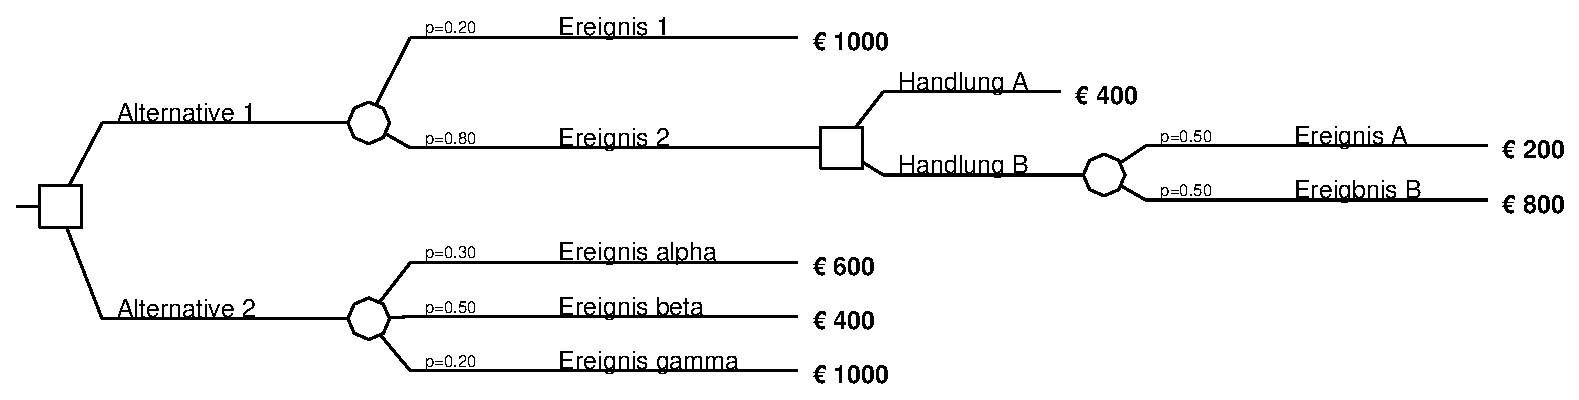
\includegraphics[width=12.5cm]{Grafiken/Klausur.ps}
%\end{center} 
\begin{enumerate}
  \item Sollte die Person an dem weiter rechts liegenden der beiden
  Entscheidungsknoten besser "`Handlung A"' oder "`Handlung B"' wählen?
  \item Wie groß ist der Erwartungswert von "`Alternative 1"' (am ersten
  Entscheidungsknoten von links)?
  \item Sollte die Person "`Alternative 1"' oder "`Alternative 2"' wählen?
\end{enumerate}
(Nehmen Sie dabei an, dass die Person sich rational verhält und den Wert von
zufälligen Ereignissen immer nach dem Erwartungsnutzenprinzip berechnet.)

\subsubsection*{Aufgabe: Nash-Gleichgewichte}

Gegeben sei folgendes Zwei-Personen Spiel:

\begin{center}
\begin{tabular}{c|c|c|}
\multicolumn{1}{c}{} & \multicolumn{1}{c}{$S_1$} &
                               \multicolumn{1}{c}{$S_2$} \\ \cline{2-3} 
$Z_1$                & 1, 1           & 2, 0  \\ \cline{2-3} 
$Z_2$                & 0, 2           & 4, 4  \\ \cline{2-3}
\end{tabular}
\end{center}

\begin{enumerate}
  \item Geben Sie alle {\em reinen} Nash-Gleichgewichte des Spiels an.
  \item Berechnen Sie das {\em gemischte} Nash-Gleichgewicht. Geben Sie an, mit
  welcher Wahrscheinlichkeit der Zeilenspieler im gemischten Gleichgewicht $Z_1$ spielt, und mit welcher 
  Wahrscheinlichkeit der Spaltenspieler im gemischten Gleichgewicht $S_1$ spielt.
\end{enumerate}


\subsubsection*{Aufgabe: Bayes'scher Lehrsatz}

Ein Bergbau-Unternehmen möchte in Sibieren Gold abbauen. Experten schätzen,
dass in dem dafür vorgesehenen Gebiet mit einer Wahrscheinlichkeit von {\bf
30\%} reiche Goldvorkommen zu finden sind. Bevor das Unternehmen jedoch eine
Abbau-Konzession von der Regierung erwirbt, hat es sich das Recht vorbehalten,
Probegrabungen durchzuführen. Falls tatsächlich Goldvorkommen vorhanden
sind, dann liefern die Probegrabungen mit {\bf 95\%} Wahrscheinlichkeit 
ein positives Ergebnis. Allerdings liefern sie mit {\bf 10\%}
Wahrscheinlichkeit auch dann ein positives Ergebnis, wenn in Wirklichkeit kein
Gold vorhanden ist.

\vspace{0.2em}

\setlength{\parindent}{0em}
{\bf Aufgabe:} Mit welcher Wahrscheinlichkeit kann noch davon ausgegangen
werden, dass Gold vorhanden ist, wenn die Probegrabungen ein {\em negatives}
Ergebnis liefern? Stellen Sie zur Lösung der Aufgabe die
entsprechende Rechnung mit Hilfe des Bayes'schen Lehrsatzes auf, und 
rechnen Sie dann die Lösung aus.

\subsubsection*{Aufgabe: Beweise}

\begin{enumerate}
  \item Es seien $x$ und $y$ zwei Güter oder Lotterien mit $x \not\sim y$. Für
  welche Wahrscheinlichkeit $b$ gilt dann: $L(a, x, y) \equiv L(b, y, x)$? Mit
  anderen Worten: Für welchen Wert von $b$ sind die beiden Lotterien über dieselben
  Güter, aber in umgekehrter Reihenfolge identisch?

  \item Die {\em Bedingung der höheren Gewinne} besagt, dass für beliebige
  Lotterien $x$,$y$ und $z$ und jede beliebige Wahrscheinlichkeit $a$ 
  gilt: $x \succ y$ genau dann wenn $L(a, x, z) \succ L(a, y, z)$. 
  (Anders gesagt: Eine Lotterie wir dann vorgezogen, wenn man mit der gleichen 
  Wahrscheinlichkeit auf der {\em ersten} Stelle einen höheren Gewinn erzielen 
  kann, sofern der Gewinn auf der zweiten Stelle derselbe ist.)
  
  {\bf Aufgabe}: Beweisen Sie, dass die Bedingung der höheren Gewinne auch auf der zweiten 
  Stelle gilt, d.h. dass für beliebige Lotterien $x$,$y$
  und $z$ und jede beliebige Wahrscheinlichkeit $a$ gilt: $x \succ y$ genau
  dann wenn $L(a, z, x) \succ L(a, z, y)$.
  
  (Die Gültigkeit der Bedingung der höheren Gewinne auf der ersten Stelle 
   und Ihr Ergebnis der ersten Aufgabe dürfen Sie dabei voraussetzen, aber {\em nicht} den Erwartungsnutzen!)     
\end{enumerate}


\begin{sidewaysfigure}
\begin{center}
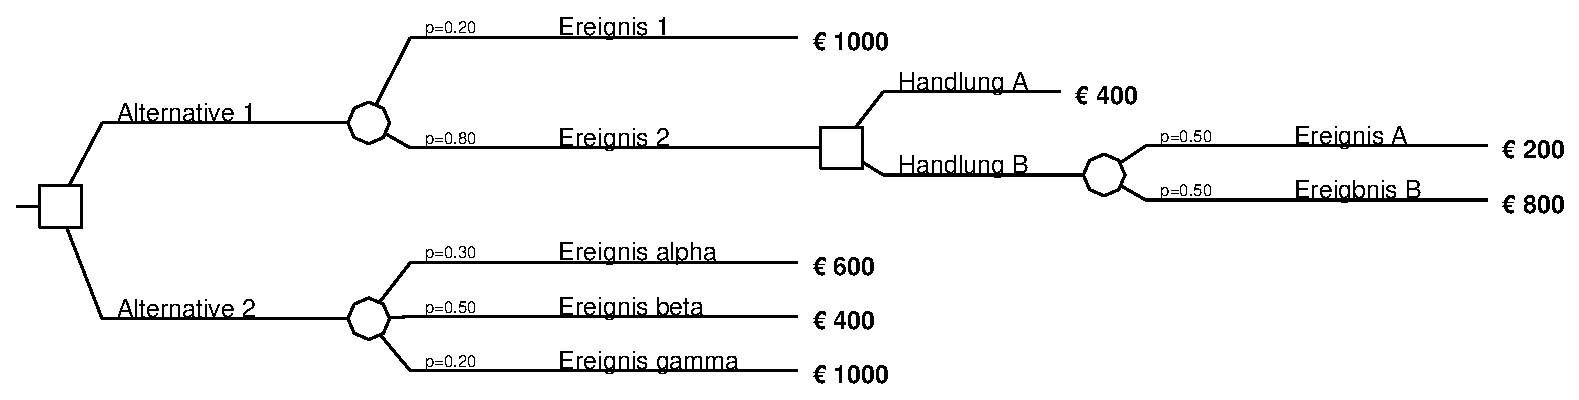
\includegraphics[width=22cm]{Grafiken/Klausur.eps}
\caption{Der Entscheidungsbaum zu Aufgabe \ref{BaumAufgabe}.}
\end{center}
\end{sidewaysfigure}

\newpage
\subsection{Die Lösung}

\subsubsection*{Aufgabe: Entscheidungen unter Unwissenheit}

Bedauernstabelle:

\begin{center}
\begin{tabular}{c|c|c|c|c|}
\multicolumn{1}{c}{} & \multicolumn{1}{c}{$S_1$}
& \multicolumn{1}{c}{$S_2$} & \multicolumn{1}{c}{$S_3$}
& \multicolumn{1}{c}{$S_4$}
\\ \cline{2-5}
$A_1$ & {\bf {\em 197}} &   93 &          0 & 46 \\ \cline{2-5} 
$A_2$ &   0             &    0 &  {\em 497} &  0 \\ \cline{2-5}
$A_3$ &  50             &   40 &  {\em 498} & 25 \\ \cline{2-5}
\end{tabular}
\end{center}

Lösung: {\bf $A_1$} sollte gewählt werden, da bei $A_1$ der maximale
Gewinn, der entegehen könnte, mit 197 kleiner ist als bei $A_2$ mit
497 und $A_3$ mit 498.


\subsubsection*{Entscheidungsbäume}

\begin{enumerate}
\item Für den Erwartungswert der "`Handlung B"' gilt: $EW = 0.5 \cdot
  200 + 0.5 \cdot 800 = 500$ €.  Da die "`Handlung A"' nur 400 €
  liefert, würde eine rational handelnde Person die "`Handlung B"'
  wählen.

\item Es kann davon ausgegangen werden, dass die Personen von den
  beiden Handlungen des rechten Entscheidungsknotens die bessere
  wählt. Damit hat "`Ereignis 1"', wenn es eintritt, einen Wert von
  500 € (siehe die erste Aufgabe). Der Erwartungswert der
  "`Alternative 1"' des linken Entscheidungsknotens berechnet sich
  dann wie gehabt: $EW = 0.2 \cdot 1000 + 0.8 \cdot 500 = 600$ €

\item Um diese Frage zu beantworten, muss nur noch der Erwartungswert
  von "`Alternative 2"' berechnet werden: $EW = 0.3 \cdot 600 + 0.5
  \cdot 400 + 0.2 \cdot 1000 = 580$ €. Da die "`Alternative 1"' einen
  höheren Erwartungswert hat, sollte "`Alternative 1"' gewählt werden.
\end{enumerate}


\subsubsection*{Nash-Gleichgewichte}

\begin{enumerate}
\item Die beiden reinen Nash-Gleichgewichte sind ($Z_1,S_1$) und
  ($Z_2,S_2$). Weder der Zeilen- noch der Spaltenspieler kann sich im
  Gleichgewicht durch einen Wechsel seiner Strategie noch verbessern,
  wenn der andere Spieler seine Strategie beibehält.

\item Ansatz: Ein gemischtes Gleichgewicht kann nur dann vorkommen,
  wenn der jeweils andere Spieler bezüglich der gemischten
  Gleichgewichtsstrategie seines Gegenüber indifferent zwischen seinen
  reinen Strategien ist. Sei $a$ die Wahrscheinlichkeit, mit der der
  Zeilenspieler die erste seiner beiden Strategien $Z_1$ spielt. Dann
  errechnet sich die Auszahlung, die der Spaltenspieler erhält, wenn
  er die Strategie $S_1$ spielt nach:
\[ V(S_1) = a \cdot 1 + (1-a)\cdot 2 \]
  Und die Auszahlung, die er erhält, wenn er $S_2$ spielt, ist:
\[ V(S_2) = a \cdot 0 + (1-a)\cdot 4 \]
  Durch Gleichsetzen erhält man:
\begin{eqnarray}
a \cdot 1 + (1-a)\cdot 2 & = & (1-a)\cdot 4 \\
                  -a + 2 & = & 4 - 4a \\
                      3a & = & 2 \\
                       a & = & \frac{2}{3}
\end{eqnarray}
Im gemischten Gleichgewicht wird der Zeilenspieler also mit 2/3
Wahrscheinlichkeit $Z_1$ spielen und mit 1/3 Wahrscheinlichkeit
$Z_2$. Wegen der Symmetrie des Spiels spielt der Spaltenspieler mit
genau denselben Wahrscheinlichkeiten, nämlich mit 2/3
Wahrscheinlichkeit $S_1$ und mit 1/3 Wahrscheinlichkeit $S_2$.

\end{enumerate}

\subsubsection*{Aufgabe: Bayes'scher Lehrsatz}

Sei $p$ das Ereignis, dass die Probegrabung erfolgreich ausfällt und
$g$ das Ereignis, dass Gold vorhanden ist. Berechnet werden soll die
Wahrscheinlichkeit, dass Gold vorhanden ist, wenn die Probegrabung
negativ ausfällt, d.h. $P(g|\neg p)$. Nach dem Bayes'schen Lehrsatz
gilt:
\[ P(g|\neg p) = \frac{P(\neg p|g)P(g)}{P(\neg p|g)P(g) + P(\neg
  p|\neg g)P(\neg g)} \] 
Aus der Aufgabenstellung geht unmittelbar nur
hervor, dass $P(g)=0.3$, $P(p|g)=0.95$ und $P(p|\neg g)=0.1$. Alle
anderen benötigten Werte muss man aus diesen gegebenen Werten
berechnen, also:
\[ P(\neg g) = 1 - P(g) = 1 - 0,3 = 0,7 \]
\[ P(\neg p|g) = 1 - P (p|g) = 1- 0,95 = 0,05 \]
\[ P(\neg p|\neg g) = 1 - P(p|\neg g) = 1 - 0,1 = 0,9 \]
Durch Einsetzen erhalten wir:
\[ P(g|\neg p) = \frac{0,05 \cdot 0,3}{0,05 \cdot 0,3 + 0,9 \cdot 0,7}
= 0,023256 \] 
Die Lösung lautet also, dass nur noch mit ca. 2,3\%
Wahrscheinlichkeit davon ausgegangen werden kann, dass Gold vorhanden
ist, wenn die Probegrabung negativ ausfällt.

\subsubsection*{Aufgabe: Beweise}

\begin{enumerate}

\item $L(a,x,y) \equiv L(b,y,x)$ wenn $b = 1-a$. Begründung: Wenn
  $b=1-a$, dann kann man in beiden Lotterien mit genau denselben
  Gewinnchancen dieselben Gewinne bekommen. Damit sind die Lotterien
  aber identisch. 

  \begin{small}
  {\em Anmerkung}: Man kann in diesem Fall schon deshalb nicht mit dem
  Erwartungsnutzen argumentieren, weil damit höchstens die Indifferenz 
  zwischen beiden Lotterien gezeigt werden kann, aber noch nicht ihre Identität.
  (Wenn der Erwartungsnutzen von einem Apfel für eine bestimmte Person
  derselbe ist wie der von einer Birne, dann ist die Person zwischen Apfel und
  Birne indifferent, aber deshalb ist ein Apfel noch lange keine Birne!)
  \end{small}

\item Nach dem ersten Teil der Aufgabe ist die Lotterie $L(a, z, x)$ identisch
mit der Lotterie $L(1-a, x, z)$ und die Lottiere $L(a, z, y)$ identisch mit der
      Lotterie $L(1-a, y, z)$.

      Nun gilt aber: Für jedes $a$ mit $0 \leq a \leq 1$ liegt der Wert
      $1-a$ wieder in dem Intervall von 0 bis 1. Dann gilt aber nach der Bedingung der
      höheren Gewinne auf der ersten Stelle (Voraussetzung):
      \[x \succ y \Leftrightarrow L(1-a, x, z) \succ L(1-a, y, z)\]
      Aufgrund der oben festgestellten Identität gilt aber ebenfalls:
      \[L(1-a, x, z) \succ L(1-a, y, z) \Leftrightarrow
        L(a, z, x) \succ L(a, z, y)\]
      Damit gilt insgesamt:
      \[x \succ y \Leftrightarrow L(a, z, x) \succ L(a, z, y) \]      
      q.e.d.
      
      \begin{small}
      {\em Anmerkung}: Wichtig ist, dass der Beweis so geführt wird, dass klar
      ist, dass die Formel am Ende auch tatsächlich für alle $a$ gilt!
      \end{small}
\end{enumerate}

  
\bibliographystyle{apsr}
\bibliography{Vorlesung_Entscheidungstheorie}

\end{document}
